% !TEX program = xelatex
\documentclass[UTF8,fontset=fandol,a4paper,11pt]{ctexart}
\usepackage[margin=21mm,top=23mm,bottom=22mm,headheight=16pt]{geometry}
\usepackage{amsmath,amssymb,mathtools,bm}
\usepackage{tikz}
\usetikzlibrary{arrows.meta,calc,angles,quotes,patterns}
\usepackage{xcolor,booktabs,array,longtable,enumitem,fancyhdr,needspace}
\usepackage[unicode,hidelinks]{hyperref}
\definecolor{ink}{HTML}{24343C}
\definecolor{accent}{HTML}{166A70}
\definecolor{muted}{HTML}{65747A}
\definecolor{rulegray}{HTML}{D4DDE0}
\definecolor{warm}{HTML}{966037}
\color{ink}
\setlength{\parindent}{2em}
\setlength{\parskip}{4pt}
\linespread{1.12}
\AtBeginDocument{\setlength{\abovedisplayskip}{6pt plus 2pt minus 1pt}
\setlength{\belowdisplayskip}{6pt plus 2pt minus 1pt}
\setlength{\abovedisplayshortskip}{0pt plus 1pt}
\setlength{\belowdisplayshortskip}{4pt plus 1pt}}
\setlist[enumerate]{label=(\arabic*),leftmargin=2.3em,itemsep=3pt,topsep=4pt}
\setlist[itemize]{leftmargin=2em,itemsep=2pt,topsep=4pt}
\allowdisplaybreaks[1]
\setlength{\emergencystretch}{2em}
\setcounter{secnumdepth}{0}
\providecommand{\tightlist}{\setlength{\itemsep}{0pt}\setlength{\parskip}{0pt}}
\ctexset{section={format=\Large\bfseries\color{accent},beforeskip=10pt,afterskip=9pt},
subsection={format=\normalsize\bfseries\color{accent},beforeskip=10pt,afterskip=4pt},
subsubsection={format=\normalsize\bfseries,beforeskip=8pt,afterskip=3pt}}
\pagestyle{fancy}
\fancyhf{}
\fancyhead[L]{\small\color{muted}物理学难题集萃}
% 页眉仅保留书名；版本名称只在封面显示。
\fancyfoot[L]{\small\color{muted}\chapterlabel}
\fancyfoot[R]{\small\thepage}
\renewcommand{\headrulewidth}{0.4pt}
\renewcommand{\footrulewidth}{0pt}
\newcommand{\dd}{\mathop{}\!\mathrm{d}}
\newcommand{\vect}[1]{\bm{#1}}
\newcommand{\tagline}[1]{\noindent{\small\color{muted}#1}\par}
\newcommand{\result}[1]{\begin{equation*}\boxed{#1}\end{equation*}}
\newcommand{\figcaption}[1]{\par\vspace{2pt}{\small\color{muted}#1}\par}
\newcommand{\teach}[2]{\Needspace{4\baselineskip}\subsection*{讲解要点与追问}#1\par\smallskip\noindent\textbf{追问：}#2\par}
\newcommand{\workarea}{\par\vspace{7mm}\noindent{\small\color{muted}作答区}\par\vspace{4mm}
\noindent\textcolor{rulegray}{\rule{\linewidth}{0.3pt}}\par\vspace{16mm}
\noindent\textcolor{rulegray}{\rule{\linewidth}{0.3pt}}\par\vspace{16mm}
\noindent\textcolor{rulegray}{\rule{\linewidth}{0.3pt}}\par\vspace{16mm}
\noindent\textcolor{rulegray}{\rule{\linewidth}{0.3pt}}}
\tikzset{axis/.style={-{Stealth[length=2mm]},thin,color=muted},
motion/.style={-{Stealth[length=2.3mm]},thick,color=accent},
force/.style={-{Stealth[length=2.3mm]},thick,color=warm},
traj/.style={thick,color=accent},guide/.style={dashed,thin,color=muted},
object/.style={thick,color=ink},every node/.style={font=\small}}\widowpenalty=10000\clubpenalty=10000\displaywidowpenalty=10000\newcommand{\chapterlabel}{综合试题（四）}







\hypersetup{pdftitle={综合试题（四）·教师版},pdfauthor={}}

\begin{document}\pdfbookmark[0]{综合试题（四）}{cover}

\thispagestyle{empty}\vspace*{22mm}

\noindent{\Huge\bfseries 物理学难题集萃}\par\vspace{12mm}

\noindent{\LARGE 综合试题（四）}\par\vspace{12mm}

\noindent{\Large\color{accent}教师版}\par\vspace{9mm}

\noindent\textcolor{accent}{\rule{\linewidth}{1pt}}\par\vspace{9mm}

\noindent 第1--6题\par\vfill\clearpage

\pdfbookmark[1]{题目目录}{contents}\section*{题目目录}

\begin{longtable}{@{}r p{113mm} r@{}}\toprule 题号 & 题目 & 页码\\\midrule

\hyperref[q:1]{1} & \hyperref[q:1]{由几何约束与自相似计算转动惯量} & \pageref{q:1} \\

\hyperref[q:2]{2} & \hyperref[q:2]{方截面浮木的平衡与临界稳定性} & \pageref{q:2} \\

\hyperref[q:3]{3} & \hyperref[q:3]{滑动悬点细杆的周期与整体落地} & \pageref{q:3} \\

\hyperref[q:4]{4} & \hyperref[q:4]{环形轨道上的连续喷珠与回收} & \pageref{q:4} \\

\hyperref[q:5]{5} & \hyperref[q:5]{二维静电场的通量、场能与带电圆环} & \pageref{q:5} \\

\hyperref[q:6]{6} & \hyperref[q:6]{相对论库仑轨道的近日点进动} & \pageref{q:6} \\

\bottomrule\end{longtable}

\clearpage

\pdfbookmark[2]{第 1 题 由几何约束与自相似计算转动惯量}{q1}

\section*{第 1 题\quad 由几何约束与自相似计算转动惯量}\label{q:1}


（1）一不规则、未必匀质的薄板内有三点$P_1,P_2,P_3$，满足
$P_1P_2=2l,\ P_2P_3=l,\ P_3P_1=\sqrt3l$。薄板质量为$m$，绕过质心$C$且垂直板面的轴转动惯量为$I_C$，已知绕过$P_1,P_2$的平行轴分别有
\[
I_1=I_C+ml^2,\qquad I_2=I_C+3ml^2.
\]
求绕过$P_3$的平行轴转动惯量$I_3$，并讨论结果是否唯一。

（2）均匀薄球壳质量$m$、半径$R$，求绕任一直径的转动惯量。另有半长轴$A$、半短轴$B$、质量$m$的椭圆细环，其质量未必均匀；已知绕长轴的转动惯量$I_A$，求绕短轴的$I_B$。

（3）均匀立方体质量$m$、边长$a$，求绕体对角线$PQ$的转动惯量。要求用量纲、自相似分割和平行轴定理推导系数。


\begin{center}\begin{minipage}{.98\linewidth}\centering
\begin{tikzpicture}[scale=.8,transform shape]

\coordinate (P1) at (0,2);\coordinate (P2) at (0,0);\coordinate (P3) at (.866,.5);
\draw[object] (P1)--(P2)--(P3)--cycle;
\fill (P1) circle (2pt) node[above] {$P_1$};
\fill (P2) circle (2pt) node[below] {$P_2$};
\fill (P3) circle (2pt) node[right] {$P_3$};
\node[left] at (0,1) {$2l$};\node[above right] at (.55,1.4) {$\sqrt3l$};
\node[below right] at (.45,.2) {$l$};

\begin{scope}[xshift=3.4cm]
\draw[object] (0,1) circle (.85);
\draw[guide] (-1,1)--(1,1);
\node at (0,-.3) {薄球壳};
\draw[object] (0,-2) ellipse (1.2 and .6);
\draw[guide] (-1.4,-2)--(1.4,-2) node[right] {$A$};
\draw[guide] (0,-2.8)--(0,-1.2) node[above] {$B$};
\end{scope}
\begin{scope}[xshift=6.4cm]
\begin{scope}[x={(2.2cm,0cm)},y={(1cm,.8cm)},z={(0cm,2.2cm)}]
\draw[object] (0,0,0)--(1,0,0)--(1,0,1)--(0,0,1)--cycle;
\draw[object] (0,0,1)--(0,1,1)--(1,1,1)--(1,0,1);
\draw[object] (1,0,0)--(1,1,0)--(1,1,1);
\draw[guide] (0,0,0)--(0,1,0)--(0,1,1) (0,1,0)--(1,1,0);
\draw[motion] (0,0,0)--(1,1,1);
\node[below left] at (0,0,0) {$P$};\node[above right] at (1,1,1) {$Q$};
\end{scope}\end{scope}

\end{tikzpicture}
\figcaption{图综四.1\quad 三点轴距、薄球壳与椭圆环及体对角线PQ，分属三问。}
\end{minipage}\end{center}

\Needspace{8\baselineskip}

\pdfbookmark[3]{题型定位}{q1-h0}

\subsection*{题型定位}

从质元到整体的三种惯量计算：已知平行轴惯量把质心定位成两圆交点，逐质元几何恒等式形成球壳与椭圆环的惯量关系，自相似立方体分块确定无量纲系数。各问分别使用距离约束、几何求和和尺度可加性。

\Needspace{8\baselineskip}

\pdfbookmark[3]{知识点}{q1-h1}

\subsection*{知识点}

平行轴定理中的$d$是两平行轴间垂距，薄板垂直轴对应质心到指定点的面内距离。惯量对质量可加，逐质元的坐标平方恒等式可乘$\mathrm dm$后积分。球壳三径求和使用$r=R$，三径相等再使用均匀分布的旋转对称性。椭圆的缩放坐标平方和处处为1，任意质量分布都给相同的线性组合。量纲先给$I=\alpha ma^2$，每个自相似小块同时缩放质量与长度平方，系数由平行轴求和确定。

\Needspace{8\baselineskip}

\pdfbookmark[3]{物理图像}{q1-h2}

\subsection*{物理图像}

解图综四.1A中两个候选质心到$P_1,P_2$的距离分别相同，但到右侧$P_3$的距离不同。解图B分别画球壳三条直径和椭圆上的单个质元，将两个几何恒等式对应到惯量积分。解图C把八个小立方体分为两块共轴、六块偏轴；D将偏轴块中心$G$向$PQ$作垂足$H$，平移距离为$GH$。

\Needspace{8\baselineskip}

\pdfbookmark[3]{解题入口}{q1-h3}

\subsection*{解题入口}

从$I_i-I_C$除以$m$读出距离平方，再联立两个圆方程求质心的两个横坐标符号。球壳先把三轴对每个质元的贡献相加，最后用均匀性令三者相等。椭圆先写$x^2/A^2+y^2/B^2=1$再作质量积分。立方体将整块与小块写成同一$\alpha$，分别列小块自身惯量和偏轴平移项，组成闭合方程。

\Needspace{8\baselineskip}

\pdfbookmark[3]{标准解法}{q1-h4}

\subsection*{标准解法}


图综四.1把薄板内的三点、薄球壳与椭圆环及立方体分开表示；薄板转轴垂直板面，球壳取直径，椭圆环则取面内长短轴。
\begin{center}\begin{minipage}{.98\linewidth}\centering
\begin{tikzpicture}[scale=.85,transform shape]

\coordinate (P1) at (0,2);\coordinate (P2) at (0,0);\coordinate (P3) at (.866,.5);
\draw[object] (P1)--(P2)--(P3)--cycle;
\fill (P1) circle (2pt) node[above] {$P_1$};
\fill (P2) circle (2pt) node[below] {$P_2$};
\fill (P3) circle (2pt) node[right] {$P_3$};

\draw[guide] (0,2) circle (1);\draw[guide] (0,0) circle (1.732);
\fill[accent] (.866,1.5) circle (2pt) node[right] {$C_+$};
\fill[warm] (-.866,1.5) circle (2pt) node[left] {$C_-$};
\draw[traj] (.866,.5)--(.866,1.5);
\draw[force] (.866,.5)--(-.866,1.5);
\node[align=left] at (4,1) {$P_3C_+=l$\\$P_3C_-=2l$\\质心有两个候选位置};

\end{tikzpicture}
\figcaption{解图综四.1A\quad 两个惯量条件对应两圆相交，每个交点分别给出一个候选质心。}
\end{minipage}\end{center}
第（1）问，平行轴定理给$I_i=I_C+m(P_iC)^2$。已知两式等价于
\[
P_1C=l,\qquad P_2C=\sqrt3l.
\]
质心$C$同时满足两个距离条件，位于两圆的交点之一。解图综四.1A取
$P_2=(0,0),P_1=(0,2l)$，令$P_3$位于右侧。由两点距离解得
\[
P_3=\left(\frac{\sqrt3}2l,\frac12l\right).
\]
质心$(x_C,y_C)$满足
\[
x_C^2+(y_C-2l)^2=l^2,\qquad x_C^2+y_C^2=3l^2.
\]
将第一式展开为$x_C^2+y_C^2-4ly_C+4l^2=l^2$，再减去第二式，得到$-4ly_C+4l^2=-2l^2$，所以$y_C=3l/2$。回代$x_C^2+y_C^2=3l^2$，有$x_C^2=3l^2/4$，得$x_C=\pm\sqrt3l/2$。两圆关于直线$P_1P_2$对称，其交点的横坐标符号相反；$P_3$取右侧后，两个质心到它的距离自然不同。记为$C_+,C_-$，于是
\[
P_3C_+=l,\qquad P_3C_-=2l.
\]
同侧的$C_+$与$P_3$横坐标相同，两者纵坐标差为$l$；另一侧$C_-$与$P_3$的横坐标差为$\sqrt3l$、纵坐标差为$l$，故距离为$2l$。这也对应三个边长分别为$l,\sqrt3l,2l$的全等直角三角形。再次应用平行轴定理，
\[
\boxed{I_3=I_C+ml^2\quad\text{或}\quad I_C+4ml^2}.
\]
两种质心都满足已知惯量。补充质心所在半平面或质量分布条件后可进一步选择；现有两个距离约束给出两个候选值。
\begin{center}\begin{minipage}{.98\linewidth}\centering
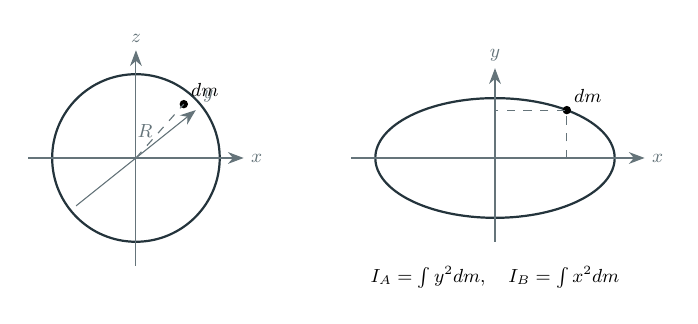
\begin{tikzpicture}[scale=.76,transform shape]

\draw[object] (0,0) circle (1.4);
\draw[axis] (-1.8,0)--(1.8,0) node[right] {$x$};
\draw[axis] (0,-1.8)--(0,1.8) node[above] {$z$};
\draw[axis] (-1,-.8)--(1, .8) node[above right] {$y$};
\fill (.8,.9) circle (2pt) node[above right] {$dm$};
\draw[guide] (0,0)--(.8,.9) node[midway,left] {$R$};
\begin{scope}[xshift=6cm]
\draw[object] (0,0) ellipse (2 and 1);
\draw[axis] (-2.4,0)--(2.5,0) node[right] {$x$};
\draw[axis] (0,-1.4)--(0,1.5) node[above] {$y$};
\fill (1.2,.8) circle (2pt) node[above right] {$dm$};
\draw[guide] (1.2,0)--(1.2,.8)--(0,.8);
\node at (0,-2) {$I_A=\int y^2dm,\quad I_B=\int x^2dm$};
\end{scope}

\end{tikzpicture}
\figcaption{解图综四.1B\quad 球壳三径求和与椭圆上的逐质元几何恒等式。}
\end{minipage}\end{center}
第（2）问，解图综四.1B以球心为原点作三条正交直径。任一质元$dm$的坐标满足$x^2+y^2+z^2=R^2$，所以
\[
I_x=\int(y^2+z^2)dm,\quad
I_y=\int(z^2+x^2)dm,\quad
I_z=\int(x^2+y^2)dm.
\]
相加得
\[
I_x+I_y+I_z=2\int R^2dm=2mR^2.
\]
均匀球壳关于任一直径的惯量相同，$I_x=I_y=I_z=I_R$，故
\[
\boxed{I_R=\frac23mR^2}.
\]
求和时每个坐标平方恰出现两次，所以几何恒等式适用于壳上的每一个质元。其后使用均匀分布的旋转对称性，将三条直径的惯量置为相同，再由总和除以3。这里先作逐质元求和、后使用质量对称性，这两步分别给出$2mR^2$和三径相等。

对解图综四.1B右侧的椭圆细环，取长轴为$x$轴、短轴为$y$轴。每个质元都满足
$x^2/A^2+y^2/B^2=1$，而
\[
I_A=\int y^2dm,\qquad I_B=\int x^2dm.
\]
将几何恒等式按质量积分：
\[
\frac{I_A}{B^2}+\frac{I_B}{A^2}
=\int\left(\frac{y^2}{B^2}+\frac{x^2}{A^2}\right)dm=m.
\]
因此即使质量不均匀，仍有
\[
\boxed{I_B=mA^2-\frac{A^2}{B^2}I_A}.
\]
若弧长线密度为$\lambda(s)$，两项相加后被积函数为$\lambda(s)[x^2/A^2+y^2/B^2]=\lambda(s)$，因此右端恰是总质量。质量偏向长轴端点会增加$I_B$、减小$I_A$，二者始终满足这一线性关系；它保留了题设未指定密度时可确定的全部组合信息。
\begin{center}\begin{minipage}{.98\linewidth}\centering
\begin{tikzpicture}[scale=.85,transform shape]

\begin{scope}[x={(2.2cm,0cm)},y={(1cm,.8cm)},z={(0cm,2.2cm)}]
\draw[object] (0,0,0)--(1,0,0)--(1,0,1)--(0,0,1)--cycle;
\draw[object] (0,0,1)--(0,1,1)--(1,1,1)--(1,0,1);
\draw[object] (1,0,0)--(1,1,0)--(1,1,1);
\draw[guide] (0,0,0)--(0,1,0)--(0,1,1) (0,1,0)--(1,1,0);
\draw[motion] (0,0,0)--(1,1,1);
\node[below left] at (0,0,0) {$P$};\node[above right] at (1,1,1) {$Q$};

\draw[guide] (.5,0,0)--(.5,0,1)--(.5,1,1)--(.5,1,0)--cycle;
\draw[guide] (0,.5,0)--(1,.5,0)--(1,.5,1)--(0,.5,1)--cycle;
\draw[guide] (0,0,.5)--(1,0,.5)--(1,1,.5)--(0,1,.5)--cycle;
\fill[accent] (.25,.25,.25) circle (1.5pt) (.75,.75,.75) circle (1.5pt);
\end{scope}
\node[align=left] at (6,1.7) {两块中心在PQ上\\六块中心偏离PQ\\$I'=\alpha ma^2/32$\\$d=a/\sqrt6$};
\node at (3,-1) {$I=8I'+6(m/8)d^2$};

\end{tikzpicture}
\figcaption{解图综四.1C\quad 八个小立方体共享同一个无量纲惯量系数，偏轴六块再加平移项。}
\end{minipage}\end{center}
第（3）问，立方体只有质量尺度$m$与长度尺度$a$，故绕给定体对角线的惯量应写为
$I=\alpha ma^2$。量纲给不出无量纲常数$\alpha$，还要使用自相似分割。

解图综四.1C将立方体沿三方向各平分成八块。每块质量$m/8$、边长$a/2$，绕自身、平行于$PQ$的体对角线有
\[
I'=\alpha\frac m8\left(\frac a2\right)^2=\frac{\alpha ma^2}{32}.
\]
八个小立方体中两块的中心落在$PQ$上；另外六块中心到$PQ$的垂距相同；每块自己的体对角线方向与大轴平行，正好满足平行轴定理的轴向条件。以大立方体中心为原点，后六个中心坐标是$(\pm a/4,\pm a/4,\pm a/4)$中符号不全相同者。沿$PQ$的单位向量为$(1,1,1)/\sqrt3$，所以
\[
d^2=\frac{3a^2}{16}
-\frac{(a/4)^2}{3}=\frac{a^2}{6}.
\]
解图综四.1D把偏轴小块中心$G$到大轴的垂足$H$标出，$GH$才是平移项所用的距离。由直角分解$GH^2=OG^2-OH^2$得到上式，也可写成$d=(a/2)\sqrt{2/3}=a/\sqrt6$。
\begin{center}\begin{minipage}{.98\linewidth}\centering
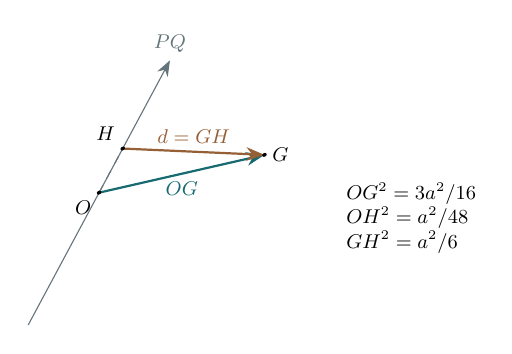
\begin{tikzpicture}[scale=0.8,transform shape]
\begin{scope}[x={(1cm,0cm)},y={(.25cm,.9cm)},z={(-.5cm,.5cm)}]
\coordinate (O) at (0,0,0);\coordinate (G) at (1.5,1.5,-1.5);\coordinate (H) at (.5,.5,.5);
\draw[axis] (-1.5,-1.5,-1.5)--(1.5,1.5,1.5) node[above] {$PQ$};
\draw[motion] (O)--(G) node[midway,below] {$OG$};\draw[guide] (O)--(H);
\draw[force] (H)--(G) node[midway,above] {$d=GH$};
\fill (O) circle(.035) node[below left] {$O$};\fill (G) circle(.035) node[right] {$G$};\fill (H) circle(.035) node[above left] {$H$};\end{scope}
\node[right,align=left] at (3.8,-.4) {$OG^2=3a^2/16$\\$OH^2=a^2/48$\\$GH^2=a^2/6$};\end{tikzpicture}
\figcaption{解图综四.1D\quad 偏轴小块中心向大体对角线投影，平移项取垂距GH的平方}
\end{minipage}\end{center}
每个偏轴小块由平行轴定理增加$(m/8)d^2=ma^2/48$，相加得
\[
I=2I'+6\left(I'+\frac{ma^2}{48}\right)
=8I'+\frac{ma^2}{8}.
\]
代入$I=\alpha ma^2$和$I'=\alpha ma^2/32$，
\[
\alpha=\frac{\alpha}{4}+\frac18,\qquad
\boxed{\alpha=\frac16,\quad I=\frac16ma^2}.
\]
均匀立方体的中心惯量还可由其对称性解释：三坐标方向的二次矩各为$\int x^2\,\mathrm dm=ma^2/12$，故$I_x=I_y=I_z=ma^2/6$。关于中心平面的反射使$\int xy\,\mathrm dm$等混合二次矩为零。对于任意单位轴向$\boldsymbol n$，$I_{\boldsymbol n}=n_x^2I_x+n_y^2I_y+n_z^2I_z=ma^2/6$；因此体对角线与其他中心轴具有相同的惯量。


\Needspace{8\baselineskip}

\pdfbookmark[3]{关键洞察}{q1-h5}

\subsection*{关键洞察}

两个惯量条件分别给一条质心距离约束，几何对称产生两个候选位置；第三点偏在一侧，使第三惯量有两个值。椭圆环的结论由每处均成立的几何式决定，球壳三径相等则另含均匀条件。小立方体的惯量相对于整块缩小$1/32$，其中质量缩小$1/8$、长度平方缩小$1/4$。

\Needspace{8\baselineskip}

\pdfbookmark[3]{易错点}{q1-h6}

\subsection*{易错点}

薄板轮廓用于表示对象，质心的选择按给定的距离数据；补充半平面或密度信息后再选择分支。球壳的质元都在$r=R$，对应$2mR^2/3$。非均匀椭圆环保留完整积分关系，具体$I_A$由其质量分布决定。八块都计自身惯量，仅六块追加垂距平移项；$OG$为中心距离，$GH$为所需轴距。

\Needspace{8\baselineskip}

\pdfbookmark[3]{课堂讲解建议}{q1-h7}

\subsection*{课堂讲解建议}

先让学生用圆规作出两个候选质心，再问哪一项补充条件能唯一选择，学生可回答质心位于直线$P_1P_2$的哪一侧。球壳部分让学生写一个质元对三径的贡献和，随后指出使用均匀性的具体一步：逐质元几何求和适用于任意质量分布，三条直径惯量相等这一步使用均匀性。椭圆换成非均匀线密度仍作同一加权积分，说明几何恒等式的作用。最后用两色标八个小立方体，分别报质量、边长、轴距，再解$\alpha$。追问量纲为何只给$ma^2$，让学生说明数值系数还由质量分布与平行轴项决定；图D的垂足使平移项有直观对应。

\Needspace{8\baselineskip}

\pdfbookmark[3]{变式训练}{q1-h8}

\subsection*{变式训练}

\begin{enumerate}
\Needspace{37\baselineskip}
\item \textbf{题设与求解。} 另知质心在$P_1P_2$直线的哪一侧，第三惯量如何确定？与$P_3$同侧时取$C_+$，距离$P_3C_+=l$，故$I_3=I_C+ml^2$；异侧取$C_-$，距离为$2l$，故$I_3=I_C+4ml^2$。两候选值之差为$3ml^2$，与$I_C$无关。图综四.1V1以同一$P_3$连接两候选质心，半平面信息恰好选择一个距离。
\begin{center}\begin{minipage}{.98\linewidth}\centering
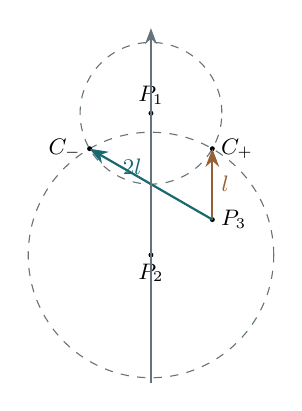
\begin{tikzpicture}[scale=0.9,transform shape]
\draw[guide] (0,2) circle(1);\draw[guide] (0,0) circle(1.7320508075688772);
\fill (0,2) circle(.035) node[above] {$P_1$};\fill (0,0) circle(.035) node[below] {$P_2$};
\fill (0.8660254037844386,.5) circle(.035) node[right] {$P_3$};\fill (0.8660254037844386,1.5) circle(.035) node[right] {$C_+$};
\fill (-0.8660254037844386,1.5) circle(.035) node[left] {$C_-$};
\draw[force] (0.8660254037844386,.5)--(0.8660254037844386,1.5) node[midway,right] {$l$};
\draw[motion] (0.8660254037844386,.5)--(-0.8660254037844386,1.5) node[midway,above left] {$2l$};
\draw[axis] (0,-1.8)--(0,3.2);\end{tikzpicture}
\figcaption{解图综四.1V1\quad 质心所在半平面选择到P3的两种距离}
\end{minipage}\end{center}
\Needspace{37\baselineskip}
\item \textbf{题设与求解。} 椭圆退化为半径$R$的圆环，线密度按$\lambda(\varphi)=\lambda_0[1+\epsilon\cos2\varphi]$分布，$|\epsilon|\leqslant1$。由总质量$m=2\pi R\lambda_0$，\[
I_x=\frac{mR^2}{2\pi}\int_0^{2\pi}\sin^2\varphi(1+\epsilon\cos2\varphi)\,\mathrm d\varphi
=mR^2\left(\frac12-\frac\epsilon4\right),
\]
同理$I_y=mR^2(1/2+\epsilon/4)$，故始终$I_x+I_y=mR^2$。关于两坐标轴反射对称使混合惯性积为零；再具备90度旋转对称时给出$I_x=I_y=mR^2/2$。图V2画两个惯量随$\epsilon$的互补变化，区分求和关系与两轴相等所需条件。
\begin{center}\begin{minipage}{.98\linewidth}\centering
\begin{tikzpicture}[scale=0.72,transform shape]
\draw[axis] (0,0)--(6.2,0);\draw[axis] (0,0)--(0,3.4000000000000004);
\draw[thin,color=muted] (0.0000000,0)--(0.0000000,-.07);\node[below] at (0.0000000,-.09) {$-1$};
\draw[thin,color=muted] (3.0000000,0)--(3.0000000,-.07);\node[below] at (3.0000000,-.09) {$0$};
\draw[thin,color=muted] (6.0000000,0)--(6.0000000,-.07);\node[below] at (6.0000000,-.09) {$1$};
\draw[thin,color=muted] (0,0.2666667)--(-.07,0.2666667);\node[left] at (-.09,0.2666667) {$1/4$};
\draw[thin,color=muted] (0,1.6000000)--(-.07,1.6000000);\node[left] at (-.09,1.6000000) {$1/2$};
\draw[thin,color=muted] (0,2.9333333)--(-.07,2.9333333);\node[left] at (-.09,2.9333333) {$3/4$};
\node[below] at (3.0,-.64) {密度参数$\epsilon$};\node[above right] at (0,3.45) {$I/(mR^2)$};
\draw[traj] plot coordinates {(0.0000000,2.9333333) (0.0300000,2.9200000) (0.0600000,2.9066667) (0.0900000,2.8933333) (0.1200000,2.8800000) (0.1500000,2.8666667) (0.1800000,2.8533333) (0.2100000,2.8400000) (0.2400000,2.8266667) (0.2700000,2.8133333) (0.3000000,2.8000000) (0.3300000,2.7866667) (0.3600000,2.7733333) (0.3900000,2.7600000) (0.4200000,2.7466667) (0.4500000,2.7333333) (0.4800000,2.7200000) (0.5100000,2.7066667) (0.5400000,2.6933333) (0.5700000,2.6800000) (0.6000000,2.6666667) (0.6300000,2.6533333) (0.6600000,2.6400000) (0.6900000,2.6266667) (0.7200000,2.6133333) (0.7500000,2.6000000) (0.7800000,2.5866667) (0.8100000,2.5733333) (0.8400000,2.5600000) (0.8700000,2.5466667) (0.9000000,2.5333333) (0.9300000,2.5200000) (0.9600000,2.5066667) (0.9900000,2.4933333) (1.0200000,2.4800000) (1.0500000,2.4666667) (1.0800000,2.4533333) (1.1100000,2.4400000) (1.1400000,2.4266667) (1.1700000,2.4133333) (1.2000000,2.4000000) (1.2300000,2.3866667) (1.2600000,2.3733333) (1.2900000,2.3600000) (1.3200000,2.3466667) (1.3500000,2.3333333) (1.3800000,2.3200000) (1.4100000,2.3066667) (1.4400000,2.2933333) (1.4700000,2.2800000) (1.5000000,2.2666667) (1.5300000,2.2533333) (1.5600000,2.2400000) (1.5900000,2.2266667) (1.6200000,2.2133333) (1.6500000,2.2000000) (1.6800000,2.1866667) (1.7100000,2.1733333) (1.7400000,2.1600000) (1.7700000,2.1466667) (1.8000000,2.1333333) (1.8300000,2.1200000) (1.8600000,2.1066667) (1.8900000,2.0933333) (1.9200000,2.0800000) (1.9500000,2.0666667) (1.9800000,2.0533333) (2.0100000,2.0400000) (2.0400000,2.0266667) (2.0700000,2.0133333) (2.1000000,2.0000000) (2.1300000,1.9866667) (2.1600000,1.9733333) (2.1900000,1.9600000) (2.2200000,1.9466667) (2.2500000,1.9333333) (2.2800000,1.9200000) (2.3100000,1.9066667) (2.3400000,1.8933333) (2.3700000,1.8800000) (2.4000000,1.8666667) (2.4300000,1.8533333) (2.4600000,1.8400000) (2.4900000,1.8266667) (2.5200000,1.8133333) (2.5500000,1.8000000) (2.5800000,1.7866667) (2.6100000,1.7733333) (2.6400000,1.7600000) (2.6700000,1.7466667) (2.7000000,1.7333333) (2.7300000,1.7200000) (2.7600000,1.7066667) (2.7900000,1.6933333) (2.8200000,1.6800000) (2.8500000,1.6666667) (2.8800000,1.6533333) (2.9100000,1.6400000) (2.9400000,1.6266667) (2.9700000,1.6133333) (3.0000000,1.6000000) (3.0300000,1.5866667) (3.0600000,1.5733333) (3.0900000,1.5600000) (3.1200000,1.5466667) (3.1500000,1.5333333) (3.1800000,1.5200000) (3.2100000,1.5066667) (3.2400000,1.4933333) (3.2700000,1.4800000) (3.3000000,1.4666667) (3.3300000,1.4533333) (3.3600000,1.4400000) (3.3900000,1.4266667) (3.4200000,1.4133333) (3.4500000,1.4000000) (3.4800000,1.3866667) (3.5100000,1.3733333) (3.5400000,1.3600000) (3.5700000,1.3466667) (3.6000000,1.3333333) (3.6300000,1.3200000) (3.6600000,1.3066667) (3.6900000,1.2933333) (3.7200000,1.2800000) (3.7500000,1.2666667) (3.7800000,1.2533333) (3.8100000,1.2400000) (3.8400000,1.2266667) (3.8700000,1.2133333) (3.9000000,1.2000000) (3.9300000,1.1866667) (3.9600000,1.1733333) (3.9900000,1.1600000) (4.0200000,1.1466667) (4.0500000,1.1333333) (4.0800000,1.1200000) (4.1100000,1.1066667) (4.1400000,1.0933333) (4.1700000,1.0800000) (4.2000000,1.0666667) (4.2300000,1.0533333) (4.2600000,1.0400000) (4.2900000,1.0266667) (4.3200000,1.0133333) (4.3500000,1.0000000) (4.3800000,0.9866667) (4.4100000,0.9733333) (4.4400000,0.9600000) (4.4700000,0.9466667) (4.5000000,0.9333333) (4.5300000,0.9200000) (4.5600000,0.9066667) (4.5900000,0.8933333) (4.6200000,0.8800000) (4.6500000,0.8666667) (4.6800000,0.8533333) (4.7100000,0.8400000) (4.7400000,0.8266667) (4.7700000,0.8133333) (4.8000000,0.8000000) (4.8300000,0.7866667) (4.8600000,0.7733333) (4.8900000,0.7600000) (4.9200000,0.7466667) (4.9500000,0.7333333) (4.9800000,0.7200000) (5.0100000,0.7066667) (5.0400000,0.6933333) (5.0700000,0.6800000) (5.1000000,0.6666667) (5.1300000,0.6533333) (5.1600000,0.6400000) (5.1900000,0.6266667) (5.2200000,0.6133333) (5.2500000,0.6000000) (5.2800000,0.5866667) (5.3100000,0.5733333) (5.3400000,0.5600000) (5.3700000,0.5466667) (5.4000000,0.5333333) (5.4300000,0.5200000) (5.4600000,0.5066667) (5.4900000,0.4933333) (5.5200000,0.4800000) (5.5500000,0.4666667) (5.5800000,0.4533333) (5.6100000,0.4400000) (5.6400000,0.4266667) (5.6700000,0.4133333) (5.7000000,0.4000000) (5.7300000,0.3866667) (5.7600000,0.3733333) (5.7900000,0.3600000) (5.8200000,0.3466667) (5.8500000,0.3333333) (5.8800000,0.3200000) (5.9100000,0.3066667) (5.9400000,0.2933333) (5.9700000,0.2800000) (6.0000000,0.2666667)};
\draw[traj] (.1,-1.05)--(.7,-1.05);\node[right] at (.85,-1.05) {$I_x$};\draw[dashed,thick,color=warm] plot coordinates {(0.0000000,0.2666667) (0.0300000,0.2800000) (0.0600000,0.2933333) (0.0900000,0.3066667) (0.1200000,0.3200000) (0.1500000,0.3333333) (0.1800000,0.3466667) (0.2100000,0.3600000) (0.2400000,0.3733333) (0.2700000,0.3866667) (0.3000000,0.4000000) (0.3300000,0.4133333) (0.3600000,0.4266667) (0.3900000,0.4400000) (0.4200000,0.4533333) (0.4500000,0.4666667) (0.4800000,0.4800000) (0.5100000,0.4933333) (0.5400000,0.5066667) (0.5700000,0.5200000) (0.6000000,0.5333333) (0.6300000,0.5466667) (0.6600000,0.5600000) (0.6900000,0.5733333) (0.7200000,0.5866667) (0.7500000,0.6000000) (0.7800000,0.6133333) (0.8100000,0.6266667) (0.8400000,0.6400000) (0.8700000,0.6533333) (0.9000000,0.6666667) (0.9300000,0.6800000) (0.9600000,0.6933333) (0.9900000,0.7066667) (1.0200000,0.7200000) (1.0500000,0.7333333) (1.0800000,0.7466667) (1.1100000,0.7600000) (1.1400000,0.7733333) (1.1700000,0.7866667) (1.2000000,0.8000000) (1.2300000,0.8133333) (1.2600000,0.8266667) (1.2900000,0.8400000) (1.3200000,0.8533333) (1.3500000,0.8666667) (1.3800000,0.8800000) (1.4100000,0.8933333) (1.4400000,0.9066667) (1.4700000,0.9200000) (1.5000000,0.9333333) (1.5300000,0.9466667) (1.5600000,0.9600000) (1.5900000,0.9733333) (1.6200000,0.9866667) (1.6500000,1.0000000) (1.6800000,1.0133333) (1.7100000,1.0266667) (1.7400000,1.0400000) (1.7700000,1.0533333) (1.8000000,1.0666667) (1.8300000,1.0800000) (1.8600000,1.0933333) (1.8900000,1.1066667) (1.9200000,1.1200000) (1.9500000,1.1333333) (1.9800000,1.1466667) (2.0100000,1.1600000) (2.0400000,1.1733333) (2.0700000,1.1866667) (2.1000000,1.2000000) (2.1300000,1.2133333) (2.1600000,1.2266667) (2.1900000,1.2400000) (2.2200000,1.2533333) (2.2500000,1.2666667) (2.2800000,1.2800000) (2.3100000,1.2933333) (2.3400000,1.3066667) (2.3700000,1.3200000) (2.4000000,1.3333333) (2.4300000,1.3466667) (2.4600000,1.3600000) (2.4900000,1.3733333) (2.5200000,1.3866667) (2.5500000,1.4000000) (2.5800000,1.4133333) (2.6100000,1.4266667) (2.6400000,1.4400000) (2.6700000,1.4533333) (2.7000000,1.4666667) (2.7300000,1.4800000) (2.7600000,1.4933333) (2.7900000,1.5066667) (2.8200000,1.5200000) (2.8500000,1.5333333) (2.8800000,1.5466667) (2.9100000,1.5600000) (2.9400000,1.5733333) (2.9700000,1.5866667) (3.0000000,1.6000000) (3.0300000,1.6133333) (3.0600000,1.6266667) (3.0900000,1.6400000) (3.1200000,1.6533333) (3.1500000,1.6666667) (3.1800000,1.6800000) (3.2100000,1.6933333) (3.2400000,1.7066667) (3.2700000,1.7200000) (3.3000000,1.7333333) (3.3300000,1.7466667) (3.3600000,1.7600000) (3.3900000,1.7733333) (3.4200000,1.7866667) (3.4500000,1.8000000) (3.4800000,1.8133333) (3.5100000,1.8266667) (3.5400000,1.8400000) (3.5700000,1.8533333) (3.6000000,1.8666667) (3.6300000,1.8800000) (3.6600000,1.8933333) (3.6900000,1.9066667) (3.7200000,1.9200000) (3.7500000,1.9333333) (3.7800000,1.9466667) (3.8100000,1.9600000) (3.8400000,1.9733333) (3.8700000,1.9866667) (3.9000000,2.0000000) (3.9300000,2.0133333) (3.9600000,2.0266667) (3.9900000,2.0400000) (4.0200000,2.0533333) (4.0500000,2.0666667) (4.0800000,2.0800000) (4.1100000,2.0933333) (4.1400000,2.1066667) (4.1700000,2.1200000) (4.2000000,2.1333333) (4.2300000,2.1466667) (4.2600000,2.1600000) (4.2900000,2.1733333) (4.3200000,2.1866667) (4.3500000,2.2000000) (4.3800000,2.2133333) (4.4100000,2.2266667) (4.4400000,2.2400000) (4.4700000,2.2533333) (4.5000000,2.2666667) (4.5300000,2.2800000) (4.5600000,2.2933333) (4.5900000,2.3066667) (4.6200000,2.3200000) (4.6500000,2.3333333) (4.6800000,2.3466667) (4.7100000,2.3600000) (4.7400000,2.3733333) (4.7700000,2.3866667) (4.8000000,2.4000000) (4.8300000,2.4133333) (4.8600000,2.4266667) (4.8900000,2.4400000) (4.9200000,2.4533333) (4.9500000,2.4666667) (4.9800000,2.4800000) (5.0100000,2.4933333) (5.0400000,2.5066667) (5.0700000,2.5200000) (5.1000000,2.5333333) (5.1300000,2.5466667) (5.1600000,2.5600000) (5.1900000,2.5733333) (5.2200000,2.5866667) (5.2500000,2.6000000) (5.2800000,2.6133333) (5.3100000,2.6266667) (5.3400000,2.6400000) (5.3700000,2.6533333) (5.4000000,2.6666667) (5.4300000,2.6800000) (5.4600000,2.6933333) (5.4900000,2.7066667) (5.5200000,2.7200000) (5.5500000,2.7333333) (5.5800000,2.7466667) (5.6100000,2.7600000) (5.6400000,2.7733333) (5.6700000,2.7866667) (5.7000000,2.8000000) (5.7300000,2.8133333) (5.7600000,2.8266667) (5.7900000,2.8400000) (5.8200000,2.8533333) (5.8500000,2.8666667) (5.8800000,2.8800000) (5.9100000,2.8933333) (5.9400000,2.9066667) (5.9700000,2.9200000) (6.0000000,2.9333333)};
\draw[dashed,thick,color=warm] (.1,-1.48)--(.7,-1.48);\node[right] at (.85,-1.48) {$I_y$};\end{tikzpicture}
\figcaption{解图综四.1V2\quad 非均匀圆环的两轴惯量互补，和由壳面几何固定}
\end{minipage}\end{center}
\Needspace{37\baselineskip}
\item \textbf{题设与求解。} 薄球壳转轴与某条直径平行，距球心为$d$。由平行轴定理，$I(d)=I_R+md^2=2mR^2/3+md^2$。相切轴$d=R$给出$I=5mR^2/3$。图V3画归一化$I/(mR^2)=2/3+(d/R)^2$，最小值在过球心的轴，平移项随轴距平方增加。
\begin{center}\begin{minipage}{.98\linewidth}\centering
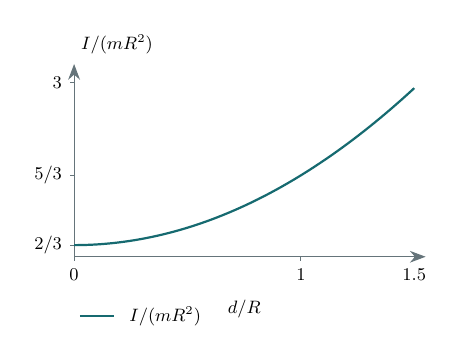
\begin{tikzpicture}[scale=0.72,transform shape]
\draw[axis] (0,0)--(6.2,0);\draw[axis] (0,0)--(0,3.4000000000000004);
\draw[thin,color=muted] (0.0000000,0)--(0.0000000,-.07);\node[below] at (0.0000000,-.09) {$0$};
\draw[thin,color=muted] (4.0000000,0)--(4.0000000,-.07);\node[below] at (4.0000000,-.09) {$1$};
\draw[thin,color=muted] (6.0000000,0)--(6.0000000,-.07);\node[below] at (6.0000000,-.09) {$1.5$};
\draw[thin,color=muted] (0,0.2051282)--(-.07,0.2051282);\node[left] at (-.09,0.2051282) {$2/3$};
\draw[thin,color=muted] (0,1.4358974)--(-.07,1.4358974);\node[left] at (-.09,1.4358974) {$5/3$};
\draw[thin,color=muted] (0,3.0769231)--(-.07,3.0769231);\node[left] at (-.09,3.0769231) {$3$};
\node[below] at (3.0,-.64) {$d/R$};\node[above right] at (0,3.45) {$I/(mR^2)$};
\draw[traj] plot coordinates {(0.0000000,0.2051282) (0.0300000,0.2051974) (0.0600000,0.2054051) (0.0900000,0.2057513) (0.1200000,0.2062359) (0.1500000,0.2068590) (0.1800000,0.2076205) (0.2100000,0.2085205) (0.2400000,0.2095590) (0.2700000,0.2107359) (0.3000000,0.2120513) (0.3300000,0.2135051) (0.3600000,0.2150974) (0.3900000,0.2168282) (0.4200000,0.2186974) (0.4500000,0.2207051) (0.4800000,0.2228513) (0.5100000,0.2251359) (0.5400000,0.2275590) (0.5700000,0.2301205) (0.6000000,0.2328205) (0.6300000,0.2356590) (0.6600000,0.2386359) (0.6900000,0.2417513) (0.7200000,0.2450051) (0.7500000,0.2483974) (0.7800000,0.2519282) (0.8100000,0.2555974) (0.8400000,0.2594051) (0.8700000,0.2633513) (0.9000000,0.2674359) (0.9300000,0.2716590) (0.9600000,0.2760205) (0.9900000,0.2805205) (1.0200000,0.2851590) (1.0500000,0.2899359) (1.0800000,0.2948513) (1.1100000,0.2999051) (1.1400000,0.3050974) (1.1700000,0.3104282) (1.2000000,0.3158974) (1.2300000,0.3215051) (1.2600000,0.3272513) (1.2900000,0.3331359) (1.3200000,0.3391590) (1.3500000,0.3453205) (1.3800000,0.3516205) (1.4100000,0.3580590) (1.4400000,0.3646359) (1.4700000,0.3713513) (1.5000000,0.3782051) (1.5300000,0.3851974) (1.5600000,0.3923282) (1.5900000,0.3995974) (1.6200000,0.4070051) (1.6500000,0.4145513) (1.6800000,0.4222359) (1.7100000,0.4300590) (1.7400000,0.4380205) (1.7700000,0.4461205) (1.8000000,0.4543590) (1.8300000,0.4627359) (1.8600000,0.4712513) (1.8900000,0.4799051) (1.9200000,0.4886974) (1.9500000,0.4976282) (1.9800000,0.5066974) (2.0100000,0.5159051) (2.0400000,0.5252513) (2.0700000,0.5347359) (2.1000000,0.5443590) (2.1300000,0.5541205) (2.1600000,0.5640205) (2.1900000,0.5740590) (2.2200000,0.5842359) (2.2500000,0.5945513) (2.2800000,0.6050051) (2.3100000,0.6155974) (2.3400000,0.6263282) (2.3700000,0.6371974) (2.4000000,0.6482051) (2.4300000,0.6593513) (2.4600000,0.6706359) (2.4900000,0.6820590) (2.5200000,0.6936205) (2.5500000,0.7053205) (2.5800000,0.7171590) (2.6100000,0.7291359) (2.6400000,0.7412513) (2.6700000,0.7535051) (2.7000000,0.7658974) (2.7300000,0.7784282) (2.7600000,0.7910974) (2.7900000,0.8039051) (2.8200000,0.8168513) (2.8500000,0.8299359) (2.8800000,0.8431590) (2.9100000,0.8565205) (2.9400000,0.8700205) (2.9700000,0.8836590) (3.0000000,0.8974359) (3.0300000,0.9113513) (3.0600000,0.9254051) (3.0900000,0.9395974) (3.1200000,0.9539282) (3.1500000,0.9683974) (3.1800000,0.9830051) (3.2100000,0.9977513) (3.2400000,1.0126359) (3.2700000,1.0276590) (3.3000000,1.0428205) (3.3300000,1.0581205) (3.3600000,1.0735590) (3.3900000,1.0891359) (3.4200000,1.1048513) (3.4500000,1.1207051) (3.4800000,1.1366974) (3.5100000,1.1528282) (3.5400000,1.1690974) (3.5700000,1.1855051) (3.6000000,1.2020513) (3.6300000,1.2187359) (3.6600000,1.2355590) (3.6900000,1.2525205) (3.7200000,1.2696205) (3.7500000,1.2868590) (3.7800000,1.3042359) (3.8100000,1.3217513) (3.8400000,1.3394051) (3.8700000,1.3571974) (3.9000000,1.3751282) (3.9300000,1.3931974) (3.9600000,1.4114051) (3.9900000,1.4297513) (4.0200000,1.4482359) (4.0500000,1.4668590) (4.0800000,1.4856205) (4.1100000,1.5045205) (4.1400000,1.5235590) (4.1700000,1.5427359) (4.2000000,1.5620513) (4.2300000,1.5815051) (4.2600000,1.6010974) (4.2900000,1.6208282) (4.3200000,1.6406974) (4.3500000,1.6607051) (4.3800000,1.6808513) (4.4100000,1.7011359) (4.4400000,1.7215590) (4.4700000,1.7421205) (4.5000000,1.7628205) (4.5300000,1.7836590) (4.5600000,1.8046359) (4.5900000,1.8257513) (4.6200000,1.8470051) (4.6500000,1.8683974) (4.6800000,1.8899282) (4.7100000,1.9115974) (4.7400000,1.9334051) (4.7700000,1.9553513) (4.8000000,1.9774359) (4.8300000,1.9996590) (4.8600000,2.0220205) (4.8900000,2.0445205) (4.9200000,2.0671590) (4.9500000,2.0899359) (4.9800000,2.1128513) (5.0100000,2.1359051) (5.0400000,2.1590974) (5.0700000,2.1824282) (5.1000000,2.2058974) (5.1300000,2.2295051) (5.1600000,2.2532513) (5.1900000,2.2771359) (5.2200000,2.3011590) (5.2500000,2.3253205) (5.2800000,2.3496205) (5.3100000,2.3740590) (5.3400000,2.3986359) (5.3700000,2.4233513) (5.4000000,2.4482051) (5.4300000,2.4731974) (5.4600000,2.4983282) (5.4900000,2.5235974) (5.5200000,2.5490051) (5.5500000,2.5745513) (5.5800000,2.6002359) (5.6100000,2.6260590) (5.6400000,2.6520205) (5.6700000,2.6781205) (5.7000000,2.7043590) (5.7300000,2.7307359) (5.7600000,2.7572513) (5.7900000,2.7839051) (5.8200000,2.8106974) (5.8500000,2.8376282) (5.8800000,2.8646974) (5.9100000,2.8919051) (5.9400000,2.9192513) (5.9700000,2.9467359) (6.0000000,2.9743590)};
\draw[traj] (.1,-1.05)--(.7,-1.05);\node[right] at (.85,-1.05) {$I/(mR^2)$};\end{tikzpicture}
\figcaption{解图综四.1V3\quad 球壳轴平移增加质量乘垂距平方}
\end{minipage}\end{center}
\Needspace{37\baselineskip}
\item \textbf{题设与求解。} 均匀长方体边长$a,b,c$，求任意中心轴方向$\boldsymbol n$的惯量。三个坐标轴惯量分别为$m(b^2+c^2)/12$及循环式，中心反射对称使惯性积为零，所以\[
I_{\boldsymbol n}=\frac m{12}[(b^2+c^2)n_x^2+(c^2+a^2)n_y^2+(a^2+b^2)n_z^2].
\]
对体对角线$\boldsymbol n=(a,b,c)/\sqrt{a^2+b^2+c^2}$，整理为$I=m(a^2b^2+b^2c^2+c^2a^2)/[6(a^2+b^2+c^2)]$。三边相等时恢复$ma^2/6$，且任意中心轴同值。图V4取$a=\ell,b=2\ell,c=3\ell$，在$xy$平面旋转轴向，画对应惯量变化。
\begin{center}\begin{minipage}{.98\linewidth}\centering
\begin{tikzpicture}[scale=0.72,transform shape]
\draw[axis] (0,0)--(6.2,0);\draw[axis] (0,0)--(0,3.4000000000000004);
\draw[thin,color=muted] (0.0000000,0)--(0.0000000,-.07);\node[below] at (0.0000000,-.09) {$0$};
\draw[thin,color=muted] (3.0000000,0)--(3.0000000,-.07);\node[below] at (3.0000000,-.09) {$45$};
\draw[thin,color=muted] (6.0000000,0)--(6.0000000,-.07);\node[below] at (6.0000000,-.09) {$90$};
\draw[thin,color=muted] (0,0.3333333)--(-.07,0.3333333);\node[left] at (-.09,0.3333333) {$10/12$};
\draw[thin,color=muted] (0,2.0000000)--(-.07,2.0000000);\node[left] at (-.09,2.0000000) {$1$};
\draw[thin,color=muted] (0,2.8333333)--(-.07,2.8333333);\node[left] at (-.09,2.8333333) {$13/12$};
\node[below] at (3.0,-.64) {轴向与x轴夹角（度）};\node[above right] at (0,3.45) {$I/(m\ell^2)$};
\draw[traj] plot coordinates {(0.0000000,2.8333333) (0.0300000,2.8331791) (0.0600000,2.8327165) (0.0900000,2.8319457) (0.1200000,2.8308667) (0.1500000,2.8294800) (0.1800000,2.8277858) (0.2100000,2.8257845) (0.2400000,2.8234767) (0.2700000,2.8208629) (0.3000000,2.8179438) (0.3300000,2.8147200) (0.3600000,2.8111924) (0.3900000,2.8073618) (0.4200000,2.8032293) (0.4500000,2.7987957) (0.4800000,2.7940623) (0.5100000,2.7890301) (0.5400000,2.7837004) (0.5700000,2.7780746) (0.6000000,2.7721540) (0.6300000,2.7659400) (0.6600000,2.7594343) (0.6900000,2.7526384) (0.7200000,2.7455539) (0.7500000,2.7381827) (0.7800000,2.7305266) (0.8100000,2.7225874) (0.8400000,2.7143671) (0.8700000,2.7058678) (0.9000000,2.6970915) (0.9300000,2.6880404) (0.9600000,2.6787167) (0.9900000,2.6691227) (1.0200000,2.6592609) (1.0500000,2.6491335) (1.0800000,2.6387432) (1.1100000,2.6280925) (1.1400000,2.6171841) (1.1700000,2.6060205) (1.2000000,2.5946046) (1.2300000,2.5829392) (1.2600000,2.5710271) (1.2900000,2.5588713) (1.3200000,2.5464749) (1.3500000,2.5338408) (1.3800000,2.5209722) (1.4100000,2.5078722) (1.4400000,2.4945441) (1.4700000,2.4809912) (1.5000000,2.4672168) (1.5300000,2.4532243) (1.5600000,2.4390172) (1.5900000,2.4245990) (1.6200000,2.4099732) (1.6500000,2.3951434) (1.6800000,2.3801133) (1.7100000,2.3648867) (1.7400000,2.3494672) (1.7700000,2.3338586) (1.8000000,2.3180649) (1.8300000,2.3020899) (1.8600000,2.2859376) (1.8900000,2.2696119) (1.9200000,2.2531168) (1.9500000,2.2364565) (1.9800000,2.2196351) (2.0100000,2.2026567) (2.0400000,2.1855254) (2.0700000,2.1682456) (2.1000000,2.1508215) (2.1300000,2.1332573) (2.1600000,2.1155574) (2.1900000,2.0977263) (2.2200000,2.0797682) (2.2500000,2.0616876) (2.2800000,2.0434890) (2.3100000,2.0251769) (2.3400000,2.0067557) (2.3700000,1.9882301) (2.4000000,1.9696046) (2.4300000,1.9508837) (2.4600000,1.9320722) (2.4900000,1.9131746) (2.5200000,1.8941957) (2.5500000,1.8751400) (2.5800000,1.8560124) (2.6100000,1.8368175) (2.6400000,1.8175600) (2.6700000,1.7982447) (2.7000000,1.7788764) (2.7300000,1.7594599) (2.7600000,1.7399999) (2.7900000,1.7205012) (2.8200000,1.7009687) (2.8500000,1.6814072) (2.8800000,1.6618215) (2.9100000,1.6422164) (2.9400000,1.6225968) (2.9700000,1.6029675) (3.0000000,1.5833333) (3.0300000,1.5636992) (3.0600000,1.5440699) (3.0900000,1.5244503) (3.1200000,1.5048452) (3.1500000,1.4852595) (3.1800000,1.4656979) (3.2100000,1.4461654) (3.2400000,1.4266668) (3.2700000,1.4072068) (3.3000000,1.3877903) (3.3300000,1.3684220) (3.3600000,1.3491067) (3.3900000,1.3298492) (3.4200000,1.3106543) (3.4500000,1.2915266) (3.4800000,1.2724710) (3.5100000,1.2534920) (3.5400000,1.2345945) (3.5700000,1.2157829) (3.6000000,1.1970621) (3.6300000,1.1784366) (3.6600000,1.1599109) (3.6900000,1.1414898) (3.7200000,1.1231776) (3.7500000,1.1049790) (3.7800000,1.0868985) (3.8100000,1.0689404) (3.8400000,1.0511092) (3.8700000,1.0334094) (3.9000000,1.0158452) (3.9300000,0.9984211) (3.9600000,0.9811412) (3.9900000,0.9640100) (4.0200000,0.9470316) (4.0500000,0.9302101) (4.0800000,0.9135498) (4.1100000,0.8970548) (4.1400000,0.8807291) (4.1700000,0.8645768) (4.2000000,0.8486018) (4.2300000,0.8328081) (4.2600000,0.8171995) (4.2900000,0.8017800) (4.3200000,0.7865533) (4.3500000,0.7715233) (4.3800000,0.7566935) (4.4100000,0.7420677) (4.4400000,0.7276495) (4.4700000,0.7134423) (4.5000000,0.6994499) (4.5300000,0.6856755) (4.5600000,0.6721225) (4.5900000,0.6587945) (4.6200000,0.6456945) (4.6500000,0.6328259) (4.6800000,0.6201918) (4.7100000,0.6077953) (4.7400000,0.5956396) (4.7700000,0.5837275) (4.8000000,0.5720621) (4.8300000,0.5606462) (4.8600000,0.5494826) (4.8900000,0.5385741) (4.9200000,0.5279234) (4.9500000,0.5175331) (4.9800000,0.5074058) (5.0100000,0.4975439) (5.0400000,0.4879500) (5.0700000,0.4786263) (5.1000000,0.4695752) (5.1300000,0.4607989) (5.1600000,0.4522995) (5.1900000,0.4440792) (5.2200000,0.4361401) (5.2500000,0.4284839) (5.2800000,0.4211127) (5.3100000,0.4140283) (5.3400000,0.4072324) (5.3700000,0.4007266) (5.4000000,0.3945127) (5.4300000,0.3885921) (5.4600000,0.3829662) (5.4900000,0.3776366) (5.5200000,0.3726044) (5.5500000,0.3678709) (5.5800000,0.3634374) (5.6100000,0.3593048) (5.6400000,0.3554743) (5.6700000,0.3519467) (5.7000000,0.3487229) (5.7300000,0.3458038) (5.7600000,0.3431900) (5.7900000,0.3408821) (5.8200000,0.3388809) (5.8500000,0.3371867) (5.8800000,0.3357999) (5.9100000,0.3347210) (5.9400000,0.3339501) (5.9700000,0.3334875) (6.0000000,0.3333333)};
\draw[traj] (.1,-1.05)--(.7,-1.05);\node[right] at (.85,-1.05) {$a:b:c=1:2:3$};\end{tikzpicture}
\figcaption{解图综四.1V4\quad 长方体的中心惯量随轴向变化，立方体情形则相同}
\end{minipage}\end{center}
\Needspace{37\baselineskip}
\item \textbf{题设与求解。} 将八分分割递推重复，求每一级对立方体总惯量的贡献。每次六块的平移项合计$ma^2/8$，各块自身惯量之和为整体的$1/4$，因此$I=ma^2/8+I/4$。递推$N$次得到\[
I=\frac{ma^2}{8}\sum_{j=0}^{N-1}4^{-j}+\frac I{4^N}.
\]
当$N\to\infty$，余项趋零，几何级数给$I=(ma^2/8)/(1-1/4)=ma^2/6$。图V5画前$N$级累计贡献$(1-4^{-N})ma^2/6$，将自相似方程展开为逐层可加的惯量。
\begin{center}\begin{minipage}{.98\linewidth}\centering
\begin{tikzpicture}[scale=0.72,transform shape]
\draw[axis] (0,0)--(6.2,0);\draw[axis] (0,0)--(0,3.4000000000000004);
\draw[thin,color=muted] (0.0000000,0)--(0.0000000,-.07);\node[below] at (0.0000000,-.09) {$1$};
\draw[thin,color=muted] (1.2000000,0)--(1.2000000,-.07);\node[below] at (1.2000000,-.09) {$2$};
\draw[thin,color=muted] (3.6000000,0)--(3.6000000,-.07);\node[below] at (3.6000000,-.09) {$4$};
\draw[thin,color=muted] (6.0000000,0)--(6.0000000,-.07);\node[below] at (6.0000000,-.09) {$6$};
\draw[thin,color=muted] (0,0.7384615)--(-.07,0.7384615);\node[left] at (-.09,0.7384615) {$1/8$};
\draw[thin,color=muted] (0,2.7897436)--(-.07,2.7897436);\node[left] at (-.09,2.7897436) {$1/6$};
\node[below] at (3.0,-.64) {递推层数$N$};\node[above right] at (0,3.45) {$I_N/(ma^2)$};
\draw[traj] plot coordinates {(0.0000000,0.7384615) (1.2000000,2.2769231) (2.4000000,2.6615385) (3.6000000,2.7576923) (4.8000000,2.7817308) (6.0000000,2.7877404)};
\draw[traj] (.1,-1.05)--(.7,-1.05);\node[right] at (.85,-1.05) {前N级平移项累计};\end{tikzpicture}
\figcaption{解图综四.1V5\quad 自相似分层的累计惯量趋于完整系数1/6}
\end{minipage}\end{center}
\Needspace{37\baselineskip}
\item \textbf{题设与求解。} 薄球壳的质量分布不均匀，已知$I_x=mR^2/2$、$I_y=3mR^2/4$，求$I_z$并给一个可实现分布。逐质元求和仍有$I_x+I_y+I_z=2mR^2$，故$I_z=3mR^2/4$。可将总质量的$1/2$对称放在$x$轴两端、$1/4$对称放在$y$轴两端、另$1/4$对称放在$z$轴两端；各对端点均在球壳上，逐轴求和即可得到这组三惯量。图V6标出六个质量点，均匀性影响三径相等，壳面几何决定迹的总和。
\begin{center}\begin{minipage}{.98\linewidth}\centering
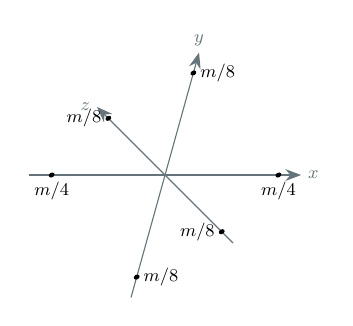
\begin{tikzpicture}[scale=0.72,transform shape]
\begin{scope}[x={(2cm,0cm)},y={(.5cm,1.8cm)},z={(-1cm,1cm)}]
\draw[axis] (-1.2,0,0)--(1.2,0,0) node[right] {$x$};\draw[axis] (0,-1.2,0)--(0,1.2,0) node[above] {$y$};\draw[axis] (0,0,-1.2)--(0,0,1.2) node[left] {$z$};
\foreach \s in {-1,1}{\fill (\s,0,0) circle(.025) node[below] {$m/4$};\fill (0,\s,0) circle(.025) node[right] {$m/8$};\fill (0,0,\s) circle(.025) node[left] {$m/8$};}\end{scope}\end{tikzpicture}
\figcaption{解图综四.1V6\quad 球壳三条直径端点的六个质量点投影，三惯量的和保持2mR平方}
\end{minipage}\end{center}
\Needspace{37\baselineskip}
\item \textbf{题设与求解。} 一般两平行轴相距$d$，由已知惯量确定的质心距离为$r_1,r_2$，求几何候选与唯一情形。取$P_2=(0,0),P_1=(0,d)$，两圆方程相减得\[
y_C=\frac{r_2^2-r_1^2+d^2}{2d},\qquad x_C=\pm\sqrt{r_2^2-y_C^2}.
\]
存在交点的条件是$|r_1-r_2|\leqslant d\leqslant r_1+r_2$；相切时根号为零，质心落在两轴连线上，两个候选合一。例如$d=2l,r_1=r_2=l$时$C=(0,l)$，到同一$P_3$的距离为$l$，故$I_3=I_C+ml^2$。图V7将相切两圆和唯一质心画出。
\begin{center}\begin{minipage}{.98\linewidth}\centering
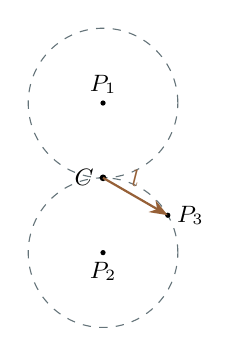
\begin{tikzpicture}[scale=0.95,transform shape]
\draw[guide] (0,0) circle(1);\draw[guide] (0,2) circle(1);
\fill (0,0) circle(.035) node[below] {$P_2$};\fill (0,2) circle(.035) node[above] {$P_1$};
\fill (0,1) circle(.045) node[left] {$C$};\fill (0.8660254037844386,.5) circle(.035) node[right] {$P_3$};
\draw[force] (0,1)--(0.8660254037844386,.5) node[midway,above] {$l$};\end{tikzpicture}
\figcaption{解图综四.1V7\quad 两距离圆相切时质心候选合一}
\end{minipage}\end{center}
\Needspace{37\baselineskip}
\item \textbf{题设与求解。} 对同一非均匀椭圆环，求垂直环面、过椭圆中心的转动惯量$J$及其范围。由垂轴定理$J=I_A+I_B$与主解关系，\[
J=mA^2+\left(1-\frac{A^2}{B^2}\right)I_A.
\]
每个质元有$0\leqslant y^2\leqslant B^2$，所以$0\leqslant I_A\leqslant mB^2$；当$A\geqslant B$时得到$mB^2\leqslant J\leqslant mA^2$。端值对应质量分别集中到短轴或长轴端点的极限。图V8取$A=2B$，画$J/(mB^2)=4-3I_A/(mB^2)$，同时保留任意线密度下的完整线性关系。
\begin{center}\begin{minipage}{.98\linewidth}\centering
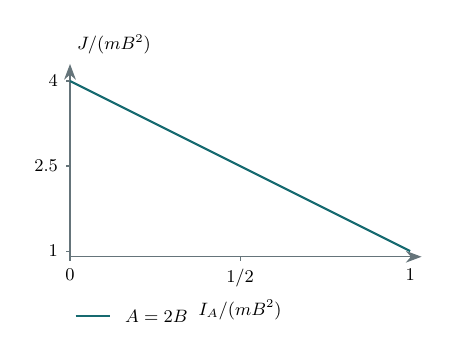
\begin{tikzpicture}[scale=0.72,transform shape]
\draw[axis] (0,0)--(6.2,0);\draw[axis] (0,0)--(0,3.4000000000000004);
\draw[thin,color=muted] (0.0000000,0)--(0.0000000,-.07);\node[below] at (0.0000000,-.09) {$0$};
\draw[thin,color=muted] (3.0000000,0)--(3.0000000,-.07);\node[below] at (3.0000000,-.09) {$1/2$};
\draw[thin,color=muted] (6.0000000,0)--(6.0000000,-.07);\node[below] at (6.0000000,-.09) {$1$};
\draw[thin,color=muted] (0,0.1000000)--(-.07,0.1000000);\node[left] at (-.09,0.1000000) {$1$};
\draw[thin,color=muted] (0,1.6000000)--(-.07,1.6000000);\node[left] at (-.09,1.6000000) {$2.5$};
\draw[thin,color=muted] (0,3.1000000)--(-.07,3.1000000);\node[left] at (-.09,3.1000000) {$4$};
\node[below] at (3.0,-.64) {$I_A/(mB^2)$};\node[above right] at (0,3.45) {$J/(mB^2)$};
\draw[traj] plot coordinates {(0.0000000,3.1000000) (0.0300000,3.0850000) (0.0600000,3.0700000) (0.0900000,3.0550000) (0.1200000,3.0400000) (0.1500000,3.0250000) (0.1800000,3.0100000) (0.2100000,2.9950000) (0.2400000,2.9800000) (0.2700000,2.9650000) (0.3000000,2.9500000) (0.3300000,2.9350000) (0.3600000,2.9200000) (0.3900000,2.9050000) (0.4200000,2.8900000) (0.4500000,2.8750000) (0.4800000,2.8600000) (0.5100000,2.8450000) (0.5400000,2.8300000) (0.5700000,2.8150000) (0.6000000,2.8000000) (0.6300000,2.7850000) (0.6600000,2.7700000) (0.6900000,2.7550000) (0.7200000,2.7400000) (0.7500000,2.7250000) (0.7800000,2.7100000) (0.8100000,2.6950000) (0.8400000,2.6800000) (0.8700000,2.6650000) (0.9000000,2.6500000) (0.9300000,2.6350000) (0.9600000,2.6200000) (0.9900000,2.6050000) (1.0200000,2.5900000) (1.0500000,2.5750000) (1.0800000,2.5600000) (1.1100000,2.5450000) (1.1400000,2.5300000) (1.1700000,2.5150000) (1.2000000,2.5000000) (1.2300000,2.4850000) (1.2600000,2.4700000) (1.2900000,2.4550000) (1.3200000,2.4400000) (1.3500000,2.4250000) (1.3800000,2.4100000) (1.4100000,2.3950000) (1.4400000,2.3800000) (1.4700000,2.3650000) (1.5000000,2.3500000) (1.5300000,2.3350000) (1.5600000,2.3200000) (1.5900000,2.3050000) (1.6200000,2.2900000) (1.6500000,2.2750000) (1.6800000,2.2600000) (1.7100000,2.2450000) (1.7400000,2.2300000) (1.7700000,2.2150000) (1.8000000,2.2000000) (1.8300000,2.1850000) (1.8600000,2.1700000) (1.8900000,2.1550000) (1.9200000,2.1400000) (1.9500000,2.1250000) (1.9800000,2.1100000) (2.0100000,2.0950000) (2.0400000,2.0800000) (2.0700000,2.0650000) (2.1000000,2.0500000) (2.1300000,2.0350000) (2.1600000,2.0200000) (2.1900000,2.0050000) (2.2200000,1.9900000) (2.2500000,1.9750000) (2.2800000,1.9600000) (2.3100000,1.9450000) (2.3400000,1.9300000) (2.3700000,1.9150000) (2.4000000,1.9000000) (2.4300000,1.8850000) (2.4600000,1.8700000) (2.4900000,1.8550000) (2.5200000,1.8400000) (2.5500000,1.8250000) (2.5800000,1.8100000) (2.6100000,1.7950000) (2.6400000,1.7800000) (2.6700000,1.7650000) (2.7000000,1.7500000) (2.7300000,1.7350000) (2.7600000,1.7200000) (2.7900000,1.7050000) (2.8200000,1.6900000) (2.8500000,1.6750000) (2.8800000,1.6600000) (2.9100000,1.6450000) (2.9400000,1.6300000) (2.9700000,1.6150000) (3.0000000,1.6000000) (3.0300000,1.5850000) (3.0600000,1.5700000) (3.0900000,1.5550000) (3.1200000,1.5400000) (3.1500000,1.5250000) (3.1800000,1.5100000) (3.2100000,1.4950000) (3.2400000,1.4800000) (3.2700000,1.4650000) (3.3000000,1.4500000) (3.3300000,1.4350000) (3.3600000,1.4200000) (3.3900000,1.4050000) (3.4200000,1.3900000) (3.4500000,1.3750000) (3.4800000,1.3600000) (3.5100000,1.3450000) (3.5400000,1.3300000) (3.5700000,1.3150000) (3.6000000,1.3000000) (3.6300000,1.2850000) (3.6600000,1.2700000) (3.6900000,1.2550000) (3.7200000,1.2400000) (3.7500000,1.2250000) (3.7800000,1.2100000) (3.8100000,1.1950000) (3.8400000,1.1800000) (3.8700000,1.1650000) (3.9000000,1.1500000) (3.9300000,1.1350000) (3.9600000,1.1200000) (3.9900000,1.1050000) (4.0200000,1.0900000) (4.0500000,1.0750000) (4.0800000,1.0600000) (4.1100000,1.0450000) (4.1400000,1.0300000) (4.1700000,1.0150000) (4.2000000,1.0000000) (4.2300000,0.9850000) (4.2600000,0.9700000) (4.2900000,0.9550000) (4.3200000,0.9400000) (4.3500000,0.9250000) (4.3800000,0.9100000) (4.4100000,0.8950000) (4.4400000,0.8800000) (4.4700000,0.8650000) (4.5000000,0.8500000) (4.5300000,0.8350000) (4.5600000,0.8200000) (4.5900000,0.8050000) (4.6200000,0.7900000) (4.6500000,0.7750000) (4.6800000,0.7600000) (4.7100000,0.7450000) (4.7400000,0.7300000) (4.7700000,0.7150000) (4.8000000,0.7000000) (4.8300000,0.6850000) (4.8600000,0.6700000) (4.8900000,0.6550000) (4.9200000,0.6400000) (4.9500000,0.6250000) (4.9800000,0.6100000) (5.0100000,0.5950000) (5.0400000,0.5800000) (5.0700000,0.5650000) (5.1000000,0.5500000) (5.1300000,0.5350000) (5.1600000,0.5200000) (5.1900000,0.5050000) (5.2200000,0.4900000) (5.2500000,0.4750000) (5.2800000,0.4600000) (5.3100000,0.4450000) (5.3400000,0.4300000) (5.3700000,0.4150000) (5.4000000,0.4000000) (5.4300000,0.3850000) (5.4600000,0.3700000) (5.4900000,0.3550000) (5.5200000,0.3400000) (5.5500000,0.3250000) (5.5800000,0.3100000) (5.6100000,0.2950000) (5.6400000,0.2800000) (5.6700000,0.2650000) (5.7000000,0.2500000) (5.7300000,0.2350000) (5.7600000,0.2200000) (5.7900000,0.2050000) (5.8200000,0.1900000) (5.8500000,0.1750000) (5.8800000,0.1600000) (5.9100000,0.1450000) (5.9400000,0.1300000) (5.9700000,0.1150000) (6.0000000,0.1000000)};
\draw[traj] (.1,-1.05)--(.7,-1.05);\node[right] at (.85,-1.05) {$A=2B$};\end{tikzpicture}
\figcaption{解图综四.1V8\quad 椭圆环垂直轴惯量与长轴惯量满足完整线性关系}
\end{minipage}\end{center}
\end{enumerate}

\Needspace{13\baselineskip}

\pdfbookmark[2]{第 2 题 方截面浮木的平衡与临界稳定性}{q2}

\section*{第 2 题\quad 方截面浮木的平衡与临界稳定性}\label{q:2}


一根均匀长方体木料，其正截面为边长$2a$的正方形，长边始终与水面平行。木料密度为$\rho$，水的密度为$\rho_0$，忽略毛细作用。

（1）给出木料部分露出水面时的平衡条件，说明浮心与重心的几何关系。

（2）木料对称地浮在水面上，正截面的一条对角线竖直，且只有一条长棱没入水中，浸截面是下角的等腰直角三角形。讨论这种姿态对微小转动的稳定性，尤其说明临界密度比时是否随遇平衡。必要的参数可自行定义。


\begin{center}\begin{minipage}{.98\linewidth}\centering
\begin{tikzpicture}[scale=.85,transform shape]

\fill[accent!12] (-1.05,-.364)--(0,-1.414)--(1.05,-.364)--cycle;

\draw[object] (0,-1.414)--(1.414,0)--(0,1.414)--(-1.414,0)--cycle;
\fill (0,0) circle (2pt) node[above right] {$O$};

\draw[axis] (-2,-.364)--(2,-.364) node[right] {水面};
\fill (0,-.714) circle (2pt) node[right] {$C$};
\draw[force] (0,-.714)--(0,.6) node[left] {浮力};
\draw[force,color=warm] (0,0)--(0,-1.3) node[right] {重力};
\node at (0,-2.2) {长边垂直纸面，正截面边长$2a$};

\end{tikzpicture}
\figcaption{图综四.2\quad 对称尖角向下的浮木，浮力作用线通过浸三角形重心。}
\end{minipage}\end{center}

\Needspace{8\baselineskip}

\pdfbookmark[3]{题型定位}{q2-h0}

\subsection*{题型定位}

自由升沉浮木的静水力矩与临界非线性稳定性。先用排水量使重力、浮力平衡，再在固定浸面积下比较浮心的横向移动；临界一阶项消失时保留三阶力矩，判定对称姿态仍为稳定。

\Needspace{8\baselineskip}

\pdfbookmark[3]{知识点}{q2-h1}

\subsection*{知识点}

阿基米德原理把浮力大小写成排开水的重力，作用线通过排水体积重心。均匀柱体可在垂直长边的正截面计算浮心。平动平衡固定$S=4a^2\rho/\rho_0$，力矩平衡另要求浮心与整体重心竖直共线。微倾过程中升沉调节保持$pq=t^2$，浮心为三角形重心$(p/3,q/3)$。局部恢复由$p+q-3a$的符号确定，临界点的能量领先项为正四次项。

\Needspace{8\baselineskip}

\pdfbookmark[3]{物理图像}{q2-h2}

\subsection*{物理图像}

解图综四.2A画对称的浸三角形，面积比给$t$。图B在木料侧边坐标中标出水线、实际竖直方向及浮心，力臂由浮心相对$O$的水平位移决定。图C把两个浸长放到抛物线上比较；固定乘积使临界两端位移不同。图D画三种密度下的完整静水力矩，正倾角处的负力矩指向对称姿态。

\Needspace{8\baselineskip}

\pdfbookmark[3]{解题入口}{q2-h3}

\subsection*{解题入口}

先算浸面积与对称浸长，同时保留$t<2a$以对应一条棱入水的三角形截面。微倾后固定乘积$pq=t^2$，再由三角形重心与水线法向量写角度关系或直接力矩。把二次函数差因式分解成$(p-q)[a-(p+q)/3]$，一般密度读线性符号，临界用面积约束及三阶展开。

\Needspace{8\baselineskip}

\pdfbookmark[3]{标准解法}{q2-h4}

\subsection*{标准解法}


图综四.2取垂直木料长边的截面。整体重心$O$在正方形中心，浸入水中的截面面积为$S$，其几何重心$C$是浮心在本截面的位置。水中静压随深度增加，木料各处压力的合力竖直向上；其大小等于排开水的重力。对于沿长边均匀的柱体，排水体积为$Sb$，浮心的截面坐标由面积一阶矩给出$S\boldsymbol r_C=\int_S\boldsymbol r\,\mathrm dA$。这将水压作用转成通过浸区几何重心的一个竖直力。若木料长为$b$，重力与浮力分别为$4a^2b\rho g$、$Sb\rho_0g$。

第（1）问，部分浸入要求$0<\rho<\rho_0$，平动平衡给
\[
\boxed{S=4a^2\frac{\rho}{\rho_0}}.
\]
重力过$O$、浮力过$C$，二者都竖直。绕$O$无力矩还要求
\[
\boxed{O,C\text{位于同一竖直线上}}.
\]
面积条件保证力的大小，竖直共线条件保证力矩；两项条件须同时满足。对于给定密度，木料的升沉先选出排水面积，随后对不同倾角比较浮心位置，才确定哪些姿态能静止。这个顺序也用于微倾后的稳定性分析：各比较状态先保持同一排水量，再看力矩如何改变倾角。均匀木料水上部分的截面积为$S'=4a^2-S$、重心为$C'$。以$O$作原点，质量加权关系为$S\boldsymbol r_C+S'\boldsymbol r_{C'}=0$，所以$C,O,C'$共线，且$S|OC|=S'|OC'|$。若这条线与实际竖直方向有夹角，两部分重力的合力仍过$O$，浮力则过$C$，留下一项浮力矩$M_B=F_Bx_C$，其中$x_C$是浮心相对于$O$的水平位移。令其为零便得到上面的竖直共线条件。力平衡单独决定排水量，力矩平衡再选择木料姿态；密度条件、排水面积条件和共线条件共同构成第（1）问的平衡要求。
\begin{center}\begin{minipage}{.98\linewidth}\centering
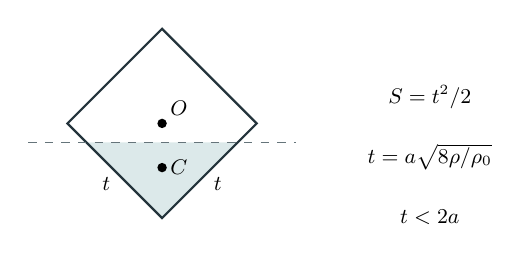
\begin{tikzpicture}[scale=.85,transform shape]

\fill[accent!15] (-1.131,-.283)--(0,-1.414)--(1.131,-.283)--cycle;

\draw[object] (0,-1.414)--(1.414,0)--(0,1.414)--(-1.414,0)--cycle;
\fill (0,0) circle (2pt) node[above right] {$O$};

\draw[guide] (-2,-.283)--(2,-.283);
\node[left] at (-.65,-.9) {$t$};\node[right] at (.65,-.9) {$t$};
\fill (0,-.66) circle (2pt) node[right] {$C$};
\node at (4, .4) {$S=t^2/2$};
\node at (4,-.5) {$t=a\sqrt{8\rho/\rho_0}$};
\node at (4,-1.4) {$t<2a$};

\end{tikzpicture}
\figcaption{解图综四.2A\quad 对称浸区是等腰直角三角形；面积比确定两边浸长。}
\end{minipage}\end{center}
第（2）问，解图综四.2A在对称姿态中令下角沿两边的浸长均为$t$，则
\[
S=\frac{t^2}{2},\qquad t=a\sqrt{\frac{8\rho}{\rho_0}},
\qquad 0<t<2a.
\]
最后一个条件等价于$0<\rho/\rho_0<1/2$，保证只有下方一条长棱浸水。现使木料微倾，并允许它少量升沉以维持浮力等于重力。两侧浸长改为$p,q$，且
\[
\boxed{pq=t^2}.
\]
微倾时木料可在竖直方向稍作平移，水线位置随姿态调节，使所排水的面积保持原值。两边仍相互垂直；在下角建立分别沿两木料侧边的正交坐标$x,y$，三角形顶点为$(0,0),(p,0),(0,q)$，水线为$x/p+y/q=1$。对该区域作面积积分，$\int_Sx\,\mathrm dA=Sp/3$、$\int_Sy\,\mathrm dA=Sq/3$，故浮心为$(p/3,q/3)$。正方形中心$O$在同一坐标中为$(a,a)$。
\begin{center}\begin{minipage}{.98\linewidth}\centering
\begin{tikzpicture}[scale=.85,transform shape]

\coordinate (V) at (0,0);\coordinate (U) at (1.2,0);\coordinate (W) at (0,1.875);
\fill[accent!15] (V)--(U)--(W)--cycle;
\draw[object] (0,0) rectangle (2,2);
\draw[traj] (U)--(W);
\fill (1,1) circle (2pt) node[below right] {$O$};
\fill (.4,.625) circle (2pt) node[left] {$C$};
\draw[guide] (1,1)--(.4,.625);
\draw[force] (.4,.625)--(1.411,1.272);
\draw[guide] (1.411,1.272)--(2.8,2.16096);
\node[above] at (2.8,2.16096) {浮力竖线};
\draw[guide] (1,1)--(1.9,1.576);
\node[below] at (.6,0) {$p$};\node[left] at (0,.94) {$q$};
\node[anchor=west,align=left] at (3.4,1.2) {$O=(a,a),\ C=(p/3,q/3)$\\$pq=t^2$\\$\tan\phi=p/q$\\$\tan\phi'=(a-q/3)/(a-p/3)$};
\node at (2.5,-1) {侧边坐标中水线斜置，竖直方向与水线垂直};

\end{tikzpicture}
\figcaption{解图综四.2B\quad 微倾后三角形浮心及实际竖直方向；本图用木料侧边作坐标。}
\end{minipage}\end{center}
解图综四.2B以一条侧边的法线为参照方向。设过$O$竖直线与该方向夹角为$\phi$，$OC$与同方向夹角为$\phi'$，按图的$p<q$一侧取正，几何关系给
\[
\tan\phi=\frac pq,\qquad
\tan\phi'=\frac{a-q/3}{a-p/3}.
\]
在未倾斜时$p=q=t$，两角相等。倾斜后若$\phi'<\phi$，浮心移到能提供恢复力矩的一侧，为稳定；若$\phi'>\phi$，力矩使扰动继续扩大，为不稳定。

由于$p,q<2a$，分母均为正。比较正切等价于比较
\[
\phi'<\phi
\ \Longleftrightarrow\
p\left(a-\frac p3\right)>
q\left(a-\frac q3\right).
\]
定义$G(z)=az-z^2/3$，它在$z=3a/2$处取最大值。更直接地，
\[
G(p)-G(q)=(p-q)\left(a-\frac{p+q}{3}\right).
\]
这个因式分解也给出浮力矩的具体表达。水线的向上单位法向量在木料坐标中为$\boldsymbol n=(q,p)/\sqrt{p^2+q^2}$，因此浮力为$F_B\boldsymbol n$。以逆时针转动为力矩正向，关于$O$的力矩为
\[
\begin{aligned}
\tau_O&=\frac{F_B}{\sqrt{p^2+q^2}}\left[
p\left(\frac p3-a\right)-q\left(\frac q3-a\right)\right]\\
&=\frac{F_B(p-q)(p+q-3a)}{3\sqrt{p^2+q^2}}
=-\frac{F_B[G(p)-G(q)]}{\sqrt{p^2+q^2}}.
\end{aligned}
\]
选倾转角$\delta$使$p<q$时$\delta>0$，恢复力矩为负。因$p-q<0$，恢复力矩的条件正是$p+q>3a$。解图综四.2D画出三种密度下力矩随倾角的变化，正倾角处的负力矩指向对称姿态，使浮心的角度比较与实际恢复方向对应。
\begin{center}\begin{minipage}{.98\linewidth}\centering
\begin{tikzpicture}[scale=0.72,transform shape]
\draw[axis] (0,0)--(6.2,0);\draw[axis] (0,0)--(0,3.4000000000000004);
\draw[thin,color=muted] (0.0000000,0)--(0.0000000,-.07);\node[below] at (0.0000000,-.09) {$-.15$};
\draw[thin,color=muted] (3.0000000,0)--(3.0000000,-.07);\node[below] at (3.0000000,-.09) {$0$};
\draw[thin,color=muted] (6.0000000,0)--(6.0000000,-.07);\node[below] at (6.0000000,-.09) {$.15$};
\draw[thin,color=muted] (0,0.5333333)--(-.07,0.5333333);\node[left] at (-.09,0.5333333) {$-.02$};
\draw[thin,color=muted] (0,1.6000000)--(-.07,1.6000000);\node[left] at (-.09,1.6000000) {$0$};
\draw[thin,color=muted] (0,2.6666667)--(-.07,2.6666667);\node[left] at (-.09,2.6666667) {$.02$};
\node[below] at (3.0,-.64) {实际倾转角$\delta$（弧度）};\node[above right] at (0,3.45) {$\tau/(F_Ba)$};
\draw[traj] plot coordinates {(0.0000000,1.0788683) (0.0200000,1.0806336) (0.0400000,1.0824345) (0.0600000,1.0842707) (0.0800000,1.0861418) (0.1000000,1.0880477) (0.1200000,1.0899881) (0.1400000,1.0919626) (0.1600000,1.0939710) (0.1800000,1.0960130) (0.2000000,1.0980884) (0.2200000,1.1001968) (0.2400000,1.1023380) (0.2600000,1.1045116) (0.2800000,1.1067176) (0.3000000,1.1089555) (0.3200000,1.1112251) (0.3400000,1.1135261) (0.3600000,1.1158582) (0.3800000,1.1182213) (0.4000000,1.1206149) (0.4200000,1.1230389) (0.4400000,1.1254930) (0.4600000,1.1279769) (0.4800000,1.1304904) (0.5000000,1.1330331) (0.5200000,1.1356049) (0.5400000,1.1382054) (0.5600000,1.1408345) (0.5800000,1.1434917) (0.6000000,1.1461770) (0.6200000,1.1488899) (0.6400000,1.1516304) (0.6600000,1.1543980) (0.6800000,1.1571926) (0.7000000,1.1600139) (0.7200000,1.1628616) (0.7400000,1.1657355) (0.7600000,1.1686353) (0.7800000,1.1715608) (0.8000000,1.1745117) (0.8200000,1.1774878) (0.8400000,1.1804888) (0.8600000,1.1835145) (0.8800000,1.1865645) (0.9000000,1.1896388) (0.9200000,1.1927369) (0.9400000,1.1958588) (0.9600000,1.1990040) (0.9800000,1.2021724) (1.0000000,1.2053638) (1.0200000,1.2085778) (1.0400000,1.2118142) (1.0600000,1.2150729) (1.0800000,1.2183535) (1.1000000,1.2216558) (1.1200000,1.2249795) (1.1400000,1.2283245) (1.1600000,1.2316904) (1.1800000,1.2350771) (1.2000000,1.2384843) (1.2200000,1.2419117) (1.2400000,1.2453591) (1.2600000,1.2488263) (1.2800000,1.2523131) (1.3000000,1.2558191) (1.3200000,1.2593442) (1.3400000,1.2628881) (1.3600000,1.2664506) (1.3800000,1.2700315) (1.4000000,1.2736304) (1.4200000,1.2772472) (1.4400000,1.2808817) (1.4600000,1.2845336) (1.4800000,1.2882026) (1.5000000,1.2918886) (1.5200000,1.2955913) (1.5400000,1.2993105) (1.5600000,1.3030459) (1.5800000,1.3067973) (1.6000000,1.3105645) (1.6200000,1.3143472) (1.6400000,1.3181452) (1.6600000,1.3219583) (1.6800000,1.3257863) (1.7000000,1.3296289) (1.7200000,1.3334859) (1.7400000,1.3373571) (1.7600000,1.3412422) (1.7800000,1.3451410) (1.8000000,1.3490533) (1.8200000,1.3529788) (1.8400000,1.3569174) (1.8600000,1.3608687) (1.8800000,1.3648327) (1.9000000,1.3688089) (1.9200000,1.3727973) (1.9400000,1.3767976) (1.9600000,1.3808096) (1.9800000,1.3848330) (2.0000000,1.3888676) (2.0200000,1.3929132) (2.0400000,1.3969696) (2.0600000,1.4010366) (2.0800000,1.4051138) (2.1000000,1.4092012) (2.1200000,1.4132984) (2.1400000,1.4174053) (2.1600000,1.4215216) (2.1800000,1.4256471) (2.2000000,1.4297816) (2.2200000,1.4339249) (2.2400000,1.4380767) (2.2600000,1.4422368) (2.2800000,1.4464051) (2.3000000,1.4505812) (2.3200000,1.4547649) (2.3400000,1.4589561) (2.3600000,1.4631545) (2.3800000,1.4673599) (2.4000000,1.4715721) (2.4200000,1.4757909) (2.4400000,1.4800159) (2.4600000,1.4842471) (2.4800000,1.4884842) (2.5000000,1.4927269) (2.5200000,1.4969751) (2.5400000,1.5012286) (2.5600000,1.5054870) (2.5800000,1.5097503) (2.6000000,1.5140181) (2.6200000,1.5182903) (2.6400000,1.5225666) (2.6600000,1.5268469) (2.6800000,1.5311308) (2.7000000,1.5354183) (2.7200000,1.5397090) (2.7400000,1.5440028) (2.7600000,1.5482993) (2.7800000,1.5525986) (2.8000000,1.5569002) (2.8200000,1.5612039) (2.8400000,1.5655097) (2.8600000,1.5698172) (2.8800000,1.5741262) (2.9000000,1.5784365) (2.9200000,1.5827479) (2.9400000,1.5870601) (2.9600000,1.5913731) (2.9800000,1.5956864) (3.0000000,1.6000000) (3.0200000,1.6043136) (3.0400000,1.6086269) (3.0600000,1.6129399) (3.0800000,1.6172521) (3.1000000,1.6215635) (3.1200000,1.6258738) (3.1400000,1.6301828) (3.1600000,1.6344903) (3.1800000,1.6387961) (3.2000000,1.6430998) (3.2200000,1.6474014) (3.2400000,1.6517007) (3.2600000,1.6559972) (3.2800000,1.6602910) (3.3000000,1.6645817) (3.3200000,1.6688692) (3.3400000,1.6731531) (3.3600000,1.6774334) (3.3800000,1.6817097) (3.4000000,1.6859819) (3.4200000,1.6902497) (3.4400000,1.6945130) (3.4600000,1.6987714) (3.4800000,1.7030249) (3.5000000,1.7072731) (3.5200000,1.7115158) (3.5400000,1.7157529) (3.5600000,1.7199841) (3.5800000,1.7242091) (3.6000000,1.7284279) (3.6200000,1.7326401) (3.6400000,1.7368455) (3.6600000,1.7410439) (3.6800000,1.7452351) (3.7000000,1.7494188) (3.7200000,1.7535949) (3.7400000,1.7577632) (3.7600000,1.7619233) (3.7800000,1.7660751) (3.8000000,1.7702184) (3.8200000,1.7743529) (3.8400000,1.7784784) (3.8600000,1.7825947) (3.8800000,1.7867016) (3.9000000,1.7907988) (3.9200000,1.7948862) (3.9400000,1.7989634) (3.9600000,1.8030304) (3.9800000,1.8070868) (4.0000000,1.8111324) (4.0200000,1.8151670) (4.0400000,1.8191904) (4.0600000,1.8232024) (4.0800000,1.8272027) (4.1000000,1.8311911) (4.1200000,1.8351673) (4.1400000,1.8391313) (4.1600000,1.8430826) (4.1800000,1.8470212) (4.2000000,1.8509467) (4.2200000,1.8548590) (4.2400000,1.8587578) (4.2600000,1.8626429) (4.2800000,1.8665141) (4.3000000,1.8703711) (4.3200000,1.8742137) (4.3400000,1.8780417) (4.3600000,1.8818548) (4.3800000,1.8856528) (4.4000000,1.8894355) (4.4200000,1.8932027) (4.4400000,1.8969541) (4.4600000,1.9006895) (4.4800000,1.9044087) (4.5000000,1.9081114) (4.5200000,1.9117974) (4.5400000,1.9154664) (4.5600000,1.9191183) (4.5800000,1.9227528) (4.6000000,1.9263696) (4.6200000,1.9299685) (4.6400000,1.9335494) (4.6600000,1.9371119) (4.6800000,1.9406558) (4.7000000,1.9441809) (4.7200000,1.9476869) (4.7400000,1.9511737) (4.7600000,1.9546409) (4.7800000,1.9580883) (4.8000000,1.9615157) (4.8200000,1.9649229) (4.8400000,1.9683096) (4.8600000,1.9716755) (4.8800000,1.9750205) (4.9000000,1.9783442) (4.9200000,1.9816465) (4.9400000,1.9849271) (4.9600000,1.9881858) (4.9800000,1.9914222) (5.0000000,1.9946362) (5.0200000,1.9978276) (5.0400000,2.0009960) (5.0600000,2.0041412) (5.0800000,2.0072631) (5.1000000,2.0103612) (5.1200000,2.0134355) (5.1400000,2.0164855) (5.1600000,2.0195112) (5.1800000,2.0225122) (5.2000000,2.0254883) (5.2200000,2.0284392) (5.2400000,2.0313647) (5.2600000,2.0342645) (5.2800000,2.0371384) (5.3000000,2.0399861) (5.3200000,2.0428074) (5.3400000,2.0456020) (5.3600000,2.0483696) (5.3800000,2.0511101) (5.4000000,2.0538230) (5.4200000,2.0565083) (5.4400000,2.0591655) (5.4600000,2.0617946) (5.4800000,2.0643951) (5.5000000,2.0669669) (5.5200000,2.0695096) (5.5400000,2.0720231) (5.5600000,2.0745070) (5.5800000,2.0769611) (5.6000000,2.0793851) (5.6200000,2.0817787) (5.6400000,2.0841418) (5.6600000,2.0864739) (5.6800000,2.0887749) (5.7000000,2.0910445) (5.7200000,2.0932824) (5.7400000,2.0954884) (5.7600000,2.0976620) (5.7800000,2.0998032) (5.8000000,2.1019116) (5.8200000,2.1039870) (5.8400000,2.1060290) (5.8600000,2.1080374) (5.8800000,2.1100119) (5.9000000,2.1119523) (5.9200000,2.1138582) (5.9400000,2.1157293) (5.9600000,2.1175655) (5.9800000,2.1193664) (6.0000000,2.1211317)};
\draw[traj] (.1,-1.05)--(.7,-1.05);\node[right] at (.85,-1.05) {密度比$1/4$};\draw[dashed,thick,color=warm] plot coordinates {(0.0000000,1.7309772) (0.0200000,1.7283253) (0.0400000,1.7257105) (0.0600000,1.7231325) (0.0800000,1.7205909) (0.1000000,1.7180855) (0.1200000,1.7156159) (0.1400000,1.7131820) (0.1600000,1.7107833) (0.1800000,1.7084196) (0.2000000,1.7060907) (0.2200000,1.7037961) (0.2400000,1.7015357) (0.2600000,1.6993092) (0.2800000,1.6971162) (0.3000000,1.6949565) (0.3200000,1.6928298) (0.3400000,1.6907359) (0.3600000,1.6886743) (0.3800000,1.6866449) (0.4000000,1.6846474) (0.4200000,1.6826815) (0.4400000,1.6807469) (0.4600000,1.6788433) (0.4800000,1.6769705) (0.5000000,1.6751282) (0.5200000,1.6733161) (0.5400000,1.6715340) (0.5600000,1.6697815) (0.5800000,1.6680584) (0.6000000,1.6663645) (0.6200000,1.6646994) (0.6400000,1.6630628) (0.6600000,1.6614546) (0.6800000,1.6598745) (0.7000000,1.6583221) (0.7200000,1.6567972) (0.7400000,1.6552996) (0.7600000,1.6538290) (0.7800000,1.6523851) (0.8000000,1.6509676) (0.8200000,1.6495764) (0.8400000,1.6482110) (0.8600000,1.6468714) (0.8800000,1.6455571) (0.9000000,1.6442680) (0.9200000,1.6430038) (0.9400000,1.6417642) (0.9600000,1.6405489) (0.9800000,1.6393578) (1.0000000,1.6381906) (1.0200000,1.6370469) (1.0400000,1.6359266) (1.0600000,1.6348293) (1.0800000,1.6337550) (1.1000000,1.6327031) (1.1200000,1.6316736) (1.1400000,1.6306662) (1.1600000,1.6296806) (1.1800000,1.6287166) (1.2000000,1.6277739) (1.2200000,1.6268523) (1.2400000,1.6259515) (1.2600000,1.6250712) (1.2800000,1.6242113) (1.3000000,1.6233714) (1.3200000,1.6225514) (1.3400000,1.6217510) (1.3600000,1.6209698) (1.3800000,1.6202078) (1.4000000,1.6194646) (1.4200000,1.6187400) (1.4400000,1.6180338) (1.4600000,1.6173456) (1.4800000,1.6166753) (1.5000000,1.6160227) (1.5200000,1.6153874) (1.5400000,1.6147692) (1.5600000,1.6141680) (1.5800000,1.6135833) (1.6000000,1.6130151) (1.6200000,1.6124631) (1.6400000,1.6119270) (1.6600000,1.6114065) (1.6800000,1.6109016) (1.7000000,1.6104118) (1.7200000,1.6099370) (1.7400000,1.6094769) (1.7600000,1.6090313) (1.7800000,1.6086000) (1.8000000,1.6081827) (1.8200000,1.6077792) (1.8400000,1.6073892) (1.8600000,1.6070126) (1.8800000,1.6066490) (1.9000000,1.6062982) (1.9200000,1.6059601) (1.9400000,1.6056343) (1.9600000,1.6053207) (1.9800000,1.6050189) (2.0000000,1.6047288) (2.0200000,1.6044502) (2.0400000,1.6041827) (2.0600000,1.6039263) (2.0800000,1.6036805) (2.1000000,1.6034453) (2.1200000,1.6032203) (2.1400000,1.6030053) (2.1600000,1.6028002) (2.1800000,1.6026046) (2.2000000,1.6024184) (2.2200000,1.6022413) (2.2400000,1.6020731) (2.2600000,1.6019135) (2.2800000,1.6017624) (2.3000000,1.6016194) (2.3200000,1.6014844) (2.3400000,1.6013571) (2.3600000,1.6012373) (2.3800000,1.6011248) (2.4000000,1.6010194) (2.4200000,1.6009207) (2.4400000,1.6008287) (2.4600000,1.6007430) (2.4800000,1.6006634) (2.5000000,1.6005897) (2.5200000,1.6005217) (2.5400000,1.6004591) (2.5600000,1.6004018) (2.5800000,1.6003494) (2.6000000,1.6003018) (2.6200000,1.6002588) (2.6400000,1.6002200) (2.6600000,1.6001853) (2.6800000,1.6001545) (2.7000000,1.6001273) (2.7200000,1.6001035) (2.7400000,1.6000829) (2.7600000,1.6000652) (2.7800000,1.6000502) (2.8000000,1.6000377) (2.8200000,1.6000275) (2.8400000,1.6000193) (2.8600000,1.6000129) (2.8800000,1.6000081) (2.9000000,1.6000047) (2.9200000,1.6000024) (2.9400000,1.6000010) (2.9600000,1.6000003) (2.9800000,1.6000000) (3.0000000,1.6000000) (3.0200000,1.6000000) (3.0400000,1.5999997) (3.0600000,1.5999990) (3.0800000,1.5999976) (3.1000000,1.5999953) (3.1200000,1.5999919) (3.1400000,1.5999871) (3.1600000,1.5999807) (3.1800000,1.5999725) (3.2000000,1.5999623) (3.2200000,1.5999498) (3.2400000,1.5999348) (3.2600000,1.5999171) (3.2800000,1.5998965) (3.3000000,1.5998727) (3.3200000,1.5998455) (3.3400000,1.5998147) (3.3600000,1.5997800) (3.3800000,1.5997412) (3.4000000,1.5996982) (3.4200000,1.5996506) (3.4400000,1.5995982) (3.4600000,1.5995409) (3.4800000,1.5994783) (3.5000000,1.5994103) (3.5200000,1.5993366) (3.5400000,1.5992570) (3.5600000,1.5991713) (3.5800000,1.5990793) (3.6000000,1.5989806) (3.6200000,1.5988752) (3.6400000,1.5987627) (3.6600000,1.5986429) (3.6800000,1.5985156) (3.7000000,1.5983806) (3.7200000,1.5982376) (3.7400000,1.5980865) (3.7600000,1.5979269) (3.7800000,1.5977587) (3.8000000,1.5975816) (3.8200000,1.5973954) (3.8400000,1.5971998) (3.8600000,1.5969947) (3.8800000,1.5967797) (3.9000000,1.5965547) (3.9200000,1.5963195) (3.9400000,1.5960737) (3.9600000,1.5958173) (3.9800000,1.5955498) (4.0000000,1.5952712) (4.0200000,1.5949811) (4.0400000,1.5946793) (4.0600000,1.5943657) (4.0800000,1.5940399) (4.1000000,1.5937018) (4.1200000,1.5933510) (4.1400000,1.5929874) (4.1600000,1.5926108) (4.1800000,1.5922208) (4.2000000,1.5918173) (4.2200000,1.5914000) (4.2400000,1.5909687) (4.2600000,1.5905231) (4.2800000,1.5900630) (4.3000000,1.5895882) (4.3200000,1.5890984) (4.3400000,1.5885935) (4.3600000,1.5880730) (4.3800000,1.5875369) (4.4000000,1.5869849) (4.4200000,1.5864167) (4.4400000,1.5858320) (4.4600000,1.5852308) (4.4800000,1.5846126) (4.5000000,1.5839773) (4.5200000,1.5833247) (4.5400000,1.5826544) (4.5600000,1.5819662) (4.5800000,1.5812600) (4.6000000,1.5805354) (4.6200000,1.5797922) (4.6400000,1.5790302) (4.6600000,1.5782490) (4.6800000,1.5774486) (4.7000000,1.5766286) (4.7200000,1.5757887) (4.7400000,1.5749288) (4.7600000,1.5740485) (4.7800000,1.5731477) (4.8000000,1.5722261) (4.8200000,1.5712834) (4.8400000,1.5703194) (4.8600000,1.5693338) (4.8800000,1.5683264) (4.9000000,1.5672969) (4.9200000,1.5662450) (4.9400000,1.5651707) (4.9600000,1.5640734) (4.9800000,1.5629531) (5.0000000,1.5618094) (5.0200000,1.5606422) (5.0400000,1.5594511) (5.0600000,1.5582358) (5.0800000,1.5569962) (5.1000000,1.5557320) (5.1200000,1.5544429) (5.1400000,1.5531286) (5.1600000,1.5517890) (5.1800000,1.5504236) (5.2000000,1.5490324) (5.2200000,1.5476149) (5.2400000,1.5461710) (5.2600000,1.5447004) (5.2800000,1.5432028) (5.3000000,1.5416779) (5.3200000,1.5401255) (5.3400000,1.5385454) (5.3600000,1.5369372) (5.3800000,1.5353006) (5.4000000,1.5336355) (5.4200000,1.5319416) (5.4400000,1.5302185) (5.4600000,1.5284660) (5.4800000,1.5266839) (5.5000000,1.5248718) (5.5200000,1.5230295) (5.5400000,1.5211567) (5.5600000,1.5192531) (5.5800000,1.5173185) (5.6000000,1.5153526) (5.6200000,1.5133551) (5.6400000,1.5113257) (5.6600000,1.5092641) (5.6800000,1.5071702) (5.7000000,1.5050435) (5.7200000,1.5028838) (5.7400000,1.5006908) (5.7600000,1.4984643) (5.7800000,1.4962039) (5.8000000,1.4939093) (5.8200000,1.4915804) (5.8400000,1.4892167) (5.8600000,1.4868180) (5.8800000,1.4843841) (5.9000000,1.4819145) (5.9200000,1.4794091) (5.9400000,1.4768675) (5.9600000,1.4742895) (5.9800000,1.4716747) (6.0000000,1.4690228)};
\draw[dashed,thick,color=warm] (.1,-1.48)--(.7,-1.48);\node[right] at (.85,-1.48) {密度比$9/32$};\draw[dotted,thick,color=muted] plot coordinates {(0.0000000,2.7419297) (0.0200000,2.7324301) (0.0400000,2.7229697) (0.0600000,2.7135484) (0.0800000,2.7041658) (0.1000000,2.6948216) (0.1200000,2.6855154) (0.1400000,2.6762471) (0.1600000,2.6670162) (0.1800000,2.6578225) (0.2000000,2.6486657) (0.2200000,2.6395453) (0.2400000,2.6304612) (0.2600000,2.6214131) (0.2800000,2.6124006) (0.3000000,2.6034234) (0.3200000,2.5944812) (0.3400000,2.5855738) (0.3600000,2.5767007) (0.3800000,2.5678618) (0.4000000,2.5590568) (0.4200000,2.5502852) (0.4400000,2.5415469) (0.4600000,2.5328416) (0.4800000,2.5241688) (0.5000000,2.5155285) (0.5200000,2.5069202) (0.5400000,2.4983436) (0.5600000,2.4897986) (0.5800000,2.4812847) (0.6000000,2.4728017) (0.6200000,2.4643494) (0.6400000,2.4559273) (0.6600000,2.4475353) (0.6800000,2.4391731) (0.7000000,2.4308403) (0.7200000,2.4225367) (0.7400000,2.4142620) (0.7600000,2.4060160) (0.7800000,2.3977983) (0.8000000,2.3896086) (0.8200000,2.3814467) (0.8400000,2.3733123) (0.8600000,2.3652052) (0.8800000,2.3571250) (0.9000000,2.3490714) (0.9200000,2.3410443) (0.9400000,2.3330432) (0.9600000,2.3250681) (0.9800000,2.3171184) (1.0000000,2.3091941) (1.0200000,2.3012948) (1.0400000,2.2934203) (1.0600000,2.2855702) (1.0800000,2.2777443) (1.1000000,2.2699424) (1.1200000,2.2621642) (1.1400000,2.2544093) (1.1600000,2.2466776) (1.1800000,2.2389688) (1.2000000,2.2312826) (1.2200000,2.2236187) (1.2400000,2.2159768) (1.2600000,2.2083568) (1.2800000,2.2007583) (1.3000000,2.1931811) (1.3200000,2.1856250) (1.3400000,2.1780895) (1.3600000,2.1705746) (1.3800000,2.1630799) (1.4000000,2.1556051) (1.4200000,2.1481501) (1.4400000,2.1407145) (1.4600000,2.1332981) (1.4800000,2.1259006) (1.5000000,2.1185218) (1.5200000,2.1111614) (1.5400000,2.1038192) (1.5600000,2.0964949) (1.5800000,2.0891882) (1.6000000,2.0818989) (1.6200000,2.0746268) (1.6400000,2.0673715) (1.6600000,2.0601328) (1.6800000,2.0529105) (1.7000000,2.0457044) (1.7200000,2.0385141) (1.7400000,2.0313394) (1.7600000,2.0241800) (1.7800000,2.0170358) (1.8000000,2.0099064) (1.8200000,2.0027916) (1.8400000,1.9956912) (1.8600000,1.9886049) (1.8800000,1.9815324) (1.9000000,1.9744736) (1.9200000,1.9674280) (1.9400000,1.9603956) (1.9600000,1.9533761) (1.9800000,1.9463691) (2.0000000,1.9393745) (2.0200000,1.9323921) (2.0400000,1.9254215) (2.0600000,1.9184625) (2.0800000,1.9115148) (2.1000000,1.9045783) (2.1200000,1.8976527) (2.1400000,1.8907377) (2.1600000,1.8838331) (2.1800000,1.8769387) (2.2000000,1.8700541) (2.2200000,1.8631792) (2.2400000,1.8563137) (2.2600000,1.8494574) (2.2800000,1.8426100) (2.3000000,1.8357712) (2.3200000,1.8289409) (2.3400000,1.8221188) (2.3600000,1.8153046) (2.3800000,1.8084981) (2.4000000,1.8016991) (2.4200000,1.7949073) (2.4400000,1.7881225) (2.4600000,1.7813444) (2.4800000,1.7745728) (2.5000000,1.7678075) (2.5200000,1.7610481) (2.5400000,1.7542945) (2.5600000,1.7475465) (2.5800000,1.7408037) (2.6000000,1.7340660) (2.6200000,1.7273331) (2.6400000,1.7206047) (2.6600000,1.7138807) (2.6800000,1.7071607) (2.7000000,1.7004446) (2.7200000,1.6937320) (2.7400000,1.6870229) (2.7600000,1.6803168) (2.7800000,1.6736136) (2.8000000,1.6669131) (2.8200000,1.6602150) (2.8400000,1.6535190) (2.8600000,1.6468249) (2.8800000,1.6401325) (2.9000000,1.6334416) (2.9200000,1.6267518) (2.9400000,1.6200630) (2.9600000,1.6133749) (2.9800000,1.6066874) (3.0000000,1.6000000) (3.0200000,1.5933126) (3.0400000,1.5866251) (3.0600000,1.5799370) (3.0800000,1.5732482) (3.1000000,1.5665584) (3.1200000,1.5598675) (3.1400000,1.5531751) (3.1600000,1.5464810) (3.1800000,1.5397850) (3.2000000,1.5330869) (3.2200000,1.5263864) (3.2400000,1.5196832) (3.2600000,1.5129771) (3.2800000,1.5062680) (3.3000000,1.4995554) (3.3200000,1.4928393) (3.3400000,1.4861193) (3.3600000,1.4793953) (3.3800000,1.4726669) (3.4000000,1.4659340) (3.4200000,1.4591963) (3.4400000,1.4524535) (3.4600000,1.4457055) (3.4800000,1.4389519) (3.5000000,1.4321925) (3.5200000,1.4254272) (3.5400000,1.4186556) (3.5600000,1.4118775) (3.5800000,1.4050927) (3.6000000,1.3983009) (3.6200000,1.3915019) (3.6400000,1.3846954) (3.6600000,1.3778812) (3.6800000,1.3710591) (3.7000000,1.3642288) (3.7200000,1.3573900) (3.7400000,1.3505426) (3.7600000,1.3436863) (3.7800000,1.3368208) (3.8000000,1.3299459) (3.8200000,1.3230613) (3.8400000,1.3161669) (3.8600000,1.3092623) (3.8800000,1.3023473) (3.9000000,1.2954217) (3.9200000,1.2884852) (3.9400000,1.2815375) (3.9600000,1.2745785) (3.9800000,1.2676079) (4.0000000,1.2606255) (4.0200000,1.2536309) (4.0400000,1.2466239) (4.0600000,1.2396044) (4.0800000,1.2325720) (4.1000000,1.2255264) (4.1200000,1.2184676) (4.1400000,1.2113951) (4.1600000,1.2043088) (4.1800000,1.1972084) (4.2000000,1.1900936) (4.2200000,1.1829642) (4.2400000,1.1758200) (4.2600000,1.1686606) (4.2800000,1.1614859) (4.3000000,1.1542956) (4.3200000,1.1470895) (4.3400000,1.1398672) (4.3600000,1.1326285) (4.3800000,1.1253732) (4.4000000,1.1181011) (4.4200000,1.1108118) (4.4400000,1.1035051) (4.4600000,1.0961808) (4.4800000,1.0888386) (4.5000000,1.0814782) (4.5200000,1.0740994) (4.5400000,1.0667019) (4.5600000,1.0592855) (4.5800000,1.0518499) (4.6000000,1.0443949) (4.6200000,1.0369201) (4.6400000,1.0294254) (4.6600000,1.0219105) (4.6800000,1.0143750) (4.7000000,1.0068189) (4.7200000,0.9992417) (4.7400000,0.9916432) (4.7600000,0.9840232) (4.7800000,0.9763813) (4.8000000,0.9687174) (4.8200000,0.9610312) (4.8400000,0.9533224) (4.8600000,0.9455907) (4.8800000,0.9378358) (4.9000000,0.9300576) (4.9200000,0.9222557) (4.9400000,0.9144298) (4.9600000,0.9065797) (4.9800000,0.8987052) (5.0000000,0.8908059) (5.0200000,0.8828816) (5.0400000,0.8749319) (5.0600000,0.8669568) (5.0800000,0.8589557) (5.1000000,0.8509286) (5.1200000,0.8428750) (5.1400000,0.8347948) (5.1600000,0.8266877) (5.1800000,0.8185533) (5.2000000,0.8103914) (5.2200000,0.8022017) (5.2400000,0.7939840) (5.2600000,0.7857380) (5.2800000,0.7774633) (5.3000000,0.7691597) (5.3200000,0.7608269) (5.3400000,0.7524647) (5.3600000,0.7440727) (5.3800000,0.7356506) (5.4000000,0.7271983) (5.4200000,0.7187153) (5.4400000,0.7102014) (5.4600000,0.7016564) (5.4800000,0.6930798) (5.5000000,0.6844715) (5.5200000,0.6758312) (5.5400000,0.6671584) (5.5600000,0.6584531) (5.5800000,0.6497148) (5.6000000,0.6409432) (5.6200000,0.6321382) (5.6400000,0.6232993) (5.6600000,0.6144262) (5.6800000,0.6055188) (5.7000000,0.5965766) (5.7200000,0.5875994) (5.7400000,0.5785869) (5.7600000,0.5695388) (5.7800000,0.5604547) (5.8000000,0.5513343) (5.8200000,0.5421775) (5.8400000,0.5329838) (5.8600000,0.5237529) (5.8800000,0.5144846) (5.9000000,0.5051784) (5.9200000,0.4958342) (5.9400000,0.4864516) (5.9600000,0.4770303) (5.9800000,0.4675699) (6.0000000,0.4580703)};
\draw[dotted,thick,color=muted] (.1,-1.9100000000000001)--(.7,-1.9100000000000001);\node[right] at (.85,-1.9100000000000001) {密度比$1/3$};\end{tikzpicture}
\figcaption{解图综四.2D\quad 正角处负力矩恢复到对称姿态，临界曲线的领先项为三次}
\end{minipage}\end{center}
\begin{center}\begin{minipage}{.98\linewidth}\centering
\begin{tikzpicture}[scale=.85,transform shape]

\draw[axis] (0,0)--(6.5,0) node[right] {$z/a$};
\draw[axis] (0,0)--(0,3.2) node[above] {$G(z)/a^2$};
\draw[traj,domain=0:2.8,samples=100] plot ({2*\x},{3*(\x-\x*\x/3)});
\draw[guide] (3,0)--(3,2.25);
\node[below] at (3,0) {$3/2$};
\node at (4.8,3) {$G(z)=az-z^2/3$};
\node at (3,-1) {$G(p)-G(q)=(p-q)[a-(p+q)/3]$};
\node at (3,-2) {临界时$pq=(3a/2)^2$且$p+q>3a$，仍有恢复力};

\end{tikzpicture}
\figcaption{解图综四.2C\quad 抛物线判据与临界的固定面积约束，三阶项决定临界处的恢复力矩。}
\end{minipage}\end{center}
解图综四.2C比较抛物线上两点。若$t>3a/2$，任意足够小倾斜仍有$p+q>3a$，稳定；若$t<3a/2$，小倾斜后仍有$p+q<3a$，不稳定。临界$t=3a/2$时，一阶恢复系数为零，固定面积约束下的高阶浮心移动决定恢复方向。因为$pq=t^2$固定且$p\ne q$，算术几何平均不等式给
\[
p+q>2\sqrt{pq}=3a,
\]
也可按抛物线的左右位移理解这一结论。设$p=t-\Delta p$，由面积保持得$q=t^2/(t-\Delta p)=t+\Delta q$，其中$\Delta q=t\Delta p/(t-\Delta p)>\Delta p$。在临界$t=3a/2$处，抛物线关于顶点对称，右侧较大的位移使$G(q)$更低，于是$G(p)>G(q)$。所以临界处仍有恢复力矩，只是领先阶较高，它也是稳定平衡。

将$t=a\sqrt{8\rho/\rho_0}$代入，结论为
\[
\boxed{\begin{array}{ll}
0<\rho/\rho_0<9/32:&\text{不稳定},\\
9/32\le\rho/\rho_0<1/2:&\text{稳定}.
\end{array}}
\]
还可令$p=t e^{-\varepsilon},q=t e^\varepsilon$，把面积约束精确保留。在临界$t=3a/2$处，
\[
G(p)-G(q)
=(-2t\sinh\varepsilon)
\left[a-\frac{2t\cosh\varepsilon}{3}\right]
=2at\sinh\varepsilon(\cosh\varepsilon-1)
\sim at\,\varepsilon^3>0.
\]
由力矩式还可定出这一高阶量的物理系数。此时$\sqrt{p^2+q^2}\simeq\sqrt2t$，因此$\tau_O\simeq-F_Ba\varepsilon^3/\sqrt2$。实际倾转角满足$\delta=\arctan(q/p)-\pi/4=\arctan(e^{2\varepsilon})-\pi/4=\varepsilon+O(\varepsilon^3)$，故领先恢复力矩也写成$-F_Ba\delta^3/\sqrt2$。由解图综四.2C 的对称点出发，沿保持浸面积不变的路径积分 $\mathrm dU=-\tau_O\,\mathrm d\delta$，得到
\[
U(\delta)-U(0)=\frac{F_Ba}{4\sqrt2}\,\delta^4+o(\delta^4).
\]
临界时，一阶刚度为零；向左右任一侧微倾，四阶项都使势能增大，因此对称姿态仍是局部极小。上面取的是$p<q$的一侧；关于竖直对角线作镜像时，$p,q$互换，力矩随之反号，倾转角也反号，所以两侧扰动都受到指向对称姿态的恢复作用。

例如密度比为$1/4$时$t=\sqrt2a$，位于临界浸长以下，对称尖角姿态受扰后继续偏转；密度比为$1/3$时$t=\sqrt{8/3}a$，已经超过$3a/2$而仍小于$2a$，恢复力矩使木料回向对称姿态。

线性项也能用稳心高度解释。对称水线宽$w=\sqrt2t$，单位木料长度的水线二次矩为$w^3/12$，除以浸面积$S=t^2/2$得$BM=\sqrt2t/3$。浮心到重心的竖直距离为$BG=\sqrt2(a-t/3)$，因而$GM=BM-BG=\sqrt2(2t/3-a)$。小角浮力矩的一阶项为$-F_BGM\,\delta$，在$t>3a/2$时为恢复项，在$t<3a/2$时使扰动增大；临界点按上面的三阶项判定。以上局部扰动始终保持$p,q<2a$和三角形浸区。水线继续移动而碰到其他棱时，排水截面变为另一多边形，其浮心再按对应几何求取。


\Needspace{8\baselineskip}

\pdfbookmark[3]{关键洞察}{q2-h5}

\subsection*{关键洞察}

临界处$p+q$在倾斜后严格大于$2\sqrt{pq}=3a$，恢复力矩仍存在，领先为$-F_Ba\delta^3/\sqrt2$。线性稳心高$GM=\sqrt2(2t/3-a)$在此为零，对应线性频率为零；高阶势能保持局部最小。局部分析在同一三角形浸区内进行，水线碰到另一棱后按新的排水多边形求浮心。

\Needspace{8\baselineskip}

\pdfbookmark[3]{易错点}{q2-h6}

\subsection*{易错点}

密度低于水保证可能部分浸入，平衡还同时满足排水量与竖直共线。微倾时允许木料升沉并保持浸面积；$p=t-\Delta,q=t+\Delta$只是一阶写法，精确约束为乘积固定。临界比较用这一精确约束保留较高阶项。给定只有一条棱浸没，使密度比上限为$1/2$；临界$9/32$由本姿态的几何与浮心共同确定。

\Needspace{8\baselineskip}

\pdfbookmark[3]{课堂讲解建议}{q2-h7}

\subsection*{课堂讲解建议}

先分别画重力和浮力，解释大小相等与作用线共线各解决什么，再用微倾图指明浮力矩转向。令学生从固定乘积算一组$p,q$，追问两者之和是否仍为$2t$；由$pq=t^2$及$p\ne q$得$p+q>2t$，再比较抛物线函数值。到临界时追问一阶线性模型省去了哪一项，学生回答三阶恢复力矩；同时画线性零项和三阶力矩，再问能量在两侧怎样增加，用正四次势能项说明。最后用水线宽与浮心高计算$GM$，把线性方法与临界高阶结论放在同一图中理解。

\Needspace{8\baselineskip}

\pdfbookmark[3]{变式训练}{q2-h8}

\subsection*{变式训练}

\begin{enumerate}
\Needspace{37\baselineskip}
\item \textbf{题设与求解。} 比较密度比$1/4$与$1/3$时的尖角姿态。第一种$t/a=\sqrt2<3/2$，正倾角引起同向力矩，对称姿态不稳定；第二种$t/a=\sqrt{8/3}>3/2$且小于2，正倾角下力矩为负，姿态稳定。解图综四.2V1直接画两种完整力矩随小倾角的变化，符号分别对应扰动增大与恢复。
\begin{center}\begin{minipage}{.98\linewidth}\centering
\begin{tikzpicture}[scale=0.72,transform shape]
\draw[axis] (0,0)--(6.2,0);\draw[axis] (0,0)--(0,3.4000000000000004);
\draw[thin,color=muted] (0.0000000,0)--(0.0000000,-.07);\node[below] at (0.0000000,-.09) {$-.1$};
\draw[thin,color=muted] (3.0000000,0)--(3.0000000,-.07);\node[below] at (3.0000000,-.09) {$0$};
\draw[thin,color=muted] (6.0000000,0)--(6.0000000,-.07);\node[below] at (6.0000000,-.09) {$.1$};
\draw[thin,color=muted] (0,0.6000000)--(-.07,0.6000000);\node[left] at (-.09,0.6000000) {$-.01$};
\draw[thin,color=muted] (0,1.6000000)--(-.07,1.6000000);\node[left] at (-.09,1.6000000) {$0$};
\draw[thin,color=muted] (0,2.6000000)--(-.07,2.6000000);\node[left] at (-.09,2.6000000) {$.01$};
\node[below] at (3.0,-.64) {$\delta$（弧度）};\node[above right] at (0,3.45) {$\tau/(F_Ba)$};
\draw[traj] plot coordinates {(0.0000000,0.8600570) (0.0300000,0.8660833) (0.0600000,0.8721517) (0.0900000,0.8782617) (0.1200000,0.8844128) (0.1500000,0.8906046) (0.1800000,0.8968366) (0.2100000,0.9031084) (0.2400000,0.9094196) (0.2700000,0.9157696) (0.3000000,0.9221580) (0.3300000,0.9285845) (0.3600000,0.9350484) (0.3900000,0.9415494) (0.4200000,0.9480870) (0.4500000,0.9546609) (0.4800000,0.9612704) (0.5100000,0.9679152) (0.5400000,0.9745949) (0.5700000,0.9813090) (0.6000000,0.9880570) (0.6300000,0.9948386) (0.6600000,1.0016532) (0.6900000,1.0085005) (0.7200000,1.0153799) (0.7500000,1.0222912) (0.7800000,1.0292337) (0.8100000,1.0362071) (0.8400000,1.0432110) (0.8700000,1.0502449) (0.9000000,1.0573084) (0.9300000,1.0644010) (0.9600000,1.0715223) (0.9900000,1.0786719) (1.0200000,1.0858494) (1.0500000,1.0930542) (1.0800000,1.1002861) (1.1100000,1.1075445) (1.1400000,1.1148291) (1.1700000,1.1221393) (1.2000000,1.1294749) (1.2300000,1.1368353) (1.2600000,1.1442201) (1.2900000,1.1516289) (1.3200000,1.1590612) (1.3500000,1.1665168) (1.3800000,1.1739950) (1.4100000,1.1814956) (1.4400000,1.1890180) (1.4700000,1.1965619) (1.5000000,1.2041268) (1.5300000,1.2117123) (1.5600000,1.2193181) (1.5900000,1.2269436) (1.6200000,1.2345884) (1.6500000,1.2422522) (1.6800000,1.2499345) (1.7100000,1.2576349) (1.7400000,1.2653530) (1.7700000,1.2730884) (1.8000000,1.2808406) (1.8300000,1.2886092) (1.8600000,1.2963938) (1.8900000,1.3041941) (1.9200000,1.3120095) (1.9500000,1.3198397) (1.9800000,1.3276843) (2.0100000,1.3355428) (2.0400000,1.3434148) (2.0700000,1.3512999) (2.1000000,1.3591977) (2.1300000,1.3671079) (2.1600000,1.3750299) (2.1900000,1.3829633) (2.2200000,1.3909078) (2.2500000,1.3988630) (2.2800000,1.4068283) (2.3100000,1.4148035) (2.3400000,1.4227881) (2.3700000,1.4307817) (2.4000000,1.4387839) (2.4300000,1.4467943) (2.4600000,1.4548124) (2.4900000,1.4628379) (2.5200000,1.4708703) (2.5500000,1.4789093) (2.5800000,1.4869544) (2.6100000,1.4950052) (2.6400000,1.5030613) (2.6700000,1.5111223) (2.7000000,1.5191878) (2.7300000,1.5272574) (2.7600000,1.5353306) (2.7900000,1.5434072) (2.8200000,1.5514866) (2.8500000,1.5595684) (2.8800000,1.5676523) (2.9100000,1.5757378) (2.9400000,1.5838245) (2.9700000,1.5919120) (3.0000000,1.6000000) (3.0300000,1.6080880) (3.0600000,1.6161755) (3.0900000,1.6242622) (3.1200000,1.6323477) (3.1500000,1.6404316) (3.1800000,1.6485134) (3.2100000,1.6565928) (3.2400000,1.6646694) (3.2700000,1.6727426) (3.3000000,1.6808122) (3.3300000,1.6888777) (3.3600000,1.6969387) (3.3900000,1.7049948) (3.4200000,1.7130456) (3.4500000,1.7210907) (3.4800000,1.7291297) (3.5100000,1.7371621) (3.5400000,1.7451876) (3.5700000,1.7532057) (3.6000000,1.7612161) (3.6300000,1.7692183) (3.6600000,1.7772119) (3.6900000,1.7851965) (3.7200000,1.7931717) (3.7500000,1.8011370) (3.7800000,1.8090922) (3.8100000,1.8170367) (3.8400000,1.8249701) (3.8700000,1.8328921) (3.9000000,1.8408023) (3.9300000,1.8487001) (3.9600000,1.8565852) (3.9900000,1.8644572) (4.0200000,1.8723157) (4.0500000,1.8801603) (4.0800000,1.8879905) (4.1100000,1.8958059) (4.1400000,1.9036062) (4.1700000,1.9113908) (4.2000000,1.9191594) (4.2300000,1.9269116) (4.2600000,1.9346470) (4.2900000,1.9423651) (4.3200000,1.9500655) (4.3500000,1.9577478) (4.3800000,1.9654116) (4.4100000,1.9730564) (4.4400000,1.9806819) (4.4700000,1.9882877) (4.5000000,1.9958732) (4.5300000,2.0034381) (4.5600000,2.0109820) (4.5900000,2.0185044) (4.6200000,2.0260050) (4.6500000,2.0334832) (4.6800000,2.0409388) (4.7100000,2.0483711) (4.7400000,2.0557799) (4.7700000,2.0631647) (4.8000000,2.0705251) (4.8300000,2.0778607) (4.8600000,2.0851709) (4.8900000,2.0924555) (4.9200000,2.0997139) (4.9500000,2.1069458) (4.9800000,2.1141506) (5.0100000,2.1213281) (5.0400000,2.1284777) (5.0700000,2.1355990) (5.1000000,2.1426916) (5.1300000,2.1497551) (5.1600000,2.1567890) (5.1900000,2.1637929) (5.2200000,2.1707663) (5.2500000,2.1777088) (5.2800000,2.1846201) (5.3100000,2.1914995) (5.3400000,2.1983468) (5.3700000,2.2051614) (5.4000000,2.2119430) (5.4300000,2.2186910) (5.4600000,2.2254051) (5.4900000,2.2320848) (5.5200000,2.2387296) (5.5500000,2.2453391) (5.5800000,2.2519130) (5.6100000,2.2584506) (5.6400000,2.2649516) (5.6700000,2.2714155) (5.7000000,2.2778420) (5.7300000,2.2842304) (5.7600000,2.2905804) (5.7900000,2.2968916) (5.8200000,2.3031634) (5.8500000,2.3093954) (5.8800000,2.3155872) (5.9100000,2.3217383) (5.9400000,2.3278483) (5.9700000,2.3339167) (6.0000000,2.3399430)};
\draw[traj] (.1,-1.05)--(.7,-1.05);\node[right] at (.85,-1.05) {$s=1/4$};\draw[dashed,thick,color=warm] plot coordinates {(0.0000000,2.9297390) (0.0300000,2.9149278) (0.0600000,2.9001630) (0.0900000,2.8854441) (0.1200000,2.8707706) (0.1500000,2.8561421) (0.1800000,2.8415578) (0.2100000,2.8270175) (0.2400000,2.8125206) (0.2700000,2.7980665) (0.3000000,2.7836548) (0.3300000,2.7692850) (0.3600000,2.7549566) (0.3900000,2.7406690) (0.4200000,2.7264219) (0.4500000,2.7122146) (0.4800000,2.6980468) (0.5100000,2.6839179) (0.5400000,2.6698273) (0.5700000,2.6557747) (0.6000000,2.6417596) (0.6300000,2.6277814) (0.6600000,2.6138397) (0.6900000,2.5999339) (0.7200000,2.5860637) (0.7500000,2.5722284) (0.7800000,2.5584277) (0.8100000,2.5446610) (0.8400000,2.5309279) (0.8700000,2.5172279) (0.9000000,2.5035605) (0.9300000,2.4899252) (0.9600000,2.4763215) (0.9900000,2.4627490) (1.0200000,2.4492073) (1.0500000,2.4356957) (1.0800000,2.4222139) (1.1100000,2.4087613) (1.1400000,2.3953375) (1.1700000,2.3819421) (1.2000000,2.3685745) (1.2300000,2.3552343) (1.2600000,2.3419210) (1.2900000,2.3286342) (1.3200000,2.3153733) (1.3500000,2.3021379) (1.3800000,2.2889276) (1.4100000,2.2757418) (1.4400000,2.2625801) (1.4700000,2.2494421) (1.5000000,2.2363273) (1.5300000,2.2232351) (1.5600000,2.2101652) (1.5900000,2.1971171) (1.6200000,2.1840903) (1.6500000,2.1710844) (1.6800000,2.1580989) (1.7100000,2.1451333) (1.7400000,2.1321871) (1.7700000,2.1192600) (1.8000000,2.1063515) (1.8300000,2.0934610) (1.8600000,2.0805882) (1.8900000,2.0677326) (1.9200000,2.0548937) (1.9500000,2.0420710) (1.9800000,2.0292642) (2.0100000,2.0164727) (2.0400000,2.0036961) (2.0700000,1.9909340) (2.1000000,1.9781858) (2.1300000,1.9654512) (2.1600000,1.9527297) (2.1900000,1.9400208) (2.2200000,1.9273240) (2.2500000,1.9146390) (2.2800000,1.9019652) (2.3100000,1.8893023) (2.3400000,1.8766497) (2.3700000,1.8640070) (2.4000000,1.8513737) (2.4300000,1.8387495) (2.4600000,1.8261338) (2.4900000,1.8135262) (2.5200000,1.8009263) (2.5500000,1.7883336) (2.5800000,1.7757476) (2.6100000,1.7631679) (2.6400000,1.7505940) (2.6700000,1.7380256) (2.7000000,1.7254621) (2.7300000,1.7129030) (2.7600000,1.7003481) (2.7900000,1.6877967) (2.8200000,1.6752485) (2.8500000,1.6627029) (2.8800000,1.6501597) (2.9100000,1.6376182) (2.9400000,1.6250780) (2.9700000,1.6125388) (3.0000000,1.6000000) (3.0300000,1.5874612) (3.0600000,1.5749220) (3.0900000,1.5623818) (3.1200000,1.5498403) (3.1500000,1.5372971) (3.1800000,1.5247515) (3.2100000,1.5122033) (3.2400000,1.4996519) (3.2700000,1.4870970) (3.3000000,1.4745379) (3.3300000,1.4619744) (3.3600000,1.4494060) (3.3900000,1.4368321) (3.4200000,1.4242524) (3.4500000,1.4116664) (3.4800000,1.3990737) (3.5100000,1.3864738) (3.5400000,1.3738662) (3.5700000,1.3612505) (3.6000000,1.3486263) (3.6300000,1.3359930) (3.6600000,1.3233503) (3.6900000,1.3106977) (3.7200000,1.2980348) (3.7500000,1.2853610) (3.7800000,1.2726760) (3.8100000,1.2599792) (3.8400000,1.2472703) (3.8700000,1.2345488) (3.9000000,1.2218142) (3.9300000,1.2090660) (3.9600000,1.1963039) (3.9900000,1.1835273) (4.0200000,1.1707358) (4.0500000,1.1579290) (4.0800000,1.1451063) (4.1100000,1.1322674) (4.1400000,1.1194118) (4.1700000,1.1065390) (4.2000000,1.0936485) (4.2300000,1.0807400) (4.2600000,1.0678129) (4.2900000,1.0548667) (4.3200000,1.0419011) (4.3500000,1.0289156) (4.3800000,1.0159097) (4.4100000,1.0028829) (4.4400000,0.9898348) (4.4700000,0.9767649) (4.5000000,0.9636727) (4.5300000,0.9505579) (4.5600000,0.9374199) (4.5900000,0.9242582) (4.6200000,0.9110724) (4.6500000,0.8978621) (4.6800000,0.8846267) (4.7100000,0.8713658) (4.7400000,0.8580790) (4.7700000,0.8447657) (4.8000000,0.8314255) (4.8300000,0.8180579) (4.8600000,0.8046625) (4.8900000,0.7912387) (4.9200000,0.7777861) (4.9500000,0.7643043) (4.9800000,0.7507927) (5.0100000,0.7372510) (5.0400000,0.7236785) (5.0700000,0.7100748) (5.1000000,0.6964395) (5.1300000,0.6827721) (5.1600000,0.6690721) (5.1900000,0.6553390) (5.2200000,0.6415723) (5.2500000,0.6277716) (5.2800000,0.6139363) (5.3100000,0.6000661) (5.3400000,0.5861603) (5.3700000,0.5722186) (5.4000000,0.5582404) (5.4300000,0.5442253) (5.4600000,0.5301727) (5.4900000,0.5160821) (5.5200000,0.5019532) (5.5500000,0.4877854) (5.5800000,0.4735781) (5.6100000,0.4593310) (5.6400000,0.4450434) (5.6700000,0.4307150) (5.7000000,0.4163452) (5.7300000,0.4019335) (5.7600000,0.3874794) (5.7900000,0.3729825) (5.8200000,0.3584422) (5.8500000,0.3438579) (5.8800000,0.3292294) (5.9100000,0.3145559) (5.9400000,0.2998370) (5.9700000,0.2850722) (6.0000000,0.2702610)};
\draw[dashed,thick,color=warm] (.1,-1.48)--(.7,-1.48);\node[right] at (.85,-1.48) {$s=1/3$};\end{tikzpicture}
\figcaption{解图综四.2V1\quad 密度改变使局部浮心力矩从扩大扰动转为恢复}
\end{minipage}\end{center}
\Needspace{37\baselineskip}
\item \textbf{题设与求解。} 临界$t=3a/2$时，取$p=te^{-\varepsilon},q=te^\varepsilon$，求恢复判据的领先项。乘积严格为$t^2$，而$p+q=3a\cosh\varepsilon>3a$。代入$G(p)-G(q)$，得$3a^2\sinh\varepsilon(\cosh\varepsilon-1)=(3a^2/2)\varepsilon^3+O(\varepsilon^5)$。图V2比较这一完整函数与三次领先项，一阶消失时由三阶正值给出恢复方向。
\begin{center}\begin{minipage}{.98\linewidth}\centering
\begin{tikzpicture}[scale=0.72,transform shape]
\draw[axis] (0,0)--(6.2,0);\draw[axis] (0,0)--(0,3.4000000000000004);
\draw[thin,color=muted] (0.0000000,0)--(0.0000000,-.07);\node[below] at (0.0000000,-.09) {$-.25$};
\draw[thin,color=muted] (3.0000000,0)--(3.0000000,-.07);\node[below] at (3.0000000,-.09) {$0$};
\draw[thin,color=muted] (6.0000000,0)--(6.0000000,-.07);\node[below] at (6.0000000,-.09) {$.25$};
\draw[thin,color=muted] (0,0.3692308)--(-.07,0.3692308);\node[left] at (-.09,0.3692308) {$-.02$};
\draw[thin,color=muted] (0,1.6000000)--(-.07,1.6000000);\node[left] at (-.09,1.6000000) {$0$};
\draw[thin,color=muted] (0,2.8307692)--(-.07,2.8307692);\node[left] at (-.09,2.8307692) {$.02$};
\node[below] at (3.0,-.64) {指数倾转参数$\varepsilon$};\node[above right] at (0,3.45) {$[G(p)-G(q)]/a^2$};
\draw[traj] plot coordinates {(0.0000000,0.1350149) (0.0250000,0.1717045) (0.0500000,0.2077672) (0.0750000,0.2432088) (0.1000000,0.2780351) (0.1250000,0.3122519) (0.1500000,0.3458648) (0.1750000,0.3788797) (0.2000000,0.4113022) (0.2250000,0.4431381) (0.2500000,0.4743930) (0.2750000,0.5050727) (0.3000000,0.5351828) (0.3250000,0.5647290) (0.3500000,0.5937169) (0.3750000,0.6221521) (0.4000000,0.6500403) (0.4250000,0.6773872) (0.4500000,0.7041982) (0.4750000,0.7304789) (0.5000000,0.7562351) (0.5250000,0.7814721) (0.5500000,0.8061956) (0.5750000,0.8304112) (0.6000000,0.8541242) (0.6250000,0.8773404) (0.6500000,0.9000651) (0.6750000,0.9223039) (0.7000000,0.9440623) (0.7250000,0.9653457) (0.7500000,0.9861597) (0.7750000,1.0065096) (0.8000000,1.0264010) (0.8250000,1.0458392) (0.8500000,1.0648297) (0.8750000,1.0833779) (0.9000000,1.1014892) (0.9250000,1.1191691) (0.9500000,1.1364228) (0.9750000,1.1532559) (1.0000000,1.1696736) (1.0250000,1.1856814) (1.0500000,1.2012845) (1.0750000,1.2164884) (1.1000000,1.2312983) (1.1250000,1.2457196) (1.1500000,1.2597577) (1.1750000,1.2734178) (1.2000000,1.2867052) (1.2250000,1.2996252) (1.2500000,1.3121832) (1.2750000,1.3243844) (1.3000000,1.3362340) (1.3250000,1.3477373) (1.3500000,1.3588997) (1.3750000,1.3697263) (1.4000000,1.3802224) (1.4250000,1.3903932) (1.4500000,1.4002440) (1.4750000,1.4097799) (1.5000000,1.4190062) (1.5250000,1.4279281) (1.5500000,1.4365508) (1.5750000,1.4448795) (1.6000000,1.4529193) (1.6250000,1.4606756) (1.6500000,1.4681533) (1.6750000,1.4753578) (1.7000000,1.4822941) (1.7250000,1.4889675) (1.7500000,1.4953831) (1.7750000,1.5015460) (1.8000000,1.5074613) (1.8250000,1.5131343) (1.8500000,1.5185700) (1.8750000,1.5237735) (1.9000000,1.5287501) (1.9250000,1.5335047) (1.9500000,1.5380426) (1.9750000,1.5423688) (2.0000000,1.5464884) (2.0250000,1.5504065) (2.0500000,1.5541282) (2.0750000,1.5576587) (2.1000000,1.5610029) (2.1250000,1.5641660) (2.1500000,1.5671530) (2.1750000,1.5699690) (2.2000000,1.5726192) (2.2250000,1.5751084) (2.2500000,1.5774419) (2.2750000,1.5796247) (2.3000000,1.5816618) (2.3250000,1.5835582) (2.3500000,1.5853191) (2.3750000,1.5869495) (2.4000000,1.5884543) (2.4250000,1.5898388) (2.4500000,1.5911078) (2.4750000,1.5922664) (2.5000000,1.5933198) (2.5250000,1.5942728) (2.5500000,1.5951305) (2.5750000,1.5958980) (2.6000000,1.5965802) (2.6250000,1.5971823) (2.6500000,1.5977092) (2.6750000,1.5981659) (2.7000000,1.5985575) (2.7250000,1.5988889) (2.7500000,1.5991652) (2.7750000,1.5993915) (2.8000000,1.5995726) (2.8250000,1.5997137) (2.8500000,1.5998197) (2.8750000,1.5998957) (2.9000000,1.5999466) (2.9250000,1.5999775) (2.9500000,1.5999933) (2.9750000,1.5999992) (3.0000000,1.6000000) (3.0250000,1.6000008) (3.0500000,1.6000067) (3.0750000,1.6000225) (3.1000000,1.6000534) (3.1250000,1.6001043) (3.1500000,1.6001803) (3.1750000,1.6002863) (3.2000000,1.6004274) (3.2250000,1.6006085) (3.2500000,1.6008348) (3.2750000,1.6011111) (3.3000000,1.6014425) (3.3250000,1.6018341) (3.3500000,1.6022908) (3.3750000,1.6028177) (3.4000000,1.6034198) (3.4250000,1.6041020) (3.4500000,1.6048695) (3.4750000,1.6057272) (3.5000000,1.6066802) (3.5250000,1.6077336) (3.5500000,1.6088922) (3.5750000,1.6101612) (3.6000000,1.6115457) (3.6250000,1.6130505) (3.6500000,1.6146809) (3.6750000,1.6164418) (3.7000000,1.6183382) (3.7250000,1.6203753) (3.7500000,1.6225581) (3.7750000,1.6248916) (3.8000000,1.6273808) (3.8250000,1.6300310) (3.8500000,1.6328470) (3.8750000,1.6358340) (3.9000000,1.6389971) (3.9250000,1.6423413) (3.9500000,1.6458718) (3.9750000,1.6495935) (4.0000000,1.6535116) (4.0250000,1.6576312) (4.0500000,1.6619574) (4.0750000,1.6664953) (4.1000000,1.6712499) (4.1250000,1.6762265) (4.1500000,1.6814300) (4.1750000,1.6868657) (4.2000000,1.6925387) (4.2250000,1.6984540) (4.2500000,1.7046169) (4.2750000,1.7110325) (4.3000000,1.7177059) (4.3250000,1.7246422) (4.3500000,1.7318467) (4.3750000,1.7393244) (4.4000000,1.7470807) (4.4250000,1.7551205) (4.4500000,1.7634492) (4.4750000,1.7720719) (4.5000000,1.7809938) (4.5250000,1.7902201) (4.5500000,1.7997560) (4.5750000,1.8096068) (4.6000000,1.8197776) (4.6250000,1.8302737) (4.6500000,1.8411003) (4.6750000,1.8522627) (4.7000000,1.8637660) (4.7250000,1.8756156) (4.7500000,1.8878168) (4.7750000,1.9003748) (4.8000000,1.9132948) (4.8250000,1.9265822) (4.8500000,1.9402423) (4.8750000,1.9542804) (4.9000000,1.9687017) (4.9250000,1.9835116) (4.9500000,1.9987155) (4.9750000,2.0143186) (5.0000000,2.0303264) (5.0250000,2.0467441) (5.0500000,2.0635772) (5.0750000,2.0808309) (5.1000000,2.0985108) (5.1250000,2.1166221) (5.1500000,2.1351703) (5.1750000,2.1541608) (5.2000000,2.1735990) (5.2250000,2.1934904) (5.2500000,2.2138403) (5.2750000,2.2346543) (5.3000000,2.2559377) (5.3250000,2.2776961) (5.3500000,2.2999349) (5.3750000,2.3226596) (5.4000000,2.3458758) (5.4250000,2.3695888) (5.4500000,2.3938044) (5.4750000,2.4185279) (5.5000000,2.4437649) (5.5250000,2.4695211) (5.5500000,2.4958018) (5.5750000,2.5226128) (5.6000000,2.5499597) (5.6250000,2.5778479) (5.6500000,2.6062831) (5.6750000,2.6352710) (5.7000000,2.6648172) (5.7250000,2.6949273) (5.7500000,2.7256070) (5.7750000,2.7568619) (5.8000000,2.7886978) (5.8250000,2.8211203) (5.8500000,2.8541352) (5.8750000,2.8877481) (5.9000000,2.9219649) (5.9250000,2.9567912) (5.9500000,2.9922328) (5.9750000,3.0282955) (6.0000000,3.0649851)};
\draw[traj] (.1,-1.05)--(.7,-1.05);\node[right] at (.85,-1.05) {完整函数差};\draw[dashed,thick,color=warm] plot coordinates {(0.0000000,0.1576923) (0.0250000,0.1934504) (0.0500000,0.2286124) (0.0750000,0.2631836) (0.1000000,0.2971688) (0.1250000,0.3305731) (0.1500000,0.3634014) (0.1750000,0.3956589) (0.2000000,0.4273504) (0.2250000,0.4584811) (0.2500000,0.4890558) (0.2750000,0.5190797) (0.3000000,0.5485577) (0.3250000,0.5774948) (0.3500000,0.6058961) (0.3750000,0.6337665) (0.4000000,0.6611111) (0.4250000,0.6879349) (0.4500000,0.7142428) (0.4750000,0.7400399) (0.5000000,0.7653312) (0.5250000,0.7901217) (0.5500000,0.8144164) (0.5750000,0.8382203) (0.6000000,0.8615385) (0.6250000,0.8843758) (0.6500000,0.9067374) (0.6750000,0.9286283) (0.7000000,0.9500534) (0.7250000,0.9710178) (0.7500000,0.9915264) (0.7750000,1.0115844) (0.8000000,1.0311966) (0.8250000,1.0503681) (0.8500000,1.0691039) (0.8750000,1.0874090) (0.9000000,1.1052885) (0.9250000,1.1227472) (0.9500000,1.1397903) (0.9750000,1.1564228) (1.0000000,1.1726496) (1.0250000,1.1884757) (1.0500000,1.2039062) (1.0750000,1.2189461) (1.1000000,1.2336004) (1.1250000,1.2478741) (1.1500000,1.2617722) (1.1750000,1.2752996) (1.2000000,1.2884615) (1.2250000,1.3012629) (1.2500000,1.3137086) (1.2750000,1.3258038) (1.3000000,1.3375534) (1.3250000,1.3489625) (1.3500000,1.3600361) (1.3750000,1.3707791) (1.4000000,1.3811966) (1.4250000,1.3912936) (1.4500000,1.4010751) (1.4750000,1.4105460) (1.5000000,1.4197115) (1.5250000,1.4285766) (1.5500000,1.4371461) (1.5750000,1.4454252) (1.6000000,1.4534188) (1.6250000,1.4611320) (1.6500000,1.4685697) (1.6750000,1.4757370) (1.7000000,1.4826389) (1.7250000,1.4892803) (1.7500000,1.4956664) (1.7750000,1.5018020) (1.8000000,1.5076923) (1.8250000,1.5133422) (1.8500000,1.5187567) (1.8750000,1.5239408) (1.9000000,1.5288996) (1.9250000,1.5336380) (1.9500000,1.5381611) (1.9750000,1.5424738) (2.0000000,1.5465812) (2.0250000,1.5504883) (2.0500000,1.5542001) (2.0750000,1.5577215) (2.1000000,1.5610577) (2.1250000,1.5642136) (2.1500000,1.5671942) (2.1750000,1.5700045) (2.2000000,1.5726496) (2.2250000,1.5751344) (2.2500000,1.5774639) (2.2750000,1.5796433) (2.3000000,1.5816774) (2.3250000,1.5835712) (2.3500000,1.5853299) (2.3750000,1.5869583) (2.4000000,1.5884615) (2.4250000,1.5898446) (2.4500000,1.5911124) (2.4750000,1.5922701) (2.5000000,1.5933226) (2.5250000,1.5942750) (2.5500000,1.5951322) (2.5750000,1.5958993) (2.6000000,1.5965812) (2.6250000,1.5971830) (2.6500000,1.5977097) (2.6750000,1.5981662) (2.7000000,1.5985577) (2.7250000,1.5988891) (2.7500000,1.5991653) (2.7750000,1.5993915) (2.8000000,1.5995726) (2.8250000,1.5997137) (2.8500000,1.5998197) (2.8750000,1.5998957) (2.9000000,1.5999466) (2.9250000,1.5999775) (2.9500000,1.5999933) (2.9750000,1.5999992) (3.0000000,1.6000000) (3.0250000,1.6000008) (3.0500000,1.6000067) (3.0750000,1.6000225) (3.1000000,1.6000534) (3.1250000,1.6001043) (3.1500000,1.6001803) (3.1750000,1.6002863) (3.2000000,1.6004274) (3.2250000,1.6006085) (3.2500000,1.6008347) (3.2750000,1.6011109) (3.3000000,1.6014423) (3.3250000,1.6018338) (3.3500000,1.6022903) (3.3750000,1.6028170) (3.4000000,1.6034188) (3.4250000,1.6041007) (3.4500000,1.6048678) (3.4750000,1.6057250) (3.5000000,1.6066774) (3.5250000,1.6077299) (3.5500000,1.6088876) (3.5750000,1.6101554) (3.6000000,1.6115385) (3.6250000,1.6130417) (3.6500000,1.6146701) (3.6750000,1.6164288) (3.7000000,1.6183226) (3.7250000,1.6203567) (3.7500000,1.6225361) (3.7750000,1.6248656) (3.8000000,1.6273504) (3.8250000,1.6299955) (3.8500000,1.6328058) (3.8750000,1.6357864) (3.9000000,1.6389423) (3.9250000,1.6422785) (3.9500000,1.6457999) (3.9750000,1.6495117) (4.0000000,1.6534188) (4.0250000,1.6575262) (4.0500000,1.6618389) (4.0750000,1.6663620) (4.1000000,1.6711004) (4.1250000,1.6760592) (4.1500000,1.6812433) (4.1750000,1.6866578) (4.2000000,1.6923077) (4.2250000,1.6981980) (4.2500000,1.7043336) (4.2750000,1.7107197) (4.3000000,1.7173611) (4.3250000,1.7242630) (4.3500000,1.7314303) (4.3750000,1.7388680) (4.4000000,1.7465812) (4.4250000,1.7545748) (4.4500000,1.7628539) (4.4750000,1.7714234) (4.5000000,1.7802885) (4.5250000,1.7894540) (4.5500000,1.7989249) (4.5750000,1.8087064) (4.6000000,1.8188034) (4.6250000,1.8292209) (4.6500000,1.8399639) (4.6750000,1.8510375) (4.7000000,1.8624466) (4.7250000,1.8741962) (4.7500000,1.8862914) (4.7750000,1.8987371) (4.8000000,1.9115385) (4.8250000,1.9247004) (4.8500000,1.9382278) (4.8750000,1.9521259) (4.9000000,1.9663996) (4.9250000,1.9810539) (4.9500000,1.9960938) (4.9750000,2.0115243) (5.0000000,2.0273504) (5.0250000,2.0435772) (5.0500000,2.0602097) (5.0750000,2.0772528) (5.1000000,2.0947115) (5.1250000,2.1125910) (5.1500000,2.1308961) (5.1750000,2.1496319) (5.2000000,2.1688034) (5.2250000,2.1884156) (5.2500000,2.2084736) (5.2750000,2.2289822) (5.3000000,2.2499466) (5.3250000,2.2713717) (5.3500000,2.2932626) (5.3750000,2.3156242) (5.4000000,2.3384615) (5.4250000,2.3617797) (5.4500000,2.3855836) (5.4750000,2.4098783) (5.5000000,2.4346688) (5.5250000,2.4599601) (5.5500000,2.4857572) (5.5750000,2.5120651) (5.6000000,2.5388889) (5.6250000,2.5662335) (5.6500000,2.5941039) (5.6750000,2.6225052) (5.7000000,2.6514423) (5.7250000,2.6809203) (5.7500000,2.7109442) (5.7750000,2.7415189) (5.8000000,2.7726496) (5.8250000,2.8043411) (5.8500000,2.8365986) (5.8750000,2.8694269) (5.9000000,2.9028312) (5.9250000,2.9368164) (5.9500000,2.9713876) (5.9750000,3.0065496) (6.0000000,3.0423077)};
\draw[dashed,thick,color=warm] (.1,-1.48)--(.7,-1.48);\node[right] at (.85,-1.48) {三次领先项};\end{tikzpicture}
\figcaption{解图综四.2V2\quad 临界处的几何函数差仍有三阶非零项}
\end{minipage}\end{center}
\Needspace{37\baselineskip}
\item \textbf{题设与求解。} 求对称尖角姿态的线性稳心高。水线宽$w=\sqrt2t$，单位长度水线矩为$w^3/12$，除以浸面积$t^2/2$，得$BM=\sqrt2t/3$；浮心比下角高$2t/(3\sqrt2)$，所以$BG=\sqrt2(a-t/3)$，\[
GM=BM-BG=\sqrt2(2t/3-a).
\]
取$t=7a/4$时$GM=\sqrt2a/6>0$；取$t=a$时$GM=-\sqrt2a/3<0$。图V3画稳心高与浸长的线性关系，零点与主解临界相同。
\begin{center}\begin{minipage}{.98\linewidth}\centering
\begin{tikzpicture}[scale=0.72,transform shape]
\draw[axis] (0,0)--(6.2,0);\draw[axis] (0,0)--(0,3.4000000000000004);
\draw[thin,color=muted] (0.0000000,0)--(0.0000000,-.07);\node[below] at (0.0000000,-.09) {$1$};
\draw[thin,color=muted] (3.0000000,0)--(3.0000000,-.07);\node[below] at (3.0000000,-.09) {$3/2$};
\draw[thin,color=muted] (6.0000000,0)--(6.0000000,-.07);\node[below] at (6.0000000,-.09) {$2$};
\draw[thin,color=muted] (0,0.1600000)--(-.07,0.1600000);\node[left] at (-.09,0.1600000) {$-.45$};
\draw[thin,color=muted] (0,1.6000000)--(-.07,1.6000000);\node[left] at (-.09,1.6000000) {$0$};
\draw[thin,color=muted] (0,3.0400000)--(-.07,3.0400000);\node[left] at (-.09,3.0400000) {$.45$};
\node[below] at (3.0,-.64) {$t/a$};\node[above right] at (0,3.45) {稳心高与a之比};
\draw[traj] plot coordinates {(0.0000000,0.0915055) (0.0300000,0.1065905) (0.0600000,0.1216754) (0.0900000,0.1367604) (0.1200000,0.1518453) (0.1500000,0.1669303) (0.1800000,0.1820152) (0.2100000,0.1971001) (0.2400000,0.2121851) (0.2700000,0.2272700) (0.3000000,0.2423550) (0.3300000,0.2574399) (0.3600000,0.2725249) (0.3900000,0.2876098) (0.4200000,0.3026948) (0.4500000,0.3177797) (0.4800000,0.3328646) (0.5100000,0.3479496) (0.5400000,0.3630345) (0.5700000,0.3781195) (0.6000000,0.3932044) (0.6300000,0.4082894) (0.6600000,0.4233743) (0.6900000,0.4384593) (0.7200000,0.4535442) (0.7500000,0.4686292) (0.7800000,0.4837141) (0.8100000,0.4987990) (0.8400000,0.5138840) (0.8700000,0.5289689) (0.9000000,0.5440539) (0.9300000,0.5591388) (0.9600000,0.5742238) (0.9900000,0.5893087) (1.0200000,0.6043937) (1.0500000,0.6194786) (1.0800000,0.6345635) (1.1100000,0.6496485) (1.1400000,0.6647334) (1.1700000,0.6798184) (1.2000000,0.6949033) (1.2300000,0.7099883) (1.2600000,0.7250732) (1.2900000,0.7401582) (1.3200000,0.7552431) (1.3500000,0.7703280) (1.3800000,0.7854130) (1.4100000,0.8004979) (1.4400000,0.8155829) (1.4700000,0.8306678) (1.5000000,0.8457528) (1.5300000,0.8608377) (1.5600000,0.8759227) (1.5900000,0.8910076) (1.6200000,0.9060925) (1.6500000,0.9211775) (1.6800000,0.9362624) (1.7100000,0.9513474) (1.7400000,0.9664323) (1.7700000,0.9815173) (1.8000000,0.9966022) (1.8300000,1.0116872) (1.8600000,1.0267721) (1.8900000,1.0418570) (1.9200000,1.0569420) (1.9500000,1.0720269) (1.9800000,1.0871119) (2.0100000,1.1021968) (2.0400000,1.1172818) (2.0700000,1.1323667) (2.1000000,1.1474517) (2.1300000,1.1625366) (2.1600000,1.1776215) (2.1900000,1.1927065) (2.2200000,1.2077914) (2.2500000,1.2228764) (2.2800000,1.2379613) (2.3100000,1.2530463) (2.3400000,1.2681312) (2.3700000,1.2832162) (2.4000000,1.2983011) (2.4300000,1.3133861) (2.4600000,1.3284710) (2.4900000,1.3435559) (2.5200000,1.3586409) (2.5500000,1.3737258) (2.5800000,1.3888108) (2.6100000,1.4038957) (2.6400000,1.4189807) (2.6700000,1.4340656) (2.7000000,1.4491506) (2.7300000,1.4642355) (2.7600000,1.4793204) (2.7900000,1.4944054) (2.8200000,1.5094903) (2.8500000,1.5245753) (2.8800000,1.5396602) (2.9100000,1.5547452) (2.9400000,1.5698301) (2.9700000,1.5849151) (3.0000000,1.6000000) (3.0300000,1.6150849) (3.0600000,1.6301699) (3.0900000,1.6452548) (3.1200000,1.6603398) (3.1500000,1.6754247) (3.1800000,1.6905097) (3.2100000,1.7055946) (3.2400000,1.7206796) (3.2700000,1.7357645) (3.3000000,1.7508494) (3.3300000,1.7659344) (3.3600000,1.7810193) (3.3900000,1.7961043) (3.4200000,1.8111892) (3.4500000,1.8262742) (3.4800000,1.8413591) (3.5100000,1.8564441) (3.5400000,1.8715290) (3.5700000,1.8866139) (3.6000000,1.9016989) (3.6300000,1.9167838) (3.6600000,1.9318688) (3.6900000,1.9469537) (3.7200000,1.9620387) (3.7500000,1.9771236) (3.7800000,1.9922086) (3.8100000,2.0072935) (3.8400000,2.0223785) (3.8700000,2.0374634) (3.9000000,2.0525483) (3.9300000,2.0676333) (3.9600000,2.0827182) (3.9900000,2.0978032) (4.0200000,2.1128881) (4.0500000,2.1279731) (4.0800000,2.1430580) (4.1100000,2.1581430) (4.1400000,2.1732279) (4.1700000,2.1883128) (4.2000000,2.2033978) (4.2300000,2.2184827) (4.2600000,2.2335677) (4.2900000,2.2486526) (4.3200000,2.2637376) (4.3500000,2.2788225) (4.3800000,2.2939075) (4.4100000,2.3089924) (4.4400000,2.3240773) (4.4700000,2.3391623) (4.5000000,2.3542472) (4.5300000,2.3693322) (4.5600000,2.3844171) (4.5900000,2.3995021) (4.6200000,2.4145870) (4.6500000,2.4296720) (4.6800000,2.4447569) (4.7100000,2.4598418) (4.7400000,2.4749268) (4.7700000,2.4900117) (4.8000000,2.5050967) (4.8300000,2.5201816) (4.8600000,2.5352666) (4.8900000,2.5503515) (4.9200000,2.5654365) (4.9500000,2.5805214) (4.9800000,2.5956063) (5.0100000,2.6106913) (5.0400000,2.6257762) (5.0700000,2.6408612) (5.1000000,2.6559461) (5.1300000,2.6710311) (5.1600000,2.6861160) (5.1900000,2.7012010) (5.2200000,2.7162859) (5.2500000,2.7313708) (5.2800000,2.7464558) (5.3100000,2.7615407) (5.3400000,2.7766257) (5.3700000,2.7917106) (5.4000000,2.8067956) (5.4300000,2.8218805) (5.4600000,2.8369655) (5.4900000,2.8520504) (5.5200000,2.8671354) (5.5500000,2.8822203) (5.5800000,2.8973052) (5.6100000,2.9123902) (5.6400000,2.9274751) (5.6700000,2.9425601) (5.7000000,2.9576450) (5.7300000,2.9727300) (5.7600000,2.9878149) (5.7900000,3.0028999) (5.8200000,3.0179848) (5.8500000,3.0330697) (5.8800000,3.0481547) (5.9100000,3.0632396) (5.9400000,3.0783246) (5.9700000,3.0934095) (6.0000000,3.1084945)};
\draw[traj] (.1,-1.05)--(.7,-1.05);\node[right] at (.85,-1.05) {$GM/a$};\end{tikzpicture}
\figcaption{解图综四.2V3\quad 线性稳心高在临界浸长处为零}
\end{minipage}\end{center}
\Needspace{37\baselineskip}
\item \textbf{题设与求解。} 改为正方形一边水平，求正的一阶恢复条件。浸深$d=2a\rho/\rho_0$，水线宽$2a$，故$BM=a^2/(3d)$、$BG=a-d/2$，\[
GM=\frac{a^2}{3d}-a+\frac d2.
\]
令$x=d/a$，$GM>0$等价于$3x^2-6x+2>0$，即$x<1-1/\sqrt3$或$x>1+1/\sqrt3$。相应密度比为$s<(1-1/\sqrt3)/2$或$s>(1+1/\sqrt3)/2$。图V4画另一姿态的稳心高，恢复条件由其矩形浸区几何决定。
\begin{center}\begin{minipage}{.98\linewidth}\centering
\begin{tikzpicture}[scale=0.72,transform shape]
\draw[axis] (0,0)--(6.2,0);\draw[axis] (0,0)--(0,3.4000000000000004);
\draw[thin,color=muted] (0.0000000,0)--(0.0000000,-.07);\node[below] at (0.0000000,-.09) {$.08$};
\draw[thin,color=muted] (0.9380357,0)--(0.9380357,-.07);\node[below] at (0.9380357,-.09) {$.2113$};
\draw[thin,color=muted] (3.0000000,0)--(3.0000000,-.07);\node[below] at (3.0000000,-.09) {$1/2$};
\draw[thin,color=muted] (5.0619643,0)--(5.0619643,-.07);\node[below] at (5.0619643,-.09) {$.7887$};
\draw[thin,color=muted] (6.0000000,0)--(6.0000000,-.07);\node[below] at (6.0000000,-.09) {$.92$};
\draw[thin,color=muted] (0,0.0761905)--(-.07,0.0761905);\node[left] at (-.09,0.0761905) {$-1/6$};
\draw[thin,color=muted] (0,0.4571429)--(-.07,0.4571429);\node[left] at (-.09,0.4571429) {$0$};
\draw[thin,color=muted] (0,2.7428571)--(-.07,2.7428571);\node[left] at (-.09,2.7428571) {$1$};
\node[below] at (3.0,-.64) {密度比$s$};\node[above right] at (0,3.45) {$GM/a$};
\draw[traj] plot coordinates {(0.0000000,3.1161905) (0.0250000,2.9245897) (0.0500000,2.7490487) (0.0750000,2.5877043) (0.1000000,2.4389706) (0.1250000,2.3014896) (0.1500000,2.1740915) (0.1750000,2.0557630) (0.2000000,1.9456226) (0.2250000,1.8428990) (0.2500000,1.7469151) (0.2750000,1.6570737) (0.3000000,1.5728462) (0.3250000,1.4937629) (0.3500000,1.4194049) (0.3750000,1.3493980) (0.4000000,1.2834062) (0.4250000,1.2211272) (0.4500000,1.1622884) (0.4750000,1.1066433) (0.5000000,1.0539683) (0.5250000,1.0040602) (0.5500000,0.9567340) (0.5750000,0.9118208) (0.6000000,0.8691661) (0.6250000,0.8286283) (0.6500000,0.7900774) (0.6750000,0.7533939) (0.7000000,0.7184676) (0.7250000,0.6851969) (0.7500000,0.6534878) (0.7750000,0.6232533) (0.8000000,0.5944127) (0.8250000,0.5668912) (0.8500000,0.5406193) (0.8750000,0.5155320) (0.9000000,0.4915691) (0.9250000,0.4686742) (0.9500000,0.4467945) (0.9750000,0.4258810) (1.0000000,0.4058874) (1.0250000,0.3867706) (1.0500000,0.3684900) (1.0750000,0.3510075) (1.1000000,0.3342873) (1.1250000,0.3182957) (1.1500000,0.3030010) (1.1750000,0.2883732) (1.2000000,0.2743840) (1.2250000,0.2610069) (1.2500000,0.2482166) (1.2750000,0.2359893) (1.3000000,0.2243024) (1.3250000,0.2131346) (1.3500000,0.2024656) (1.3750000,0.1922761) (1.4000000,0.1825480) (1.4250000,0.1732638) (1.4500000,0.1644072) (1.4750000,0.1559624) (1.5000000,0.1479146) (1.5250000,0.1402495) (1.5500000,0.1329537) (1.5750000,0.1260141) (1.6000000,0.1194185) (1.6250000,0.1131552) (1.6500000,0.1072130) (1.6750000,0.1015810) (1.7000000,0.0962492) (1.7250000,0.0912076) (1.7500000,0.0864469) (1.7750000,0.0819581) (1.8000000,0.0777326) (1.8250000,0.0737623) (1.8500000,0.0700391) (1.8750000,0.0665554) (1.9000000,0.0633042) (1.9250000,0.0602782) (1.9500000,0.0574709) (1.9750000,0.0548758) (2.0000000,0.0524868) (2.0250000,0.0502978) (2.0500000,0.0483031) (2.0750000,0.0464973) (2.1000000,0.0448750) (2.1250000,0.0434311) (2.1500000,0.0421607) (2.1750000,0.0410591) (2.2000000,0.0401217) (2.2250000,0.0393442) (2.2500000,0.0387221) (2.2750000,0.0382515) (2.3000000,0.0379285) (2.3250000,0.0377490) (2.3500000,0.0377096) (2.3750000,0.0378066) (2.4000000,0.0380366) (2.4250000,0.0383963) (2.4500000,0.0388824) (2.4750000,0.0394918) (2.5000000,0.0402215) (2.5250000,0.0410686) (2.5500000,0.0420303) (2.5750000,0.0431038) (2.6000000,0.0442866) (2.6250000,0.0455760) (2.6500000,0.0469695) (2.6750000,0.0484648) (2.7000000,0.0500595) (2.7250000,0.0517513) (2.7500000,0.0535381) (2.7750000,0.0554178) (2.8000000,0.0573882) (2.8250000,0.0594474) (2.8500000,0.0615934) (2.8750000,0.0638243) (2.9000000,0.0661383) (2.9250000,0.0685337) (2.9500000,0.0710086) (2.9750000,0.0735614) (3.0000000,0.0761905) (3.0250000,0.0788942) (3.0500000,0.0816711) (3.0750000,0.0845196) (3.1000000,0.0874382) (3.1250000,0.0904256) (3.1500000,0.0934803) (3.1750000,0.0966010) (3.2000000,0.0997864) (3.2250000,0.1030353) (3.2500000,0.1063462) (3.2750000,0.1097182) (3.3000000,0.1131499) (3.3250000,0.1166402) (3.3500000,0.1201880) (3.3750000,0.1237923) (3.4000000,0.1274519) (3.4250000,0.1311658) (3.4500000,0.1349329) (3.4750000,0.1387524) (3.5000000,0.1426232) (3.5250000,0.1465444) (3.5500000,0.1505151) (3.5750000,0.1545344) (3.6000000,0.1586014) (3.6250000,0.1627153) (3.6500000,0.1668752) (3.6750000,0.1710803) (3.7000000,0.1753298) (3.7250000,0.1796230) (3.7500000,0.1839591) (3.7750000,0.1883373) (3.8000000,0.1927569) (3.8250000,0.1972173) (3.8500000,0.2017177) (3.8750000,0.2062574) (3.9000000,0.2108358) (3.9250000,0.2154523) (3.9500000,0.2201062) (3.9750000,0.2247969) (4.0000000,0.2295238) (4.0250000,0.2342863) (4.0500000,0.2390838) (4.0750000,0.2439158) (4.1000000,0.2487817) (4.1250000,0.2536810) (4.1500000,0.2586131) (4.1750000,0.2635775) (4.2000000,0.2685737) (4.2250000,0.2736012) (4.2500000,0.2786596) (4.2750000,0.2837483) (4.3000000,0.2888669) (4.3250000,0.2940149) (4.3500000,0.2991919) (4.3750000,0.3043975) (4.4000000,0.3096311) (4.4250000,0.3148924) (4.4500000,0.3201810) (4.4750000,0.3254964) (4.5000000,0.3308384) (4.5250000,0.3362064) (4.5500000,0.3416001) (4.5750000,0.3470191) (4.6000000,0.3524630) (4.6250000,0.3579316) (4.6500000,0.3634244) (4.6750000,0.3689411) (4.7000000,0.3744814) (4.7250000,0.3800448) (4.7500000,0.3856312) (4.7750000,0.3912401) (4.8000000,0.3968713) (4.8250000,0.4025245) (4.8500000,0.4081993) (4.8750000,0.4138954) (4.9000000,0.4196126) (4.9250000,0.4253505) (4.9500000,0.4311090) (4.9750000,0.4368876) (5.0000000,0.4426862) (5.0250000,0.4485045) (5.0500000,0.4543421) (5.0750000,0.4601989) (5.1000000,0.4660746) (5.1250000,0.4719690) (5.1500000,0.4778817) (5.1750000,0.4838126) (5.2000000,0.4897614) (5.2250000,0.4957280) (5.2500000,0.5017119) (5.2750000,0.5077132) (5.3000000,0.5137314) (5.3250000,0.5197665) (5.3500000,0.5258181) (5.3750000,0.5318862) (5.4000000,0.5379704) (5.4250000,0.5440706) (5.4500000,0.5501865) (5.4750000,0.5563181) (5.5000000,0.5624650) (5.5250000,0.5686271) (5.5500000,0.5748042) (5.5750000,0.5809962) (5.6000000,0.5872028) (5.6250000,0.5934239) (5.6500000,0.5996593) (5.6750000,0.6059088) (5.7000000,0.6121723) (5.7250000,0.6184495) (5.7500000,0.6247404) (5.7750000,0.6310447) (5.8000000,0.6373624) (5.8250000,0.6436932) (5.8500000,0.6500370) (5.8750000,0.6563936) (5.9000000,0.6627630) (5.9250000,0.6691448) (5.9500000,0.6755391) (5.9750000,0.6819457) (6.0000000,0.6883644)};
\draw[traj] (.1,-1.05)--(.7,-1.05);\node[right] at (.85,-1.05) {平边向下姿态};\end{tikzpicture}
\figcaption{解图综四.2V4\quad 水平边姿态采用矩形浸区，有另一组线性恢复区间}
\end{minipage}\end{center}
\Needspace{37\baselineskip}
\item \textbf{题设与求解。} 对$1/4<s=\rho/\rho_0<9/32$，求保持三角形浸区的非对称平衡。对称姿态不稳定；非对称零力矩要求$p+q=3a$，结合$pq=t^2=8a^2s$得\[
p,q=\frac{3a\mp\sqrt{9a^2-4t^2}}2.
\]
令$p=te^{-u},q=te^u$，则$u_*=\operatorname{arcosh}(3a/(2t))$。$q<2a$等价于$t^2>2a^2$，正好给出上述密度下限；两种镜像平衡的倾角为$\delta_*=\arctan(e^{2u_*})-\pi/4$。零点处完整力矩的斜率为负，故两种非对称姿态均局部稳定。图V5取$s=0.26$，画出中间不稳定零点和两侧稳定零点。
\begin{center}\begin{minipage}{.98\linewidth}\centering
\begin{tikzpicture}[scale=0.72,transform shape]
\draw[axis] (0,0)--(6.2,0);\draw[axis] (0,0)--(0,3.4000000000000004);
\draw[thin,color=muted] (0.2250125,0)--(0.2250125,-.07);\node[below] at (0.2250125,-.09) {$-\delta_*$};
\draw[thin,color=muted] (3.0000000,0)--(3.0000000,-.07);\node[below] at (3.0000000,-.09) {$0$};
\draw[thin,color=muted] (5.7749875,0)--(5.7749875,-.07);\node[below] at (5.7749875,-.09) {$\delta_*$};
\draw[thin,color=muted] (0,0.5333333)--(-.07,0.5333333);\node[left] at (-.09,0.5333333) {$-.004$};
\draw[thin,color=muted] (0,1.6000000)--(-.07,1.6000000);\node[left] at (-.09,1.6000000) {$0$};
\draw[thin,color=muted] (0,2.6666667)--(-.07,2.6666667);\node[left] at (-.09,2.6666667) {$.004$};
\node[below] at (3.0,-.64) {$\delta$（弧度）};\node[above right] at (0,3.45) {$\tau/(F_Ba)$};
\draw[traj] plot coordinates {(0.0000000,2.3958192) (0.0200000,2.3166002) (0.0400000,2.2390984) (0.0600000,2.1632932) (0.0800000,2.0891643) (0.1000000,2.0166915) (0.1200000,1.9458549) (0.1400000,1.8766349) (0.1600000,1.8090122) (0.1800000,1.7429674) (0.2000000,1.6784817) (0.2200000,1.6155364) (0.2400000,1.5541128) (0.2600000,1.4941928) (0.2800000,1.4357581) (0.3000000,1.3787910) (0.3200000,1.3232738) (0.3400000,1.2691889) (0.3600000,1.2165190) (0.3800000,1.1652471) (0.4000000,1.1153562) (0.4200000,1.0668297) (0.4400000,1.0196509) (0.4600000,0.9738035) (0.4800000,0.9292712) (0.5000000,0.8860382) (0.5200000,0.8440884) (0.5400000,0.8034062) (0.5600000,0.7639762) (0.5800000,0.7257829) (0.6000000,0.6888110) (0.6200000,0.6530457) (0.6400000,0.6184718) (0.6600000,0.5850748) (0.6800000,0.5528400) (0.7000000,0.5217529) (0.7200000,0.4917991) (0.7400000,0.4629647) (0.7600000,0.4352353) (0.7800000,0.4085973) (0.8000000,0.3830367) (0.8200000,0.3585399) (0.8400000,0.3350935) (0.8600000,0.3126839) (0.8800000,0.2912980) (0.9000000,0.2709225) (0.9200000,0.2515445) (0.9400000,0.2331510) (0.9600000,0.2157293) (0.9800000,0.1992665) (1.0000000,0.1837502) (1.0200000,0.1691679) (1.0400000,0.1555072) (1.0600000,0.1427558) (1.0800000,0.1309016) (1.1000000,0.1199325) (1.1200000,0.1098366) (1.1400000,0.1006021) (1.1600000,0.0922171) (1.1800000,0.0846700) (1.2000000,0.0779492) (1.2200000,0.0720432) (1.2400000,0.0669407) (1.2600000,0.0626303) (1.2800000,0.0591008) (1.3000000,0.0563411) (1.3200000,0.0543402) (1.3400000,0.0530870) (1.3600000,0.0525706) (1.3800000,0.0527803) (1.4000000,0.0537054) (1.4200000,0.0553351) (1.4400000,0.0576588) (1.4600000,0.0606662) (1.4800000,0.0643467) (1.5000000,0.0686900) (1.5200000,0.0736857) (1.5400000,0.0793237) (1.5600000,0.0855937) (1.5800000,0.0924858) (1.6000000,0.0999898) (1.6200000,0.1080958) (1.6400000,0.1167938) (1.6600000,0.1260741) (1.6800000,0.1359268) (1.7000000,0.1463422) (1.7200000,0.1573106) (1.7400000,0.1688225) (1.7600000,0.1808682) (1.7800000,0.1934382) (1.8000000,0.2065231) (1.8200000,0.2201135) (1.8400000,0.2342000) (1.8600000,0.2487734) (1.8800000,0.2638242) (1.9000000,0.2793435) (1.9200000,0.2953219) (1.9400000,0.3117504) (1.9600000,0.3286199) (1.9800000,0.3459213) (2.0000000,0.3636457) (2.0200000,0.3817841) (2.0400000,0.4003277) (2.0600000,0.4192675) (2.0800000,0.4385947) (2.1000000,0.4583005) (2.1200000,0.4783762) (2.1400000,0.4988131) (2.1600000,0.5196024) (2.1800000,0.5407355) (2.2000000,0.5622038) (2.2200000,0.5839987) (2.2400000,0.6061117) (2.2600000,0.6285342) (2.2800000,0.6512577) (2.3000000,0.6742738) (2.3200000,0.6975740) (2.3400000,0.7211499) (2.3600000,0.7449932) (2.3800000,0.7690954) (2.4000000,0.7934482) (2.4200000,0.8180434) (2.4400000,0.8428725) (2.4600000,0.8679274) (2.4800000,0.8931999) (2.5000000,0.9186815) (2.5200000,0.9443643) (2.5400000,0.9702400) (2.5600000,0.9963003) (2.5800000,1.0225372) (2.6000000,1.0489426) (2.6200000,1.0755082) (2.6400000,1.1022261) (2.6600000,1.1290880) (2.6800000,1.1560859) (2.7000000,1.1832119) (2.7200000,1.2104577) (2.7400000,1.2378153) (2.7600000,1.2652768) (2.7800000,1.2928341) (2.8000000,1.3204792) (2.8200000,1.3482041) (2.8400000,1.3760007) (2.8600000,1.4038612) (2.8800000,1.4317774) (2.9000000,1.4597415) (2.9200000,1.4877454) (2.9400000,1.5157811) (2.9600000,1.5438408) (2.9800000,1.5719164) (3.0000000,1.6000000) (3.0200000,1.6280836) (3.0400000,1.6561592) (3.0600000,1.6842189) (3.0800000,1.7122546) (3.1000000,1.7402585) (3.1200000,1.7682226) (3.1400000,1.7961388) (3.1600000,1.8239993) (3.1800000,1.8517959) (3.2000000,1.8795208) (3.2200000,1.9071659) (3.2400000,1.9347232) (3.2600000,1.9621847) (3.2800000,1.9895423) (3.3000000,2.0167881) (3.3200000,2.0439141) (3.3400000,2.0709120) (3.3600000,2.0977739) (3.3800000,2.1244918) (3.4000000,2.1510574) (3.4200000,2.1774628) (3.4400000,2.2036997) (3.4600000,2.2297600) (3.4800000,2.2556357) (3.5000000,2.2813185) (3.5200000,2.3068001) (3.5400000,2.3320726) (3.5600000,2.3571275) (3.5800000,2.3819566) (3.6000000,2.4065518) (3.6200000,2.4309046) (3.6400000,2.4550068) (3.6600000,2.4788501) (3.6800000,2.5024260) (3.7000000,2.5257262) (3.7200000,2.5487423) (3.7400000,2.5714658) (3.7600000,2.5938883) (3.7800000,2.6160013) (3.8000000,2.6377962) (3.8200000,2.6592645) (3.8400000,2.6803976) (3.8600000,2.7011869) (3.8800000,2.7216238) (3.9000000,2.7416995) (3.9200000,2.7614053) (3.9400000,2.7807325) (3.9600000,2.7996723) (3.9800000,2.8182159) (4.0000000,2.8363543) (4.0200000,2.8540787) (4.0400000,2.8713801) (4.0600000,2.8882496) (4.0800000,2.9046781) (4.1000000,2.9206565) (4.1200000,2.9361758) (4.1400000,2.9512266) (4.1600000,2.9658000) (4.1800000,2.9798865) (4.2000000,2.9934769) (4.2200000,3.0065618) (4.2400000,3.0191318) (4.2600000,3.0311775) (4.2800000,3.0426894) (4.3000000,3.0536578) (4.3200000,3.0640732) (4.3400000,3.0739259) (4.3600000,3.0832062) (4.3800000,3.0919042) (4.4000000,3.1000102) (4.4200000,3.1075142) (4.4400000,3.1144063) (4.4600000,3.1206763) (4.4800000,3.1263143) (4.5000000,3.1313100) (4.5200000,3.1356533) (4.5400000,3.1393338) (4.5600000,3.1423412) (4.5800000,3.1446649) (4.6000000,3.1462946) (4.6200000,3.1472197) (4.6400000,3.1474294) (4.6600000,3.1469130) (4.6800000,3.1456598) (4.7000000,3.1436589) (4.7200000,3.1408992) (4.7400000,3.1373697) (4.7600000,3.1330593) (4.7800000,3.1279568) (4.8000000,3.1220508) (4.8200000,3.1153300) (4.8400000,3.1077829) (4.8600000,3.0993979) (4.8800000,3.0901634) (4.9000000,3.0800675) (4.9200000,3.0690984) (4.9400000,3.0572442) (4.9600000,3.0444928) (4.9800000,3.0308321) (5.0000000,3.0162498) (5.0200000,3.0007335) (5.0400000,2.9842707) (5.0600000,2.9668490) (5.0800000,2.9484555) (5.1000000,2.9290775) (5.1200000,2.9087020) (5.1400000,2.8873161) (5.1600000,2.8649065) (5.1800000,2.8414601) (5.2000000,2.8169633) (5.2200000,2.7914027) (5.2400000,2.7647647) (5.2600000,2.7370353) (5.2800000,2.7082009) (5.3000000,2.6782471) (5.3200000,2.6471600) (5.3400000,2.6149252) (5.3600000,2.5815282) (5.3800000,2.5469543) (5.4000000,2.5111890) (5.4200000,2.4742171) (5.4400000,2.4360238) (5.4600000,2.3965938) (5.4800000,2.3559116) (5.5000000,2.3139618) (5.5200000,2.2707288) (5.5400000,2.2261965) (5.5600000,2.1803491) (5.5800000,2.1331703) (5.6000000,2.0846438) (5.6200000,2.0347529) (5.6400000,1.9834810) (5.6600000,1.9308111) (5.6800000,1.8767262) (5.7000000,1.8212090) (5.7200000,1.7642419) (5.7400000,1.7058072) (5.7600000,1.6458872) (5.7800000,1.5844636) (5.8000000,1.5215183) (5.8200000,1.4570326) (5.8400000,1.3909878) (5.8600000,1.3233651) (5.8800000,1.2541451) (5.9000000,1.1833085) (5.9200000,1.1108357) (5.9400000,1.0367068) (5.9600000,0.9609016) (5.9800000,0.8833998) (6.0000000,0.8041808)};
\draw[traj] (.1,-1.05)--(.7,-1.05);\node[right] at (.85,-1.05) {三角形浸区完整力矩};\end{tikzpicture}
\figcaption{解图综四.2V5\quad 密度比0.26时中间零点不稳定，两侧非对称零点稳定}
\end{minipage}\end{center}
\Needspace{37\baselineskip}
\item \textbf{题设与求解。} 在临界密度下取小振幅$\delta_{\max}=A$，忽略流体附加惯量与阻尼，求主导的非线性振动周期。木料绕长边的转动惯量$I_0=2Ma^2/3$，恢复力矩为$-\kappa\delta^3$，$\kappa=Mga/\sqrt2$。能量为$I_0\dot\delta^2/2+\kappa\delta^4/4=\kappa A^4/4$，积分得\[
T(A)=\frac{4}{A}\sqrt{\frac{2I_0}{\kappa}}\int_0^1\frac{\mathrm du}{\sqrt{1-u^4}}.
\]
积分约1.311，所以$T\propto1/A$，振幅趋零时周期发散；任何非零小振幅仍有由四次势能维持的往复运动。图V6画周期随幅度的倒数变化，将临界线性频率为零与高阶稳定联系起来。
\begin{center}\begin{minipage}{.98\linewidth}\centering
\begin{tikzpicture}[scale=0.72,transform shape]
\draw[axis] (0,0)--(6.2,0);\draw[axis] (0,0)--(0,3.4000000000000004);
\draw[thin,color=muted] (0.0000000,0)--(0.0000000,-.07);\node[below] at (0.0000000,-.09) {$.02$};
\draw[thin,color=muted] (2.7692308,0)--(2.7692308,-.07);\node[below] at (2.7692308,-.09) {$.08$};
\draw[thin,color=muted] (6.0000000,0)--(6.0000000,-.07);\node[below] at (6.0000000,-.09) {$.15$};
\draw[thin,color=muted] (0,0.0941176)--(-.07,0.0941176);\node[left] at (-.09,0.0941176) {$50$};
\draw[thin,color=muted] (0,1.5058824)--(-.07,1.5058824);\node[left] at (-.09,1.5058824) {$200$};
\draw[thin,color=muted] (0,2.9176471)--(-.07,2.9176471);\node[left] at (-.09,2.9176471) {$350$};
\node[below] at (3.0,-.64) {振幅A（弧度）};\node[above right] at (0,3.45) {$T/\sqrt{I_0/\kappa}$};
\draw[traj] plot coordinates {(0.0000000,3.1135523) (0.0300000,3.0036969) (0.0600000,2.9005462) (0.0900000,2.8035047) (0.1200000,2.7120453) (0.1500000,2.6256997) (0.1800000,2.5440507) (0.2100000,2.4667253) (0.2400000,2.3933889) (0.2700000,2.3237406) (0.3000000,2.2575090) (0.3300000,2.1944487) (0.3600000,2.1343373) (0.3900000,2.0769726) (0.4200000,2.0221706) (0.4500000,1.9697633) (0.4800000,1.9195971) (0.5100000,1.8715313) (0.5400000,1.8254366) (0.5700000,1.7811943) (0.6000000,1.7386948) (0.6300000,1.6978372) (0.6600000,1.6585282) (0.6900000,1.6206813) (0.7200000,1.5842164) (0.7500000,1.5490593) (0.7800000,1.5151408) (0.8100000,1.4823965) (0.8400000,1.4507665) (0.8700000,1.4201950) (0.9000000,1.3906296) (0.9300000,1.3620215) (0.9600000,1.3343250) (0.9900000,1.3074970) (1.0200000,1.2814975) (1.0500000,1.2562887) (1.0800000,1.2318349) (1.1100000,1.2081028) (1.1400000,1.1850609) (1.1700000,1.1626795) (1.2000000,1.1409307) (1.2300000,1.1197879) (1.2600000,1.0992262) (1.2900000,1.0792220) (1.3200000,1.0597528) (1.3500000,1.0407976) (1.3800000,1.0223362) (1.4100000,1.0043496) (1.4400000,0.9868196) (1.4700000,0.9697292) (1.5000000,0.9530620) (1.5300000,0.9368024) (1.5600000,0.9209357) (1.5900000,0.9054478) (1.6200000,0.8903254) (1.6500000,0.8755556) (1.6800000,0.8611262) (1.7100000,0.8470256) (1.7400000,0.8332427) (1.7700000,0.8197669) (1.8000000,0.8065880) (1.8300000,0.7936964) (1.8600000,0.7810826) (1.8900000,0.7687379) (1.9200000,0.7566537) (1.9500000,0.7448219) (1.9800000,0.7332346) (2.0100000,0.7218844) (2.0400000,0.7107640) (2.0700000,0.6998665) (2.1000000,0.6891853) (2.1300000,0.6787140) (2.1600000,0.6684465) (2.1900000,0.6583768) (2.2200000,0.6484994) (2.2500000,0.6388088) (2.2800000,0.6292997) (2.3100000,0.6199671) (2.3400000,0.6108061) (2.3700000,0.6018119) (2.4000000,0.5929802) (2.4300000,0.5843065) (2.4600000,0.5757867) (2.4900000,0.5674166) (2.5200000,0.5591924) (2.5500000,0.5511103) (2.5800000,0.5431665) (2.6100000,0.5353577) (2.6400000,0.5276804) (2.6700000,0.5201313) (2.7000000,0.5127072) (2.7300000,0.5054051) (2.7600000,0.4982219) (2.7900000,0.4911547) (2.8200000,0.4842009) (2.8500000,0.4773576) (2.8800000,0.4706224) (2.9100000,0.4639925) (2.9400000,0.4574656) (2.9700000,0.4510393) (3.0000000,0.4447113) (3.0300000,0.4384793) (3.0600000,0.4323412) (3.0900000,0.4262949) (3.1200000,0.4203383) (3.1500000,0.4144695) (3.1800000,0.4086864) (3.2100000,0.4029874) (3.2400000,0.3973704) (3.2700000,0.3918339) (3.3000000,0.3863760) (3.3300000,0.3809950) (3.3600000,0.3756895) (3.3900000,0.3704578) (3.4200000,0.3652984) (3.4500000,0.3602097) (3.4800000,0.3551904) (3.5100000,0.3502390) (3.5400000,0.3453542) (3.5700000,0.3405346) (3.6000000,0.3357790) (3.6300000,0.3310860) (3.6600000,0.3264545) (3.6900000,0.3218832) (3.7200000,0.3173709) (3.7500000,0.3129167) (3.7800000,0.3085192) (3.8100000,0.3041775) (3.8400000,0.2998904) (3.8700000,0.2956571) (3.9000000,0.2914764) (3.9300000,0.2873474) (3.9600000,0.2832691) (3.9900000,0.2792406) (4.0200000,0.2752610) (4.0500000,0.2713295) (4.0800000,0.2674451) (4.1100000,0.2636070) (4.1400000,0.2598144) (4.1700000,0.2560664) (4.2000000,0.2523624) (4.2300000,0.2487015) (4.2600000,0.2450829) (4.2900000,0.2415060) (4.3200000,0.2379701) (4.3500000,0.2344743) (4.3800000,0.2310182) (4.4100000,0.2276009) (4.4400000,0.2242218) (4.4700000,0.2208804) (4.5000000,0.2175759) (4.5300000,0.2143077) (4.5600000,0.2110754) (4.5900000,0.2078782) (4.6200000,0.2047156) (4.6500000,0.2015870) (4.6800000,0.1984920) (4.7100000,0.1954299) (4.7400000,0.1924003) (4.7700000,0.1894026) (4.8000000,0.1864363) (4.8300000,0.1835010) (4.8600000,0.1805961) (4.8900000,0.1777212) (4.9200000,0.1748758) (4.9500000,0.1720595) (4.9800000,0.1692719) (5.0100000,0.1665124) (5.0400000,0.1637806) (5.0700000,0.1610763) (5.1000000,0.1583988) (5.1300000,0.1557479) (5.1600000,0.1531232) (5.1900000,0.1505242) (5.2200000,0.1479506) (5.2500000,0.1454020) (5.2800000,0.1428781) (5.3100000,0.1403784) (5.3400000,0.1379027) (5.3700000,0.1354506) (5.4000000,0.1330218) (5.4300000,0.1306159) (5.4600000,0.1282327) (5.4900000,0.1258717) (5.5200000,0.1235327) (5.5500000,0.1212154) (5.5800000,0.1189195) (5.6100000,0.1166446) (5.6400000,0.1143906) (5.6700000,0.1121571) (5.7000000,0.1099438) (5.7300000,0.1077504) (5.7600000,0.1055768) (5.7900000,0.1034226) (5.8200000,0.1012875) (5.8500000,0.0991714) (5.8800000,0.0970739) (5.9100000,0.0949949) (5.9400000,0.0929340) (5.9700000,0.0908910) (6.0000000,0.0888658)};
\draw[traj] (.1,-1.05)--(.7,-1.05);\node[right] at (.85,-1.05) {四次势能振动周期};\end{tikzpicture}
\figcaption{解图综四.2V6\quad 临界非线性振动的周期随幅度的倒数增加}
\end{minipage}\end{center}
\Needspace{37\baselineskip}
\item \textbf{题设与求解。} 求指定密度下三角形浸区允许的倾转范围。取$p=te^{-u},q=te^u$，向一侧转动时首先由$q=2a$碰到相邻棱，因而$u_{\max}=\ln(2a/t)$。实际角$\delta=\arctan(q/p)-\pi/4$，故\[
\delta_{\max,\rm tri}=\arctan\frac{4a^2}{t^2}-\frac\pi4
=\arctan\frac1{2s}-\frac\pi4.
\]
例如$s=0.4$时为约$6.34^\circ$。图V7画该角随密度比增加而缩小；它给出保持同一浸区计算公式的几何范围。
\begin{center}\begin{minipage}{.98\linewidth}\centering
\begin{tikzpicture}[scale=0.72,transform shape]
\draw[axis] (0,0)--(6.2,0);\draw[axis] (0,0)--(0,3.4000000000000004);
\draw[thin,color=muted] (0.0000000,0)--(0.0000000,-.07);\node[below] at (0.0000000,-.09) {$.1$};
\draw[thin,color=muted] (2.7884615,0)--(2.7884615,-.07);\node[below] at (2.7884615,-.09) {$9/32$};
\draw[thin,color=muted] (4.6153846,0)--(4.6153846,-.07);\node[below] at (4.6153846,-.09) {$.4$};
\draw[thin,color=muted] (6.0000000,0)--(6.0000000,-.07);\node[below] at (6.0000000,-.09) {$.49$};
\draw[thin,color=muted] (0,0.0000000)--(-.07,0.0000000);\node[left] at (-.09,0.0000000) {$0$};
\draw[thin,color=muted] (0,1.3714286)--(-.07,1.3714286);\node[left] at (-.09,1.3714286) {$15$};
\draw[thin,color=muted] (0,2.7428571)--(-.07,2.7428571);\node[left] at (-.09,2.7428571) {$30$};
\node[below] at (3.0,-.64) {密度比$s$};\node[above right] at (0,3.45) {角度（度）};
\draw[traj] plot coordinates {(0.0000000,3.0802347) (0.0300000,3.0606053) (0.0600000,3.0410058) (0.0900000,3.0214367) (0.1200000,3.0018985) (0.1500000,2.9823917) (0.1800000,2.9629168) (0.2100000,2.9434741) (0.2400000,2.9240642) (0.2700000,2.9046875) (0.3000000,2.8853444) (0.3300000,2.8660354) (0.3600000,2.8467609) (0.3900000,2.8275214) (0.4200000,2.8083172) (0.4500000,2.7891488) (0.4800000,2.7700166) (0.5100000,2.7509210) (0.5400000,2.7318624) (0.5700000,2.7128412) (0.6000000,2.6938578) (0.6300000,2.6749125) (0.6600000,2.6560058) (0.6900000,2.6371381) (0.7200000,2.6183096) (0.7500000,2.5995208) (0.7800000,2.5807720) (0.8100000,2.5620635) (0.8400000,2.5433958) (0.8700000,2.5247691) (0.9000000,2.5061838) (0.9300000,2.4876402) (0.9600000,2.4691386) (0.9900000,2.4506794) (1.0200000,2.4322628) (1.0500000,2.4138892) (1.0800000,2.3955589) (1.1100000,2.3772722) (1.1400000,2.3590293) (1.1700000,2.3408305) (1.2000000,2.3226762) (1.2300000,2.3045665) (1.2600000,2.2865018) (1.2900000,2.2684823) (1.3200000,2.2505082) (1.3500000,2.2325799) (1.3800000,2.2146976) (1.4100000,2.1968614) (1.4400000,2.1790717) (1.4700000,2.1613286) (1.5000000,2.1436325) (1.5300000,2.1259834) (1.5600000,2.1083816) (1.5900000,2.0908274) (1.6200000,2.0733208) (1.6500000,2.0558622) (1.6800000,2.0384517) (1.7100000,2.0210895) (1.7400000,2.0037757) (1.7700000,1.9865106) (1.8000000,1.9692943) (1.8300000,1.9521270) (1.8600000,1.9350088) (1.8900000,1.9179398) (1.9200000,1.9009204) (1.9500000,1.8839504) (1.9800000,1.8670303) (2.0100000,1.8501599) (2.0400000,1.8333395) (2.0700000,1.8165693) (2.1000000,1.7998492) (2.1300000,1.7831795) (2.1600000,1.7665602) (2.1900000,1.7499915) (2.2200000,1.7334734) (2.2500000,1.7170061) (2.2800000,1.7005895) (2.3100000,1.6842240) (2.3400000,1.6679094) (2.3700000,1.6516458) (2.4000000,1.6354335) (2.4300000,1.6192723) (2.4600000,1.6031624) (2.4900000,1.5871039) (2.5200000,1.5710968) (2.5500000,1.5551411) (2.5800000,1.5392369) (2.6100000,1.5233842) (2.6400000,1.5075831) (2.6700000,1.4918337) (2.7000000,1.4761358) (2.7300000,1.4604897) (2.7600000,1.4448952) (2.7900000,1.4293524) (2.8200000,1.4138614) (2.8500000,1.3984221) (2.8800000,1.3830346) (2.9100000,1.3676988) (2.9400000,1.3524147) (2.9700000,1.3371824) (3.0000000,1.3220018) (3.0300000,1.3068730) (3.0600000,1.2917959) (3.0900000,1.2767705) (3.1200000,1.2617968) (3.1500000,1.2468747) (3.1800000,1.2320043) (3.2100000,1.2171855) (3.2400000,1.2024183) (3.2700000,1.1877026) (3.3000000,1.1730384) (3.3300000,1.1584256) (3.3600000,1.1438643) (3.3900000,1.1293543) (3.4200000,1.1148957) (3.4500000,1.1004883) (3.4800000,1.0861322) (3.5100000,1.0718272) (3.5400000,1.0575732) (3.5700000,1.0433704) (3.6000000,1.0292184) (3.6300000,1.0151174) (3.6600000,1.0010672) (3.6900000,0.9870677) (3.7200000,0.9731189) (3.7500000,0.9592208) (3.7800000,0.9453731) (3.8100000,0.9315758) (3.8400000,0.9178290) (3.8700000,0.9041323) (3.9000000,0.8904859) (3.9300000,0.8768895) (3.9600000,0.8633431) (3.9900000,0.8498466) (4.0200000,0.8363999) (4.0500000,0.8230030) (4.0800000,0.8096556) (4.1100000,0.7963577) (4.1400000,0.7831092) (4.1700000,0.7699099) (4.2000000,0.7567599) (4.2300000,0.7436589) (4.2600000,0.7306069) (4.2900000,0.7176037) (4.3200000,0.7046493) (4.3500000,0.6917434) (4.3800000,0.6788861) (4.4100000,0.6660771) (4.4400000,0.6533164) (4.4700000,0.6406039) (4.5000000,0.6279393) (4.5300000,0.6153227) (4.5600000,0.6027537) (4.5900000,0.5902325) (4.6200000,0.5777587) (4.6500000,0.5653323) (4.6800000,0.5529532) (4.7100000,0.5406212) (4.7400000,0.5283362) (4.7700000,0.5160980) (4.8000000,0.5039065) (4.8300000,0.4917616) (4.8600000,0.4796632) (4.8900000,0.4676110) (4.9200000,0.4556051) (4.9500000,0.4436451) (4.9800000,0.4317311) (5.0100000,0.4198628) (5.0400000,0.4080401) (5.0700000,0.3962628) (5.1000000,0.3845309) (5.1300000,0.3728442) (5.1600000,0.3612025) (5.1900000,0.3496056) (5.2200000,0.3380535) (5.2500000,0.3265460) (5.2800000,0.3150830) (5.3100000,0.3036642) (5.3400000,0.2922896) (5.3700000,0.2809590) (5.4000000,0.2696722) (5.4300000,0.2584292) (5.4600000,0.2472297) (5.4900000,0.2360736) (5.5200000,0.2249607) (5.5500000,0.2138909) (5.5800000,0.2028641) (5.6100000,0.1918801) (5.6400000,0.1809387) (5.6700000,0.1700398) (5.7000000,0.1591832) (5.7300000,0.1483689) (5.7600000,0.1375965) (5.7900000,0.1268660) (5.8200000,0.1161772) (5.8500000,0.1055300) (5.8800000,0.0949242) (5.9100000,0.0843597) (5.9400000,0.0738363) (5.9700000,0.0633538) (6.0000000,0.0529121)};
\draw[traj] (.1,-1.05)--(.7,-1.05);\node[right] at (.85,-1.05) {保持三角形浸区的最大角};\end{tikzpicture}
\figcaption{解图综四.2V7\quad 密度接近一半时，水线先碰到另一棱所需的倾角变小}
\end{minipage}\end{center}
\Needspace{37\baselineskip}
\item \textbf{题设与求解。} 改取$s>1/2$，使三个下方长棱浸水、只在上角留一个干三角形。设干面积为$S_d$、干重心为$C_d$，湿面积为$S_w$，以整体中心$O$为原点，$S_w\boldsymbol r_{C_w}+S_d\boldsymbol r_{C_d}=0$。浮力矩因此为$-\rho_0gbS_d x_{C_d}$。上角干三角形经中心反射后与密度比$1-s$的下角浸三角形对应，力矩的恢复符号相同。代入主解条件$1-s\geqslant9/32$，得$1/2<s\leqslant23/32$时对称姿态稳定，$23/32<s<1$时不稳定，临界仍由三阶恢复。图V8画这个互补密度区间及干湿重心关系。
\begin{center}\begin{minipage}{.98\linewidth}\centering
\begin{tikzpicture}[scale=0.85,transform shape]
\fill[accent!10] (0,-1.4142135623730951)--(1.4142135623730951,0)--(1.2649110640673515,0.1493024983057436)--(-1.2649110640673515,0.1493024983057436)--(-1.4142135623730951,0)--cycle;
\draw[object] (0,1.4142135623730951)--(1.4142135623730951,0)--(0,-1.4142135623730951)--(-1.4142135623730951,0)--cycle;\draw[guide] (-1.8,0.1493024983057436)--(1.8,0.1493024983057436) node[right] {水面};
\fill (0,0) circle(.03) node[left] {$O$};\fill (0,0.5709395196615275) circle(.03) node[right] {$C_d$};\fill (0,-0.38062634644101834) circle(.03) node[right] {$C_w$};
\node at (0,1) {$S_d$};\node at (-.7,-.6) {$S_w$};
\begin{scope}[yshift=-2.6cm]\draw[axis] (0,0)--(6.3,0) node[right] {$s$};
\draw[very thick,color=accent] (0,0)--(2.625,0);\draw[very thick,color=warm] (2.625,0)--(6,0);
\node[below] at (0,0) {$1/2$};\node[below] at (2.625,0) {$23/32$};\node[below] at (6,0) {$1$};
\node[above] at (1.2,.1) {稳定};\node[above] at (4.3,.1) {不稳定};\end{scope}\end{tikzpicture}
\figcaption{解图综四.2V8\quad 三条棱浸没时以干三角形重心求湿重心，密度条件与低密度情况互补}
\end{minipage}\end{center}
\end{enumerate}

\Needspace{13\baselineskip}

\pdfbookmark[2]{第 3 题 滑动悬点细杆的周期与整体落地}{q3}

\section*{第 3 题\quad 滑动悬点细杆的周期与整体落地}\label{q:3}


质量$m$、长$2l$的均匀细杆，其上端$A$套在水平光滑横梁上，可无摩擦滑动。开始时细杆静止，与竖直方向夹$60^\circ$，杆的下端在$A$左下方；$A$距横梁左端为$S$。横梁距水平地面高度为$h$。

（1）若$S$足够大，细杆可完整往复摆动。比较其周期与长$1.1l$、上端固定、振幅也为$60^\circ$的单摆周期，不作小角度近似。

（2）若细杆恰在竖直最低位置时，上端$A$从横梁左端脱出，求相应的$S$。要使杆上各部分同时向下落到地面，$h$应取哪些值？同时说明各候选高度下杆端在此前是否触地。


\begin{center}\begin{minipage}{.98\linewidth}\centering
\begin{tikzpicture}[scale=.85,transform shape]

\draw[object] (-2,0)--(3.5,0);
\fill (1.2,0) circle (3pt) node[above] {$A$};
\draw[object,line width=1.5pt] (1.2,0)--(-1.8,-1.732);
\fill (-.3,-.866) circle (2pt) node[below] {$C$};
\draw[guide] (1.2,0)--(1.2,-2.5);
\draw[guide] (1.2,-.8) arc[start angle=-90,end angle=-150,radius=.8];
\node at (.6,-1) {$60^\circ$};
\draw[axis,<->] (-2,.6)--(1.2,.6) node[midway,above] {$S$};

\draw[object] (-2.5,-4)--(3.6,-4);
\draw[axis,<->] (3.2,0)--(3.2,-4) node[midway,right] {$h$};
\node at (-.6,-2.6) {均匀杆长$2l$};

\end{tikzpicture}
\figcaption{图综四.3\quad 上端可沿梁滑动；杆到竖直最低位置时可从左端脱出。}
\end{minipage}\end{center}

\Needspace{8\baselineskip}

\pdfbookmark[3]{题型定位}{q3-h0}

\subsection*{题型定位}

滑动约束下的刚体能量、有限振幅周期比较及首次整体接触条件。水平动量守恒先确定质心竖直轨迹，能量给角速度；同角度的时间微元排序决定周期。脱梁后以自由落体与匀速转动叠加，逐项落实水平、全杆向下和全程分离三个条件。

\Needspace{8\baselineskip}

\pdfbookmark[3]{知识点}{q3-h1}

\subsection*{知识点}

光滑水平梁给竖直约束力，质心的水平速度保持初值。刚体动能分成质心平动与绕质心转动，$I_C=ml^2/3$。有限振幅周期是角度时间微元积分，同一角度下速度始终较大便给较短周期。脱约束后均匀重力通过质心，角速度保持释放值。地面与杆的首次接触由最低端高度包络决定；候选水平时刻还使用每点的竖直速度。

\Needspace{8\baselineskip}

\pdfbookmark[3]{物理图像}{q3-h2}

\subsection*{物理图像}

解图综四.3A中$A$沿梁水平滑动，$C$沿固定竖线运动；竖直瞬间$C$速度为零而杆仍转动。图B给全角区间的速度比。图C将自由落体质心与匀速转动叠加，D用两端高度的最小包络覆盖全部飞行。图E将最后四分之一转时间反演，最慢端点仍向上，对应正演着地前的分离。

\Needspace{8\baselineskip}

\pdfbookmark[3]{解题入口}{q3-h3}

\subsection*{解题入口}

由水平动量守恒写$x_C$不变，再求$y_C=l\cos\phi$与质心速度；将两部分动能相加。杆与单摆的角速度平方相除，使共同的势能差消去，用振幅限制分母。第二问先求$A$的位移与释放初值，再列水平候选。先用末态速度和竖直释放前的地面分离排除首项，随后以全程最低高度证明所有保留候选可行。

\Needspace{8\baselineskip}

\pdfbookmark[3]{标准解法}{q3-h4}

\subsection*{标准解法}


图综四.3以杆中点$C$为质心，取$\phi$为从竖直向下方向量起的杆偏角，初始$\phi=-\pi/3$。横梁无摩擦，其对杆的力竖直，所以系统水平动量始终为零，$C$没有水平位移。
\begin{center}\begin{minipage}{.98\linewidth}\centering
\begin{tikzpicture}[scale=.85,transform shape]

\draw[object] (-2.5,0)--(2.5,0);
\draw[guide] (0,.5)--(0,-3);
\draw[object,line width=1.5pt] (1.2,0)--(-1.2,-2);
\fill (1.2,0) circle (2pt) node[above] {$A$};
\fill (0,-1) circle (2pt) node[left] {$C$};
\draw[guide] (1.2,0)--(1.2,-2.7);
\node at (.6,-.75) {$\phi$};
\draw[motion] (1.2,.3)--(.2,.3);
\draw[motion] (.3,-1)--(.3,-2) node[right] {$v_C$};
\node[align=left] at (5,-1) {$x_C=\text{常量}$\\$y_C=l\cos\phi$\\$v_C=-l\omega\sin\phi$};

\end{tikzpicture}
\figcaption{解图综四.3A\quad 质心沿固定竖线运动，动能中须保留质心平动和绕质心转动。}
\end{minipage}\end{center}
均匀细杆的重力作用在中点，横梁通过套环给竖直约束力，二者在水平方向的分量都为零。杆初始静止，故质心的水平速度从零开始保持为零。取$y$向下为正，杆的几何关系为$x_C=x_A+l\sin\phi$；因此$x_A=x_C-l\sin\phi$，滑动端的移动恰与杆倾斜造成的中点相对位移相反。第（1）问，解图综四.3A中$C$到梁的竖直距离为$y_C=l\cos\phi$，于是
\[
v_C=\dot y_C=-l\dot\phi\sin\phi,\qquad
I_C=\frac1{12}m(2l)^2=\frac13ml^2.
\]
把任一质元的速度分成质心速度与相对转动速度，交叉项的质量积分因$\int\boldsymbol r'\,\mathrm dm=0$而消去，所以总动能为$mv_C^2/2+I_C\dot\phi^2/2$。这里的滑动端并非固定转轴，质心速度由上述约束单独计算。横梁的力竖直而端点速度水平，其瞬时功率为零，杆与重力场的机械能保持不变。由初始静止时$\cos\phi_0=1/2$，质心向下降低的距离为$l(\cos\phi-1/2)$，能量守恒给
\[
mgl(\cos\phi-\cos\phi_0)
=\frac12ml^2\dot\phi^2\sin^2\phi
+\frac16ml^2\dot\phi^2,\qquad \cos\phi_0=\frac12.
\]
右端两动能合并为$ml^2\dot\phi^2(1+3\sin^2\phi)/6$，再除以共同的质量因子，解得从一侧到另一侧半周期中的角速度大小为
\[
\boxed{\omega^2=
\frac{6g(\cos\phi-1/2)}{l(1+3\sin^2\phi)}}.
\]
同振幅、长$1.1l$的单摆由能量守恒有
\[
mg(1.1l)(\cos\phi-1/2)
=\frac12m(1.1l)^2\omega_0^2,\qquad
\omega_0^2=\frac{2g(\cos\phi-1/2)}{1.1l}.
\]
在共同的中间角位置$-\pi/3<\phi<\pi/3$，两者之比满足
\[
\frac{\omega^2}{\omega_0^2}
=\frac{3.3}{1+3\sin^2\phi}
\ge\frac{3.3}{1+3(3/4)}
=\frac{3.3}{3.25}>1.
\]
\begin{center}\begin{minipage}{.98\linewidth}\centering
\begin{tikzpicture}[scale=.85,transform shape]

\draw[axis] (-3,0)--(3.4,0) node[right] {$\phi$};
\draw[axis] (0,0)--(0,4) node[above] {$\omega^2/\omega_0^2$};
\draw[traj,domain=-60:60,samples=120] plot ({\x/22},{3.3/(1+3*sin(\x)^2)});
\draw[guide] (-2.727,1)--(2.727,1) node[right] {$1$};
\node[below] at (-2.727,0) {$-\pi/3$};\node[below] at (2.727,0) {$\pi/3$};
\node at (4.7,3) {$3.3/(1+3\sin^2\phi)$};
\node at (1,-1.1) {整个共同角区间比值大于1，故杆周期更短};

\end{tikzpicture}
\figcaption{解图综四.3B\quad 同角速度比较避免对有限振幅周期分别作椭圆积分。}
\end{minipage}\end{center}
解图综四.3B比较同一偏角下的角速度。杆在所有中间角位置都转得更快，故将正的时间微元$d\phi/\omega$在同一角区间积分，得到
\[
\frac T2=\int_{-\pi/3}^{\pi/3}\frac{d\phi}{\omega}
<\int_{-\pi/3}^{\pi/3}\frac{d\phi}{\omega_0}
=\frac{T_0}{2},\qquad
\boxed{T<T_0}.
\]
在转折角附近，$\cos\phi-\cos\phi_0$正比于离转折点的角距离，两种角速度都按该距离的平方根趋零，时间微元的奇性为可积的$1/\sqrt{\text{角距离}}$。因此端点速度为零与半周期有限相容，内区间严格的速度不等式仍给出严格的时间不等式。比较的是同一偏角处的速度，而非同一时刻两个摆的位置。若两个速度函数在区间内交叉，则应对时间积分的差作整体比较；本题速度比在全区间保持大于1，已经足以确定周期长短，完整保留了60度有限振幅。

第（2）问，由$C$水平不动，杆从初始位置摆到竖直时，$A$向左移动
\[
\boxed{S=l\sin60^\circ=\frac{\sqrt3}{2}l}.
\]
在竖直位置$\phi=0$，$v_C=0$，而能量式给
\[
\boxed{\omega_*=\sqrt{3g/l}}.
\]
竖直瞬间$y_C=l\cos\phi$的一阶导数为零，二阶导数为$-l\omega_*^2=-3g$，质心加速度朝上。此前梁的支持力满足$N-mg=3mg$，即$N=4mg$。上端到达梁的左端后接触结束，约束力随之消失；这个有限力的突变使加速度改变，质心速度和杆的角速度仍连续。脱梁以后只有均匀重力，质心从静止自由下落，杆关于质心所受合力矩为零，保持角速度$\omega_*$。
\begin{center}\begin{minipage}{.98\linewidth}\centering
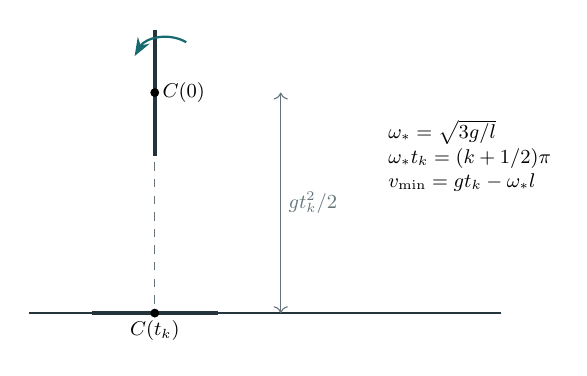
\begin{tikzpicture}[scale=.8,transform shape]

\draw[object] (-2,-3.5)--(5.5,-3.5);
\draw[guide] (0,1)--(0,-3.5);
\draw[object,line width=1.4pt] (0,1)--(0,-1);
\fill (0,0) circle (2pt) node[right] {$C(0)$};
\draw[object,line width=1.4pt] (-1,-3.5)--(1,-3.5);
\fill (0,-3.5) circle (2pt) node[below] {$C(t_k)$};
\draw[axis,<->] (2,0)--(2,-3.5) node[midway,right] {$gt_k^2/2$};
\draw[motion] (.5,.8) arc[start angle=60,end angle=150,radius=.6];
\node[align=left] at (5,-1) {$\omega_*=\sqrt{3g/l}$\\$\omega_*t_k=(k+1/2)\pi$\\$v_{\min}=gt_k-\omega_*l$};

\end{tikzpicture}
\figcaption{解图综四.3C\quad 自由落体质心与匀速转动叠加；各点向下速度和此前最低高度共同确定可行的水平时刻。}
\end{minipage}\end{center}
解图综四.3C以脱梁为$t=0$，用$z_C$表示质心距地高度。此时
\[
z_C=h-l-\frac12gt^2.
\]
以脱梁时指向上端的杆内坐标记作$\zeta$，$-l\leqslant\zeta\leqslant l$，任一点的高度为$z_\zeta=z_C+\zeta\cos(\omega_*t)$。要让一整段杆在同一时刻都位于地面，系数$\cos(\omega_*t)$为零，同时$z_C=0$。这就是杆水平且质心到地面的两个条件，因而候选时刻满足
\[
s_k=\omega_*t_k=\left(k+\frac12\right)\pi,\quad k=0,1,2,\ldots,
\]
\[
h=l+\frac12gt_k^2
=\left[1+\frac{\pi^2}{6}\left(k+\frac12\right)^2\right]l.
\]
水平条件给出几何候选；再以各点向下速度与此前端点高度选择首次整体接触的时刻。由任意点高度求导，向下速度为$gt+\zeta\omega_*\sin(\omega_*t)$。水平时刻正弦的绝对值为1，在整个杆内取最小值，对应旋转速度指向上的那个端点。因此到$t_k$，所有点竖直速度的最小值为
\[
v_{\min}=gt_k-\omega_*l
=\sqrt{\frac{gl}{3}}(s_k-3).
\]
$k=0$时$s_0=\pi/2<3$，有一端在这个水平时刻向上；这一候选轨迹已经与此前的地面接触发生冲突。其高度$h_0=(1+\pi^2/24)l<2l$还使杆在竖直脱梁时的下端低于地面，说明受约束摆下阶段已会先触地。因此取首次整体向下落地时排除$k=0$。$k\ge1$时所有点向下。
\begin{center}\begin{minipage}{.98\linewidth}\centering
\begin{tikzpicture}[scale=.85,transform shape]

\draw[axis] (0,0)--(6.4,0) node[right] {$s=\omega_*t$};
\draw[axis] (0,0)--(0,4.4) node[above] {$d/l$};
\draw[traj,domain=0:4.712389,samples=220] plot ({1.2*\x},{((4.712389^2-\x^2)/6-abs(cos(deg(\x))))});
\draw[guide] (3.7699,0)--(3.7699,3.3);
\node[below] at (3.7699,0) {$s_1-\pi/2$};
\node[below right] at (5.65487,0) {$s_1$};
\node at (3.5,4.5) {$k=1:\ d>0\ (0\le s<s_1)$};
\node at (2.8,-1.2) {早段质心离地大于$l$；末段用$\sin q\le q$};

\end{tikzpicture}
\figcaption{解图综四.3D\quad 最低端高度包络检查整个飞行，在最后水平时刻才首次为零。}
\end{minipage}\end{center}
解图综四.3D以最低端高度覆盖整个下落过程。记$s=\omega_*t$，则最低端距地
\[
\frac{d(s)}l
=\frac{s_k^2-s^2}{6}-|\cos s|,\qquad 0\le s\le s_k.
\]
在任意角位置，杆的两个端点相对质心的高度为$\pm l\cos s$，其中较低者比质心低$l|\cos s|$；所以这个包络同时包含两端，并在穿过水平时自动交换最低端。对$k\ge1$，若$0\le s\le s_k-\pi/2$，有
\[
\frac{s_k^2-s^2}{6}
\ge\frac{\pi s_k-\pi^2/4}{6}
\ge\frac{5\pi^2}{24}>1,
\]
而$|\cos s|\le1$，故$d>0$。最后四分之一转内，令$q=s_k-s\in(0,\pi/2]$，则$|\cos s|=\sin q$，
\[
\frac dl=\frac{q(2s_k-q)}6-\sin q
\ge\frac{5\pi}{12}q-\sin q
\ge\left(\frac{5\pi}{12}-1\right)q>0.
\]
直到$q=0$才有$d=0$，证明更早没有杆端碰地。

上面最后四分之一转的正高度，还可从时间反演读出一个直接的速度意义。令反演时间为$\tau$，从水平着地状态反向上抛质心，其初速为$gt_k$，杆以同样大小的角速度反转。该段里最慢端点的向上速度为
\[
v_{\rm up,min}(\tau)=gt_k-g\tau-\omega_*l\cos(\omega_*\tau),
\qquad0\leqslant\tau\leqslant\frac{\pi}{2\omega_*}.
\]
用单位$\sqrt{gl/3}$表示，需从$s_k$中减去的量为$\omega_*\tau+3\cos(\omega_*\tau)$。在这段中它至多为$\pi/2+3$，而$k\geqslant1$时$s_k\geqslant3\pi/2>\pi/2+3$。故反演的最慢端点仍向上，正演中这最后一段在最终水平之前保持正高度。解图综四.3E画出$k=1$的实际向上速度和上述正下界。
\begin{center}\begin{minipage}{.98\linewidth}\centering
\begin{tikzpicture}[scale=0.72,transform shape]
\draw[axis] (0,0)--(6.2,0);\draw[axis] (0,0)--(0,3.4000000000000004);
\draw[thin,color=muted] (0.0000000,0)--(0.0000000,-.07);\node[below] at (0.0000000,-.09) {$0$};
\draw[thin,color=muted] (3.0000000,0)--(3.0000000,-.07);\node[below] at (3.0000000,-.09) {$\pi/4$};
\draw[thin,color=muted] (6.0000000,0)--(6.0000000,-.07);\node[below] at (6.0000000,-.09) {$\pi/2$};
\draw[thin,color=muted] (0,0.0000000)--(-.07,0.0000000);\node[left] at (-.09,0.0000000) {$0$};
\draw[thin,color=muted] (0,0.9696970)--(-.07,0.9696970);\node[left] at (-.09,0.9696970) {$1$};
\draw[thin,color=muted] (0,1.9393939)--(-.07,1.9393939);\node[left] at (-.09,1.9393939) {$2$};
\draw[thin,color=muted] (0,2.9090909)--(-.07,2.9090909);\node[left] at (-.09,2.9090909) {$3$};
\node[below] at (3.0,-.64) {反演角时间$q=\omega_*\tau$};\node[above right] at (0,3.45) {速度除以$\sqrt{gl/3}$};
\draw[traj] plot coordinates {(0.0000000,1.6604984) (0.0200000,1.6554610) (0.0400000,1.6505033) (0.0600000,1.6456253) (0.0800000,1.6408271) (0.1000000,1.6361087) (0.1200000,1.6314699) (0.1400000,1.6269109) (0.1600000,1.6224316) (0.1800000,1.6180320) (0.2000000,1.6137120) (0.2200000,1.6094717) (0.2400000,1.6053110) (0.2600000,1.6012299) (0.2800000,1.5972283) (0.3000000,1.5933063) (0.3200000,1.5894639) (0.3400000,1.5857008) (0.3600000,1.5820173) (0.3800000,1.5784131) (0.4000000,1.5748883) (0.4200000,1.5714428) (0.4400000,1.5680766) (0.4600000,1.5647896) (0.4800000,1.5615817) (0.5000000,1.5584530) (0.5200000,1.5554034) (0.5400000,1.5524328) (0.5600000,1.5495412) (0.5800000,1.5467284) (0.6000000,1.5439945) (0.6200000,1.5413394) (0.6400000,1.5387629) (0.6600000,1.5362651) (0.6800000,1.5338459) (0.7000000,1.5315052) (0.7200000,1.5292428) (0.7400000,1.5270589) (0.7600000,1.5249531) (0.7800000,1.5229256) (0.8000000,1.5209762) (0.8200000,1.5191047) (0.8400000,1.5173112) (0.8600000,1.5155956) (0.8800000,1.5139576) (0.9000000,1.5123974) (0.9200000,1.5109146) (0.9400000,1.5095093) (0.9600000,1.5081814) (0.9800000,1.5069307) (1.0000000,1.5057572) (1.0200000,1.5046607) (1.0400000,1.5036411) (1.0600000,1.5026984) (1.0800000,1.5018323) (1.1000000,1.5010429) (1.1200000,1.5003299) (1.1400000,1.4996932) (1.1600000,1.4991328) (1.1800000,1.4986485) (1.2000000,1.4982402) (1.2200000,1.4979077) (1.2400000,1.4976509) (1.2600000,1.4974697) (1.2800000,1.4973640) (1.3000000,1.4973336) (1.3200000,1.4973784) (1.3400000,1.4974982) (1.3600000,1.4976929) (1.3800000,1.4979624) (1.4000000,1.4983065) (1.4200000,1.4987250) (1.4400000,1.4992178) (1.4600000,1.4997848) (1.4800000,1.5004258) (1.5000000,1.5011407) (1.5200000,1.5019292) (1.5400000,1.5027912) (1.5600000,1.5037266) (1.5800000,1.5047352) (1.6000000,1.5058168) (1.6200000,1.5069713) (1.6400000,1.5081985) (1.6600000,1.5094981) (1.6800000,1.5108702) (1.7000000,1.5123143) (1.7200000,1.5138305) (1.7400000,1.5154185) (1.7600000,1.5170781) (1.7800000,1.5188091) (1.8000000,1.5206114) (1.8200000,1.5224847) (1.8400000,1.5244290) (1.8600000,1.5264439) (1.8800000,1.5285292) (1.9000000,1.5306849) (1.9200000,1.5329107) (1.9400000,1.5352063) (1.9600000,1.5375716) (1.9800000,1.5400064) (2.0000000,1.5425105) (2.0200000,1.5450837) (2.0400000,1.5477257) (2.0600000,1.5504364) (2.0800000,1.5532155) (2.1000000,1.5560628) (2.1200000,1.5589781) (2.1400000,1.5619612) (2.1600000,1.5650119) (2.1800000,1.5681299) (2.2000000,1.5713150) (2.2200000,1.5745670) (2.2400000,1.5778857) (2.2600000,1.5812708) (2.2800000,1.5847221) (2.3000000,1.5882393) (2.3200000,1.5918223) (2.3400000,1.5954708) (2.3600000,1.5991845) (2.3800000,1.6029633) (2.4000000,1.6068068) (2.4200000,1.6107148) (2.4400000,1.6146871) (2.4600000,1.6187234) (2.4800000,1.6228235) (2.5000000,1.6269871) (2.5200000,1.6312140) (2.5400000,1.6355040) (2.5600000,1.6398567) (2.5800000,1.6442718) (2.6000000,1.6487493) (2.6200000,1.6532887) (2.6400000,1.6578898) (2.6600000,1.6625524) (2.6800000,1.6672762) (2.7000000,1.6720608) (2.7200000,1.6769062) (2.7400000,1.6818119) (2.7600000,1.6867777) (2.7800000,1.6918033) (2.8000000,1.6968885) (2.8200000,1.7020329) (2.8400000,1.7072363) (2.8600000,1.7124985) (2.8800000,1.7178190) (2.9000000,1.7231977) (2.9200000,1.7286343) (2.9400000,1.7341284) (2.9600000,1.7396798) (2.9800000,1.7452881) (3.0000000,1.7509532) (3.0200000,1.7566746) (3.0400000,1.7624522) (3.0600000,1.7682855) (3.0800000,1.7741744) (3.1000000,1.7801184) (3.1200000,1.7861174) (3.1400000,1.7921710) (3.1600000,1.7982788) (3.1800000,1.8044406) (3.2000000,1.8106561) (3.2200000,1.8169250) (3.2400000,1.8232469) (3.2600000,1.8296216) (3.2800000,1.8360487) (3.3000000,1.8425279) (3.3200000,1.8490589) (3.3400000,1.8556413) (3.3600000,1.8622750) (3.3800000,1.8689594) (3.4000000,1.8756944) (3.4200000,1.8824796) (3.4400000,1.8893147) (3.4600000,1.8961992) (3.4800000,1.9031330) (3.5000000,1.9101157) (3.5200000,1.9171469) (3.5400000,1.9242264) (3.5600000,1.9313537) (3.5800000,1.9385286) (3.6000000,1.9457507) (3.6200000,1.9530197) (3.6400000,1.9603352) (3.6600000,1.9676969) (3.6800000,1.9751045) (3.7000000,1.9825576) (3.7200000,1.9900559) (3.7400000,1.9975990) (3.7600000,2.0051866) (3.7800000,2.0128183) (3.8000000,2.0204938) (3.8200000,2.0282127) (3.8400000,2.0359747) (3.8600000,2.0437795) (3.8800000,2.0516266) (3.9000000,2.0595158) (3.9200000,2.0674466) (3.9400000,2.0754188) (3.9600000,2.0834319) (3.9800000,2.0914856) (4.0000000,2.0995796) (4.0200000,2.1077134) (4.0400000,2.1158867) (4.0600000,2.1240992) (4.0800000,2.1323505) (4.1000000,2.1406402) (4.1200000,2.1489680) (4.1400000,2.1573334) (4.1600000,2.1657362) (4.1800000,2.1741759) (4.2000000,2.1826522) (4.2200000,2.1911647) (4.2400000,2.1997130) (4.2600000,2.2082968) (4.2800000,2.2169157) (4.3000000,2.2255693) (4.3200000,2.2342572) (4.3400000,2.2429791) (4.3600000,2.2517346) (4.3800000,2.2605232) (4.4000000,2.2693447) (4.4200000,2.2781986) (4.4400000,2.2870846) (4.4600000,2.2960023) (4.4800000,2.3049512) (4.5000000,2.3139311) (4.5200000,2.3229415) (4.5400000,2.3319820) (4.5600000,2.3410522) (4.5800000,2.3501518) (4.6000000,2.3592804) (4.6200000,2.3684376) (4.6400000,2.3776230) (4.6600000,2.3868361) (4.6800000,2.3960767) (4.7000000,2.4053443) (4.7200000,2.4146385) (4.7400000,2.4239589) (4.7600000,2.4333052) (4.7800000,2.4426769) (4.8000000,2.4520736) (4.8200000,2.4614950) (4.8400000,2.4709407) (4.8600000,2.4804102) (4.8800000,2.4899031) (4.9000000,2.4994191) (4.9200000,2.5089577) (4.9400000,2.5185186) (4.9600000,2.5281014) (4.9800000,2.5377056) (5.0000000,2.5473308) (5.0200000,2.5569767) (5.0400000,2.5666428) (5.0600000,2.5763288) (5.0800000,2.5860342) (5.1000000,2.5957586) (5.1200000,2.6055016) (5.1400000,2.6152628) (5.1600000,2.6250419) (5.1800000,2.6348383) (5.2000000,2.6446517) (5.2200000,2.6544817) (5.2400000,2.6643279) (5.2600000,2.6741899) (5.2800000,2.6840672) (5.3000000,2.6939594) (5.3200000,2.7038662) (5.3400000,2.7137871) (5.3600000,2.7237217) (5.3800000,2.7336696) (5.4000000,2.7436304) (5.4200000,2.7536037) (5.4400000,2.7635891) (5.4600000,2.7735861) (5.4800000,2.7835943) (5.5000000,2.7936134) (5.5200000,2.8036428) (5.5400000,2.8136823) (5.5600000,2.8237313) (5.5800000,2.8337895) (5.6000000,2.8438565) (5.6200000,2.8539318) (5.6400000,2.8640150) (5.6600000,2.8741058) (5.6800000,2.8842036) (5.7000000,2.8943081) (5.7200000,2.9044188) (5.7400000,2.9145354) (5.7600000,2.9246574) (5.7800000,2.9347844) (5.8000000,2.9449160) (5.8200000,2.9550518) (5.8400000,2.9651914) (5.8600000,2.9753342) (5.8800000,2.9854801) (5.9000000,2.9956284) (5.9200000,3.0057788) (5.9400000,3.0159308) (5.9600000,3.0260841) (5.9800000,3.0362383) (6.0000000,3.0463929)};
\draw[traj] (.1,-1.05)--(.7,-1.05);\node[right] at (.85,-1.05) {最慢端点实际向上速度};\draw[dashed,thick,color=warm] plot coordinates {(0.0000000,0.1373020) (0.0200000,0.1373020) (0.0400000,0.1373020) (0.0600000,0.1373020) (0.0800000,0.1373020) (0.1000000,0.1373020) (0.1200000,0.1373020) (0.1400000,0.1373020) (0.1600000,0.1373020) (0.1800000,0.1373020) (0.2000000,0.1373020) (0.2200000,0.1373020) (0.2400000,0.1373020) (0.2600000,0.1373020) (0.2800000,0.1373020) (0.3000000,0.1373020) (0.3200000,0.1373020) (0.3400000,0.1373020) (0.3600000,0.1373020) (0.3800000,0.1373020) (0.4000000,0.1373020) (0.4200000,0.1373020) (0.4400000,0.1373020) (0.4600000,0.1373020) (0.4800000,0.1373020) (0.5000000,0.1373020) (0.5200000,0.1373020) (0.5400000,0.1373020) (0.5600000,0.1373020) (0.5800000,0.1373020) (0.6000000,0.1373020) (0.6200000,0.1373020) (0.6400000,0.1373020) (0.6600000,0.1373020) (0.6800000,0.1373020) (0.7000000,0.1373020) (0.7200000,0.1373020) (0.7400000,0.1373020) (0.7600000,0.1373020) (0.7800000,0.1373020) (0.8000000,0.1373020) (0.8200000,0.1373020) (0.8400000,0.1373020) (0.8600000,0.1373020) (0.8800000,0.1373020) (0.9000000,0.1373020) (0.9200000,0.1373020) (0.9400000,0.1373020) (0.9600000,0.1373020) (0.9800000,0.1373020) (1.0000000,0.1373020) (1.0200000,0.1373020) (1.0400000,0.1373020) (1.0600000,0.1373020) (1.0800000,0.1373020) (1.1000000,0.1373020) (1.1200000,0.1373020) (1.1400000,0.1373020) (1.1600000,0.1373020) (1.1800000,0.1373020) (1.2000000,0.1373020) (1.2200000,0.1373020) (1.2400000,0.1373020) (1.2600000,0.1373020) (1.2800000,0.1373020) (1.3000000,0.1373020) (1.3200000,0.1373020) (1.3400000,0.1373020) (1.3600000,0.1373020) (1.3800000,0.1373020) (1.4000000,0.1373020) (1.4200000,0.1373020) (1.4400000,0.1373020) (1.4600000,0.1373020) (1.4800000,0.1373020) (1.5000000,0.1373020) (1.5200000,0.1373020) (1.5400000,0.1373020) (1.5600000,0.1373020) (1.5800000,0.1373020) (1.6000000,0.1373020) (1.6200000,0.1373020) (1.6400000,0.1373020) (1.6600000,0.1373020) (1.6800000,0.1373020) (1.7000000,0.1373020) (1.7200000,0.1373020) (1.7400000,0.1373020) (1.7600000,0.1373020) (1.7800000,0.1373020) (1.8000000,0.1373020) (1.8200000,0.1373020) (1.8400000,0.1373020) (1.8600000,0.1373020) (1.8800000,0.1373020) (1.9000000,0.1373020) (1.9200000,0.1373020) (1.9400000,0.1373020) (1.9600000,0.1373020) (1.9800000,0.1373020) (2.0000000,0.1373020) (2.0200000,0.1373020) (2.0400000,0.1373020) (2.0600000,0.1373020) (2.0800000,0.1373020) (2.1000000,0.1373020) (2.1200000,0.1373020) (2.1400000,0.1373020) (2.1600000,0.1373020) (2.1800000,0.1373020) (2.2000000,0.1373020) (2.2200000,0.1373020) (2.2400000,0.1373020) (2.2600000,0.1373020) (2.2800000,0.1373020) (2.3000000,0.1373020) (2.3200000,0.1373020) (2.3400000,0.1373020) (2.3600000,0.1373020) (2.3800000,0.1373020) (2.4000000,0.1373020) (2.4200000,0.1373020) (2.4400000,0.1373020) (2.4600000,0.1373020) (2.4800000,0.1373020) (2.5000000,0.1373020) (2.5200000,0.1373020) (2.5400000,0.1373020) (2.5600000,0.1373020) (2.5800000,0.1373020) (2.6000000,0.1373020) (2.6200000,0.1373020) (2.6400000,0.1373020) (2.6600000,0.1373020) (2.6800000,0.1373020) (2.7000000,0.1373020) (2.7200000,0.1373020) (2.7400000,0.1373020) (2.7600000,0.1373020) (2.7800000,0.1373020) (2.8000000,0.1373020) (2.8200000,0.1373020) (2.8400000,0.1373020) (2.8600000,0.1373020) (2.8800000,0.1373020) (2.9000000,0.1373020) (2.9200000,0.1373020) (2.9400000,0.1373020) (2.9600000,0.1373020) (2.9800000,0.1373020) (3.0000000,0.1373020) (3.0200000,0.1373020) (3.0400000,0.1373020) (3.0600000,0.1373020) (3.0800000,0.1373020) (3.1000000,0.1373020) (3.1200000,0.1373020) (3.1400000,0.1373020) (3.1600000,0.1373020) (3.1800000,0.1373020) (3.2000000,0.1373020) (3.2200000,0.1373020) (3.2400000,0.1373020) (3.2600000,0.1373020) (3.2800000,0.1373020) (3.3000000,0.1373020) (3.3200000,0.1373020) (3.3400000,0.1373020) (3.3600000,0.1373020) (3.3800000,0.1373020) (3.4000000,0.1373020) (3.4200000,0.1373020) (3.4400000,0.1373020) (3.4600000,0.1373020) (3.4800000,0.1373020) (3.5000000,0.1373020) (3.5200000,0.1373020) (3.5400000,0.1373020) (3.5600000,0.1373020) (3.5800000,0.1373020) (3.6000000,0.1373020) (3.6200000,0.1373020) (3.6400000,0.1373020) (3.6600000,0.1373020) (3.6800000,0.1373020) (3.7000000,0.1373020) (3.7200000,0.1373020) (3.7400000,0.1373020) (3.7600000,0.1373020) (3.7800000,0.1373020) (3.8000000,0.1373020) (3.8200000,0.1373020) (3.8400000,0.1373020) (3.8600000,0.1373020) (3.8800000,0.1373020) (3.9000000,0.1373020) (3.9200000,0.1373020) (3.9400000,0.1373020) (3.9600000,0.1373020) (3.9800000,0.1373020) (4.0000000,0.1373020) (4.0200000,0.1373020) (4.0400000,0.1373020) (4.0600000,0.1373020) (4.0800000,0.1373020) (4.1000000,0.1373020) (4.1200000,0.1373020) (4.1400000,0.1373020) (4.1600000,0.1373020) (4.1800000,0.1373020) (4.2000000,0.1373020) (4.2200000,0.1373020) (4.2400000,0.1373020) (4.2600000,0.1373020) (4.2800000,0.1373020) (4.3000000,0.1373020) (4.3200000,0.1373020) (4.3400000,0.1373020) (4.3600000,0.1373020) (4.3800000,0.1373020) (4.4000000,0.1373020) (4.4200000,0.1373020) (4.4400000,0.1373020) (4.4600000,0.1373020) (4.4800000,0.1373020) (4.5000000,0.1373020) (4.5200000,0.1373020) (4.5400000,0.1373020) (4.5600000,0.1373020) (4.5800000,0.1373020) (4.6000000,0.1373020) (4.6200000,0.1373020) (4.6400000,0.1373020) (4.6600000,0.1373020) (4.6800000,0.1373020) (4.7000000,0.1373020) (4.7200000,0.1373020) (4.7400000,0.1373020) (4.7600000,0.1373020) (4.7800000,0.1373020) (4.8000000,0.1373020) (4.8200000,0.1373020) (4.8400000,0.1373020) (4.8600000,0.1373020) (4.8800000,0.1373020) (4.9000000,0.1373020) (4.9200000,0.1373020) (4.9400000,0.1373020) (4.9600000,0.1373020) (4.9800000,0.1373020) (5.0000000,0.1373020) (5.0200000,0.1373020) (5.0400000,0.1373020) (5.0600000,0.1373020) (5.0800000,0.1373020) (5.1000000,0.1373020) (5.1200000,0.1373020) (5.1400000,0.1373020) (5.1600000,0.1373020) (5.1800000,0.1373020) (5.2000000,0.1373020) (5.2200000,0.1373020) (5.2400000,0.1373020) (5.2600000,0.1373020) (5.2800000,0.1373020) (5.3000000,0.1373020) (5.3200000,0.1373020) (5.3400000,0.1373020) (5.3600000,0.1373020) (5.3800000,0.1373020) (5.4000000,0.1373020) (5.4200000,0.1373020) (5.4400000,0.1373020) (5.4600000,0.1373020) (5.4800000,0.1373020) (5.5000000,0.1373020) (5.5200000,0.1373020) (5.5400000,0.1373020) (5.5600000,0.1373020) (5.5800000,0.1373020) (5.6000000,0.1373020) (5.6200000,0.1373020) (5.6400000,0.1373020) (5.6600000,0.1373020) (5.6800000,0.1373020) (5.7000000,0.1373020) (5.7200000,0.1373020) (5.7400000,0.1373020) (5.7600000,0.1373020) (5.7800000,0.1373020) (5.8000000,0.1373020) (5.8200000,0.1373020) (5.8400000,0.1373020) (5.8600000,0.1373020) (5.8800000,0.1373020) (5.9000000,0.1373020) (5.9200000,0.1373020) (5.9400000,0.1373020) (5.9600000,0.1373020) (5.9800000,0.1373020) (6.0000000,0.1373020)};
\draw[dashed,thick,color=warm] (.1,-1.48)--(.7,-1.48);\node[right] at (.85,-1.48) {统一正下界};\end{tikzpicture}
\figcaption{解图综四.3E\quad k等于1时反演的最慢端点仍上升，正演末段在最终水平前保持分离}
\end{minipage}\end{center}
最终允许的横梁高度是
\[
\boxed{h=\left[1+\frac{\pi^2}{6}\left(k+\frac12\right)^2\right]l,\qquad k=1,2,\ldots}.
\]
最小值为$h_{\min}=(1+3\pi^2/8)l\simeq4.70l$。这个高度也大于$2l$，因此脱梁前的整个摆下阶段，杆的下端高度$h-2l\cos\phi\geqslant h-2l>0$，与地面保持分离。允许高度的离散性由匀速转动的水平时刻与质心的二次下落位移共同确定；质量在重力势能和惯量中同时约去，所以高度比$h/l$与杆质量无关。完整条件由水平几何、全杆向下速度和全程正高度共同组成，因而选出$k=1,2,\ldots$这一离散高度族。


\Needspace{8\baselineskip}

\pdfbookmark[3]{关键洞察}{q3-h5}

\subsection*{关键洞察}

杆的端点在滑动，动能使用质心分解自然满足实际约束。速度比较依赖同一角区间内的点态排序，若函数交叉便比较完整时间积分。杆水平与全杆同时向下首次触地是三条不同条件的结合；最早水平候选既有向上端点，又与脱梁前竖直长度冲突。全程证明先以质心高度控制早段，末段再用正弦上界或反演速度。

\Needspace{8\baselineskip}

\pdfbookmark[3]{易错点}{q3-h6}

\subsection*{易错点}

60度幅角保留完整三角函数，周期由有限幅运动决定。滑动端的速度进入约束，固定轴动能式应按实际端点状态使用。竖直时质心速度为零、角速度最大，释放后保留这组初值。最低端在水平穿越时交换，包络用$|\cos s|$同时跟踪两端；地面分离覆盖释放前和释放后的全部时间。

\Needspace{8\baselineskip}

\pdfbookmark[3]{课堂讲解建议}{q3-h7}

\subsection*{课堂讲解建议}

在两个偏角处标出$A,C$，先问哪个水平坐标不动，学生回答质心$C$，再由几何关系求滑动端左移量。比较周期时将直观猜测转为全区间速度比，并解释转折点的可积时间微元。画$k=0$水平候选的两端速度，指出其中一端仍向上，随后比较它的梁高与$2l$，说明此前已经发生地面接触。最后分早段与末四分之一转建立正高度证据，反演图E补充末段的速度解释。

\Needspace{8\baselineskip}

\pdfbookmark[3]{变式训练}{q3-h8}

\subsection*{变式训练}

\begin{enumerate}
\Needspace{37\baselineskip}
\item \textbf{题设与求解。} 单摆长改为$L$、共同振幅为$\alpha$，给出直接比较周期的充分条件。角速度平方比仍为$3L/[l(1+3\sin^2\phi)]$。令$M_\alpha=\max_{|\phi|\leqslant\alpha}\sin^2\phi$，则$\alpha\leqslant\pi/2$时$M_\alpha=\sin^2\alpha$，$\pi/2<\alpha<\pi$时$M_\alpha=1$。若$3L/l>1+3M_\alpha$，杆全程角速度更大，周期更短；若$3L/l<1$，杆更慢、周期更长。中间参数的速度函数可交叉，采用时间积分作整体比较。图V1取60度振幅，画同角速度平方比及不同摆长对应的位置。
\begin{center}\begin{minipage}{.98\linewidth}\centering
\begin{tikzpicture}[scale=0.72,transform shape]
\draw[axis] (0,0)--(6.2,0);\draw[axis] (0,0)--(0,3.4000000000000004);
\draw[thin,color=muted] (0.0000000,0)--(0.0000000,-.07);\node[below] at (0.0000000,-.09) {$-60$};
\draw[thin,color=muted] (3.0000000,0)--(3.0000000,-.07);\node[below] at (3.0000000,-.09) {$0$};
\draw[thin,color=muted] (6.0000000,0)--(6.0000000,-.07);\node[below] at (6.0000000,-.09) {$60$};
\draw[thin,color=muted] (0,0.0000000)--(-.07,0.0000000);\node[left] at (-.09,0.0000000) {$0$};
\draw[thin,color=muted] (0,0.9142857)--(-.07,0.9142857);\node[left] at (-.09,0.9142857) {$1$};
\draw[thin,color=muted] (0,1.8285714)--(-.07,1.8285714);\node[left] at (-.09,1.8285714) {$2$};
\draw[thin,color=muted] (0,2.7428571)--(-.07,2.7428571);\node[left] at (-.09,2.7428571) {$3$};
\node[below] at (3.0,-.64) {共同偏角$\phi$（度）};\node[above right] at (0,3.45) {$\omega_{\rm rod}^2/\omega_{\rm pend}^2$};
\draw[traj] plot coordinates {(0.0000000,0.2531868) (0.0250000,0.2549744) (0.0500000,0.2568052) (0.0750000,0.2586799) (0.1000000,0.2605993) (0.1250000,0.2625642) (0.1500000,0.2645754) (0.1750000,0.2666336) (0.2000000,0.2687398) (0.2250000,0.2708948) (0.2500000,0.2730995) (0.2750000,0.2753548) (0.3000000,0.2776616) (0.3250000,0.2800208) (0.3500000,0.2824333) (0.3750000,0.2849003) (0.4000000,0.2874226) (0.4250000,0.2900012) (0.4500000,0.2926372) (0.4750000,0.2953317) (0.5000000,0.2980856) (0.5250000,0.3009002) (0.5500000,0.3037764) (0.5750000,0.3067153) (0.6000000,0.3097182) (0.6250000,0.3127862) (0.6500000,0.3159204) (0.6750000,0.3191219) (0.7000000,0.3223921) (0.7250000,0.3257320) (0.7500000,0.3291429) (0.7750000,0.3326259) (0.8000000,0.3361824) (0.8250000,0.3398135) (0.8500000,0.3435205) (0.8750000,0.3473046) (0.9000000,0.3511670) (0.9250000,0.3551090) (0.9500000,0.3591317) (0.9750000,0.3632365) (1.0000000,0.3674244) (1.0250000,0.3716967) (1.0500000,0.3760545) (1.0750000,0.3804991) (1.1000000,0.3850314) (1.1250000,0.3896526) (1.1500000,0.3943637) (1.1750000,0.3991657) (1.2000000,0.4040596) (1.2250000,0.4090463) (1.2500000,0.4141267) (1.2750000,0.4193014) (1.3000000,0.4245711) (1.3250000,0.4299366) (1.3500000,0.4353983) (1.3750000,0.4409567) (1.4000000,0.4466119) (1.4250000,0.4523643) (1.4500000,0.4582139) (1.4750000,0.4641606) (1.5000000,0.4702041) (1.5250000,0.4763441) (1.5500000,0.4825799) (1.5750000,0.4889108) (1.6000000,0.4953358) (1.6250000,0.5018537) (1.6500000,0.5084631) (1.6750000,0.5151623) (1.7000000,0.5219493) (1.7250000,0.5288219) (1.7500000,0.5357776) (1.7750000,0.5428135) (1.8000000,0.5499264) (1.8250000,0.5571129) (1.8500000,0.5643691) (1.8750000,0.5716907) (1.9000000,0.5790730) (1.9250000,0.5865111) (1.9500000,0.5939994) (1.9750000,0.6015321) (2.0000000,0.6091027) (2.0250000,0.6167045) (2.0500000,0.6243302) (2.0750000,0.6319720) (2.1000000,0.6396218) (2.1250000,0.6472708) (2.1500000,0.6549097) (2.1750000,0.6625290) (2.2000000,0.6701185) (2.2250000,0.6776675) (2.2500000,0.6851651) (2.2750000,0.6925996) (2.3000000,0.6999593) (2.3250000,0.7072317) (2.3500000,0.7144042) (2.3750000,0.7214638) (2.4000000,0.7283973) (2.4250000,0.7351910) (2.4500000,0.7418312) (2.4750000,0.7483041) (2.5000000,0.7545956) (2.5250000,0.7606918) (2.5500000,0.7665786) (2.5750000,0.7722422) (2.6000000,0.7776688) (2.6250000,0.7828450) (2.6500000,0.7877575) (2.6750000,0.7923936) (2.7000000,0.7967411) (2.7250000,0.8007880) (2.7500000,0.8045234) (2.7750000,0.8079366) (2.8000000,0.8110180) (2.8250000,0.8137587) (2.8500000,0.8161507) (2.8750000,0.8181870) (2.9000000,0.8198614) (2.9250000,0.8211691) (2.9500000,0.8221059) (2.9750000,0.8226692) (3.0000000,0.8228571) (3.0250000,0.8226692) (3.0500000,0.8221059) (3.0750000,0.8211691) (3.1000000,0.8198614) (3.1250000,0.8181870) (3.1500000,0.8161507) (3.1750000,0.8137587) (3.2000000,0.8110180) (3.2250000,0.8079366) (3.2500000,0.8045234) (3.2750000,0.8007880) (3.3000000,0.7967411) (3.3250000,0.7923936) (3.3500000,0.7877575) (3.3750000,0.7828450) (3.4000000,0.7776688) (3.4250000,0.7722422) (3.4500000,0.7665786) (3.4750000,0.7606918) (3.5000000,0.7545956) (3.5250000,0.7483041) (3.5500000,0.7418312) (3.5750000,0.7351910) (3.6000000,0.7283973) (3.6250000,0.7214638) (3.6500000,0.7144042) (3.6750000,0.7072317) (3.7000000,0.6999593) (3.7250000,0.6925996) (3.7500000,0.6851651) (3.7750000,0.6776675) (3.8000000,0.6701185) (3.8250000,0.6625290) (3.8500000,0.6549097) (3.8750000,0.6472708) (3.9000000,0.6396218) (3.9250000,0.6319720) (3.9500000,0.6243302) (3.9750000,0.6167045) (4.0000000,0.6091027) (4.0250000,0.6015321) (4.0500000,0.5939994) (4.0750000,0.5865111) (4.1000000,0.5790730) (4.1250000,0.5716907) (4.1500000,0.5643691) (4.1750000,0.5571129) (4.2000000,0.5499264) (4.2250000,0.5428135) (4.2500000,0.5357776) (4.2750000,0.5288219) (4.3000000,0.5219493) (4.3250000,0.5151623) (4.3500000,0.5084631) (4.3750000,0.5018537) (4.4000000,0.4953358) (4.4250000,0.4889108) (4.4500000,0.4825799) (4.4750000,0.4763441) (4.5000000,0.4702041) (4.5250000,0.4641606) (4.5500000,0.4582139) (4.5750000,0.4523643) (4.6000000,0.4466119) (4.6250000,0.4409567) (4.6500000,0.4353983) (4.6750000,0.4299366) (4.7000000,0.4245711) (4.7250000,0.4193014) (4.7500000,0.4141267) (4.7750000,0.4090463) (4.8000000,0.4040596) (4.8250000,0.3991657) (4.8500000,0.3943637) (4.8750000,0.3896526) (4.9000000,0.3850314) (4.9250000,0.3804991) (4.9500000,0.3760545) (4.9750000,0.3716967) (5.0000000,0.3674244) (5.0250000,0.3632365) (5.0500000,0.3591317) (5.0750000,0.3551090) (5.1000000,0.3511670) (5.1250000,0.3473046) (5.1500000,0.3435205) (5.1750000,0.3398135) (5.2000000,0.3361824) (5.2250000,0.3326259) (5.2500000,0.3291429) (5.2750000,0.3257320) (5.3000000,0.3223921) (5.3250000,0.3191219) (5.3500000,0.3159204) (5.3750000,0.3127862) (5.4000000,0.3097182) (5.4250000,0.3067153) (5.4500000,0.3037764) (5.4750000,0.3009002) (5.5000000,0.2980856) (5.5250000,0.2953317) (5.5500000,0.2926372) (5.5750000,0.2900012) (5.6000000,0.2874226) (5.6250000,0.2849003) (5.6500000,0.2824333) (5.6750000,0.2800208) (5.7000000,0.2776616) (5.7250000,0.2753548) (5.7500000,0.2730995) (5.7750000,0.2708948) (5.8000000,0.2687398) (5.8250000,0.2666336) (5.8500000,0.2645754) (5.8750000,0.2625642) (5.9000000,0.2605993) (5.9250000,0.2586799) (5.9500000,0.2568052) (5.9750000,0.2549744) (6.0000000,0.2531868)};
\draw[traj] (.1,-1.05)--(.7,-1.05);\node[right] at (.85,-1.05) {$L/l=.3$};\draw[dashed,thick,color=warm] plot coordinates {(0.0000000,0.8439560) (0.0250000,0.8499147) (0.0500000,0.8560174) (0.0750000,0.8622664) (0.1000000,0.8686644) (0.1250000,0.8752140) (0.1500000,0.8819179) (0.1750000,0.8887787) (0.2000000,0.8957994) (0.2250000,0.9029828) (0.2500000,0.9103318) (0.2750000,0.9178493) (0.3000000,0.9255386) (0.3250000,0.9334026) (0.3500000,0.9414445) (0.3750000,0.9496676) (0.4000000,0.9580752) (0.4250000,0.9666707) (0.4500000,0.9754575) (0.4750000,0.9844390) (0.5000000,0.9936188) (0.5250000,1.0030005) (0.5500000,1.0125879) (0.5750000,1.0223845) (0.6000000,1.0323941) (0.6250000,1.0426206) (0.6500000,1.0530679) (0.6750000,1.0637398) (0.7000000,1.0746402) (0.7250000,1.0857732) (0.7500000,1.0971429) (0.7750000,1.1087531) (0.8000000,1.1206081) (0.8250000,1.1327118) (0.8500000,1.1450684) (0.8750000,1.1576820) (0.9000000,1.1705568) (0.9250000,1.1836967) (0.9500000,1.1971058) (0.9750000,1.2107883) (1.0000000,1.2247480) (1.0250000,1.2389890) (1.0500000,1.2535151) (1.0750000,1.2683302) (1.1000000,1.2834379) (1.1250000,1.2988419) (1.1500000,1.3145456) (1.1750000,1.3305524) (1.2000000,1.3468654) (1.2250000,1.3634878) (1.2500000,1.3804222) (1.2750000,1.3976712) (1.3000000,1.4152372) (1.3250000,1.4331221) (1.3500000,1.4513278) (1.3750000,1.4698555) (1.4000000,1.4887064) (1.4250000,1.5078811) (1.4500000,1.5273796) (1.4750000,1.5472019) (1.5000000,1.5673469) (1.5250000,1.5878135) (1.5500000,1.6085996) (1.5750000,1.6297027) (1.6000000,1.6511194) (1.6250000,1.6728458) (1.6500000,1.6948771) (1.6750000,1.7172077) (1.7000000,1.7398310) (1.7250000,1.7627397) (1.7500000,1.7859252) (1.7750000,1.8093782) (1.8000000,1.8330880) (1.8250000,1.8570430) (1.8500000,1.8812303) (1.8750000,1.9056355) (1.9000000,1.9302434) (1.9250000,1.9550370) (1.9500000,1.9799980) (1.9750000,2.0051069) (2.0000000,2.0303423) (2.0250000,2.0556817) (2.0500000,2.0811007) (2.0750000,2.1065735) (2.1000000,2.1320727) (2.1250000,2.1575692) (2.1500000,2.1830324) (2.1750000,2.2084300) (2.2000000,2.2337283) (2.2250000,2.2588917) (2.2500000,2.2838836) (2.2750000,2.3086654) (2.3000000,2.3331976) (2.3250000,2.3574389) (2.3500000,2.3813473) (2.3750000,2.4048794) (2.4000000,2.4279909) (2.4250000,2.4506366) (2.4500000,2.4727707) (2.4750000,2.4943470) (2.5000000,2.5153187) (2.5250000,2.5356393) (2.5500000,2.5552620) (2.5750000,2.5741406) (2.6000000,2.5922293) (2.6250000,2.6094832) (2.6500000,2.6258583) (2.6750000,2.6413122) (2.7000000,2.6558036) (2.7250000,2.6692935) (2.7500000,2.6817446) (2.7750000,2.6931219) (2.8000000,2.7033933) (2.8250000,2.7125290) (2.8500000,2.7205023) (2.8750000,2.7272899) (2.9000000,2.7328714) (2.9250000,2.7372302) (2.9500000,2.7403531) (2.9750000,2.7422307) (3.0000000,2.7428571) (3.0250000,2.7422307) (3.0500000,2.7403531) (3.0750000,2.7372302) (3.1000000,2.7328714) (3.1250000,2.7272899) (3.1500000,2.7205023) (3.1750000,2.7125290) (3.2000000,2.7033933) (3.2250000,2.6931219) (3.2500000,2.6817446) (3.2750000,2.6692935) (3.3000000,2.6558036) (3.3250000,2.6413122) (3.3500000,2.6258583) (3.3750000,2.6094832) (3.4000000,2.5922293) (3.4250000,2.5741406) (3.4500000,2.5552620) (3.4750000,2.5356393) (3.5000000,2.5153187) (3.5250000,2.4943470) (3.5500000,2.4727707) (3.5750000,2.4506366) (3.6000000,2.4279909) (3.6250000,2.4048794) (3.6500000,2.3813473) (3.6750000,2.3574389) (3.7000000,2.3331976) (3.7250000,2.3086654) (3.7500000,2.2838836) (3.7750000,2.2588917) (3.8000000,2.2337283) (3.8250000,2.2084300) (3.8500000,2.1830324) (3.8750000,2.1575692) (3.9000000,2.1320727) (3.9250000,2.1065735) (3.9500000,2.0811007) (3.9750000,2.0556817) (4.0000000,2.0303423) (4.0250000,2.0051069) (4.0500000,1.9799980) (4.0750000,1.9550370) (4.1000000,1.9302434) (4.1250000,1.9056355) (4.1500000,1.8812303) (4.1750000,1.8570430) (4.2000000,1.8330880) (4.2250000,1.8093782) (4.2500000,1.7859252) (4.2750000,1.7627397) (4.3000000,1.7398310) (4.3250000,1.7172077) (4.3500000,1.6948771) (4.3750000,1.6728458) (4.4000000,1.6511194) (4.4250000,1.6297027) (4.4500000,1.6085996) (4.4750000,1.5878135) (4.5000000,1.5673469) (4.5250000,1.5472019) (4.5500000,1.5273796) (4.5750000,1.5078811) (4.6000000,1.4887064) (4.6250000,1.4698555) (4.6500000,1.4513278) (4.6750000,1.4331221) (4.7000000,1.4152372) (4.7250000,1.3976712) (4.7500000,1.3804222) (4.7750000,1.3634878) (4.8000000,1.3468654) (4.8250000,1.3305524) (4.8500000,1.3145456) (4.8750000,1.2988419) (4.9000000,1.2834379) (4.9250000,1.2683302) (4.9500000,1.2535151) (4.9750000,1.2389890) (5.0000000,1.2247480) (5.0250000,1.2107883) (5.0500000,1.1971058) (5.0750000,1.1836967) (5.1000000,1.1705568) (5.1250000,1.1576820) (5.1500000,1.1450684) (5.1750000,1.1327118) (5.2000000,1.1206081) (5.2250000,1.1087531) (5.2500000,1.0971429) (5.2750000,1.0857732) (5.3000000,1.0746402) (5.3250000,1.0637398) (5.3500000,1.0530679) (5.3750000,1.0426206) (5.4000000,1.0323941) (5.4250000,1.0223845) (5.4500000,1.0125879) (5.4750000,1.0030005) (5.5000000,0.9936188) (5.5250000,0.9844390) (5.5500000,0.9754575) (5.5750000,0.9666707) (5.6000000,0.9580752) (5.6250000,0.9496676) (5.6500000,0.9414445) (5.6750000,0.9334026) (5.7000000,0.9255386) (5.7250000,0.9178493) (5.7500000,0.9103318) (5.7750000,0.9029828) (5.8000000,0.8957994) (5.8250000,0.8887787) (5.8500000,0.8819179) (5.8750000,0.8752140) (5.9000000,0.8686644) (5.9250000,0.8622664) (5.9500000,0.8560174) (5.9750000,0.8499147) (6.0000000,0.8439560)};
\draw[dashed,thick,color=warm] (.1,-1.48)--(.7,-1.48);\node[right] at (.85,-1.48) {$L/l=1$};\draw[dotted,thick,color=muted] plot coordinates {(0.0000000,0.9283516) (0.0250000,0.9349062) (0.0500000,0.9416191) (0.0750000,0.9484930) (0.1000000,0.9555309) (0.1250000,0.9627354) (0.1500000,0.9701097) (0.1750000,0.9776566) (0.2000000,0.9853794) (0.2250000,0.9932811) (0.2500000,1.0013650) (0.2750000,1.0096343) (0.3000000,1.0180924) (0.3250000,1.0267428) (0.3500000,1.0355889) (0.3750000,1.0446344) (0.4000000,1.0538828) (0.4250000,1.0633378) (0.4500000,1.0730032) (0.4750000,1.0828829) (0.5000000,1.0929807) (0.5250000,1.1033006) (0.5500000,1.1138466) (0.5750000,1.1246229) (0.6000000,1.1356335) (0.6250000,1.1468827) (0.6500000,1.1583747) (0.6750000,1.1701137) (0.7000000,1.1821042) (0.7250000,1.1943506) (0.7500000,1.2068571) (0.7750000,1.2196284) (0.8000000,1.2326689) (0.8250000,1.2459830) (0.8500000,1.2595753) (0.8750000,1.2734502) (0.9000000,1.2876124) (0.9250000,1.3020663) (0.9500000,1.3168164) (0.9750000,1.3318671) (1.0000000,1.3472228) (1.0250000,1.3628879) (1.0500000,1.3788666) (1.0750000,1.3951632) (1.1000000,1.4117817) (1.1250000,1.4287261) (1.1500000,1.4460001) (1.1750000,1.4636076) (1.2000000,1.4815520) (1.2250000,1.4998366) (1.2500000,1.5184644) (1.2750000,1.5374383) (1.3000000,1.5567609) (1.3250000,1.5764343) (1.3500000,1.5964605) (1.3750000,1.6168411) (1.4000000,1.6375771) (1.4250000,1.6586692) (1.4500000,1.6801176) (1.4750000,1.7019221) (1.5000000,1.7240816) (1.5250000,1.7465949) (1.5500000,1.7694596) (1.5750000,1.7926729) (1.6000000,1.8162314) (1.6250000,1.8401304) (1.6500000,1.8643648) (1.6750000,1.8889285) (1.7000000,1.9138141) (1.7250000,1.9390136) (1.7500000,1.9645177) (1.7750000,1.9903160) (1.8000000,2.0163969) (1.8250000,2.0427473) (1.8500000,2.0693533) (1.8750000,2.0961991) (1.9000000,2.1232677) (1.9250000,2.1505407) (1.9500000,2.1779978) (1.9750000,2.2056176) (2.0000000,2.2333766) (2.0250000,2.2612499) (2.0500000,2.2892108) (2.0750000,2.3172308) (2.1000000,2.3452799) (2.1250000,2.3733261) (2.1500000,2.4013356) (2.1750000,2.4292730) (2.2000000,2.4571011) (2.2250000,2.4847809) (2.2500000,2.5122719) (2.2750000,2.5395320) (2.3000000,2.5665173) (2.3250000,2.5931828) (2.3500000,2.6194821) (2.3750000,2.6453674) (2.4000000,2.6707900) (2.4250000,2.6957002) (2.4500000,2.7200478) (2.4750000,2.7437816) (2.5000000,2.7668506) (2.5250000,2.7892032) (2.5500000,2.8107882) (2.5750000,2.8315546) (2.6000000,2.8514522) (2.6250000,2.8704315) (2.6500000,2.8884442) (2.6750000,2.9054434) (2.7000000,2.9213840) (2.7250000,2.9362228) (2.7500000,2.9499190) (2.7750000,2.9624341) (2.8000000,2.9737326) (2.8250000,2.9837819) (2.8500000,2.9925526) (2.8750000,3.0000189) (2.9000000,3.0061586) (2.9250000,3.0109532) (2.9500000,3.0143884) (2.9750000,3.0164537) (3.0000000,3.0171429) (3.0250000,3.0164537) (3.0500000,3.0143884) (3.0750000,3.0109532) (3.1000000,3.0061586) (3.1250000,3.0000189) (3.1500000,2.9925526) (3.1750000,2.9837819) (3.2000000,2.9737326) (3.2250000,2.9624341) (3.2500000,2.9499190) (3.2750000,2.9362228) (3.3000000,2.9213840) (3.3250000,2.9054434) (3.3500000,2.8884442) (3.3750000,2.8704315) (3.4000000,2.8514522) (3.4250000,2.8315546) (3.4500000,2.8107882) (3.4750000,2.7892032) (3.5000000,2.7668506) (3.5250000,2.7437816) (3.5500000,2.7200478) (3.5750000,2.6957002) (3.6000000,2.6707900) (3.6250000,2.6453674) (3.6500000,2.6194821) (3.6750000,2.5931828) (3.7000000,2.5665173) (3.7250000,2.5395320) (3.7500000,2.5122719) (3.7750000,2.4847809) (3.8000000,2.4571011) (3.8250000,2.4292730) (3.8500000,2.4013356) (3.8750000,2.3733261) (3.9000000,2.3452799) (3.9250000,2.3172308) (3.9500000,2.2892108) (3.9750000,2.2612499) (4.0000000,2.2333766) (4.0250000,2.2056176) (4.0500000,2.1779978) (4.0750000,2.1505407) (4.1000000,2.1232677) (4.1250000,2.0961991) (4.1500000,2.0693533) (4.1750000,2.0427473) (4.2000000,2.0163969) (4.2250000,1.9903160) (4.2500000,1.9645177) (4.2750000,1.9390136) (4.3000000,1.9138141) (4.3250000,1.8889285) (4.3500000,1.8643648) (4.3750000,1.8401304) (4.4000000,1.8162314) (4.4250000,1.7926729) (4.4500000,1.7694596) (4.4750000,1.7465949) (4.5000000,1.7240816) (4.5250000,1.7019221) (4.5500000,1.6801176) (4.5750000,1.6586692) (4.6000000,1.6375771) (4.6250000,1.6168411) (4.6500000,1.5964605) (4.6750000,1.5764343) (4.7000000,1.5567609) (4.7250000,1.5374383) (4.7500000,1.5184644) (4.7750000,1.4998366) (4.8000000,1.4815520) (4.8250000,1.4636076) (4.8500000,1.4460001) (4.8750000,1.4287261) (4.9000000,1.4117817) (4.9250000,1.3951632) (4.9500000,1.3788666) (4.9750000,1.3628879) (5.0000000,1.3472228) (5.0250000,1.3318671) (5.0500000,1.3168164) (5.0750000,1.3020663) (5.1000000,1.2876124) (5.1250000,1.2734502) (5.1500000,1.2595753) (5.1750000,1.2459830) (5.2000000,1.2326689) (5.2250000,1.2196284) (5.2500000,1.2068571) (5.2750000,1.1943506) (5.3000000,1.1821042) (5.3250000,1.1701137) (5.3500000,1.1583747) (5.3750000,1.1468827) (5.4000000,1.1356335) (5.4250000,1.1246229) (5.4500000,1.1138466) (5.4750000,1.1033006) (5.5000000,1.0929807) (5.5250000,1.0828829) (5.5500000,1.0730032) (5.5750000,1.0633378) (5.6000000,1.0538828) (5.6250000,1.0446344) (5.6500000,1.0355889) (5.6750000,1.0267428) (5.7000000,1.0180924) (5.7250000,1.0096343) (5.7500000,1.0013650) (5.7750000,0.9932811) (5.8000000,0.9853794) (5.8250000,0.9776566) (5.8500000,0.9701097) (5.8750000,0.9627354) (5.9000000,0.9555309) (5.9250000,0.9484930) (5.9500000,0.9416191) (5.9750000,0.9349062) (6.0000000,0.9283516)};
\draw[dotted,thick,color=muted] (.1,-1.9100000000000001)--(.7,-1.9100000000000001);\node[right] at (.85,-1.9100000000000001) {$L/l=1.1$};\end{tikzpicture}
\figcaption{解图综四.3V1\quad 同角速度比是否全程在1的一侧，决定能否直接比较周期}
\end{minipage}\end{center}
\Needspace{37\baselineskip}
\item \textbf{题设与求解。} 求小振幅极限的周期。动能中$\sin^2\phi$项为高阶，主导项为$ml^2\dot\phi^2/6$，势能相对最低点增加$mgl(1-\cos\phi)\simeq mgl\phi^2/2$。因此线性运动满足$\ddot\phi+(3g/l)\phi=0$，角频率为$\sqrt{3g/l}$，周期$2\pi\sqrt{l/(3g)}$。图V2比较$1+3\sin^2\phi$与其极限值1，说明这个简化对应小幅运动的动能系数。
\begin{center}\begin{minipage}{.98\linewidth}\centering
\begin{tikzpicture}[scale=0.72,transform shape]
\draw[axis] (0,0)--(6.2,0);\draw[axis] (0,0)--(0,3.4000000000000004);
\draw[thin,color=muted] (0.0000000,0)--(0.0000000,-.07);\node[below] at (0.0000000,-.09) {$-15$};
\draw[thin,color=muted] (3.0000000,0)--(3.0000000,-.07);\node[below] at (3.0000000,-.09) {$0$};
\draw[thin,color=muted] (6.0000000,0)--(6.0000000,-.07);\node[below] at (6.0000000,-.09) {$15$};
\draw[thin,color=muted] (0,0.2666667)--(-.07,0.2666667);\node[left] at (-.09,0.2666667) {$1$};
\draw[thin,color=muted] (0,1.6000000)--(-.07,1.6000000);\node[left] at (-.09,1.6000000) {$1.1$};
\draw[thin,color=muted] (0,2.9333333)--(-.07,2.9333333);\node[left] at (-.09,2.9333333) {$1.2$};
\node[below] at (3.0,-.64) {偏角$\phi$（度）};\node[above right] at (0,3.45) {$1+3\sin^2\phi$};
\draw[traj] plot coordinates {(0.0000000,2.9461586) (0.0300000,2.8940364) (0.0600000,2.8423904) (0.0900000,2.7912222) (0.1200000,2.7405331) (0.1500000,2.6903244) (0.1800000,2.6405976) (0.2100000,2.5913541) (0.2400000,2.5425951) (0.2700000,2.4943220) (0.3000000,2.4465362) (0.3300000,2.3992389) (0.3600000,2.3524315) (0.3900000,2.3061152) (0.4200000,2.2602912) (0.4500000,2.2149610) (0.4800000,2.1701256) (0.5100000,2.1257864) (0.5400000,2.0819445) (0.5700000,2.0386011) (0.6000000,1.9957575) (0.6300000,1.9534148) (0.6600000,1.9115742) (0.6900000,1.8702367) (0.7200000,1.8294036) (0.7500000,1.7890760) (0.7800000,1.7492550) (0.8100000,1.7099416) (0.8400000,1.6711369) (0.8700000,1.6328421) (0.9000000,1.5950581) (0.9300000,1.5577861) (0.9600000,1.5210269) (0.9900000,1.4847816) (1.0200000,1.4490513) (1.0500000,1.4138368) (1.0800000,1.3791393) (1.1100000,1.3449595) (1.1400000,1.3112985) (1.1700000,1.2781571) (1.2000000,1.2455363) (1.2300000,1.2134370) (1.2600000,1.1818601) (1.2900000,1.1508064) (1.3200000,1.1202767) (1.3500000,1.0902720) (1.3800000,1.0607930) (1.4100000,1.0318405) (1.4400000,1.0034153) (1.4700000,0.9755183) (1.5000000,0.9481501) (1.5300000,0.9213116) (1.5600000,0.8950034) (1.5900000,0.8692264) (1.6200000,0.8439811) (1.6500000,0.8192683) (1.6800000,0.7950886) (1.7100000,0.7714428) (1.7400000,0.7483314) (1.7700000,0.7257552) (1.8000000,0.7037147) (1.8300000,0.6822105) (1.8600000,0.6612432) (1.8900000,0.6408134) (1.9200000,0.6209217) (1.9500000,0.6015685) (1.9800000,0.5827545) (2.0100000,0.5644801) (2.0400000,0.5467459) (2.0700000,0.5295523) (2.1000000,0.5128999) (2.1300000,0.4967889) (2.1600000,0.4812200) (2.1900000,0.4661935) (2.2200000,0.4517099) (2.2500000,0.4377694) (2.2800000,0.4243726) (2.3100000,0.4115198) (2.3400000,0.3992114) (2.3700000,0.3874476) (2.4000000,0.3762288) (2.4300000,0.3655553) (2.4600000,0.3554274) (2.4900000,0.3458454) (2.5200000,0.3368095) (2.5500000,0.3283200) (2.5800000,0.3203771) (2.6100000,0.3129811) (2.6400000,0.3061321) (2.6700000,0.2998303) (2.7000000,0.2940760) (2.7300000,0.2888692) (2.7600000,0.2842101) (2.7900000,0.2800988) (2.8200000,0.2765355) (2.8500000,0.2735202) (2.8800000,0.2710530) (2.9100000,0.2691340) (2.9400000,0.2677633) (2.9700000,0.2669408) (3.0000000,0.2666667) (3.0300000,0.2669408) (3.0600000,0.2677633) (3.0900000,0.2691340) (3.1200000,0.2710530) (3.1500000,0.2735202) (3.1800000,0.2765355) (3.2100000,0.2800988) (3.2400000,0.2842101) (3.2700000,0.2888692) (3.3000000,0.2940760) (3.3300000,0.2998303) (3.3600000,0.3061321) (3.3900000,0.3129811) (3.4200000,0.3203771) (3.4500000,0.3283200) (3.4800000,0.3368095) (3.5100000,0.3458454) (3.5400000,0.3554274) (3.5700000,0.3655553) (3.6000000,0.3762288) (3.6300000,0.3874476) (3.6600000,0.3992114) (3.6900000,0.4115198) (3.7200000,0.4243726) (3.7500000,0.4377694) (3.7800000,0.4517099) (3.8100000,0.4661935) (3.8400000,0.4812200) (3.8700000,0.4967889) (3.9000000,0.5128999) (3.9300000,0.5295523) (3.9600000,0.5467459) (3.9900000,0.5644801) (4.0200000,0.5827545) (4.0500000,0.6015685) (4.0800000,0.6209217) (4.1100000,0.6408134) (4.1400000,0.6612432) (4.1700000,0.6822105) (4.2000000,0.7037147) (4.2300000,0.7257552) (4.2600000,0.7483314) (4.2900000,0.7714428) (4.3200000,0.7950886) (4.3500000,0.8192683) (4.3800000,0.8439811) (4.4100000,0.8692264) (4.4400000,0.8950034) (4.4700000,0.9213116) (4.5000000,0.9481501) (4.5300000,0.9755183) (4.5600000,1.0034153) (4.5900000,1.0318405) (4.6200000,1.0607930) (4.6500000,1.0902720) (4.6800000,1.1202767) (4.7100000,1.1508064) (4.7400000,1.1818601) (4.7700000,1.2134370) (4.8000000,1.2455363) (4.8300000,1.2781571) (4.8600000,1.3112985) (4.8900000,1.3449595) (4.9200000,1.3791393) (4.9500000,1.4138368) (4.9800000,1.4490513) (5.0100000,1.4847816) (5.0400000,1.5210269) (5.0700000,1.5577861) (5.1000000,1.5950581) (5.1300000,1.6328421) (5.1600000,1.6711369) (5.1900000,1.7099416) (5.2200000,1.7492550) (5.2500000,1.7890760) (5.2800000,1.8294036) (5.3100000,1.8702367) (5.3400000,1.9115742) (5.3700000,1.9534148) (5.4000000,1.9957575) (5.4300000,2.0386011) (5.4600000,2.0819445) (5.4900000,2.1257864) (5.5200000,2.1701256) (5.5500000,2.2149610) (5.5800000,2.2602912) (5.6100000,2.3061152) (5.6400000,2.3524315) (5.6700000,2.3992389) (5.7000000,2.4465362) (5.7300000,2.4943220) (5.7600000,2.5425951) (5.7900000,2.5913541) (5.8200000,2.6405976) (5.8500000,2.6903244) (5.8800000,2.7405331) (5.9100000,2.7912222) (5.9400000,2.8423904) (5.9700000,2.8940364) (6.0000000,2.9461586)};
\draw[traj] (.1,-1.05)--(.7,-1.05);\node[right] at (.85,-1.05) {完整动能系数};\draw[dashed,thick,color=warm] plot coordinates {(0.0000000,0.2666667) (0.0300000,0.2666667) (0.0600000,0.2666667) (0.0900000,0.2666667) (0.1200000,0.2666667) (0.1500000,0.2666667) (0.1800000,0.2666667) (0.2100000,0.2666667) (0.2400000,0.2666667) (0.2700000,0.2666667) (0.3000000,0.2666667) (0.3300000,0.2666667) (0.3600000,0.2666667) (0.3900000,0.2666667) (0.4200000,0.2666667) (0.4500000,0.2666667) (0.4800000,0.2666667) (0.5100000,0.2666667) (0.5400000,0.2666667) (0.5700000,0.2666667) (0.6000000,0.2666667) (0.6300000,0.2666667) (0.6600000,0.2666667) (0.6900000,0.2666667) (0.7200000,0.2666667) (0.7500000,0.2666667) (0.7800000,0.2666667) (0.8100000,0.2666667) (0.8400000,0.2666667) (0.8700000,0.2666667) (0.9000000,0.2666667) (0.9300000,0.2666667) (0.9600000,0.2666667) (0.9900000,0.2666667) (1.0200000,0.2666667) (1.0500000,0.2666667) (1.0800000,0.2666667) (1.1100000,0.2666667) (1.1400000,0.2666667) (1.1700000,0.2666667) (1.2000000,0.2666667) (1.2300000,0.2666667) (1.2600000,0.2666667) (1.2900000,0.2666667) (1.3200000,0.2666667) (1.3500000,0.2666667) (1.3800000,0.2666667) (1.4100000,0.2666667) (1.4400000,0.2666667) (1.4700000,0.2666667) (1.5000000,0.2666667) (1.5300000,0.2666667) (1.5600000,0.2666667) (1.5900000,0.2666667) (1.6200000,0.2666667) (1.6500000,0.2666667) (1.6800000,0.2666667) (1.7100000,0.2666667) (1.7400000,0.2666667) (1.7700000,0.2666667) (1.8000000,0.2666667) (1.8300000,0.2666667) (1.8600000,0.2666667) (1.8900000,0.2666667) (1.9200000,0.2666667) (1.9500000,0.2666667) (1.9800000,0.2666667) (2.0100000,0.2666667) (2.0400000,0.2666667) (2.0700000,0.2666667) (2.1000000,0.2666667) (2.1300000,0.2666667) (2.1600000,0.2666667) (2.1900000,0.2666667) (2.2200000,0.2666667) (2.2500000,0.2666667) (2.2800000,0.2666667) (2.3100000,0.2666667) (2.3400000,0.2666667) (2.3700000,0.2666667) (2.4000000,0.2666667) (2.4300000,0.2666667) (2.4600000,0.2666667) (2.4900000,0.2666667) (2.5200000,0.2666667) (2.5500000,0.2666667) (2.5800000,0.2666667) (2.6100000,0.2666667) (2.6400000,0.2666667) (2.6700000,0.2666667) (2.7000000,0.2666667) (2.7300000,0.2666667) (2.7600000,0.2666667) (2.7900000,0.2666667) (2.8200000,0.2666667) (2.8500000,0.2666667) (2.8800000,0.2666667) (2.9100000,0.2666667) (2.9400000,0.2666667) (2.9700000,0.2666667) (3.0000000,0.2666667) (3.0300000,0.2666667) (3.0600000,0.2666667) (3.0900000,0.2666667) (3.1200000,0.2666667) (3.1500000,0.2666667) (3.1800000,0.2666667) (3.2100000,0.2666667) (3.2400000,0.2666667) (3.2700000,0.2666667) (3.3000000,0.2666667) (3.3300000,0.2666667) (3.3600000,0.2666667) (3.3900000,0.2666667) (3.4200000,0.2666667) (3.4500000,0.2666667) (3.4800000,0.2666667) (3.5100000,0.2666667) (3.5400000,0.2666667) (3.5700000,0.2666667) (3.6000000,0.2666667) (3.6300000,0.2666667) (3.6600000,0.2666667) (3.6900000,0.2666667) (3.7200000,0.2666667) (3.7500000,0.2666667) (3.7800000,0.2666667) (3.8100000,0.2666667) (3.8400000,0.2666667) (3.8700000,0.2666667) (3.9000000,0.2666667) (3.9300000,0.2666667) (3.9600000,0.2666667) (3.9900000,0.2666667) (4.0200000,0.2666667) (4.0500000,0.2666667) (4.0800000,0.2666667) (4.1100000,0.2666667) (4.1400000,0.2666667) (4.1700000,0.2666667) (4.2000000,0.2666667) (4.2300000,0.2666667) (4.2600000,0.2666667) (4.2900000,0.2666667) (4.3200000,0.2666667) (4.3500000,0.2666667) (4.3800000,0.2666667) (4.4100000,0.2666667) (4.4400000,0.2666667) (4.4700000,0.2666667) (4.5000000,0.2666667) (4.5300000,0.2666667) (4.5600000,0.2666667) (4.5900000,0.2666667) (4.6200000,0.2666667) (4.6500000,0.2666667) (4.6800000,0.2666667) (4.7100000,0.2666667) (4.7400000,0.2666667) (4.7700000,0.2666667) (4.8000000,0.2666667) (4.8300000,0.2666667) (4.8600000,0.2666667) (4.8900000,0.2666667) (4.9200000,0.2666667) (4.9500000,0.2666667) (4.9800000,0.2666667) (5.0100000,0.2666667) (5.0400000,0.2666667) (5.0700000,0.2666667) (5.1000000,0.2666667) (5.1300000,0.2666667) (5.1600000,0.2666667) (5.1900000,0.2666667) (5.2200000,0.2666667) (5.2500000,0.2666667) (5.2800000,0.2666667) (5.3100000,0.2666667) (5.3400000,0.2666667) (5.3700000,0.2666667) (5.4000000,0.2666667) (5.4300000,0.2666667) (5.4600000,0.2666667) (5.4900000,0.2666667) (5.5200000,0.2666667) (5.5500000,0.2666667) (5.5800000,0.2666667) (5.6100000,0.2666667) (5.6400000,0.2666667) (5.6700000,0.2666667) (5.7000000,0.2666667) (5.7300000,0.2666667) (5.7600000,0.2666667) (5.7900000,0.2666667) (5.8200000,0.2666667) (5.8500000,0.2666667) (5.8800000,0.2666667) (5.9100000,0.2666667) (5.9400000,0.2666667) (5.9700000,0.2666667) (6.0000000,0.2666667)};
\draw[dashed,thick,color=warm] (.1,-1.48)--(.7,-1.48);\node[right] at (.85,-1.48) {小角主导系数};\end{tikzpicture}
\figcaption{解图综四.3V2\quad 小振幅时质心平动的相对动能贡献为高阶}
\end{minipage}\end{center}
\Needspace{37\baselineskip}
\item \textbf{题设与求解。} 对主问题最小允许高度，求落地时间及最小向下速度。取$k=1$，有$t_1=(3\pi/2)\sqrt{l/(3g)}$、$h_1=(1+3\pi^2/8)l$，而$v_{\min}=\sqrt{gl/3}(3\pi/2-3)>0$。对$k=0$，同式中的$\pi/2-3$为负，且相应$h_0<2l$，与竖直释放前的几何分离冲突。图V3画两个候选在水平时刻的全杆竖直速度，保留候选的最低值仍为正。
\begin{center}\begin{minipage}{.98\linewidth}\centering
\begin{tikzpicture}[scale=0.72,transform shape]
\draw[axis] (0,0)--(6.2,0);\draw[axis] (0,0)--(0,3.4000000000000004);
\draw[thin,color=muted] (0.0000000,0)--(0.0000000,-.07);\node[below] at (0.0000000,-.09) {$-1$};
\draw[thin,color=muted] (3.0000000,0)--(3.0000000,-.07);\node[below] at (3.0000000,-.09) {$0$};
\draw[thin,color=muted] (6.0000000,0)--(6.0000000,-.07);\node[below] at (6.0000000,-.09) {$1$};
\draw[thin,color=muted] (0,0.3137255)--(-.07,0.3137255);\node[left] at (-.09,0.3137255) {$-1$};
\draw[thin,color=muted] (0,0.6274510)--(-.07,0.6274510);\node[left] at (-.09,0.6274510) {$0$};
\draw[thin,color=muted] (0,1.8823529)--(-.07,1.8823529);\node[left] at (-.09,1.8823529) {$4$};
\draw[thin,color=muted] (0,3.1372549)--(-.07,3.1372549);\node[left] at (-.09,3.1372549) {$8$};
\node[below] at (3.0,-.64) {朝上旋转端为正的$x/l$};\node[above right] at (0,3.45) {向下速度除以$\sqrt{gl/3}$};
\draw[traj] plot coordinates {(0.0000000,2.0614263) (0.0300000,2.0520145) (0.0600000,2.0426028) (0.0900000,2.0331910) (0.1200000,2.0237792) (0.1500000,2.0143675) (0.1800000,2.0049557) (0.2100000,1.9955439) (0.2400000,1.9861322) (0.2700000,1.9767204) (0.3000000,1.9673087) (0.3300000,1.9578969) (0.3600000,1.9484851) (0.3900000,1.9390734) (0.4200000,1.9296616) (0.4500000,1.9202498) (0.4800000,1.9108381) (0.5100000,1.9014263) (0.5400000,1.8920145) (0.5700000,1.8826028) (0.6000000,1.8731910) (0.6300000,1.8637792) (0.6600000,1.8543675) (0.6900000,1.8449557) (0.7200000,1.8355439) (0.7500000,1.8261322) (0.7800000,1.8167204) (0.8100000,1.8073087) (0.8400000,1.7978969) (0.8700000,1.7884851) (0.9000000,1.7790734) (0.9300000,1.7696616) (0.9600000,1.7602498) (0.9900000,1.7508381) (1.0200000,1.7414263) (1.0500000,1.7320145) (1.0800000,1.7226028) (1.1100000,1.7131910) (1.1400000,1.7037792) (1.1700000,1.6943675) (1.2000000,1.6849557) (1.2300000,1.6755439) (1.2600000,1.6661322) (1.2900000,1.6567204) (1.3200000,1.6473087) (1.3500000,1.6378969) (1.3800000,1.6284851) (1.4100000,1.6190734) (1.4400000,1.6096616) (1.4700000,1.6002498) (1.5000000,1.5908381) (1.5300000,1.5814263) (1.5600000,1.5720145) (1.5900000,1.5626028) (1.6200000,1.5531910) (1.6500000,1.5437792) (1.6800000,1.5343675) (1.7100000,1.5249557) (1.7400000,1.5155439) (1.7700000,1.5061322) (1.8000000,1.4967204) (1.8300000,1.4873087) (1.8600000,1.4778969) (1.8900000,1.4684851) (1.9200000,1.4590734) (1.9500000,1.4496616) (1.9800000,1.4402498) (2.0100000,1.4308381) (2.0400000,1.4214263) (2.0700000,1.4120145) (2.1000000,1.4026028) (2.1300000,1.3931910) (2.1600000,1.3837792) (2.1900000,1.3743675) (2.2200000,1.3649557) (2.2500000,1.3555439) (2.2800000,1.3461322) (2.3100000,1.3367204) (2.3400000,1.3273087) (2.3700000,1.3178969) (2.4000000,1.3084851) (2.4300000,1.2990734) (2.4600000,1.2896616) (2.4900000,1.2802498) (2.5200000,1.2708381) (2.5500000,1.2614263) (2.5800000,1.2520145) (2.6100000,1.2426028) (2.6400000,1.2331910) (2.6700000,1.2237792) (2.7000000,1.2143675) (2.7300000,1.2049557) (2.7600000,1.1955439) (2.7900000,1.1861322) (2.8200000,1.1767204) (2.8500000,1.1673087) (2.8800000,1.1578969) (2.9100000,1.1484851) (2.9400000,1.1390734) (2.9700000,1.1296616) (3.0000000,1.1202498) (3.0300000,1.1108381) (3.0600000,1.1014263) (3.0900000,1.0920145) (3.1200000,1.0826028) (3.1500000,1.0731910) (3.1800000,1.0637792) (3.2100000,1.0543675) (3.2400000,1.0449557) (3.2700000,1.0355439) (3.3000000,1.0261322) (3.3300000,1.0167204) (3.3600000,1.0073087) (3.3900000,0.9978969) (3.4200000,0.9884851) (3.4500000,0.9790734) (3.4800000,0.9696616) (3.5100000,0.9602498) (3.5400000,0.9508381) (3.5700000,0.9414263) (3.6000000,0.9320145) (3.6300000,0.9226028) (3.6600000,0.9131910) (3.6900000,0.9037792) (3.7200000,0.8943675) (3.7500000,0.8849557) (3.7800000,0.8755439) (3.8100000,0.8661322) (3.8400000,0.8567204) (3.8700000,0.8473087) (3.9000000,0.8378969) (3.9300000,0.8284851) (3.9600000,0.8190734) (3.9900000,0.8096616) (4.0200000,0.8002498) (4.0500000,0.7908381) (4.0800000,0.7814263) (4.1100000,0.7720145) (4.1400000,0.7626028) (4.1700000,0.7531910) (4.2000000,0.7437792) (4.2300000,0.7343675) (4.2600000,0.7249557) (4.2900000,0.7155439) (4.3200000,0.7061322) (4.3500000,0.6967204) (4.3800000,0.6873087) (4.4100000,0.6778969) (4.4400000,0.6684851) (4.4700000,0.6590734) (4.5000000,0.6496616) (4.5300000,0.6402498) (4.5600000,0.6308381) (4.5900000,0.6214263) (4.6200000,0.6120145) (4.6500000,0.6026028) (4.6800000,0.5931910) (4.7100000,0.5837792) (4.7400000,0.5743675) (4.7700000,0.5649557) (4.8000000,0.5555439) (4.8300000,0.5461322) (4.8600000,0.5367204) (4.8900000,0.5273087) (4.9200000,0.5178969) (4.9500000,0.5084851) (4.9800000,0.4990734) (5.0100000,0.4896616) (5.0400000,0.4802498) (5.0700000,0.4708381) (5.1000000,0.4614263) (5.1300000,0.4520145) (5.1600000,0.4426028) (5.1900000,0.4331910) (5.2200000,0.4237792) (5.2500000,0.4143675) (5.2800000,0.4049557) (5.3100000,0.3955439) (5.3400000,0.3861322) (5.3700000,0.3767204) (5.4000000,0.3673087) (5.4300000,0.3578969) (5.4600000,0.3484851) (5.4900000,0.3390734) (5.5200000,0.3296616) (5.5500000,0.3202498) (5.5800000,0.3108381) (5.6100000,0.3014263) (5.6400000,0.2920145) (5.6700000,0.2826028) (5.7000000,0.2731910) (5.7300000,0.2637792) (5.7600000,0.2543675) (5.7900000,0.2449557) (5.8200000,0.2355439) (5.8500000,0.2261322) (5.8800000,0.2167204) (5.9100000,0.2073087) (5.9400000,0.1978969) (5.9700000,0.1884851) (6.0000000,0.1790734)};
\draw[traj] (.1,-1.05)--(.7,-1.05);\node[right] at (.85,-1.05) {首个水平候选k等于0};\draw[dashed,thick,color=warm] plot coordinates {(0.0000000,3.0470240) (0.0300000,3.0376122) (0.0600000,3.0282005) (0.0900000,3.0187887) (0.1200000,3.0093769) (0.1500000,2.9999652) (0.1800000,2.9905534) (0.2100000,2.9811416) (0.2400000,2.9717299) (0.2700000,2.9623181) (0.3000000,2.9529063) (0.3300000,2.9434946) (0.3600000,2.9340828) (0.3900000,2.9246711) (0.4200000,2.9152593) (0.4500000,2.9058475) (0.4800000,2.8964358) (0.5100000,2.8870240) (0.5400000,2.8776122) (0.5700000,2.8682005) (0.6000000,2.8587887) (0.6300000,2.8493769) (0.6600000,2.8399652) (0.6900000,2.8305534) (0.7200000,2.8211416) (0.7500000,2.8117299) (0.7800000,2.8023181) (0.8100000,2.7929063) (0.8400000,2.7834946) (0.8700000,2.7740828) (0.9000000,2.7646711) (0.9300000,2.7552593) (0.9600000,2.7458475) (0.9900000,2.7364358) (1.0200000,2.7270240) (1.0500000,2.7176122) (1.0800000,2.7082005) (1.1100000,2.6987887) (1.1400000,2.6893769) (1.1700000,2.6799652) (1.2000000,2.6705534) (1.2300000,2.6611416) (1.2600000,2.6517299) (1.2900000,2.6423181) (1.3200000,2.6329063) (1.3500000,2.6234946) (1.3800000,2.6140828) (1.4100000,2.6046711) (1.4400000,2.5952593) (1.4700000,2.5858475) (1.5000000,2.5764358) (1.5300000,2.5670240) (1.5600000,2.5576122) (1.5900000,2.5482005) (1.6200000,2.5387887) (1.6500000,2.5293769) (1.6800000,2.5199652) (1.7100000,2.5105534) (1.7400000,2.5011416) (1.7700000,2.4917299) (1.8000000,2.4823181) (1.8300000,2.4729063) (1.8600000,2.4634946) (1.8900000,2.4540828) (1.9200000,2.4446711) (1.9500000,2.4352593) (1.9800000,2.4258475) (2.0100000,2.4164358) (2.0400000,2.4070240) (2.0700000,2.3976122) (2.1000000,2.3882005) (2.1300000,2.3787887) (2.1600000,2.3693769) (2.1900000,2.3599652) (2.2200000,2.3505534) (2.2500000,2.3411416) (2.2800000,2.3317299) (2.3100000,2.3223181) (2.3400000,2.3129063) (2.3700000,2.3034946) (2.4000000,2.2940828) (2.4300000,2.2846711) (2.4600000,2.2752593) (2.4900000,2.2658475) (2.5200000,2.2564358) (2.5500000,2.2470240) (2.5800000,2.2376122) (2.6100000,2.2282005) (2.6400000,2.2187887) (2.6700000,2.2093769) (2.7000000,2.1999652) (2.7300000,2.1905534) (2.7600000,2.1811416) (2.7900000,2.1717299) (2.8200000,2.1623181) (2.8500000,2.1529063) (2.8800000,2.1434946) (2.9100000,2.1340828) (2.9400000,2.1246711) (2.9700000,2.1152593) (3.0000000,2.1058475) (3.0300000,2.0964358) (3.0600000,2.0870240) (3.0900000,2.0776122) (3.1200000,2.0682005) (3.1500000,2.0587887) (3.1800000,2.0493769) (3.2100000,2.0399652) (3.2400000,2.0305534) (3.2700000,2.0211416) (3.3000000,2.0117299) (3.3300000,2.0023181) (3.3600000,1.9929063) (3.3900000,1.9834946) (3.4200000,1.9740828) (3.4500000,1.9646711) (3.4800000,1.9552593) (3.5100000,1.9458475) (3.5400000,1.9364358) (3.5700000,1.9270240) (3.6000000,1.9176122) (3.6300000,1.9082005) (3.6600000,1.8987887) (3.6900000,1.8893769) (3.7200000,1.8799652) (3.7500000,1.8705534) (3.7800000,1.8611416) (3.8100000,1.8517299) (3.8400000,1.8423181) (3.8700000,1.8329063) (3.9000000,1.8234946) (3.9300000,1.8140828) (3.9600000,1.8046711) (3.9900000,1.7952593) (4.0200000,1.7858475) (4.0500000,1.7764358) (4.0800000,1.7670240) (4.1100000,1.7576122) (4.1400000,1.7482005) (4.1700000,1.7387887) (4.2000000,1.7293769) (4.2300000,1.7199652) (4.2600000,1.7105534) (4.2900000,1.7011416) (4.3200000,1.6917299) (4.3500000,1.6823181) (4.3800000,1.6729063) (4.4100000,1.6634946) (4.4400000,1.6540828) (4.4700000,1.6446711) (4.5000000,1.6352593) (4.5300000,1.6258475) (4.5600000,1.6164358) (4.5900000,1.6070240) (4.6200000,1.5976122) (4.6500000,1.5882005) (4.6800000,1.5787887) (4.7100000,1.5693769) (4.7400000,1.5599652) (4.7700000,1.5505534) (4.8000000,1.5411416) (4.8300000,1.5317299) (4.8600000,1.5223181) (4.8900000,1.5129063) (4.9200000,1.5034946) (4.9500000,1.4940828) (4.9800000,1.4846711) (5.0100000,1.4752593) (5.0400000,1.4658475) (5.0700000,1.4564358) (5.1000000,1.4470240) (5.1300000,1.4376122) (5.1600000,1.4282005) (5.1900000,1.4187887) (5.2200000,1.4093769) (5.2500000,1.3999652) (5.2800000,1.3905534) (5.3100000,1.3811416) (5.3400000,1.3717299) (5.3700000,1.3623181) (5.4000000,1.3529063) (5.4300000,1.3434946) (5.4600000,1.3340828) (5.4900000,1.3246711) (5.5200000,1.3152593) (5.5500000,1.3058475) (5.5800000,1.2964358) (5.6100000,1.2870240) (5.6400000,1.2776122) (5.6700000,1.2682005) (5.7000000,1.2587887) (5.7300000,1.2493769) (5.7600000,1.2399652) (5.7900000,1.2305534) (5.8200000,1.2211416) (5.8500000,1.2117299) (5.8800000,1.2023181) (5.9100000,1.1929063) (5.9400000,1.1834946) (5.9700000,1.1740828) (6.0000000,1.1646711)};
\draw[dashed,thick,color=warm] (.1,-1.48)--(.7,-1.48);\node[right] at (.85,-1.48) {首个允许候选k等于1};\end{tikzpicture}
\figcaption{解图综四.3V3\quad k等于0时有一端向上，k等于1时全杆向下}
\end{minipage}\end{center}
\Needspace{37\baselineskip}
\item \textbf{题设与求解。} 将初始偏角改为$\alpha$，并具体讨论$\alpha=30^\circ$的最早整体着地。最低位置脱梁需$S=l\sin\alpha$，释放角速度平方为$6g(1-\cos\alpha)/l$。记$\eta=\omega_*^2l/g=6(1-\cos\alpha)$，水平候选给$h/l=1+s_k^2/(2\eta)$，$s_k=(k+1/2)\pi$，全杆向下要求$s_k>\eta$。30度时$\eta=6-3\sqrt3<1$，$k=0$已满足；最低端高度为$d/l=(s_0^2-s^2)/(2\eta)-\cos s$，其导数$-s/\eta+\sin s<0$，从正值单调降到0，所以全程分离。最小梁高为$[1+\pi^2/(8\eta)]l\simeq2.53l$。图V4画这一首次水平即可整体着地的高度包络。
\begin{center}\begin{minipage}{.98\linewidth}\centering
\begin{tikzpicture}[scale=0.72,transform shape]
\draw[axis] (0,0)--(6.2,0);\draw[axis] (0,0)--(0,3.4000000000000004);
\draw[thin,color=muted] (0.0000000,0)--(0.0000000,-.07);\node[below] at (0.0000000,-.09) {$0$};
\draw[thin,color=muted] (3.0000000,0)--(3.0000000,-.07);\node[below] at (3.0000000,-.09) {$\pi/4$};
\draw[thin,color=muted] (6.0000000,0)--(6.0000000,-.07);\node[below] at (6.0000000,-.09) {$\pi/2$};
\draw[thin,color=muted] (0,0.0000000)--(-.07,0.0000000);\node[left] at (-.09,0.0000000) {$0$};
\draw[thin,color=muted] (0,1.6000000)--(-.07,1.6000000);\node[left] at (-.09,1.6000000) {$.3$};
\draw[thin,color=muted] (0,3.2000000)--(-.07,3.2000000);\node[left] at (-.09,3.2000000) {$.6$};
\node[below] at (3.0,-.64) {$s=\omega_*t$};\node[above right] at (0,3.45) {$d/l$};
\draw[traj] plot coordinates {(0.0000000,2.8519700) (0.0200000,2.8519522) (0.0400000,2.8518987) (0.0600000,2.8518094) (0.0800000,2.8516845) (0.1000000,2.8515239) (0.1200000,2.8513276) (0.1400000,2.8510955) (0.1600000,2.8508276) (0.1800000,2.8505239) (0.2000000,2.8501844) (0.2200000,2.8498090) (0.2400000,2.8493976) (0.2600000,2.8489503) (0.2800000,2.8484670) (0.3000000,2.8479476) (0.3200000,2.8473921) (0.3400000,2.8468004) (0.3600000,2.8461724) (0.3800000,2.8455081) (0.4000000,2.8448074) (0.4200000,2.8440703) (0.4400000,2.8432965) (0.4600000,2.8424861) (0.4800000,2.8416390) (0.5000000,2.8407550) (0.5200000,2.8398341) (0.5400000,2.8388762) (0.5600000,2.8378812) (0.5800000,2.8368488) (0.6000000,2.8357792) (0.6200000,2.8346720) (0.6400000,2.8335273) (0.6600000,2.8323448) (0.6800000,2.8311244) (0.7000000,2.8298661) (0.7200000,2.8285696) (0.7400000,2.8272349) (0.7600000,2.8258618) (0.7800000,2.8244501) (0.8000000,2.8229996) (0.8200000,2.8215103) (0.8400000,2.8199820) (0.8600000,2.8184145) (0.8800000,2.8168076) (0.9000000,2.8151611) (0.9200000,2.8134749) (0.9400000,2.8117489) (0.9600000,2.8099827) (0.9800000,2.8081763) (1.0000000,2.8063294) (1.0200000,2.8044419) (1.0400000,2.8025134) (1.0600000,2.8005440) (1.0800000,2.7985332) (1.1000000,2.7964810) (1.1200000,2.7943870) (1.1400000,2.7922512) (1.1600000,2.7900731) (1.1800000,2.7878528) (1.2000000,2.7855898) (1.2200000,2.7832840) (1.2400000,2.7809351) (1.2600000,2.7785429) (1.2800000,2.7761071) (1.3000000,2.7736275) (1.3200000,2.7711039) (1.3400000,2.7685359) (1.3600000,2.7659234) (1.3800000,2.7632660) (1.4000000,2.7605634) (1.4200000,2.7578155) (1.4400000,2.7550220) (1.4600000,2.7521824) (1.4800000,2.7492967) (1.5000000,2.7463644) (1.5200000,2.7433853) (1.5400000,2.7403591) (1.5600000,2.7372855) (1.5800000,2.7341642) (1.6000000,2.7309949) (1.6200000,2.7277773) (1.6400000,2.7245110) (1.6600000,2.7211958) (1.6800000,2.7178313) (1.7000000,2.7144172) (1.7200000,2.7109532) (1.7400000,2.7074389) (1.7600000,2.7038741) (1.7800000,2.7002583) (1.8000000,2.6965913) (1.8200000,2.6928726) (1.8400000,2.6891020) (1.8600000,2.6852790) (1.8800000,2.6814034) (1.9000000,2.6774747) (1.9200000,2.6734927) (1.9400000,2.6694568) (1.9600000,2.6653669) (1.9800000,2.6612224) (2.0000000,2.6570230) (2.0200000,2.6527684) (2.0400000,2.6484581) (2.0600000,2.6440918) (2.0800000,2.6396691) (2.1000000,2.6351895) (2.1200000,2.6306527) (2.1400000,2.6260582) (2.1600000,2.6214058) (2.1800000,2.6166949) (2.2000000,2.6119251) (2.2200000,2.6070961) (2.2400000,2.6022073) (2.2600000,2.5972585) (2.2800000,2.5922492) (2.3000000,2.5871788) (2.3200000,2.5820471) (2.3400000,2.5768536) (2.3600000,2.5715977) (2.3800000,2.5662792) (2.4000000,2.5608975) (2.4200000,2.5554522) (2.4400000,2.5499429) (2.4600000,2.5443690) (2.4800000,2.5387302) (2.5000000,2.5330259) (2.5200000,2.5272558) (2.5400000,2.5214193) (2.5600000,2.5155159) (2.5800000,2.5095453) (2.6000000,2.5035068) (2.6200000,2.4974001) (2.6400000,2.4912247) (2.6600000,2.4849800) (2.6800000,2.4786656) (2.7000000,2.4722809) (2.7200000,2.4658256) (2.7400000,2.4592991) (2.7600000,2.4527008) (2.7800000,2.4460303) (2.8000000,2.4392871) (2.8200000,2.4324707) (2.8400000,2.4255805) (2.8600000,2.4186160) (2.8800000,2.4115768) (2.9000000,2.4044622) (2.9200000,2.3972718) (2.9400000,2.3900051) (2.9600000,2.3826615) (2.9800000,2.3752404) (3.0000000,2.3677413) (3.0200000,2.3601638) (3.0400000,2.3525072) (3.0600000,2.3447710) (3.0800000,2.3369547) (3.1000000,2.3290577) (3.1200000,2.3210794) (3.1400000,2.3130194) (3.1600000,2.3048769) (3.1800000,2.2966516) (3.2000000,2.2883427) (3.2200000,2.2799498) (3.2400000,2.2714723) (3.2600000,2.2629095) (3.2800000,2.2542610) (3.3000000,2.2455262) (3.3200000,2.2367044) (3.3400000,2.2277950) (3.3600000,2.2187976) (3.3800000,2.2097115) (3.4000000,2.2005361) (3.4200000,2.1912708) (3.4400000,2.1819150) (3.4600000,2.1724682) (3.4800000,2.1629297) (3.5000000,2.1532989) (3.5200000,2.1435752) (3.5400000,2.1337581) (3.5600000,2.1238468) (3.5800000,2.1138408) (3.6000000,2.1037395) (3.6200000,2.0935422) (3.6400000,2.0832483) (3.6600000,2.0728573) (3.6800000,2.0623684) (3.7000000,2.0517811) (3.7200000,2.0410947) (3.7400000,2.0303086) (3.7600000,2.0194222) (3.7800000,2.0084348) (3.8000000,1.9973457) (3.8200000,1.9861544) (3.8400000,1.9748602) (3.8600000,1.9634624) (3.8800000,1.9519605) (3.9000000,1.9403537) (3.9200000,1.9286414) (3.9400000,1.9168229) (3.9600000,1.9048977) (3.9800000,1.8928649) (4.0000000,1.8807241) (4.0200000,1.8684744) (4.0400000,1.8561154) (4.0600000,1.8436461) (4.0800000,1.8310662) (4.1000000,1.8183747) (4.1200000,1.8055711) (4.1400000,1.7926547) (4.1600000,1.7796249) (4.1800000,1.7664809) (4.2000000,1.7532220) (4.2200000,1.7398477) (4.2400000,1.7263571) (4.2600000,1.7127497) (4.2800000,1.6990247) (4.3000000,1.6851814) (4.3200000,1.6712192) (4.3400000,1.6571374) (4.3600000,1.6429352) (4.3800000,1.6286119) (4.4000000,1.6141670) (4.4200000,1.5995996) (4.4400000,1.5849092) (4.4600000,1.5700948) (4.4800000,1.5551560) (4.5000000,1.5400919) (4.5200000,1.5249019) (4.5400000,1.5095852) (4.5600000,1.4941412) (4.5800000,1.4785691) (4.6000000,1.4628682) (4.6200000,1.4470378) (4.6400000,1.4310772) (4.6600000,1.4149857) (4.6800000,1.3987626) (4.7000000,1.3824070) (4.7200000,1.3659184) (4.7400000,1.3492960) (4.7600000,1.3325390) (4.7800000,1.3156468) (4.8000000,1.2986186) (4.8200000,1.2814536) (4.8400000,1.2641513) (4.8600000,1.2467108) (4.8800000,1.2291313) (4.9000000,1.2114122) (4.9200000,1.1935528) (4.9400000,1.1755523) (4.9600000,1.1574099) (4.9800000,1.1391249) (5.0000000,1.1206967) (5.0200000,1.1021244) (5.0400000,1.0834072) (5.0600000,1.0645446) (5.0800000,1.0455357) (5.1000000,1.0263797) (5.1200000,1.0070760) (5.1400000,0.9876238) (5.1600000,0.9680224) (5.1800000,0.9482709) (5.2000000,0.9283687) (5.2200000,0.9083150) (5.2400000,0.8881091) (5.2600000,0.8677501) (5.2800000,0.8472374) (5.3000000,0.8265702) (5.3200000,0.8057478) (5.3400000,0.7847694) (5.3600000,0.7636342) (5.3800000,0.7423415) (5.4000000,0.7208905) (5.4200000,0.6992805) (5.4400000,0.6775107) (5.4600000,0.6555804) (5.4800000,0.6334888) (5.5000000,0.6112351) (5.5200000,0.5888187) (5.5400000,0.5662386) (5.5600000,0.5434943) (5.5800000,0.5205848) (5.6000000,0.4975095) (5.6200000,0.4742676) (5.6400000,0.4508583) (5.6600000,0.4272809) (5.6800000,0.4035346) (5.7000000,0.3796186) (5.7200000,0.3555322) (5.7400000,0.3312746) (5.7600000,0.3068450) (5.7800000,0.2822427) (5.8000000,0.2574670) (5.8200000,0.2325170) (5.8400000,0.2073920) (5.8600000,0.1820913) (5.8800000,0.1566140) (5.9000000,0.1309594) (5.9200000,0.1051267) (5.9400000,0.0791152) (5.9600000,0.0529241) (5.9800000,0.0265526) (6.0000000,-0.0000000)};
\draw[traj] (.1,-1.05)--(.7,-1.05);\node[right] at (.85,-1.05) {30度释放的最低端高度};\end{tikzpicture}
\figcaption{解图综四.3V4\quad 30度初始偏角的首次水平候选已满足全程正高度}
\end{minipage}\end{center}
\Needspace{37\baselineskip}
\item \textbf{题设与求解。} 求任意有限振幅的无端点奇性周期积分。令$k=\sin(\alpha/2)$，代换$\sin(\phi/2)=k\sin u$，则$\cos\phi-\cos\alpha=2k^2\cos^2u$，$d\phi=2k\cos u\,du/\sqrt{1-k^2\sin^2u}$。代入杆的角速度式，\[
T=4\sqrt{\frac l{3g}}\int_0^{\pi/2}
\frac{\sqrt{1+12k^2\sin^2u(1-k^2\sin^2u)}}{\sqrt{1-k^2\sin^2u}}\,\mathrm du.
\]
单摆周期为$T_L=4\sqrt{L/g}\,K(k)$，$K(k)=\int_0^{\pi/2}(1-k^2\sin^2u)^{-1/2}\,\mathrm du$。若记前一积分为$J(k)$，同周期的摆长精确为$L_{\rm eq}/l=[J(k)/K(k)]^2/3$。图V5在$k=1/2$画两种时间积分的无奇性被积函数，全部端点均保持有限。
\begin{center}\begin{minipage}{.98\linewidth}\centering
\begin{tikzpicture}[scale=0.72,transform shape]
\draw[axis] (0,0)--(6.2,0);\draw[axis] (0,0)--(0,3.4000000000000004);
\draw[thin,color=muted] (0.0000000,0)--(0.0000000,-.07);\node[below] at (0.0000000,-.09) {$0$};
\draw[thin,color=muted] (3.0000000,0)--(3.0000000,-.07);\node[below] at (3.0000000,-.09) {$45$};
\draw[thin,color=muted] (6.0000000,0)--(6.0000000,-.07);\node[below] at (6.0000000,-.09) {$90$};
\draw[thin,color=muted] (0,0.4000000)--(-.07,0.4000000);\node[left] at (-.09,0.4000000) {$.6$};
\draw[thin,color=muted] (0,2.0000000)--(-.07,2.0000000);\node[left] at (-.09,2.0000000) {$1$};
\draw[thin,color=muted] (0,2.8000000)--(-.07,2.8000000);\node[left] at (-.09,2.8000000) {$1.2$};
\node[below] at (3.0,-.64) {变换后变量u（度）};\node[above right] at (0,3.45) {$(dt/du)/\sqrt{l/g}$};
\draw[traj] plot coordinates {(0.0000000,0.3094011) (0.0250000,0.3095618) (0.0500000,0.3100440) (0.0750000,0.3108473) (0.1000000,0.3119712) (0.1250000,0.3134152) (0.1500000,0.3151783) (0.1750000,0.3172596) (0.2000000,0.3196579) (0.2250000,0.3223718) (0.2500000,0.3253997) (0.2750000,0.3287401) (0.3000000,0.3323908) (0.3250000,0.3363501) (0.3500000,0.3406155) (0.3750000,0.3451848) (0.4000000,0.3500555) (0.4250000,0.3552248) (0.4500000,0.3606901) (0.4750000,0.3664484) (0.5000000,0.3724966) (0.5250000,0.3788315) (0.5500000,0.3854499) (0.5750000,0.3923482) (0.6000000,0.3995231) (0.6250000,0.4069708) (0.6500000,0.4146877) (0.6750000,0.4226699) (0.7000000,0.4309135) (0.7250000,0.4394145) (0.7500000,0.4481690) (0.7750000,0.4571728) (0.8000000,0.4664216) (0.8250000,0.4759114) (0.8500000,0.4856377) (0.8750000,0.4955963) (0.9000000,0.5057827) (0.9250000,0.5161927) (0.9500000,0.5268216) (0.9750000,0.5376652) (1.0000000,0.5487188) (1.0250000,0.5599781) (1.0500000,0.5714384) (1.0750000,0.5830953) (1.1000000,0.5949442) (1.1250000,0.6069806) (1.1500000,0.6192000) (1.1750000,0.6315979) (1.2000000,0.6441697) (1.2250000,0.6569110) (1.2500000,0.6698172) (1.2750000,0.6828840) (1.3000000,0.6961069) (1.3250000,0.7094814) (1.3500000,0.7230032) (1.3750000,0.7366679) (1.4000000,0.7504712) (1.4250000,0.7644087) (1.4500000,0.7784763) (1.4750000,0.7926696) (1.5000000,0.8069845) (1.5250000,0.8214167) (1.5500000,0.8359623) (1.5750000,0.8506170) (1.6000000,0.8653769) (1.6250000,0.8802379) (1.6500000,0.8951960) (1.6750000,0.9102475) (1.7000000,0.9253883) (1.7250000,0.9406146) (1.7500000,0.9559227) (1.7750000,0.9713088) (1.8000000,0.9867692) (1.8250000,1.0023003) (1.8500000,1.0178984) (1.8750000,1.0335600) (1.9000000,1.0492815) (1.9250000,1.0650594) (1.9500000,1.0808904) (1.9750000,1.0967711) (2.0000000,1.1126980) (2.0250000,1.1286679) (2.0500000,1.1446776) (2.0750000,1.1607238) (2.1000000,1.1768033) (2.1250000,1.1929131) (2.1500000,1.2090500) (2.1750000,1.2252109) (2.2000000,1.2413930) (2.2250000,1.2575932) (2.2500000,1.2738085) (2.2750000,1.2900362) (2.3000000,1.3062734) (2.3250000,1.3225172) (2.3500000,1.3387649) (2.3750000,1.3550138) (2.4000000,1.3712612) (2.4250000,1.3875045) (2.4500000,1.4037409) (2.4750000,1.4199680) (2.5000000,1.4361832) (2.5250000,1.4523840) (2.5500000,1.4685679) (2.5750000,1.4847325) (2.6000000,1.5008753) (2.6250000,1.5169940) (2.6500000,1.5330863) (2.6750000,1.5491498) (2.7000000,1.5651823) (2.7250000,1.5811815) (2.7500000,1.5971452) (2.7750000,1.6130712) (2.8000000,1.6289574) (2.8250000,1.6448015) (2.8500000,1.6606017) (2.8750000,1.6763556) (2.9000000,1.6920614) (2.9250000,1.7077169) (2.9500000,1.7233203) (2.9750000,1.7388695) (3.0000000,1.7543625) (3.0250000,1.7697976) (3.0500000,1.7851728) (3.0750000,1.8004861) (3.1000000,1.8157359) (3.1250000,1.8309202) (3.1500000,1.8460374) (3.1750000,1.8610855) (3.2000000,1.8760629) (3.2250000,1.8909678) (3.2500000,1.9057986) (3.2750000,1.9205535) (3.3000000,1.9352309) (3.3250000,1.9498292) (3.3500000,1.9643467) (3.3750000,1.9787819) (3.4000000,1.9931331) (3.4250000,2.0073989) (3.4500000,2.0215776) (3.4750000,2.0356677) (3.5000000,2.0496678) (3.5250000,2.0635764) (3.5500000,2.0773920) (3.5750000,2.0911131) (3.6000000,2.1047384) (3.6250000,2.1182664) (3.6500000,2.1316957) (3.6750000,2.1450250) (3.7000000,2.1582529) (3.7250000,2.1713781) (3.7500000,2.1843992) (3.7750000,2.1973150) (3.8000000,2.2101241) (3.8250000,2.2228253) (3.8500000,2.2354173) (3.8750000,2.2478988) (3.9000000,2.2602688) (3.9250000,2.2725258) (3.9500000,2.2846688) (3.9750000,2.2966966) (4.0000000,2.3086080) (4.0250000,2.3204018) (4.0500000,2.3320769) (4.0750000,2.3436323) (4.1000000,2.3550667) (4.1250000,2.3663791) (4.1500000,2.3775685) (4.1750000,2.3886337) (4.2000000,2.3995738) (4.2250000,2.4103876) (4.2500000,2.4210742) (4.2750000,2.4316326) (4.3000000,2.4420617) (4.3250000,2.4523607) (4.3500000,2.4625285) (4.3750000,2.4725642) (4.4000000,2.4824668) (4.4250000,2.4922355) (4.4500000,2.5018694) (4.4750000,2.5113674) (4.5000000,2.5207289) (4.5250000,2.5299528) (4.5500000,2.5390384) (4.5750000,2.5479848) (4.6000000,2.5567912) (4.6250000,2.5654567) (4.6500000,2.5739807) (4.6750000,2.5823623) (4.7000000,2.5906007) (4.7250000,2.5986951) (4.7500000,2.6066449) (4.7750000,2.6144494) (4.8000000,2.6221077) (4.8250000,2.6296192) (4.8500000,2.6369832) (4.8750000,2.6441991) (4.9000000,2.6512662) (4.9250000,2.6581838) (4.9500000,2.6649513) (4.9750000,2.6715681) (5.0000000,2.6780335) (5.0250000,2.6843471) (5.0500000,2.6905082) (5.0750000,2.6965163) (5.1000000,2.7023707) (5.1250000,2.7080711) (5.1500000,2.7136168) (5.1750000,2.7190074) (5.2000000,2.7242423) (5.2250000,2.7293212) (5.2500000,2.7342434) (5.2750000,2.7390087) (5.3000000,2.7436164) (5.3250000,2.7480663) (5.3500000,2.7523580) (5.3750000,2.7564909) (5.4000000,2.7604648) (5.4250000,2.7642793) (5.4500000,2.7679341) (5.4750000,2.7714287) (5.5000000,2.7747630) (5.5250000,2.7779365) (5.5500000,2.7809491) (5.5750000,2.7838003) (5.6000000,2.7864900) (5.6250000,2.7890180) (5.6500000,2.7913839) (5.6750000,2.7935876) (5.7000000,2.7956289) (5.7250000,2.7975075) (5.7500000,2.7992234) (5.7750000,2.8007763) (5.8000000,2.8021661) (5.8250000,2.8033928) (5.8500000,2.8044561) (5.8750000,2.8053560) (5.9000000,2.8060923) (5.9250000,2.8066651) (5.9500000,2.8070743) (5.9750000,2.8073199) (6.0000000,2.8074017)};
\draw[traj] (.1,-1.05)--(.7,-1.05);\node[right] at (.85,-1.05) {滑动端细杆};\draw[dashed,thick,color=warm] plot coordinates {(0.0000000,2.1952354) (0.0250000,2.1952579) (0.0500000,2.1953252) (0.0750000,2.1954376) (0.1000000,2.1955948) (0.1250000,2.1957969) (0.1500000,2.1960439) (0.1750000,2.1963358) (0.2000000,2.1966725) (0.2250000,2.1970540) (0.2500000,2.1974804) (0.2750000,2.1979515) (0.3000000,2.1984673) (0.3250000,2.1990278) (0.3500000,2.1996329) (0.3750000,2.2002826) (0.4000000,2.2009769) (0.4250000,2.2017157) (0.4500000,2.2024989) (0.4750000,2.2033265) (0.5000000,2.2041984) (0.5250000,2.2051145) (0.5500000,2.2060748) (0.5750000,2.2070792) (0.6000000,2.2081277) (0.6250000,2.2092200) (0.6500000,2.2103563) (0.6750000,2.2115363) (0.7000000,2.2127600) (0.7250000,2.2140272) (0.7500000,2.2153379) (0.7750000,2.2166920) (0.8000000,2.2180894) (0.8250000,2.2195299) (0.8500000,2.2210134) (0.8750000,2.2225399) (0.9000000,2.2241091) (0.9250000,2.2257210) (0.9500000,2.2273754) (0.9750000,2.2290722) (1.0000000,2.2308113) (1.0250000,2.2325925) (1.0500000,2.2344156) (1.0750000,2.2362805) (1.1000000,2.2381871) (1.1250000,2.2401351) (1.1500000,2.2421244) (1.1750000,2.2441549) (1.2000000,2.2462264) (1.2250000,2.2483386) (1.2500000,2.2504914) (1.2750000,2.2526846) (1.3000000,2.2549181) (1.3250000,2.2571915) (1.3500000,2.2595048) (1.3750000,2.2618576) (1.4000000,2.2642498) (1.4250000,2.2666811) (1.4500000,2.2691514) (1.4750000,2.2716604) (1.5000000,2.2742079) (1.5250000,2.2767935) (1.5500000,2.2794172) (1.5750000,2.2820785) (1.6000000,2.2847774) (1.6250000,2.2875134) (1.6500000,2.2902863) (1.6750000,2.2930959) (1.7000000,2.2959419) (1.7250000,2.2988240) (1.7500000,2.3017418) (1.7750000,2.3046952) (1.8000000,2.3076837) (1.8250000,2.3107072) (1.8500000,2.3137652) (1.8750000,2.3168574) (1.9000000,2.3199836) (1.9250000,2.3231433) (1.9500000,2.3263363) (1.9750000,2.3295621) (2.0000000,2.3328205) (2.0250000,2.3361110) (2.0500000,2.3394334) (2.0750000,2.3427872) (2.1000000,2.3461720) (2.1250000,2.3495875) (2.1500000,2.3530332) (2.1750000,2.3565089) (2.2000000,2.3600139) (2.2250000,2.3635480) (2.2500000,2.3671107) (2.2750000,2.3707016) (2.3000000,2.3743203) (2.3250000,2.3779662) (2.3500000,2.3816390) (2.3750000,2.3853382) (2.4000000,2.3890633) (2.4250000,2.3928138) (2.4500000,2.3965893) (2.4750000,2.4003893) (2.5000000,2.4042133) (2.5250000,2.4080607) (2.5500000,2.4119311) (2.5750000,2.4158240) (2.6000000,2.4197387) (2.6250000,2.4236749) (2.6500000,2.4276319) (2.6750000,2.4316092) (2.7000000,2.4356062) (2.7250000,2.4396223) (2.7500000,2.4436571) (2.7750000,2.4477099) (2.8000000,2.4517800) (2.8250000,2.4558670) (2.8500000,2.4599703) (2.8750000,2.4640891) (2.9000000,2.4682229) (2.9250000,2.4723711) (2.9500000,2.4765330) (2.9750000,2.4807079) (3.0000000,2.4848953) (3.0250000,2.4890944) (3.0500000,2.4933047) (3.0750000,2.4975253) (3.1000000,2.5017557) (3.1250000,2.5059951) (3.1500000,2.5102429) (3.1750000,2.5144983) (3.2000000,2.5187607) (3.2250000,2.5230293) (3.2500000,2.5273033) (3.2750000,2.5315821) (3.3000000,2.5358649) (3.3250000,2.5401510) (3.3500000,2.5444395) (3.3750000,2.5487299) (3.4000000,2.5530211) (3.4250000,2.5573126) (3.4500000,2.5616035) (3.4750000,2.5658930) (3.5000000,2.5701803) (3.5250000,2.5744647) (3.5500000,2.5787452) (3.5750000,2.5830212) (3.6000000,2.5872918) (3.6250000,2.5915561) (3.6500000,2.5958133) (3.6750000,2.6000627) (3.7000000,2.6043033) (3.7250000,2.6085343) (3.7500000,2.6127548) (3.7750000,2.6169641) (3.8000000,2.6211612) (3.8250000,2.6253452) (3.8500000,2.6295154) (3.8750000,2.6336708) (3.9000000,2.6378106) (3.9250000,2.6419339) (3.9500000,2.6460398) (3.9750000,2.6501274) (4.0000000,2.6541958) (4.0250000,2.6582442) (4.0500000,2.6622716) (4.0750000,2.6662772) (4.1000000,2.6702600) (4.1250000,2.6742193) (4.1500000,2.6781540) (4.1750000,2.6820632) (4.2000000,2.6859462) (4.2250000,2.6898019) (4.2500000,2.6936296) (4.2750000,2.6974282) (4.3000000,2.7011969) (4.3250000,2.7049349) (4.3500000,2.7086411) (4.3750000,2.7123148) (4.4000000,2.7159550) (4.4250000,2.7195608) (4.4500000,2.7231314) (4.4750000,2.7266659) (4.5000000,2.7301634) (4.5250000,2.7336231) (4.5500000,2.7370440) (4.5750000,2.7404253) (4.6000000,2.7437662) (4.6250000,2.7470658) (4.6500000,2.7503232) (4.6750000,2.7535377) (4.7000000,2.7567083) (4.7250000,2.7598343) (4.7500000,2.7629148) (4.7750000,2.7659491) (4.8000000,2.7689363) (4.8250000,2.7718756) (4.8500000,2.7747663) (4.8750000,2.7776076) (4.9000000,2.7803986) (4.9250000,2.7831387) (4.9500000,2.7858272) (4.9750000,2.7884632) (5.0000000,2.7910460) (5.0250000,2.7935750) (5.0500000,2.7960494) (5.0750000,2.7984686) (5.1000000,2.8008319) (5.1250000,2.8031386) (5.1500000,2.8053880) (5.1750000,2.8075796) (5.2000000,2.8097127) (5.2250000,2.8117867) (5.2500000,2.8138011) (5.2750000,2.8157552) (5.3000000,2.8176484) (5.3250000,2.8194804) (5.3500000,2.8212504) (5.3750000,2.8229580) (5.4000000,2.8246028) (5.4250000,2.8261842) (5.4500000,2.8277017) (5.4750000,2.8291550) (5.5000000,2.8305436) (5.5250000,2.8318671) (5.5500000,2.8331250) (5.5750000,2.8343172) (5.6000000,2.8354431) (5.6250000,2.8365024) (5.6500000,2.8374949) (5.6750000,2.8384202) (5.7000000,2.8392781) (5.7250000,2.8400684) (5.7500000,2.8407907) (5.7750000,2.8414448) (5.8000000,2.8420306) (5.8250000,2.8425480) (5.8500000,2.8429966) (5.8750000,2.8433765) (5.9000000,2.8436874) (5.9250000,2.8439294) (5.9500000,2.8441022) (5.9750000,2.8442060) (6.0000000,2.8442406)};
\draw[dashed,thick,color=warm] (.1,-1.48)--(.7,-1.48);\node[right] at (.85,-1.48) {1.1l固定端单摆};\end{tikzpicture}
\figcaption{解图综四.3V5\quad 同一个无奇性变量下，细杆的时间微元处处较小}
\end{minipage}\end{center}
\Needspace{37\baselineskip}
\item \textbf{题设与求解。} 改为90度静止释放，求最小允许梁高。此时$\eta=6$、$\omega_*=\sqrt{6g/l}$，全杆向下要求$s_k>6$，首先允许$k=2$，$s_2=5\pi/2$。候选梁高为$(1+s_2^2/12)l=(1+25\pi^2/48)l\simeq6.14l$。早段$s\leqslant s_2-\pi/2$的质心高度至少为$3\pi^2l/16>l$；末段取$q=s_2-s$，最低端高度满足$d/l=q(2s_2-q)/12-\sin q\geqslant(3\pi/8-1)q>0$。所以该候选全程可行，后续更大的$k$同样可行。图V6画$k=2$的完整最低高度包络。
\begin{center}\begin{minipage}{.98\linewidth}\centering
\begin{tikzpicture}[scale=0.72,transform shape]
\draw[axis] (0,0)--(6.2,0);\draw[axis] (0,0)--(0,3.4000000000000004);
\draw[thin,color=muted] (0.0000000,0)--(0.0000000,-.07);\node[below] at (0.0000000,-.09) {$0$};
\draw[thin,color=muted] (2.4000000,0)--(2.4000000,-.07);\node[below] at (2.4000000,-.09) {$\pi$};
\draw[thin,color=muted] (4.8000000,0)--(4.8000000,-.07);\node[below] at (4.8000000,-.09) {$2\pi$};
\draw[thin,color=muted] (6.0000000,0)--(6.0000000,-.07);\node[below] at (6.0000000,-.09) {$5\pi/2$};
\draw[thin,color=muted] (0,0.0000000)--(-.07,0.0000000);\node[left] at (-.09,0.0000000) {$0$};
\draw[thin,color=muted] (0,1.2307692)--(-.07,1.2307692);\node[left] at (-.09,1.2307692) {$2$};
\draw[thin,color=muted] (0,2.4615385)--(-.07,2.4615385);\node[left] at (-.09,2.4615385) {$4$};
\draw[thin,color=muted] (0,3.0769231)--(-.07,3.0769231);\node[left] at (-.09,3.0769231) {$5$};
\node[below] at (3.0,-.64) {$s=\omega_*t$};\node[above right] at (0,3.45) {$d/l$};
\draw[traj] plot coordinates {(0.0000000,2.5479501) (0.0120000,2.5480134) (0.0240000,2.5482032) (0.0360000,2.5485194) (0.0480000,2.5489620) (0.0600000,2.5495308) (0.0720000,2.5502257) (0.0840000,2.5510465) (0.0960000,2.5519928) (0.1080000,2.5530645) (0.1200000,2.5542612) (0.1320000,2.5555826) (0.1440000,2.5570282) (0.1560000,2.5585977) (0.1680000,2.5602905) (0.1800000,2.5621063) (0.1920000,2.5640443) (0.2040000,2.5661041) (0.2160000,2.5682851) (0.2280000,2.5705866) (0.2400000,2.5730079) (0.2520000,2.5755482) (0.2640000,2.5782070) (0.2760000,2.5809833) (0.2880000,2.5838763) (0.3000000,2.5868852) (0.3120000,2.5900090) (0.3240000,2.5932469) (0.3360000,2.5965979) (0.3480000,2.6000609) (0.3600000,2.6036350) (0.3720000,2.6073191) (0.3840000,2.6111121) (0.3960000,2.6150128) (0.4080000,2.6190201) (0.4200000,2.6231328) (0.4320000,2.6273496) (0.4440000,2.6316693) (0.4560000,2.6360907) (0.4680000,2.6406123) (0.4800000,2.6452328) (0.4920000,2.6499508) (0.5040000,2.6547650) (0.5160000,2.6596739) (0.5280000,2.6646759) (0.5400000,2.6697696) (0.5520000,2.6749535) (0.5640000,2.6802259) (0.5760000,2.6855854) (0.5880000,2.6910302) (0.6000000,2.6965588) (0.6120000,2.7021694) (0.6240000,2.7078604) (0.6360000,2.7136300) (0.6480000,2.7194765) (0.6600000,2.7253981) (0.6720000,2.7313930) (0.6840000,2.7374593) (0.6960000,2.7435953) (0.7080000,2.7497991) (0.7200000,2.7560687) (0.7320000,2.7624023) (0.7440000,2.7687978) (0.7560000,2.7752534) (0.7680000,2.7817671) (0.7800000,2.7883368) (0.7920000,2.7949605) (0.8040000,2.8016363) (0.8160000,2.8083619) (0.8280000,2.8151354) (0.8400000,2.8219546) (0.8520000,2.8288175) (0.8640000,2.8357218) (0.8760000,2.8426655) (0.8880000,2.8496464) (0.9000000,2.8566622) (0.9120000,2.8637109) (0.9240000,2.8707901) (0.9360000,2.8778977) (0.9480000,2.8850315) (0.9600000,2.8921891) (0.9720000,2.8993683) (0.9840000,2.9065669) (0.9960000,2.9137825) (1.0080000,2.9210129) (1.0200000,2.9282557) (1.0320000,2.9355087) (1.0440000,2.9427694) (1.0560000,2.9500357) (1.0680000,2.9573051) (1.0800000,2.9645753) (1.0920000,2.9718440) (1.1040000,2.9791087) (1.1160000,2.9863672) (1.1280000,2.9936170) (1.1400000,3.0008558) (1.1520000,3.0080813) (1.1640000,3.0152909) (1.1760000,3.0224824) (1.1880000,3.0296533) (1.2000000,3.0368014) (1.2120000,3.0245920) (1.2240000,3.0123597) (1.2360000,3.0001069) (1.2480000,2.9878359) (1.2600000,2.9755492) (1.2720000,2.9632490) (1.2840000,2.9509379) (1.2960000,2.9386181) (1.3080000,2.9262920) (1.3200000,2.9139620) (1.3320000,2.9016304) (1.3440000,2.8892997) (1.3560000,2.8769721) (1.3680000,2.8646500) (1.3800000,2.8523357) (1.3920000,2.8400315) (1.4040000,2.8277398) (1.4160000,2.8154628) (1.4280000,2.8032029) (1.4400000,2.7909624) (1.4520000,2.7787434) (1.4640000,2.7665483) (1.4760000,2.7543794) (1.4880000,2.7422388) (1.5000000,2.7301288) (1.5120000,2.7180516) (1.5240000,2.7060094) (1.5360000,2.6940044) (1.5480000,2.6820387) (1.5600000,2.6701145) (1.5720000,2.6582340) (1.5840000,2.6463992) (1.5960000,2.6346122) (1.6080000,2.6228751) (1.6200000,2.6111901) (1.6320000,2.5995590) (1.6440000,2.5879840) (1.6560000,2.5764671) (1.6680000,2.5650102) (1.6800000,2.5536153) (1.6920000,2.5422843) (1.7040000,2.5310192) (1.7160000,2.5198219) (1.7280000,2.5086942) (1.7400000,2.4976380) (1.7520000,2.4866550) (1.7640000,2.4757472) (1.7760000,2.4649162) (1.7880000,2.4541639) (1.8000000,2.4434920) (1.8120000,2.4329021) (1.8240000,2.4223959) (1.8360000,2.4119751) (1.8480000,2.4016413) (1.8600000,2.3913961) (1.8720000,2.3812411) (1.8840000,2.3711777) (1.8960000,2.3612076) (1.9080000,2.3513320) (1.9200000,2.3415527) (1.9320000,2.3318708) (1.9440000,2.3222879) (1.9560000,2.3128052) (1.9680000,2.3034241) (1.9800000,2.2941460) (1.9920000,2.2849719) (2.0040000,2.2759033) (2.0160000,2.2669413) (2.0280000,2.2580870) (2.0400000,2.2493415) (2.0520000,2.2407061) (2.0640000,2.2321817) (2.0760000,2.2237694) (2.0880000,2.2154702) (2.1000000,2.2072850) (2.1120000,2.1992148) (2.1240000,2.1912604) (2.1360000,2.1834228) (2.1480000,2.1757027) (2.1600000,2.1681010) (2.1720000,2.1606184) (2.1840000,2.1532556) (2.1960000,2.1460133) (2.2080000,2.1388921) (2.2200000,2.1318927) (2.2320000,2.1250157) (2.2440000,2.1182615) (2.2560000,2.1116307) (2.2680000,2.1051237) (2.2800000,2.0987410) (2.2920000,2.0924830) (2.3040000,2.0863499) (2.3160000,2.0803422) (2.3280000,2.0744602) (2.3400000,2.0687039) (2.3520000,2.0630738) (2.3640000,2.0575699) (2.3760000,2.0521923) (2.3880000,2.0469412) (2.4000000,2.0418166) (2.4120000,2.0368185) (2.4240000,2.0319469) (2.4360000,2.0272018) (2.4480000,2.0225831) (2.4600000,2.0180906) (2.4720000,2.0137241) (2.4840000,2.0094835) (2.4960000,2.0053686) (2.5080000,2.0013789) (2.5200000,1.9975143) (2.5320000,1.9937743) (2.5440000,1.9901586) (2.5560000,1.9866668) (2.5680000,1.9832983) (2.5800000,1.9800527) (2.5920000,1.9769294) (2.6040000,1.9739279) (2.6160000,1.9710475) (2.6280000,1.9682876) (2.6400000,1.9656476) (2.6520000,1.9631266) (2.6640000,1.9607240) (2.6760000,1.9584390) (2.6880000,1.9562707) (2.7000000,1.9542182) (2.7120000,1.9522807) (2.7240000,1.9504573) (2.7360000,1.9487469) (2.7480000,1.9471486) (2.7600000,1.9456614) (2.7720000,1.9442842) (2.7840000,1.9430158) (2.7960000,1.9418552) (2.8080000,1.9408011) (2.8200000,1.9398525) (2.8320000,1.9390080) (2.8440000,1.9382664) (2.8560000,1.9376263) (2.8680000,1.9370866) (2.8800000,1.9366458) (2.8920000,1.9363025) (2.9040000,1.9360554) (2.9160000,1.9359029) (2.9280000,1.9358436) (2.9400000,1.9358759) (2.9520000,1.9359985) (2.9640000,1.9362096) (2.9760000,1.9365077) (2.9880000,1.9368912) (3.0000000,1.9373584) (3.0120000,1.9379077) (3.0240000,1.9385373) (3.0360000,1.9392456) (3.0480000,1.9400308) (3.0600000,1.9408910) (3.0720000,1.9418246) (3.0840000,1.9428296) (3.0960000,1.9439043) (3.1080000,1.9450467) (3.1200000,1.9462550) (3.1320000,1.9475273) (3.1440000,1.9488615) (3.1560000,1.9502557) (3.1680000,1.9517081) (3.1800000,1.9532164) (3.1920000,1.9547788) (3.2040000,1.9563932) (3.2160000,1.9580575) (3.2280000,1.9597697) (3.2400000,1.9615276) (3.2520000,1.9633291) (3.2640000,1.9651721) (3.2760000,1.9670544) (3.2880000,1.9689740) (3.3000000,1.9709285) (3.3120000,1.9729158) (3.3240000,1.9749337) (3.3360000,1.9769800) (3.3480000,1.9790524) (3.3600000,1.9811487) (3.3720000,1.9832666) (3.3840000,1.9854038) (3.3960000,1.9875581) (3.4080000,1.9897271) (3.4200000,1.9919086) (3.4320000,1.9941002) (3.4440000,1.9962997) (3.4560000,1.9985046) (3.4680000,2.0007127) (3.4800000,2.0029216) (3.4920000,2.0051289) (3.5040000,2.0073323) (3.5160000,2.0095294) (3.5280000,2.0117179) (3.5400000,2.0138954) (3.5520000,2.0160595) (3.5640000,2.0182078) (3.5760000,2.0203379) (3.5880000,2.0224475) (3.6000000,2.0245342) (3.6120000,2.0072635) (3.6240000,1.9899699) (3.6360000,1.9726558) (3.6480000,1.9553234) (3.6600000,1.9379754) (3.6720000,1.9206139) (3.6840000,1.9032414) (3.6960000,1.8858603) (3.7080000,1.8684728) (3.7200000,1.8510815) (3.7320000,1.8336886) (3.7440000,1.8162965) (3.7560000,1.7989076) (3.7680000,1.7815241) (3.7800000,1.7641485) (3.7920000,1.7467830) (3.8040000,1.7294299) (3.8160000,1.7120917) (3.8280000,1.6947704) (3.8400000,1.6774685) (3.8520000,1.6601882) (3.8640000,1.6429318) (3.8760000,1.6257016) (3.8880000,1.6084996) (3.9000000,1.5913283) (3.9120000,1.5741898) (3.9240000,1.5570863) (3.9360000,1.5400199) (3.9480000,1.5229929) (3.9600000,1.5060074) (3.9720000,1.4890655) (3.9840000,1.4721693) (3.9960000,1.4553210) (4.0080000,1.4385226) (4.0200000,1.4217762) (4.0320000,1.4050838) (4.0440000,1.3884475) (4.0560000,1.3718692) (4.0680000,1.3553510) (4.0800000,1.3388948) (4.0920000,1.3225025) (4.1040000,1.3061760) (4.1160000,1.2899174) (4.1280000,1.2737283) (4.1400000,1.2576107) (4.1520000,1.2415665) (4.1640000,1.2255973) (4.1760000,1.2097050) (4.1880000,1.1938914) (4.2000000,1.1781581) (4.2120000,1.1625069) (4.2240000,1.1469394) (4.2360000,1.1314572) (4.2480000,1.1160621) (4.2600000,1.1007556) (4.2720000,1.0855392) (4.2840000,1.0704145) (4.2960000,1.0553830) (4.3080000,1.0404461) (4.3200000,1.0256054) (4.3320000,1.0108622) (4.3440000,0.9962179) (4.3560000,0.9816739) (4.3680000,0.9672315) (4.3800000,0.9528920) (4.3920000,0.9386567) (4.4040000,0.9245267) (4.4160000,0.9105033) (4.4280000,0.8965877) (4.4400000,0.8827809) (4.4520000,0.8690842) (4.4640000,0.8554984) (4.4760000,0.8420248) (4.4880000,0.8286642) (4.5000000,0.8154177) (4.5120000,0.8022861) (4.5240000,0.7892705) (4.5360000,0.7763715) (4.5480000,0.7635901) (4.5600000,0.7509270) (4.5720000,0.7383831) (4.5840000,0.7259589) (4.5960000,0.7136553) (4.6080000,0.7014728) (4.6200000,0.6894121) (4.6320000,0.6774737) (4.6440000,0.6656582) (4.6560000,0.6539660) (4.6680000,0.6423977) (4.6800000,0.6309537) (4.6920000,0.6196343) (4.7040000,0.6084399) (4.7160000,0.5973709) (4.7280000,0.5864275) (4.7400000,0.5756099) (4.7520000,0.5649184) (4.7640000,0.5543532) (4.7760000,0.5439143) (4.7880000,0.5336018) (4.8000000,0.5234159) (4.8120000,0.5133565) (4.8240000,0.5034236) (4.8360000,0.4936172) (4.8480000,0.4839371) (4.8600000,0.4743832) (4.8720000,0.4649554) (4.8840000,0.4556535) (4.8960000,0.4464772) (4.9080000,0.4374262) (4.9200000,0.4285003) (4.9320000,0.4196989) (4.9440000,0.4110219) (4.9560000,0.4024687) (4.9680000,0.3940389) (4.9800000,0.3857319) (4.9920000,0.3775473) (5.0040000,0.3694845) (5.0160000,0.3615428) (5.0280000,0.3537216) (5.0400000,0.3460202) (5.0520000,0.3384379) (5.0640000,0.3309740) (5.0760000,0.3236276) (5.0880000,0.3163979) (5.1000000,0.3092841) (5.1120000,0.3022853) (5.1240000,0.2954005) (5.1360000,0.2886288) (5.1480000,0.2819692) (5.1600000,0.2754207) (5.1720000,0.2689821) (5.1840000,0.2626524) (5.1960000,0.2564304) (5.2080000,0.2503150) (5.2200000,0.2443050) (5.2320000,0.2383992) (5.2440000,0.2325963) (5.2560000,0.2268949) (5.2680000,0.2212939) (5.2800000,0.2157917) (5.2920000,0.2103871) (5.3040000,0.2050786) (5.3160000,0.1998648) (5.3280000,0.1947441) (5.3400000,0.1897152) (5.3520000,0.1847764) (5.3640000,0.1799261) (5.3760000,0.1751629) (5.3880000,0.1704851) (5.4000000,0.1658910) (5.4120000,0.1613789) (5.4240000,0.1569472) (5.4360000,0.1525942) (5.4480000,0.1483180) (5.4600000,0.1441169) (5.4720000,0.1399891) (5.4840000,0.1359328) (5.4960000,0.1319462) (5.5080000,0.1280273) (5.5200000,0.1241742) (5.5320000,0.1203851) (5.5440000,0.1166580) (5.5560000,0.1129909) (5.5680000,0.1093819) (5.5800000,0.1058289) (5.5920000,0.1023300) (5.6040000,0.0988831) (5.6160000,0.0954860) (5.6280000,0.0921368) (5.6400000,0.0888334) (5.6520000,0.0855736) (5.6640000,0.0823552) (5.6760000,0.0791763) (5.6880000,0.0760345) (5.7000000,0.0729276) (5.7120000,0.0698536) (5.7240000,0.0668102) (5.7360000,0.0637951) (5.7480000,0.0608062) (5.7600000,0.0578411) (5.7720000,0.0548977) (5.7840000,0.0519736) (5.7960000,0.0490665) (5.8080000,0.0461742) (5.8200000,0.0432944) (5.8320000,0.0404247) (5.8440000,0.0375628) (5.8560000,0.0347064) (5.8680000,0.0318532) (5.8800000,0.0290007) (5.8920000,0.0261467) (5.9040000,0.0232888) (5.9160000,0.0204246) (5.9280000,0.0175517) (5.9400000,0.0146678) (5.9520000,0.0117706) (5.9640000,0.0088576) (5.9760000,0.0059264) (5.9880000,0.0029746) (6.0000000,-0.0000000)};
\draw[traj] (.1,-1.05)--(.7,-1.05);\node[right] at (.85,-1.05) {90度释放的最低端高度};\end{tikzpicture}
\figcaption{解图综四.3V6\quad 90度释放取k等于2时，从脱梁到整体着地保持端点分离}
\end{minipage}\end{center}
\Needspace{37\baselineskip}
\item \textbf{题设与求解。} 求主问题摆下过程中梁对杆的竖直支持力。向下取正，$N=mg-m\ddot y_C=mg+ml(\ddot\phi\sin\phi+\dot\phi^2\cos\phi)$。由能量微分得到\[
(\sin^2\phi+1/3)\ddot\phi+\sin\phi\cos\phi\,\dot\phi^2+\frac gl\sin\phi=0.
\]
消去$\ddot\phi$并代入主问题角速度，令$c=\cos\phi$，得\[
\frac N{mg}=\frac{4+3c^2-3c}{(4-3c^2)^2}.
\]
初始$c=1/2$时$N=4mg/13$，竖直$c=1$时$N=4mg$，全区间支持力为正。图V7画这一变化，脱梁由端点到达梁端决定，释放瞬间保留此前的速度初值。
\begin{center}\begin{minipage}{.98\linewidth}\centering
\begin{tikzpicture}[scale=0.72,transform shape]
\draw[axis] (0,0)--(6.2,0);\draw[axis] (0,0)--(0,3.4000000000000004);
\draw[thin,color=muted] (0.0000000,0)--(0.0000000,-.07);\node[below] at (0.0000000,-.09) {$0$};
\draw[thin,color=muted] (3.0000000,0)--(3.0000000,-.07);\node[below] at (3.0000000,-.09) {$30$};
\draw[thin,color=muted] (6.0000000,0)--(6.0000000,-.07);\node[below] at (6.0000000,-.09) {$60$};
\draw[thin,color=muted] (0,0.0000000)--(-.07,0.0000000);\node[left] at (-.09,0.0000000) {$0$};
\draw[thin,color=muted] (0,0.2344322)--(-.07,0.2344322);\node[left] at (-.09,0.2344322) {$4/13$};
\draw[thin,color=muted] (0,1.5238095)--(-.07,1.5238095);\node[left] at (-.09,1.5238095) {$2$};
\draw[thin,color=muted] (0,3.0476190)--(-.07,3.0476190);\node[left] at (-.09,3.0476190) {$4$};
\node[below] at (3.0,-.64) {偏角绝对值（度）};\node[above right] at (0,3.45) {$N/(mg)$};
\draw[traj] plot coordinates {(0.0000000,3.0476190) (0.0250000,3.0472492) (0.0500000,3.0461400) (0.0750000,3.0442928) (0.1000000,3.0417097) (0.1250000,3.0383934) (0.1500000,3.0343478) (0.1750000,3.0295774) (0.2000000,3.0240875) (0.2250000,3.0178843) (0.2500000,3.0109745) (0.2750000,3.0033659) (0.3000000,2.9950667) (0.3250000,2.9860862) (0.3500000,2.9764339) (0.3750000,2.9661205) (0.4000000,2.9551568) (0.4250000,2.9435547) (0.4500000,2.9313265) (0.4750000,2.9184849) (0.5000000,2.9050433) (0.5250000,2.8910156) (0.5500000,2.8764162) (0.5750000,2.8612599) (0.6000000,2.8455618) (0.6250000,2.8293376) (0.6500000,2.8126030) (0.6750000,2.7953745) (0.7000000,2.7776684) (0.7250000,2.7595015) (0.7500000,2.7408908) (0.7750000,2.7218534) (0.8000000,2.7024066) (0.8250000,2.6825677) (0.8500000,2.6623544) (0.8750000,2.6417841) (0.9000000,2.6208744) (0.9250000,2.5996429) (0.9500000,2.5781070) (0.9750000,2.5562843) (1.0000000,2.5341922) (1.0250000,2.5118479) (1.0500000,2.4892685) (1.0750000,2.4664711) (1.1000000,2.4434724) (1.1250000,2.4202891) (1.1500000,2.3969375) (1.1750000,2.3734338) (1.2000000,2.3497938) (1.2250000,2.3260332) (1.2500000,2.3021672) (1.2750000,2.2782110) (1.3000000,2.2541791) (1.3250000,2.2300860) (1.3500000,2.2059457) (1.3750000,2.1817718) (1.4000000,2.1575778) (1.4250000,2.1333766) (1.4500000,2.1091808) (1.4750000,2.0850026) (1.5000000,2.0608539) (1.5250000,2.0367461) (1.5500000,2.0126903) (1.5750000,1.9886972) (1.6000000,1.9647772) (1.6250000,1.9409401) (1.6500000,1.9171955) (1.6750000,1.8935525) (1.7000000,1.8700200) (1.7250000,1.8466063) (1.7500000,1.8233194) (1.7750000,1.8001671) (1.8000000,1.7771565) (1.8250000,1.7542946) (1.8500000,1.7315880) (1.8750000,1.7090428) (1.9000000,1.6866650) (1.9250000,1.6644601) (1.9500000,1.6424334) (1.9750000,1.6205896) (2.0000000,1.5989333) (2.0250000,1.5774689) (2.0500000,1.5562002) (2.0750000,1.5351310) (2.1000000,1.5142646) (2.1250000,1.4936042) (2.1500000,1.4731525) (2.1750000,1.4529121) (2.2000000,1.4328854) (2.2250000,1.4130744) (2.2500000,1.3934811) (2.2750000,1.3741070) (2.3000000,1.3549534) (2.3250000,1.3360217) (2.3500000,1.3173128) (2.3750000,1.2988274) (2.4000000,1.2805662) (2.4250000,1.2625297) (2.4500000,1.2447180) (2.4750000,1.2271313) (2.5000000,1.2097694) (2.5250000,1.1926322) (2.5500000,1.1757193) (2.5750000,1.1590302) (2.6000000,1.1425643) (2.6250000,1.1263209) (2.6500000,1.1102990) (2.6750000,1.0944976) (2.7000000,1.0789158) (2.7250000,1.0635524) (2.7500000,1.0484059) (2.7750000,1.0334752) (2.8000000,1.0187588) (2.8250000,1.0042550) (2.8500000,0.9899625) (2.8750000,0.9758794) (2.9000000,0.9620042) (2.9250000,0.9483349) (2.9500000,0.9348698) (2.9750000,0.9216071) (3.0000000,0.9085447) (3.0250000,0.8956807) (3.0500000,0.8830132) (3.0750000,0.8705401) (3.1000000,0.8582592) (3.1250000,0.8461687) (3.1500000,0.8342662) (3.1750000,0.8225497) (3.2000000,0.8110170) (3.2250000,0.7996660) (3.2500000,0.7884944) (3.2750000,0.7775002) (3.3000000,0.7666809) (3.3250000,0.7560346) (3.3500000,0.7455588) (3.3750000,0.7352515) (3.4000000,0.7251104) (3.4250000,0.7151334) (3.4500000,0.7053180) (3.4750000,0.6956623) (3.5000000,0.6861639) (3.5250000,0.6768208) (3.5500000,0.6676306) (3.5750000,0.6585913) (3.6000000,0.6497006) (3.6250000,0.6409564) (3.6500000,0.6323567) (3.6750000,0.6238992) (3.7000000,0.6155819) (3.7250000,0.6074026) (3.7500000,0.5993594) (3.7750000,0.5914501) (3.8000000,0.5836728) (3.8250000,0.5760253) (3.8500000,0.5685058) (3.8750000,0.5611122) (3.9000000,0.5538426) (3.9250000,0.5466950) (3.9500000,0.5396676) (3.9750000,0.5327584) (4.0000000,0.5259656) (4.0250000,0.5192874) (4.0500000,0.5127219) (4.0750000,0.5062673) (4.1000000,0.4999218) (4.1250000,0.4936837) (4.1500000,0.4875513) (4.1750000,0.4815228) (4.2000000,0.4755966) (4.2250000,0.4697710) (4.2500000,0.4640444) (4.2750000,0.4584151) (4.3000000,0.4528815) (4.3250000,0.4474422) (4.3500000,0.4420955) (4.3750000,0.4368399) (4.4000000,0.4316739) (4.4250000,0.4265961) (4.4500000,0.4216050) (4.4750000,0.4166991) (4.5000000,0.4118771) (4.5250000,0.4071376) (4.5500000,0.4024792) (4.5750000,0.3979005) (4.6000000,0.3934002) (4.6250000,0.3889771) (4.6500000,0.3846299) (4.6750000,0.3803572) (4.7000000,0.3761579) (4.7250000,0.3720308) (4.7500000,0.3679746) (4.7750000,0.3639882) (4.8000000,0.3600704) (4.8250000,0.3562200) (4.8500000,0.3524361) (4.8750000,0.3487174) (4.9000000,0.3450630) (4.9250000,0.3414716) (4.9500000,0.3379424) (4.9750000,0.3344742) (5.0000000,0.3310661) (5.0250000,0.3277171) (5.0500000,0.3244262) (5.0750000,0.3211924) (5.1000000,0.3180149) (5.1250000,0.3148927) (5.1500000,0.3118249) (5.1750000,0.3088106) (5.2000000,0.3058489) (5.2250000,0.3029391) (5.2500000,0.3000802) (5.2750000,0.2972715) (5.3000000,0.2945121) (5.3250000,0.2918012) (5.3500000,0.2891381) (5.3750000,0.2865220) (5.4000000,0.2839521) (5.4250000,0.2814278) (5.4500000,0.2789482) (5.4750000,0.2765128) (5.5000000,0.2741207) (5.5250000,0.2717714) (5.5500000,0.2694641) (5.5750000,0.2671982) (5.6000000,0.2649730) (5.6250000,0.2627879) (5.6500000,0.2606424) (5.6750000,0.2585357) (5.7000000,0.2564673) (5.7250000,0.2544367) (5.7500000,0.2524431) (5.7750000,0.2504862) (5.8000000,0.2485653) (5.8250000,0.2466798) (5.8500000,0.2448293) (5.8750000,0.2430133) (5.9000000,0.2412312) (5.9250000,0.2394825) (5.9500000,0.2377668) (5.9750000,0.2360835) (6.0000000,0.2344322)};
\draw[traj] (.1,-1.05)--(.7,-1.05);\node[right] at (.85,-1.05) {竖直支持力};\end{tikzpicture}
\figcaption{解图综四.3V7\quad 摆下时偏角从60度减至零，支持力增加到4mg}
\end{minipage}\end{center}
\Needspace{37\baselineskip}
\item \textbf{题设与求解。} 初始杆整体另有水平速度$U$，相对杆的初角速度仍为零。水平动量守恒使质心保持速度$U$，能量中额外的$mU^2/2$为常量，角运动与主问题相同。记从静止角到竖直的时间为$t_b=T/4$，上端到最低点脱梁所需初始距离变为$S=l\sin60^\circ-Ut_b$，取$S>0$。释放后$x_C=x_{C0}+Ut$、$z_C=h-l-gt^2/2$，角速度仍为$\sqrt{3g/l}$，因此无限水平地面的允许高度族保持主问题的结果。图V8画两种水平质心轨迹，水平漂移改变落地点，竖直包络与整体着地条件保持相同。
\begin{center}\begin{minipage}{.98\linewidth}\centering
\begin{tikzpicture}[scale=0.72,transform shape]
\draw[axis] (0,0)--(6.2,0);\draw[axis] (0,0)--(0,3.4000000000000004);
\draw[thin,color=muted] (0.0000000,0)--(0.0000000,-.07);\node[below] at (0.0000000,-.09) {$0$};
\draw[thin,color=muted] (2.2053156,0)--(2.2053156,-.07);\node[below] at (2.2053156,-.09) {$1$};
\draw[thin,color=muted] (4.4106312,0)--(4.4106312,-.07);\node[below] at (4.4106312,-.09) {$2$};
\draw[thin,color=muted] (6.0000000,0)--(6.0000000,-.07);\node[below] at (6.0000000,-.09) {$2.72$};
\draw[thin,color=muted] (0,0.0000000)--(-.07,0.0000000);\node[left] at (-.09,0.0000000) {$0$};
\draw[thin,color=muted] (0,1.6000000)--(-.07,1.6000000);\node[left] at (-.09,1.6000000) {$.3$};
\draw[thin,color=muted] (0,3.2000000)--(-.07,3.2000000);\node[left] at (-.09,3.2000000) {$.6$};
\node[below] at (3.0,-.64) {释放后$t\sqrt{g/l}$};\node[above right] at (0,3.45) {质心水平位移除以l};
\draw[traj] plot coordinates {(0.0000000,0.0000000) (0.0250000,0.0000000) (0.0500000,0.0000000) (0.0750000,0.0000000) (0.1000000,0.0000000) (0.1250000,0.0000000) (0.1500000,0.0000000) (0.1750000,0.0000000) (0.2000000,0.0000000) (0.2250000,0.0000000) (0.2500000,0.0000000) (0.2750000,0.0000000) (0.3000000,0.0000000) (0.3250000,0.0000000) (0.3500000,0.0000000) (0.3750000,0.0000000) (0.4000000,0.0000000) (0.4250000,0.0000000) (0.4500000,0.0000000) (0.4750000,0.0000000) (0.5000000,0.0000000) (0.5250000,0.0000000) (0.5500000,0.0000000) (0.5750000,0.0000000) (0.6000000,0.0000000) (0.6250000,0.0000000) (0.6500000,0.0000000) (0.6750000,0.0000000) (0.7000000,0.0000000) (0.7250000,0.0000000) (0.7500000,0.0000000) (0.7750000,0.0000000) (0.8000000,0.0000000) (0.8250000,0.0000000) (0.8500000,0.0000000) (0.8750000,0.0000000) (0.9000000,0.0000000) (0.9250000,0.0000000) (0.9500000,0.0000000) (0.9750000,0.0000000) (1.0000000,0.0000000) (1.0250000,0.0000000) (1.0500000,0.0000000) (1.0750000,0.0000000) (1.1000000,0.0000000) (1.1250000,0.0000000) (1.1500000,0.0000000) (1.1750000,0.0000000) (1.2000000,0.0000000) (1.2250000,0.0000000) (1.2500000,0.0000000) (1.2750000,0.0000000) (1.3000000,0.0000000) (1.3250000,0.0000000) (1.3500000,0.0000000) (1.3750000,0.0000000) (1.4000000,0.0000000) (1.4250000,0.0000000) (1.4500000,0.0000000) (1.4750000,0.0000000) (1.5000000,0.0000000) (1.5250000,0.0000000) (1.5500000,0.0000000) (1.5750000,0.0000000) (1.6000000,0.0000000) (1.6250000,0.0000000) (1.6500000,0.0000000) (1.6750000,0.0000000) (1.7000000,0.0000000) (1.7250000,0.0000000) (1.7500000,0.0000000) (1.7750000,0.0000000) (1.8000000,0.0000000) (1.8250000,0.0000000) (1.8500000,0.0000000) (1.8750000,0.0000000) (1.9000000,0.0000000) (1.9250000,0.0000000) (1.9500000,0.0000000) (1.9750000,0.0000000) (2.0000000,0.0000000) (2.0250000,0.0000000) (2.0500000,0.0000000) (2.0750000,0.0000000) (2.1000000,0.0000000) (2.1250000,0.0000000) (2.1500000,0.0000000) (2.1750000,0.0000000) (2.2000000,0.0000000) (2.2250000,0.0000000) (2.2500000,0.0000000) (2.2750000,0.0000000) (2.3000000,0.0000000) (2.3250000,0.0000000) (2.3500000,0.0000000) (2.3750000,0.0000000) (2.4000000,0.0000000) (2.4250000,0.0000000) (2.4500000,0.0000000) (2.4750000,0.0000000) (2.5000000,0.0000000) (2.5250000,0.0000000) (2.5500000,0.0000000) (2.5750000,0.0000000) (2.6000000,0.0000000) (2.6250000,0.0000000) (2.6500000,0.0000000) (2.6750000,0.0000000) (2.7000000,0.0000000) (2.7250000,0.0000000) (2.7500000,0.0000000) (2.7750000,0.0000000) (2.8000000,0.0000000) (2.8250000,0.0000000) (2.8500000,0.0000000) (2.8750000,0.0000000) (2.9000000,0.0000000) (2.9250000,0.0000000) (2.9500000,0.0000000) (2.9750000,0.0000000) (3.0000000,0.0000000) (3.0250000,0.0000000) (3.0500000,0.0000000) (3.0750000,0.0000000) (3.1000000,0.0000000) (3.1250000,0.0000000) (3.1500000,0.0000000) (3.1750000,0.0000000) (3.2000000,0.0000000) (3.2250000,0.0000000) (3.2500000,0.0000000) (3.2750000,0.0000000) (3.3000000,0.0000000) (3.3250000,0.0000000) (3.3500000,0.0000000) (3.3750000,0.0000000) (3.4000000,0.0000000) (3.4250000,0.0000000) (3.4500000,0.0000000) (3.4750000,0.0000000) (3.5000000,0.0000000) (3.5250000,0.0000000) (3.5500000,0.0000000) (3.5750000,0.0000000) (3.6000000,0.0000000) (3.6250000,0.0000000) (3.6500000,0.0000000) (3.6750000,0.0000000) (3.7000000,0.0000000) (3.7250000,0.0000000) (3.7500000,0.0000000) (3.7750000,0.0000000) (3.8000000,0.0000000) (3.8250000,0.0000000) (3.8500000,0.0000000) (3.8750000,0.0000000) (3.9000000,0.0000000) (3.9250000,0.0000000) (3.9500000,0.0000000) (3.9750000,0.0000000) (4.0000000,0.0000000) (4.0250000,0.0000000) (4.0500000,0.0000000) (4.0750000,0.0000000) (4.1000000,0.0000000) (4.1250000,0.0000000) (4.1500000,0.0000000) (4.1750000,0.0000000) (4.2000000,0.0000000) (4.2250000,0.0000000) (4.2500000,0.0000000) (4.2750000,0.0000000) (4.3000000,0.0000000) (4.3250000,0.0000000) (4.3500000,0.0000000) (4.3750000,0.0000000) (4.4000000,0.0000000) (4.4250000,0.0000000) (4.4500000,0.0000000) (4.4750000,0.0000000) (4.5000000,0.0000000) (4.5250000,0.0000000) (4.5500000,0.0000000) (4.5750000,0.0000000) (4.6000000,0.0000000) (4.6250000,0.0000000) (4.6500000,0.0000000) (4.6750000,0.0000000) (4.7000000,0.0000000) (4.7250000,0.0000000) (4.7500000,0.0000000) (4.7750000,0.0000000) (4.8000000,0.0000000) (4.8250000,0.0000000) (4.8500000,0.0000000) (4.8750000,0.0000000) (4.9000000,0.0000000) (4.9250000,0.0000000) (4.9500000,0.0000000) (4.9750000,0.0000000) (5.0000000,0.0000000) (5.0250000,0.0000000) (5.0500000,0.0000000) (5.0750000,0.0000000) (5.1000000,0.0000000) (5.1250000,0.0000000) (5.1500000,0.0000000) (5.1750000,0.0000000) (5.2000000,0.0000000) (5.2250000,0.0000000) (5.2500000,0.0000000) (5.2750000,0.0000000) (5.3000000,0.0000000) (5.3250000,0.0000000) (5.3500000,0.0000000) (5.3750000,0.0000000) (5.4000000,0.0000000) (5.4250000,0.0000000) (5.4500000,0.0000000) (5.4750000,0.0000000) (5.5000000,0.0000000) (5.5250000,0.0000000) (5.5500000,0.0000000) (5.5750000,0.0000000) (5.6000000,0.0000000) (5.6250000,0.0000000) (5.6500000,0.0000000) (5.6750000,0.0000000) (5.7000000,0.0000000) (5.7250000,0.0000000) (5.7500000,0.0000000) (5.7750000,0.0000000) (5.8000000,0.0000000) (5.8250000,0.0000000) (5.8500000,0.0000000) (5.8750000,0.0000000) (5.9000000,0.0000000) (5.9250000,0.0000000) (5.9500000,0.0000000) (5.9750000,0.0000000) (6.0000000,0.0000000)};
\draw[traj] (.1,-1.05)--(.7,-1.05);\node[right] at (.85,-1.05) {初始水平速度零};\draw[dashed,thick,color=warm] plot coordinates {(0.0000000,0.0000000) (0.0250000,0.0120920) (0.0500000,0.0241840) (0.0750000,0.0362760) (0.1000000,0.0483680) (0.1250000,0.0604600) (0.1500000,0.0725520) (0.1750000,0.0846440) (0.2000000,0.0967360) (0.2250000,0.1088280) (0.2500000,0.1209200) (0.2750000,0.1330120) (0.3000000,0.1451039) (0.3250000,0.1571959) (0.3500000,0.1692879) (0.3750000,0.1813799) (0.4000000,0.1934719) (0.4250000,0.2055639) (0.4500000,0.2176559) (0.4750000,0.2297479) (0.5000000,0.2418399) (0.5250000,0.2539319) (0.5500000,0.2660239) (0.5750000,0.2781159) (0.6000000,0.2902079) (0.6250000,0.3022999) (0.6500000,0.3143919) (0.6750000,0.3264839) (0.7000000,0.3385759) (0.7250000,0.3506679) (0.7500000,0.3627599) (0.7750000,0.3748519) (0.8000000,0.3869439) (0.8250000,0.3990359) (0.8500000,0.4111279) (0.8750000,0.4232199) (0.9000000,0.4353118) (0.9250000,0.4474038) (0.9500000,0.4594958) (0.9750000,0.4715878) (1.0000000,0.4836798) (1.0250000,0.4957718) (1.0500000,0.5078638) (1.0750000,0.5199558) (1.1000000,0.5320478) (1.1250000,0.5441398) (1.1500000,0.5562318) (1.1750000,0.5683238) (1.2000000,0.5804158) (1.2250000,0.5925078) (1.2500000,0.6045998) (1.2750000,0.6166918) (1.3000000,0.6287838) (1.3250000,0.6408758) (1.3500000,0.6529678) (1.3750000,0.6650598) (1.4000000,0.6771518) (1.4250000,0.6892438) (1.4500000,0.7013358) (1.4750000,0.7134277) (1.5000000,0.7255197) (1.5250000,0.7376117) (1.5500000,0.7497037) (1.5750000,0.7617957) (1.6000000,0.7738877) (1.6250000,0.7859797) (1.6500000,0.7980717) (1.6750000,0.8101637) (1.7000000,0.8222557) (1.7250000,0.8343477) (1.7500000,0.8464397) (1.7750000,0.8585317) (1.8000000,0.8706237) (1.8250000,0.8827157) (1.8500000,0.8948077) (1.8750000,0.9068997) (1.9000000,0.9189917) (1.9250000,0.9310837) (1.9500000,0.9431757) (1.9750000,0.9552677) (2.0000000,0.9673597) (2.0250000,0.9794517) (2.0500000,0.9915437) (2.0750000,1.0036356) (2.1000000,1.0157276) (2.1250000,1.0278196) (2.1500000,1.0399116) (2.1750000,1.0520036) (2.2000000,1.0640956) (2.2250000,1.0761876) (2.2500000,1.0882796) (2.2750000,1.1003716) (2.3000000,1.1124636) (2.3250000,1.1245556) (2.3500000,1.1366476) (2.3750000,1.1487396) (2.4000000,1.1608316) (2.4250000,1.1729236) (2.4500000,1.1850156) (2.4750000,1.1971076) (2.5000000,1.2091996) (2.5250000,1.2212916) (2.5500000,1.2333836) (2.5750000,1.2454756) (2.6000000,1.2575676) (2.6250000,1.2696596) (2.6500000,1.2817516) (2.6750000,1.2938435) (2.7000000,1.3059355) (2.7250000,1.3180275) (2.7500000,1.3301195) (2.7750000,1.3422115) (2.8000000,1.3543035) (2.8250000,1.3663955) (2.8500000,1.3784875) (2.8750000,1.3905795) (2.9000000,1.4026715) (2.9250000,1.4147635) (2.9500000,1.4268555) (2.9750000,1.4389475) (3.0000000,1.4510395) (3.0250000,1.4631315) (3.0500000,1.4752235) (3.0750000,1.4873155) (3.1000000,1.4994075) (3.1250000,1.5114995) (3.1500000,1.5235915) (3.1750000,1.5356835) (3.2000000,1.5477755) (3.2250000,1.5598675) (3.2500000,1.5719594) (3.2750000,1.5840514) (3.3000000,1.5961434) (3.3250000,1.6082354) (3.3500000,1.6203274) (3.3750000,1.6324194) (3.4000000,1.6445114) (3.4250000,1.6566034) (3.4500000,1.6686954) (3.4750000,1.6807874) (3.5000000,1.6928794) (3.5250000,1.7049714) (3.5500000,1.7170634) (3.5750000,1.7291554) (3.6000000,1.7412474) (3.6250000,1.7533394) (3.6500000,1.7654314) (3.6750000,1.7775234) (3.7000000,1.7896154) (3.7250000,1.8017074) (3.7500000,1.8137994) (3.7750000,1.8258914) (3.8000000,1.8379834) (3.8250000,1.8500754) (3.8500000,1.8621673) (3.8750000,1.8742593) (3.9000000,1.8863513) (3.9250000,1.8984433) (3.9500000,1.9105353) (3.9750000,1.9226273) (4.0000000,1.9347193) (4.0250000,1.9468113) (4.0500000,1.9589033) (4.0750000,1.9709953) (4.1000000,1.9830873) (4.1250000,1.9951793) (4.1500000,2.0072713) (4.1750000,2.0193633) (4.2000000,2.0314553) (4.2250000,2.0435473) (4.2500000,2.0556393) (4.2750000,2.0677313) (4.3000000,2.0798233) (4.3250000,2.0919153) (4.3500000,2.1040073) (4.3750000,2.1160993) (4.4000000,2.1281913) (4.4250000,2.1402832) (4.4500000,2.1523752) (4.4750000,2.1644672) (4.5000000,2.1765592) (4.5250000,2.1886512) (4.5500000,2.2007432) (4.5750000,2.2128352) (4.6000000,2.2249272) (4.6250000,2.2370192) (4.6500000,2.2491112) (4.6750000,2.2612032) (4.7000000,2.2732952) (4.7250000,2.2853872) (4.7500000,2.2974792) (4.7750000,2.3095712) (4.8000000,2.3216632) (4.8250000,2.3337552) (4.8500000,2.3458472) (4.8750000,2.3579392) (4.9000000,2.3700312) (4.9250000,2.3821232) (4.9500000,2.3942152) (4.9750000,2.4063072) (5.0000000,2.4183992) (5.0250000,2.4304911) (5.0500000,2.4425831) (5.0750000,2.4546751) (5.1000000,2.4667671) (5.1250000,2.4788591) (5.1500000,2.4909511) (5.1750000,2.5030431) (5.2000000,2.5151351) (5.2250000,2.5272271) (5.2500000,2.5393191) (5.2750000,2.5514111) (5.3000000,2.5635031) (5.3250000,2.5755951) (5.3500000,2.5876871) (5.3750000,2.5997791) (5.4000000,2.6118711) (5.4250000,2.6239631) (5.4500000,2.6360551) (5.4750000,2.6481471) (5.5000000,2.6602391) (5.5250000,2.6723311) (5.5500000,2.6844231) (5.5750000,2.6965151) (5.6000000,2.7086071) (5.6250000,2.7206990) (5.6500000,2.7327910) (5.6750000,2.7448830) (5.7000000,2.7569750) (5.7250000,2.7690670) (5.7500000,2.7811590) (5.7750000,2.7932510) (5.8000000,2.8053430) (5.8250000,2.8174350) (5.8500000,2.8295270) (5.8750000,2.8416190) (5.9000000,2.8537110) (5.9250000,2.8658030) (5.9500000,2.8778950) (5.9750000,2.8899870) (6.0000000,2.9020790)};
\draw[dashed,thick,color=warm] (.1,-1.48)--(.7,-1.48);\node[right] at (.85,-1.48) {$U=.2\sqrt{gl}$};\end{tikzpicture}
\figcaption{解图综四.3V8\quad 到同一整体着地时刻，水平初速只改变质心漂移位置}
\end{minipage}\end{center}
\end{enumerate}

\Needspace{13\baselineskip}

\pdfbookmark[2]{第 4 题 环形轨道上的连续喷珠与回收}{q4}

\section*{第 4 题\quad 环形轨道上的连续喷珠与回收}\label{q:4}


光滑水平面上固定一个光滑大圆环，半径$R$。一个尺寸可忽略的发射装置$P$紧贴环内侧，起初静止，其头朝右、尾朝左。装置干质量为$m$，内部许多光滑微珠的总质量也为$m$。

从$t=0$起，装置从尾部沿切线向后连续发珠，珠相对装置的喷出速率恒为$u$，质量流率恒定。当装置的头首次与沿环逆行、从前方迎来的珠相遇时，恰好全部珠已发完，记此时为$T$。

（1）求发射全过程装置相对圆环转过的角度，精确到$1^\circ$。（2）若此后装置把迎来的珠吞入，不再发射，求最终速率，并证明所有珠都能被回收。忽略装置和微珠在轨道上的尺寸以及珠间相互碰撞。


\begin{center}\begin{minipage}{.98\linewidth}\centering
\begin{tikzpicture}[scale=.85,transform shape]

\draw[object] (0,0) circle (2);
\fill[accent] (-.3,1.88) rectangle (.3,2.12);
\node[above] at (0,2.2) {$P$};
\draw[motion] (.4,2)--(1.3,2) node[right] {$v$正向};
\draw[motion] (-.4,2)--(-1.3,2) node[left] {喷珠};
\fill (0,0) circle (2pt) node[below] {$O$};
\draw[guide] (0,0)--(1.414,-1.414) node[midway,below left] {$R$};

\node[align=left] at (5,0) {干质量$m$\\待发珠总质量$m$\\相对喷速$u$};

\end{tikzpicture}
\figcaption{图综四.4\quad 以装置初始头向为沿环正向；支持力对环心无力矩。}
\end{minipage}\end{center}

\Needspace{8\baselineskip}

\pdfbookmark[3]{题型定位}{q4-h0}

\subsection*{题型定位}

圆轨道上的变质量推进与非弹性回收。对固定环心写角动量微元，积分装置弧长，再以发射排序确定首次迎头相遇。回收部分既求全部珠进入后的共同末速，又用游离珠的负角动量说明这一末态在有限时间内能够达到。

\Needspace{8\baselineskip}

\pdfbookmark[3]{知识点}{q4-h1}

\subsection*{知识点}

\begin{itemize}
\item 圆环给径向冲量，系统的总线动量随位置改变；支持力对环心力矩为零，装置、待发珠、游离珠的总角动量守恒。微元式中的各速度均在固定圆环参考系中取值。
\item 相对喷速为$u$，珠的有向速度为$v(\tau)-u$。以$M$表示装置和待发珠质量，$M\,dv=-u\,dM$积分得到对数关系；恒定流率使$M=2m-\mu t$。
\item 路程来自$\int v\,dt$。第一珠逆行路程$uT$与装置正行路程相加为周长，弧长比等于圆心角比。
\item 第$\tau$批珠子此后匀速沿环运行，累积闭合路程对$\tau$严格递减。吸收时角动量守恒、动能耗散；游离珠全逆行给出装置速度的正号及有限回收时间。
\end{itemize}

\Needspace{8\baselineskip}

\pdfbookmark[3]{物理图像}{q4-h2}

\subsection*{物理图像}

\begin{itemize}
\item 图A将圆周局部展开，质量减少的装置向前增速，刚脱离的珠向后运动。两者的角动量都有同一力臂$R$，微元式约去$R$后才呈现直线推进的形式。
\item 图B中的弧长曲线由零斜率逐渐变陡，第一珠的逆行路程则是一条直线。图D进一步从每批珠子发射时的装置位置画出直线，第一珠与装置的相对路程最先达到周长。
\item 图C用正负角动量画回收过程。游离珠仍携带负角动量时，已吸收部分组成的装置携带等量正角动量；珠数减少，正向运动逐步减弱，全部合并时停止。
\end{itemize}

\Needspace{8\baselineskip}

\pdfbookmark[3]{解题入口}{q4-h3}

\subsection*{解题入口}

\begin{itemize}
\item 在图A同时写出$M,v$与$-dM,v-u$，对同一环心列发射前后的角动量。流率用$\mu$另记，保持装置干质量和珠总质量均为$m$。
\item 已知$M(t)$后求$v(t)$，再分别计算装置和第一珠的弧长。用展开图中相向的一周建立相遇关系，并以$D(t,\tau)$的导数说明第一珠确实先到。
\item 进入回收阶段后，先保留尚未吸收的珠。它们的负角动量使装置保持正行，逆向珠与正向装置之间的距离持续闭合；由此得到所有珠有限时间内进入头部，随后求共同末速。
\end{itemize}

\Needspace{8\baselineskip}

\pdfbookmark[3]{标准解法}{q4-h4}

\subsection*{标准解法}


图综四.4把装置初始头向规定为沿环正向。圆环支持力沿径向，对环心无力矩；包括装置、待发珠和已发珠的整个系统关于环心的总角动量守恒，初值为零。运动沿途的切线方向在变；圆环给系统径向冲量，而对环心不产生力矩。
\begin{center}\begin{minipage}{.98\linewidth}\centering
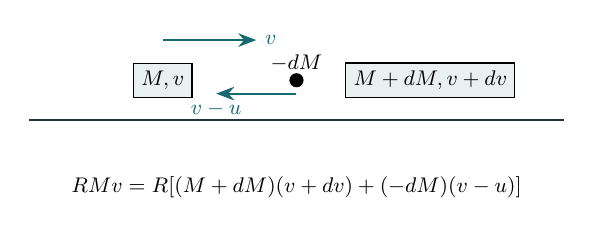
\begin{tikzpicture}[scale=.85,transform shape]

\draw[object] (-2,0)--(6,0);
\node[draw,fill=accent!10] at (0,.6) {$M,v$};
\draw[motion] (0,1.2)--(1.4,1.2) node[right] {$v$};
\node[draw,fill=accent!10] at (4,.6) {$M+dM,v+dv$};
\fill (2,.6) circle (3pt) node[above] {$-dM$};
\draw[motion] (2,.4)--(.8,.4) node[below] {$v-u$};
\node at (2,-1) {$RMv=R[(M+dM)(v+dv)+(-dM)(v-u)]$};

\end{tikzpicture}
\figcaption{解图综四.4A\quad 局部切向发射微元，但守恒式使用关于同一环心的角动量。}
\end{minipage}\end{center}
解图综四.4A取一个极短发射过程。装置连同待发珠的瞬时质量为$M$、正向速率为$v$，射出珠质量$-dM>0$；到一阶，珠相对圆环的有向速度为$v-u$。发射前后关于环心的角动量守恒：
\[
RMv=R[(M+dM)(v+dv)+(-dM)(v-u)].
\]
略去二阶小量$dM\,dv$，得到
\[
M\,dv+u\,dM=0,\qquad
dv=-u\frac{dM}{M}.
\]
若质量流率为$\mu$，则$\mu T=m$，且
$M(t)=2m-\mu t$。从$M(0)=2m,v(0)=0$积分，
\[
\boxed{v(t)=u\ln\frac{2m}{2m-\mu t}},\qquad 0\le t\le T.
\]
因而末速$v(T)=u\ln2<u$；所有发出的珠都逆着装置的正方向运动，速率在$u(1-\ln2)$与$u$之间。
\begin{center}\begin{minipage}{.98\linewidth}\centering
\begin{tikzpicture}[scale=.85,transform shape]

\draw[axis] (0,0)--(6,0) node[right] {$t/T$};
\draw[axis] (0,0)--(0,3.5) node[above] {弧长$/uT$};
\draw[traj,domain=0:1,samples=100] plot ({5*\x},{3*(\x+(2-\x)*ln(1-\x/2))});
\draw[object] (0,0)--(5,3) node[right] {$\ell_0/uT=t/T$};
\draw[guide] (5,0)--(5,3);
\node[below] at (5,0) {$1$};
\node[above left] at (5,.92056) {$\ell_P/uT=1-\ln2$};
\node at (3,-1.3) {$\ell_P(T)+\ell_0(T)=2\pi R$};

\end{tikzpicture}
\figcaption{解图综四.4B\quad 装置弧长由变速积分得到，第一珠逆向弧长随时间线性增长。}
\end{minipage}\end{center}
解图综四.4B以展开的圆周弧长记录两种运动。装置发射期间的路程为
\[
\ell_P=\int_0^T v(t)dt
=\frac u\mu\int_m^{2m}\ln\frac{2m}{M}\,dM.
\]
被积函数的原函数是$M[\ln(2m/M)+1]$，因此
\[
\ell_P=\frac u\mu\{2m-m(1+\ln2)\}
=\boxed{uT(1-\ln2)}.
\]
第一颗珠在$t=0$发出，装置初速零，故珠以逆向恒速$u$运动，至$T$的路程为$\ell_0=uT$。
题设首次迎头相遇对应两者相向走完一周：
\[
\ell_P+\ell_0=uT(2-\ln2)=2\pi R.
\]
故装置转角为
\[
\boxed{\theta=\frac{\ell_P}{R}
=2\pi\frac{1-\ln2}{2-\ln2}
=360^\circ\frac{1-\ln2}{2-\ln2}
\simeq85^\circ}.
\]
这里按题设取整到度；装置一直加速，图B在$t=T$处的弧长纵坐标给出实际路程。

确定首次迎头相遇，需要比较先后发出的珠子。对于在$\tau$发出的珠，到$t>\tau$与装置累积的相向弧长为
\[
D(t,\tau)=\ell_P(t)-\ell_P(\tau)
+[u-v(\tau)](t-\tau).
\]
对固定$t$求导：
\[
\frac{\partial D}{\partial\tau}
=-u-v'(\tau)(t-\tau)<0.
\]
所以先发的珠累积闭合路程更大，第一珠先达到$2\pi R$，没有后发珠在$T$前先绕回迎头碰到装置。此处不把珠刚离开尾部的接触算作迎头相遇。
\begin{center}\begin{minipage}{.98\linewidth}\centering
\begin{tikzpicture}[scale=.8,transform shape]

\draw[object] (0,0) circle (2);
\fill[accent] (-.3,1.88) rectangle (.3,2.12);
\node[above] at (0,2.2) {$P$};
\draw[motion] (.4,2)--(1.3,2) node[right] {$v$正向};
\draw[motion] (-.4,2)--(-1.3,2) node[left] {喷珠};
\fill (0,0) circle (2pt) node[below] {$O$};
\draw[guide] (0,0)--(1.414,-1.414) node[midway,below left] {$R$};

\foreach \ang in {15,40,70,110,140,170,200,230,270,300,330}{
\fill[warm] (\ang:1.9) circle (1.4pt);}
\node[align=left] at (5.5,.5) {所有游离珠逆行\\$w_i\ge u(1-\ln2)>0$\\$M_Pv=\sum m_iw_i>0$};
\node at (2,-3) {尚未全部回收时装置保持正行；收完后总角动量零};

\end{tikzpicture}
\figcaption{解图综四.4C\quad 回收阶段的正负角动量；非弹性吞入不守恒机械能。}
\end{minipage}\end{center}
第（2）问，解图综四.4C中$T$后停止发射，珠被装置吞入且不再离开。只要还有游离珠，它们都以非零逆向速率运动，最慢的也有
$w_{\min}=u(1-\ln2)>0$。记尚未吞入各珠质量为$m_i$、逆向速率为$w_i$，装置及已吞珠的总质量为$M_P$。总角动量零给
\[
RM_Pv-R\sum_{\rm free}m_iw_i=0,
\quad
\boxed{v=\frac{\sum_{\rm free}m_iw_i}{M_P}>0}.
\]
因此装置在尚未收完珠时保持正向运动，而每颗未收珠持续逆行，相对闭合速率不小于$w_{\min}$。每颗珠最多再走一个相对圆周就必遇到装置，所以在有限时间内能全部收回。

全部回收后总质量为$2m$，系统只剩同一装置的圆周运动。角动量守恒给
\[
2mR\,v_\infty=0,\qquad \boxed{v_\infty=0}.
\]
吞入是非弹性过程，会耗散动能。末态由关于环心的角动量确定，吞入中损失的动能转为内能。

\textbf{发射与回收的完整时间图像。} 解图综四.4D以$x=t/T$为横坐标，将装置与各批珠子的运动画在同一圆周展开坐标中。质量微元$\mu\,dt$离开后，在光滑圆环上只受径向支持力，因此其关于环心的角动量$R\,dm\,w$保持不变，圆环参考系中的有向切向速度$w=v(\tau)-u$也保持不变。珠子的切线方向虽随位置转动，每颗珠子的有向弧长仍随时间线性变化；这正是展开图中各条珠子轨迹为直线的理由。
\begin{center}\begin{minipage}{.98\linewidth}\centering
\begin{tikzpicture}[scale=0.72,transform shape]
\draw[axis] (0,0)--(6.2,0);\draw[axis] (0,0)--(0,3.4000000000000004);
\draw[thin,color=muted] (0.0000000,0)--(0.0000000,-.07);\node[below] at (0.0000000,-.09) {$0$};
\draw[thin,color=muted] (3.0000000,0)--(3.0000000,-.07);\node[below] at (3.0000000,-.09) {$.5$};
\draw[thin,color=muted] (6.0000000,0)--(6.0000000,-.07);\node[below] at (6.0000000,-.09) {$1$};
\draw[thin,color=muted] (0,0.1142857)--(-.07,0.1142857);\node[left] at (-.09,0.1142857) {$-1$};
\draw[thin,color=muted] (0,2.4000000)--(-.07,2.4000000);\node[left] at (-.09,2.4000000) {$0$};
\draw[thin,color=muted] (0,3.0857143)--(-.07,3.0857143);\node[left] at (-.09,3.0857143) {$.3$};
\node[below] at (3.0,-.64) {$t/T$};\node[above right] at (0,3.45) {有向弧长除以uT};
\draw[traj] plot coordinates {(0.0000000,2.4000000) (0.0250000,2.4000099) (0.0500000,2.4000397) (0.0750000,2.4000895) (0.1000000,2.4001592) (0.1250000,2.4002489) (0.1500000,2.4003586) (0.1750000,2.4004885) (0.2000000,2.4006385) (0.2250000,2.4008086) (0.2500000,2.4009990) (0.2750000,2.4012097) (0.3000000,2.4014406) (0.3250000,2.4016919) (0.3500000,2.4019636) (0.3750000,2.4022558) (0.4000000,2.4025684) (0.4250000,2.4029015) (0.4500000,2.4032552) (0.4750000,2.4036296) (0.5000000,2.4040245) (0.5250000,2.4044402) (0.5500000,2.4048767) (0.5750000,2.4053339) (0.6000000,2.4058120) (0.6250000,2.4063109) (0.6500000,2.4068308) (0.6750000,2.4073717) (0.7000000,2.4079336) (0.7250000,2.4085165) (0.7500000,2.4091206) (0.7750000,2.4097459) (0.8000000,2.4103923) (0.8250000,2.4110600) (0.8500000,2.4117491) (0.8750000,2.4124594) (0.9000000,2.4131912) (0.9250000,2.4139444) (0.9500000,2.4147191) (0.9750000,2.4155154) (1.0000000,2.4163333) (1.0250000,2.4171728) (1.0500000,2.4180340) (1.0750000,2.4189169) (1.1000000,2.4198217) (1.1250000,2.4207483) (1.1500000,2.4216967) (1.1750000,2.4226672) (1.2000000,2.4236596) (1.2250000,2.4246741) (1.2500000,2.4257106) (1.2750000,2.4267693) (1.3000000,2.4278502) (1.3250000,2.4289534) (1.3500000,2.4300789) (1.3750000,2.4312267) (1.4000000,2.4323969) (1.4250000,2.4335896) (1.4500000,2.4348048) (1.4750000,2.4360426) (1.5000000,2.4373030) (1.5250000,2.4385861) (1.5500000,2.4398919) (1.5750000,2.4412205) (1.6000000,2.4425719) (1.6250000,2.4439462) (1.6500000,2.4453435) (1.6750000,2.4467638) (1.7000000,2.4482071) (1.7250000,2.4496735) (1.7500000,2.4511632) (1.7750000,2.4526760) (1.8000000,2.4542122) (1.8250000,2.4557716) (1.8500000,2.4573545) (1.8750000,2.4589609) (1.9000000,2.4605907) (1.9250000,2.4622441) (1.9500000,2.4639212) (1.9750000,2.4656219) (2.0000000,2.4673465) (2.0250000,2.4690948) (2.0500000,2.4708669) (2.0750000,2.4726630) (2.1000000,2.4744831) (2.1250000,2.4763273) (2.1500000,2.4781956) (2.1750000,2.4800880) (2.2000000,2.4820047) (2.2250000,2.4839456) (2.2500000,2.4859109) (2.2750000,2.4879007) (2.3000000,2.4899149) (2.3250000,2.4919537) (2.3500000,2.4940170) (2.3750000,2.4961051) (2.4000000,2.4982179) (2.4250000,2.5003555) (2.4500000,2.5025179) (2.4750000,2.5047053) (2.5000000,2.5069177) (2.5250000,2.5091551) (2.5500000,2.5114177) (2.5750000,2.5137055) (2.6000000,2.5160185) (2.6250000,2.5183569) (2.6500000,2.5207206) (2.6750000,2.5231098) (2.7000000,2.5255246) (2.7250000,2.5279650) (2.7500000,2.5304310) (2.7750000,2.5329228) (2.8000000,2.5354403) (2.8250000,2.5379838) (2.8500000,2.5405532) (2.8750000,2.5431486) (2.9000000,2.5457702) (2.9250000,2.5484178) (2.9500000,2.5510918) (2.9750000,2.5537920) (3.0000000,2.5565186) (3.0250000,2.5592717) (3.0500000,2.5620513) (3.0750000,2.5648575) (3.1000000,2.5676904) (3.1250000,2.5705500) (3.1500000,2.5734364) (3.1750000,2.5763498) (3.2000000,2.5792901) (3.2250000,2.5822575) (3.2500000,2.5852521) (3.2750000,2.5882738) (3.3000000,2.5913228) (3.3250000,2.5943992) (3.3500000,2.5975031) (3.3750000,2.6006345) (3.4000000,2.6037934) (3.4250000,2.6069801) (3.4500000,2.6101945) (3.4750000,2.6134368) (3.5000000,2.6167070) (3.5250000,2.6200052) (3.5500000,2.6233315) (3.5750000,2.6266860) (3.6000000,2.6300688) (3.6250000,2.6334798) (3.6500000,2.6369194) (3.6750000,2.6403874) (3.7000000,2.6438840) (3.7250000,2.6474094) (3.7500000,2.6509634) (3.7750000,2.6545464) (3.8000000,2.6581583) (3.8250000,2.6617992) (3.8500000,2.6654693) (3.8750000,2.6691686) (3.9000000,2.6728972) (3.9250000,2.6766551) (3.9500000,2.6804426) (3.9750000,2.6842596) (4.0000000,2.6881063) (4.0250000,2.6919828) (4.0500000,2.6958891) (4.0750000,2.6998254) (4.1000000,2.7037917) (4.1250000,2.7077882) (4.1500000,2.7118149) (4.1750000,2.7158719) (4.2000000,2.7199593) (4.2250000,2.7240773) (4.2500000,2.7282259) (4.2750000,2.7324052) (4.3000000,2.7366154) (4.3250000,2.7408564) (4.3500000,2.7451285) (4.3750000,2.7494317) (4.4000000,2.7537661) (4.4250000,2.7581319) (4.4500000,2.7625291) (4.4750000,2.7669578) (4.5000000,2.7714182) (4.5250000,2.7759103) (4.5500000,2.7804343) (4.5750000,2.7849902) (4.6000000,2.7895782) (4.6250000,2.7941984) (4.6500000,2.7988508) (4.6750000,2.8035357) (4.7000000,2.8082530) (4.7250000,2.8130030) (4.7500000,2.8177857) (4.7750000,2.8226012) (4.8000000,2.8274497) (4.8250000,2.8323313) (4.8500000,2.8372460) (4.8750000,2.8421941) (4.9000000,2.8471755) (4.9250000,2.8521905) (4.9500000,2.8572392) (4.9750000,2.8623216) (5.0000000,2.8674379) (5.0250000,2.8725882) (5.0500000,2.8777727) (5.0750000,2.8829914) (5.1000000,2.8882445) (5.1250000,2.8935321) (5.1500000,2.8988544) (5.1750000,2.9042114) (5.2000000,2.9096033) (5.2250000,2.9150302) (5.2500000,2.9204922) (5.2750000,2.9259895) (5.3000000,2.9315222) (5.3250000,2.9370905) (5.3500000,2.9426944) (5.3750000,2.9483342) (5.4000000,2.9540098) (5.4250000,2.9597216) (5.4500000,2.9654695) (5.4750000,2.9712538) (5.5000000,2.9770746) (5.5250000,2.9829321) (5.5500000,2.9888263) (5.5750000,2.9947574) (5.6000000,3.0007256) (5.6250000,3.0067309) (5.6500000,3.0127737) (5.6750000,3.0188539) (5.7000000,3.0249717) (5.7250000,3.0311274) (5.7500000,3.0373210) (5.7750000,3.0435527) (5.8000000,3.0498226) (5.8250000,3.0561310) (5.8500000,3.0624779) (5.8750000,3.0688635) (5.9000000,3.0752880) (5.9250000,3.0817515) (5.9500000,3.0882542) (5.9750000,3.0947963) (6.0000000,3.1013779)};
\draw[traj] (.1,-1.05)--(.7,-1.05);\node[right] at (.85,-1.05) {装置弧长};\draw[dashed,thick,color=warm] plot coordinates {(0.0000000,2.4000000) (0.0400000,2.3847619) (0.0800000,2.3695238) (0.1200000,2.3542857) (0.1600000,2.3390476) (0.2000000,2.3238095) (0.2400000,2.3085714) (0.2800000,2.2933333) (0.3200000,2.2780952) (0.3600000,2.2628571) (0.4000000,2.2476190) (0.4400000,2.2323810) (0.4800000,2.2171429) (0.5200000,2.2019048) (0.5600000,2.1866667) (0.6000000,2.1714286) (0.6400000,2.1561905) (0.6800000,2.1409524) (0.7200000,2.1257143) (0.7600000,2.1104762) (0.8000000,2.0952381) (0.8400000,2.0800000) (0.8800000,2.0647619) (0.9200000,2.0495238) (0.9600000,2.0342857) (1.0000000,2.0190476) (1.0400000,2.0038095) (1.0800000,1.9885714) (1.1200000,1.9733333) (1.1600000,1.9580952) (1.2000000,1.9428571) (1.2400000,1.9276190) (1.2800000,1.9123810) (1.3200000,1.8971429) (1.3600000,1.8819048) (1.4000000,1.8666667) (1.4400000,1.8514286) (1.4800000,1.8361905) (1.5200000,1.8209524) (1.5600000,1.8057143) (1.6000000,1.7904762) (1.6400000,1.7752381) (1.6800000,1.7600000) (1.7200000,1.7447619) (1.7600000,1.7295238) (1.8000000,1.7142857) (1.8400000,1.6990476) (1.8800000,1.6838095) (1.9200000,1.6685714) (1.9600000,1.6533333) (2.0000000,1.6380952) (2.0400000,1.6228571) (2.0800000,1.6076190) (2.1200000,1.5923810) (2.1600000,1.5771429) (2.2000000,1.5619048) (2.2400000,1.5466667) (2.2800000,1.5314286) (2.3200000,1.5161905) (2.3600000,1.5009524) (2.4000000,1.4857143) (2.4400000,1.4704762) (2.4800000,1.4552381) (2.5200000,1.4400000) (2.5600000,1.4247619) (2.6000000,1.4095238) (2.6400000,1.3942857) (2.6800000,1.3790476) (2.7200000,1.3638095) (2.7600000,1.3485714) (2.8000000,1.3333333) (2.8400000,1.3180952) (2.8800000,1.3028571) (2.9200000,1.2876190) (2.9600000,1.2723810) (3.0000000,1.2571429) (3.0400000,1.2419048) (3.0800000,1.2266667) (3.1200000,1.2114286) (3.1600000,1.1961905) (3.2000000,1.1809524) (3.2400000,1.1657143) (3.2800000,1.1504762) (3.3200000,1.1352381) (3.3600000,1.1200000) (3.4000000,1.1047619) (3.4400000,1.0895238) (3.4800000,1.0742857) (3.5200000,1.0590476) (3.5600000,1.0438095) (3.6000000,1.0285714) (3.6400000,1.0133333) (3.6800000,0.9980952) (3.7200000,0.9828571) (3.7600000,0.9676190) (3.8000000,0.9523810) (3.8400000,0.9371429) (3.8800000,0.9219048) (3.9200000,0.9066667) (3.9600000,0.8914286) (4.0000000,0.8761905) (4.0400000,0.8609524) (4.0800000,0.8457143) (4.1200000,0.8304762) (4.1600000,0.8152381) (4.2000000,0.8000000) (4.2400000,0.7847619) (4.2800000,0.7695238) (4.3200000,0.7542857) (4.3600000,0.7390476) (4.4000000,0.7238095) (4.4400000,0.7085714) (4.4800000,0.6933333) (4.5200000,0.6780952) (4.5600000,0.6628571) (4.6000000,0.6476190) (4.6400000,0.6323810) (4.6800000,0.6171429) (4.7200000,0.6019048) (4.7600000,0.5866667) (4.8000000,0.5714286) (4.8400000,0.5561905) (4.8800000,0.5409524) (4.9200000,0.5257143) (4.9600000,0.5104762) (5.0000000,0.4952381) (5.0400000,0.4800000) (5.0800000,0.4647619) (5.1200000,0.4495238) (5.1600000,0.4342857) (5.2000000,0.4190476) (5.2400000,0.4038095) (5.2800000,0.3885714) (5.3200000,0.3733333) (5.3600000,0.3580952) (5.4000000,0.3428571) (5.4400000,0.3276190) (5.4800000,0.3123810) (5.5200000,0.2971429) (5.5600000,0.2819048) (5.6000000,0.2666667) (5.6400000,0.2514286) (5.6800000,0.2361905) (5.7200000,0.2209524) (5.7600000,0.2057143) (5.8000000,0.1904762) (5.8400000,0.1752381) (5.8800000,0.1600000) (5.9200000,0.1447619) (5.9600000,0.1295238) (6.0000000,0.1142857)};
\draw[dashed,thick,color=warm] (.1,-1.48)--(.7,-1.48);\node[right] at (.85,-1.48) {发射时刻$\tau/T=0$的珠};\draw[dotted,thick,color=muted] plot coordinates {(1.8000000,2.4542122) (1.8280000,2.4452790) (1.8560000,2.4363459) (1.8840000,2.4274128) (1.9120000,2.4184796) (1.9400000,2.4095465) (1.9680000,2.4006134) (1.9960000,2.3916802) (2.0240000,2.3827471) (2.0520000,2.3738140) (2.0800000,2.3648808) (2.1080000,2.3559477) (2.1360000,2.3470146) (2.1640000,2.3380815) (2.1920000,2.3291483) (2.2200000,2.3202152) (2.2480000,2.3112821) (2.2760000,2.3023489) (2.3040000,2.2934158) (2.3320000,2.2844827) (2.3600000,2.2755495) (2.3880000,2.2666164) (2.4160000,2.2576833) (2.4440000,2.2487501) (2.4720000,2.2398170) (2.5000000,2.2308839) (2.5280000,2.2219507) (2.5560000,2.2130176) (2.5840000,2.2040845) (2.6120000,2.1951513) (2.6400000,2.1862182) (2.6680000,2.1772851) (2.6960000,2.1683520) (2.7240000,2.1594188) (2.7520000,2.1504857) (2.7800000,2.1415526) (2.8080000,2.1326194) (2.8360000,2.1236863) (2.8640000,2.1147532) (2.8920000,2.1058200) (2.9200000,2.0968869) (2.9480000,2.0879538) (2.9760000,2.0790206) (3.0040000,2.0700875) (3.0320000,2.0611544) (3.0600000,2.0522212) (3.0880000,2.0432881) (3.1160000,2.0343550) (3.1440000,2.0254219) (3.1720000,2.0164887) (3.2000000,2.0075556) (3.2280000,1.9986225) (3.2560000,1.9896893) (3.2840000,1.9807562) (3.3120000,1.9718231) (3.3400000,1.9628899) (3.3680000,1.9539568) (3.3960000,1.9450237) (3.4240000,1.9360905) (3.4520000,1.9271574) (3.4800000,1.9182243) (3.5080000,1.9092911) (3.5360000,1.9003580) (3.5640000,1.8914249) (3.5920000,1.8824917) (3.6200000,1.8735586) (3.6480000,1.8646255) (3.6760000,1.8556924) (3.7040000,1.8467592) (3.7320000,1.8378261) (3.7600000,1.8288930) (3.7880000,1.8199598) (3.8160000,1.8110267) (3.8440000,1.8020936) (3.8720000,1.7931604) (3.9000000,1.7842273) (3.9280000,1.7752942) (3.9560000,1.7663610) (3.9840000,1.7574279) (4.0120000,1.7484948) (4.0400000,1.7395616) (4.0680000,1.7306285) (4.0960000,1.7216954) (4.1240000,1.7127623) (4.1520000,1.7038291) (4.1800000,1.6948960) (4.2080000,1.6859629) (4.2360000,1.6770297) (4.2640000,1.6680966) (4.2920000,1.6591635) (4.3200000,1.6502303) (4.3480000,1.6412972) (4.3760000,1.6323641) (4.4040000,1.6234309) (4.4320000,1.6144978) (4.4600000,1.6055647) (4.4880000,1.5966315) (4.5160000,1.5876984) (4.5440000,1.5787653) (4.5720000,1.5698321) (4.6000000,1.5608990) (4.6280000,1.5519659) (4.6560000,1.5430328) (4.6840000,1.5340996) (4.7120000,1.5251665) (4.7400000,1.5162334) (4.7680000,1.5073002) (4.7960000,1.4983671) (4.8240000,1.4894340) (4.8520000,1.4805008) (4.8800000,1.4715677) (4.9080000,1.4626346) (4.9360000,1.4537014) (4.9640000,1.4447683) (4.9920000,1.4358352) (5.0200000,1.4269020) (5.0480000,1.4179689) (5.0760000,1.4090358) (5.1040000,1.4001027) (5.1320000,1.3911695) (5.1600000,1.3822364) (5.1880000,1.3733033) (5.2160000,1.3643701) (5.2440000,1.3554370) (5.2720000,1.3465039) (5.3000000,1.3375707) (5.3280000,1.3286376) (5.3560000,1.3197045) (5.3840000,1.3107713) (5.4120000,1.3018382) (5.4400000,1.2929051) (5.4680000,1.2839719) (5.4960000,1.2750388) (5.5240000,1.2661057) (5.5520000,1.2571725) (5.5800000,1.2482394) (5.6080000,1.2393063) (5.6360000,1.2303732) (5.6640000,1.2214400) (5.6920000,1.2125069) (5.7200000,1.2035738) (5.7480000,1.1946406) (5.7760000,1.1857075) (5.8040000,1.1767744) (5.8320000,1.1678412) (5.8600000,1.1589081) (5.8880000,1.1499750) (5.9160000,1.1410418) (5.9440000,1.1321087) (5.9720000,1.1231756) (6.0000000,1.1142424)};
\draw[dotted,thick,color=muted] (.1,-1.9100000000000001)--(.7,-1.9100000000000001);\node[right] at (.85,-1.9100000000000001) {发射时刻$\tau/T=0.3$的珠};\draw[dash dot,thick,color=ink] plot coordinates {(3.9000000,2.6728972) (3.9140000,2.6696601) (3.9280000,2.6664229) (3.9420000,2.6631858) (3.9560000,2.6599487) (3.9700000,2.6567116) (3.9840000,2.6534745) (3.9980000,2.6502374) (4.0120000,2.6470003) (4.0260000,2.6437632) (4.0400000,2.6405261) (4.0540000,2.6372890) (4.0680000,2.6340519) (4.0820000,2.6308148) (4.0960000,2.6275777) (4.1100000,2.6243406) (4.1240000,2.6211035) (4.1380000,2.6178664) (4.1520000,2.6146292) (4.1660000,2.6113921) (4.1800000,2.6081550) (4.1940000,2.6049179) (4.2080000,2.6016808) (4.2220000,2.5984437) (4.2360000,2.5952066) (4.2500000,2.5919695) (4.2640000,2.5887324) (4.2780000,2.5854953) (4.2920000,2.5822582) (4.3060000,2.5790211) (4.3200000,2.5757840) (4.3340000,2.5725469) (4.3480000,2.5693098) (4.3620000,2.5660727) (4.3760000,2.5628355) (4.3900000,2.5595984) (4.4040000,2.5563613) (4.4180000,2.5531242) (4.4320000,2.5498871) (4.4460000,2.5466500) (4.4600000,2.5434129) (4.4740000,2.5401758) (4.4880000,2.5369387) (4.5020000,2.5337016) (4.5160000,2.5304645) (4.5300000,2.5272274) (4.5440000,2.5239903) (4.5580000,2.5207532) (4.5720000,2.5175161) (4.5860000,2.5142790) (4.6000000,2.5110418) (4.6140000,2.5078047) (4.6280000,2.5045676) (4.6420000,2.5013305) (4.6560000,2.4980934) (4.6700000,2.4948563) (4.6840000,2.4916192) (4.6980000,2.4883821) (4.7120000,2.4851450) (4.7260000,2.4819079) (4.7400000,2.4786708) (4.7540000,2.4754337) (4.7680000,2.4721966) (4.7820000,2.4689595) (4.7960000,2.4657224) (4.8100000,2.4624853) (4.8240000,2.4592481) (4.8380000,2.4560110) (4.8520000,2.4527739) (4.8660000,2.4495368) (4.8800000,2.4462997) (4.8940000,2.4430626) (4.9080000,2.4398255) (4.9220000,2.4365884) (4.9360000,2.4333513) (4.9500000,2.4301142) (4.9640000,2.4268771) (4.9780000,2.4236400) (4.9920000,2.4204029) (5.0060000,2.4171658) (5.0200000,2.4139287) (5.0340000,2.4106916) (5.0480000,2.4074544) (5.0620000,2.4042173) (5.0760000,2.4009802) (5.0900000,2.3977431) (5.1040000,2.3945060) (5.1180000,2.3912689) (5.1320000,2.3880318) (5.1460000,2.3847947) (5.1600000,2.3815576) (5.1740000,2.3783205) (5.1880000,2.3750834) (5.2020000,2.3718463) (5.2160000,2.3686092) (5.2300000,2.3653721) (5.2440000,2.3621350) (5.2580000,2.3588979) (5.2720000,2.3556607) (5.2860000,2.3524236) (5.3000000,2.3491865) (5.3140000,2.3459494) (5.3280000,2.3427123) (5.3420000,2.3394752) (5.3560000,2.3362381) (5.3700000,2.3330010) (5.3840000,2.3297639) (5.3980000,2.3265268) (5.4120000,2.3232897) (5.4260000,2.3200526) (5.4400000,2.3168155) (5.4540000,2.3135784) (5.4680000,2.3103413) (5.4820000,2.3071042) (5.4960000,2.3038671) (5.5100000,2.3006299) (5.5240000,2.2973928) (5.5380000,2.2941557) (5.5520000,2.2909186) (5.5660000,2.2876815) (5.5800000,2.2844444) (5.5940000,2.2812073) (5.6080000,2.2779702) (5.6220000,2.2747331) (5.6360000,2.2714960) (5.6500000,2.2682589) (5.6640000,2.2650218) (5.6780000,2.2617847) (5.6920000,2.2585476) (5.7060000,2.2553105) (5.7200000,2.2520734) (5.7340000,2.2488362) (5.7480000,2.2455991) (5.7620000,2.2423620) (5.7760000,2.2391249) (5.7900000,2.2358878) (5.8040000,2.2326507) (5.8180000,2.2294136) (5.8320000,2.2261765) (5.8460000,2.2229394) (5.8600000,2.2197023) (5.8740000,2.2164652) (5.8880000,2.2132281) (5.9020000,2.2099910) (5.9160000,2.2067539) (5.9300000,2.2035168) (5.9440000,2.2002797) (5.9580000,2.1970425) (5.9720000,2.1938054) (5.9860000,2.1905683) (6.0000000,2.1873312)};
\draw[dash dot,thick,color=ink] (.1,-2.34)--(.7,-2.34);\node[right] at (.85,-2.34) {发射时刻$\tau/T=0.65$的珠};\end{tikzpicture}
\figcaption{解图综四.4D\quad 圆周展开后，装置加速前进，各批珠沿不同斜率的直线逆行}
\end{minipage}\end{center}
装置的正向加速度为
\[
\dot v=\frac{u\mu}{2m-\mu t}>0,\qquad
\dot v(0)=\frac{u}{2T},\quad \dot v(T)=\frac uT.
\]
因此其弧长曲线先缓后陡。把速度积分中的变量换成剩余质量$M$，利用$dt=-dM/\mu$，就把变速过程转为从$m$到$2m$的定限积分。也可直接令$z=2-t/T$，保留每一步积分：
\[
\frac{\ell_P(t)}{uT}
=\int_0^{t/T}\ln\frac2{2-x}\,dx
=\frac tT+\left(2-\frac tT\right)\ln\left(1-\frac t{2T}\right).
\]
这里用到$\int\ln z\,dz=z\ln z-z$。在$t=T$处得$1-\ln2$，与质量积分的结果一致。平均速率为$u(1-\ln2)$，小于末速$u\ln2$，反映装置在发射中一直加速。

解图D中第$\tau$批珠子的直线从装置在$\tau$时刻的位置开始，斜率为$v(\tau)-u$。第一珠的直线从原点出发且最陡向下，其与装置曲线在展开坐标中的竖直间距，到$T$恰为一周。相遇排序式中的$\partial D/\partial\tau<0$同时包含两种作用：较晚发出的珠少走了时间，装置在它发出时的正向速度又较大，使其逆向速度较小。所以发射结束前一直没有绕回的珠进入头部，发射方程在整个$0<t<T$内都适用。

转角也可由两段弧长所对应的圆心角直接相除。令第一珠逆行的角度为$\theta_0$，则
\[
\frac{\theta}{\theta_0}
=\frac{\ell_P}{\ell_0}=1-\ln2=\ln(e/2),
\qquad \theta+\theta_0=2\pi.
\]
这两个几何关系消去$\theta_0$，恰好得到前面的角度。图B与图D的弧长纵坐标采用同一个$uT$作为单位，装置前进部分和第一珠逆行部分首尾接成完整圆周。

回收证明还给出了一个统一的有限时间上限。$T$时刻任意游离珠与装置之间沿相向闭合方向的间隔不超过$2\pi R$；此后只要它尚未进入头部，珠的逆速至少为$u(1-\ln2)$，而装置正向速率非负。因此全部回收所需的额外时间满足
\[
t_{\rm collect}\leqslant\frac{2\pi R}{u(1-\ln2)}
=T\,\frac{2-\ln2}{1-\ln2}.
\]
这是保守上限，装置向前迎接珠子使实际闭合更快。无论某一批珠子何时进入头部，吸收都将同一位置的质量合并，关于环心的角动量连续守恒。若碰前装置质量为$M_P$、速度为$v$，进入质量$\delta m$、逆速$w$，则碰后正向速度为$(M_Pv-\delta m\,w)/(M_P+\delta m)$。尚有游离珠时，总角动量所给的正值表达式继续成立；最后一批进入后，正负角动量恰好抵消，装置停下。


\Needspace{8\baselineskip}

\pdfbookmark[3]{关键洞察}{q4-h5}

\subsection*{关键洞察}

\begin{itemize}
\item 恒定的是相对喷速和质量流率，装置加速度为$u\mu/M$，随着$M$减小而增大。用末速乘总时间会高估装置弧长。
\item 第一珠最先回来同时由发射时刻与逆向速度决定。$\partial D/\partial\tau=-u-v'(\tau)(t-\tau)$把这两种影响写成同号的两项，给出完整排序。
\item $v(T)<u$保证全部珠逆行；再由总角动量零保证装置在尚有游离珠时正行。两者共同使“全部回收”成为可达到的结果。
\end{itemize}

\Needspace{8\baselineskip}

\pdfbookmark[3]{易错点}{q4-h6}

\subsection*{易错点}

\begin{itemize}
\item 用$u$代替每颗珠相对圆环的速率会丢失装置的发射瞬时速度；仅第一珠的逆速恰为$u$。图D中后发直线的斜率绝对值逐渐减小。
\item 系统受圆环的径向外力，使用总线动量守恒会混淆不同位置的切向方向。整个过程适用的是对固定环心的角动量守恒。
\item 图B中两段弧长相向，和为周长；装置弧长是速度曲线下的面积。将两段相减会错置相遇位置，取末速乘$T$则高估这个面积。
\item 吞入使珠留在装置内，属于非弹性吸收。回收计算保留角动量，动能差转为内能；发射时的动能由装置内部供能提供。
\end{itemize}

\Needspace{8\baselineskip}

\pdfbookmark[3]{课堂讲解建议}{q4-h7}

\subsection*{课堂讲解建议}

\begin{itemize}
\item 让学生在圆轨道上选两个相隔较远的位置，分别画径向支持力和局部切线。追问径向力对线动量与对环心角动量的作用，学生说明径向力改变线动量、对环心力矩为零，因而系统对环心的总角动量守恒。
\item 在图A先问“尾部刚离开的珠在圆环系中速度是多少”，学生回答$v-u$，再列一个微元过程。积分后用图B讨论平均速率与末速的大小，并让学生以质量为变量独立完成定限积分。
\item 画两颗先后发出的珠，比较它们的出发时刻、出发位置和逆速。将这些直觉写成$D(t,\tau)$，对$\tau$求导解释哪颗先迎头返回。
\item 回收时先假设还有一小批珠在外，让学生给总角动量各项标正负。追问装置此时能否停下，学生由游离珠负角动量和总角动量零说明装置仍正行。由装置正行和珠逆行讨论有限相遇时间，再算最后一次吸收，衔接末速零的结论。
\end{itemize}

\Needspace{8\baselineskip}

\pdfbookmark[3]{变式训练}{q4-h8}

\subsection*{变式训练}

\begin{enumerate}
\Needspace{37\baselineskip}
\item \textbf{题设与求解。} 珠总质量改为$bm$、干质量为$m$，取$0<b<e-1$，仍在发完时首次相遇。初始质量$(1+b)m$，$T=bm/\mu$，故$v_f=u\ln(1+b)$。质量积分给$\ell_P=(um/\mu)[b-\ln(1+b)]$，记$A_b=1-\ln(1+b)/b$，则$\ell_P=uTA_b$。第一珠仍走$uT$，从而
\[
\theta=2\pi\frac{A_b}{1+A_b},\qquad uT=\frac{2\pi R}{1+A_b}.
\]
图V1画$\theta$随$b$的变化。所取$b$使$v_f<u$，全部游离珠逆行，主解的正负角动量证明给出全部回收后的速率零。质量比增大时，装置在发射期间的平均速率增大，前进弧长占一周的比例也增大。
\begin{center}\begin{minipage}{.98\linewidth}\centering
\begin{tikzpicture}[scale=0.72,transform shape]
\draw[axis] (0,0)--(6.2,0);\draw[axis] (0,0)--(0,3.4000000000000004);
\draw[thin,color=muted] (0.0000000,0)--(0.0000000,-.07);\node[below] at (0.0000000,-.09) {$0$};
\draw[thin,color=muted] (3.4285714,0)--(3.4285714,-.07);\node[below] at (3.4285714,-.09) {$1$};
\draw[thin,color=muted] (5.8285714,0)--(5.8285714,-.07);\node[below] at (5.8285714,-.09) {$1.7$};
\draw[thin,color=muted] (0,0.0000000)--(-.07,0.0000000);\node[left] at (-.09,0.0000000) {$0$};
\draw[thin,color=muted] (0,1.4545455)--(-.07,1.4545455);\node[left] at (-.09,1.4545455) {$50$};
\draw[thin,color=muted] (0,2.9090909)--(-.07,2.9090909);\node[left] at (-.09,2.9090909) {$100$};
\node[below] at (3.0,-.64) {珠质量与干质量比b};\node[above right] at (0,3.45) {转角（度）};
\draw[traj] plot coordinates {(0.0342857,0.0517601) (0.0584286,0.0874981) (0.0825714,0.1226664) (0.1067143,0.1572790) (0.1308571,0.1913494) (0.1550000,0.2248908) (0.1791429,0.2579159) (0.2032857,0.2904371) (0.2274286,0.3224663) (0.2515714,0.3540150) (0.2757143,0.3850943) (0.2998571,0.4157151) (0.3240000,0.4458879) (0.3481429,0.4756229) (0.3722857,0.5049299) (0.3964286,0.5338184) (0.4205714,0.5622978) (0.4447143,0.5903770) (0.4688571,0.6180647) (0.4930000,0.6453695) (0.5171429,0.6722995) (0.5412857,0.6988628) (0.5654286,0.7250671) (0.5895714,0.7509199) (0.6137143,0.7764286) (0.6378571,0.8016003) (0.6620000,0.8264418) (0.6861429,0.8509600) (0.7102857,0.8751614) (0.7344286,0.8990523) (0.7585714,0.9226389) (0.7827143,0.9459273) (0.8068571,0.9689233) (0.8310000,0.9916327) (0.8551429,1.0140610) (0.8792857,1.0362135) (0.9034286,1.0580957) (0.9275714,1.0797126) (0.9517143,1.1010692) (0.9758571,1.1221704) (1.0000000,1.1430210) (1.0241429,1.1636256) (1.0482857,1.1839887) (1.0724286,1.2041147) (1.0965714,1.2240080) (1.1207143,1.2436727) (1.1448571,1.2631129) (1.1690000,1.2823327) (1.1931429,1.3013358) (1.2172857,1.3201261) (1.2414286,1.3387074) (1.2655714,1.3570833) (1.2897143,1.3752572) (1.3138571,1.3932327) (1.3380000,1.4110131) (1.3621429,1.4286018) (1.3862857,1.4460019) (1.4104286,1.4632167) (1.4345714,1.4802491) (1.4587143,1.4971023) (1.4828571,1.5137791) (1.5070000,1.5302824) (1.5311429,1.5466152) (1.5552857,1.5627800) (1.5794286,1.5787796) (1.6035714,1.5946167) (1.6277143,1.6102937) (1.6518571,1.6258134) (1.6760000,1.6411780) (1.7001429,1.6563901) (1.7242857,1.6714519) (1.7484286,1.6863659) (1.7725714,1.7011342) (1.7967143,1.7157592) (1.8208571,1.7302429) (1.8450000,1.7445876) (1.8691429,1.7587952) (1.8932857,1.7728679) (1.9174286,1.7868076) (1.9415714,1.8006164) (1.9657143,1.8142961) (1.9898571,1.8278486) (2.0140000,1.8412757) (2.0381429,1.8545794) (2.0622857,1.8677613) (2.0864286,1.8808232) (2.1105714,1.8937668) (2.1347143,1.9065938) (2.1588571,1.9193059) (2.1830000,1.9319046) (2.2071429,1.9443915) (2.2312857,1.9567681) (2.2554286,1.9690361) (2.2795714,1.9811969) (2.3037143,1.9932519) (2.3278571,2.0052026) (2.3520000,2.0170504) (2.3761429,2.0287968) (2.4002857,2.0404429) (2.4244286,2.0519903) (2.4485714,2.0634402) (2.4727143,2.0747939) (2.4968571,2.0860526) (2.5210000,2.0972177) (2.5451429,2.1082902) (2.5692857,2.1192715) (2.5934286,2.1301627) (2.6175714,2.1409650) (2.6417143,2.1516794) (2.6658571,2.1623072) (2.6900000,2.1728494) (2.7141429,2.1833071) (2.7382857,2.1936813) (2.7624286,2.2039731) (2.7865714,2.2141836) (2.8107143,2.2243137) (2.8348571,2.2343644) (2.8590000,2.2443367) (2.8831429,2.2542316) (2.9072857,2.2640500) (2.9314286,2.2737928) (2.9555714,2.2834609) (2.9797143,2.2930553) (3.0038571,2.3025768) (3.0280000,2.3120263) (3.0521429,2.3214046) (3.0762857,2.3307126) (3.1004286,2.3399512) (3.1245714,2.3491210) (3.1487143,2.3582230) (3.1728571,2.3672578) (3.1970000,2.3762264) (3.2211429,2.3851294) (3.2452857,2.3939676) (3.2694286,2.4027417) (3.2935714,2.4114526) (3.3177143,2.4201008) (3.3418571,2.4286870) (3.3660000,2.4372121) (3.3901429,2.4456767) (3.4142857,2.4540814) (3.4384286,2.4624269) (3.4625714,2.4707138) (3.4867143,2.4789429) (3.5108571,2.4871147) (3.5350000,2.4952299) (3.5591429,2.5032891) (3.5832857,2.5112928) (3.6074286,2.5192418) (3.6315714,2.5271365) (3.6557143,2.5349776) (3.6798571,2.5427656) (3.7040000,2.5505012) (3.7281429,2.5581847) (3.7522857,2.5658169) (3.7764286,2.5733982) (3.8005714,2.5809291) (3.8247143,2.5884103) (3.8488571,2.5958422) (3.8730000,2.6032253) (3.8971429,2.6105601) (3.9212857,2.6178471) (3.9454286,2.6250869) (3.9695714,2.6322798) (3.9937143,2.6394264) (4.0178571,2.6465272) (4.0420000,2.6535825) (4.0661429,2.6605929) (4.0902857,2.6675588) (4.1144286,2.6744807) (4.1385714,2.6813589) (4.1627143,2.6881939) (4.1868571,2.6949862) (4.2110000,2.7017362) (4.2351429,2.7084442) (4.2592857,2.7151107) (4.2834286,2.7217361) (4.3075714,2.7283208) (4.3317143,2.7348651) (4.3558571,2.7413696) (4.3800000,2.7478345) (4.4041429,2.7542602) (4.4282857,2.7606471) (4.4524286,2.7669956) (4.4765714,2.7733060) (4.5007143,2.7795787) (4.5248571,2.7858141) (4.5490000,2.7920125) (4.5731429,2.7981742) (4.5972857,2.8042995) (4.6214286,2.8103889) (4.6455714,2.8164427) (4.6697143,2.8224611) (4.6938571,2.8284446) (4.7180000,2.8343933) (4.7421429,2.8403077) (4.7662857,2.8461881) (4.7904286,2.8520347) (4.8145714,2.8578478) (4.8387143,2.8636279) (4.8628571,2.8693751) (4.8870000,2.8750897) (4.9111429,2.8807721) (4.9352857,2.8864225) (4.9594286,2.8920412) (4.9835714,2.8976286) (5.0077143,2.9031848) (5.0318571,2.9087101) (5.0560000,2.9142049) (5.0801429,2.9196693) (5.1042857,2.9251036) (5.1284286,2.9305082) (5.1525714,2.9358832) (5.1767143,2.9412290) (5.2008571,2.9465457) (5.2250000,2.9518336) (5.2491429,2.9570929) (5.2732857,2.9623240) (5.2974286,2.9675270) (5.3215714,2.9727022) (5.3457143,2.9778497) (5.3698571,2.9829700) (5.3940000,2.9880631) (5.4181429,2.9931292) (5.4422857,2.9981687) (5.4664286,3.0031818) (5.4905714,3.0081686) (5.5147143,3.0131294) (5.5388571,3.0180643) (5.5630000,3.0229737) (5.5871429,3.0278577) (5.6112857,3.0327164) (5.6354286,3.0375502) (5.6595714,3.0423593) (5.6837143,3.0471437) (5.7078571,3.0519038) (5.7320000,3.0566396) (5.7561429,3.0613515) (5.7802857,3.0660396) (5.8044286,3.0707041) (5.8285714,3.0753451)};
\draw[traj] (.1,-1.05)--(.7,-1.05);\node[right] at (.85,-1.05) {发射期间的装置转角};\end{tikzpicture}
\figcaption{解图综四.4V1\quad 逆行装载区间内，珠总质量增大使装置转角增大}
\end{minipage}\end{center}
\Needspace{37\baselineskip}
\item \textbf{题设与求解。} 等质量装载下，改变流率并要求在发完时首次相遇，求流率与$u,R$的关系。$v(M)=u\ln(2m/M)$保持相同，时间由$\mu T=m$决定。相遇需$uT(2-\ln2)=2\pi R$，于是
\[
\mu=\frac{mu}{2\pi R}(2-\ln2),\qquad
T=\frac{2\pi R}{u(2-\ln2)}.
\]
图V2用$\mu R/(mu)$对$uT/R$画唯一满足关系的位置。若实际流率更小，发射耗时更长，第一珠在发完前即返回；若更大，发完时尚未相遇，因此主解所用整段纯发射过程对应所求这一流率。
\begin{center}\begin{minipage}{.98\linewidth}\centering
\begin{tikzpicture}[scale=0.72,transform shape]
\draw[axis] (0,0)--(6.2,0);\draw[axis] (0,0)--(0,3.4000000000000004);
\draw[thin,color=muted] (0.0000000,0)--(0.0000000,-.07);\node[below] at (0.0000000,-.09) {$0$};
\draw[thin,color=muted] (3.0000000,0)--(3.0000000,-.07);\node[below] at (3.0000000,-.09) {$4$};
\draw[thin,color=muted] (6.0000000,0)--(6.0000000,-.07);\node[below] at (6.0000000,-.09) {$8$};
\draw[thin,color=muted] (0,0.0000000)--(-.07,0.0000000);\node[left] at (-.09,0.0000000) {$0$};
\draw[thin,color=muted] (0,0.6095238)--(-.07,0.6095238);\node[left] at (-.09,0.6095238) {$.2$};
\draw[thin,color=muted] (0,3.0476190)--(-.07,3.0476190);\node[left] at (-.09,3.0476190) {$1$};
\node[below] at (3.0,-.64) {$uT/R$};\node[above right] at (0,3.45) {$\mu R/(mu)$};
\draw[traj] plot coordinates {(0.7500000,3.0476190) (0.7718750,2.9612493) (0.7937500,2.8796400) (0.8156250,2.8024083) (0.8375000,2.7292111) (0.8593750,2.6597403) (0.8812500,2.5937183) (0.9031250,2.5308947) (0.9250000,2.4710425) (0.9468750,2.4139557) (0.9687500,2.3594470) (0.9906250,2.3073457) (1.0125000,2.2574956) (1.0343750,2.2097540) (1.0562500,2.1639899) (1.0781250,2.1200828) (1.1000000,2.0779221) (1.1218750,2.0374055) (1.1437500,1.9984387) (1.1656250,1.9609345) (1.1875000,1.9248120) (1.2093750,1.8899963) (1.2312500,1.8564177) (1.2531250,1.8240114) (1.2750000,1.7927171) (1.2968750,1.7624785) (1.3187500,1.7332431) (1.3406250,1.7049617) (1.3625000,1.6775885) (1.3843750,1.6510803) (1.4062500,1.6253968) (1.4281250,1.6005002) (1.4500000,1.5763547) (1.4718750,1.5529269) (1.4937500,1.5301853) (1.5156250,1.5081001) (1.5375000,1.4866434) (1.5593750,1.4657887) (1.5812500,1.4455110) (1.6031250,1.4257867) (1.6250000,1.4065934) (1.6468750,1.3879100) (1.6687500,1.3697164) (1.6906250,1.3519937) (1.7125000,1.3347237) (1.7343750,1.3178893) (1.7562500,1.3014743) (1.7781250,1.2854632) (1.8000000,1.2698413) (1.8218750,1.2545945) (1.8437500,1.2397094) (1.8656250,1.2251735) (1.8875000,1.2109745) (1.9093750,1.1971008) (1.9312500,1.1835414) (1.9531250,1.1702857) (1.9750000,1.1573237) (1.9968750,1.1446457) (2.0187500,1.1322424) (2.0406250,1.1201050) (2.0625000,1.1082251) (2.0843750,1.0965946) (2.1062500,1.0852056) (2.1281250,1.0740508) (2.1500000,1.0631229) (2.1718750,1.0524152) (2.1937500,1.0419210) (2.2156250,1.0316341) (2.2375000,1.0215483) (2.2593750,1.0116578) (2.2812500,1.0019569) (2.3031250,0.9924404) (2.3250000,0.9831029) (2.3468750,0.9739395) (2.3687500,0.9649453) (2.3906250,0.9561158) (2.4125000,0.9474463) (2.4343750,0.9389327) (2.4562500,0.9305707) (2.4781250,0.9223563) (2.5000000,0.9142857) (2.5218750,0.9063551) (2.5437500,0.8985609) (2.5656250,0.8908996) (2.5875000,0.8833678) (2.6093750,0.8759624) (2.6312500,0.8686800) (2.6531250,0.8615178) (2.6750000,0.8544726) (2.6968750,0.8475418) (2.7187500,0.8407225) (2.7406250,0.8340121) (2.7625000,0.8274079) (2.7843750,0.8209075) (2.8062500,0.8145084) (2.8281250,0.8082084) (2.8500000,0.8020050) (2.8718750,0.7958962) (2.8937500,0.7898797) (2.9156250,0.7839535) (2.9375000,0.7781155) (2.9593750,0.7723639) (2.9812500,0.7666966) (3.0031250,0.7611119) (3.0250000,0.7556080) (3.0468750,0.7501832) (3.0687500,0.7448356) (3.0906250,0.7395638) (3.1125000,0.7343660) (3.1343750,0.7292408) (3.1562500,0.7241867) (3.1781250,0.7192021) (3.2000000,0.7142857) (3.2218750,0.7094361) (3.2437500,0.7046518) (3.2656250,0.6999316) (3.2875000,0.6952743) (3.3093750,0.6906785) (3.3312500,0.6861431) (3.3531250,0.6816669) (3.3750000,0.6772487) (3.3968750,0.6728874) (3.4187500,0.6685819) (3.4406250,0.6643311) (3.4625000,0.6601341) (3.4843750,0.6559898) (3.5062500,0.6518971) (3.5281250,0.6478552) (3.5500000,0.6438632) (3.5718750,0.6399200) (3.5937500,0.6360248) (3.6156250,0.6321768) (3.6375000,0.6283751) (3.6593750,0.6246188) (3.6812500,0.6209071) (3.7031250,0.6172393) (3.7250000,0.6136146) (3.7468750,0.6100322) (3.7687500,0.6064914) (3.7906250,0.6029914) (3.8125000,0.5995316) (3.8343750,0.5961113) (3.8562500,0.5927298) (3.8781250,0.5893864) (3.9000000,0.5860806) (3.9218750,0.5828116) (3.9437500,0.5795789) (3.9656250,0.5763819) (3.9875000,0.5732199) (4.0093750,0.5700924) (4.0312500,0.5669989) (4.0531250,0.5639388) (4.0750000,0.5609115) (4.0968750,0.5579165) (4.1187500,0.5549534) (4.1406250,0.5520216) (4.1625000,0.5491205) (4.1843750,0.5462499) (4.2062500,0.5434090) (4.2281250,0.5405976) (4.2500000,0.5378151) (4.2718750,0.5350611) (4.2937500,0.5323352) (4.3156250,0.5296369) (4.3375000,0.5269658) (4.3593750,0.5243216) (4.3812500,0.5217037) (4.4031250,0.5191118) (4.4250000,0.5165456) (4.4468750,0.5140046) (4.4687500,0.5114885) (4.4906250,0.5089969) (4.5125000,0.5065295) (4.5343750,0.5040859) (4.5562500,0.5016657) (4.5781250,0.4992686) (4.6000000,0.4968944) (4.6218750,0.4945426) (4.6437500,0.4922130) (4.6656250,0.4899053) (4.6875000,0.4876190) (4.7093750,0.4853541) (4.7312500,0.4831100) (4.7531250,0.4808866) (4.7750000,0.4786836) (4.7968750,0.4765007) (4.8187500,0.4743376) (4.8406250,0.4721940) (4.8625000,0.4700698) (4.8843750,0.4679645) (4.9062500,0.4658781) (4.9281250,0.4638101) (4.9500000,0.4617605) (4.9718750,0.4597288) (4.9937500,0.4577150) (5.0156250,0.4557187) (5.0375000,0.4537398) (5.0593750,0.4517780) (5.0812500,0.4498331) (5.1031250,0.4479048) (5.1250000,0.4459930) (5.1468750,0.4440975) (5.1687500,0.4422180) (5.1906250,0.4403543) (5.2125000,0.4385063) (5.2343750,0.4366738) (5.2562500,0.4348565) (5.2781250,0.4330542) (5.3000000,0.4312668) (5.3218750,0.4294942) (5.3437500,0.4277360) (5.3656250,0.4259922) (5.3875000,0.4242625) (5.4093750,0.4225468) (5.4312500,0.4208450) (5.4531250,0.4191568) (5.4750000,0.4174821) (5.4968750,0.4158207) (5.5187500,0.4141725) (5.5406250,0.4125373) (5.5625000,0.4109149) (5.5843750,0.4093053) (5.6062500,0.4077082) (5.6281250,0.4061236) (5.6500000,0.4045512) (5.6718750,0.4029909) (5.6937500,0.4014427) (5.7156250,0.3999063) (5.7375000,0.3983816) (5.7593750,0.3968685) (5.7812500,0.3953668) (5.8031250,0.3938765) (5.8250000,0.3923973) (5.8468750,0.3909292) (5.8687500,0.3894721) (5.8906250,0.3880258) (5.9125000,0.3865902) (5.9343750,0.3851651) (5.9562500,0.3837506) (5.9781250,0.3823464) (6.0000000,0.3809524)};
\draw[traj] (.1,-1.05)--(.7,-1.05);\node[right] at (.85,-1.05) {固定总发射质量的时间流率关系};\end{tikzpicture}
\figcaption{解图综四.4V2\quad 首次相遇要求$uT/R=2\pi/(2-\ln2)$，确定该双曲线上的唯一点}
\end{minipage}\end{center}
\Needspace{37\baselineskip}
\item \textbf{题设与求解。} 计算发射结束时装置与珠的总动能。装置动能为$K_P=\tfrac12mu^2(\ln2)^2$。珠的发射瞬间对应剩余质量$M$，其速度$u[\ln(2m/M)-1]$保持到回收前，故
\[
K_b=\frac{u^2}{2}\int_m^{2m}\left[\ln\frac{2m}{M}-1\right]^2dM.
\]
令$x=\ln(2m/M)$，$dM=-2me^{-x}dx$，并用$\int(x-1)^2e^{-x}dx=-e^{-x}(x^2+1)$，得到$K_b=\tfrac12mu^2[1-(\ln2)^2]$。因此$K_{\rm total}=\tfrac12mu^2$。图V3给出两部分能量；全部吞回后整体停止，这些宏观动能转为内能。发射期间增加的动能由装置内部供能承担。
\begin{center}\begin{minipage}{.98\linewidth}\centering
\begin{tikzpicture}[scale=0.72,transform shape]
\draw[axis] (0,0)--(6.2,0);\draw[axis] (0,0)--(0,3.4000000000000004);
\draw[thin,color=muted] (0.0000000,0)--(0.0000000,-.07);\node[below] at (0.0000000,-.09) {$0$};
\draw[thin,color=muted] (3.0000000,0)--(3.0000000,-.07);\node[below] at (3.0000000,-.09) {$.5$};
\draw[thin,color=muted] (6.0000000,0)--(6.0000000,-.07);\node[below] at (6.0000000,-.09) {$1$};
\draw[thin,color=muted] (0,0.0000000)--(-.07,0.0000000);\node[left] at (-.09,0.0000000) {$0$};
\draw[thin,color=muted] (0,1.5238095)--(-.07,1.5238095);\node[left] at (-.09,1.5238095) {$.5$};
\draw[thin,color=muted] (0,3.0476190)--(-.07,3.0476190);\node[left] at (-.09,3.0476190) {$1$};
\node[below] at (3.0,-.64) {$t/T$};\node[above right] at (0,3.45) {动能除以$mu^2/2$};
\draw[traj] plot coordinates {(0.0000000,0.0000000) (0.0250000,0.0000265) (0.0500000,0.0001058) (0.0750000,0.0002381) (0.1000000,0.0004233) (0.1250000,0.0006614) (0.1500000,0.0009524) (0.1750000,0.0012963) (0.2000000,0.0016931) (0.2250000,0.0021428) (0.2500000,0.0026454) (0.2750000,0.0032009) (0.3000000,0.0038093) (0.3250000,0.0044706) (0.3500000,0.0051848) (0.3750000,0.0059519) (0.4000000,0.0067718) (0.4250000,0.0076447) (0.4500000,0.0085704) (0.4750000,0.0095490) (0.5000000,0.0105804) (0.5250000,0.0116647) (0.5500000,0.0128019) (0.5750000,0.0139919) (0.6000000,0.0152348) (0.6250000,0.0165304) (0.6500000,0.0178790) (0.6750000,0.0192803) (0.7000000,0.0207345) (0.7250000,0.0222415) (0.7500000,0.0238013) (0.7750000,0.0254138) (0.8000000,0.0270792) (0.8250000,0.0287973) (0.8500000,0.0305683) (0.8750000,0.0323919) (0.9000000,0.0342684) (0.9250000,0.0361975) (0.9500000,0.0381794) (0.9750000,0.0402140) (1.0000000,0.0423013) (1.0250000,0.0444414) (1.0500000,0.0466341) (1.0750000,0.0488795) (1.1000000,0.0511775) (1.1250000,0.0535282) (1.1500000,0.0559315) (1.1750000,0.0583875) (1.2000000,0.0608960) (1.2250000,0.0634572) (1.2500000,0.0660709) (1.2750000,0.0687372) (1.3000000,0.0714561) (1.3250000,0.0742275) (1.3500000,0.0770514) (1.3750000,0.0799278) (1.4000000,0.0828567) (1.4250000,0.0858380) (1.4500000,0.0888718) (1.4750000,0.0919581) (1.5000000,0.0950967) (1.5250000,0.0982878) (1.5500000,0.1015312) (1.5750000,0.1048270) (1.6000000,0.1081751) (1.6250000,0.1115755) (1.6500000,0.1150282) (1.6750000,0.1185332) (1.7000000,0.1220904) (1.7250000,0.1256999) (1.7500000,0.1293616) (1.7750000,0.1330754) (1.8000000,0.1368414) (1.8250000,0.1406595) (1.8500000,0.1445298) (1.8750000,0.1484521) (1.9000000,0.1524265) (1.9250000,0.1564529) (1.9500000,0.1605312) (1.9750000,0.1646616) (2.0000000,0.1688439) (2.0250000,0.1730782) (2.0500000,0.1773643) (2.0750000,0.1817023) (2.1000000,0.1860921) (2.1250000,0.1905337) (2.1500000,0.1950270) (2.1750000,0.1995721) (2.2000000,0.2041689) (2.2250000,0.2088174) (2.2500000,0.2135175) (2.2750000,0.2182692) (2.3000000,0.2230724) (2.3250000,0.2279272) (2.3500000,0.2328335) (2.3750000,0.2377912) (2.4000000,0.2428004) (2.4250000,0.2478609) (2.4500000,0.2529728) (2.4750000,0.2581359) (2.5000000,0.2633504) (2.5250000,0.2686160) (2.5500000,0.2739329) (2.5750000,0.2793008) (2.6000000,0.2847199) (2.6250000,0.2901900) (2.6500000,0.2957111) (2.6750000,0.3012832) (2.7000000,0.3069062) (2.7250000,0.3125800) (2.7500000,0.3183047) (2.7750000,0.3240802) (2.8000000,0.3299064) (2.8250000,0.3357832) (2.8500000,0.3417107) (2.8750000,0.3476888) (2.9000000,0.3537174) (2.9250000,0.3597964) (2.9500000,0.3659259) (2.9750000,0.3721057) (3.0000000,0.3783359) (3.0250000,0.3846163) (3.0500000,0.3909469) (3.0750000,0.3973276) (3.1000000,0.4037584) (3.1250000,0.4102392) (3.1500000,0.4167700) (3.1750000,0.4233507) (3.2000000,0.4299812) (3.2250000,0.4366615) (3.2500000,0.4433915) (3.2750000,0.4501711) (3.3000000,0.4570003) (3.3250000,0.4638791) (3.3500000,0.4708072) (3.3750000,0.4777848) (3.4000000,0.4848116) (3.4250000,0.4918877) (3.4500000,0.4990130) (3.4750000,0.5061873) (3.5000000,0.5134106) (3.5250000,0.5206829) (3.5500000,0.5280040) (3.5750000,0.5353740) (3.6000000,0.5427926) (3.6250000,0.5502599) (3.6500000,0.5577757) (3.6750000,0.5653399) (3.7000000,0.5729526) (3.7250000,0.5806135) (3.7500000,0.5883227) (3.7750000,0.5960799) (3.8000000,0.6038852) (3.8250000,0.6117385) (3.8500000,0.6196396) (3.8750000,0.6275885) (3.9000000,0.6355850) (3.9250000,0.6436292) (3.9500000,0.6517208) (3.9750000,0.6598598) (4.0000000,0.6680460) (4.0250000,0.6762795) (4.0500000,0.6845600) (4.0750000,0.6928876) (4.1000000,0.7012620) (4.1250000,0.7096831) (4.1500000,0.7181510) (4.1750000,0.7266654) (4.2000000,0.7352262) (4.2250000,0.7438334) (4.2500000,0.7524868) (4.2750000,0.7611863) (4.3000000,0.7699318) (4.3250000,0.7787231) (4.3500000,0.7875602) (4.3750000,0.7964430) (4.4000000,0.8053712) (4.4250000,0.8143449) (4.4500000,0.8233638) (4.4750000,0.8324278) (4.5000000,0.8415368) (4.5250000,0.8506907) (4.5500000,0.8598893) (4.5750000,0.8691325) (4.6000000,0.8784202) (4.6250000,0.8877522) (4.6500000,0.8971284) (4.6750000,0.9065486) (4.7000000,0.9160127) (4.7250000,0.9255206) (4.7500000,0.9350721) (4.7750000,0.9446670) (4.8000000,0.9543052) (4.8250000,0.9639865) (4.8500000,0.9737108) (4.8750000,0.9834779) (4.9000000,0.9932877) (4.9250000,1.0031400) (4.9500000,1.0130346) (4.9750000,1.0229714) (5.0000000,1.0329501) (5.0250000,1.0429707) (5.0500000,1.0530329) (5.0750000,1.0631366) (5.1000000,1.0732815) (5.1250000,1.0834676) (5.1500000,1.0936945) (5.1750000,1.1039622) (5.2000000,1.1142704) (5.2250000,1.1246190) (5.2500000,1.1350077) (5.2750000,1.1454363) (5.3000000,1.1559047) (5.3250000,1.1664126) (5.3500000,1.1769598) (5.3750000,1.1875461) (5.4000000,1.1981714) (5.4250000,1.2088353) (5.4500000,1.2195377) (5.4750000,1.2302784) (5.5000000,1.2410571) (5.5250000,1.2518735) (5.5500000,1.2627276) (5.5750000,1.2736189) (5.6000000,1.2845474) (5.6250000,1.2955126) (5.6500000,1.3065145) (5.6750000,1.3175528) (5.7000000,1.3286271) (5.7250000,1.3397373) (5.7500000,1.3508830) (5.7750000,1.3620641) (5.8000000,1.3732802) (5.8250000,1.3845311) (5.8500000,1.3958165) (5.8750000,1.4071362) (5.9000000,1.4184898) (5.9250000,1.4298770) (5.9500000,1.4412976) (5.9750000,1.4527513) (6.0000000,1.4642378)};
\draw[traj] (.1,-1.05)--(.7,-1.05);\node[right] at (.85,-1.05) {装置动能};\draw[dashed,thick,color=warm] plot coordinates {(0.0000000,0.0000000) (0.0250000,0.0126720) (0.0500000,0.0252910) (0.0750000,0.0378571) (0.1000000,0.0503704) (0.1250000,0.0628307) (0.1500000,0.0752381) (0.1750000,0.0875926) (0.2000000,0.0998942) (0.2250000,0.1121429) (0.2500000,0.1243387) (0.2750000,0.1364816) (0.3000000,0.1485716) (0.3250000,0.1606087) (0.3500000,0.1725930) (0.3750000,0.1845243) (0.4000000,0.1964028) (0.4250000,0.2082283) (0.4500000,0.2200010) (0.4750000,0.2317209) (0.5000000,0.2433878) (0.5250000,0.2550019) (0.5500000,0.2665632) (0.5750000,0.2780716) (0.6000000,0.2895272) (0.6250000,0.3009299) (0.6500000,0.3122798) (0.6750000,0.3235768) (0.7000000,0.3348211) (0.7250000,0.3460125) (0.7500000,0.3571511) (0.7750000,0.3682370) (0.8000000,0.3792700) (0.8250000,0.3902503) (0.8500000,0.4011778) (0.8750000,0.4120525) (0.9000000,0.4228745) (0.9250000,0.4336438) (0.9500000,0.4443603) (0.9750000,0.4550241) (1.0000000,0.4656352) (1.0250000,0.4761936) (1.0500000,0.4866993) (1.0750000,0.4971523) (1.1000000,0.5075527) (1.1250000,0.5179004) (1.1500000,0.5281955) (1.1750000,0.5384379) (1.2000000,0.5486278) (1.2250000,0.5587650) (1.2500000,0.5688497) (1.2750000,0.5788818) (1.3000000,0.5888614) (1.3250000,0.5987884) (1.3500000,0.6086629) (1.3750000,0.6184849) (1.4000000,0.6282545) (1.4250000,0.6379715) (1.4500000,0.6476361) (1.4750000,0.6572483) (1.5000000,0.6668081) (1.5250000,0.6763154) (1.5500000,0.6857704) (1.5750000,0.6951730) (1.6000000,0.7045233) (1.6250000,0.7138213) (1.6500000,0.7230670) (1.6750000,0.7322605) (1.7000000,0.7414016) (1.7250000,0.7504906) (1.7500000,0.7595273) (1.7750000,0.7685119) (1.8000000,0.7774443) (1.8250000,0.7863246) (1.8500000,0.7951528) (1.8750000,0.8039289) (1.9000000,0.8126529) (1.9250000,0.8213249) (1.9500000,0.8299449) (1.9750000,0.8385130) (2.0000000,0.8470291) (2.0250000,0.8554933) (2.0500000,0.8639056) (2.0750000,0.8722660) (2.1000000,0.8805746) (2.1250000,0.8888314) (2.1500000,0.8970365) (2.1750000,0.9051898) (2.2000000,0.9132914) (2.2250000,0.9213413) (2.2500000,0.9293397) (2.2750000,0.9372864) (2.3000000,0.9451815) (2.3250000,0.9530252) (2.3500000,0.9608173) (2.3750000,0.9685580) (2.4000000,0.9762472) (2.4250000,0.9838851) (2.4500000,0.9914717) (2.4750000,0.9990069) (2.5000000,1.0064909) (2.5250000,1.0139237) (2.5500000,1.0213052) (2.5750000,1.0286357) (2.6000000,1.0359150) (2.6250000,1.0431433) (2.6500000,1.0503206) (2.6750000,1.0574470) (2.7000000,1.0645224) (2.7250000,1.0715469) (2.7500000,1.0785207) (2.7750000,1.0854436) (2.8000000,1.0923158) (2.8250000,1.0991374) (2.8500000,1.1059083) (2.8750000,1.1126287) (2.9000000,1.1192985) (2.9250000,1.1259179) (2.9500000,1.1324868) (2.9750000,1.1390054) (3.0000000,1.1454736) (3.0250000,1.1518917) (3.0500000,1.1582595) (3.0750000,1.1645772) (3.1000000,1.1708448) (3.1250000,1.1770624) (3.1500000,1.1832300) (3.1750000,1.1893477) (3.2000000,1.1954156) (3.2250000,1.2014337) (3.2500000,1.2074022) (3.2750000,1.2133209) (3.3000000,1.2191901) (3.3250000,1.2250098) (3.3500000,1.2307801) (3.3750000,1.2365009) (3.4000000,1.2421725) (3.4250000,1.2477948) (3.4500000,1.2533680) (3.4750000,1.2588921) (3.5000000,1.2643672) (3.5250000,1.2697933) (3.5500000,1.2751706) (3.5750000,1.2804990) (3.6000000,1.2857788) (3.6250000,1.2910100) (3.6500000,1.2961926) (3.6750000,1.3013267) (3.7000000,1.3064125) (3.7250000,1.3114500) (3.7500000,1.3164392) (3.7750000,1.3213804) (3.8000000,1.3262735) (3.8250000,1.3311186) (3.8500000,1.3359159) (3.8750000,1.3406655) (3.9000000,1.3453673) (3.9250000,1.3500216) (3.9500000,1.3546284) (3.9750000,1.3591879) (4.0000000,1.3637000) (4.0250000,1.3681650) (4.0500000,1.3725828) (4.0750000,1.3769537) (4.1000000,1.3812777) (4.1250000,1.3855550) (4.1500000,1.3897855) (4.1750000,1.3939696) (4.2000000,1.3981071) (4.2250000,1.4021984) (4.2500000,1.4062434) (4.2750000,1.4102423) (4.3000000,1.4141952) (4.3250000,1.4181023) (4.3500000,1.4219636) (4.3750000,1.4257792) (4.4000000,1.4295494) (4.4250000,1.4332742) (4.4500000,1.4369537) (4.4750000,1.4405881) (4.5000000,1.4441775) (4.5250000,1.4477220) (4.5500000,1.4512218) (4.5750000,1.4546770) (4.6000000,1.4580877) (4.6250000,1.4614541) (4.6500000,1.4647764) (4.6750000,1.4680545) (4.7000000,1.4712888) (4.7250000,1.4744794) (4.7500000,1.4776263) (4.7750000,1.4807299) (4.8000000,1.4837901) (4.8250000,1.4868072) (4.8500000,1.4897813) (4.8750000,1.4927125) (4.9000000,1.4956012) (4.9250000,1.4984473) (4.9500000,1.5012511) (4.9750000,1.5040127) (5.0000000,1.5067324) (5.0250000,1.5094102) (5.0500000,1.5120464) (5.0750000,1.5146412) (5.1000000,1.5171947) (5.1250000,1.5197070) (5.1500000,1.5221785) (5.1750000,1.5246092) (5.2000000,1.5269994) (5.2250000,1.5293493) (5.2500000,1.5316590) (5.2750000,1.5339288) (5.3000000,1.5361588) (5.3250000,1.5383493) (5.3500000,1.5405005) (5.3750000,1.5426126) (5.4000000,1.5446858) (5.4250000,1.5467202) (5.4500000,1.5487162) (5.4750000,1.5506740) (5.5000000,1.5525937) (5.5250000,1.5544757) (5.5500000,1.5563200) (5.5750000,1.5581271) (5.6000000,1.5598971) (5.6250000,1.5616302) (5.6500000,1.5633267) (5.6750000,1.5649869) (5.7000000,1.5666110) (5.7250000,1.5681993) (5.7500000,1.5697519) (5.7750000,1.5712693) (5.8000000,1.5727515) (5.8250000,1.5741990) (5.8500000,1.5756120) (5.8750000,1.5769908) (5.9000000,1.5783356) (5.9250000,1.5796468) (5.9500000,1.5809246) (5.9750000,1.5821693) (6.0000000,1.5833813)};
\draw[dashed,thick,color=warm] (.1,-1.48)--(.7,-1.48);\node[right] at (.85,-1.48) {已发珠动能};\draw[dotted,thick,color=muted] plot coordinates {(0.0000000,0.0000000) (0.0250000,0.0126984) (0.0500000,0.0253968) (0.0750000,0.0380952) (0.1000000,0.0507937) (0.1250000,0.0634921) (0.1500000,0.0761905) (0.1750000,0.0888889) (0.2000000,0.1015873) (0.2250000,0.1142857) (0.2500000,0.1269841) (0.2750000,0.1396825) (0.3000000,0.1523810) (0.3250000,0.1650794) (0.3500000,0.1777778) (0.3750000,0.1904762) (0.4000000,0.2031746) (0.4250000,0.2158730) (0.4500000,0.2285714) (0.4750000,0.2412698) (0.5000000,0.2539683) (0.5250000,0.2666667) (0.5500000,0.2793651) (0.5750000,0.2920635) (0.6000000,0.3047619) (0.6250000,0.3174603) (0.6500000,0.3301587) (0.6750000,0.3428571) (0.7000000,0.3555556) (0.7250000,0.3682540) (0.7500000,0.3809524) (0.7750000,0.3936508) (0.8000000,0.4063492) (0.8250000,0.4190476) (0.8500000,0.4317460) (0.8750000,0.4444444) (0.9000000,0.4571429) (0.9250000,0.4698413) (0.9500000,0.4825397) (0.9750000,0.4952381) (1.0000000,0.5079365) (1.0250000,0.5206349) (1.0500000,0.5333333) (1.0750000,0.5460317) (1.1000000,0.5587302) (1.1250000,0.5714286) (1.1500000,0.5841270) (1.1750000,0.5968254) (1.2000000,0.6095238) (1.2250000,0.6222222) (1.2500000,0.6349206) (1.2750000,0.6476190) (1.3000000,0.6603175) (1.3250000,0.6730159) (1.3500000,0.6857143) (1.3750000,0.6984127) (1.4000000,0.7111111) (1.4250000,0.7238095) (1.4500000,0.7365079) (1.4750000,0.7492063) (1.5000000,0.7619048) (1.5250000,0.7746032) (1.5500000,0.7873016) (1.5750000,0.8000000) (1.6000000,0.8126984) (1.6250000,0.8253968) (1.6500000,0.8380952) (1.6750000,0.8507937) (1.7000000,0.8634921) (1.7250000,0.8761905) (1.7500000,0.8888889) (1.7750000,0.9015873) (1.8000000,0.9142857) (1.8250000,0.9269841) (1.8500000,0.9396825) (1.8750000,0.9523810) (1.9000000,0.9650794) (1.9250000,0.9777778) (1.9500000,0.9904762) (1.9750000,1.0031746) (2.0000000,1.0158730) (2.0250000,1.0285714) (2.0500000,1.0412698) (2.0750000,1.0539683) (2.1000000,1.0666667) (2.1250000,1.0793651) (2.1500000,1.0920635) (2.1750000,1.1047619) (2.2000000,1.1174603) (2.2250000,1.1301587) (2.2500000,1.1428571) (2.2750000,1.1555556) (2.3000000,1.1682540) (2.3250000,1.1809524) (2.3500000,1.1936508) (2.3750000,1.2063492) (2.4000000,1.2190476) (2.4250000,1.2317460) (2.4500000,1.2444444) (2.4750000,1.2571429) (2.5000000,1.2698413) (2.5250000,1.2825397) (2.5500000,1.2952381) (2.5750000,1.3079365) (2.6000000,1.3206349) (2.6250000,1.3333333) (2.6500000,1.3460317) (2.6750000,1.3587302) (2.7000000,1.3714286) (2.7250000,1.3841270) (2.7500000,1.3968254) (2.7750000,1.4095238) (2.8000000,1.4222222) (2.8250000,1.4349206) (2.8500000,1.4476190) (2.8750000,1.4603175) (2.9000000,1.4730159) (2.9250000,1.4857143) (2.9500000,1.4984127) (2.9750000,1.5111111) (3.0000000,1.5238095) (3.0250000,1.5365079) (3.0500000,1.5492063) (3.0750000,1.5619048) (3.1000000,1.5746032) (3.1250000,1.5873016) (3.1500000,1.6000000) (3.1750000,1.6126984) (3.2000000,1.6253968) (3.2250000,1.6380952) (3.2500000,1.6507937) (3.2750000,1.6634921) (3.3000000,1.6761905) (3.3250000,1.6888889) (3.3500000,1.7015873) (3.3750000,1.7142857) (3.4000000,1.7269841) (3.4250000,1.7396825) (3.4500000,1.7523810) (3.4750000,1.7650794) (3.5000000,1.7777778) (3.5250000,1.7904762) (3.5500000,1.8031746) (3.5750000,1.8158730) (3.6000000,1.8285714) (3.6250000,1.8412698) (3.6500000,1.8539683) (3.6750000,1.8666667) (3.7000000,1.8793651) (3.7250000,1.8920635) (3.7500000,1.9047619) (3.7750000,1.9174603) (3.8000000,1.9301587) (3.8250000,1.9428571) (3.8500000,1.9555556) (3.8750000,1.9682540) (3.9000000,1.9809524) (3.9250000,1.9936508) (3.9500000,2.0063492) (3.9750000,2.0190476) (4.0000000,2.0317460) (4.0250000,2.0444444) (4.0500000,2.0571429) (4.0750000,2.0698413) (4.1000000,2.0825397) (4.1250000,2.0952381) (4.1500000,2.1079365) (4.1750000,2.1206349) (4.2000000,2.1333333) (4.2250000,2.1460317) (4.2500000,2.1587302) (4.2750000,2.1714286) (4.3000000,2.1841270) (4.3250000,2.1968254) (4.3500000,2.2095238) (4.3750000,2.2222222) (4.4000000,2.2349206) (4.4250000,2.2476190) (4.4500000,2.2603175) (4.4750000,2.2730159) (4.5000000,2.2857143) (4.5250000,2.2984127) (4.5500000,2.3111111) (4.5750000,2.3238095) (4.6000000,2.3365079) (4.6250000,2.3492063) (4.6500000,2.3619048) (4.6750000,2.3746032) (4.7000000,2.3873016) (4.7250000,2.4000000) (4.7500000,2.4126984) (4.7750000,2.4253968) (4.8000000,2.4380952) (4.8250000,2.4507937) (4.8500000,2.4634921) (4.8750000,2.4761905) (4.9000000,2.4888889) (4.9250000,2.5015873) (4.9500000,2.5142857) (4.9750000,2.5269841) (5.0000000,2.5396825) (5.0250000,2.5523810) (5.0500000,2.5650794) (5.0750000,2.5777778) (5.1000000,2.5904762) (5.1250000,2.6031746) (5.1500000,2.6158730) (5.1750000,2.6285714) (5.2000000,2.6412698) (5.2250000,2.6539683) (5.2500000,2.6666667) (5.2750000,2.6793651) (5.3000000,2.6920635) (5.3250000,2.7047619) (5.3500000,2.7174603) (5.3750000,2.7301587) (5.4000000,2.7428571) (5.4250000,2.7555556) (5.4500000,2.7682540) (5.4750000,2.7809524) (5.5000000,2.7936508) (5.5250000,2.8063492) (5.5500000,2.8190476) (5.5750000,2.8317460) (5.6000000,2.8444444) (5.6250000,2.8571429) (5.6500000,2.8698413) (5.6750000,2.8825397) (5.7000000,2.8952381) (5.7250000,2.9079365) (5.7500000,2.9206349) (5.7750000,2.9333333) (5.8000000,2.9460317) (5.8250000,2.9587302) (5.8500000,2.9714286) (5.8750000,2.9841270) (5.9000000,2.9968254) (5.9250000,3.0095238) (5.9500000,3.0222222) (5.9750000,3.0349206) (6.0000000,3.0476190)};
\draw[dotted,thick,color=muted] (.1,-1.9100000000000001)--(.7,-1.9100000000000001);\node[right] at (.85,-1.9100000000000001) {总动能};\end{tikzpicture}
\figcaption{解图综四.4V3\quad 发射结束的两部分动能之和为mu平方的一半}
\end{minipage}\end{center}
\Needspace{37\baselineskip}
\item \textbf{题设与求解。} 回收某时刻，游离珠逆向切向动量大小为$P_f$，装置已含珠质量为$M_P$，求装置速度，并讨论最后一次吞入。总角动量给$RM_Pv-RP_f=0$，所以$v=P_f/M_P$。若最后仅剩质量$\delta m$、逆速$w$的一颗珠，碰前$v=\delta m\,w/M_P$；碰后
\[
v'=\frac{M_Pv-\delta m\,w}{M_P+\delta m}=0.
\]
图V4以质量比$r=\delta m/M_P$画碰前$v/w=r$，碰后在零线。一般一次吸收损失的动能为$\tfrac12[M_P\delta m/(M_P+\delta m)](v+w)^2$，说明共同末速由动量合并得到，速度差越大，耗散越多。
\begin{center}\begin{minipage}{.98\linewidth}\centering
\begin{tikzpicture}[scale=0.72,transform shape]
\draw[axis] (0,0)--(6.2,0);\draw[axis] (0,0)--(0,3.4000000000000004);
\draw[thin,color=muted] (0.0000000,0)--(0.0000000,-.07);\node[below] at (0.0000000,-.09) {$0$};
\draw[thin,color=muted] (3.0000000,0)--(3.0000000,-.07);\node[below] at (3.0000000,-.09) {$.25$};
\draw[thin,color=muted] (6.0000000,0)--(6.0000000,-.07);\node[below] at (6.0000000,-.09) {$.5$};
\draw[thin,color=muted] (0,0.0000000)--(-.07,0.0000000);\node[left] at (-.09,0.0000000) {$0$};
\draw[thin,color=muted] (0,1.4545455)--(-.07,1.4545455);\node[left] at (-.09,1.4545455) {$.25$};
\draw[thin,color=muted] (0,2.9090909)--(-.07,2.9090909);\node[left] at (-.09,2.9090909) {$.5$};
\node[below] at (3.0,-.64) {$\delta m/M_P$};\node[above right] at (0,3.45) {$v/w$};
\draw[traj] plot coordinates {(0.0000000,0.0000000) (0.0300000,0.0145455) (0.0600000,0.0290909) (0.0900000,0.0436364) (0.1200000,0.0581818) (0.1500000,0.0727273) (0.1800000,0.0872727) (0.2100000,0.1018182) (0.2400000,0.1163636) (0.2700000,0.1309091) (0.3000000,0.1454545) (0.3300000,0.1600000) (0.3600000,0.1745455) (0.3900000,0.1890909) (0.4200000,0.2036364) (0.4500000,0.2181818) (0.4800000,0.2327273) (0.5100000,0.2472727) (0.5400000,0.2618182) (0.5700000,0.2763636) (0.6000000,0.2909091) (0.6300000,0.3054545) (0.6600000,0.3200000) (0.6900000,0.3345455) (0.7200000,0.3490909) (0.7500000,0.3636364) (0.7800000,0.3781818) (0.8100000,0.3927273) (0.8400000,0.4072727) (0.8700000,0.4218182) (0.9000000,0.4363636) (0.9300000,0.4509091) (0.9600000,0.4654545) (0.9900000,0.4800000) (1.0200000,0.4945455) (1.0500000,0.5090909) (1.0800000,0.5236364) (1.1100000,0.5381818) (1.1400000,0.5527273) (1.1700000,0.5672727) (1.2000000,0.5818182) (1.2300000,0.5963636) (1.2600000,0.6109091) (1.2900000,0.6254545) (1.3200000,0.6400000) (1.3500000,0.6545455) (1.3800000,0.6690909) (1.4100000,0.6836364) (1.4400000,0.6981818) (1.4700000,0.7127273) (1.5000000,0.7272727) (1.5300000,0.7418182) (1.5600000,0.7563636) (1.5900000,0.7709091) (1.6200000,0.7854545) (1.6500000,0.8000000) (1.6800000,0.8145455) (1.7100000,0.8290909) (1.7400000,0.8436364) (1.7700000,0.8581818) (1.8000000,0.8727273) (1.8300000,0.8872727) (1.8600000,0.9018182) (1.8900000,0.9163636) (1.9200000,0.9309091) (1.9500000,0.9454545) (1.9800000,0.9600000) (2.0100000,0.9745455) (2.0400000,0.9890909) (2.0700000,1.0036364) (2.1000000,1.0181818) (2.1300000,1.0327273) (2.1600000,1.0472727) (2.1900000,1.0618182) (2.2200000,1.0763636) (2.2500000,1.0909091) (2.2800000,1.1054545) (2.3100000,1.1200000) (2.3400000,1.1345455) (2.3700000,1.1490909) (2.4000000,1.1636364) (2.4300000,1.1781818) (2.4600000,1.1927273) (2.4900000,1.2072727) (2.5200000,1.2218182) (2.5500000,1.2363636) (2.5800000,1.2509091) (2.6100000,1.2654545) (2.6400000,1.2800000) (2.6700000,1.2945455) (2.7000000,1.3090909) (2.7300000,1.3236364) (2.7600000,1.3381818) (2.7900000,1.3527273) (2.8200000,1.3672727) (2.8500000,1.3818182) (2.8800000,1.3963636) (2.9100000,1.4109091) (2.9400000,1.4254545) (2.9700000,1.4400000) (3.0000000,1.4545455) (3.0300000,1.4690909) (3.0600000,1.4836364) (3.0900000,1.4981818) (3.1200000,1.5127273) (3.1500000,1.5272727) (3.1800000,1.5418182) (3.2100000,1.5563636) (3.2400000,1.5709091) (3.2700000,1.5854545) (3.3000000,1.6000000) (3.3300000,1.6145455) (3.3600000,1.6290909) (3.3900000,1.6436364) (3.4200000,1.6581818) (3.4500000,1.6727273) (3.4800000,1.6872727) (3.5100000,1.7018182) (3.5400000,1.7163636) (3.5700000,1.7309091) (3.6000000,1.7454545) (3.6300000,1.7600000) (3.6600000,1.7745455) (3.6900000,1.7890909) (3.7200000,1.8036364) (3.7500000,1.8181818) (3.7800000,1.8327273) (3.8100000,1.8472727) (3.8400000,1.8618182) (3.8700000,1.8763636) (3.9000000,1.8909091) (3.9300000,1.9054545) (3.9600000,1.9200000) (3.9900000,1.9345455) (4.0200000,1.9490909) (4.0500000,1.9636364) (4.0800000,1.9781818) (4.1100000,1.9927273) (4.1400000,2.0072727) (4.1700000,2.0218182) (4.2000000,2.0363636) (4.2300000,2.0509091) (4.2600000,2.0654545) (4.2900000,2.0800000) (4.3200000,2.0945455) (4.3500000,2.1090909) (4.3800000,2.1236364) (4.4100000,2.1381818) (4.4400000,2.1527273) (4.4700000,2.1672727) (4.5000000,2.1818182) (4.5300000,2.1963636) (4.5600000,2.2109091) (4.5900000,2.2254545) (4.6200000,2.2400000) (4.6500000,2.2545455) (4.6800000,2.2690909) (4.7100000,2.2836364) (4.7400000,2.2981818) (4.7700000,2.3127273) (4.8000000,2.3272727) (4.8300000,2.3418182) (4.8600000,2.3563636) (4.8900000,2.3709091) (4.9200000,2.3854545) (4.9500000,2.4000000) (4.9800000,2.4145455) (5.0100000,2.4290909) (5.0400000,2.4436364) (5.0700000,2.4581818) (5.1000000,2.4727273) (5.1300000,2.4872727) (5.1600000,2.5018182) (5.1900000,2.5163636) (5.2200000,2.5309091) (5.2500000,2.5454545) (5.2800000,2.5600000) (5.3100000,2.5745455) (5.3400000,2.5890909) (5.3700000,2.6036364) (5.4000000,2.6181818) (5.4300000,2.6327273) (5.4600000,2.6472727) (5.4900000,2.6618182) (5.5200000,2.6763636) (5.5500000,2.6909091) (5.5800000,2.7054545) (5.6100000,2.7200000) (5.6400000,2.7345455) (5.6700000,2.7490909) (5.7000000,2.7636364) (5.7300000,2.7781818) (5.7600000,2.7927273) (5.7900000,2.8072727) (5.8200000,2.8218182) (5.8500000,2.8363636) (5.8800000,2.8509091) (5.9100000,2.8654545) (5.9400000,2.8800000) (5.9700000,2.8945455) (6.0000000,2.9090909)};
\draw[traj] (.1,-1.05)--(.7,-1.05);\node[right] at (.85,-1.05) {最后一次吸收前};\draw[dashed,thick,color=warm] plot coordinates {(0.0000000,0.0000000) (0.0300000,0.0000000) (0.0600000,0.0000000) (0.0900000,0.0000000) (0.1200000,0.0000000) (0.1500000,0.0000000) (0.1800000,0.0000000) (0.2100000,0.0000000) (0.2400000,0.0000000) (0.2700000,0.0000000) (0.3000000,0.0000000) (0.3300000,0.0000000) (0.3600000,0.0000000) (0.3900000,0.0000000) (0.4200000,0.0000000) (0.4500000,0.0000000) (0.4800000,0.0000000) (0.5100000,0.0000000) (0.5400000,0.0000000) (0.5700000,0.0000000) (0.6000000,0.0000000) (0.6300000,0.0000000) (0.6600000,0.0000000) (0.6900000,0.0000000) (0.7200000,0.0000000) (0.7500000,0.0000000) (0.7800000,0.0000000) (0.8100000,0.0000000) (0.8400000,0.0000000) (0.8700000,0.0000000) (0.9000000,0.0000000) (0.9300000,0.0000000) (0.9600000,0.0000000) (0.9900000,0.0000000) (1.0200000,0.0000000) (1.0500000,0.0000000) (1.0800000,0.0000000) (1.1100000,0.0000000) (1.1400000,0.0000000) (1.1700000,0.0000000) (1.2000000,0.0000000) (1.2300000,0.0000000) (1.2600000,0.0000000) (1.2900000,0.0000000) (1.3200000,0.0000000) (1.3500000,0.0000000) (1.3800000,0.0000000) (1.4100000,0.0000000) (1.4400000,0.0000000) (1.4700000,0.0000000) (1.5000000,0.0000000) (1.5300000,0.0000000) (1.5600000,0.0000000) (1.5900000,0.0000000) (1.6200000,0.0000000) (1.6500000,0.0000000) (1.6800000,0.0000000) (1.7100000,0.0000000) (1.7400000,0.0000000) (1.7700000,0.0000000) (1.8000000,0.0000000) (1.8300000,0.0000000) (1.8600000,0.0000000) (1.8900000,0.0000000) (1.9200000,0.0000000) (1.9500000,0.0000000) (1.9800000,0.0000000) (2.0100000,0.0000000) (2.0400000,0.0000000) (2.0700000,0.0000000) (2.1000000,0.0000000) (2.1300000,0.0000000) (2.1600000,0.0000000) (2.1900000,0.0000000) (2.2200000,0.0000000) (2.2500000,0.0000000) (2.2800000,0.0000000) (2.3100000,0.0000000) (2.3400000,0.0000000) (2.3700000,0.0000000) (2.4000000,0.0000000) (2.4300000,0.0000000) (2.4600000,0.0000000) (2.4900000,0.0000000) (2.5200000,0.0000000) (2.5500000,0.0000000) (2.5800000,0.0000000) (2.6100000,0.0000000) (2.6400000,0.0000000) (2.6700000,0.0000000) (2.7000000,0.0000000) (2.7300000,0.0000000) (2.7600000,0.0000000) (2.7900000,0.0000000) (2.8200000,0.0000000) (2.8500000,0.0000000) (2.8800000,0.0000000) (2.9100000,0.0000000) (2.9400000,0.0000000) (2.9700000,0.0000000) (3.0000000,0.0000000) (3.0300000,0.0000000) (3.0600000,0.0000000) (3.0900000,0.0000000) (3.1200000,0.0000000) (3.1500000,0.0000000) (3.1800000,0.0000000) (3.2100000,0.0000000) (3.2400000,0.0000000) (3.2700000,0.0000000) (3.3000000,0.0000000) (3.3300000,0.0000000) (3.3600000,0.0000000) (3.3900000,0.0000000) (3.4200000,0.0000000) (3.4500000,0.0000000) (3.4800000,0.0000000) (3.5100000,0.0000000) (3.5400000,0.0000000) (3.5700000,0.0000000) (3.6000000,0.0000000) (3.6300000,0.0000000) (3.6600000,0.0000000) (3.6900000,0.0000000) (3.7200000,0.0000000) (3.7500000,0.0000000) (3.7800000,0.0000000) (3.8100000,0.0000000) (3.8400000,0.0000000) (3.8700000,0.0000000) (3.9000000,0.0000000) (3.9300000,0.0000000) (3.9600000,0.0000000) (3.9900000,0.0000000) (4.0200000,0.0000000) (4.0500000,0.0000000) (4.0800000,0.0000000) (4.1100000,0.0000000) (4.1400000,0.0000000) (4.1700000,0.0000000) (4.2000000,0.0000000) (4.2300000,0.0000000) (4.2600000,0.0000000) (4.2900000,0.0000000) (4.3200000,0.0000000) (4.3500000,0.0000000) (4.3800000,0.0000000) (4.4100000,0.0000000) (4.4400000,0.0000000) (4.4700000,0.0000000) (4.5000000,0.0000000) (4.5300000,0.0000000) (4.5600000,0.0000000) (4.5900000,0.0000000) (4.6200000,0.0000000) (4.6500000,0.0000000) (4.6800000,0.0000000) (4.7100000,0.0000000) (4.7400000,0.0000000) (4.7700000,0.0000000) (4.8000000,0.0000000) (4.8300000,0.0000000) (4.8600000,0.0000000) (4.8900000,0.0000000) (4.9200000,0.0000000) (4.9500000,0.0000000) (4.9800000,0.0000000) (5.0100000,0.0000000) (5.0400000,0.0000000) (5.0700000,0.0000000) (5.1000000,0.0000000) (5.1300000,0.0000000) (5.1600000,0.0000000) (5.1900000,0.0000000) (5.2200000,0.0000000) (5.2500000,0.0000000) (5.2800000,0.0000000) (5.3100000,0.0000000) (5.3400000,0.0000000) (5.3700000,0.0000000) (5.4000000,0.0000000) (5.4300000,0.0000000) (5.4600000,0.0000000) (5.4900000,0.0000000) (5.5200000,0.0000000) (5.5500000,0.0000000) (5.5800000,0.0000000) (5.6100000,0.0000000) (5.6400000,0.0000000) (5.6700000,0.0000000) (5.7000000,0.0000000) (5.7300000,0.0000000) (5.7600000,0.0000000) (5.7900000,0.0000000) (5.8200000,0.0000000) (5.8500000,0.0000000) (5.8800000,0.0000000) (5.9100000,0.0000000) (5.9400000,0.0000000) (5.9700000,0.0000000) (6.0000000,0.0000000)};
\draw[dashed,thick,color=warm] (.1,-1.48)--(.7,-1.48);\node[right] at (.85,-1.48) {吸收后};\end{tikzpicture}
\figcaption{解图综四.4V4\quad 最后游离珠与装置的反向动量相等，合并后停止}
\end{minipage}\end{center}
\Needspace{37\baselineskip}
\item \textbf{题设与求解。} 等质量装载的发射流率改为随时间线性增大，$\mu(t)=2mt/T^2$，仍要求发完时首次相遇。此时$M=m(2-x^2)$，$x=t/T$，故$v/u=\ln[2/(2-x^2)]$，末速仍为$u\ln2$。积分得到
\[
\frac{\ell_P}{uT}=A=2+\ln2-2\sqrt2\,\operatorname{artanh}(1/\sqrt2).
\]
这里$\int_0^1\ln(2-x^2)dx=\ln1-2+2\sqrt2\,\operatorname{artanh}(1/\sqrt2)$。第一珠速度取$t\to0^+$的极限$-u$，相遇给$\theta=2\pi A/(1+A)$。图V5对比两种速度曲线：相同总装载质量使末速相同，后段才集中发射使装置平均速率较小、转角较小。连续极限中的首批极微量珠确定首次返回时刻。
\begin{center}\begin{minipage}{.98\linewidth}\centering
\begin{tikzpicture}[scale=0.72,transform shape]
\draw[axis] (0,0)--(6.2,0);\draw[axis] (0,0)--(0,3.4000000000000004);
\draw[thin,color=muted] (0.0000000,0)--(0.0000000,-.07);\node[below] at (0.0000000,-.09) {$0$};
\draw[thin,color=muted] (3.0000000,0)--(3.0000000,-.07);\node[below] at (3.0000000,-.09) {$.5$};
\draw[thin,color=muted] (6.0000000,0)--(6.0000000,-.07);\node[below] at (6.0000000,-.09) {$1$};
\draw[thin,color=muted] (0,0.0000000)--(-.07,0.0000000);\node[left] at (-.09,0.0000000) {$0$};
\draw[thin,color=muted] (0,1.2800000)--(-.07,1.2800000);\node[left] at (-.09,1.2800000) {$.3$};
\draw[thin,color=muted] (0,2.9574280)--(-.07,2.9574280);\node[left] at (-.09,2.9574280) {$\ln2$};
\node[below] at (3.0,-.64) {$t/T$};\node[above right] at (0,3.45) {$v/u$};
\draw[traj] plot coordinates {(0.0000000,0.0000000) (0.0250000,0.0088982) (0.0500000,0.0178149) (0.0750000,0.0267503) (0.1000000,0.0357045) (0.1250000,0.0446775) (0.1500000,0.0536695) (0.1750000,0.0626804) (0.2000000,0.0717104) (0.2250000,0.0807595) (0.2500000,0.0898279) (0.2750000,0.0989156) (0.3000000,0.1080226) (0.3250000,0.1171492) (0.3500000,0.1262953) (0.3750000,0.1354611) (0.4000000,0.1446466) (0.4250000,0.1538519) (0.4500000,0.1630772) (0.4750000,0.1723224) (0.5000000,0.1815877) (0.5250000,0.1908731) (0.5500000,0.2001789) (0.5750000,0.2095049) (0.6000000,0.2188514) (0.6250000,0.2282184) (0.6500000,0.2376060) (0.6750000,0.2470143) (0.7000000,0.2564434) (0.7250000,0.2658934) (0.7500000,0.2753644) (0.7750000,0.2848564) (0.8000000,0.2943696) (0.8250000,0.3039040) (0.8500000,0.3134598) (0.8750000,0.3230371) (0.9000000,0.3326359) (0.9250000,0.3422564) (0.9500000,0.3518985) (0.9750000,0.3615626) (1.0000000,0.3712485) (1.0250000,0.3809565) (1.0500000,0.3906867) (1.0750000,0.4004391) (1.1000000,0.4102138) (1.1250000,0.4200110) (1.1500000,0.4298307) (1.1750000,0.4396731) (1.2000000,0.4495382) (1.2250000,0.4594262) (1.2500000,0.4693372) (1.2750000,0.4792712) (1.3000000,0.4892284) (1.3250000,0.4992089) (1.3500000,0.5092128) (1.3750000,0.5192403) (1.4000000,0.5292913) (1.4250000,0.5393661) (1.4500000,0.5494647) (1.4750000,0.5595873) (1.5000000,0.5697339) (1.5250000,0.5799048) (1.5500000,0.5900999) (1.5750000,0.6003195) (1.6000000,0.6105636) (1.6250000,0.6208324) (1.6500000,0.6311259) (1.6750000,0.6414443) (1.7000000,0.6517878) (1.7250000,0.6621563) (1.7500000,0.6725502) (1.7750000,0.6829694) (1.8000000,0.6934141) (1.8250000,0.7038845) (1.8500000,0.7143806) (1.8750000,0.7249026) (1.9000000,0.7354506) (1.9250000,0.7460247) (1.9500000,0.7566251) (1.9750000,0.7672520) (2.0000000,0.7779053) (2.0250000,0.7885853) (2.0500000,0.7992922) (2.0750000,0.8100259) (2.1000000,0.8207867) (2.1250000,0.8315748) (2.1500000,0.8423902) (2.1750000,0.8532330) (2.2000000,0.8641035) (2.2250000,0.8750018) (2.2500000,0.8859280) (2.2750000,0.8968822) (2.3000000,0.9078646) (2.3250000,0.9188754) (2.3500000,0.9299146) (2.3750000,0.9409825) (2.4000000,0.9520792) (2.4250000,0.9632048) (2.4500000,0.9743594) (2.4750000,0.9855434) (2.5000000,0.9967567) (2.5250000,1.0079996) (2.5500000,1.0192721) (2.5750000,1.0305746) (2.6000000,1.0419070) (2.6250000,1.0532697) (2.6500000,1.0646626) (2.6750000,1.0760861) (2.7000000,1.0875403) (2.7250000,1.0990252) (2.7500000,1.1105412) (2.7750000,1.1220884) (2.8000000,1.1336668) (2.8250000,1.1452768) (2.8500000,1.1569185) (2.8750000,1.1685920) (2.9000000,1.1802975) (2.9250000,1.1920353) (2.9500000,1.2038054) (2.9750000,1.2156081) (3.0000000,1.2274435) (3.0250000,1.2393119) (3.0500000,1.2512133) (3.0750000,1.2631480) (3.1000000,1.2751163) (3.1250000,1.2871181) (3.1500000,1.2991539) (3.1750000,1.3112237) (3.2000000,1.3233277) (3.2250000,1.3354662) (3.2500000,1.3476393) (3.2750000,1.3598472) (3.3000000,1.3720901) (3.3250000,1.3843683) (3.3500000,1.3966819) (3.3750000,1.4090312) (3.4000000,1.4214163) (3.4250000,1.4338375) (3.4500000,1.4462949) (3.4750000,1.4587888) (3.5000000,1.4713194) (3.5250000,1.4838869) (3.5500000,1.4964916) (3.5750000,1.5091335) (3.6000000,1.5218131) (3.6250000,1.5345304) (3.6500000,1.5472858) (3.6750000,1.5600794) (3.7000000,1.5729115) (3.7250000,1.5857823) (3.7500000,1.5986921) (3.7750000,1.6116410) (3.8000000,1.6246293) (3.8250000,1.6376573) (3.8500000,1.6507252) (3.8750000,1.6638333) (3.9000000,1.6769817) (3.9250000,1.6901708) (3.9500000,1.7034008) (3.9750000,1.7166719) (4.0000000,1.7299845) (4.0250000,1.7433387) (4.0500000,1.7567348) (4.0750000,1.7701731) (4.1000000,1.7836539) (4.1250000,1.7971775) (4.1500000,1.8107440) (4.1750000,1.8243538) (4.2000000,1.8380071) (4.2250000,1.8517043) (4.2500000,1.8654456) (4.2750000,1.8792313) (4.3000000,1.8930616) (4.3250000,1.9069370) (4.3500000,1.9208576) (4.3750000,1.9348238) (4.4000000,1.9488359) (4.4250000,1.9628941) (4.4500000,1.9769988) (4.4750000,1.9911502) (4.5000000,2.0053488) (4.5250000,2.0195948) (4.5500000,2.0338885) (4.5750000,2.0482303) (4.6000000,2.0626204) (4.6250000,2.0770592) (4.6500000,2.0915470) (4.6750000,2.1060842) (4.7000000,2.1206712) (4.7250000,2.1353081) (4.7500000,2.1499954) (4.7750000,2.1647335) (4.8000000,2.1795227) (4.8250000,2.1943633) (4.8500000,2.2092557) (4.8750000,2.2242002) (4.9000000,2.2391973) (4.9250000,2.2542473) (4.9500000,2.2693505) (4.9750000,2.2845075) (5.0000000,2.2997184) (5.0250000,2.3149838) (5.0500000,2.3303040) (5.0750000,2.3456794) (5.1000000,2.3611103) (5.1250000,2.3765974) (5.1500000,2.3921408) (5.1750000,2.4077411) (5.2000000,2.4233986) (5.2250000,2.4391137) (5.2500000,2.4548870) (5.2750000,2.4707188) (5.3000000,2.4866096) (5.3250000,2.5025598) (5.3500000,2.5185698) (5.3750000,2.5346401) (5.4000000,2.5507712) (5.4250000,2.5669635) (5.4500000,2.5832175) (5.4750000,2.5995336) (5.5000000,2.6159124) (5.5250000,2.6323543) (5.5500000,2.6488598) (5.5750000,2.6654294) (5.6000000,2.6820636) (5.6250000,2.6987629) (5.6500000,2.7155278) (5.6750000,2.7323589) (5.7000000,2.7492566) (5.7250000,2.7662215) (5.7500000,2.7832541) (5.7750000,2.8003550) (5.8000000,2.8175247) (5.8250000,2.8347638) (5.8500000,2.8520728) (5.8750000,2.8694523) (5.9000000,2.8869029) (5.9250000,2.9044252) (5.9500000,2.9220197) (5.9750000,2.9396871) (6.0000000,2.9574280)};
\draw[traj] (.1,-1.05)--(.7,-1.05);\node[right] at (.85,-1.05) {恒流率};\draw[dashed,thick,color=warm] plot coordinates {(0.0000000,0.0000000) (0.0250000,0.0000370) (0.0500000,0.0001482) (0.0750000,0.0003333) (0.1000000,0.0005926) (0.1250000,0.0009260) (0.1500000,0.0013335) (0.1750000,0.0018152) (0.2000000,0.0023710) (0.2250000,0.0030011) (0.2500000,0.0037053) (0.2750000,0.0044838) (0.3000000,0.0053367) (0.3250000,0.0062639) (0.3500000,0.0072654) (0.3750000,0.0083415) (0.4000000,0.0094920) (0.4250000,0.0107172) (0.4500000,0.0120169) (0.4750000,0.0133914) (0.5000000,0.0148406) (0.5250000,0.0163647) (0.5500000,0.0179637) (0.5750000,0.0196377) (0.6000000,0.0213868) (0.6250000,0.0232112) (0.6500000,0.0251108) (0.6750000,0.0270858) (0.7000000,0.0291363) (0.7250000,0.0312624) (0.7500000,0.0334642) (0.7750000,0.0357419) (0.8000000,0.0380955) (0.8250000,0.0405252) (0.8500000,0.0430311) (0.8750000,0.0456133) (0.9000000,0.0482720) (0.9250000,0.0510074) (0.9500000,0.0538195) (0.9750000,0.0567085) (1.0000000,0.0596746) (1.0250000,0.0627180) (1.0500000,0.0658387) (1.0750000,0.0690370) (1.1000000,0.0723131) (1.1250000,0.0756670) (1.1500000,0.0790991) (1.1750000,0.0826094) (1.2000000,0.0861982) (1.2250000,0.0898657) (1.2500000,0.0936121) (1.2750000,0.0974375) (1.3000000,0.1013422) (1.3250000,0.1053264) (1.3500000,0.1093904) (1.3750000,0.1135343) (1.4000000,0.1177583) (1.4250000,0.1220628) (1.4500000,0.1264479) (1.4750000,0.1309140) (1.5000000,0.1354611) (1.5250000,0.1400897) (1.5500000,0.1447999) (1.5750000,0.1495920) (1.6000000,0.1544663) (1.6250000,0.1594231) (1.6500000,0.1644627) (1.6750000,0.1695853) (1.7000000,0.1747912) (1.7250000,0.1800807) (1.7500000,0.1854542) (1.7750000,0.1909119) (1.8000000,0.1964541) (1.8250000,0.2020813) (1.8500000,0.2077936) (1.8750000,0.2135915) (1.9000000,0.2194752) (1.9250000,0.2254452) (1.9500000,0.2315017) (1.9750000,0.2376452) (2.0000000,0.2438759) (2.0250000,0.2501943) (2.0500000,0.2566007) (2.0750000,0.2630956) (2.1000000,0.2696793) (2.1250000,0.2763521) (2.1500000,0.2831146) (2.1750000,0.2899671) (2.2000000,0.2969100) (2.2250000,0.3039438) (2.2500000,0.3110689) (2.2750000,0.3182857) (2.3000000,0.3255947) (2.3250000,0.3329963) (2.3500000,0.3404910) (2.3750000,0.3480792) (2.4000000,0.3557615) (2.4250000,0.3635383) (2.4500000,0.3714102) (2.4750000,0.3793775) (2.5000000,0.3874408) (2.5250000,0.3956007) (2.5500000,0.4038577) (2.5750000,0.4122122) (2.6000000,0.4206649) (2.6250000,0.4292163) (2.6500000,0.4378669) (2.6750000,0.4466174) (2.7000000,0.4554682) (2.7250000,0.4644201) (2.7500000,0.4734735) (2.7750000,0.4826292) (2.8000000,0.4918876) (2.8250000,0.5012495) (2.8500000,0.5107154) (2.8750000,0.5202861) (2.9000000,0.5299622) (2.9250000,0.5397443) (2.9500000,0.5496332) (2.9750000,0.5596295) (3.0000000,0.5697339) (3.0250000,0.5799472) (3.0500000,0.5902701) (3.0750000,0.6007032) (3.1000000,0.6112474) (3.1250000,0.6219034) (3.1500000,0.6326721) (3.1750000,0.6435541) (3.2000000,0.6545502) (3.2250000,0.6656614) (3.2500000,0.6768884) (3.2750000,0.6882321) (3.3000000,0.6996932) (3.3250000,0.7112728) (3.3500000,0.7229716) (3.3750000,0.7347905) (3.4000000,0.7467306) (3.4250000,0.7587926) (3.4500000,0.7709776) (3.4750000,0.7832865) (3.5000000,0.7957202) (3.5250000,0.8082798) (3.5500000,0.8209663) (3.5750000,0.8337807) (3.6000000,0.8467240) (3.6250000,0.8597973) (3.6500000,0.8730017) (3.6750000,0.8863382) (3.7000000,0.8998081) (3.7250000,0.9134123) (3.7500000,0.9271521) (3.7750000,0.9410287) (3.8000000,0.9550431) (3.8250000,0.9691968) (3.8500000,0.9834908) (3.8750000,0.9979264) (3.9000000,1.0125050) (3.9250000,1.0272278) (3.9500000,1.0420962) (3.9750000,1.0571114) (4.0000000,1.0722749) (4.0250000,1.0875881) (4.0500000,1.1030523) (4.0750000,1.1186691) (4.1000000,1.1344399) (4.1250000,1.1503661) (4.1500000,1.1664495) (4.1750000,1.1826914) (4.2000000,1.1990935) (4.2250000,1.2156573) (4.2500000,1.2323846) (4.2750000,1.2492771) (4.3000000,1.2663363) (4.3250000,1.2835641) (4.3500000,1.3009622) (4.3750000,1.3185324) (4.4000000,1.3362766) (4.4250000,1.3541967) (4.4500000,1.3722945) (4.4750000,1.3905720) (4.5000000,1.4090312) (4.5250000,1.4276741) (4.5500000,1.4465028) (4.5750000,1.4655194) (4.6000000,1.4847261) (4.6250000,1.5041249) (4.6500000,1.5237183) (4.6750000,1.5435084) (4.7000000,1.5634975) (4.7250000,1.5836882) (4.7500000,1.6040827) (4.7750000,1.6246835) (4.8000000,1.6454933) (4.8250000,1.6665144) (4.8500000,1.6877497) (4.8750000,1.7092018) (4.9000000,1.7308734) (4.9250000,1.7527674) (4.9500000,1.7748866) (4.9750000,1.7972339) (5.0000000,1.8198123) (5.0250000,1.8426250) (5.0500000,1.8656750) (5.0750000,1.8889655) (5.1000000,1.9124998) (5.1250000,1.9362812) (5.1500000,1.9603133) (5.1750000,1.9845994) (5.2000000,2.0091431) (5.2250000,2.0339482) (5.2500000,2.0590183) (5.2750000,2.0843573) (5.3000000,2.1099692) (5.3250000,2.1358580) (5.3500000,2.1620277) (5.3750000,2.1884827) (5.4000000,2.2152272) (5.4250000,2.2422657) (5.4500000,2.2696027) (5.4750000,2.2972429) (5.5000000,2.3251911) (5.5250000,2.3534522) (5.5500000,2.3820311) (5.5750000,2.4109331) (5.6000000,2.4401635) (5.6250000,2.4697276) (5.6500000,2.4996311) (5.6750000,2.5298797) (5.7000000,2.5604792) (5.7250000,2.5914358) (5.7500000,2.6227555) (5.7750000,2.6544449) (5.8000000,2.6865104) (5.8250000,2.7189588) (5.8500000,2.7517970) (5.8750000,2.7850323) (5.9000000,2.8186718) (5.9250000,2.8527233) (5.9500000,2.8871944) (5.9750000,2.9220932) (6.0000000,2.9574280)};
\draw[dashed,thick,color=warm] (.1,-1.48)--(.7,-1.48);\node[right] at (.85,-1.48) {流率随时间线性增加};\end{tikzpicture}
\figcaption{解图综四.4V5\quad 相同末质量给相同末速，发射时间分布改变弧长积分}
\end{minipage}\end{center}
\Needspace{37\baselineskip}
\item \textbf{题设与求解。} 在发射结束时，求发射时刻为$\tau=qT$的珠相对装置尚需闭合的路程。以$uT$为单位，装置累积弧长为$f(x)=x+(2-x)\ln(1-x/2)$，该珠逆速为$u[1-\ln(2/(2-q))]$，所以
\[
\frac{D(T,qT)}{uT}=f(1)-f(q)+\left[1-\ln\frac2{2-q}\right](1-q).
\]
它从$q=0$处的$2-\ln2$单调降到$q=1$处的0；到下一次迎头相遇尚需闭合的路程是$2\pi R-D(T,qT)$。图V6画已闭合的路程，说明首批已到头部，末批刚离开尾部，游离珠占据圆环各处。回收阶段装置减速后，后续时刻由角动量与各珠的匀速弧长共同确定。
\begin{center}\begin{minipage}{.98\linewidth}\centering
\begin{tikzpicture}[scale=0.72,transform shape]
\draw[axis] (0,0)--(6.2,0);\draw[axis] (0,0)--(0,3.4000000000000004);
\draw[thin,color=muted] (0.0000000,0)--(0.0000000,-.07);\node[below] at (0.0000000,-.09) {$0$};
\draw[thin,color=muted] (3.0000000,0)--(3.0000000,-.07);\node[below] at (3.0000000,-.09) {$.5$};
\draw[thin,color=muted] (6.0000000,0)--(6.0000000,-.07);\node[below] at (6.0000000,-.09) {$1$};
\draw[thin,color=muted] (0,0.0000000)--(-.07,0.0000000);\node[left] at (-.09,0.0000000) {$0$};
\draw[thin,color=muted] (0,2.2857143)--(-.07,2.2857143);\node[left] at (-.09,2.2857143) {$1$};
\draw[thin,color=muted] (0,2.9870922)--(-.07,2.9870922);\node[left] at (-.09,2.9870922) {$2-\ln2$};
\node[below] at (3.0,-.64) {发射时刻 $\tau/T$};\node[above right] at (0,3.45) {相对弧长除以uT};
\draw[traj] plot coordinates {(0.0000000,2.9870922) (0.0250000,2.9728114) (0.0500000,2.9585406) (0.0750000,2.9442798) (0.1000000,2.9300291) (0.1250000,2.9157885) (0.1500000,2.9015579) (0.1750000,2.8873376) (0.2000000,2.8731275) (0.2250000,2.8589276) (0.2500000,2.8447380) (0.2750000,2.8305588) (0.3000000,2.8163900) (0.3250000,2.8022316) (0.3500000,2.7880837) (0.3750000,2.7739463) (0.4000000,2.7598195) (0.4250000,2.7457033) (0.4500000,2.7315978) (0.4750000,2.7175030) (0.5000000,2.7034189) (0.5250000,2.6893456) (0.5500000,2.6752832) (0.5750000,2.6612317) (0.6000000,2.6471911) (0.6250000,2.6331615) (0.6500000,2.6191430) (0.6750000,2.6051355) (0.7000000,2.5911392) (0.7250000,2.5771541) (0.7500000,2.5631802) (0.7750000,2.5492176) (0.8000000,2.5352663) (0.8250000,2.5213265) (0.8500000,2.5073980) (0.8750000,2.4934811) (0.9000000,2.4795757) (0.9250000,2.4656819) (0.9500000,2.4517997) (0.9750000,2.4379293) (1.0000000,2.4240705) (1.0250000,2.4102236) (1.0500000,2.3963886) (1.0750000,2.3825655) (1.1000000,2.3687543) (1.1250000,2.3549552) (1.1500000,2.3411681) (1.1750000,2.3273932) (1.2000000,2.3136305) (1.2250000,2.2998800) (1.2500000,2.2861418) (1.2750000,2.2724160) (1.3000000,2.2587026) (1.3250000,2.2450017) (1.3500000,2.2313133) (1.3750000,2.2176375) (1.4000000,2.2039744) (1.4250000,2.1903240) (1.4500000,2.1766863) (1.4750000,2.1630615) (1.5000000,2.1494496) (1.5250000,2.1358507) (1.5500000,2.1222647) (1.5750000,2.1086919) (1.6000000,2.0951322) (1.6250000,2.0815857) (1.6500000,2.0680525) (1.6750000,2.0545326) (1.7000000,2.0410261) (1.7250000,2.0275330) (1.7500000,2.0140536) (1.7750000,2.0005877) (1.8000000,1.9871354) (1.8250000,1.9736969) (1.8500000,1.9602722) (1.8750000,1.9468614) (1.9000000,1.9334645) (1.9250000,1.9200816) (1.9500000,1.9067128) (1.9750000,1.8933581) (2.0000000,1.8800176) (2.0250000,1.8666914) (2.0500000,1.8533796) (2.0750000,1.8400822) (2.1000000,1.8267993) (2.1250000,1.8135310) (2.1500000,1.8002774) (2.1750000,1.7870384) (2.2000000,1.7738143) (2.2250000,1.7606050) (2.2500000,1.7474107) (2.2750000,1.7342314) (2.3000000,1.7210672) (2.3250000,1.7079182) (2.3500000,1.6947845) (2.3750000,1.6816661) (2.4000000,1.6685631) (2.4250000,1.6554757) (2.4500000,1.6424038) (2.4750000,1.6293475) (2.5000000,1.6163071) (2.5250000,1.6032824) (2.5500000,1.5902737) (2.5750000,1.5772809) (2.6000000,1.5643043) (2.6250000,1.5513438) (2.6500000,1.5383995) (2.6750000,1.5254716) (2.7000000,1.5125602) (2.7250000,1.4996652) (2.7500000,1.4867869) (2.7750000,1.4739252) (2.8000000,1.4610803) (2.8250000,1.4482524) (2.8500000,1.4354413) (2.8750000,1.4226474) (2.9000000,1.4098706) (2.9250000,1.3971111) (2.9500000,1.3843689) (2.9750000,1.3716441) (3.0000000,1.3589369) (3.0250000,1.3462473) (3.0500000,1.3335755) (3.0750000,1.3209215) (3.1000000,1.3082854) (3.1250000,1.2956674) (3.1500000,1.2830675) (3.1750000,1.2704858) (3.2000000,1.2579225) (3.2250000,1.2453776) (3.2500000,1.2328513) (3.2750000,1.2203436) (3.3000000,1.2078547) (3.3250000,1.1953847) (3.3500000,1.1829337) (3.3750000,1.1705017) (3.4000000,1.1580890) (3.4250000,1.1456956) (3.4500000,1.1333216) (3.4750000,1.1209671) (3.5000000,1.1086323) (3.5250000,1.0963173) (3.5500000,1.0840222) (3.5750000,1.0717470) (3.6000000,1.0594920) (3.6250000,1.0472573) (3.6500000,1.0350429) (3.6750000,1.0228490) (3.7000000,1.0106757) (3.7250000,0.9985232) (3.7500000,0.9863915) (3.7750000,0.9742808) (3.8000000,0.9621912) (3.8250000,0.9501229) (3.8500000,0.9380759) (3.8750000,0.9260505) (3.9000000,0.9140466) (3.9250000,0.9020646) (3.9500000,0.8901045) (3.9750000,0.8781664) (4.0000000,0.8662505) (4.0250000,0.8543569) (4.0500000,0.8424858) (4.0750000,0.8306373) (4.1000000,0.8188115) (4.1250000,0.8070087) (4.1500000,0.7952288) (4.1750000,0.7834722) (4.2000000,0.7717388) (4.2250000,0.7600290) (4.2500000,0.7483428) (4.2750000,0.7366803) (4.3000000,0.7250418) (4.3250000,0.7134274) (4.3500000,0.7018373) (4.3750000,0.6902716) (4.4000000,0.6787304) (4.4250000,0.6672140) (4.4500000,0.6557225) (4.4750000,0.6442560) (4.5000000,0.6328147) (4.5250000,0.6213989) (4.5500000,0.6100086) (4.5750000,0.5986441) (4.6000000,0.5873055) (4.6250000,0.5759929) (4.6500000,0.5647066) (4.6750000,0.5534468) (4.7000000,0.5422136) (4.7250000,0.5310072) (4.7500000,0.5198278) (4.7750000,0.5086756) (4.8000000,0.4975507) (4.8250000,0.4864534) (4.8500000,0.4753839) (4.8750000,0.4643423) (4.9000000,0.4533288) (4.9250000,0.4423437) (4.9500000,0.4313871) (4.9750000,0.4204592) (5.0000000,0.4095604) (5.0250000,0.3986906) (5.0500000,0.3878502) (5.0750000,0.3770394) (5.1000000,0.3662584) (5.1250000,0.3555074) (5.1500000,0.3447866) (5.1750000,0.3340963) (5.2000000,0.3234366) (5.2250000,0.3128079) (5.2500000,0.3022102) (5.2750000,0.2916439) (5.3000000,0.2811092) (5.3250000,0.2706063) (5.3500000,0.2601355) (5.3750000,0.2496970) (5.4000000,0.2392910) (5.4250000,0.2289178) (5.4500000,0.2185777) (5.4750000,0.2082709) (5.5000000,0.1979976) (5.5250000,0.1877582) (5.5500000,0.1775528) (5.5750000,0.1673817) (5.6000000,0.1572453) (5.6250000,0.1471437) (5.6500000,0.1370773) (5.6750000,0.1270463) (5.7000000,0.1170511) (5.7250000,0.1070918) (5.7500000,0.0971688) (5.7750000,0.0872823) (5.8000000,0.0774328) (5.8250000,0.0676204) (5.8500000,0.0578455) (5.8750000,0.0481083) (5.9000000,0.0384092) (5.9250000,0.0287485) (5.9500000,0.0191265) (5.9750000,0.0095436) (6.0000000,0.0000000)};
\draw[traj] (.1,-1.05)--(.7,-1.05);\node[right] at (.85,-1.05) {发射结束时已闭合的相对弧长};\end{tikzpicture}
\figcaption{解图综四.4V6\quad 先发珠积累的相对路程更大，第一珠的相对闭合路程在$T$时达到周长}
\end{minipage}\end{center}
\Needspace{37\baselineskip}
\item \textbf{题设与求解。} 求有限回收时间的统一上限，并给出以$T$为单位的数值。所有游离珠逆速至少$w_{\min}=u(1-\ln2)$，装置仍正行，每珠尚需闭合的路程至多为周长。因此$t_{\rm collect}\le2\pi R/w_{\min}$。用发射相遇关系消去$R$：
\[
\frac{t_{\rm collect}}T\le\frac{2-\ln2}{1-\ln2}\simeq4.26.
\]
图V7以最慢珠的逆速画闭合进度，达到一周所需的时间就是上述上限。装置向前迎接使实际闭合速率增加，这一上限对任一批珠都成立，也约束最后一批的回收时刻。
\begin{center}\begin{minipage}{.98\linewidth}\centering
\begin{tikzpicture}[scale=0.72,transform shape]
\draw[axis] (0,0)--(6.2,0);\draw[axis] (0,0)--(0,3.4000000000000004);
\draw[thin,color=muted] (0.0000000,0)--(0.0000000,-.07);\node[below] at (0.0000000,-.09) {$0$};
\draw[thin,color=muted] (2.7272727,0)--(2.7272727,-.07);\node[below] at (2.7272727,-.09) {$2$};
\draw[thin,color=muted] (5.8075791,0)--(5.8075791,-.07);\node[below] at (5.8075791,-.09) {$4.26$};
\draw[thin,color=muted] (0,0.0000000)--(-.07,0.0000000);\node[left] at (-.09,0.0000000) {$0$};
\draw[thin,color=muted] (0,1.5238095)--(-.07,1.5238095);\node[left] at (-.09,1.5238095) {$.5$};
\draw[thin,color=muted] (0,3.0476190)--(-.07,3.0476190);\node[left] at (-.09,3.0476190) {$1$};
\node[below] at (3.0,-.64) {回收开始后时间除以T};\node[above right] at (0,3.45) {闭合路程除以周长};
\draw[traj] plot coordinates {(0.0000000,0.0000000) (0.0241982,0.0126984) (0.0483965,0.0253968) (0.0725947,0.0380952) (0.0967930,0.0507937) (0.1209912,0.0634921) (0.1451895,0.0761905) (0.1693877,0.0888889) (0.1935860,0.1015873) (0.2177842,0.1142857) (0.2419825,0.1269841) (0.2661807,0.1396825) (0.2903790,0.1523810) (0.3145772,0.1650794) (0.3387754,0.1777778) (0.3629737,0.1904762) (0.3871719,0.2031746) (0.4113702,0.2158730) (0.4355684,0.2285714) (0.4597667,0.2412698) (0.4839649,0.2539683) (0.5081632,0.2666667) (0.5323614,0.2793651) (0.5565597,0.2920635) (0.5807579,0.3047619) (0.6049562,0.3174603) (0.6291544,0.3301587) (0.6533527,0.3428571) (0.6775509,0.3555556) (0.7017491,0.3682540) (0.7259474,0.3809524) (0.7501456,0.3936508) (0.7743439,0.4063492) (0.7985421,0.4190476) (0.8227404,0.4317460) (0.8469386,0.4444444) (0.8711369,0.4571429) (0.8953351,0.4698413) (0.9195334,0.4825397) (0.9437316,0.4952381) (0.9679299,0.5079365) (0.9921281,0.5206349) (1.0163263,0.5333333) (1.0405246,0.5460317) (1.0647228,0.5587302) (1.0889211,0.5714286) (1.1131193,0.5841270) (1.1373176,0.5968254) (1.1615158,0.6095238) (1.1857141,0.6222222) (1.2099123,0.6349206) (1.2341106,0.6476190) (1.2583088,0.6603175) (1.2825071,0.6730159) (1.3067053,0.6857143) (1.3309035,0.6984127) (1.3551018,0.7111111) (1.3793000,0.7238095) (1.4034983,0.7365079) (1.4276965,0.7492063) (1.4518948,0.7619048) (1.4760930,0.7746032) (1.5002913,0.7873016) (1.5244895,0.8000000) (1.5486878,0.8126984) (1.5728860,0.8253968) (1.5970843,0.8380952) (1.6212825,0.8507937) (1.6454808,0.8634921) (1.6696790,0.8761905) (1.6938772,0.8888889) (1.7180755,0.9015873) (1.7422737,0.9142857) (1.7664720,0.9269841) (1.7906702,0.9396825) (1.8148685,0.9523810) (1.8390667,0.9650794) (1.8632650,0.9777778) (1.8874632,0.9904762) (1.9116615,1.0031746) (1.9358597,1.0158730) (1.9600580,1.0285714) (1.9842562,1.0412698) (2.0084544,1.0539683) (2.0326527,1.0666667) (2.0568509,1.0793651) (2.0810492,1.0920635) (2.1052474,1.1047619) (2.1294457,1.1174603) (2.1536439,1.1301587) (2.1778422,1.1428571) (2.2020404,1.1555556) (2.2262387,1.1682540) (2.2504369,1.1809524) (2.2746352,1.1936508) (2.2988334,1.2063492) (2.3230316,1.2190476) (2.3472299,1.2317460) (2.3714281,1.2444444) (2.3956264,1.2571429) (2.4198246,1.2698413) (2.4440229,1.2825397) (2.4682211,1.2952381) (2.4924194,1.3079365) (2.5166176,1.3206349) (2.5408159,1.3333333) (2.5650141,1.3460317) (2.5892124,1.3587302) (2.6134106,1.3714286) (2.6376088,1.3841270) (2.6618071,1.3968254) (2.6860053,1.4095238) (2.7102036,1.4222222) (2.7344018,1.4349206) (2.7586001,1.4476190) (2.7827983,1.4603175) (2.8069966,1.4730159) (2.8311948,1.4857143) (2.8553931,1.4984127) (2.8795913,1.5111111) (2.9037896,1.5238095) (2.9279878,1.5365079) (2.9521861,1.5492063) (2.9763843,1.5619048) (3.0005825,1.5746032) (3.0247808,1.5873016) (3.0489790,1.6000000) (3.0731773,1.6126984) (3.0973755,1.6253968) (3.1215738,1.6380952) (3.1457720,1.6507937) (3.1699703,1.6634921) (3.1941685,1.6761905) (3.2183668,1.6888889) (3.2425650,1.7015873) (3.2667633,1.7142857) (3.2909615,1.7269841) (3.3151597,1.7396825) (3.3393580,1.7523810) (3.3635562,1.7650794) (3.3877545,1.7777778) (3.4119527,1.7904762) (3.4361510,1.8031746) (3.4603492,1.8158730) (3.4845475,1.8285714) (3.5087457,1.8412698) (3.5329440,1.8539683) (3.5571422,1.8666667) (3.5813405,1.8793651) (3.6055387,1.8920635) (3.6297369,1.9047619) (3.6539352,1.9174603) (3.6781334,1.9301587) (3.7023317,1.9428571) (3.7265299,1.9555556) (3.7507282,1.9682540) (3.7749264,1.9809524) (3.7991247,1.9936508) (3.8233229,2.0063492) (3.8475212,2.0190476) (3.8717194,2.0317460) (3.8959177,2.0444444) (3.9201159,2.0571429) (3.9443142,2.0698413) (3.9685124,2.0825397) (3.9927106,2.0952381) (4.0169089,2.1079365) (4.0411071,2.1206349) (4.0653054,2.1333333) (4.0895036,2.1460317) (4.1137019,2.1587302) (4.1379001,2.1714286) (4.1620984,2.1841270) (4.1862966,2.1968254) (4.2104949,2.2095238) (4.2346931,2.2222222) (4.2588914,2.2349206) (4.2830896,2.2476190) (4.3072878,2.2603175) (4.3314861,2.2730159) (4.3556843,2.2857143) (4.3798826,2.2984127) (4.4040808,2.3111111) (4.4282791,2.3238095) (4.4524773,2.3365079) (4.4766756,2.3492063) (4.5008738,2.3619048) (4.5250721,2.3746032) (4.5492703,2.3873016) (4.5734686,2.4000000) (4.5976668,2.4126984) (4.6218650,2.4253968) (4.6460633,2.4380952) (4.6702615,2.4507937) (4.6944598,2.4634921) (4.7186580,2.4761905) (4.7428563,2.4888889) (4.7670545,2.5015873) (4.7912528,2.5142857) (4.8154510,2.5269841) (4.8396493,2.5396825) (4.8638475,2.5523810) (4.8880458,2.5650794) (4.9122440,2.5777778) (4.9364423,2.5904762) (4.9606405,2.6031746) (4.9848387,2.6158730) (5.0090370,2.6285714) (5.0332352,2.6412698) (5.0574335,2.6539683) (5.0816317,2.6666667) (5.1058300,2.6793651) (5.1300282,2.6920635) (5.1542265,2.7047619) (5.1784247,2.7174603) (5.2026230,2.7301587) (5.2268212,2.7428571) (5.2510195,2.7555556) (5.2752177,2.7682540) (5.2994159,2.7809524) (5.3236142,2.7936508) (5.3478124,2.8063492) (5.3720107,2.8190476) (5.3962089,2.8317460) (5.4204072,2.8444444) (5.4446054,2.8571429) (5.4688037,2.8698413) (5.4930019,2.8825397) (5.5172002,2.8952381) (5.5413984,2.9079365) (5.5655967,2.9206349) (5.5897949,2.9333333) (5.6139931,2.9460317) (5.6381914,2.9587302) (5.6623896,2.9714286) (5.6865879,2.9841270) (5.7107861,2.9968254) (5.7349844,3.0095238) (5.7591826,3.0222222) (5.7833809,3.0349206) (5.8075791,3.0476190)};
\draw[traj] (.1,-1.05)--(.7,-1.05);\node[right] at (.85,-1.05) {以最慢逆速闭合的周长比例};\end{tikzpicture}
\figcaption{解图综四.4V7\quad 装置迎向珠子，实际闭合进度快于此保守直线}
\end{minipage}\end{center}
\Needspace{37\baselineskip}
\item \textbf{题设与求解。} 发射初始装置与全部珠已有共同正向速度$V$，取$0\le V<u(1-\ln2)$；仍在发完时首次迎头相遇。发射方程给$v(t)=V+u\ln[2m/(2m-\mu t)]$，第一珠有向速度$V-u$。两者的相对闭合路程中$VT$抵消，仍有$uT(2-\ln2)=2\pi R$；装置转角增加为$\theta=\theta_{\!0}+VT/R$。图V8画初速改变后的装置与第一珠弧长。所有珠仍逆行，总角动量初值为$2mRV$。回收过程中$M_Pv=2mV+\sum m_iw_i>0$，因此仍能全部回收；最后$2mRv_\infty=2mRV$，故$v_\infty=V$。
\begin{center}\begin{minipage}{.98\linewidth}\centering
\begin{tikzpicture}[scale=0.72,transform shape]
\draw[axis] (0,0)--(6.2,0);\draw[axis] (0,0)--(0,3.4000000000000004);
\draw[thin,color=muted] (0.0000000,0)--(0.0000000,-.07);\node[below] at (0.0000000,-.09) {$0$};
\draw[thin,color=muted] (3.0000000,0)--(3.0000000,-.07);\node[below] at (3.0000000,-.09) {$.5$};
\draw[thin,color=muted] (6.0000000,0)--(6.0000000,-.07);\node[below] at (6.0000000,-.09) {$1$};
\draw[thin,color=muted] (0,0.1142857)--(-.07,0.1142857);\node[left] at (-.09,0.1142857) {$-.8$};
\draw[thin,color=muted] (0,1.9428571)--(-.07,1.9428571);\node[left] at (-.09,1.9428571) {$0$};
\draw[thin,color=muted] (0,3.0857143)--(-.07,3.0857143);\node[left] at (-.09,3.0857143) {$.5$};
\node[below] at (3.0,-.64) {$t/T$};\node[above right] at (0,3.45) {有向弧长除以uT};
\draw[traj] plot coordinates {(0.0000000,1.9428571) (0.0250000,1.9447718) (0.0500000,1.9467064) (0.0750000,1.9486609) (0.1000000,1.9506354) (0.1250000,1.9526298) (0.1500000,1.9546444) (0.1750000,1.9566790) (0.2000000,1.9587337) (0.2250000,1.9608086) (0.2500000,1.9629038) (0.2750000,1.9650192) (0.3000000,1.9671549) (0.3250000,1.9693110) (0.3500000,1.9714874) (0.3750000,1.9736843) (0.4000000,1.9759017) (0.4250000,1.9781396) (0.4500000,1.9803981) (0.4750000,1.9826772) (0.5000000,1.9849769) (0.5250000,1.9872974) (0.5500000,1.9896386) (0.5750000,1.9920006) (0.6000000,1.9943834) (0.6250000,1.9967871) (0.6500000,1.9992118) (0.6750000,2.0016574) (0.7000000,2.0041241) (0.7250000,2.0066118) (0.7500000,2.0091206) (0.7750000,2.0116506) (0.8000000,2.0142018) (0.8250000,2.0167743) (0.8500000,2.0193681) (0.8750000,2.0219832) (0.9000000,2.0246198) (0.9250000,2.0272778) (0.9500000,2.0299572) (0.9750000,2.0326583) (1.0000000,2.0353809) (1.0250000,2.0381252) (1.0500000,2.0408911) (1.0750000,2.0436788) (1.1000000,2.0464884) (1.1250000,2.0493197) (1.1500000,2.0521729) (1.1750000,2.0550481) (1.2000000,2.0579453) (1.2250000,2.0608645) (1.2500000,2.0638059) (1.2750000,2.0667693) (1.3000000,2.0697550) (1.3250000,2.0727629) (1.3500000,2.0757932) (1.3750000,2.0788457) (1.4000000,2.0819207) (1.4250000,2.0850182) (1.4500000,2.0881382) (1.4750000,2.0912807) (1.5000000,2.0944459) (1.5250000,2.0976337) (1.5500000,2.1008443) (1.5750000,2.1040776) (1.6000000,2.1073338) (1.6250000,2.1106129) (1.6500000,2.1139149) (1.6750000,2.1172400) (1.7000000,2.1205880) (1.7250000,2.1239593) (1.7500000,2.1273536) (1.7750000,2.1307713) (1.8000000,2.1342122) (1.8250000,2.1376764) (1.8500000,2.1411640) (1.8750000,2.1446751) (1.9000000,2.1482098) (1.9250000,2.1517679) (1.9500000,2.1553498) (1.9750000,2.1589553) (2.0000000,2.1625845) (2.0250000,2.1662376) (2.0500000,2.1699146) (2.0750000,2.1736154) (2.1000000,2.1773403) (2.1250000,2.1810892) (2.1500000,2.1848622) (2.1750000,2.1886594) (2.2000000,2.1924808) (2.2250000,2.1963266) (2.2500000,2.2001966) (2.2750000,2.2040911) (2.3000000,2.2080101) (2.3250000,2.2119537) (2.3500000,2.2159218) (2.3750000,2.2199146) (2.4000000,2.2239322) (2.4250000,2.2279745) (2.4500000,2.2320417) (2.4750000,2.2361339) (2.5000000,2.2402510) (2.5250000,2.2443932) (2.5500000,2.2485606) (2.5750000,2.2527531) (2.6000000,2.2569709) (2.6250000,2.2612140) (2.6500000,2.2654825) (2.6750000,2.2697765) (2.7000000,2.2740960) (2.7250000,2.2784411) (2.7500000,2.2828119) (2.7750000,2.2872085) (2.8000000,2.2916308) (2.8250000,2.2960790) (2.8500000,2.3005532) (2.8750000,2.3050534) (2.9000000,2.3095797) (2.9250000,2.3141321) (2.9500000,2.3187108) (2.9750000,2.3233158) (3.0000000,2.3279472) (3.0250000,2.3326050) (3.0500000,2.3372894) (3.0750000,2.3420003) (3.1000000,2.3467380) (3.1250000,2.3515024) (3.1500000,2.3562936) (3.1750000,2.3611117) (3.2000000,2.3659568) (3.2250000,2.3708290) (3.2500000,2.3757283) (3.2750000,2.3806548) (3.3000000,2.3856086) (3.3250000,2.3905897) (3.3500000,2.3955983) (3.3750000,2.4006345) (3.4000000,2.4056982) (3.4250000,2.4107896) (3.4500000,2.4159088) (3.4750000,2.4210558) (3.5000000,2.4262308) (3.5250000,2.4314338) (3.5500000,2.4366649) (3.5750000,2.4419241) (3.6000000,2.4472116) (3.6250000,2.4525275) (3.6500000,2.4578717) (3.6750000,2.4632445) (3.7000000,2.4686459) (3.7250000,2.4740760) (3.7500000,2.4795349) (3.7750000,2.4850226) (3.8000000,2.4905393) (3.8250000,2.4960850) (3.8500000,2.5016598) (3.8750000,2.5072638) (3.9000000,2.5128972) (3.9250000,2.5185599) (3.9500000,2.5242521) (3.9750000,2.5299739) (4.0000000,2.5357254) (4.0250000,2.5415066) (4.0500000,2.5473177) (4.0750000,2.5531587) (4.1000000,2.5590298) (4.1250000,2.5649310) (4.1500000,2.5708625) (4.1750000,2.5768243) (4.2000000,2.5828165) (4.2250000,2.5888392) (4.2500000,2.5948926) (4.2750000,2.6009767) (4.3000000,2.6070916) (4.3250000,2.6132374) (4.3500000,2.6194142) (4.3750000,2.6256222) (4.4000000,2.6318614) (4.4250000,2.6381319) (4.4500000,2.6444339) (4.4750000,2.6507674) (4.5000000,2.6571325) (4.5250000,2.6635294) (4.5500000,2.6699581) (4.5750000,2.6764188) (4.6000000,2.6829115) (4.6250000,2.6894365) (4.6500000,2.6959937) (4.6750000,2.7025833) (4.7000000,2.7092054) (4.7250000,2.7158601) (4.7500000,2.7225476) (4.7750000,2.7292679) (4.8000000,2.7360211) (4.8250000,2.7428075) (4.8500000,2.7496270) (4.8750000,2.7564798) (4.9000000,2.7633660) (4.9250000,2.7702858) (4.9500000,2.7772392) (4.9750000,2.7842264) (5.0000000,2.7912474) (5.0250000,2.7983025) (5.0500000,2.8053917) (5.0750000,2.8125152) (5.1000000,2.8196731) (5.1250000,2.8268655) (5.1500000,2.8340925) (5.1750000,2.8413542) (5.2000000,2.8486509) (5.2250000,2.8559825) (5.2500000,2.8633493) (5.2750000,2.8707514) (5.3000000,2.8781889) (5.3250000,2.8856619) (5.3500000,2.8931706) (5.3750000,2.9007151) (5.4000000,2.9082955) (5.4250000,2.9159120) (5.4500000,2.9235648) (5.4750000,2.9312538) (5.5000000,2.9389794) (5.5250000,2.9467416) (5.5500000,2.9545406) (5.5750000,2.9623764) (5.6000000,2.9702494) (5.6250000,2.9781595) (5.6500000,2.9861070) (5.6750000,2.9940920) (5.7000000,3.0021146) (5.7250000,3.0101750) (5.7500000,3.0182734) (5.7750000,3.0264098) (5.8000000,3.0345845) (5.8250000,3.0427976) (5.8500000,3.0510493) (5.8750000,3.0593397) (5.9000000,3.0676689) (5.9250000,3.0760372) (5.9500000,3.0844447) (5.9750000,3.0928915) (6.0000000,3.1013779)};
\draw[traj] (.1,-1.05)--(.7,-1.05);\node[right] at (.85,-1.05) {初速为0.2u的装置};\draw[dashed,thick,color=warm] plot coordinates {(0.0000000,1.9428571) (0.0250000,1.9352381) (0.0500000,1.9276190) (0.0750000,1.9200000) (0.1000000,1.9123810) (0.1250000,1.9047619) (0.1500000,1.8971429) (0.1750000,1.8895238) (0.2000000,1.8819048) (0.2250000,1.8742857) (0.2500000,1.8666667) (0.2750000,1.8590476) (0.3000000,1.8514286) (0.3250000,1.8438095) (0.3500000,1.8361905) (0.3750000,1.8285714) (0.4000000,1.8209524) (0.4250000,1.8133333) (0.4500000,1.8057143) (0.4750000,1.7980952) (0.5000000,1.7904762) (0.5250000,1.7828571) (0.5500000,1.7752381) (0.5750000,1.7676190) (0.6000000,1.7600000) (0.6250000,1.7523810) (0.6500000,1.7447619) (0.6750000,1.7371429) (0.7000000,1.7295238) (0.7250000,1.7219048) (0.7500000,1.7142857) (0.7750000,1.7066667) (0.8000000,1.6990476) (0.8250000,1.6914286) (0.8500000,1.6838095) (0.8750000,1.6761905) (0.9000000,1.6685714) (0.9250000,1.6609524) (0.9500000,1.6533333) (0.9750000,1.6457143) (1.0000000,1.6380952) (1.0250000,1.6304762) (1.0500000,1.6228571) (1.0750000,1.6152381) (1.1000000,1.6076190) (1.1250000,1.6000000) (1.1500000,1.5923810) (1.1750000,1.5847619) (1.2000000,1.5771429) (1.2250000,1.5695238) (1.2500000,1.5619048) (1.2750000,1.5542857) (1.3000000,1.5466667) (1.3250000,1.5390476) (1.3500000,1.5314286) (1.3750000,1.5238095) (1.4000000,1.5161905) (1.4250000,1.5085714) (1.4500000,1.5009524) (1.4750000,1.4933333) (1.5000000,1.4857143) (1.5250000,1.4780952) (1.5500000,1.4704762) (1.5750000,1.4628571) (1.6000000,1.4552381) (1.6250000,1.4476190) (1.6500000,1.4400000) (1.6750000,1.4323810) (1.7000000,1.4247619) (1.7250000,1.4171429) (1.7500000,1.4095238) (1.7750000,1.4019048) (1.8000000,1.3942857) (1.8250000,1.3866667) (1.8500000,1.3790476) (1.8750000,1.3714286) (1.9000000,1.3638095) (1.9250000,1.3561905) (1.9500000,1.3485714) (1.9750000,1.3409524) (2.0000000,1.3333333) (2.0250000,1.3257143) (2.0500000,1.3180952) (2.0750000,1.3104762) (2.1000000,1.3028571) (2.1250000,1.2952381) (2.1500000,1.2876190) (2.1750000,1.2800000) (2.2000000,1.2723810) (2.2250000,1.2647619) (2.2500000,1.2571429) (2.2750000,1.2495238) (2.3000000,1.2419048) (2.3250000,1.2342857) (2.3500000,1.2266667) (2.3750000,1.2190476) (2.4000000,1.2114286) (2.4250000,1.2038095) (2.4500000,1.1961905) (2.4750000,1.1885714) (2.5000000,1.1809524) (2.5250000,1.1733333) (2.5500000,1.1657143) (2.5750000,1.1580952) (2.6000000,1.1504762) (2.6250000,1.1428571) (2.6500000,1.1352381) (2.6750000,1.1276190) (2.7000000,1.1200000) (2.7250000,1.1123810) (2.7500000,1.1047619) (2.7750000,1.0971429) (2.8000000,1.0895238) (2.8250000,1.0819048) (2.8500000,1.0742857) (2.8750000,1.0666667) (2.9000000,1.0590476) (2.9250000,1.0514286) (2.9500000,1.0438095) (2.9750000,1.0361905) (3.0000000,1.0285714) (3.0250000,1.0209524) (3.0500000,1.0133333) (3.0750000,1.0057143) (3.1000000,0.9980952) (3.1250000,0.9904762) (3.1500000,0.9828571) (3.1750000,0.9752381) (3.2000000,0.9676190) (3.2250000,0.9600000) (3.2500000,0.9523810) (3.2750000,0.9447619) (3.3000000,0.9371429) (3.3250000,0.9295238) (3.3500000,0.9219048) (3.3750000,0.9142857) (3.4000000,0.9066667) (3.4250000,0.8990476) (3.4500000,0.8914286) (3.4750000,0.8838095) (3.5000000,0.8761905) (3.5250000,0.8685714) (3.5500000,0.8609524) (3.5750000,0.8533333) (3.6000000,0.8457143) (3.6250000,0.8380952) (3.6500000,0.8304762) (3.6750000,0.8228571) (3.7000000,0.8152381) (3.7250000,0.8076190) (3.7500000,0.8000000) (3.7750000,0.7923810) (3.8000000,0.7847619) (3.8250000,0.7771429) (3.8500000,0.7695238) (3.8750000,0.7619048) (3.9000000,0.7542857) (3.9250000,0.7466667) (3.9500000,0.7390476) (3.9750000,0.7314286) (4.0000000,0.7238095) (4.0250000,0.7161905) (4.0500000,0.7085714) (4.0750000,0.7009524) (4.1000000,0.6933333) (4.1250000,0.6857143) (4.1500000,0.6780952) (4.1750000,0.6704762) (4.2000000,0.6628571) (4.2250000,0.6552381) (4.2500000,0.6476190) (4.2750000,0.6400000) (4.3000000,0.6323810) (4.3250000,0.6247619) (4.3500000,0.6171429) (4.3750000,0.6095238) (4.4000000,0.6019048) (4.4250000,0.5942857) (4.4500000,0.5866667) (4.4750000,0.5790476) (4.5000000,0.5714286) (4.5250000,0.5638095) (4.5500000,0.5561905) (4.5750000,0.5485714) (4.6000000,0.5409524) (4.6250000,0.5333333) (4.6500000,0.5257143) (4.6750000,0.5180952) (4.7000000,0.5104762) (4.7250000,0.5028571) (4.7500000,0.4952381) (4.7750000,0.4876190) (4.8000000,0.4800000) (4.8250000,0.4723810) (4.8500000,0.4647619) (4.8750000,0.4571429) (4.9000000,0.4495238) (4.9250000,0.4419048) (4.9500000,0.4342857) (4.9750000,0.4266667) (5.0000000,0.4190476) (5.0250000,0.4114286) (5.0500000,0.4038095) (5.0750000,0.3961905) (5.1000000,0.3885714) (5.1250000,0.3809524) (5.1500000,0.3733333) (5.1750000,0.3657143) (5.2000000,0.3580952) (5.2250000,0.3504762) (5.2500000,0.3428571) (5.2750000,0.3352381) (5.3000000,0.3276190) (5.3250000,0.3200000) (5.3500000,0.3123810) (5.3750000,0.3047619) (5.4000000,0.2971429) (5.4250000,0.2895238) (5.4500000,0.2819048) (5.4750000,0.2742857) (5.5000000,0.2666667) (5.5250000,0.2590476) (5.5500000,0.2514286) (5.5750000,0.2438095) (5.6000000,0.2361905) (5.6250000,0.2285714) (5.6500000,0.2209524) (5.6750000,0.2133333) (5.7000000,0.2057143) (5.7250000,0.1980952) (5.7500000,0.1904762) (5.7750000,0.1828571) (5.8000000,0.1752381) (5.8250000,0.1676190) (5.8500000,0.1600000) (5.8750000,0.1523810) (5.9000000,0.1447619) (5.9250000,0.1371429) (5.9500000,0.1295238) (5.9750000,0.1219048) (6.0000000,0.1142857)};
\draw[dashed,thick,color=warm] (.1,-1.48)--(.7,-1.48);\node[right] at (.85,-1.48) {第一珠};\end{tikzpicture}
\figcaption{解图综四.4V8\quad 共同初速平移两条轨迹，相对闭合路程保持相同}
\end{minipage}\end{center}
\end{enumerate}

\Needspace{13\baselineskip}

\pdfbookmark[2]{第 5 题 二维静电场的通量、场能与带电圆环}{q5}

\section*{第 5 题\quad 二维静电场的通量、场能与带电圆环}\label{q:5}


设一个假想世界的空间是二维平面，真空中电荷间的力为
\[
\boldsymbol F=\frac{Qq}{2\pi\epsilon_*}\frac{\boldsymbol r}{r^2},
\]
其中$\boldsymbol r$从电荷$Q$指向$q$，$\epsilon_*>0$为该世界的真空常量。

（1）定义闭合曲线上线元矢量$d\boldsymbol\ell=\boldsymbol n\,d\ell$，$\boldsymbol n$为外法线单位矢量，导出静电场的高斯定理。（2）通过两条平行带电直线构成的特例，验证单位面积场能$w$与$E^2$成正比，并确定系数。（3）利用场能关系求总电荷$Q>0$、半径$R$的均匀带电圆环在环上电荷处的电场，需说明取值含义。（4）在任意有界、面积非零的区域内均匀分布正电荷，面密度$\sigma>0$，证明全平面的电场能发散。

第（3）问环上取场须排除该点自身的电荷元，按两侧极限的对称平均理解；所有电场、面积与环均处于二维世界中。


\begin{center}\begin{minipage}{.98\linewidth}\centering
\begin{tikzpicture}[scale=.85,transform shape]

\draw[object] (0,0) circle (1.6);
\fill (0,0) circle (2pt) node[below] {$Q$};
\draw[guide] (0,0)--(1.6,0) node[midway,below] {$r$};
\draw[force] (1.6,0)--(2.7,0) node[right] {$\boldsymbol E$};
\begin{scope}[xshift=6cm]
\fill[accent!15] plot[smooth cycle] coordinates {(-1.4,-.8)(-.7,1.3)(.6,1.1)(1.5,.1)(.6,-1.2)};
\draw[object] plot[smooth cycle] coordinates {(-1.4,-.8)(-.7,1.3)(.6,1.1)(1.5,.1)(.6,-1.2)};
\node at (0,0) {$\sigma>0$};
\node at (0,-2) {有限带电区域};
\end{scope}

\end{tikzpicture}
\figcaption{图综四.5\quad 二维点电荷的1/r场与有界面电荷区，场和电荷均在同一平面。}
\end{minipage}\end{center}

\Needspace{8\baselineskip}

\pdfbookmark[3]{题型定位}{q5-h0}

\subsection*{题型定位}

由二维点电荷定律建立通量、局域场能和带电薄环受力，再讨论净电荷在无限远产生的能量。有向角积分得到高斯式，平行线做功确定场能系数，收缩薄环确定电荷受力场，包围圆通量则用于证明任意形状的场能发散。

\Needspace{8\baselineskip}

\pdfbookmark[3]{知识点}{q5-h1}

\subsection*{知识点}

\begin{itemize}
\item 点电荷场为$Q\boldsymbol r/(2\pi\epsilon_*r^2)$。二维通量沿闭合线的外法向积分，能量沿平面面积积分；矢径的有向转角把内点与外点区分。
\item 匀带电直线单侧场为$\lambda/(2\epsilon_*)$。平行异号线间总场为$\lambda/\epsilon_*$，作用于某条线的外场是另一条线的场；准静态功除以新增面积得$w=\epsilon_*E^2/2$。
\item 均匀薄环的两侧场跳变，作用于环上电荷的场排除自身元，等于两侧极限的平均值。固定总电量收缩时，旧外区场不变，能量差集中于新增薄环。
\item 场能由总场平方决定，分区会出现$\boldsymbol E_1\cdot\boldsymbol E_2$。将总通量与柯西不等式结合，得到每层远区场能的下限，积分呈对数发散。
\end{itemize}

\Needspace{8\baselineskip}

\pdfbookmark[3]{物理图像}{q5-h2}

\subsection*{物理图像}

\begin{itemize}
\item 图A画外法线和矢径；F把外点可见的近、远两弧分开，正负角度贡献抵消。曲线内电荷的矢径则连续绕一周，给出总通量。
\item 图B中的拉开操作只增加一条匀强场薄区，场强保持不变。图C的收缩操作同样只增加薄环场区；由新增面积和场强计算能量，再由功确定环上受力。
\item 图D的圆盘外场留下$dr/r$尾部，等比例放大截断半径时能量增加相同。图E包围不规则电荷区，场可不径向，圆周净通量仍固定，从而控制能量。
\end{itemize}

\Needspace{8\baselineskip}

\pdfbookmark[3]{解题入口}{q5-h3}

\subsection*{解题入口}

\begin{itemize}
\item 在曲线上规定逆时针切向和外法线，写出$x\,dy-y\,dx$。先计算单个点电荷的有向角通量，再叠加到任意电荷分布。
\item 对图B分别标出单线场、线间总场与右线受力场。固定电量拉开，比较外力功和新增长条面积；系数二分之一由单线场与总场的关系产生。
\item 圆环用同心圆求两侧场，再用收缩的有限能量差求作用场。最后对包围全部电荷的圆周应用平方积分不等式，把任意形状的场能与圆对称场的明确对数积分联系起来。
\end{itemize}

\Needspace{8\baselineskip}

\pdfbookmark[3]{标准解法}{q5-h4}

\subsection*{标准解法}


图综四.5中的场线都在平面内，点电荷场强大小按$1/r$衰减。通量所用的$d\boldsymbol\ell$沿外法线；它与通常沿曲线切向的线元不同。
\begin{center}\begin{minipage}{.98\linewidth}\centering
\begin{tikzpicture}[scale=.85,transform shape]

\draw[object] (0,0) circle (1.7);
\fill (-.5,0) circle (2pt) node[below] {$Q_{\rm in}$};
\draw[guide] (-.5,0)--(1.7,0) node[midway,below] {$\boldsymbol r$};
\draw[force] (1.7,0)--(2.7,0) node[right] {$\boldsymbol n\,d\ell$};
\draw[motion] (1.7,0)--(1.7,.8) node[above] {切向};
\fill (4.1,-.6) circle (2pt) node[below] {$Q_{\rm out}$};
\draw[guide] (4.1,-.6)--(0,1.7);
\draw[guide] (4.1,-.6)--(0,-1.7);
\node at (1,-2.8) {内点有向总转角$2\pi$；外点总转角0};

\end{tikzpicture}
\figcaption{解图综四.5A\quad 外法向线元给穿出闭合线的通量，切向线元对应沿线的电势差积分。}
\end{minipage}\end{center}
第（1）问，解图综四.5A取点电荷$Q$到曲线线元的矢径$\boldsymbol r$。沿正向绕曲线走过一小段时，矢径方向的有向转角满足
\[
d\varphi=\frac{\boldsymbol r\cdot\boldsymbol n}{r^2}\,d\ell.
\]
若电荷在简单闭合曲线内，矢径总转角为$2\pi$；若在曲线外，近侧和远侧的有向转角抵消，总和为零。因此
\[
\oint_L\boldsymbol E_Q\cdot d\boldsymbol\ell
=\frac{Q}{2\pi\epsilon_*}\oint_Ld\varphi
=\begin{cases}Q/\epsilon_*,&Q\text{在}L\text{内},\\
0,&Q\text{在}L\text{外}.
\end{cases}
\]
对多个电荷的场按矢量叠加，并交换求和与积分，便得
\[
\boxed{\oint_L\boldsymbol E\cdot\boldsymbol n\,d\ell
=\frac{Q_{\rm in}}{\epsilon_*}}.
\]
右边是闭合曲线所包面积内电荷的代数和，不包括外部电荷。这个结果只取决于内外电荷的总量，对不规则闭合线同样成立。
这个角度关系可直接由平面坐标求出。沿$L$逆时针行进，取切向量$\boldsymbol t=(dx/ds,dy/ds)$，外法线为$\boldsymbol n=(dy/ds,-dx/ds)$。若电荷置于坐标原点，$\boldsymbol r=(x,y)$，则
\[
\boldsymbol r\cdot\boldsymbol n\,ds=x\,dy-y\,dx,\qquad
d\varphi=\frac{x\,dy-y\,dx}{x^2+y^2}.
\]
因此通量中的角度是矢径沿曲线行进时的有向转角。外法线与矢径夹角为钝角时，$\boldsymbol r\cdot\boldsymbol n$为负，相应角度贡献也为负；凹曲线的部分线元同样按这一符号计入。对任意不经过电荷的简单闭合曲线，矢径绕内部点一周，绕外部点的总圈数为零。
\begin{center}\begin{minipage}{.98\linewidth}\centering
\begin{tikzpicture}[scale=0.69,transform shape]
\draw[object] (0,0) circle (1.6);
\fill (-3,0) circle (2pt) node[left] {$O_2$};
\draw[guide] (-3,0)--(-.8533333,1.3534483);
\draw[guide] (-3,0)--(-.8533333,-1.3534483);
\draw[thick,color=warm] (-.8533333,1.3534483) arc[start angle=122.230952,end angle=237.769048,radius=1.6];
\node[left,color=warm] at (-1.6,0) {$L_-$};
\node[right,color=accent] at (1.6,0) {$L_+$};
\draw[axis] (1.6,0)--(2.4,0) node[right] {$\boldsymbol n$};
\draw[axis] (-1.6,0)--(-2.3,0) node[above] {$\boldsymbol n$};
\node at (0,-2.2) {$-\phi+\phi=0$};
\node[align=left] at (5,0) {近弧法向投影为负\\远弧法向投影为正\\同一可见角区间};\end{tikzpicture}
\figcaption{解图综四.5F\quad 外部电荷的近远两弧扫过同一角区间，法向通量的正负贡献抵消}
\end{minipage}\end{center}
解图综四.5F把外部点的抵消具体画出。对于图中的圆形闭合线，外点$O_2$所见的近弧$L_-$与远弧$L_+$扫过同一角区间，法向投影分别为负和正。若该可见平面角为$\phi$，则
\[
\int_{L_-}\frac{\boldsymbol r\cdot\boldsymbol n}{r^2}\,ds=-\phi,
\quad
\int_{L_+}\frac{\boldsymbol r\cdot\boldsymbol n}{r^2}\,ds=\phi,
\]
两段相加为零。对于形状更复杂的闭合线，把有向角连续追踪到起点，得到相同的外点总转角；这一有向角积分同样适用于任意不经过电荷、形状不规则的简单闭合曲线。

对离散电荷，把每个$Q_i$到线元的矢径分别记为$\boldsymbol r_i$，保留完整叠加过程：
\[
\boldsymbol E=\sum_i\frac{Q_i\boldsymbol r_i}{2\pi\epsilon_*r_i^2},
\quad
\oint_L\boldsymbol E\cdot\boldsymbol n\,ds
=\sum_i\frac{Q_i}{2\pi\epsilon_*}
\oint_L\frac{\boldsymbol r_i\cdot\boldsymbol n}{r_i^2}\,ds.
\]
每个内部电荷给$Q_i/\epsilon_*$，每个外部电荷给零，负电荷按自身符号计入。连续面电荷由$\sum_iQ_i$换成$\int_{S_L}\sigma\,dS$，得到同一个高斯关系。法向通量描述穿出闭合线的净场线；静电场沿切线的环量则描述电势差，在线元方向上与这里不同。

\begin{center}\begin{minipage}{.98\linewidth}\centering
\begin{tikzpicture}[scale=.85,transform shape]

\fill[accent!12] (0,0) rectangle (3,3);
\draw[object] (0,0)--(0,3) node[above] {$+\lambda$};
\draw[object] (3,0)--(3,3) node[above] {$-\lambda$};
\fill[warm!25] (3,0) rectangle (3.5,3);
\draw[guide] (3.5,0)--(3.5,3);
\foreach \y in {.6,1.5,2.4}{\draw[motion] (.7,\y)--(2.3,\y);}
\draw[force] (3.5,1.5)--(4.7,1.5) node[right] {$F_{\rm ext}$};
\draw[axis,<->] (3,3.5)--(3.5,3.5) node[midway,above] {$dx$};
\draw[axis,<->] (-.6,0)--(-.6,3) node[midway,left] {$\ell$};
\node at (2,-1) {$E=\lambda/\epsilon_*,\quad F_e=\lambda^2\ell/(2\epsilon_*)$};

\end{tikzpicture}
\figcaption{解图综四.5B\quad 拉开带电线新增薄场区；受力只使用另一条线所生电场。}
\end{minipage}\end{center}
第（2）问，解图综四.5B先取无限长均匀带电直线，线密度$\lambda$。由平移和镜面对称性，场垂直直线，两侧大小相同；跨线取长$\ell$的矩形高斯线，通量只穿过两个长边：
\[
2E\ell=\frac{\lambda\ell}{\epsilon_*},\qquad
E_{\rm single}=\frac{\lambda}{2\epsilon_*}.
\]
再取长度$\ell$远大于间距$d$的两条平行线，电荷线密度分别为$\lambda,-\lambda$。忽略端部效应，间隙内两场同向相加，外侧抵消：
\[
E=\frac{\lambda}{\epsilon_*}.
\]
右侧带电线受到左侧所生的场$E_{\rm single}$，吸引力大小为
$F_e=\lambda\ell\,E_{\rm single}=\lambda^2\ell/(2\epsilon_*)$。
固定左线、用外力将右线缓慢拉开$dx$，外力做功
\[
dW=\frac{\lambda^2\ell}{2\epsilon_*}dx.
\]
新增加的匀强场面积是$\ell\,dx$，所以
\[
\boxed{w=\frac{dW}{\ell\,dx}
=\frac{\lambda^2}{2\epsilon_*}
=\frac12\epsilon_* E^2}.
\]
此特例验证了局域场能式及其系数。带电线所受的场由另一条线产生，其大小为间隙总场的一半，这给出了做功式中的二分之一。
图B的单条带电线可用给定点电荷场直接积分，说明两侧场强为何与到线的距离无关。将带电线取为$y$轴，在$(x,0)$处，$y'$位置电荷元为$\lambda\,dy'$，其横向分量为
\[
dE_x=\frac{\lambda}{2\pi\epsilon_*}\frac{x\,dy'}{x^2+y'^2}.
\]
纵向分量对$y'$为奇函数，成对抵消。对$x\ne0$，定限积分给
\[
E_x=\frac{\lambda x}{2\pi\epsilon_*}
\int_{-\infty}^{\infty}\frac{dy'}{x^2+y'^2}
=\frac{\lambda}{2\epsilon_*}\operatorname{sgn}x.
\]
由此，两侧各是大小相等、方向相反的匀强场。带电线处的受力场按两侧对称平均取值，单线自身的主值为零；加入另一条线后，右线所受的场恰为左线所生的$E_{\rm single}$。两线间的总场是两者相加后的$E=2E_{\rm single}$，所以做功式出现二分之一。

拉开过程保持两线上的电量及长度不变，原有间隙的场强也保持不变。外区两场抵消，原有内区的能量密度不变，新增能量只出现在宽$dx$、长$\ell$的细条中。缓慢移动使动能变化可以略去，外力功全部计入该细条场能。这同时交代了“做功除以新增面积”所需的电荷约束与准静态条件。无限长直线给出精确匀强场，有限线段的计算则取$\ell\gg d,dx$而忽略端部。

\begin{center}\begin{minipage}{.98\linewidth}\centering
\begin{tikzpicture}[scale=.85,transform shape]

\fill[accent!15,even odd rule] (0,0) circle (2) (0,0) circle (1.7);
\draw[object] (0,0) circle (2);
\draw[guide] (0,0) circle (1.7);
\fill (0,0) circle (2pt) node[below] {$O$};
\draw[guide] (0,0)--(2,0) node[midway,below] {$R$};
\draw[force] (2,0)--(1.3,0) node[above left] {收缩};
\node[align=left] at (5,1) {旧外区场不变\\薄环新建外场\\$dW=QE_Rd\ell$};
\node at (2,-3) {$E_R=(E_{\rm in}+E_{\rm out})/2$};

\end{tikzpicture}
\figcaption{解图综四.5C\quad 固定总电荷缓慢收缩圆环，新增场能确定作用于环上电荷的场。}
\end{minipage}\end{center}
第（3）问，解图综四.5C的圆环由旋转对称性和高斯定理给出
\[
E(r)=\begin{cases}
0,&r<R,\\
Q/(2\pi\epsilon_*r),&r>R.
\end{cases}
\]
圆环收缩时保持总电荷$Q$不变。让各电荷缓慢径向内移$d\ell>0$，旧外区$r>R$的场不变；内区仍无场，只有半径$R-d\ell$至$R$的薄环成为新增外场区。其面积约为$2\pi R\,d\ell$，所以
\[
dW=2\pi R\,d\ell\,
\frac12\epsilon_*\left(\frac{Q}{2\pi\epsilon_*R}\right)^2
=\frac{Q^2}{4\pi\epsilon_*R}d\ell.
\]
设环上排除自身元后的电场为径向外的$E_R$，外力克服它所做功为$QE_Rd\ell$。比较得到
\[
\boxed{E_R=\frac{Q}{4\pi\epsilon_*R}\quad\text{沿径向向外}}.
\]
它等于内外两侧极限场的平均$\frac12(E_{\rm in}+E_{\rm out})$，即外侧极限场的一半。环两侧存在场的跃变，故“环上电场”的取值方式需要说明；这里正是作用于环上电荷的对称主值。
圆环内外的场先由对称性确定方向，再由通量定出大小。取同心半径$r$的圆，切向分量由镜面对称性抵消，径向分量在圆周上恒定，所以$2\pi rE(r)=Q_{\rm in}(r)/\epsilon_*$。当$r<R$时包围电量为零；当$r>R$时包围电量为$Q$，得到图C所用的两侧场。

尽管带净电荷的整平面能量发散，这里的收缩功是有限的能量差。为写清这一点，在固定外半径$b>R$处截断，外场能为
\[
W(R;b)=\int_R^b\frac{Q^2}{4\pi\epsilon_*r}\,dr
=\frac{Q^2}{4\pi\epsilon_*}\ln\frac bR.
\]
收缩后两种配置在$r>R$处的场完全相同，能量差为
\[
W(R-d\ell;b)-W(R;b)
=\frac{Q^2}{4\pi\epsilon_*}\ln\frac{R}{R-d\ell}
=\frac{Q^2}{4\pi\epsilon_*R}d\ell+O(d\ell^2).
\]
外截断$b$在差值中消去，因而可用新增薄环的有限能量直接求环上受力场。正的收缩功说明电荷受到向外的排斥，外力向内克服它。两侧场的平均值表示除去自身电荷元后、其余电荷在该点施加的径向场；两侧跳变的差为$Q/(2\pi\epsilon_*R)$，对应环上线电荷密度$Q/(2\pi R)$除以$\epsilon_*$。

\begin{center}\begin{minipage}{.98\linewidth}\centering
\begin{tikzpicture}[scale=.85,transform shape]

\fill[accent!12] (0,0) circle (1.3);
\draw[object] (0,0) circle (1.3);
\draw[guide] (0,0) circle (2);
\draw[guide] (0,0)--(2,0) node[midway,below] {$r$};
\node at (0,.5) {$\sigma$};\node at (0,-.5) {$Q=\pi a^2\sigma$};
\node[align=left] at (5,.6) {$r<a:\ E=\sigma r/(2\epsilon_*)$\\$r>a:\ E=Q/(2\pi\epsilon_*r)$\\$W_{\rm out}\propto\ln(b/a)$};
\node at (2,-3) {圆盘内能有限，发散来自无穷远尾场};

\end{tikzpicture}
\figcaption{解图综四.5D\quad 圆对称例子明确显示dr/r的对数场能尾部。}
\end{minipage}\end{center}
第（4）问，先看解图综四.5D的均匀带电圆盘，半径$a$。圆内外的场分别为
\[
E(r)=\frac{\sigma r}{2\epsilon_*}\quad(r<a),\qquad
E(r)=\frac{\sigma a^2}{2\epsilon_*r}
=\frac{Q}{2\pi\epsilon_*r}\quad(r>a).
\]
外部$r=a$至截断半径$b$的能量为
\[
W_{\rm out}(b)=\int_a^b\frac12\epsilon_*E^2\,2\pi r\,dr
=\frac{Q^2}{4\pi\epsilon_*}\ln\frac ba
\ \longrightarrow\ \infty.
\]
慢衰减的$1/r$场在二维面积元$2\pi r\,dr$下留下$dr/r$的对数发散。
\begin{center}\begin{minipage}{.98\linewidth}\centering
\begin{tikzpicture}[scale=.76,transform shape]

\fill[accent!15] plot[smooth cycle] coordinates {(-.8,-.7)(-.4,.9)(.6,.6)(.8,-.2)(0,-.9)};
\draw[object] plot[smooth cycle] coordinates {(-.8,-.7)(-.4,.9)(.6,.6)(.8,-.2)(0,-.9)};
\draw[guide] (0,0) circle (1.3);\draw[object] (0,0) circle (2.2);
\draw[force] (2.2,0)--(3.1,0) node[right] {$\boldsymbol n$};
\node at (0,0) {$Q>0$};
\node[above] at (0,1.3) {$r_0$};\node[left] at (-2.2,0) {$C_r$};
\node[align=left] at (6,.5) {$\oint E_n\,d\ell=Q/\epsilon_*$\\$\oint E^2d\ell\ge Q^2/(2\pi\epsilon_*^2r)$};
\node at (2.8,-3) {外区不必圆对称；每个包围圆的通量给能量下界};

\end{tikzpicture}
\figcaption{解图综四.5E\quad 任意有界电荷区外取同心圆，用柯西不等式代替场的逐点比较。}
\end{minipage}\end{center}
为把结论扩展到不规则区域，解图综四.5E取一个半径$r_0$的圆包住全部电荷，总电量$Q=\sigma S>0$。对任意$r>r_0$，高斯定理给
$\oint_{C_r}\boldsymbol E\cdot\boldsymbol n\,d\ell=Q/\epsilon_*$。
用柯西不等式，
\[
\left(\oint_{C_r}\boldsymbol E\cdot\boldsymbol n\,d\ell\right)^2
\le(2\pi r)\oint_{C_r}(\boldsymbol E\cdot\boldsymbol n)^2d\ell
\le(2\pi r)\oint_{C_r}|\boldsymbol E|^2d\ell.
\]
因此薄圆环中的场能满足
\[
dW=\frac12\epsilon_*\left(\oint_{C_r}|\boldsymbol E|^2d\ell\right)dr
\ge\frac{Q^2}{4\pi\epsilon_*}\frac{dr}{r}.
\]
从$r_0$积分到$b$便得
\[
\boxed{W(b)\ge
\frac{Q^2}{4\pi\epsilon_*}\ln\frac b{r_0}\longrightarrow\infty}.
\]
外区场可以不沿径向，子区域场能之间也可以有交叉项；包围圆的通量仍给出上述下界。总通量已给出足够的正下界，故任意题设区域都有无限的全平面场能。

图D的圆盘还可把内外两区的能量分开。圆内半径$r$所包围电量为$\sigma\pi r^2$，因此圆内场从中心的零线性增至表面值。将这个场代入面积积分，
\[
W_{\rm in}=\int_0^a\frac12\epsilon_*
\left(\frac{\sigma r}{2\epsilon_*}\right)^2\,2\pi r\,dr
=\frac{\pi\sigma^2a^4}{16\epsilon_*}
=\frac{Q^2}{16\pi\epsilon_*}.
\]
于是截断圆盘总能量为$W(b)=Q^2/(16\pi\epsilon_*)+[Q^2/(4\pi\epsilon_*)]\ln(b/a)$。内区有限，发散项全部积累在越来越远的圆环中；把截断半径加倍，每次增加的外场能都为$Q^2\ln2/(4\pi\epsilon_*)$，所以无限多次加倍产生无界总能量。

对于图E中的均匀不规则区域，半径$r_0$的包围圆只用于隔开电荷区与远区。它与电荷分布本身的形状无关；在每一个更大圆周上，径向场可以随方位改变，场也可有切向分量。柯西不等式的第一步把固定总通量与径向分量的平方联系起来，第二步利用$E_r^2\le|\boldsymbol E|^2$。只有在该圆周上场处处径向且大小恒定时，两步等号同时成立。圆盘与圆环的圆对称外场恰好达到下限，所以该系数已经由明确可算的配置给出。

若保留“取出一个圆形子区域”的分解思路，设两部分电荷场分别为$\boldsymbol E_1,\boldsymbol E_2$，在同一个截断区域内精确地有
\[
W(b)=W_1(b)+W_2(b)+
\epsilon_*\int_{r<b}\boldsymbol E_1\cdot\boldsymbol E_2\,dS.
\]
前两项非负，第三项取决于两矢量的相对方向，宜与另外两项一起处理。对子区域各自的圆对称外场，圆形部分的对数积分仍然成立；而全分布发散的结论由图E的总通量下界直接得出，涵盖全部交叉项。

也可从远处看出这一结论的物理原因。将有界电荷区置于半径$a_0$内，观察点写成$\boldsymbol x=r\boldsymbol n$，当$r\gg a_0$时，单个电荷元的场核满足
\[
\frac{r\boldsymbol n-\boldsymbol y}{|r\boldsymbol n-\boldsymbol y|^2}
=\frac{\boldsymbol n}{r}
+\frac{2\boldsymbol n(\boldsymbol n\cdot\boldsymbol y)-\boldsymbol y}{r^2}
+O(r^{-3}).
\]
积分后，首项只含总电量$Q$：
$\boldsymbol E=Q\boldsymbol n/(2\pi\epsilon_*r)+O(r^{-2})$。
它的平方乘圆环面积元$2\pi r\,dr$产生对数项；含电荷形状和偏心位置的下一阶修正，在远区积分中有限。这个远场图像说明，高斯下界由总电量决定：非零净电荷产生$1/r$项，改变区域形状只影响下一阶项。

最后把远处发散与带电区附近的有限能量分开说明。题设区域面积$S>0$、密度$\sigma>0$，所以$Q=\sigma S>0$，通量下限的系数严格为正。面电荷的场核大小与$1/s$成正比，这个局部奇性在二维面积积分中可积。若全部电荷位于半径$r_0$内，观察点也在该圆内，则两点间距至多为$2r_0$，由三角不等式有
\[
|\boldsymbol E(\boldsymbol x)|
\le\frac{\sigma}{2\pi\epsilon_*}
\int_S\frac{d^2y}{|\boldsymbol x-\boldsymbol y|}
\le\frac{\sigma}{2\pi\epsilon_*}
\int_0^{2r_0}\frac{2\pi s\,ds}{s}
=\frac{2\sigma r_0}{\epsilon_*}.
\]
因此包围圆内的场能不超过$2\pi\sigma^2r_0^4/\epsilon_*$，是有限量。即使区域轮廓不规则，这个估计仍适用，因为积分区域包含在以观察点为中心、半径$2r_0$的圆内。全平面能量的无界增长由远处的无限多层圆环产生，与面电荷单元附近的局部积分有清楚的区别。


\Needspace{8\baselineskip}

\pdfbookmark[3]{关键洞察}{q5-h5}

\subsection*{关键洞察}

\begin{itemize}
\item 场强按$1/r$衰减，而二维面积元按$r\,dr$增长，所以$E^2dS$含$dr/r$。判断总能量时，场的衰减与空间维数需要同时进入积分。
\item 平行线的受力场和圆环的受力场都排除自身元，故分别是间隙总场和圆环外侧场的一半。电场跳变在连续分布的表面受力中有明确作用。
\item 整平面总能量无限，固定总电量收缩圆环的能量差仍有限，因为两种配置的远场相同。引入同一个外截断后相减，清楚显示这一点。
\item 分割电荷分布保留交叉项；总通量下界直接处理整个场，正好给出不规则区域所需的普遍结论。
\end{itemize}

\Needspace{8\baselineskip}

\pdfbookmark[3]{易错点}{q5-h6}

\subsection*{易错点}

\begin{itemize}
\item 把沿切线的静电环量和沿外法线的高斯通量混用，会把总转角误写成零。先在图A画清线元方向，再写积分。
\item 仍使用$4\pi r^2$通量面积或三维体积元，会改变高斯系数和远场能的幂次。本题闭合线长度为$2\pi r$，薄层面积为$2\pi r\,dr$。
\item 用线间总场计算一条线的受力，或用圆环外侧全场计算自身排斥力，会多出一倍。按两侧对称平均或直接排除自身元可得到正确作用场。
\item 电荷分区后的场强在某些点方向可相反，交叉能量项要随同总场处理。圆形子区域的计算保留为可算例子，任意形状的证明采用图E的总通量。
\end{itemize}

\Needspace{8\baselineskip}

\pdfbookmark[3]{课堂讲解建议}{q5-h7}

\subsection*{课堂讲解建议}

\begin{itemize}
\item 让学生对同一条闭合线画切向与外法向，分别解释两个积分：沿切线积分联系电势差，沿外法线积分给出穿出曲线的通量。把一个点电荷从线内移到线外，追踪矢径总角度如何由$2\pi$变成零，再用图F将外点的抵消拆成两弧。
\item 在图B请学生独立给三个场命名：单线场、间隙总场、右线受力场。算完外力功，再说明为何只增加细条中的场能，把二分之一与具体受力对象对应起来。
\item 讨论收缩圆环时保留固定外半径，先算两次有限截断能量，再相减。让学生说明外半径为何消失，理解无限总能量与有限过程能量差的关系。
\item 对图E先问各点电场和整圆通量各由哪些信息决定；学生说明局域场依赖具体电荷分布，总通量只由包围电量$Q$决定，数值为$Q/\epsilon_*$。用这个固定总量写出柯西不等式，指出等号对应圆对称场，最后与图D的对数能量比较。
\end{itemize}

\Needspace{8\baselineskip}

\pdfbookmark[3]{变式训练}{q5-h8}

\subsection*{变式训练}

\begin{enumerate}
\Needspace{37\baselineskip}
\item \textbf{题设与求解。} 均匀带电圆盘半径$a$、总电量$Q$，求内区和截断到$b>a$的总场能。圆内$E=Qr/(2\pi\epsilon_*a^2)$，于是$W_{\rm in}=\int_0^a(\epsilon_*E^2/2)2\pi r\,dr=Q^2/(16\pi\epsilon_*)$；外区$E=Q/(2\pi\epsilon_*r)$，给$W_{\rm out}=Q^2\ln(b/a)/(4\pi\epsilon_*)$。图V1画两区能量的累积，内区有限，截断总能量为$[Q^2/(4\pi\epsilon_*)][1/4+\ln(b/a)]$，发散随外半径增长而出现。
\begin{center}\begin{minipage}{.98\linewidth}\centering
\begin{tikzpicture}[scale=0.72,transform shape]
\draw[axis] (0,0)--(6.2,0);\draw[axis] (0,0)--(0,3.4000000000000004);
\draw[thin,color=muted] (0.0000000,0)--(0.0000000,-.07);\node[below] at (0.0000000,-.09) {$0$};
\draw[thin,color=muted] (1.5000000,0)--(1.5000000,-.07);\node[below] at (1.5000000,-.09) {$1$};
\draw[thin,color=muted] (3.0000000,0)--(3.0000000,-.07);\node[below] at (3.0000000,-.09) {$2$};
\draw[thin,color=muted] (6.0000000,0)--(6.0000000,-.07);\node[below] at (6.0000000,-.09) {$4$};
\draw[thin,color=muted] (0,0.0000000)--(-.07,0.0000000);\node[left] at (-.09,0.0000000) {$0$};
\draw[thin,color=muted] (0,0.4705882)--(-.07,0.4705882);\node[left] at (-.09,0.4705882) {$.25$};
\draw[thin,color=muted] (0,1.8823529)--(-.07,1.8823529);\node[left] at (-.09,1.8823529) {$1$};
\draw[thin,color=muted] (0,3.0117647)--(-.07,3.0117647);\node[left] at (-.09,3.0117647) {$1.6$};
\node[below] at (3.0,-.64) {截断半径b/a};\node[above right] at (0,3.45) {$W/(Q^2/4\pi\epsilon_*)$};
\draw[traj] plot coordinates {(0.0000000,0.0000000) (0.0187500,0.0000000) (0.0375000,0.0000002) (0.0562500,0.0000009) (0.0750000,0.0000029) (0.0937500,0.0000072) (0.1125000,0.0000149) (0.1312500,0.0000276) (0.1500000,0.0000471) (0.1687500,0.0000754) (0.1875000,0.0001149) (0.2062500,0.0001682) (0.2250000,0.0002382) (0.2437500,0.0003281) (0.2625000,0.0004414) (0.2812500,0.0005816) (0.3000000,0.0007529) (0.3187500,0.0009596) (0.3375000,0.0012061) (0.3562500,0.0014973) (0.3750000,0.0018382) (0.3937500,0.0022344) (0.4125000,0.0026914) (0.4312500,0.0032151) (0.4500000,0.0038118) (0.4687500,0.0044879) (0.4875000,0.0052502) (0.5062500,0.0061057) (0.5250000,0.0070618) (0.5437500,0.0081259) (0.5625000,0.0093061) (0.5812500,0.0106103) (0.6000000,0.0120471) (0.6187500,0.0136250) (0.6375000,0.0153531) (0.6562500,0.0172406) (0.6750000,0.0192971) (0.6937500,0.0215322) (0.7125000,0.0239561) (0.7312500,0.0265791) (0.7500000,0.0294118) (0.7687500,0.0324651) (0.7875000,0.0357502) (0.8062500,0.0392785) (0.8250000,0.0430618) (0.8437500,0.0471120) (0.8625000,0.0514414) (0.8812500,0.0560625) (0.9000000,0.0609882) (0.9187500,0.0662316) (0.9375000,0.0718061) (0.9562500,0.0777252) (0.9750000,0.0840029) (0.9937500,0.0906535) (1.0125000,0.0976914) (1.0312500,0.1051313) (1.0500000,0.1129882) (1.0687500,0.1212776) (1.0875000,0.1300149) (1.1062500,0.1392160) (1.1250000,0.1488971) (1.1437500,0.1590745) (1.1625000,0.1697649) (1.1812500,0.1809853) (1.2000000,0.1927529) (1.2187500,0.2050853) (1.2375000,0.2180002) (1.2562500,0.2315156) (1.2750000,0.2456500) (1.2937500,0.2604219) (1.3125000,0.2758502) (1.3312500,0.2919541) (1.3500000,0.3087529) (1.3687500,0.3262666) (1.3875000,0.3445149) (1.4062500,0.3635182) (1.4250000,0.3832971) (1.4437500,0.4038723) (1.4625000,0.4252649) (1.4812500,0.4474963) (1.5000000,0.4705882) (1.5187500,0.4939718) (1.5375000,0.5170684) (1.5562500,0.5398851) (1.5750000,0.5624285) (1.5937500,0.5847052) (1.6125000,0.6067212) (1.6312500,0.6284828) (1.6500000,0.6499956) (1.6687500,0.6712654) (1.6875000,0.6922975) (1.7062500,0.7130972) (1.7250000,0.7336695) (1.7437500,0.7540195) (1.7625000,0.7741518) (1.7812500,0.7940711) (1.8000000,0.8137818) (1.8187500,0.8332882) (1.8375000,0.8525945) (1.8562500,0.8717049) (1.8750000,0.8906232) (1.8937500,0.9093532) (1.9125000,0.9278987) (1.9312500,0.9462633) (1.9500000,0.9644504) (1.9687500,0.9824635) (1.9875000,1.0003058) (2.0062500,1.0179806) (2.0250000,1.0354910) (2.0437500,1.0528400) (2.0625000,1.0700306) (2.0812500,1.0870655) (2.1000000,1.1039477) (2.1187500,1.1206799) (2.1375000,1.1372646) (2.1562500,1.1537045) (2.1750000,1.1700020) (2.1937500,1.1861596) (2.2125000,1.2021797) (2.2312500,1.2180647) (2.2500000,1.2338167) (2.2687500,1.2494379) (2.2875000,1.2649307) (2.3062500,1.2802969) (2.3250000,1.2955387) (2.3437500,1.3106581) (2.3625000,1.3256570) (2.3812500,1.3405373) (2.4000000,1.3553009) (2.4187500,1.3699497) (2.4375000,1.3844853) (2.4562500,1.3989095) (2.4750000,1.4132241) (2.4937500,1.4274306) (2.5125000,1.4415307) (2.5312500,1.4555259) (2.5500000,1.4694179) (2.5687500,1.4832081) (2.5875000,1.4968980) (2.6062500,1.5104890) (2.6250000,1.5239827) (2.6437500,1.5373802) (2.6625000,1.5506831) (2.6812500,1.5638927) (2.7000000,1.5770102) (2.7187500,1.5900369) (2.7375000,1.6029741) (2.7562500,1.6158230) (2.7750000,1.6285847) (2.7937500,1.6412606) (2.8125000,1.6538516) (2.8312500,1.6663590) (2.8500000,1.6787838) (2.8687500,1.6911271) (2.8875000,1.7033901) (2.9062500,1.7155736) (2.9250000,1.7276788) (2.9437500,1.7397067) (2.9625000,1.7516582) (2.9812500,1.7635342) (3.0000000,1.7753359) (3.0187500,1.7870640) (3.0375000,1.7987194) (3.0562500,1.8103032) (3.0750000,1.8218161) (3.0937500,1.8332590) (3.1125000,1.8446328) (3.1312500,1.8559382) (3.1500000,1.8671762) (3.1687500,1.8783474) (3.1875000,1.8894528) (3.2062500,1.9004930) (3.2250000,1.9114689) (3.2437500,1.9223811) (3.2625000,1.9332304) (3.2812500,1.9440176) (3.3000000,1.9547433) (3.3187500,1.9654082) (3.3375000,1.9760130) (3.3562500,1.9865584) (3.3750000,1.9970451) (3.3937500,2.0074737) (3.4125000,2.0178448) (3.4312500,2.0281591) (3.4500000,2.0384172) (3.4687500,2.0486197) (3.4875000,2.0587671) (3.5062500,2.0688602) (3.5250000,2.0788994) (3.5437500,2.0888854) (3.5625000,2.0988187) (3.5812500,2.1086998) (3.6000000,2.1185294) (3.6187500,2.1283079) (3.6375000,2.1380358) (3.6562500,2.1477137) (3.6750000,2.1573422) (3.6937500,2.1669216) (3.7125000,2.1764525) (3.7312500,2.1859354) (3.7500000,2.1953708) (3.7687500,2.2047591) (3.7875000,2.2141008) (3.8062500,2.2233964) (3.8250000,2.2326463) (3.8437500,2.2418510) (3.8625000,2.2510109) (3.8812500,2.2601264) (3.9000000,2.2691980) (3.9187500,2.2782261) (3.9375000,2.2872111) (3.9562500,2.2961534) (3.9750000,2.3050534) (3.9937500,2.3139116) (4.0125000,2.3227282) (4.0312500,2.3315038) (4.0500000,2.3402386) (4.0687500,2.3489331) (4.0875000,2.3575876) (4.1062500,2.3662025) (4.1250000,2.3747782) (4.1437500,2.3833149) (4.1625000,2.3918132) (4.1812500,2.4002732) (4.2000000,2.4086954) (4.2187500,2.4170800) (4.2375000,2.4254275) (4.2562500,2.4337381) (4.2750000,2.4420122) (4.2937500,2.4502501) (4.3125000,2.4584521) (4.3312500,2.4666185) (4.3500000,2.4747496) (4.3687500,2.4828458) (4.3875000,2.4909073) (4.4062500,2.4989344) (4.4250000,2.5069274) (4.4437500,2.5148866) (4.4625000,2.5228123) (4.4812500,2.5307048) (4.5000000,2.5385643) (4.5187500,2.5463912) (4.5375000,2.5541856) (4.5562500,2.5619479) (4.5750000,2.5696783) (4.5937500,2.5773771) (4.6125000,2.5850445) (4.6312500,2.5926809) (4.6500000,2.6002863) (4.6687500,2.6078612) (4.6875000,2.6154057) (4.7062500,2.6229201) (4.7250000,2.6304046) (4.7437500,2.6378595) (4.7625000,2.6452850) (4.7812500,2.6526812) (4.8000000,2.6600486) (4.8187500,2.6673872) (4.8375000,2.6746973) (4.8562500,2.6819792) (4.8750000,2.6892329) (4.8937500,2.6964589) (4.9125000,2.7036572) (4.9312500,2.7108280) (4.9500000,2.7179717) (4.9687500,2.7250884) (4.9875000,2.7321782) (5.0062500,2.7392415) (5.0250000,2.7462783) (5.0437500,2.7532889) (5.0625000,2.7602736) (5.0812500,2.7672324) (5.1000000,2.7741655) (5.1187500,2.7810732) (5.1375000,2.7879557) (5.1562500,2.7948131) (5.1750000,2.8016456) (5.1937500,2.8084534) (5.2125000,2.8152367) (5.2312500,2.8219956) (5.2500000,2.8287303) (5.2687500,2.8354410) (5.2875000,2.8421279) (5.3062500,2.8487911) (5.3250000,2.8554308) (5.3437500,2.8620471) (5.3625000,2.8686403) (5.3812500,2.8752105) (5.4000000,2.8817578) (5.4187500,2.8882825) (5.4375000,2.8947845) (5.4562500,2.9012642) (5.4750000,2.9077217) (5.4937500,2.9141571) (5.5125000,2.9205706) (5.5312500,2.9269623) (5.5500000,2.9333324) (5.5687500,2.9396809) (5.5875000,2.9460082) (5.6062500,2.9523142) (5.6250000,2.9585992) (5.6437500,2.9648633) (5.6625000,2.9711066) (5.6812500,2.9773293) (5.7000000,2.9835314) (5.7187500,2.9897132) (5.7375000,2.9958748) (5.7562500,3.0020162) (5.7750000,3.0081377) (5.7937500,3.0142393) (5.8125000,3.0203212) (5.8312500,3.0263836) (5.8500000,3.0324265) (5.8687500,3.0384500) (5.8875000,3.0444543) (5.9062500,3.0504395) (5.9250000,3.0564058) (5.9437500,3.0623532) (5.9625000,3.0682819) (5.9812500,3.0741919) (6.0000000,3.0800835)};
\draw[traj] (.1,-1.05)--(.7,-1.05);\node[right] at (.85,-1.05) {圆盘场能的累积};\end{tikzpicture}
\figcaption{解图综四.5V1\quad 圆盘内能量有限，外侧逐渐累积对数项}
\end{minipage}\end{center}
\Needspace{37\baselineskip}
\item \textbf{题设与求解。} 同心圆环半径$a<b$，分别带$+Q,-Q$，求全平面能量。高斯式给$r<a$和$r>b$处场为零，在$a<r<b$处$E=Q/(2\pi\epsilon_*r)$。因此
\[
W=\frac{Q^2}{4\pi\epsilon_*}\ln\frac ba.
\]
图V2把场强只画在两环间。净电量为零消除了远处$1/r$项，能量有限；内环受外推场$Q/(4\pi\epsilon_*a)$，外环受内环与自身合成的外向场$Q/(4\pi\epsilon_*b)$，负外环所受力向内，与拉大间距需做正功一致。
\begin{center}\begin{minipage}{.98\linewidth}\centering
\begin{tikzpicture}[scale=0.72,transform shape]
\draw[axis] (0,0)--(6.2,0);\draw[axis] (0,0)--(0,3.4000000000000004);
\draw[thin,color=muted] (0.0000000,0)--(0.0000000,-.07);\node[below] at (0.0000000,-.09) {$0$};
\draw[thin,color=muted] (2.0000000,0)--(2.0000000,-.07);\node[below] at (2.0000000,-.09) {$a$};
\draw[thin,color=muted] (4.0000000,0)--(4.0000000,-.07);\node[below] at (4.0000000,-.09) {$b=2a$};
\draw[thin,color=muted] (6.0000000,0)--(6.0000000,-.07);\node[below] at (6.0000000,-.09) {$3a$};
\draw[thin,color=muted] (0,0.0000000)--(-.07,0.0000000);\node[left] at (-.09,0.0000000) {$0$};
\draw[thin,color=muted] (0,1.4545455)--(-.07,1.4545455);\node[left] at (-.09,1.4545455) {$.5$};
\draw[thin,color=muted] (0,2.9090909)--(-.07,2.9090909);\node[left] at (-.09,2.9090909) {$1$};
\node[below] at (3.0,-.64) {r/a};\node[above right] at (0,3.45) {$E/(Q/2\pi\epsilon_*a)$};
\draw[traj] plot coordinates {(0.4000000,0.0000000) (0.4160000,0.0000000) (0.4320000,0.0000000) (0.4480000,0.0000000) (0.4640000,0.0000000) (0.4800000,0.0000000) (0.4960000,0.0000000) (0.5120000,0.0000000) (0.5280000,0.0000000) (0.5440000,0.0000000) (0.5600000,0.0000000) (0.5760000,0.0000000) (0.5920000,0.0000000) (0.6080000,0.0000000) (0.6240000,0.0000000) (0.6400000,0.0000000) (0.6560000,0.0000000) (0.6720000,0.0000000) (0.6880000,0.0000000) (0.7040000,0.0000000) (0.7200000,0.0000000) (0.7360000,0.0000000) (0.7520000,0.0000000) (0.7680000,0.0000000) (0.7840000,0.0000000) (0.8000000,0.0000000) (0.8160000,0.0000000) (0.8320000,0.0000000) (0.8480000,0.0000000) (0.8640000,0.0000000) (0.8800000,0.0000000) (0.8960000,0.0000000) (0.9120000,0.0000000) (0.9280000,0.0000000) (0.9440000,0.0000000) (0.9600000,0.0000000) (0.9760000,0.0000000) (0.9920000,0.0000000) (1.0080000,0.0000000) (1.0240000,0.0000000) (1.0400000,0.0000000) (1.0560000,0.0000000) (1.0720000,0.0000000) (1.0880000,0.0000000) (1.1040000,0.0000000) (1.1200000,0.0000000) (1.1360000,0.0000000) (1.1520000,0.0000000) (1.1680000,0.0000000) (1.1840000,0.0000000) (1.2000000,0.0000000) (1.2160000,0.0000000) (1.2320000,0.0000000) (1.2480000,0.0000000) (1.2640000,0.0000000) (1.2800000,0.0000000) (1.2960000,0.0000000) (1.3120000,0.0000000) (1.3280000,0.0000000) (1.3440000,0.0000000) (1.3600000,0.0000000) (1.3760000,0.0000000) (1.3920000,0.0000000) (1.4080000,0.0000000) (1.4240000,0.0000000) (1.4400000,0.0000000) (1.4560000,0.0000000) (1.4720000,0.0000000) (1.4880000,0.0000000) (1.5040000,0.0000000) (1.5200000,0.0000000) (1.5360000,0.0000000) (1.5520000,0.0000000) (1.5680000,0.0000000) (1.5840000,0.0000000) (1.6000000,0.0000000) (1.6160000,0.0000000) (1.6320000,0.0000000) (1.6480000,0.0000000) (1.6640000,0.0000000) (1.6800000,0.0000000) (1.6960000,0.0000000) (1.7120000,0.0000000) (1.7280000,0.0000000) (1.7440000,0.0000000) (1.7600000,0.0000000) (1.7760000,0.0000000) (1.7920000,0.0000000) (1.8080000,0.0000000) (1.8240000,0.0000000) (1.8400000,0.0000000) (1.8560000,0.0000000) (1.8720000,0.0000000) (1.8880000,0.0000000) (1.9040000,0.0000000) (1.9200000,0.0000000) (1.9360000,0.0000000) (1.9520000,0.0000000) (1.9680000,0.0000000) (1.9840000,0.0000000) (2.0000000,0.0000000)};
\draw[traj] plot coordinates {(2.0000000,2.9090909) (2.0200000,2.8802880) (2.0400000,2.8520499) (2.0600000,2.8243601) (2.0800000,2.7972028) (2.1000000,2.7705628) (2.1200000,2.7444254) (2.1400000,2.7187766) (2.1600000,2.6936027) (2.1800000,2.6688907) (2.2000000,2.6446281) (2.2200000,2.6208026) (2.2400000,2.5974026) (2.2600000,2.5744167) (2.2800000,2.5518341) (2.3000000,2.5296443) (2.3200000,2.5078370) (2.3400000,2.4864025) (2.3600000,2.4653313) (2.3800000,2.4446142) (2.4000000,2.4242424) (2.4200000,2.4042074) (2.4400000,2.3845007) (2.4600000,2.3651146) (2.4800000,2.3460411) (2.5000000,2.3272727) (2.5200000,2.3088023) (2.5400000,2.2906228) (2.5600000,2.2727273) (2.5800000,2.2551092) (2.6000000,2.2377622) (2.6200000,2.2206801) (2.6400000,2.2038567) (2.6600000,2.1872864) (2.6800000,2.1709634) (2.7000000,2.1548822) (2.7200000,2.1390374) (2.7400000,2.1234240) (2.7600000,2.1080369) (2.7800000,2.0928712) (2.8000000,2.0779221) (2.8200000,2.0631850) (2.8400000,2.0486556) (2.8600000,2.0343293) (2.8800000,2.0202020) (2.9000000,2.0062696) (2.9200000,1.9925280) (2.9400000,1.9789734) (2.9600000,1.9656020) (2.9800000,1.9524100) (3.0000000,1.9393939) (3.0200000,1.9265503) (3.0400000,1.9138756) (3.0600000,1.9013666) (3.0800000,1.8890201) (3.1000000,1.8768328) (3.1200000,1.8648019) (3.1400000,1.8529241) (3.1600000,1.8411968) (3.1800000,1.8296169) (3.2000000,1.8181818) (3.2200000,1.8068888) (3.2400000,1.7957351) (3.2600000,1.7847183) (3.2800000,1.7738359) (3.3000000,1.7630854) (3.3200000,1.7524644) (3.3400000,1.7419706) (3.3600000,1.7316017) (3.3800000,1.7213556) (3.4000000,1.7112299) (3.4200000,1.7012228) (3.4400000,1.6913319) (3.4600000,1.6815554) (3.4800000,1.6718913) (3.5000000,1.6623377) (3.5200000,1.6528926) (3.5400000,1.6435542) (3.5600000,1.6343207) (3.5800000,1.6251905) (3.6000000,1.6161616) (3.6200000,1.6072325) (3.6400000,1.5984016) (3.6600000,1.5896672) (3.6800000,1.5810277) (3.7000000,1.5724816) (3.7200000,1.5640274) (3.7400000,1.5556636) (3.7600000,1.5473888) (3.7800000,1.5392015) (3.8000000,1.5311005) (3.8200000,1.5230842) (3.8400000,1.5151515) (3.8600000,1.5073010) (3.8800000,1.4995314) (3.9000000,1.4918415) (3.9200000,1.4842301) (3.9400000,1.4766959) (3.9600000,1.4692378) (3.9800000,1.4618547) (4.0000000,1.4545455)};
\draw[traj] plot coordinates {(4.0000000,0.0000000) (4.0200000,0.0000000) (4.0400000,0.0000000) (4.0600000,0.0000000) (4.0800000,0.0000000) (4.1000000,0.0000000) (4.1200000,0.0000000) (4.1400000,0.0000000) (4.1600000,0.0000000) (4.1800000,0.0000000) (4.2000000,0.0000000) (4.2200000,0.0000000) (4.2400000,0.0000000) (4.2600000,0.0000000) (4.2800000,0.0000000) (4.3000000,0.0000000) (4.3200000,0.0000000) (4.3400000,0.0000000) (4.3600000,0.0000000) (4.3800000,0.0000000) (4.4000000,0.0000000) (4.4200000,0.0000000) (4.4400000,0.0000000) (4.4600000,0.0000000) (4.4800000,0.0000000) (4.5000000,0.0000000) (4.5200000,0.0000000) (4.5400000,0.0000000) (4.5600000,0.0000000) (4.5800000,0.0000000) (4.6000000,0.0000000) (4.6200000,0.0000000) (4.6400000,0.0000000) (4.6600000,0.0000000) (4.6800000,0.0000000) (4.7000000,0.0000000) (4.7200000,0.0000000) (4.7400000,0.0000000) (4.7600000,0.0000000) (4.7800000,0.0000000) (4.8000000,0.0000000) (4.8200000,0.0000000) (4.8400000,0.0000000) (4.8600000,0.0000000) (4.8800000,0.0000000) (4.9000000,0.0000000) (4.9200000,0.0000000) (4.9400000,0.0000000) (4.9600000,0.0000000) (4.9800000,0.0000000) (5.0000000,0.0000000) (5.0200000,0.0000000) (5.0400000,0.0000000) (5.0600000,0.0000000) (5.0800000,0.0000000) (5.1000000,0.0000000) (5.1200000,0.0000000) (5.1400000,0.0000000) (5.1600000,0.0000000) (5.1800000,0.0000000) (5.2000000,0.0000000) (5.2200000,0.0000000) (5.2400000,0.0000000) (5.2600000,0.0000000) (5.2800000,0.0000000) (5.3000000,0.0000000) (5.3200000,0.0000000) (5.3400000,0.0000000) (5.3600000,0.0000000) (5.3800000,0.0000000) (5.4000000,0.0000000) (5.4200000,0.0000000) (5.4400000,0.0000000) (5.4600000,0.0000000) (5.4800000,0.0000000) (5.5000000,0.0000000) (5.5200000,0.0000000) (5.5400000,0.0000000) (5.5600000,0.0000000) (5.5800000,0.0000000) (5.6000000,0.0000000) (5.6200000,0.0000000) (5.6400000,0.0000000) (5.6600000,0.0000000) (5.6800000,0.0000000) (5.7000000,0.0000000) (5.7200000,0.0000000) (5.7400000,0.0000000) (5.7600000,0.0000000) (5.7800000,0.0000000) (5.8000000,0.0000000) (5.8200000,0.0000000) (5.8400000,0.0000000) (5.8600000,0.0000000) (5.8800000,0.0000000) (5.9000000,0.0000000) (5.9200000,0.0000000) (5.9400000,0.0000000) (5.9600000,0.0000000) (5.9800000,0.0000000) (6.0000000,0.0000000)};
\draw[fill=white,color=accent] (2,0.0) circle (2pt);\draw[fill=white,color=accent] (2,2.909090909090909) circle (2pt);\draw[fill=white,color=accent] (4,0.0) circle (2pt);\draw[fill=white,color=accent] (4,1.4545454545454546) circle (2pt);\fill[accent] (2,1.4545454545454546) circle (2pt);\fill[accent] (4,0.7272727272727273) circle (2pt);\end{tikzpicture}
\figcaption{解图综四.5V2\quad 正负同心环的场只在两环之间；空心点表示两侧极限，实心点为环上对称平均}
\end{minipage}\end{center}
\Needspace{37\baselineskip}
\item \textbf{题设与求解。} 求二维点电荷的电势差，并以$r_1=a$为零点。由$E_r=Q/(2\pi\epsilon_*r)$，
\[
V(r)-V(a)=-\int_a^r E_r\,dr
=-\frac{Q}{2\pi\epsilon_*}\ln\frac ra.
\]
图V3画这一对数电势，向外无界下降；零点可选在任意有限半径。电势的常数改变不影响场强与场能，外区能量仍由正的$E^2$积分得到，对数尾部与电势零点无关。
\begin{center}\begin{minipage}{.98\linewidth}\centering
\begin{tikzpicture}[scale=0.72,transform shape]
\draw[axis] (0,0)--(6.2,0);\draw[axis] (0,0)--(0,3.4000000000000004);
\draw[thin,color=muted] (0.0000000,0)--(0.0000000,-.07);\node[below] at (0.0000000,-.09) {$.5$};
\draw[thin,color=muted] (0.8571429,0)--(0.8571429,-.07);\node[below] at (0.8571429,-.09) {$1$};
\draw[thin,color=muted] (2.5714286,0)--(2.5714286,-.07);\node[below] at (2.5714286,-.09) {$2$};
\draw[thin,color=muted] (6.0000000,0)--(6.0000000,-.07);\node[below] at (6.0000000,-.09) {$4$};
\draw[thin,color=muted] (0,0.1391304)--(-.07,0.1391304);\node[left] at (-.09,0.1391304) {$-1.4$};
\draw[thin,color=muted] (0,2.0869565)--(-.07,2.0869565);\node[left] at (-.09,2.0869565) {$0$};
\draw[thin,color=muted] (0,3.0608696)--(-.07,3.0608696);\node[left] at (-.09,3.0608696) {$.7$};
\node[below] at (3.0,-.64) {r/a};\node[above right] at (0,3.45) {$V/(Q/2\pi\epsilon_*)$};
\draw[traj] plot coordinates {(0.0000000,3.0513352) (0.0250000,3.0113360) (0.0500000,2.9724547) (0.0750000,2.9346305) (0.1000000,2.8978075) (0.1250000,2.8619339) (0.1500000,2.8269621) (0.1750000,2.7928479) (0.2000000,2.7595501) (0.2250000,2.7270307) (0.2500000,2.6952540) (0.2750000,2.6641869) (0.3000000,2.6337984) (0.3250000,2.6040594) (0.3500000,2.5749429) (0.3750000,2.5464232) (0.4000000,2.5184764) (0.4250000,2.4910800) (0.4500000,2.4642126) (0.4750000,2.4378542) (0.5000000,2.4119859) (0.5250000,2.3865898) (0.5500000,2.3616490) (0.5750000,2.3371474) (0.6000000,2.3130698) (0.6250000,2.2894019) (0.6500000,2.2661298) (0.6750000,2.2432406) (0.7000000,2.2207219) (0.7250000,2.1985619) (0.7500000,2.1767492) (0.7750000,2.1552733) (0.8000000,2.1341239) (0.8250000,2.1132911) (0.8500000,2.0927657) (0.8750000,2.0725387) (0.9000000,2.0526016) (0.9250000,2.0329461) (0.9500000,2.0135644) (0.9750000,1.9944491) (1.0000000,1.9755928) (1.0250000,1.9569886) (1.0500000,1.9386299) (1.0750000,1.9205104) (1.1000000,1.9026237) (1.1250000,1.8849642) (1.1500000,1.8675259) (1.1750000,1.8503035) (1.2000000,1.8332917) (1.2250000,1.8164855) (1.2500000,1.7998797) (1.2750000,1.7834699) (1.3000000,1.7672513) (1.3250000,1.7512197) (1.3500000,1.7353706) (1.3750000,1.7197001) (1.4000000,1.7042041) (1.4250000,1.6888788) (1.4500000,1.6737205) (1.4750000,1.6587255) (1.5000000,1.6438905) (1.5250000,1.6292119) (1.5500000,1.6146866) (1.5750000,1.6003114) (1.6000000,1.5860832) (1.6250000,1.5719990) (1.6500000,1.5580559) (1.6750000,1.5442512) (1.7000000,1.5305822) (1.7250000,1.5170461) (1.7500000,1.5036404) (1.7750000,1.4903627) (1.8000000,1.4772105) (1.8250000,1.4641815) (1.8500000,1.4512733) (1.8750000,1.4384839) (1.9000000,1.4258109) (1.9250000,1.4132523) (1.9500000,1.4008060) (1.9750000,1.3884701) (2.0000000,1.3762426) (2.0250000,1.3641216) (2.0500000,1.3521054) (2.0750000,1.3401920) (2.1000000,1.3283798) (2.1250000,1.3166670) (2.1500000,1.3050520) (2.1750000,1.2935331) (2.2000000,1.2821088) (2.2250000,1.2707776) (2.2500000,1.2595379) (2.2750000,1.2483883) (2.3000000,1.2373274) (2.3250000,1.2263536) (2.3500000,1.2154658) (2.3750000,1.2046625) (2.4000000,1.1939424) (2.4250000,1.1833043) (2.4500000,1.1727469) (2.4750000,1.1622691) (2.5000000,1.1518695) (2.5250000,1.1415471) (2.5500000,1.1313008) (2.5750000,1.1211293) (2.6000000,1.1110317) (2.6250000,1.1010068) (2.6500000,1.0910536) (2.6750000,1.0811712) (2.7000000,1.0713584) (2.7250000,1.0616144) (2.7500000,1.0519381) (2.7750000,1.0423286) (2.8000000,1.0327851) (2.8250000,1.0233066) (2.8500000,1.0138922) (2.8750000,1.0045411) (2.9000000,0.9952525) (2.9250000,0.9860254) (2.9500000,0.9768591) (2.9750000,0.9677529) (3.0000000,0.9587058) (3.0250000,0.9497172) (3.0500000,0.9407863) (3.0750000,0.9319123) (3.1000000,0.9230946) (3.1250000,0.9143324) (3.1500000,0.9056251) (3.1750000,0.8969719) (3.2000000,0.8883722) (3.2250000,0.8798253) (3.2500000,0.8713306) (3.2750000,0.8628875) (3.3000000,0.8544953) (3.3250000,0.8461534) (3.3500000,0.8378612) (3.3750000,0.8296182) (3.4000000,0.8214237) (3.4250000,0.8132771) (3.4500000,0.8051781) (3.4750000,0.7971258) (3.5000000,0.7891200) (3.5250000,0.7811599) (3.5500000,0.7732451) (3.5750000,0.7653751) (3.6000000,0.7575493) (3.6250000,0.7497673) (3.6500000,0.7420286) (3.6750000,0.7343327) (3.7000000,0.7266792) (3.7250000,0.7190675) (3.7500000,0.7114972) (3.7750000,0.7039679) (3.8000000,0.6964791) (3.8250000,0.6890304) (3.8500000,0.6816214) (3.8750000,0.6742516) (3.9000000,0.6669207) (3.9250000,0.6596282) (3.9500000,0.6523737) (3.9750000,0.6451568) (4.0000000,0.6379772) (4.0250000,0.6308345) (4.0500000,0.6237282) (4.0750000,0.6166580) (4.1000000,0.6096236) (4.1250000,0.6026246) (4.1500000,0.5956606) (4.1750000,0.5887313) (4.2000000,0.5818363) (4.2250000,0.5749753) (4.2500000,0.5681480) (4.2750000,0.5613540) (4.3000000,0.5545931) (4.3250000,0.5478648) (4.3500000,0.5411690) (4.3750000,0.5345052) (4.4000000,0.5278731) (4.4250000,0.5212725) (4.4500000,0.5147031) (4.4750000,0.5081646) (4.5000000,0.5016566) (4.5250000,0.4951790) (4.5500000,0.4887314) (4.5750000,0.4823135) (4.6000000,0.4759251) (4.6250000,0.4695658) (4.6500000,0.4632355) (4.6750000,0.4569339) (4.7000000,0.4506607) (4.7250000,0.4444157) (4.7500000,0.4381985) (4.7750000,0.4320091) (4.8000000,0.4258470) (4.8250000,0.4197121) (4.8500000,0.4136041) (4.8750000,0.4075229) (4.9000000,0.4014681) (4.9250000,0.3954395) (4.9500000,0.3894370) (4.9750000,0.3834602) (5.0000000,0.3775090) (5.0250000,0.3715831) (5.0500000,0.3656824) (5.0750000,0.3598066) (5.1000000,0.3539555) (5.1250000,0.3481289) (5.1500000,0.3423266) (5.1750000,0.3365484) (5.2000000,0.3307941) (5.2250000,0.3250635) (5.2500000,0.3193565) (5.2750000,0.3136727) (5.3000000,0.3080120) (5.3250000,0.3023743) (5.3500000,0.2967594) (5.3750000,0.2911670) (5.4000000,0.2855970) (5.4250000,0.2800492) (5.4500000,0.2745234) (5.4750000,0.2690195) (5.5000000,0.2635373) (5.5250000,0.2580766) (5.5500000,0.2526373) (5.5750000,0.2472191) (5.6000000,0.2418220) (5.6250000,0.2364457) (5.6500000,0.2310901) (5.6750000,0.2257551) (5.7000000,0.2204404) (5.7250000,0.2151459) (5.7500000,0.2098716) (5.7750000,0.2046171) (5.8000000,0.1993824) (5.8250000,0.1941673) (5.8500000,0.1889717) (5.8750000,0.1837955) (5.9000000,0.1786384) (5.9250000,0.1735004) (5.9500000,0.1683812) (5.9750000,0.1632809) (6.0000000,0.1581991)};
\draw[traj] (.1,-1.05)--(.7,-1.05);\node[right] at (.85,-1.05) {取r等于a处电势为零};\end{tikzpicture}
\figcaption{解图综四.5V3\quad 二维点电荷电势差随半径比的对数变化}
\end{minipage}\end{center}
\Needspace{37\baselineskip}
\item \textbf{题设与求解。} 直接积分环上其余电荷，求对称主值。取观察点$(R,0)$，源点$(R\cos\varphi,R\sin\varphi)$，矢径$\boldsymbol s=R(1-\cos\varphi,-\sin\varphi)$，$s^2=2R^2(1-\cos\varphi)$。于是
\[
dE_r=\frac{dq}{2\pi\epsilon_*}\frac{R(1-\cos\varphi)}{2R^2(1-\cos\varphi)}
=\frac{dq}{4\pi\epsilon_*R}.
\]
积分给$E_R=Q/(4\pi\epsilon_*R)$。切向分量与$\cot(\varphi/2)$成正比，在$\varphi$与$2\pi-\varphi$间成对抵消，按对称方式排除观察点附近小弧后取极限。图V4画每单位电荷的径向贡献：各角位置的投影恒定，沿整环相加便得到径向总场。
\begin{center}\begin{minipage}{.98\linewidth}\centering
\begin{tikzpicture}[scale=0.72,transform shape]
\draw[axis] (0,0)--(6.2,0);\draw[axis] (0,0)--(0,3.4000000000000004);
\draw[thin,color=muted] (0.0000000,0)--(0.0000000,-.07);\node[below] at (0.0000000,-.09) {$0$};
\draw[thin,color=muted] (3.0000000,0)--(3.0000000,-.07);\node[below] at (3.0000000,-.09) {$180$};
\draw[thin,color=muted] (6.0000000,0)--(6.0000000,-.07);\node[below] at (6.0000000,-.09) {$360$};
\draw[thin,color=muted] (0,0.0000000)--(-.07,0.0000000);\node[left] at (-.09,0.0000000) {$0$};
\draw[thin,color=muted] (0,2.6666667)--(-.07,2.6666667);\node[left] at (-.09,2.6666667) {$.5$};
\node[below] at (3.0,-.64) {源点圆心角（度）};\node[above right] at (0,3.45) {$dE_r/(dq/2\pi\epsilon_*R)$};
\draw[traj] plot coordinates {(0.0166667,2.6666667) (0.0415278,2.6666667) (0.0663889,2.6666667) (0.0912500,2.6666667) (0.1161111,2.6666667) (0.1409722,2.6666667) (0.1658333,2.6666667) (0.1906944,2.6666667) (0.2155556,2.6666667) (0.2404167,2.6666667) (0.2652778,2.6666667) (0.2901389,2.6666667) (0.3150000,2.6666667) (0.3398611,2.6666667) (0.3647222,2.6666667) (0.3895833,2.6666667) (0.4144444,2.6666667) (0.4393056,2.6666667) (0.4641667,2.6666667) (0.4890278,2.6666667) (0.5138889,2.6666667) (0.5387500,2.6666667) (0.5636111,2.6666667) (0.5884722,2.6666667) (0.6133333,2.6666667) (0.6381944,2.6666667) (0.6630556,2.6666667) (0.6879167,2.6666667) (0.7127778,2.6666667) (0.7376389,2.6666667) (0.7625000,2.6666667) (0.7873611,2.6666667) (0.8122222,2.6666667) (0.8370833,2.6666667) (0.8619444,2.6666667) (0.8868056,2.6666667) (0.9116667,2.6666667) (0.9365278,2.6666667) (0.9613889,2.6666667) (0.9862500,2.6666667) (1.0111111,2.6666667) (1.0359722,2.6666667) (1.0608333,2.6666667) (1.0856944,2.6666667) (1.1105556,2.6666667) (1.1354167,2.6666667) (1.1602778,2.6666667) (1.1851389,2.6666667) (1.2100000,2.6666667) (1.2348611,2.6666667) (1.2597222,2.6666667) (1.2845833,2.6666667) (1.3094444,2.6666667) (1.3343056,2.6666667) (1.3591667,2.6666667) (1.3840278,2.6666667) (1.4088889,2.6666667) (1.4337500,2.6666667) (1.4586111,2.6666667) (1.4834722,2.6666667) (1.5083333,2.6666667) (1.5331944,2.6666667) (1.5580556,2.6666667) (1.5829167,2.6666667) (1.6077778,2.6666667) (1.6326389,2.6666667) (1.6575000,2.6666667) (1.6823611,2.6666667) (1.7072222,2.6666667) (1.7320833,2.6666667) (1.7569444,2.6666667) (1.7818056,2.6666667) (1.8066667,2.6666667) (1.8315278,2.6666667) (1.8563889,2.6666667) (1.8812500,2.6666667) (1.9061111,2.6666667) (1.9309722,2.6666667) (1.9558333,2.6666667) (1.9806944,2.6666667) (2.0055556,2.6666667) (2.0304167,2.6666667) (2.0552778,2.6666667) (2.0801389,2.6666667) (2.1050000,2.6666667) (2.1298611,2.6666667) (2.1547222,2.6666667) (2.1795833,2.6666667) (2.2044444,2.6666667) (2.2293056,2.6666667) (2.2541667,2.6666667) (2.2790278,2.6666667) (2.3038889,2.6666667) (2.3287500,2.6666667) (2.3536111,2.6666667) (2.3784722,2.6666667) (2.4033333,2.6666667) (2.4281944,2.6666667) (2.4530556,2.6666667) (2.4779167,2.6666667) (2.5027778,2.6666667) (2.5276389,2.6666667) (2.5525000,2.6666667) (2.5773611,2.6666667) (2.6022222,2.6666667) (2.6270833,2.6666667) (2.6519444,2.6666667) (2.6768056,2.6666667) (2.7016667,2.6666667) (2.7265278,2.6666667) (2.7513889,2.6666667) (2.7762500,2.6666667) (2.8011111,2.6666667) (2.8259722,2.6666667) (2.8508333,2.6666667) (2.8756944,2.6666667) (2.9005556,2.6666667) (2.9254167,2.6666667) (2.9502778,2.6666667) (2.9751389,2.6666667) (3.0000000,2.6666667) (3.0248611,2.6666667) (3.0497222,2.6666667) (3.0745833,2.6666667) (3.0994444,2.6666667) (3.1243056,2.6666667) (3.1491667,2.6666667) (3.1740278,2.6666667) (3.1988889,2.6666667) (3.2237500,2.6666667) (3.2486111,2.6666667) (3.2734722,2.6666667) (3.2983333,2.6666667) (3.3231944,2.6666667) (3.3480556,2.6666667) (3.3729167,2.6666667) (3.3977778,2.6666667) (3.4226389,2.6666667) (3.4475000,2.6666667) (3.4723611,2.6666667) (3.4972222,2.6666667) (3.5220833,2.6666667) (3.5469444,2.6666667) (3.5718056,2.6666667) (3.5966667,2.6666667) (3.6215278,2.6666667) (3.6463889,2.6666667) (3.6712500,2.6666667) (3.6961111,2.6666667) (3.7209722,2.6666667) (3.7458333,2.6666667) (3.7706944,2.6666667) (3.7955556,2.6666667) (3.8204167,2.6666667) (3.8452778,2.6666667) (3.8701389,2.6666667) (3.8950000,2.6666667) (3.9198611,2.6666667) (3.9447222,2.6666667) (3.9695833,2.6666667) (3.9944444,2.6666667) (4.0193056,2.6666667) (4.0441667,2.6666667) (4.0690278,2.6666667) (4.0938889,2.6666667) (4.1187500,2.6666667) (4.1436111,2.6666667) (4.1684722,2.6666667) (4.1933333,2.6666667) (4.2181944,2.6666667) (4.2430556,2.6666667) (4.2679167,2.6666667) (4.2927778,2.6666667) (4.3176389,2.6666667) (4.3425000,2.6666667) (4.3673611,2.6666667) (4.3922222,2.6666667) (4.4170833,2.6666667) (4.4419444,2.6666667) (4.4668056,2.6666667) (4.4916667,2.6666667) (4.5165278,2.6666667) (4.5413889,2.6666667) (4.5662500,2.6666667) (4.5911111,2.6666667) (4.6159722,2.6666667) (4.6408333,2.6666667) (4.6656944,2.6666667) (4.6905556,2.6666667) (4.7154167,2.6666667) (4.7402778,2.6666667) (4.7651389,2.6666667) (4.7900000,2.6666667) (4.8148611,2.6666667) (4.8397222,2.6666667) (4.8645833,2.6666667) (4.8894444,2.6666667) (4.9143056,2.6666667) (4.9391667,2.6666667) (4.9640278,2.6666667) (4.9888889,2.6666667) (5.0137500,2.6666667) (5.0386111,2.6666667) (5.0634722,2.6666667) (5.0883333,2.6666667) (5.1131944,2.6666667) (5.1380556,2.6666667) (5.1629167,2.6666667) (5.1877778,2.6666667) (5.2126389,2.6666667) (5.2375000,2.6666667) (5.2623611,2.6666667) (5.2872222,2.6666667) (5.3120833,2.6666667) (5.3369444,2.6666667) (5.3618056,2.6666667) (5.3866667,2.6666667) (5.4115278,2.6666667) (5.4363889,2.6666667) (5.4612500,2.6666667) (5.4861111,2.6666667) (5.5109722,2.6666667) (5.5358333,2.6666667) (5.5606944,2.6666667) (5.5855556,2.6666667) (5.6104167,2.6666667) (5.6352778,2.6666667) (5.6601389,2.6666667) (5.6850000,2.6666667) (5.7098611,2.6666667) (5.7347222,2.6666667) (5.7595833,2.6666667) (5.7844444,2.6666667) (5.8093056,2.6666667) (5.8341667,2.6666667) (5.8590278,2.6666667) (5.8838889,2.6666667) (5.9087500,2.6666667) (5.9336111,2.6666667) (5.9584722,2.6666667) (5.9833333,2.6666667)};
\draw[traj] (.1,-1.05)--(.7,-1.05);\node[right] at (.85,-1.05) {每单位电荷的径向场贡献};\end{tikzpicture}
\figcaption{解图综四.5V4\quad 对称排除自点后，每个电荷元的径向贡献相同}
\end{minipage}\end{center}
\Needspace{37\baselineskip}
\item \textbf{题设与求解。} 面密度$\sigma$的带电圆环区域$a<r<b$，求场强和$r<b$内场能。高斯式给$r<a$时$E=0$；$a<r<b$时$E=\sigma(r^2-a^2)/(2\epsilon_*r)$；$r>b$时$E=\sigma(b^2-a^2)/(2\epsilon_*r)$。图V5画三段连续场。带电区能量为
\[
W_{a<r<b}=\frac{\pi\sigma^2}{4\epsilon_*}
\left[\frac{b^4-a^4}{4}-a^2(b^2-a^2)+a^4\ln\frac ba\right].
\]
积分来自$(r^2-a^2)^2/r=r^3-2a^2r+a^4/r$。外区净电量非零，仍增加$Q^2\ln(c/b)/(4\pi\epsilon_*)$直到截断$c$。
\begin{center}\begin{minipage}{.98\linewidth}\centering
\begin{tikzpicture}[scale=0.72,transform shape]
\draw[axis] (0,0)--(6.2,0);\draw[axis] (0,0)--(0,3.4000000000000004);
\draw[thin,color=muted] (0.0000000,0)--(0.0000000,-.07);\node[below] at (0.0000000,-.09) {$0$};
\draw[thin,color=muted] (2.0000000,0)--(2.0000000,-.07);\node[below] at (2.0000000,-.09) {$a$};
\draw[thin,color=muted] (4.0000000,0)--(4.0000000,-.07);\node[below] at (4.0000000,-.09) {$b=2a$};
\draw[thin,color=muted] (6.0000000,0)--(6.0000000,-.07);\node[below] at (6.0000000,-.09) {$3a$};
\draw[thin,color=muted] (0,0.0000000)--(-.07,0.0000000);\node[left] at (-.09,0.0000000) {$0$};
\draw[thin,color=muted] (0,2.0000000)--(-.07,2.0000000);\node[left] at (-.09,2.0000000) {$1$};
\draw[thin,color=muted] (0,3.0000000)--(-.07,3.0000000);\node[left] at (-.09,3.0000000) {$1.5$};
\node[below] at (3.0,-.64) {r/a};\node[above right] at (0,3.45) {$E/(\sigma a/2\epsilon_*)$};
\draw[traj] plot coordinates {(0.1000000,0.0000000) (0.1196667,0.0000000) (0.1393333,0.0000000) (0.1590000,0.0000000) (0.1786667,0.0000000) (0.1983333,0.0000000) (0.2180000,0.0000000) (0.2376667,0.0000000) (0.2573333,0.0000000) (0.2770000,0.0000000) (0.2966667,0.0000000) (0.3163333,0.0000000) (0.3360000,0.0000000) (0.3556667,0.0000000) (0.3753333,0.0000000) (0.3950000,0.0000000) (0.4146667,0.0000000) (0.4343333,0.0000000) (0.4540000,0.0000000) (0.4736667,0.0000000) (0.4933333,0.0000000) (0.5130000,0.0000000) (0.5326667,0.0000000) (0.5523333,0.0000000) (0.5720000,0.0000000) (0.5916667,0.0000000) (0.6113333,0.0000000) (0.6310000,0.0000000) (0.6506667,0.0000000) (0.6703333,0.0000000) (0.6900000,0.0000000) (0.7096667,0.0000000) (0.7293333,0.0000000) (0.7490000,0.0000000) (0.7686667,0.0000000) (0.7883333,0.0000000) (0.8080000,0.0000000) (0.8276667,0.0000000) (0.8473333,0.0000000) (0.8670000,0.0000000) (0.8866667,0.0000000) (0.9063333,0.0000000) (0.9260000,0.0000000) (0.9456667,0.0000000) (0.9653333,0.0000000) (0.9850000,0.0000000) (1.0046667,0.0000000) (1.0243333,0.0000000) (1.0440000,0.0000000) (1.0636667,0.0000000) (1.0833333,0.0000000) (1.1030000,0.0000000) (1.1226667,0.0000000) (1.1423333,0.0000000) (1.1620000,0.0000000) (1.1816667,0.0000000) (1.2013333,0.0000000) (1.2210000,0.0000000) (1.2406667,0.0000000) (1.2603333,0.0000000) (1.2800000,0.0000000) (1.2996667,0.0000000) (1.3193333,0.0000000) (1.3390000,0.0000000) (1.3586667,0.0000000) (1.3783333,0.0000000) (1.3980000,0.0000000) (1.4176667,0.0000000) (1.4373333,0.0000000) (1.4570000,0.0000000) (1.4766667,0.0000000) (1.4963333,0.0000000) (1.5160000,0.0000000) (1.5356667,0.0000000) (1.5553333,0.0000000) (1.5750000,0.0000000) (1.5946667,0.0000000) (1.6143333,0.0000000) (1.6340000,0.0000000) (1.6536667,0.0000000) (1.6733333,0.0000000) (1.6930000,0.0000000) (1.7126667,0.0000000) (1.7323333,0.0000000) (1.7520000,0.0000000) (1.7716667,0.0000000) (1.7913333,0.0000000) (1.8110000,0.0000000) (1.8306667,0.0000000) (1.8503333,0.0000000) (1.8700000,0.0000000) (1.8896667,0.0000000) (1.9093333,0.0000000) (1.9290000,0.0000000) (1.9486667,0.0000000) (1.9683333,0.0000000) (1.9880000,0.0000000) (2.0076667,0.0153041) (2.0273333,0.0542981) (2.0470000,0.0929209) (2.0666667,0.1311828) (2.0863333,0.1690942) (2.1060000,0.2066648) (2.1256667,0.2439041) (2.1453333,0.2808212) (2.1650000,0.3174249) (2.1846667,0.3537237) (2.2043333,0.3897257) (2.2240000,0.4254388) (2.2436667,0.4608706) (2.2633333,0.4960285) (2.2830000,0.5309194) (2.3026667,0.5655503) (2.3223333,0.5999277) (2.3420000,0.6340581) (2.3616667,0.6679475) (2.3813333,0.7016021) (2.4010000,0.7350275) (2.4206667,0.7682293) (2.4403333,0.8012130) (2.4600000,0.8339837) (2.4796667,0.8665466) (2.4993333,0.8989066) (2.5190000,0.9310683) (2.5386667,0.9630364) (2.5583333,0.9948154) (2.5780000,1.0264096) (2.5976667,1.0578232) (2.6173333,1.0890603) (2.6370000,1.1201248) (2.6566667,1.1510205) (2.6763333,1.1817512) (2.6960000,1.2123205) (2.7156667,1.2427318) (2.7353333,1.2729887) (2.7550000,1.3030944) (2.7746667,1.3330521) (2.7943333,1.3628649) (2.8140000,1.3925359) (2.8336667,1.4220680) (2.8533333,1.4514642) (2.8730000,1.4807271) (2.8926667,1.5098596) (2.9123333,1.5388642) (2.9320000,1.5677435) (2.9516667,1.5965001) (2.9713333,1.6251363) (2.9910000,1.6536546) (3.0106667,1.6820573) (3.0303333,1.7103465) (3.0500000,1.7385246) (3.0696667,1.7665936) (3.0893333,1.7945556) (3.1090000,1.8224127) (3.1286667,1.8501668) (3.1483333,1.8778198) (3.1680000,1.9053737) (3.1876667,1.9328303) (3.2073333,1.9601914) (3.2270000,1.9874586) (3.2466667,2.0146338) (3.2663333,2.0417186) (3.2860000,2.0687145) (3.3056667,2.0956233) (3.3253333,2.1224464) (3.3450000,2.1491854) (3.3646667,2.1758416) (3.3843333,2.2024167) (3.4040000,2.2289119) (3.4236667,2.2553286) (3.4433333,2.2816683) (3.4630000,2.3079321) (3.4826667,2.3341215) (3.5023333,2.3602376) (3.5220000,2.3862817) (3.5416667,2.4122549) (3.5613333,2.4381585) (3.5810000,2.4639936) (3.6006667,2.4897613) (3.6203333,2.5154627) (3.6400000,2.5410989) (3.6596667,2.5666709) (3.6793333,2.5921799) (3.6990000,2.6176267) (3.7186667,2.6430123) (3.7383333,2.6683378) (3.7580000,2.6936040) (3.7776667,2.7188120) (3.7973333,2.7439625) (3.8170000,2.7690566) (3.8366667,2.7940950) (3.8563333,2.8190786) (3.8760000,2.8440083) (3.8956667,2.8688848) (3.9153333,2.8937090) (3.9350000,2.9184816) (3.9546667,2.9432034) (3.9743333,2.9678752) (3.9940000,2.9924977) (4.0136667,2.9897849) (4.0333333,2.9752066) (4.0530000,2.9607698) (4.0726667,2.9464724) (4.0923333,2.9323125) (4.1120000,2.9182879) (4.1316667,2.9043969) (4.1513333,2.8906375) (4.1710000,2.8770079) (4.1906667,2.8635062) (4.2103333,2.8501306) (4.2300000,2.8368794) (4.2496667,2.8237509) (4.2693333,2.8107433) (4.2890000,2.7978550) (4.3086667,2.7850843) (4.3283333,2.7724297) (4.3480000,2.7598896) (4.3676667,2.7474624) (4.3873333,2.7351466) (4.4070000,2.7229408) (4.4266667,2.7108434) (4.4463333,2.6988530) (4.4660000,2.6869682) (4.4856667,2.6751876) (4.5053333,2.6635099) (4.5250000,2.6519337) (4.5446667,2.6404577) (4.5643333,2.6290806) (4.5840000,2.6178010) (4.6036667,2.6066179) (4.6233333,2.5955299) (4.6430000,2.5845359) (4.6626667,2.5736345) (4.6823333,2.5628248) (4.7020000,2.5521055) (4.7216667,2.5414755) (4.7413333,2.5309336) (4.7610000,2.5204789) (4.7806667,2.5101102) (4.8003333,2.4998264) (4.8200000,2.4896266) (4.8396667,2.4795096) (4.8593333,2.4694746) (4.8790000,2.4595204) (4.8986667,2.4496462) (4.9183333,2.4398509) (4.9380000,2.4301337) (4.9576667,2.4204935) (4.9773333,2.4109295) (4.9970000,2.4014409) (5.0166667,2.3920266) (5.0363333,2.3826858) (5.0560000,2.3734177) (5.0756667,2.3642214) (5.0953333,2.3550962) (5.1150000,2.3460411) (5.1346667,2.3370553) (5.1543333,2.3281381) (5.1740000,2.3192888) (5.1936667,2.3105064) (5.2133333,2.3017903) (5.2330000,2.2931397) (5.2526667,2.2845539) (5.2723333,2.2760321) (5.2920000,2.2675737) (5.3116667,2.2591779) (5.3313333,2.2508441) (5.3510000,2.2425715) (5.3706667,2.2343595) (5.3903333,2.2262074) (5.4100000,2.2181146) (5.4296667,2.2100804) (5.4493333,2.2021042) (5.4690000,2.1941854) (5.4886667,2.1863233) (5.5083333,2.1785174) (5.5280000,2.1707670) (5.5476667,2.1630716) (5.5673333,2.1554305) (5.5870000,2.1478432) (5.6066667,2.1403092) (5.6263333,2.1328278) (5.6460000,2.1253985) (5.6656667,2.1180208) (5.6853333,2.1106942) (5.7050000,2.1034181) (5.7246667,2.0961919) (5.7443333,2.0890153) (5.7640000,2.0818876) (5.7836667,2.0748084) (5.8033333,2.0677771) (5.8230000,2.0607934) (5.8426667,2.0538567) (5.8623333,2.0469665) (5.8820000,2.0401224) (5.9016667,2.0333239) (5.9213333,2.0265706) (5.9410000,2.0198620) (5.9606667,2.0131976) (5.9803333,2.0065771) (6.0000000,2.0000000)};
\draw[traj] (.1,-1.05)--(.7,-1.05);\node[right] at (.85,-1.05) {有限厚带电圆环的电场};\end{tikzpicture}
\figcaption{解图综四.5V5\quad 均匀面电荷区域的场连续穿过内外圆周，外区仍按1/r衰减}
\end{minipage}\end{center}
\Needspace{37\baselineskip}
\item \textbf{题设与求解。} 把总电量$Q$均匀分布在圆盘上，并将圆心向右移$h<a$，比较以旧原点为中心的大圆上的场。对$r>a+h$，场恰等于位于$(h,0)$的点电荷场，在方位角$\phi$处
\[
E_r=\frac{Q}{2\pi\epsilon_*}
\frac{r-h\cos\phi}{r^2+h^2-2rh\cos\phi}.
\]
角向分量为$Qh\sin\phi/[2\pi\epsilon_*(r^2+h^2-2rh\cos\phi)]$。图V6画$h/r=.3$的径向分量与平均值，径向场随角度改变，积分仍为$Q/\epsilon_*$。由柯西式得到同样的对数下限，说明偏心只改变更高阶的有限部分。
\begin{center}\begin{minipage}{.98\linewidth}\centering
\begin{tikzpicture}[scale=0.72,transform shape]
\draw[axis] (0,0)--(6.2,0);\draw[axis] (0,0)--(0,3.4000000000000004);
\draw[thin,color=muted] (0.0000000,0)--(0.0000000,-.07);\node[below] at (0.0000000,-.09) {$0$};
\draw[thin,color=muted] (3.0000000,0)--(3.0000000,-.07);\node[below] at (3.0000000,-.09) {$180$};
\draw[thin,color=muted] (6.0000000,0)--(6.0000000,-.07);\node[below] at (6.0000000,-.09) {$360$};
\draw[thin,color=muted] (0,0.2000000)--(-.07,0.2000000);\node[left] at (-.09,0.2000000) {$.75$};
\draw[thin,color=muted] (0,1.2000000)--(-.07,1.2000000);\node[left] at (-.09,1.2000000) {$1$};
\draw[thin,color=muted] (0,2.8000000)--(-.07,2.8000000);\node[left] at (-.09,2.8000000) {$1.4$};
\node[below] at (3.0,-.64) {包围圆方位角（度）};\node[above right] at (0,3.45) {$E_r/(Q/2\pi\epsilon_*r)$};
\draw[traj] plot coordinates {(0.0000000,2.9142857) (0.0166667,2.9135931) (0.0333333,2.9115172) (0.0500000,2.9080631) (0.0666667,2.9032397) (0.0833333,2.8970591) (0.1000000,2.8895367) (0.1166667,2.8806914) (0.1333333,2.8705451) (0.1500000,2.8591226) (0.1666667,2.8464517) (0.1833333,2.8325628) (0.2000000,2.8174888) (0.2166667,2.8012651) (0.2333333,2.7839290) (0.2500000,2.7655198) (0.2666667,2.7460787) (0.2833333,2.7256481) (0.3000000,2.7042719) (0.3166667,2.6819950) (0.3333333,2.6588633) (0.3500000,2.6349231) (0.3666667,2.6102214) (0.3833333,2.5848054) (0.4000000,2.5587223) (0.4166667,2.5320193) (0.4333333,2.5047432) (0.4500000,2.4769406) (0.4666667,2.4486574) (0.4833333,2.4199386) (0.5000000,2.3908286) (0.5166667,2.3613709) (0.5333333,2.3316077) (0.5500000,2.3015802) (0.5666667,2.2713284) (0.5833333,2.2408911) (0.6000000,2.2103055) (0.6166667,2.1796076) (0.6333333,2.1488319) (0.6500000,2.1180115) (0.6666667,2.0871780) (0.6833333,2.0563615) (0.7000000,2.0255907) (0.7166667,1.9948927) (0.7333333,1.9642933) (0.7500000,1.9338167) (0.7666667,1.9034857) (0.7833333,1.8733216) (0.8000000,1.8433447) (0.8166667,1.8135735) (0.8333333,1.7840254) (0.8500000,1.7547167) (0.8666667,1.7256621) (0.8833333,1.6968755) (0.9000000,1.6683694) (0.9166667,1.6401554) (0.9333333,1.6122438) (0.9500000,1.5846442) (0.9666667,1.5573650) (0.9833333,1.5304139) (1.0000000,1.5037975) (1.0166667,1.4775217) (1.0333333,1.4515917) (1.0500000,1.4260119) (1.0666667,1.4007859) (1.0833333,1.3759168) (1.1000000,1.3514070) (1.1166667,1.3272584) (1.1333333,1.3034722) (1.1500000,1.2800494) (1.1666667,1.2569901) (1.1833333,1.2342944) (1.2000000,1.2119617) (1.2166667,1.1899911) (1.2333333,1.1683813) (1.2500000,1.1471310) (1.2666667,1.1262381) (1.2833333,1.1057006) (1.3000000,1.0855161) (1.3166667,1.0656820) (1.3333333,1.0461955) (1.3500000,1.0270537) (1.3666667,1.0082533) (1.3833333,0.9897912) (1.4000000,0.9716638) (1.4166667,0.9538677) (1.4333333,0.9363991) (1.4500000,0.9192544) (1.4666667,0.9024297) (1.4833333,0.8859211) (1.5000000,0.8697248) (1.5166667,0.8538366) (1.5333333,0.8382527) (1.5500000,0.8229690) (1.5666667,0.8079814) (1.5833333,0.7932859) (1.6000000,0.7788783) (1.6166667,0.7647547) (1.6333333,0.7509110) (1.6500000,0.7373431) (1.6666667,0.7240470) (1.6833333,0.7110187) (1.7000000,0.6982544) (1.7166667,0.6857499) (1.7333333,0.6735015) (1.7500000,0.6615053) (1.7666667,0.6497574) (1.7833333,0.6382542) (1.8000000,0.6269919) (1.8166667,0.6159668) (1.8333333,0.6051753) (1.8500000,0.5946138) (1.8666667,0.5842789) (1.8833333,0.5741671) (1.9000000,0.5642749) (1.9166667,0.5545991) (1.9333333,0.5451363) (1.9500000,0.5358835) (1.9666667,0.5268372) (1.9833333,0.5179946) (2.0000000,0.5093525) (2.0166667,0.5009080) (2.0333333,0.4926581) (2.0500000,0.4846000) (2.0666667,0.4767309) (2.0833333,0.4690480) (2.1000000,0.4615488) (2.1166667,0.4542304) (2.1333333,0.4470905) (2.1500000,0.4401265) (2.1666667,0.4333359) (2.1833333,0.4267165) (2.2000000,0.4202658) (2.2166667,0.4139816) (2.2333333,0.4078617) (2.2500000,0.4019040) (2.2666667,0.3961063) (2.2833333,0.3904667) (2.3000000,0.3849831) (2.3166667,0.3796536) (2.3333333,0.3744764) (2.3500000,0.3694497) (2.3666667,0.3645716) (2.3833333,0.3598405) (2.4000000,0.3552547) (2.4166667,0.3508126) (2.4333333,0.3465126) (2.4500000,0.3423533) (2.4666667,0.3383332) (2.4833333,0.3344509) (2.5000000,0.3307050) (2.5166667,0.3270942) (2.5333333,0.3236173) (2.5500000,0.3202731) (2.5666667,0.3170603) (2.5833333,0.3139779) (2.6000000,0.3110248) (2.6166667,0.3081999) (2.6333333,0.3055024) (2.6500000,0.3029312) (2.6666667,0.3004855) (2.6833333,0.2981643) (2.7000000,0.2959670) (2.7166667,0.2938927) (2.7333333,0.2919408) (2.7500000,0.2901105) (2.7666667,0.2884012) (2.7833333,0.2868124) (2.8000000,0.2853434) (2.8166667,0.2839939) (2.8333333,0.2827632) (2.8500000,0.2816510) (2.8666667,0.2806569) (2.8833333,0.2797805) (2.9000000,0.2790217) (2.9166667,0.2783800) (2.9333333,0.2778552) (2.9500000,0.2774473) (2.9666667,0.2771560) (2.9833333,0.2769813) (3.0000000,0.2769231) (3.0166667,0.2769813) (3.0333333,0.2771560) (3.0500000,0.2774473) (3.0666667,0.2778552) (3.0833333,0.2783800) (3.1000000,0.2790217) (3.1166667,0.2797805) (3.1333333,0.2806569) (3.1500000,0.2816510) (3.1666667,0.2827632) (3.1833333,0.2839939) (3.2000000,0.2853434) (3.2166667,0.2868124) (3.2333333,0.2884012) (3.2500000,0.2901105) (3.2666667,0.2919408) (3.2833333,0.2938927) (3.3000000,0.2959670) (3.3166667,0.2981643) (3.3333333,0.3004855) (3.3500000,0.3029312) (3.3666667,0.3055024) (3.3833333,0.3081999) (3.4000000,0.3110248) (3.4166667,0.3139779) (3.4333333,0.3170603) (3.4500000,0.3202731) (3.4666667,0.3236173) (3.4833333,0.3270942) (3.5000000,0.3307050) (3.5166667,0.3344509) (3.5333333,0.3383332) (3.5500000,0.3423533) (3.5666667,0.3465126) (3.5833333,0.3508126) (3.6000000,0.3552547) (3.6166667,0.3598405) (3.6333333,0.3645716) (3.6500000,0.3694497) (3.6666667,0.3744764) (3.6833333,0.3796536) (3.7000000,0.3849831) (3.7166667,0.3904667) (3.7333333,0.3961063) (3.7500000,0.4019040) (3.7666667,0.4078617) (3.7833333,0.4139816) (3.8000000,0.4202658) (3.8166667,0.4267165) (3.8333333,0.4333359) (3.8500000,0.4401265) (3.8666667,0.4470905) (3.8833333,0.4542304) (3.9000000,0.4615488) (3.9166667,0.4690480) (3.9333333,0.4767309) (3.9500000,0.4846000) (3.9666667,0.4926581) (3.9833333,0.5009080) (4.0000000,0.5093525) (4.0166667,0.5179946) (4.0333333,0.5268372) (4.0500000,0.5358835) (4.0666667,0.5451363) (4.0833333,0.5545991) (4.1000000,0.5642749) (4.1166667,0.5741671) (4.1333333,0.5842789) (4.1500000,0.5946138) (4.1666667,0.6051753) (4.1833333,0.6159668) (4.2000000,0.6269919) (4.2166667,0.6382542) (4.2333333,0.6497574) (4.2500000,0.6615053) (4.2666667,0.6735015) (4.2833333,0.6857499) (4.3000000,0.6982544) (4.3166667,0.7110187) (4.3333333,0.7240470) (4.3500000,0.7373431) (4.3666667,0.7509110) (4.3833333,0.7647547) (4.4000000,0.7788783) (4.4166667,0.7932859) (4.4333333,0.8079814) (4.4500000,0.8229690) (4.4666667,0.8382527) (4.4833333,0.8538366) (4.5000000,0.8697248) (4.5166667,0.8859211) (4.5333333,0.9024297) (4.5500000,0.9192544) (4.5666667,0.9363991) (4.5833333,0.9538677) (4.6000000,0.9716638) (4.6166667,0.9897912) (4.6333333,1.0082533) (4.6500000,1.0270537) (4.6666667,1.0461955) (4.6833333,1.0656820) (4.7000000,1.0855161) (4.7166667,1.1057006) (4.7333333,1.1262381) (4.7500000,1.1471310) (4.7666667,1.1683813) (4.7833333,1.1899911) (4.8000000,1.2119617) (4.8166667,1.2342944) (4.8333333,1.2569901) (4.8500000,1.2800494) (4.8666667,1.3034722) (4.8833333,1.3272584) (4.9000000,1.3514070) (4.9166667,1.3759168) (4.9333333,1.4007859) (4.9500000,1.4260119) (4.9666667,1.4515917) (4.9833333,1.4775217) (5.0000000,1.5037975) (5.0166667,1.5304139) (5.0333333,1.5573650) (5.0500000,1.5846442) (5.0666667,1.6122438) (5.0833333,1.6401554) (5.1000000,1.6683694) (5.1166667,1.6968755) (5.1333333,1.7256621) (5.1500000,1.7547167) (5.1666667,1.7840254) (5.1833333,1.8135735) (5.2000000,1.8433447) (5.2166667,1.8733216) (5.2333333,1.9034857) (5.2500000,1.9338167) (5.2666667,1.9642933) (5.2833333,1.9948927) (5.3000000,2.0255907) (5.3166667,2.0563615) (5.3333333,2.0871780) (5.3500000,2.1180115) (5.3666667,2.1488319) (5.3833333,2.1796076) (5.4000000,2.2103055) (5.4166667,2.2408911) (5.4333333,2.2713284) (5.4500000,2.3015802) (5.4666667,2.3316077) (5.4833333,2.3613709) (5.5000000,2.3908286) (5.5166667,2.4199386) (5.5333333,2.4486574) (5.5500000,2.4769406) (5.5666667,2.5047432) (5.5833333,2.5320193) (5.6000000,2.5587223) (5.6166667,2.5848054) (5.6333333,2.6102214) (5.6500000,2.6349231) (5.6666667,2.6588633) (5.6833333,2.6819950) (5.7000000,2.7042719) (5.7166667,2.7256481) (5.7333333,2.7460787) (5.7500000,2.7655198) (5.7666667,2.7839290) (5.7833333,2.8012651) (5.8000000,2.8174888) (5.8166667,2.8325628) (5.8333333,2.8464517) (5.8500000,2.8591226) (5.8666667,2.8705451) (5.8833333,2.8806914) (5.9000000,2.8895367) (5.9166667,2.8970591) (5.9333333,2.9032397) (5.9500000,2.9080631) (5.9666667,2.9115172) (5.9833333,2.9135931) (6.0000000,2.9142857)};
\draw[traj] (.1,-1.05)--(.7,-1.05);\node[right] at (.85,-1.05) {偏心圆盘场的径向分量};\draw[dashed,thick,color=warm] plot coordinates {(0.0000000,1.2000000) (0.0166667,1.2000000) (0.0333333,1.2000000) (0.0500000,1.2000000) (0.0666667,1.2000000) (0.0833333,1.2000000) (0.1000000,1.2000000) (0.1166667,1.2000000) (0.1333333,1.2000000) (0.1500000,1.2000000) (0.1666667,1.2000000) (0.1833333,1.2000000) (0.2000000,1.2000000) (0.2166667,1.2000000) (0.2333333,1.2000000) (0.2500000,1.2000000) (0.2666667,1.2000000) (0.2833333,1.2000000) (0.3000000,1.2000000) (0.3166667,1.2000000) (0.3333333,1.2000000) (0.3500000,1.2000000) (0.3666667,1.2000000) (0.3833333,1.2000000) (0.4000000,1.2000000) (0.4166667,1.2000000) (0.4333333,1.2000000) (0.4500000,1.2000000) (0.4666667,1.2000000) (0.4833333,1.2000000) (0.5000000,1.2000000) (0.5166667,1.2000000) (0.5333333,1.2000000) (0.5500000,1.2000000) (0.5666667,1.2000000) (0.5833333,1.2000000) (0.6000000,1.2000000) (0.6166667,1.2000000) (0.6333333,1.2000000) (0.6500000,1.2000000) (0.6666667,1.2000000) (0.6833333,1.2000000) (0.7000000,1.2000000) (0.7166667,1.2000000) (0.7333333,1.2000000) (0.7500000,1.2000000) (0.7666667,1.2000000) (0.7833333,1.2000000) (0.8000000,1.2000000) (0.8166667,1.2000000) (0.8333333,1.2000000) (0.8500000,1.2000000) (0.8666667,1.2000000) (0.8833333,1.2000000) (0.9000000,1.2000000) (0.9166667,1.2000000) (0.9333333,1.2000000) (0.9500000,1.2000000) (0.9666667,1.2000000) (0.9833333,1.2000000) (1.0000000,1.2000000) (1.0166667,1.2000000) (1.0333333,1.2000000) (1.0500000,1.2000000) (1.0666667,1.2000000) (1.0833333,1.2000000) (1.1000000,1.2000000) (1.1166667,1.2000000) (1.1333333,1.2000000) (1.1500000,1.2000000) (1.1666667,1.2000000) (1.1833333,1.2000000) (1.2000000,1.2000000) (1.2166667,1.2000000) (1.2333333,1.2000000) (1.2500000,1.2000000) (1.2666667,1.2000000) (1.2833333,1.2000000) (1.3000000,1.2000000) (1.3166667,1.2000000) (1.3333333,1.2000000) (1.3500000,1.2000000) (1.3666667,1.2000000) (1.3833333,1.2000000) (1.4000000,1.2000000) (1.4166667,1.2000000) (1.4333333,1.2000000) (1.4500000,1.2000000) (1.4666667,1.2000000) (1.4833333,1.2000000) (1.5000000,1.2000000) (1.5166667,1.2000000) (1.5333333,1.2000000) (1.5500000,1.2000000) (1.5666667,1.2000000) (1.5833333,1.2000000) (1.6000000,1.2000000) (1.6166667,1.2000000) (1.6333333,1.2000000) (1.6500000,1.2000000) (1.6666667,1.2000000) (1.6833333,1.2000000) (1.7000000,1.2000000) (1.7166667,1.2000000) (1.7333333,1.2000000) (1.7500000,1.2000000) (1.7666667,1.2000000) (1.7833333,1.2000000) (1.8000000,1.2000000) (1.8166667,1.2000000) (1.8333333,1.2000000) (1.8500000,1.2000000) (1.8666667,1.2000000) (1.8833333,1.2000000) (1.9000000,1.2000000) (1.9166667,1.2000000) (1.9333333,1.2000000) (1.9500000,1.2000000) (1.9666667,1.2000000) (1.9833333,1.2000000) (2.0000000,1.2000000) (2.0166667,1.2000000) (2.0333333,1.2000000) (2.0500000,1.2000000) (2.0666667,1.2000000) (2.0833333,1.2000000) (2.1000000,1.2000000) (2.1166667,1.2000000) (2.1333333,1.2000000) (2.1500000,1.2000000) (2.1666667,1.2000000) (2.1833333,1.2000000) (2.2000000,1.2000000) (2.2166667,1.2000000) (2.2333333,1.2000000) (2.2500000,1.2000000) (2.2666667,1.2000000) (2.2833333,1.2000000) (2.3000000,1.2000000) (2.3166667,1.2000000) (2.3333333,1.2000000) (2.3500000,1.2000000) (2.3666667,1.2000000) (2.3833333,1.2000000) (2.4000000,1.2000000) (2.4166667,1.2000000) (2.4333333,1.2000000) (2.4500000,1.2000000) (2.4666667,1.2000000) (2.4833333,1.2000000) (2.5000000,1.2000000) (2.5166667,1.2000000) (2.5333333,1.2000000) (2.5500000,1.2000000) (2.5666667,1.2000000) (2.5833333,1.2000000) (2.6000000,1.2000000) (2.6166667,1.2000000) (2.6333333,1.2000000) (2.6500000,1.2000000) (2.6666667,1.2000000) (2.6833333,1.2000000) (2.7000000,1.2000000) (2.7166667,1.2000000) (2.7333333,1.2000000) (2.7500000,1.2000000) (2.7666667,1.2000000) (2.7833333,1.2000000) (2.8000000,1.2000000) (2.8166667,1.2000000) (2.8333333,1.2000000) (2.8500000,1.2000000) (2.8666667,1.2000000) (2.8833333,1.2000000) (2.9000000,1.2000000) (2.9166667,1.2000000) (2.9333333,1.2000000) (2.9500000,1.2000000) (2.9666667,1.2000000) (2.9833333,1.2000000) (3.0000000,1.2000000) (3.0166667,1.2000000) (3.0333333,1.2000000) (3.0500000,1.2000000) (3.0666667,1.2000000) (3.0833333,1.2000000) (3.1000000,1.2000000) (3.1166667,1.2000000) (3.1333333,1.2000000) (3.1500000,1.2000000) (3.1666667,1.2000000) (3.1833333,1.2000000) (3.2000000,1.2000000) (3.2166667,1.2000000) (3.2333333,1.2000000) (3.2500000,1.2000000) (3.2666667,1.2000000) (3.2833333,1.2000000) (3.3000000,1.2000000) (3.3166667,1.2000000) (3.3333333,1.2000000) (3.3500000,1.2000000) (3.3666667,1.2000000) (3.3833333,1.2000000) (3.4000000,1.2000000) (3.4166667,1.2000000) (3.4333333,1.2000000) (3.4500000,1.2000000) (3.4666667,1.2000000) (3.4833333,1.2000000) (3.5000000,1.2000000) (3.5166667,1.2000000) (3.5333333,1.2000000) (3.5500000,1.2000000) (3.5666667,1.2000000) (3.5833333,1.2000000) (3.6000000,1.2000000) (3.6166667,1.2000000) (3.6333333,1.2000000) (3.6500000,1.2000000) (3.6666667,1.2000000) (3.6833333,1.2000000) (3.7000000,1.2000000) (3.7166667,1.2000000) (3.7333333,1.2000000) (3.7500000,1.2000000) (3.7666667,1.2000000) (3.7833333,1.2000000) (3.8000000,1.2000000) (3.8166667,1.2000000) (3.8333333,1.2000000) (3.8500000,1.2000000) (3.8666667,1.2000000) (3.8833333,1.2000000) (3.9000000,1.2000000) (3.9166667,1.2000000) (3.9333333,1.2000000) (3.9500000,1.2000000) (3.9666667,1.2000000) (3.9833333,1.2000000) (4.0000000,1.2000000) (4.0166667,1.2000000) (4.0333333,1.2000000) (4.0500000,1.2000000) (4.0666667,1.2000000) (4.0833333,1.2000000) (4.1000000,1.2000000) (4.1166667,1.2000000) (4.1333333,1.2000000) (4.1500000,1.2000000) (4.1666667,1.2000000) (4.1833333,1.2000000) (4.2000000,1.2000000) (4.2166667,1.2000000) (4.2333333,1.2000000) (4.2500000,1.2000000) (4.2666667,1.2000000) (4.2833333,1.2000000) (4.3000000,1.2000000) (4.3166667,1.2000000) (4.3333333,1.2000000) (4.3500000,1.2000000) (4.3666667,1.2000000) (4.3833333,1.2000000) (4.4000000,1.2000000) (4.4166667,1.2000000) (4.4333333,1.2000000) (4.4500000,1.2000000) (4.4666667,1.2000000) (4.4833333,1.2000000) (4.5000000,1.2000000) (4.5166667,1.2000000) (4.5333333,1.2000000) (4.5500000,1.2000000) (4.5666667,1.2000000) (4.5833333,1.2000000) (4.6000000,1.2000000) (4.6166667,1.2000000) (4.6333333,1.2000000) (4.6500000,1.2000000) (4.6666667,1.2000000) (4.6833333,1.2000000) (4.7000000,1.2000000) (4.7166667,1.2000000) (4.7333333,1.2000000) (4.7500000,1.2000000) (4.7666667,1.2000000) (4.7833333,1.2000000) (4.8000000,1.2000000) (4.8166667,1.2000000) (4.8333333,1.2000000) (4.8500000,1.2000000) (4.8666667,1.2000000) (4.8833333,1.2000000) (4.9000000,1.2000000) (4.9166667,1.2000000) (4.9333333,1.2000000) (4.9500000,1.2000000) (4.9666667,1.2000000) (4.9833333,1.2000000) (5.0000000,1.2000000) (5.0166667,1.2000000) (5.0333333,1.2000000) (5.0500000,1.2000000) (5.0666667,1.2000000) (5.0833333,1.2000000) (5.1000000,1.2000000) (5.1166667,1.2000000) (5.1333333,1.2000000) (5.1500000,1.2000000) (5.1666667,1.2000000) (5.1833333,1.2000000) (5.2000000,1.2000000) (5.2166667,1.2000000) (5.2333333,1.2000000) (5.2500000,1.2000000) (5.2666667,1.2000000) (5.2833333,1.2000000) (5.3000000,1.2000000) (5.3166667,1.2000000) (5.3333333,1.2000000) (5.3500000,1.2000000) (5.3666667,1.2000000) (5.3833333,1.2000000) (5.4000000,1.2000000) (5.4166667,1.2000000) (5.4333333,1.2000000) (5.4500000,1.2000000) (5.4666667,1.2000000) (5.4833333,1.2000000) (5.5000000,1.2000000) (5.5166667,1.2000000) (5.5333333,1.2000000) (5.5500000,1.2000000) (5.5666667,1.2000000) (5.5833333,1.2000000) (5.6000000,1.2000000) (5.6166667,1.2000000) (5.6333333,1.2000000) (5.6500000,1.2000000) (5.6666667,1.2000000) (5.6833333,1.2000000) (5.7000000,1.2000000) (5.7166667,1.2000000) (5.7333333,1.2000000) (5.7500000,1.2000000) (5.7666667,1.2000000) (5.7833333,1.2000000) (5.8000000,1.2000000) (5.8166667,1.2000000) (5.8333333,1.2000000) (5.8500000,1.2000000) (5.8666667,1.2000000) (5.8833333,1.2000000) (5.9000000,1.2000000) (5.9166667,1.2000000) (5.9333333,1.2000000) (5.9500000,1.2000000) (5.9666667,1.2000000) (5.9833333,1.2000000) (6.0000000,1.2000000)};
\draw[dashed,thick,color=warm] (.1,-1.48)--(.7,-1.48);\node[right] at (.85,-1.48) {由总通量确定的周向平均};\end{tikzpicture}
\figcaption{解图综四.5V6\quad 偏心使场随方位改变，径向通量的圆周平均保持不变}
\end{minipage}\end{center}
\Needspace{37\baselineskip}
\item \textbf{题设与求解。} 二维平行线电容器，两线长度$\ell\gg d$，带$\pm Q$，求电压、电容和能量。$\lambda=Q/\ell$，间隙内$E=Q/(\epsilon_*\ell)$，电压$U=Ed=Qd/(\epsilon_*\ell)$，因此$C=Q/U=\epsilon_*\ell/d$。图V7画固定$Q$时$W(d)=Q^2d/(2\epsilon_*\ell)$，与面积能量$\epsilon_*E^2\ell d/2$一致。固定电量拉开时，外力$F=dW/dd=Q^2/(2\epsilon_*\ell)$为常量，方向与两线相吸相反。
\begin{center}\begin{minipage}{.98\linewidth}\centering
\begin{tikzpicture}[scale=0.72,transform shape]
\draw[axis] (0,0)--(6.2,0);\draw[axis] (0,0)--(0,3.4000000000000004);
\draw[thin,color=muted] (0.0000000,0)--(0.0000000,-.07);\node[below] at (0.0000000,-.09) {$0$};
\draw[thin,color=muted] (2.0000000,0)--(2.0000000,-.07);\node[below] at (2.0000000,-.09) {$1$};
\draw[thin,color=muted] (4.0000000,0)--(4.0000000,-.07);\node[below] at (4.0000000,-.09) {$2$};
\draw[thin,color=muted] (6.0000000,0)--(6.0000000,-.07);\node[below] at (6.0000000,-.09) {$3$};
\draw[thin,color=muted] (0,0.0000000)--(-.07,0.0000000);\node[left] at (-.09,0.0000000) {$0$};
\draw[thin,color=muted] (0,1.0000000)--(-.07,1.0000000);\node[left] at (-.09,1.0000000) {$1$};
\draw[thin,color=muted] (0,2.0000000)--(-.07,2.0000000);\node[left] at (-.09,2.0000000) {$2$};
\draw[thin,color=muted] (0,3.0000000)--(-.07,3.0000000);\node[left] at (-.09,3.0000000) {$3$};
\node[below] at (3.0,-.64) {间距$d/d_0$};\node[above right] at (0,3.45) {$W/[Q^2d_0/(2\epsilon_*\ell)]$};
\draw[traj] plot coordinates {(0.0000000,0.0000000) (0.0250000,0.0125000) (0.0500000,0.0250000) (0.0750000,0.0375000) (0.1000000,0.0500000) (0.1250000,0.0625000) (0.1500000,0.0750000) (0.1750000,0.0875000) (0.2000000,0.1000000) (0.2250000,0.1125000) (0.2500000,0.1250000) (0.2750000,0.1375000) (0.3000000,0.1500000) (0.3250000,0.1625000) (0.3500000,0.1750000) (0.3750000,0.1875000) (0.4000000,0.2000000) (0.4250000,0.2125000) (0.4500000,0.2250000) (0.4750000,0.2375000) (0.5000000,0.2500000) (0.5250000,0.2625000) (0.5500000,0.2750000) (0.5750000,0.2875000) (0.6000000,0.3000000) (0.6250000,0.3125000) (0.6500000,0.3250000) (0.6750000,0.3375000) (0.7000000,0.3500000) (0.7250000,0.3625000) (0.7500000,0.3750000) (0.7750000,0.3875000) (0.8000000,0.4000000) (0.8250000,0.4125000) (0.8500000,0.4250000) (0.8750000,0.4375000) (0.9000000,0.4500000) (0.9250000,0.4625000) (0.9500000,0.4750000) (0.9750000,0.4875000) (1.0000000,0.5000000) (1.0250000,0.5125000) (1.0500000,0.5250000) (1.0750000,0.5375000) (1.1000000,0.5500000) (1.1250000,0.5625000) (1.1500000,0.5750000) (1.1750000,0.5875000) (1.2000000,0.6000000) (1.2250000,0.6125000) (1.2500000,0.6250000) (1.2750000,0.6375000) (1.3000000,0.6500000) (1.3250000,0.6625000) (1.3500000,0.6750000) (1.3750000,0.6875000) (1.4000000,0.7000000) (1.4250000,0.7125000) (1.4500000,0.7250000) (1.4750000,0.7375000) (1.5000000,0.7500000) (1.5250000,0.7625000) (1.5500000,0.7750000) (1.5750000,0.7875000) (1.6000000,0.8000000) (1.6250000,0.8125000) (1.6500000,0.8250000) (1.6750000,0.8375000) (1.7000000,0.8500000) (1.7250000,0.8625000) (1.7500000,0.8750000) (1.7750000,0.8875000) (1.8000000,0.9000000) (1.8250000,0.9125000) (1.8500000,0.9250000) (1.8750000,0.9375000) (1.9000000,0.9500000) (1.9250000,0.9625000) (1.9500000,0.9750000) (1.9750000,0.9875000) (2.0000000,1.0000000) (2.0250000,1.0125000) (2.0500000,1.0250000) (2.0750000,1.0375000) (2.1000000,1.0500000) (2.1250000,1.0625000) (2.1500000,1.0750000) (2.1750000,1.0875000) (2.2000000,1.1000000) (2.2250000,1.1125000) (2.2500000,1.1250000) (2.2750000,1.1375000) (2.3000000,1.1500000) (2.3250000,1.1625000) (2.3500000,1.1750000) (2.3750000,1.1875000) (2.4000000,1.2000000) (2.4250000,1.2125000) (2.4500000,1.2250000) (2.4750000,1.2375000) (2.5000000,1.2500000) (2.5250000,1.2625000) (2.5500000,1.2750000) (2.5750000,1.2875000) (2.6000000,1.3000000) (2.6250000,1.3125000) (2.6500000,1.3250000) (2.6750000,1.3375000) (2.7000000,1.3500000) (2.7250000,1.3625000) (2.7500000,1.3750000) (2.7750000,1.3875000) (2.8000000,1.4000000) (2.8250000,1.4125000) (2.8500000,1.4250000) (2.8750000,1.4375000) (2.9000000,1.4500000) (2.9250000,1.4625000) (2.9500000,1.4750000) (2.9750000,1.4875000) (3.0000000,1.5000000) (3.0250000,1.5125000) (3.0500000,1.5250000) (3.0750000,1.5375000) (3.1000000,1.5500000) (3.1250000,1.5625000) (3.1500000,1.5750000) (3.1750000,1.5875000) (3.2000000,1.6000000) (3.2250000,1.6125000) (3.2500000,1.6250000) (3.2750000,1.6375000) (3.3000000,1.6500000) (3.3250000,1.6625000) (3.3500000,1.6750000) (3.3750000,1.6875000) (3.4000000,1.7000000) (3.4250000,1.7125000) (3.4500000,1.7250000) (3.4750000,1.7375000) (3.5000000,1.7500000) (3.5250000,1.7625000) (3.5500000,1.7750000) (3.5750000,1.7875000) (3.6000000,1.8000000) (3.6250000,1.8125000) (3.6500000,1.8250000) (3.6750000,1.8375000) (3.7000000,1.8500000) (3.7250000,1.8625000) (3.7500000,1.8750000) (3.7750000,1.8875000) (3.8000000,1.9000000) (3.8250000,1.9125000) (3.8500000,1.9250000) (3.8750000,1.9375000) (3.9000000,1.9500000) (3.9250000,1.9625000) (3.9500000,1.9750000) (3.9750000,1.9875000) (4.0000000,2.0000000) (4.0250000,2.0125000) (4.0500000,2.0250000) (4.0750000,2.0375000) (4.1000000,2.0500000) (4.1250000,2.0625000) (4.1500000,2.0750000) (4.1750000,2.0875000) (4.2000000,2.1000000) (4.2250000,2.1125000) (4.2500000,2.1250000) (4.2750000,2.1375000) (4.3000000,2.1500000) (4.3250000,2.1625000) (4.3500000,2.1750000) (4.3750000,2.1875000) (4.4000000,2.2000000) (4.4250000,2.2125000) (4.4500000,2.2250000) (4.4750000,2.2375000) (4.5000000,2.2500000) (4.5250000,2.2625000) (4.5500000,2.2750000) (4.5750000,2.2875000) (4.6000000,2.3000000) (4.6250000,2.3125000) (4.6500000,2.3250000) (4.6750000,2.3375000) (4.7000000,2.3500000) (4.7250000,2.3625000) (4.7500000,2.3750000) (4.7750000,2.3875000) (4.8000000,2.4000000) (4.8250000,2.4125000) (4.8500000,2.4250000) (4.8750000,2.4375000) (4.9000000,2.4500000) (4.9250000,2.4625000) (4.9500000,2.4750000) (4.9750000,2.4875000) (5.0000000,2.5000000) (5.0250000,2.5125000) (5.0500000,2.5250000) (5.0750000,2.5375000) (5.1000000,2.5500000) (5.1250000,2.5625000) (5.1500000,2.5750000) (5.1750000,2.5875000) (5.2000000,2.6000000) (5.2250000,2.6125000) (5.2500000,2.6250000) (5.2750000,2.6375000) (5.3000000,2.6500000) (5.3250000,2.6625000) (5.3500000,2.6750000) (5.3750000,2.6875000) (5.4000000,2.7000000) (5.4250000,2.7125000) (5.4500000,2.7250000) (5.4750000,2.7375000) (5.5000000,2.7500000) (5.5250000,2.7625000) (5.5500000,2.7750000) (5.5750000,2.7875000) (5.6000000,2.8000000) (5.6250000,2.8125000) (5.6500000,2.8250000) (5.6750000,2.8375000) (5.7000000,2.8500000) (5.7250000,2.8625000) (5.7500000,2.8750000) (5.7750000,2.8875000) (5.8000000,2.9000000) (5.8250000,2.9125000) (5.8500000,2.9250000) (5.8750000,2.9375000) (5.9000000,2.9500000) (5.9250000,2.9625000) (5.9500000,2.9750000) (5.9750000,2.9875000) (6.0000000,3.0000000)};
\draw[traj] (.1,-1.05)--(.7,-1.05);\node[right] at (.85,-1.05) {固定电荷的拉开功};\end{tikzpicture}
\figcaption{解图综四.5V7\quad 固定电荷下场强恒定，能量随间距线性增长}
\end{minipage}\end{center}
\Needspace{37\baselineskip}
\item \textbf{题设与求解。} 比较二维与三维圆对称净电荷远场能的径向积分。高斯式使$d$维的场按$r^{-(d-1)}$衰减，薄层测度按$r^{d-1}dr$增长，故能量的径向因子为$r^{-(d-1)}dr$。以起始半径为1归一化，二维累积积分$I_2(b)=\int_1^b dr/r=\ln b$；三维$I_3(b)=\int_1^b dr/r^2=1-1/b$。图V8比较两者，二维随$b$无界增长，三维趋向有限的1。这里比较的是远区，点电荷自身附近的短距离奇性另由实际电荷分布的尺寸决定。
\begin{center}\begin{minipage}{.98\linewidth}\centering
\begin{tikzpicture}[scale=0.72,transform shape]
\draw[axis] (0,0)--(6.2,0);\draw[axis] (0,0)--(0,3.4000000000000004);
\draw[thin,color=muted] (0.0000000,0)--(0.0000000,-.07);\node[below] at (0.0000000,-.09) {$1$};
\draw[thin,color=muted] (2.6666667,0)--(2.6666667,-.07);\node[below] at (2.6666667,-.09) {$5$};
\draw[thin,color=muted] (6.0000000,0)--(6.0000000,-.07);\node[below] at (6.0000000,-.09) {$10$};
\draw[thin,color=muted] (0,0.0000000)--(-.07,0.0000000);\node[left] at (-.09,0.0000000) {$0$};
\draw[thin,color=muted] (0,1.3333333)--(-.07,1.3333333);\node[left] at (-.09,1.3333333) {$1$};
\draw[thin,color=muted] (0,2.6666667)--(-.07,2.6666667);\node[left] at (-.09,2.6666667) {$2$};
\node[below] at (3.0,-.64) {归一化截断半径b};\node[above right] at (0,3.45) {径向能量积分};
\draw[traj] plot coordinates {(0.0000000,0.0000000) (0.0200000,0.0394117) (0.0400000,0.0776919) (0.0600000,0.1149036) (0.0800000,0.1511049) (0.1000000,0.1863493) (0.1200000,0.2206859) (0.1400000,0.2541605) (0.1600000,0.2868152) (0.1800000,0.3186892) (0.2000000,0.3498190) (0.2200000,0.3802386) (0.2400000,0.4099796) (0.2600000,0.4390717) (0.2800000,0.4675425) (0.3000000,0.4954181) (0.3200000,0.5227228) (0.3400000,0.5494795) (0.3600000,0.5757099) (0.3800000,0.6014342) (0.4000000,0.6266715) (0.4200000,0.6514400) (0.4400000,0.6757568) (0.4600000,0.6996380) (0.4800000,0.7230991) (0.5000000,0.7461544) (0.5200000,0.7688178) (0.5400000,0.7911025) (0.5600000,0.8130208) (0.5800000,0.8345846) (0.6000000,0.8558052) (0.6200000,0.8766933) (0.6400000,0.8972593) (0.6600000,0.9175129) (0.6800000,0.9374633) (0.7000000,0.9571197) (0.7200000,0.9764905) (0.7400000,0.9955839) (0.7600000,1.0144078) (0.7800000,1.0329696) (0.8000000,1.0512765) (0.8200000,1.0693354) (0.8400000,1.0871531) (0.8600000,1.1047358) (0.8800000,1.1220896) (0.9000000,1.1392204) (0.9200000,1.1561340) (0.9400000,1.1728357) (0.9600000,1.1893307) (0.9800000,1.2056242) (1.0000000,1.2217210) (1.0200000,1.2376257) (1.0400000,1.2533430) (1.0600000,1.2688772) (1.0800000,1.2842324) (1.1000000,1.2994129) (1.1200000,1.3144224) (1.1400000,1.3292648) (1.1600000,1.3439439) (1.1800000,1.3584631) (1.2000000,1.3728259) (1.2200000,1.3870356) (1.2400000,1.4010955) (1.2600000,1.4150087) (1.2800000,1.4287782) (1.3000000,1.4424069) (1.3200000,1.4558977) (1.3400000,1.4692534) (1.3600000,1.4824767) (1.3800000,1.4955701) (1.4000000,1.5085361) (1.4200000,1.5213773) (1.4400000,1.5340960) (1.4600000,1.5466946) (1.4800000,1.5591751) (1.5000000,1.5715400) (1.5200000,1.5837912) (1.5400000,1.5959309) (1.5600000,1.6079611) (1.5800000,1.6198837) (1.6000000,1.6317006) (1.6200000,1.6434137) (1.6400000,1.6550248) (1.6600000,1.6665356) (1.6800000,1.6779480) (1.7000000,1.6892635) (1.7200000,1.7004837) (1.7400000,1.7116104) (1.7600000,1.7226449) (1.7800000,1.7335889) (1.8000000,1.7444438) (1.8200000,1.7552110) (1.8400000,1.7658919) (1.8600000,1.7764880) (1.8800000,1.7870006) (1.9000000,1.7974309) (1.9200000,1.8077802) (1.9400000,1.8180498) (1.9600000,1.8282410) (1.9800000,1.8383548) (2.0000000,1.8483925) (2.0200000,1.8583552) (2.0400000,1.8682440) (2.0600000,1.8780600) (2.0800000,1.8878042) (2.1000000,1.8974778) (2.1200000,1.9070817) (2.1400000,1.9166169) (2.1600000,1.9260844) (2.1800000,1.9354851) (2.2000000,1.9448200) (2.2200000,1.9540901) (2.2400000,1.9632961) (2.2600000,1.9724390) (2.2800000,1.9815196) (2.3000000,1.9905388) (2.3200000,1.9994974) (2.3400000,2.0083962) (2.3600000,2.0172360) (2.3800000,2.0260176) (2.4000000,2.0347417) (2.4200000,2.0434092) (2.4400000,2.0520206) (2.4600000,2.0605768) (2.4800000,2.0690784) (2.5000000,2.0775262) (2.5200000,2.0859207) (2.5400000,2.0942628) (2.5600000,2.1025530) (2.5800000,2.1107919) (2.6000000,2.1189803) (2.6200000,2.1271187) (2.6400000,2.1352077) (2.6600000,2.1432479) (2.6800000,2.1512399) (2.7000000,2.1591843) (2.7200000,2.1670817) (2.7400000,2.1749325) (2.7600000,2.1827374) (2.7800000,2.1904969) (2.8000000,2.1982115) (2.8200000,2.2058817) (2.8400000,2.2135080) (2.8600000,2.2210910) (2.8800000,2.2286311) (2.9000000,2.2361287) (2.9200000,2.2435845) (2.9400000,2.2509988) (2.9600000,2.2583721) (2.9800000,2.2657048) (3.0000000,2.2729975) (3.0200000,2.2802504) (3.0400000,2.2874641) (3.0600000,2.2946390) (3.0800000,2.3017756) (3.1000000,2.3088741) (3.1200000,2.3159350) (3.1400000,2.3229587) (3.1600000,2.3299456) (3.1800000,2.3368961) (3.2000000,2.3438106) (3.2200000,2.3506893) (3.2400000,2.3575328) (3.2600000,2.3643413) (3.2800000,2.3711153) (3.3000000,2.3778550) (3.3200000,2.3845608) (3.3400000,2.3912330) (3.3600000,2.3978720) (3.3800000,2.4044781) (3.4000000,2.4110517) (3.4200000,2.4175930) (3.4400000,2.4241024) (3.4600000,2.4305801) (3.4800000,2.4370265) (3.5000000,2.4434420) (3.5200000,2.4498266) (3.5400000,2.4561809) (3.5600000,2.4625050) (3.5800000,2.4687993) (3.6000000,2.4750640) (3.6200000,2.4812994) (3.6400000,2.4875058) (3.6600000,2.4936834) (3.6800000,2.4998325) (3.7000000,2.5059534) (3.7200000,2.5120463) (3.7400000,2.5181115) (3.7600000,2.5241493) (3.7800000,2.5301598) (3.8000000,2.5361434) (3.8200000,2.5421002) (3.8400000,2.5480305) (3.8600000,2.5539346) (3.8800000,2.5598126) (3.9000000,2.5656649) (3.9200000,2.5714915) (3.9400000,2.5772929) (3.9600000,2.5830690) (3.9800000,2.5888203) (4.0000000,2.5945469) (4.0200000,2.6002489) (4.0400000,2.6059267) (4.0600000,2.6115805) (4.0800000,2.6172103) (4.1000000,2.6228165) (4.1200000,2.6283992) (4.1400000,2.6339586) (4.1600000,2.6394949) (4.1800000,2.6450084) (4.2000000,2.6504991) (4.2200000,2.6559674) (4.2400000,2.6614132) (4.2600000,2.6668370) (4.2800000,2.6722387) (4.3000000,2.6776187) (4.3200000,2.6829771) (4.3400000,2.6883140) (4.3600000,2.6936296) (4.3800000,2.6989241) (4.4000000,2.7041977) (4.4200000,2.7094505) (4.4400000,2.7146826) (4.4600000,2.7198944) (4.4800000,2.7250858) (4.5000000,2.7302571) (4.5200000,2.7354085) (4.5400000,2.7405400) (4.5600000,2.7456518) (4.5800000,2.7507441) (4.6000000,2.7558170) (4.6200000,2.7608707) (4.6400000,2.7659053) (4.6600000,2.7709210) (4.6800000,2.7759179) (4.7000000,2.7808961) (4.7200000,2.7858558) (4.7400000,2.7907972) (4.7600000,2.7957202) (4.7800000,2.8006252) (4.8000000,2.8055122) (4.8200000,2.8103814) (4.8400000,2.8152328) (4.8600000,2.8200666) (4.8800000,2.8248830) (4.9000000,2.8296821) (4.9200000,2.8344639) (4.9400000,2.8392286) (4.9600000,2.8439764) (4.9800000,2.8487073) (5.0000000,2.8534216) (5.0200000,2.8581191) (5.0400000,2.8628003) (5.0600000,2.8674650) (5.0800000,2.8721134) (5.1000000,2.8767458) (5.1200000,2.8813620) (5.1400000,2.8859624) (5.1600000,2.8905469) (5.1800000,2.8951157) (5.2000000,2.8996690) (5.2200000,2.9042067) (5.2400000,2.9087290) (5.2600000,2.9132361) (5.2800000,2.9177279) (5.3000000,2.9222047) (5.3200000,2.9266665) (5.3400000,2.9311134) (5.3600000,2.9355456) (5.3800000,2.9399630) (5.4000000,2.9443659) (5.4200000,2.9487543) (5.4400000,2.9531282) (5.4600000,2.9574879) (5.4800000,2.9618334) (5.5000000,2.9661647) (5.5200000,2.9704821) (5.5400000,2.9747855) (5.5600000,2.9790750) (5.5800000,2.9833508) (5.6000000,2.9876129) (5.6200000,2.9918615) (5.6400000,2.9960965) (5.6600000,3.0003182) (5.6800000,3.0045265) (5.7000000,3.0087215) (5.7200000,3.0129035) (5.7400000,3.0170723) (5.7600000,3.0212281) (5.7800000,3.0253711) (5.8000000,3.0295012) (5.8200000,3.0336185) (5.8400000,3.0377232) (5.8600000,3.0418153) (5.8800000,3.0458948) (5.9000000,3.0499619) (5.9200000,3.0540167) (5.9400000,3.0580591) (5.9600000,3.0620894) (5.9800000,3.0661074) (6.0000000,3.0701135)};
\draw[traj] (.1,-1.05)--(.7,-1.05);\node[right] at (.85,-1.05) {二维远区能量因子};\draw[dashed,thick,color=warm] plot coordinates {(0.0000000,0.0000000) (0.0200000,0.0388350) (0.0400000,0.0754717) (0.0600000,0.1100917) (0.0800000,0.1428571) (0.1000000,0.1739130) (0.1200000,0.2033898) (0.1400000,0.2314050) (0.1600000,0.2580645) (0.1800000,0.2834646) (0.2000000,0.3076923) (0.2200000,0.3308271) (0.2400000,0.3529412) (0.2600000,0.3741007) (0.2800000,0.3943662) (0.3000000,0.4137931) (0.3200000,0.4324324) (0.3400000,0.4503311) (0.3600000,0.4675325) (0.3800000,0.4840764) (0.4000000,0.5000000) (0.4200000,0.5153374) (0.4400000,0.5301205) (0.4600000,0.5443787) (0.4800000,0.5581395) (0.5000000,0.5714286) (0.5200000,0.5842697) (0.5400000,0.5966851) (0.5600000,0.6086957) (0.5800000,0.6203209) (0.6000000,0.6315789) (0.6200000,0.6424870) (0.6400000,0.6530612) (0.6600000,0.6633166) (0.6800000,0.6732673) (0.7000000,0.6829268) (0.7200000,0.6923077) (0.7400000,0.7014218) (0.7600000,0.7102804) (0.7800000,0.7188940) (0.8000000,0.7272727) (0.8200000,0.7354260) (0.8400000,0.7433628) (0.8600000,0.7510917) (0.8800000,0.7586207) (0.9000000,0.7659574) (0.9200000,0.7731092) (0.9400000,0.7800830) (0.9600000,0.7868852) (0.9800000,0.7935223) (1.0000000,0.8000000) (1.0200000,0.8063241) (1.0400000,0.8125000) (1.0600000,0.8185328) (1.0800000,0.8244275) (1.1000000,0.8301887) (1.1200000,0.8358209) (1.1400000,0.8413284) (1.1600000,0.8467153) (1.1800000,0.8519856) (1.2000000,0.8571429) (1.2200000,0.8621908) (1.2400000,0.8671329) (1.2600000,0.8719723) (1.2800000,0.8767123) (1.3000000,0.8813559) (1.3200000,0.8859060) (1.3400000,0.8903654) (1.3600000,0.8947368) (1.3800000,0.8990228) (1.4000000,0.9032258) (1.4200000,0.9073482) (1.4400000,0.9113924) (1.4600000,0.9153605) (1.4800000,0.9192547) (1.5000000,0.9230769) (1.5200000,0.9268293) (1.5400000,0.9305136) (1.5600000,0.9341317) (1.5800000,0.9376855) (1.6000000,0.9411765) (1.6200000,0.9446064) (1.6400000,0.9479769) (1.6600000,0.9512894) (1.6800000,0.9545455) (1.7000000,0.9577465) (1.7200000,0.9608939) (1.7400000,0.9639889) (1.7600000,0.9670330) (1.7800000,0.9700272) (1.8000000,0.9729730) (1.8200000,0.9758713) (1.8400000,0.9787234) (1.8600000,0.9815303) (1.8800000,0.9842932) (1.9000000,0.9870130) (1.9200000,0.9896907) (1.9400000,0.9923274) (1.9600000,0.9949239) (1.9800000,0.9974811) (2.0000000,1.0000000) (2.0200000,1.0024814) (2.0400000,1.0049261) (2.0600000,1.0073350) (2.0800000,1.0097087) (2.1000000,1.0120482) (2.1200000,1.0143541) (2.1400000,1.0166271) (2.1600000,1.0188679) (2.1800000,1.0210773) (2.2000000,1.0232558) (2.2200000,1.0254042) (2.2400000,1.0275229) (2.2600000,1.0296128) (2.2800000,1.0316742) (2.3000000,1.0337079) (2.3200000,1.0357143) (2.3400000,1.0376940) (2.3600000,1.0396476) (2.3800000,1.0415755) (2.4000000,1.0434783) (2.4200000,1.0453564) (2.4400000,1.0472103) (2.4600000,1.0490405) (2.4800000,1.0508475) (2.5000000,1.0526316) (2.5200000,1.0543933) (2.5400000,1.0561331) (2.5600000,1.0578512) (2.5800000,1.0595483) (2.6000000,1.0612245) (2.6200000,1.0628803) (2.6400000,1.0645161) (2.6600000,1.0661323) (2.6800000,1.0677291) (2.7000000,1.0693069) (2.7200000,1.0708661) (2.7400000,1.0724070) (2.7600000,1.0739300) (2.7800000,1.0754352) (2.8000000,1.0769231) (2.8200000,1.0783939) (2.8400000,1.0798479) (2.8600000,1.0812854) (2.8800000,1.0827068) (2.9000000,1.0841121) (2.9200000,1.0855019) (2.9400000,1.0868762) (2.9600000,1.0882353) (2.9800000,1.0895795) (3.0000000,1.0909091) (3.0200000,1.0922242) (3.0400000,1.0935252) (3.0600000,1.0948122) (3.0800000,1.0960854) (3.1000000,1.0973451) (3.1200000,1.0985915) (3.1400000,1.0998249) (3.1600000,1.1010453) (3.1800000,1.1022530) (3.2000000,1.1034483) (3.2200000,1.1046312) (3.2400000,1.1058020) (3.2600000,1.1069610) (3.2800000,1.1081081) (3.3000000,1.1092437) (3.3200000,1.1103679) (3.3400000,1.1114809) (3.3600000,1.1125828) (3.3800000,1.1136738) (3.4000000,1.1147541) (3.4200000,1.1158238) (3.4400000,1.1168831) (3.4600000,1.1179321) (3.4800000,1.1189711) (3.5000000,1.1200000) (3.5200000,1.1210191) (3.5400000,1.1220285) (3.5600000,1.1230284) (3.5800000,1.1240188) (3.6000000,1.1250000) (3.6200000,1.1259720) (3.6400000,1.1269350) (3.6600000,1.1278891) (3.6800000,1.1288344) (3.7000000,1.1297710) (3.7200000,1.1306991) (3.7400000,1.1316188) (3.7600000,1.1325301) (3.7800000,1.1334333) (3.8000000,1.1343284) (3.8200000,1.1352155) (3.8400000,1.1360947) (3.8600000,1.1369661) (3.8800000,1.1378299) (3.9000000,1.1386861) (3.9200000,1.1395349) (3.9400000,1.1403763) (3.9600000,1.1412104) (3.9800000,1.1420373) (4.0000000,1.1428571) (4.0200000,1.1436700) (4.0400000,1.1444759) (4.0600000,1.1452750) (4.0800000,1.1460674) (4.1000000,1.1468531) (4.1200000,1.1476323) (4.1400000,1.1484050) (4.1600000,1.1491713) (4.1800000,1.1499312) (4.2000000,1.1506849) (4.2200000,1.1514325) (4.2400000,1.1521739) (4.2600000,1.1529093) (4.2800000,1.1536388) (4.3000000,1.1543624) (4.3200000,1.1550802) (4.3400000,1.1557923) (4.3600000,1.1564987) (4.3800000,1.1571995) (4.4000000,1.1578947) (4.4200000,1.1585845) (4.4400000,1.1592689) (4.4600000,1.1599480) (4.4800000,1.1606218) (4.5000000,1.1612903) (4.5200000,1.1619537) (4.5400000,1.1626120) (4.5600000,1.1632653) (4.5800000,1.1639136) (4.6000000,1.1645570) (4.6200000,1.1651955) (4.6400000,1.1658291) (4.6600000,1.1664581) (4.6800000,1.1670823) (4.7000000,1.1677019) (4.7200000,1.1683168) (4.7400000,1.1689273) (4.7600000,1.1695332) (4.7800000,1.1701346) (4.8000000,1.1707317) (4.8200000,1.1713244) (4.8400000,1.1719128) (4.8600000,1.1724970) (4.8800000,1.1730769) (4.9000000,1.1736527) (4.9200000,1.1742243) (4.9400000,1.1747919) (4.9600000,1.1753555) (4.9800000,1.1759150) (5.0000000,1.1764706) (5.0200000,1.1770223) (5.0400000,1.1775701) (5.0600000,1.1781141) (5.0800000,1.1786543) (5.1000000,1.1791908) (5.1200000,1.1797235) (5.1400000,1.1802526) (5.1600000,1.1807780) (5.1800000,1.1812999) (5.2000000,1.1818182) (5.2200000,1.1823330) (5.2400000,1.1828442) (5.2600000,1.1833521) (5.2800000,1.1838565) (5.3000000,1.1843575) (5.3200000,1.1848552) (5.3400000,1.1853496) (5.3600000,1.1858407) (5.3800000,1.1863286) (5.4000000,1.1868132) (5.4200000,1.1872946) (5.4400000,1.1877729) (5.4600000,1.1882481) (5.4800000,1.1887202) (5.5000000,1.1891892) (5.5200000,1.1896552) (5.5400000,1.1901182) (5.5600000,1.1905782) (5.5800000,1.1910352) (5.6000000,1.1914894) (5.6200000,1.1919406) (5.6400000,1.1923890) (5.6600000,1.1928346) (5.6800000,1.1932773) (5.7000000,1.1937173) (5.7200000,1.1941545) (5.7400000,1.1945890) (5.7600000,1.1950207) (5.7800000,1.1954498) (5.8000000,1.1958763) (5.8200000,1.1963001) (5.8400000,1.1967213) (5.8600000,1.1971399) (5.8800000,1.1975560) (5.9000000,1.1979695) (5.9200000,1.1983806) (5.9400000,1.1987891) (5.9600000,1.1991952) (5.9800000,1.1995988) (6.0000000,1.2000000)};
\draw[dashed,thick,color=warm] (.1,-1.48)--(.7,-1.48);\node[right] at (.85,-1.48) {三维远区能量因子};\end{tikzpicture}
\figcaption{解图综四.5V8\quad 二维对数增长，三维远区积分趋于有限值}
\end{minipage}\end{center}
\end{enumerate}

\Needspace{13\baselineskip}

\pdfbookmark[2]{第 6 题 相对论库仑轨道的近日点进动}{q6}

\section*{第 6 题\quad 相对论库仑轨道的近日点进动}\label{q:6}


惯性系中固定点电荷$Q>0$位于平面内的$O$，另一静质量为$m_0$、带电量$-q$（$q>0$）的粒子$P$受其库仑力，沿有界、非圆轨道运动。其初始总相对论能量为$E_0$，包括静能和电势能；关于$O$的初始角动量为$L_0>0$。令
\[
\kappa=\frac{qQ}{4\pi\epsilon_0},\qquad
\eta=\frac{\kappa}{L_0c}\ll1.
\]
这里使用三维真空库仑定律，但粒子运动限于一个平面；忽略辐射反作用。

（1）证明忽略$\eta^2$的零级近似轨道为椭圆。（2）求保留相对论动力学后的轨道方程，说明相邻两次近日点之间的转角，进而给出每个径向周期的进动角及其最低阶近似。


\begin{center}\begin{minipage}{.98\linewidth}\centering
\begin{tikzpicture}[scale=.85,transform shape]

\draw[traj,domain=0:400,samples=200] plot ({2*cos(\x)/(1+.45*cos(.96*\x))},{2*sin(\x)/(1+.45*cos(.96*\x))});
\fill (0,0) circle (2pt) node[below] {$O,+Q$};
\node at (0,-3.6) {有界非圆轨道，图中进动为示意};
\draw[guide] (0,0)--(1.38,0) node[midway,below] {$r$};

\end{tikzpicture}
\figcaption{图综四.6\quad 三维库仑力限于平面运动，相对论动力学使近日点方向改变。}
\end{minipage}\end{center}

\Needspace{8\baselineskip}

\pdfbookmark[3]{题型定位}{q6-h0}

\subsection*{题型定位}

狭义相对论中心力轨道。由动量导数、角动量及总能量消去时间，得到倒数半径的常系数方程；分别求零级椭圆和精确径向相位，再将一径向周期的极角减去整周，得到近日点前移。能量的一阶积分把偏心率与给定初始能量、角动量联系起来。

\Needspace{8\baselineskip}

\pdfbookmark[3]{知识点}{q6-h1}

\subsection*{知识点}

\begin{itemize}
\item 静质量$m_0$固定，动量为$\gamma m_0\boldsymbol v$，总能量为$\gamma m_0c^2-\kappa/r$。中心力对$O$无力矩，$L_0=\gamma m_0r^2\dot\theta$守恒。
\item 极坐标基矢也随时间转动。动量径向导数含$-p_\theta\dot\theta$，角向导数含$p_r\dot\theta$；$\gamma m_0$保留在导数内。
\item 倒数半径使$p_r=-L_0u'$，能量给出瞬时$\gamma m_0$关于$u$的线性式，从而得到$u''+(1-\eta^2)u=b$。
\item $\nu=\sqrt{1-\eta^2}$是径向相位相对极角的系数。一次径向往返对应$\nu\Delta\theta=2\pi$，进动为$2\pi(1/\nu-1)$，最低阶为$\pi\eta^2$。
\end{itemize}

\Needspace{8\baselineskip}

\pdfbookmark[3]{物理图像}{q6-h2}

\subsection*{物理图像}

\begin{itemize}
\item 图A将指向力心的库仑力与径向、切向动量分开。粒子靠近中心时电势能降低，运动能量$\gamma m_0c^2$增大；恒定的是含势能的总能量。
\item 图B中的$O$是椭圆焦点，近日点和远日点为半径转折点。图C中两次近日点之间极角多于整周，多出的角度沿粒子绕行方向。
\item 图D用归一化倒数半径展示相位积累，精确径向曲线较零级曲线滞后；空间近日点方向随之向前推进。为辨认小差别，图中按标出的参数作精确示意，最低阶计算仍取小$\eta$。
\end{itemize}

\Needspace{8\baselineskip}

\pdfbookmark[3]{解题入口}{q6-h3}

\subsection*{解题入口}

\begin{itemize}
\item 先从动量的两个分量导出$L_0$，再从总能量表示$\mathfrak m$，各量在图A中各有对应。将$\mathfrak m$当常量会丢失待求校正。
\item 写出$\mathfrak m\dot r=-L_0u'$后，再按$d/dt=\dot\theta\,d/d\theta$求导。共同因子约去以后，右边$\kappa\mathfrak m/L_0^2$分成常量与$\eta^2u$两项。
\item 用零级余弦解识别焦点椭圆；精确解则从余弦相位增加$2\pi$确定相邻近日点。先求完整角度，再减整周和展开。
\end{itemize}

\Needspace{8\baselineskip}

\pdfbookmark[3]{标准解法}{q6-h4}

\subsection*{标准解法}


图综四.6中的力始终沿$PO$，动量为$\boldsymbol p=\gamma m_0\boldsymbol v$，动力学采用$\boldsymbol F=d\boldsymbol p/dt$。记$\mathfrak m=\gamma m_0$为便于推导的瞬时惯性因子，静质量$m_0$并未改变。
\begin{center}\begin{minipage}{.98\linewidth}\centering
\begin{tikzpicture}[scale=.85,transform shape]

\fill (0,0) circle (2pt) node[below] {$O$};
\fill (2,1.4) circle (3pt) node[above] {$P$};
\draw[guide] (0,0)--(2,1.4) node[midway,below] {$r$};
\draw[force] (2,1.4)--(.9,.63) node[below right] {$-\kappa\hat{\boldsymbol e}_r/r^2$};
\draw[motion] (2,1.4)--(1.1,2.7) node[above] {$p_\theta=L_0/r$};
\draw[motion] (2,1.4)--(3,2.1) node[right] {$p_r$};
\node at (3,-1) {$L_0=\mathfrak m r^2\dot\theta,\quad E_0=\mathfrak m c^2-\kappa/r$};

\end{tikzpicture}
\figcaption{解图综四.6A\quad 极坐标动量的径向、切向分量；守恒的是总能量与角动量。}
\end{minipage}\end{center}
解图综四.6A在极坐标基矢中分解动量。动力学方程为
\[
\frac{d(\mathfrak m\boldsymbol v)}{dt}
=-\frac{\kappa}{r^2}\hat{\boldsymbol e}_r.
\]
动量的分量式包含极坐标基矢的转动。具体地，
\[
\boldsymbol p=p_r\hat{\boldsymbol e}_r+p_\theta\hat{\boldsymbol e}_\theta,
\quad
\dot{\hat{\boldsymbol e}}_r=\dot\theta\hat{\boldsymbol e}_\theta,\quad
\dot{\hat{\boldsymbol e}}_\theta=-\dot\theta\hat{\boldsymbol e}_r.
\]
由此$d\boldsymbol p/dt$的径向分量为$\dot p_r-p_\theta\dot\theta$，角向分量为$\dot p_\theta+p_r\dot\theta$。代入$p_r=\mathfrak m\dot r$、$p_\theta=\mathfrak m r\dot\theta$，恰好得到图A后的两个分量方程。径向式中的$-\mathfrak mr\dot\theta^2$由基矢转动产生；将$\mathfrak m$保留在时间导数内，才能同时包含动量大小随电势改变的影响。

径向和角向分量分别为
\[
\frac d{dt}(\mathfrak m\dot r)-\mathfrak m r\dot\theta^2
=-\frac{\kappa}{r^2},\qquad
\dot{\mathfrak m}r\dot\theta
+\mathfrak m(2\dot r\dot\theta+r\ddot\theta)=0.
\]
角向式乘以$r$正好是
\[
\frac d{dt}(\mathfrak m r^2\dot\theta)=0,
\qquad
\boxed{L=\mathfrak m r^2\dot\theta=L_0}.
\]
静电力保守，总能量也守恒：
\[
\boxed{E_0=\mathfrak m c^2-\frac{\kappa}{r}},\qquad
\mathfrak m=\frac{E_0+\kappa/r}{c^2}.
\]
守恒的$E_0$包括电势能；粒子靠近中心时，$\mathfrak m c^2$随$r$减小而增大。

为消去时间，令$u=1/r$，用撇号表示对$\theta$求导。由角动量式，
\[
\dot\theta=\frac{L_0u^2}{\mathfrak m},\qquad
\mathfrak m\dot r
=\mathfrak m\frac{dr}{d\theta}\dot\theta=-L_0u'.
\]
用角动量把时间换成极角时，有$\frac d{dt}=\dot\theta\frac d{d\theta}$。因此
\[
\frac d{dt}(\mathfrak m\dot r)
=-L_0\frac{du'}{d\theta}\dot\theta
=-\frac{L_0^2u^2}{\mathfrak m}u'',
\qquad
\mathfrak m r\dot\theta^2=\frac{L_0^2u^3}{\mathfrak m}.
\]
这两项的共同因子为$L_0^2u^2/\mathfrak m$，约去以后右边成为$\kappa\mathfrak m/L_0^2$。总能量给出的$\mathfrak m=E_0/c^2+\kappa u/c^2$在此产生常量项$b$和与$u$成正比的$\eta^2u$；正是后一项把径向相位系数从1降为$\nu$。这里保留有限的库仑场和有限的轨道尺度，只在零级方程中略去无量纲小修正$\eta^2$。

径向方程变为
\[
-\frac{L_0^2u^2}{\mathfrak m}u''
-\frac{L_0^2u^3}{\mathfrak m}
=-\kappa u^2.
\]
除以$-L_0^2u^2/\mathfrak m$，再用能量式，得到
\[
u''+u=\frac{\kappa\mathfrak m}{L_0^2}
=\frac{\kappa E_0}{L_0^2c^2}
+\frac{\kappa^2}{L_0^2c^2}u.
\]
记$b=\kappa E_0/(L_0^2c^2)$，于是精确轨道方程为
\[
\boxed{u''+(1-\eta^2)u=b}.
\]
\begin{center}\begin{minipage}{.98\linewidth}\centering
\begin{tikzpicture}[scale=.85,transform shape]

\draw[object,domain=0:360,samples=160] plot ({2*cos(\x)/(1+.5*cos(\x))},{2*sin(\x)/(1+.5*cos(\x))});
\draw[axis] (-4.5,0)--(2.2,0) node[right] {近拱线};
\fill (0,0) circle (2pt) node[below] {$O$};
\fill (1.3333,0) circle (2pt) node[above] {近日点};
\fill (-4,0) circle (2pt) node[above] {远日点};
\node at (-1,-3.2) {$\eta^2\to0:\ r=p/[1+e\cos(\theta-\theta_p)]$};

\end{tikzpicture}
\figcaption{解图综四.6B\quad 零级椭圆的两个径向转折点；焦点$O$与椭圆中心位于近拱线的不同位置。}
\end{minipage}\end{center}
第（1）问，忽略$\eta^2$后，解图综四.6B对应
\[
u''+u=b,\qquad
u=b+A\cos(\theta-\theta_p)
=b[1+e\cos(\theta-\theta_p)].
\]
图B中零级方程的通解也可先写成$u=b+C\cos\theta+D\sin\theta$。将$C,D$合并为振幅和相位，$A=\sqrt{C^2+D^2}$、$C=A\cos\theta_p$、$D=A\sin\theta_p$，便得到$u=b+A\cos(\theta-\theta_p)$。以近日点方向作极轴时$\theta_p=0$，$e=A/b$。这说明偏心率与近日点方向来自两个初始条件，而半通径由守恒量确定；椭圆中心与力心$O$的区别落实在图B所标的焦点位置上。

以$p=1/b=L_0^2c^2/(\kappa E_0)$记半通径，
\[
\boxed{r=\frac{p}{1+e\cos(\theta-\theta_p)}}.
\]
有界且不碰中心的轨道要求$0\le e<1$；题设非圆使$e>0$。所以这是以$O$为一个焦点的椭圆，$\theta_p$给近日点方向。零级方程保留库仑作用与有限轨道尺度，略去无量纲相对论校正项$\eta^2u$。

第（2）问，令$\nu=\sqrt{1-\eta^2}$。因为$\eta\ll1$，$\nu$为正实数，完整解可写为
\[
u=\frac b{\nu^2}
\left[1+e'\cos\bigl(\nu(\theta-\theta_p)\bigr)\right].
\]
因此
\[
\boxed{r=\frac{p'}{1+e'\cos[\nu(\theta-\theta_p)]}},
\quad
\boxed{p'=\frac{\nu^2}{b}
=\frac{L_0^2c^2-\kappa^2}{\kappa E_0}}.
\]
$e'$由初始径向运动确定，有界非圆轨道取$0<e'<1$。径向形状随$\nu\theta$重复，但极角本身不再每$2\pi$恰好回到同一近日点。
\begin{center}\begin{minipage}{.98\linewidth}\centering
\begin{tikzpicture}[scale=.85,transform shape]

\draw[traj,domain=0:423.5294,samples=250] plot ({1.5*cos(\x)/(1+.45*cos(.85*\x))},{1.5*sin(\x)/(1+.45*cos(.85*\x))});
\draw[guide] (0,0)--(1.6,0);
\draw[guide] (0,0)--({1.6*cos(63.5294)},{1.6*sin(63.5294)});
\draw[guide] (.6,0) arc[start angle=0,end angle=63.5294,radius=.6];
\node[right] at (.75,.45) {$\Delta\varpi$};
\fill (0,0) circle (2pt) node[below] {$O$};
\fill (1.03448,0) circle (2pt) node[below] {$P_0$};
\fill ({1.03448*cos(63.5294)},{1.03448*sin(63.5294)}) circle (2pt) node[above right] {$P_1$};
\node[align=left] at (4.7,-.2) {$\nu\Theta_r=2\pi$\\$\Delta\varpi=\Theta_r-2\pi>0$\\示意图放大了进动};

\end{tikzpicture}
\figcaption{解图综四.6C\quad 相邻近日点的径向相位差为$2\pi$，实际极角比整周多出正进动角。}
\end{minipage}\end{center}
\textbf{图中相位与轨道常量。} 令$\chi=\nu(\theta-\theta_p)$，解图综四.6D把倒数半径归一化到平均值$u_c=b/\nu^2$，画出$u/u_c=1+e'\cos\chi$与同振幅的零级振荡。为了在图上看清相位差，曲线采用$\eta=0.3$的精确模型作示意；小参数展开仍按$\eta\ll1$使用。两条曲线起初同时在近日点，随后精确径向相位逐渐落后于空间极角，第二个近日点出现在$\theta>2\pi$的位置，近日点方向因而沿绕行方向前移。
\begin{center}\begin{minipage}{.98\linewidth}\centering
\begin{tikzpicture}[scale=0.72,transform shape]
\draw[axis] (0,0)--(6.2,0);\draw[axis] (0,0)--(0,3.4000000000000004);
\draw[thin,color=muted] (0.0000000,0)--(0.0000000,-.07);\node[below] at (0.0000000,-.09) {$0$};
\draw[thin,color=muted] (2.7272727,0)--(2.7272727,-.07);\node[below] at (2.7272727,-.09) {$1$};
\draw[thin,color=muted] (5.4545455,0)--(5.4545455,-.07);\node[below] at (5.4545455,-.09) {$2$};
\draw[thin,color=muted] (0,0.3200000)--(-.07,0.3200000);\node[left] at (-.09,0.3200000) {$.6$};
\draw[thin,color=muted] (0,1.6000000)--(-.07,1.6000000);\node[left] at (-.09,1.6000000) {$1$};
\draw[thin,color=muted] (0,2.8800000)--(-.07,2.8800000);\node[left] at (-.09,2.8800000) {$1.4$};
\node[below] at (3.0,-.64) {极角$\theta/(2\pi)$};\node[above right] at (0,3.45) {$u/u_c$};
\draw[traj] plot coordinates {(0.0000000,2.8800000) (0.0090909,2.8797445) (0.0181818,2.8789783) (0.0272727,2.8777015) (0.0363636,2.8759147) (0.0454545,2.8736186) (0.0545455,2.8708141) (0.0636364,2.8675024) (0.0727273,2.8636847) (0.0818182,2.8593627) (0.0909091,2.8545379) (0.1000000,2.8492124) (0.1090909,2.8433883) (0.1181818,2.8370679) (0.1272727,2.8302536) (0.1363636,2.8229483) (0.1454545,2.8151549) (0.1545455,2.8068764) (0.1636364,2.7981162) (0.1727273,2.7888778) (0.1818182,2.7791648) (0.1909091,2.7689811) (0.2000000,2.7583308) (0.2090909,2.7472182) (0.2181818,2.7356476) (0.2272727,2.7236238) (0.2363636,2.7111514) (0.2454545,2.6982355) (0.2545455,2.6848813) (0.2636364,2.6710940) (0.2727273,2.6568792) (0.2818182,2.6422425) (0.2909091,2.6271898) (0.3000000,2.6117271) (0.3090909,2.5958605) (0.3181818,2.5795964) (0.3272727,2.5629414) (0.3363636,2.5459019) (0.3454545,2.5284849) (0.3545455,2.5106973) (0.3636364,2.4925462) (0.3727273,2.4740388) (0.3818182,2.4551825) (0.3909091,2.4359849) (0.4000000,2.4164536) (0.4090909,2.3965964) (0.4181818,2.3764212) (0.4272727,2.3559361) (0.4363636,2.3351493) (0.4454545,2.3140690) (0.4545455,2.2927037) (0.4636364,2.2710619) (0.4727273,2.2491523) (0.4818182,2.2269835) (0.4909091,2.2045645) (0.5000000,2.1819042) (0.5090909,2.1590115) (0.5181818,2.1358958) (0.5272727,2.1125661) (0.5363636,2.0890319) (0.5454545,2.0653024) (0.5545455,2.0413873) (0.5636364,2.0172959) (0.5727273,1.9930380) (0.5818182,1.9686232) (0.5909091,1.9440612) (0.6000000,1.9193619) (0.6090909,1.8945352) (0.6181818,1.8695908) (0.6272727,1.8445389) (0.6363636,1.8193893) (0.6454545,1.7941522) (0.6545455,1.7688376) (0.6636364,1.7434556) (0.6727273,1.7180163) (0.6818182,1.6925300) (0.6909091,1.6670066) (0.7000000,1.6414566) (0.7090909,1.6158900) (0.7181818,1.5903170) (0.7272727,1.5647480) (0.7363636,1.5391929) (0.7454545,1.5136622) (0.7545455,1.4881659) (0.7636364,1.4627143) (0.7727273,1.4373174) (0.7818182,1.4119855) (0.7909091,1.3867287) (0.8000000,1.3615570) (0.8090909,1.3364804) (0.8181818,1.3115090) (0.8272727,1.2866528) (0.8363636,1.2619217) (0.8454545,1.2373255) (0.8545455,1.2128741) (0.8636364,1.1885772) (0.8727273,1.1644445) (0.8818182,1.1404857) (0.8909091,1.1167103) (0.9000000,1.0931278) (0.9090909,1.0697476) (0.9181818,1.0465791) (0.9272727,1.0236315) (0.9363636,1.0009139) (0.9454545,0.9784355) (0.9545455,0.9562051) (0.9636364,0.9342318) (0.9727273,0.9125242) (0.9818182,0.8910910) (0.9909091,0.8699408) (1.0000000,0.8490820) (1.0090909,0.8285229) (1.0181818,0.8082717) (1.0272727,0.7883366) (1.0363636,0.7687255) (1.0454545,0.7494462) (1.0545455,0.7305063) (1.0636364,0.7119136) (1.0727273,0.6936753) (1.0818182,0.6757988) (1.0909091,0.6582912) (1.1000000,0.6411595) (1.1090909,0.6244105) (1.1181818,0.6080509) (1.1272727,0.5920873) (1.1363636,0.5765260) (1.1454545,0.5613732) (1.1545455,0.5466350) (1.1636364,0.5323172) (1.1727273,0.5184257) (1.1818182,0.5049658) (1.1909091,0.4919430) (1.2000000,0.4793626) (1.2090909,0.4672294) (1.2181818,0.4555484) (1.2272727,0.4443242) (1.2363636,0.4335613) (1.2454545,0.4232640) (1.2545455,0.4134364) (1.2636364,0.4040824) (1.2727273,0.3952058) (1.2818182,0.3868100) (1.2909091,0.3788986) (1.3000000,0.3714745) (1.3090909,0.3645408) (1.3181818,0.3581003) (1.3272727,0.3521555) (1.3363636,0.3467087) (1.3454545,0.3417623) (1.3545455,0.3373180) (1.3636364,0.3333778) (1.3727273,0.3299432) (1.3818182,0.3270155) (1.3909091,0.3245959) (1.4000000,0.3226854) (1.4090909,0.3212847) (1.4181818,0.3203945) (1.4272727,0.3200151) (1.4363636,0.3201465) (1.4454545,0.3207888) (1.4545455,0.3219417) (1.4636364,0.3236048) (1.4727273,0.3257773) (1.4818182,0.3284585) (1.4909091,0.3316472) (1.5000000,0.3353422) (1.5090909,0.3395420) (1.5181818,0.3442449) (1.5272727,0.3494490) (1.5363636,0.3551523) (1.5454545,0.3613525) (1.5545455,0.3680471) (1.5636364,0.3752335) (1.5727273,0.3829087) (1.5818182,0.3910698) (1.5909091,0.3997134) (1.6000000,0.4088361) (1.6090909,0.4184342) (1.6181818,0.4285040) (1.6272727,0.4390414) (1.6363636,0.4500422) (1.6454545,0.4615021) (1.6545455,0.4734163) (1.6636364,0.4857803) (1.6727273,0.4985890) (1.6818182,0.5118373) (1.6909091,0.5255200) (1.7000000,0.5396315) (1.7090909,0.5541664) (1.7181818,0.5691186) (1.7272727,0.5844824) (1.7363636,0.6002515) (1.7454545,0.6164197) (1.7545455,0.6329804) (1.7636364,0.6499272) (1.7727273,0.6672532) (1.7818182,0.6849515) (1.7909091,0.7030151) (1.8000000,0.7214366) (1.8090909,0.7402089) (1.8181818,0.7593244) (1.8272727,0.7787754) (1.8363636,0.7985542) (1.8454545,0.8186530) (1.8545455,0.8390636) (1.8636364,0.8597779) (1.8727273,0.8807877) (1.8818182,0.9020846) (1.8909091,0.9236601) (1.9000000,0.9455055) (1.9090909,0.9676122) (1.9181818,0.9899713) (1.9272727,1.0125739) (1.9363636,1.0354110) (1.9454545,1.0584734) (1.9545455,1.0817520) (1.9636364,1.1052374) (1.9727273,1.1289204) (1.9818182,1.1527914) (1.9909091,1.1768408) (2.0000000,1.2010592) (2.0090909,1.2254369) (2.0181818,1.2499640) (2.0272727,1.2746308) (2.0363636,1.2994276) (2.0454545,1.3243443) (2.0545455,1.3493710) (2.0636364,1.3744978) (2.0727273,1.3997146) (2.0818182,1.4250113) (2.0909091,1.4503779) (2.1000000,1.4758042) (2.1090909,1.5012801) (2.1181818,1.5267954) (2.1272727,1.5523399) (2.1363636,1.5779034) (2.1454545,1.6034757) (2.1545455,1.6290467) (2.1636364,1.6546060) (2.1727273,1.6801436) (2.1818182,1.7056492) (2.1909091,1.7311126) (2.2000000,1.7565237) (2.2090909,1.7818723) (2.2181818,1.8071483) (2.2272727,1.8323416) (2.2363636,1.8574422) (2.2454545,1.8824400) (2.2545455,1.9073250) (2.2636364,1.9320875) (2.2727273,1.9567173) (2.2818182,1.9812048) (2.2909091,2.0055401) (2.3000000,2.0297135) (2.3090909,2.0537154) (2.3181818,2.0775362) (2.3272727,2.1011664) (2.3363636,2.1245965) (2.3454545,2.1478173) (2.3545455,2.1708194) (2.3636364,2.1935936) (2.3727273,2.2161309) (2.3818182,2.2384223) (2.3909091,2.2604588) (2.4000000,2.2822317) (2.4090909,2.3037323) (2.4181818,2.3249520) (2.4272727,2.3458823) (2.4363636,2.3665149) (2.4454545,2.3868415) (2.4545455,2.4068541) (2.4636364,2.4265446) (2.4727273,2.4459052) (2.4818182,2.4649281) (2.4909091,2.4836058) (2.5000000,2.5019308) (2.5090909,2.5198958) (2.5181818,2.5374936) (2.5272727,2.5547171) (2.5363636,2.5715596) (2.5454545,2.5880143) (2.5545455,2.6040747) (2.5636364,2.6197342) (2.5727273,2.6349867) (2.5818182,2.6498261) (2.5909091,2.6642464) (2.6000000,2.6782420) (2.6090909,2.6918071) (2.6181818,2.7049365) (2.6272727,2.7176248) (2.6363636,2.7298670) (2.6454545,2.7416582) (2.6545455,2.7529937) (2.6636364,2.7638689) (2.6727273,2.7742796) (2.6818182,2.7842216) (2.6909091,2.7936909) (2.7000000,2.8026837) (2.7090909,2.8111965) (2.7181818,2.8192258) (2.7272727,2.8267684) (2.7363636,2.8338214) (2.7454545,2.8403819) (2.7545455,2.8464472) (2.7636364,2.8520151) (2.7727273,2.8570832) (2.7818182,2.8616495) (2.7909091,2.8657122) (2.8000000,2.8692697) (2.8090909,2.8723206) (2.8181818,2.8748636) (2.8272727,2.8768977) (2.8363636,2.8784222) (2.8454545,2.8794363) (2.8545455,2.8799398) (2.8636364,2.8799324) (2.8727273,2.8794140) (2.8818182,2.8783850) (2.8909091,2.8768457) (2.9000000,2.8747968) (2.9090909,2.8722390) (2.9181818,2.8691733) (2.9272727,2.8656011) (2.9363636,2.8615237) (2.9454545,2.8569428) (2.9545455,2.8518601) (2.9636364,2.8462778) (2.9727273,2.8401980) (2.9818182,2.8336231) (2.9909091,2.8265559) (3.0000000,2.8189990) (3.0090909,2.8109556) (3.0181818,2.8024288) (3.0272727,2.7934221) (3.0363636,2.7839390) (3.0454545,2.7739833) (3.0545455,2.7635590) (3.0636364,2.7526703) (3.0727273,2.7413215) (3.0818182,2.7295171) (3.0909091,2.7172618) (3.1000000,2.7045606) (3.1090909,2.6914185) (3.1181818,2.6778408) (3.1272727,2.6638328) (3.1363636,2.6494002) (3.1454545,2.6345487) (3.1545455,2.6192843) (3.1636364,2.6036130) (3.1727273,2.5875411) (3.1818182,2.5710750) (3.1909091,2.5542213) (3.2000000,2.5369867) (3.2090909,2.5193782) (3.2181818,2.5014026) (3.2272727,2.4830673) (3.2363636,2.4643794) (3.2454545,2.4453466) (3.2545455,2.4259763) (3.2636364,2.4062763) (3.2727273,2.3862545) (3.2818182,2.3659188) (3.2909091,2.3452774) (3.3000000,2.3243386) (3.3090909,2.3031106) (3.3181818,2.2816020) (3.3272727,2.2598213) (3.3363636,2.2377772) (3.3454545,2.2154785) (3.3545455,2.1929342) (3.3636364,2.1701532) (3.3727273,2.1471446) (3.3818182,2.1239177) (3.3909091,2.1004816) (3.4000000,2.0768457) (3.4090909,2.0530195) (3.4181818,2.0290125) (3.4272727,2.0048342) (3.4363636,1.9804943) (3.4454545,1.9560026) (3.4545455,1.9313687) (3.4636364,1.9066026) (3.4727273,1.8817141) (3.4818182,1.8567132) (3.4909091,1.8316098) (3.5000000,1.8064139) (3.5090909,1.7811357) (3.5181818,1.7557851) (3.5272727,1.7303724) (3.5363636,1.7049076) (3.5454545,1.6794009) (3.5545455,1.6538626) (3.5636364,1.6283027) (3.5727273,1.6027316) (3.5818182,1.5771594) (3.5909091,1.5515962) (3.6000000,1.5260524) (3.6090909,1.5005382) (3.6181818,1.4750636) (3.6272727,1.4496389) (3.6363636,1.4242742) (3.6454545,1.3989796) (3.6545455,1.3737653) (3.6636364,1.3486413) (3.6727273,1.3236177) (3.6818182,1.2987043) (3.6909091,1.2739112) (3.7000000,1.2492483) (3.7090909,1.2247254) (3.7181818,1.2003522) (3.7272727,1.1761386) (3.7363636,1.1520942) (3.7454545,1.1282286) (3.7545455,1.1045512) (3.7636364,1.0810717) (3.7727273,1.0577992) (3.7818182,1.0347432) (3.7909091,1.0119129) (3.8000000,0.9893172) (3.8090909,0.9669653) (3.8181818,0.9448661) (3.8272727,0.9230284) (3.8363636,0.9014610) (3.8454545,0.8801723) (3.8545455,0.8591710) (3.8636364,0.8384653) (3.8727273,0.8180637) (3.8818182,0.7979742) (3.8909091,0.7782048) (3.9000000,0.7587634) (3.9090909,0.7396578) (3.9181818,0.7208956) (3.9272727,0.7024843) (3.9363636,0.6844313) (3.9454545,0.6667438) (3.9545455,0.6494287) (3.9636364,0.6324931) (3.9727273,0.6159436) (3.9818182,0.5997870) (3.9909091,0.5840296) (4.0000000,0.5686777) (4.0090909,0.5537375) (4.0181818,0.5392149) (4.0272727,0.5251158) (4.0363636,0.5114456) (4.0454545,0.4982100) (4.0545455,0.4854142) (4.0636364,0.4730633) (4.0727273,0.4611622) (4.0818182,0.4497156) (4.0909091,0.4387282) (4.1000000,0.4282044) (4.1090909,0.4181483) (4.1181818,0.4085639) (4.1272727,0.3994551) (4.1363636,0.3908255) (4.1454545,0.3826785) (4.1545455,0.3750175) (4.1636364,0.3678454) (4.1727273,0.3611651) (4.1818182,0.3549793) (4.1909091,0.3492905) (4.2000000,0.3441009) (4.2090909,0.3394126) (4.2181818,0.3352275) (4.2272727,0.3315473) (4.2363636,0.3283733) (4.2454545,0.3257069) (4.2545455,0.3235492) (4.2636364,0.3219010) (4.2727273,0.3207629) (4.2818182,0.3201355) (4.2909091,0.3200189) (4.3000000,0.3204132) (4.3090909,0.3213183) (4.3181818,0.3227338) (4.3272727,0.3246591) (4.3363636,0.3270935) (4.3454545,0.3300359) (4.3545455,0.3334853) (4.3636364,0.3374402) (4.3727273,0.3418991) (4.3818182,0.3468602) (4.3909091,0.3523214) (4.4000000,0.3582807) (4.4090909,0.3647356) (4.4181818,0.3716836) (4.4272727,0.3791219) (4.4363636,0.3870475) (4.4454545,0.3954573) (4.4545455,0.4043478) (4.4636364,0.4137156) (4.4727273,0.4235570) (4.4818182,0.4338679) (4.4909091,0.4446443) (4.5000000,0.4558818) (4.5090909,0.4675761) (4.5181818,0.4797223) (4.5272727,0.4923157) (4.5363636,0.5053513) (4.5454545,0.5188238) (4.5545455,0.5327279) (4.5636364,0.5470579) (4.5727273,0.5618083) (4.5818182,0.5769730) (4.5909091,0.5925461) (4.6000000,0.6085214) (4.6090909,0.6248924) (4.6181818,0.6416526) (4.6272727,0.6587953) (4.6363636,0.6763138) (4.6454545,0.6942009) (4.6545455,0.7124496) (4.6636364,0.7310526) (4.6727273,0.7500024) (4.6818182,0.7692915) (4.6909091,0.7889121) (4.7000000,0.8088566) (4.7090909,0.8291168) (4.7181818,0.8496847) (4.7272727,0.8705521) (4.7363636,0.8917107) (4.7454545,0.9131520) (4.7545455,0.9348675) (4.7636364,0.9568484) (4.7727273,0.9790861) (4.7818182,1.0015716) (4.7909091,1.0242960) (4.8000000,1.0472502) (4.8090909,1.0704250) (4.8181818,1.0938112) (4.8272727,1.1173994) (4.8363636,1.1411803) (4.8454545,1.1651443) (4.8545455,1.1892819) (4.8636364,1.2135834) (4.8727273,1.2380392) (4.8818182,1.2626395) (4.8909091,1.2873744) (4.9000000,1.3122341) (4.9090909,1.3372087) (4.9181818,1.3622881) (4.9272727,1.3874625) (4.9363636,1.4127216) (4.9454545,1.4380556) (4.9545455,1.4634542) (4.9636364,1.4889072) (4.9727273,1.5144047) (4.9818182,1.5399362) (4.9909091,1.5654918) (5.0000000,1.5910611) (5.0090909,1.6166341) (5.0181818,1.6422003) (5.0272727,1.6677497) (5.0363636,1.6932721) (5.0454545,1.7187573) (5.0545455,1.7441950) (5.0636364,1.7695752) (5.0727273,1.7948877) (5.0818182,1.8201224) (5.0909091,1.8452693) (5.1000000,1.8703182) (5.1090909,1.8952593) (5.1181818,1.9200825) (5.1272727,1.9447779) (5.1363636,1.9693357) (5.1454545,1.9937461) (5.1545455,2.0179993) (5.1636364,2.0420857) (5.1727273,2.0659956) (5.1818182,2.0897195) (5.1909091,2.1132479) (5.2000000,2.1365715) (5.2090909,2.1596809) (5.2181818,2.1825669) (5.2272727,2.2052203) (5.2363636,2.2276322) (5.2454545,2.2497935) (5.2545455,2.2716955) (5.2636364,2.2933294) (5.2727273,2.3146865) (5.2818182,2.3357583) (5.2909091,2.3565365) (5.3000000,2.3770127) (5.3090909,2.3971787) (5.3181818,2.4170265) (5.3272727,2.4365483) (5.3363636,2.4557361) (5.3454545,2.4745823) (5.3545455,2.4930794) (5.3636364,2.5112201) (5.3727273,2.5289970) (5.3818182,2.5464031) (5.3909091,2.5634315) (5.4000000,2.5800752) (5.4090909,2.5963278) (5.4181818,2.6121827) (5.4272727,2.6276336) (5.4363636,2.6426743) (5.4454545,2.6572988) (5.4545455,2.6715012) (5.4636364,2.6852760) (5.4727273,2.6986176) (5.4818182,2.7115206) (5.4909091,2.7239800) (5.5000000,2.7359907) (5.5090909,2.7475480) (5.5181818,2.7586473) (5.5272727,2.7692840) (5.5363636,2.7794541) (5.5454545,2.7891533) (5.5545455,2.7983779) (5.5636364,2.8071241) (5.5727273,2.8153885) (5.5818182,2.8231678) (5.5909091,2.8304589) (5.6000000,2.8372588) (5.6090909,2.8435648) (5.6181818,2.8493745) (5.6272727,2.8546854) (5.6363636,2.8594956) (5.6454545,2.8638030) (5.6545455,2.8676059) (5.6636364,2.8709029) (5.6727273,2.8736926) (5.6818182,2.8759739) (5.6909091,2.8777458) (5.7000000,2.8790078) (5.7090909,2.8797592) (5.7181818,2.8799998) (5.7272727,2.8797295) (5.7363636,2.8789483) (5.7454545,2.8776567) (5.7545455,2.8758550) (5.7636364,2.8735442) (5.7727273,2.8707249) (5.7818182,2.8673985) (5.7909091,2.8635661) (5.8000000,2.8592294) (5.8090909,2.8543900) (5.8181818,2.8490500) (5.8272727,2.8432114) (5.8363636,2.8368765) (5.8454545,2.8300480) (5.8545455,2.8227285) (5.8636364,2.8149209) (5.8727273,2.8066283) (5.8818182,2.7978541) (5.8909091,2.7886018) (5.9000000,2.7788751) (5.9090909,2.7686778) (5.9181818,2.7580140) (5.9272727,2.7468880) (5.9363636,2.7353041) (5.9454545,2.7232672) (5.9545455,2.7107818) (5.9636364,2.6978531) (5.9727273,2.6844862) (5.9818182,2.6706864) (5.9909091,2.6564592) (6.0000000,2.6418103)};
\draw[traj] (.1,-1.05)--(.7,-1.05);\node[right] at (.85,-1.05) {精确径向相位，$\eta=0.3$};\draw[dashed,thick,color=warm] plot coordinates {(0.0000000,2.8800000) (0.0090909,2.8797193) (0.0181818,2.8788772) (0.0272727,2.8774742) (0.0363636,2.8755109) (0.0454545,2.8729880) (0.0545455,2.8699068) (0.0636364,2.8662686) (0.0727273,2.8620749) (0.0818182,2.8573277) (0.0909091,2.8520289) (0.1000000,2.8461810) (0.1090909,2.8397864) (0.1181818,2.8328481) (0.1272727,2.8253690) (0.1363636,2.8173523) (0.1454545,2.8088018) (0.1545455,2.7997209) (0.1636364,2.7901139) (0.1727273,2.7799848) (0.1818182,2.7693382) (0.1909091,2.7581786) (0.2000000,2.7465111) (0.2090909,2.7343406) (0.2181818,2.7216726) (0.2272727,2.7085125) (0.2363636,2.6948663) (0.2454545,2.6807397) (0.2545455,2.6661392) (0.2636364,2.6510710) (0.2727273,2.6355418) (0.2818182,2.6195583) (0.2909091,2.6031276) (0.3000000,2.5862570) (0.3090909,2.5689537) (0.3181818,2.5512254) (0.3272727,2.5330798) (0.3363636,2.5145250) (0.3454545,2.4955691) (0.3545455,2.4762203) (0.3636364,2.4564872) (0.3727273,2.4363784) (0.3818182,2.4159027) (0.3909091,2.3950692) (0.4000000,2.3738869) (0.4090909,2.3523651) (0.4181818,2.3305134) (0.4272727,2.3083412) (0.4363636,2.2858583) (0.4454545,2.2630746) (0.4545455,2.2400000) (0.4636364,2.2166447) (0.4727273,2.1930189) (0.4818182,2.1691330) (0.4909091,2.1449975) (0.5000000,2.1206229) (0.5090909,2.0960200) (0.5181818,2.0711994) (0.5272727,2.0461722) (0.5363636,2.0209493) (0.5454545,1.9955418) (0.5545455,1.9699607) (0.5636364,1.9442174) (0.5727273,1.9183231) (0.5818182,1.8922891) (0.5909091,1.8661270) (0.6000000,1.8398481) (0.6090909,1.8134640) (0.6181818,1.7869863) (0.6272727,1.7604265) (0.6363636,1.7337964) (0.6454545,1.7071076) (0.6545455,1.6803719) (0.6636364,1.6536008) (0.6727273,1.6268063) (0.6818182,1.6000000) (0.6909091,1.5731937) (0.7000000,1.5463992) (0.7090909,1.5196281) (0.7181818,1.4928924) (0.7272727,1.4662036) (0.7363636,1.4395735) (0.7454545,1.4130137) (0.7545455,1.3865360) (0.7636364,1.3601519) (0.7727273,1.3338730) (0.7818182,1.3077109) (0.7909091,1.2816769) (0.8000000,1.2557826) (0.8090909,1.2300393) (0.8181818,1.2044582) (0.8272727,1.1790507) (0.8363636,1.1538278) (0.8454545,1.1288006) (0.8545455,1.1039800) (0.8636364,1.0793771) (0.8727273,1.0550025) (0.8818182,1.0308670) (0.8909091,1.0069811) (0.9000000,0.9833553) (0.9090909,0.9600000) (0.9181818,0.9369254) (0.9272727,0.9141417) (0.9363636,0.8916588) (0.9454545,0.8694866) (0.9545455,0.8476349) (0.9636364,0.8261131) (0.9727273,0.8049308) (0.9818182,0.7840973) (0.9909091,0.7636216) (1.0000000,0.7435128) (1.0090909,0.7237797) (1.0181818,0.7044309) (1.0272727,0.6854750) (1.0363636,0.6669202) (1.0454545,0.6487746) (1.0545455,0.6310463) (1.0636364,0.6137430) (1.0727273,0.5968724) (1.0818182,0.5804417) (1.0909091,0.5644582) (1.1000000,0.5489290) (1.1090909,0.5338608) (1.1181818,0.5192603) (1.1272727,0.5051337) (1.1363636,0.4914875) (1.1454545,0.4783274) (1.1545455,0.4656594) (1.1636364,0.4534889) (1.1727273,0.4418214) (1.1818182,0.4306618) (1.1909091,0.4200152) (1.2000000,0.4098861) (1.2090909,0.4002791) (1.2181818,0.3911982) (1.2272727,0.3826477) (1.2363636,0.3746310) (1.2454545,0.3671519) (1.2545455,0.3602136) (1.2636364,0.3538190) (1.2727273,0.3479711) (1.2818182,0.3426723) (1.2909091,0.3379251) (1.3000000,0.3337314) (1.3090909,0.3300932) (1.3181818,0.3270120) (1.3272727,0.3244891) (1.3363636,0.3225258) (1.3454545,0.3211228) (1.3545455,0.3202807) (1.3636364,0.3200000) (1.3727273,0.3202807) (1.3818182,0.3211228) (1.3909091,0.3225258) (1.4000000,0.3244891) (1.4090909,0.3270120) (1.4181818,0.3300932) (1.4272727,0.3337314) (1.4363636,0.3379251) (1.4454545,0.3426723) (1.4545455,0.3479711) (1.4636364,0.3538190) (1.4727273,0.3602136) (1.4818182,0.3671519) (1.4909091,0.3746310) (1.5000000,0.3826477) (1.5090909,0.3911982) (1.5181818,0.4002791) (1.5272727,0.4098861) (1.5363636,0.4200152) (1.5454545,0.4306618) (1.5545455,0.4418214) (1.5636364,0.4534889) (1.5727273,0.4656594) (1.5818182,0.4783274) (1.5909091,0.4914875) (1.6000000,0.5051337) (1.6090909,0.5192603) (1.6181818,0.5338608) (1.6272727,0.5489290) (1.6363636,0.5644582) (1.6454545,0.5804417) (1.6545455,0.5968724) (1.6636364,0.6137430) (1.6727273,0.6310463) (1.6818182,0.6487746) (1.6909091,0.6669202) (1.7000000,0.6854750) (1.7090909,0.7044309) (1.7181818,0.7237797) (1.7272727,0.7435128) (1.7363636,0.7636216) (1.7454545,0.7840973) (1.7545455,0.8049308) (1.7636364,0.8261131) (1.7727273,0.8476349) (1.7818182,0.8694866) (1.7909091,0.8916588) (1.8000000,0.9141417) (1.8090909,0.9369254) (1.8181818,0.9600000) (1.8272727,0.9833553) (1.8363636,1.0069811) (1.8454545,1.0308670) (1.8545455,1.0550025) (1.8636364,1.0793771) (1.8727273,1.1039800) (1.8818182,1.1288006) (1.8909091,1.1538278) (1.9000000,1.1790507) (1.9090909,1.2044582) (1.9181818,1.2300393) (1.9272727,1.2557826) (1.9363636,1.2816769) (1.9454545,1.3077109) (1.9545455,1.3338730) (1.9636364,1.3601519) (1.9727273,1.3865360) (1.9818182,1.4130137) (1.9909091,1.4395735) (2.0000000,1.4662036) (2.0090909,1.4928924) (2.0181818,1.5196281) (2.0272727,1.5463992) (2.0363636,1.5731937) (2.0454545,1.6000000) (2.0545455,1.6268063) (2.0636364,1.6536008) (2.0727273,1.6803719) (2.0818182,1.7071076) (2.0909091,1.7337964) (2.1000000,1.7604265) (2.1090909,1.7869863) (2.1181818,1.8134640) (2.1272727,1.8398481) (2.1363636,1.8661270) (2.1454545,1.8922891) (2.1545455,1.9183231) (2.1636364,1.9442174) (2.1727273,1.9699607) (2.1818182,1.9955418) (2.1909091,2.0209493) (2.2000000,2.0461722) (2.2090909,2.0711994) (2.2181818,2.0960200) (2.2272727,2.1206229) (2.2363636,2.1449975) (2.2454545,2.1691330) (2.2545455,2.1930189) (2.2636364,2.2166447) (2.2727273,2.2400000) (2.2818182,2.2630746) (2.2909091,2.2858583) (2.3000000,2.3083412) (2.3090909,2.3305134) (2.3181818,2.3523651) (2.3272727,2.3738869) (2.3363636,2.3950692) (2.3454545,2.4159027) (2.3545455,2.4363784) (2.3636364,2.4564872) (2.3727273,2.4762203) (2.3818182,2.4955691) (2.3909091,2.5145250) (2.4000000,2.5330798) (2.4090909,2.5512254) (2.4181818,2.5689537) (2.4272727,2.5862570) (2.4363636,2.6031276) (2.4454545,2.6195583) (2.4545455,2.6355418) (2.4636364,2.6510710) (2.4727273,2.6661392) (2.4818182,2.6807397) (2.4909091,2.6948663) (2.5000000,2.7085125) (2.5090909,2.7216726) (2.5181818,2.7343406) (2.5272727,2.7465111) (2.5363636,2.7581786) (2.5454545,2.7693382) (2.5545455,2.7799848) (2.5636364,2.7901139) (2.5727273,2.7997209) (2.5818182,2.8088018) (2.5909091,2.8173523) (2.6000000,2.8253690) (2.6090909,2.8328481) (2.6181818,2.8397864) (2.6272727,2.8461810) (2.6363636,2.8520289) (2.6454545,2.8573277) (2.6545455,2.8620749) (2.6636364,2.8662686) (2.6727273,2.8699068) (2.6818182,2.8729880) (2.6909091,2.8755109) (2.7000000,2.8774742) (2.7090909,2.8788772) (2.7181818,2.8797193) (2.7272727,2.8800000) (2.7363636,2.8797193) (2.7454545,2.8788772) (2.7545455,2.8774742) (2.7636364,2.8755109) (2.7727273,2.8729880) (2.7818182,2.8699068) (2.7909091,2.8662686) (2.8000000,2.8620749) (2.8090909,2.8573277) (2.8181818,2.8520289) (2.8272727,2.8461810) (2.8363636,2.8397864) (2.8454545,2.8328481) (2.8545455,2.8253690) (2.8636364,2.8173523) (2.8727273,2.8088018) (2.8818182,2.7997209) (2.8909091,2.7901139) (2.9000000,2.7799848) (2.9090909,2.7693382) (2.9181818,2.7581786) (2.9272727,2.7465111) (2.9363636,2.7343406) (2.9454545,2.7216726) (2.9545455,2.7085125) (2.9636364,2.6948663) (2.9727273,2.6807397) (2.9818182,2.6661392) (2.9909091,2.6510710) (3.0000000,2.6355418) (3.0090909,2.6195583) (3.0181818,2.6031276) (3.0272727,2.5862570) (3.0363636,2.5689537) (3.0454545,2.5512254) (3.0545455,2.5330798) (3.0636364,2.5145250) (3.0727273,2.4955691) (3.0818182,2.4762203) (3.0909091,2.4564872) (3.1000000,2.4363784) (3.1090909,2.4159027) (3.1181818,2.3950692) (3.1272727,2.3738869) (3.1363636,2.3523651) (3.1454545,2.3305134) (3.1545455,2.3083412) (3.1636364,2.2858583) (3.1727273,2.2630746) (3.1818182,2.2400000) (3.1909091,2.2166447) (3.2000000,2.1930189) (3.2090909,2.1691330) (3.2181818,2.1449975) (3.2272727,2.1206229) (3.2363636,2.0960200) (3.2454545,2.0711994) (3.2545455,2.0461722) (3.2636364,2.0209493) (3.2727273,1.9955418) (3.2818182,1.9699607) (3.2909091,1.9442174) (3.3000000,1.9183231) (3.3090909,1.8922891) (3.3181818,1.8661270) (3.3272727,1.8398481) (3.3363636,1.8134640) (3.3454545,1.7869863) (3.3545455,1.7604265) (3.3636364,1.7337964) (3.3727273,1.7071076) (3.3818182,1.6803719) (3.3909091,1.6536008) (3.4000000,1.6268063) (3.4090909,1.6000000) (3.4181818,1.5731937) (3.4272727,1.5463992) (3.4363636,1.5196281) (3.4454545,1.4928924) (3.4545455,1.4662036) (3.4636364,1.4395735) (3.4727273,1.4130137) (3.4818182,1.3865360) (3.4909091,1.3601519) (3.5000000,1.3338730) (3.5090909,1.3077109) (3.5181818,1.2816769) (3.5272727,1.2557826) (3.5363636,1.2300393) (3.5454545,1.2044582) (3.5545455,1.1790507) (3.5636364,1.1538278) (3.5727273,1.1288006) (3.5818182,1.1039800) (3.5909091,1.0793771) (3.6000000,1.0550025) (3.6090909,1.0308670) (3.6181818,1.0069811) (3.6272727,0.9833553) (3.6363636,0.9600000) (3.6454545,0.9369254) (3.6545455,0.9141417) (3.6636364,0.8916588) (3.6727273,0.8694866) (3.6818182,0.8476349) (3.6909091,0.8261131) (3.7000000,0.8049308) (3.7090909,0.7840973) (3.7181818,0.7636216) (3.7272727,0.7435128) (3.7363636,0.7237797) (3.7454545,0.7044309) (3.7545455,0.6854750) (3.7636364,0.6669202) (3.7727273,0.6487746) (3.7818182,0.6310463) (3.7909091,0.6137430) (3.8000000,0.5968724) (3.8090909,0.5804417) (3.8181818,0.5644582) (3.8272727,0.5489290) (3.8363636,0.5338608) (3.8454545,0.5192603) (3.8545455,0.5051337) (3.8636364,0.4914875) (3.8727273,0.4783274) (3.8818182,0.4656594) (3.8909091,0.4534889) (3.9000000,0.4418214) (3.9090909,0.4306618) (3.9181818,0.4200152) (3.9272727,0.4098861) (3.9363636,0.4002791) (3.9454545,0.3911982) (3.9545455,0.3826477) (3.9636364,0.3746310) (3.9727273,0.3671519) (3.9818182,0.3602136) (3.9909091,0.3538190) (4.0000000,0.3479711) (4.0090909,0.3426723) (4.0181818,0.3379251) (4.0272727,0.3337314) (4.0363636,0.3300932) (4.0454545,0.3270120) (4.0545455,0.3244891) (4.0636364,0.3225258) (4.0727273,0.3211228) (4.0818182,0.3202807) (4.0909091,0.3200000) (4.1000000,0.3202807) (4.1090909,0.3211228) (4.1181818,0.3225258) (4.1272727,0.3244891) (4.1363636,0.3270120) (4.1454545,0.3300932) (4.1545455,0.3337314) (4.1636364,0.3379251) (4.1727273,0.3426723) (4.1818182,0.3479711) (4.1909091,0.3538190) (4.2000000,0.3602136) (4.2090909,0.3671519) (4.2181818,0.3746310) (4.2272727,0.3826477) (4.2363636,0.3911982) (4.2454545,0.4002791) (4.2545455,0.4098861) (4.2636364,0.4200152) (4.2727273,0.4306618) (4.2818182,0.4418214) (4.2909091,0.4534889) (4.3000000,0.4656594) (4.3090909,0.4783274) (4.3181818,0.4914875) (4.3272727,0.5051337) (4.3363636,0.5192603) (4.3454545,0.5338608) (4.3545455,0.5489290) (4.3636364,0.5644582) (4.3727273,0.5804417) (4.3818182,0.5968724) (4.3909091,0.6137430) (4.4000000,0.6310463) (4.4090909,0.6487746) (4.4181818,0.6669202) (4.4272727,0.6854750) (4.4363636,0.7044309) (4.4454545,0.7237797) (4.4545455,0.7435128) (4.4636364,0.7636216) (4.4727273,0.7840973) (4.4818182,0.8049308) (4.4909091,0.8261131) (4.5000000,0.8476349) (4.5090909,0.8694866) (4.5181818,0.8916588) (4.5272727,0.9141417) (4.5363636,0.9369254) (4.5454545,0.9600000) (4.5545455,0.9833553) (4.5636364,1.0069811) (4.5727273,1.0308670) (4.5818182,1.0550025) (4.5909091,1.0793771) (4.6000000,1.1039800) (4.6090909,1.1288006) (4.6181818,1.1538278) (4.6272727,1.1790507) (4.6363636,1.2044582) (4.6454545,1.2300393) (4.6545455,1.2557826) (4.6636364,1.2816769) (4.6727273,1.3077109) (4.6818182,1.3338730) (4.6909091,1.3601519) (4.7000000,1.3865360) (4.7090909,1.4130137) (4.7181818,1.4395735) (4.7272727,1.4662036) (4.7363636,1.4928924) (4.7454545,1.5196281) (4.7545455,1.5463992) (4.7636364,1.5731937) (4.7727273,1.6000000) (4.7818182,1.6268063) (4.7909091,1.6536008) (4.8000000,1.6803719) (4.8090909,1.7071076) (4.8181818,1.7337964) (4.8272727,1.7604265) (4.8363636,1.7869863) (4.8454545,1.8134640) (4.8545455,1.8398481) (4.8636364,1.8661270) (4.8727273,1.8922891) (4.8818182,1.9183231) (4.8909091,1.9442174) (4.9000000,1.9699607) (4.9090909,1.9955418) (4.9181818,2.0209493) (4.9272727,2.0461722) (4.9363636,2.0711994) (4.9454545,2.0960200) (4.9545455,2.1206229) (4.9636364,2.1449975) (4.9727273,2.1691330) (4.9818182,2.1930189) (4.9909091,2.2166447) (5.0000000,2.2400000) (5.0090909,2.2630746) (5.0181818,2.2858583) (5.0272727,2.3083412) (5.0363636,2.3305134) (5.0454545,2.3523651) (5.0545455,2.3738869) (5.0636364,2.3950692) (5.0727273,2.4159027) (5.0818182,2.4363784) (5.0909091,2.4564872) (5.1000000,2.4762203) (5.1090909,2.4955691) (5.1181818,2.5145250) (5.1272727,2.5330798) (5.1363636,2.5512254) (5.1454545,2.5689537) (5.1545455,2.5862570) (5.1636364,2.6031276) (5.1727273,2.6195583) (5.1818182,2.6355418) (5.1909091,2.6510710) (5.2000000,2.6661392) (5.2090909,2.6807397) (5.2181818,2.6948663) (5.2272727,2.7085125) (5.2363636,2.7216726) (5.2454545,2.7343406) (5.2545455,2.7465111) (5.2636364,2.7581786) (5.2727273,2.7693382) (5.2818182,2.7799848) (5.2909091,2.7901139) (5.3000000,2.7997209) (5.3090909,2.8088018) (5.3181818,2.8173523) (5.3272727,2.8253690) (5.3363636,2.8328481) (5.3454545,2.8397864) (5.3545455,2.8461810) (5.3636364,2.8520289) (5.3727273,2.8573277) (5.3818182,2.8620749) (5.3909091,2.8662686) (5.4000000,2.8699068) (5.4090909,2.8729880) (5.4181818,2.8755109) (5.4272727,2.8774742) (5.4363636,2.8788772) (5.4454545,2.8797193) (5.4545455,2.8800000) (5.4636364,2.8797193) (5.4727273,2.8788772) (5.4818182,2.8774742) (5.4909091,2.8755109) (5.5000000,2.8729880) (5.5090909,2.8699068) (5.5181818,2.8662686) (5.5272727,2.8620749) (5.5363636,2.8573277) (5.5454545,2.8520289) (5.5545455,2.8461810) (5.5636364,2.8397864) (5.5727273,2.8328481) (5.5818182,2.8253690) (5.5909091,2.8173523) (5.6000000,2.8088018) (5.6090909,2.7997209) (5.6181818,2.7901139) (5.6272727,2.7799848) (5.6363636,2.7693382) (5.6454545,2.7581786) (5.6545455,2.7465111) (5.6636364,2.7343406) (5.6727273,2.7216726) (5.6818182,2.7085125) (5.6909091,2.6948663) (5.7000000,2.6807397) (5.7090909,2.6661392) (5.7181818,2.6510710) (5.7272727,2.6355418) (5.7363636,2.6195583) (5.7454545,2.6031276) (5.7545455,2.5862570) (5.7636364,2.5689537) (5.7727273,2.5512254) (5.7818182,2.5330798) (5.7909091,2.5145250) (5.8000000,2.4955691) (5.8090909,2.4762203) (5.8181818,2.4564872) (5.8272727,2.4363784) (5.8363636,2.4159027) (5.8454545,2.3950692) (5.8545455,2.3738869) (5.8636364,2.3523651) (5.8727273,2.3305134) (5.8818182,2.3083412) (5.8909091,2.2858583) (5.9000000,2.2630746) (5.9090909,2.2400000) (5.9181818,2.2166447) (5.9272727,2.1930189) (5.9363636,2.1691330) (5.9454545,2.1449975) (5.9545455,2.1206229) (5.9636364,2.0960200) (5.9727273,2.0711994) (5.9818182,2.0461722) (5.9909091,2.0209493) (6.0000000,1.9955418)};
\draw[dashed,thick,color=warm] (.1,-1.48)--(.7,-1.48);\node[right] at (.85,-1.48) {相位系数为1};\end{tikzpicture}
\figcaption{解图综四.6D\quad 精确径向峰位在空间整周之后，近日点方向前移}
\end{minipage}\end{center}

对于精确轨道，近日点和远日点分别在$\chi=0,\pi$，对应
\[
r_p=\frac{p'}{1+e'},\qquad r_a=\frac{p'}{1-e'},\qquad
e'=\frac{r_a-r_p}{r_a+r_p},\quad
p'=\frac{2r_ar_p}{r_a+r_p}.
\]
每个径向周期中，半径在这两个正值之间往返一次，故其重复由$\chi$增加$2\pi$定义；粒子实际极角增加$2\pi/\nu$。从同一固定极轴看，第$n$个近日点为$\theta_{p,n}=\theta_{p,0}+2\pi n/\nu$；除去整周后，近日点方向的累计前移为$n\Delta\varpi$。这也说明了“有界”和“闭合”的区别：半径有上下限，空间轨迹仍可在多次往返后覆盖不同方位。

解图综四.6C标出相邻两个近日点：它们对应余弦相位分别增加$0$与$2\pi$，所以
\[
\boxed{\Theta_r=\frac{2\pi}{\sqrt{1-\eta^2}}>2\pi}.
\]
相对整整一周的超前量为
\[
\boxed{\Delta\varpi=
2\pi\left(\frac1{\sqrt{1-\eta^2}}-1\right)}.
\]
展开$(1-\eta^2)^{-1/2}=1+\eta^2/2+3\eta^4/8+\cdots$，得到最低非零阶
\[
\boxed{\Delta\varpi\simeq\pi\eta^2
=\pi\left(\frac{qQ}{4\pi\epsilon_0L_0c}\right)^2}.
\]
正号表示近日点沿粒子绕行方向推进。这一进动适用于固定中心电荷、忽略辐射反作用的狭义相对论运动。若轨道严格为圆，近日点方向无法辨认；此时上述角度应理解为小径向扰动的周期极限。

能量动量关系把轨道振幅与初始守恒量联系起来。径向动量$p_r=-L_0u'$，相对论能量式平方给
\[
(E_0+\kappa u)^2
=m_0^2c^4+c^2L_0^2(u'^2+u^2).
\]
整理后是
\[
u'^2+\nu^2u^2-2bu
=\frac{E_0^2-m_0^2c^4}{L_0^2c^2}.
\]
配方并与余弦解比较，
\[
e'^2=1+
\frac{\nu^2L_0^2c^2(E_0^2-m_0^2c^4)}{\kappa^2E_0^2}.
\]
它给出初始能量与轨道振幅的相容条件。本题给定有界非圆的初始运动，轨道振幅因而取$0<e'<1$。

能量动量一阶式中的相容条件还可写成清楚的能量范围。由$0<e'<1$及$\eta^2+\nu^2=1$，得到
\[
m_0c^2\nu<E_0<m_0c^2.
\]
下端对应圆轨道，上端是远日点趋向无穷的极限；题设非圆有界轨道处于二者之间。用给定$e'$表示能量则为
\[
\frac{E_0}{m_0c^2}=\frac{\nu}{\sqrt{1-\eta^2e'^2}}.
\]
这个关系与正的$\mathfrak m=(E_0+\kappa/r)/c^2$一起，使半通径、偏心率和初始运动对应。题目给定有界运动后，解轨道和求进动的主线已成立；这里的能量范围进一步说明各轨道常量如何选取。


\Needspace{8\baselineskip}

\pdfbookmark[3]{关键洞察}{q6-h5}

\subsection*{关键洞察}

\begin{itemize}
\item 相对论修正以$\eta^2$进入轨道方程，所以最低非零进动是二阶。小校正逐周积累，长期近日点方向仍会明显改变。
\item 半径有正的上下限给出有界运动，空间轨迹闭合还要求径向相位与极角具有有理比。图C标空间方向，图D的峰值标径向往返，两种周期由不同图中对象给出。
\item 能量动量的一阶式给$e'$与$E_0,L_0$的关系，并把有界非圆运动写成$m_0c^2\nu<E_0<m_0c^2$。圆极限的径向小振动仍保留$\nu$，此时用扰动频率描述相位。
\end{itemize}

\Needspace{8\baselineskip}

\pdfbookmark[3]{易错点}{q6-h6}

\subsection*{易错点}

\begin{itemize}
\item 将$d(\gamma m_0\boldsymbol v)/dt$提前改成$m_0\boldsymbol a$，会删掉相对论动量的变化；计算从完整动量导数开始。
\item 用$\gamma m_0c^2=E_0$会漏掉$-\kappa/r$，使右边少掉$\eta^2u$。总能量和瞬时运动能量分别使用。
\item $\nu$乘的是极角，时间频率还涉及$\dot\theta=L_0/(\mathfrak m r^2)$。沿椭圆各处$\dot\theta$不同，按时间的径向曲线也相应不均匀。
\item 一径向周期的极角为$2\pi/\nu$，近日点相对整周的前移才是$\Delta\varpi$。严格圆轨道用小扰动的相位周期表达相应极限。
\end{itemize}

\Needspace{8\baselineskip}

\pdfbookmark[3]{课堂讲解建议}{q6-h7}

\subsection*{课堂讲解建议}

\begin{itemize}
\item 在板上列$m_0,\gamma m_0,E_0/c^2$，让学生分别解释哪些量恒定：静质量$m_0$与总能量$E_0$恒定，瞬时因子$\gamma m_0$随电势能改变。再在图A画粒子由远日点靠近近日点的过程，说明势能、运动能量和速度如何改变。
\item 由基矢转动推导动量分量式，请学生将角向方程乘$r$整理为全导数。随后写$p_r=-L_0u'$，逐项说明换变量怎样消去时间。
\item 在图D上找两个相邻峰值，分别读出径向相位差和实际极角差，再回到图C画进动方向。用$\eta=.01$估计一次与多次进动，使微小差别的积累有具体数值。
\item 用能量动量平方式确定振幅，讨论圆极限和闭合条件。计算始终采用固定中心电荷、忽略辐射的模型，所求进动是该狭义相对论模型的结果。
\end{itemize}

\Needspace{8\baselineskip}

\pdfbookmark[3]{变式训练}{q6-h8}

\subsection*{变式训练}

\begin{enumerate}
\Needspace{37\baselineskip}
\item \textbf{题设与求解。} $\eta=.01$时求进动及最低阶的相对误差。精确式为$2\pi[(1-\eta^2)^{-1/2}-1]$，最低阶给$\pi10^{-4}\,\mathrm{rad}\simeq0.0180^\circ$。由展开的下一项$3\pi\eta^4/4$，相对最低阶的差约为$3\eta^2/4=7.5\times10^{-5}$。图V1画精确值与二阶值之比，接近1的纵轴范围显示这一小差异。若连续$n$次径向周期，近日点方向的累计前移为$n$倍单次值。
\begin{center}\begin{minipage}{.98\linewidth}\centering
\begin{tikzpicture}[scale=0.72,transform shape]
\draw[axis] (0,0)--(6.2,0);\draw[axis] (0,0)--(0,3.4000000000000004);
\draw[thin,color=muted] (0.0000000,0)--(0.0000000,-.07);\node[below] at (0.0000000,-.09) {$0$};
\draw[thin,color=muted] (3.0000000,0)--(3.0000000,-.07);\node[below] at (3.0000000,-.09) {$.02$};
\draw[thin,color=muted] (6.0000000,0)--(6.0000000,-.07);\node[below] at (6.0000000,-.09) {$.04$};
\draw[thin,color=muted] (0,0.2285714)--(-.07,0.2285714);\node[left] at (-.09,0.2285714) {$1$};
\draw[thin,color=muted] (0,1.6000000)--(-.07,1.6000000);\node[left] at (-.09,1.6000000) {$1.0006$};
\draw[thin,color=muted] (0,2.9714286)--(-.07,2.9714286);\node[left] at (-.09,2.9714286) {$1.0012$};
\node[below] at (3.0,-.64) {$\eta$};\node[above right] at (0,3.45) {$\Delta\varpi/(\pi\eta^2)$};
\draw[traj] plot coordinates {(0.1500000,0.2302857) (0.1743750,0.2308881) (0.1987500,0.2315811) (0.2231250,0.2323646) (0.2475000,0.2332386) (0.2718750,0.2342031) (0.2962500,0.2352582) (0.3206250,0.2364039) (0.3450000,0.2376400) (0.3693750,0.2389667) (0.3937500,0.2403840) (0.4181250,0.2418918) (0.4425000,0.2434901) (0.4668750,0.2451790) (0.4912500,0.2469584) (0.5156250,0.2488283) (0.5400000,0.2507888) (0.5643750,0.2528398) (0.5887500,0.2549814) (0.6131250,0.2572135) (0.6375000,0.2595362) (0.6618750,0.2619494) (0.6862500,0.2644531) (0.7106250,0.2670474) (0.7350000,0.2697323) (0.7593750,0.2725076) (0.7837500,0.2753736) (0.8081250,0.2783300) (0.8325000,0.2813771) (0.8568750,0.2845146) (0.8812500,0.2877428) (0.9056250,0.2910615) (0.9300000,0.2944707) (0.9543750,0.2979705) (0.9787500,0.3015608) (1.0031250,0.3052417) (1.0275000,0.3090131) (1.0518750,0.3128752) (1.0762500,0.3168277) (1.1006250,0.3208708) (1.1250000,0.3250045) (1.1493750,0.3292288) (1.1737500,0.3335436) (1.1981250,0.3379489) (1.2225000,0.3424449) (1.2468750,0.3470314) (1.2712500,0.3517084) (1.2956250,0.3564761) (1.3200000,0.3613343) (1.3443750,0.3662831) (1.3687500,0.3713224) (1.3931250,0.3764523) (1.4175000,0.3816728) (1.4418750,0.3869839) (1.4662500,0.3923855) (1.4906250,0.3978778) (1.5150000,0.4034606) (1.5393750,0.4091340) (1.5637500,0.4148979) (1.5881250,0.4207525) (1.6125000,0.4266977) (1.6368750,0.4327334) (1.6612500,0.4388597) (1.6856250,0.4450766) (1.7100000,0.4513841) (1.7343750,0.4577822) (1.7587500,0.4642709) (1.7831250,0.4708502) (1.8075000,0.4775201) (1.8318750,0.4842806) (1.8562500,0.4911317) (1.8806250,0.4980734) (1.9050000,0.5051057) (1.9293750,0.5122287) (1.9537500,0.5194422) (1.9781250,0.5267463) (2.0025000,0.5341411) (2.0268750,0.5416265) (2.0512500,0.5492025) (2.0756250,0.5568691) (2.1000000,0.5646263) (2.1243750,0.5724742) (2.1487500,0.5804127) (2.1731250,0.5884418) (2.1975000,0.5965615) (2.2218750,0.6047719) (2.2462500,0.6130729) (2.2706250,0.6214646) (2.2950000,0.6299469) (2.3193750,0.6385198) (2.3437500,0.6471834) (2.3681250,0.6559376) (2.3925000,0.6647825) (2.4168750,0.6737180) (2.4412500,0.6827442) (2.4656250,0.6918610) (2.4900000,0.7010685) (2.5143750,0.7103667) (2.5387500,0.7197555) (2.5631250,0.7292349) (2.5875000,0.7388051) (2.6118750,0.7484659) (2.6362500,0.7582174) (2.6606250,0.7680596) (2.6850000,0.7779924) (2.7093750,0.7880159) (2.7337500,0.7981302) (2.7581250,0.8083350) (2.7825000,0.8186306) (2.8068750,0.8290169) (2.8312500,0.8394939) (2.8556250,0.8500615) (2.8800000,0.8607199) (2.9043750,0.8714690) (2.9287500,0.8823088) (2.9531250,0.8932392) (2.9775000,0.9042604) (3.0018750,0.9153723) (3.0262500,0.9265750) (3.0506250,0.9378683) (3.0750000,0.9492524) (3.0993750,0.9607272) (3.1237500,0.9722927) (3.1481250,0.9839490) (3.1725000,0.9956960) (3.1968750,1.0075337) (3.2212500,1.0194622) (3.2456250,1.0314814) (3.2700000,1.0435914) (3.2943750,1.0557921) (3.3187500,1.0680835) (3.3431250,1.0804658) (3.3675000,1.0929388) (3.3918750,1.1055025) (3.4162500,1.1181570) (3.4406250,1.1309023) (3.4650000,1.1437384) (3.4893750,1.1566652) (3.5137500,1.1696829) (3.5381250,1.1827913) (3.5625000,1.1959905) (3.5868750,1.2092805) (3.6112500,1.2226612) (3.6356250,1.2361328) (3.6600000,1.2496952) (3.6843750,1.2633484) (3.7087500,1.2770924) (3.7331250,1.2909272) (3.7575000,1.3048528) (3.7818750,1.3188693) (3.8062500,1.3329765) (3.8306250,1.3471746) (3.8550000,1.3614636) (3.8793750,1.3758433) (3.9037500,1.3903139) (3.9281250,1.4048754) (3.9525000,1.4195277) (3.9768750,1.4342708) (4.0012500,1.4491048) (4.0256250,1.4640297) (4.0500000,1.4790454) (4.0743750,1.4941520) (4.0987500,1.5093494) (4.1231250,1.5246378) (4.1475000,1.5400170) (4.1718750,1.5554871) (4.1962500,1.5710480) (4.2206250,1.5866999) (4.2450000,1.6024427) (4.2693750,1.6182763) (4.2937500,1.6342009) (4.3181250,1.6502164) (4.3425000,1.6663228) (4.3668750,1.6825201) (4.3912500,1.6988083) (4.4156250,1.7151874) (4.4400000,1.7316575) (4.4643750,1.7482185) (4.4887500,1.7648704) (4.5131250,1.7816133) (4.5375000,1.7984472) (4.5618750,1.8153719) (4.5862500,1.8323877) (4.6106250,1.8494944) (4.6350000,1.8666920) (4.6593750,1.8839807) (4.6837500,1.9013603) (4.7081250,1.9188308) (4.7325000,1.9363924) (4.7568750,1.9540450) (4.7812500,1.9717885) (4.8056250,1.9896230) (4.8300000,2.0075486) (4.8543750,2.0255651) (4.8787500,2.0436727) (4.9031250,2.0618713) (4.9275000,2.0801609) (4.9518750,2.0985415) (4.9762500,2.1170131) (5.0006250,2.1355758) (5.0250000,2.1542295) (5.0493750,2.1729743) (5.0737500,2.1918101) (5.0981250,2.2107370) (5.1225000,2.2297549) (5.1468750,2.2488639) (5.1712500,2.2680640) (5.1956250,2.2873552) (5.2200000,2.3067374) (5.2443750,2.3262107) (5.2687500,2.3457751) (5.2931250,2.3654306) (5.3175000,2.3851772) (5.3418750,2.4050149) (5.3662500,2.4249437) (5.3906250,2.4449637) (5.4150000,2.4650747) (5.4393750,2.4852769) (5.4637500,2.5055702) (5.4881250,2.5259547) (5.5125000,2.5464303) (5.5368750,2.5669970) (5.5612500,2.5876549) (5.5856250,2.6084040) (5.6100000,2.6292442) (5.6343750,2.6501756) (5.6587500,2.6711981) (5.6831250,2.6923119) (5.7075000,2.7135168) (5.7318750,2.7348130) (5.7562500,2.7562003) (5.7806250,2.7776789) (5.8050000,2.7992486) (5.8293750,2.8209096) (5.8537500,2.8426617) (5.8781250,2.8645052) (5.9025000,2.8864398) (5.9268750,2.9084657) (5.9512500,2.9305828) (5.9756250,2.9527912) (6.0000000,2.9750908)};
\draw[traj] (.1,-1.05)--(.7,-1.05);\node[right] at (.85,-1.05) {精确值与最低阶值之比};\end{tikzpicture}
\figcaption{解图综四.6V1\quad 使用稳定代数式显示最低阶近似的微小相对差}
\end{minipage}\end{center}
\Needspace{37\baselineskip}
\item \textbf{题设与求解。} 固定$\kappa$，将角动量由$L_0$增至$2L_0$，并相应选择有界初始能量。此时$\eta$减半，最低阶进动$\pi\kappa^2/(L_0^2c^2)$减为四分之一。精确比例为
\[
\frac{(1-\eta^2/4)^{-1/2}-1}{(1-\eta^2)^{-1/2}-1},
\]
在$\eta\to0$时趋于$1/4$。图V2用初始$\eta=.1$画角动量变化时的精确进动及反平方近似，能量只负责保证轨道有界，进动角直接由角动量确定。
\begin{center}\begin{minipage}{.98\linewidth}\centering
\begin{tikzpicture}[scale=0.72,transform shape]
\draw[axis] (0,0)--(6.2,0);\draw[axis] (0,0)--(0,3.4000000000000004);
\draw[thin,color=muted] (0.0000000,0)--(0.0000000,-.07);\node[below] at (0.0000000,-.09) {$1$};
\draw[thin,color=muted] (3.0000000,0)--(3.0000000,-.07);\node[below] at (3.0000000,-.09) {$2$};
\draw[thin,color=muted] (6.0000000,0)--(6.0000000,-.07);\node[below] at (6.0000000,-.09) {$3$};
\draw[thin,color=muted] (0,0.0703700)--(-.07,0.0703700);\node[left] at (-.09,0.0703700) {$1/9$};
\draw[thin,color=muted] (0,0.5333333)--(-.07,0.5333333);\node[left] at (-.09,0.5333333) {$1/4$};
\draw[thin,color=muted] (0,3.0333333)--(-.07,3.0333333);\node[left] at (-.09,3.0333333) {$1$};
\node[below] at (3.0,-.64) {新角动量除以 $L_0$};\node[above right] at (0,3.45) {新进动角除以初始进动角};
\draw[traj] plot coordinates {(0.0000000,3.0333333) (0.0250000,2.9780562) (0.0500000,2.9241460) (0.0750000,2.8715579) (0.1000000,2.8202491) (0.1250000,2.7701781) (0.1500000,2.7213056) (0.1750000,2.6735933) (0.2000000,2.6270049) (0.2250000,2.5815051) (0.2500000,2.5370603) (0.2750000,2.4936381) (0.3000000,2.4512072) (0.3250000,2.4097377) (0.3500000,2.3692006) (0.3750000,2.3295682) (0.4000000,2.2908136) (0.4250000,2.2529112) (0.4500000,2.2158360) (0.4750000,2.1795641) (0.5000000,2.1440725) (0.5250000,2.1093388) (0.5500000,2.0753416) (0.5750000,2.0420602) (0.6000000,2.0094747) (0.6250000,1.9775656) (0.6500000,1.9463144) (0.6750000,1.9157031) (0.7000000,1.8857143) (0.7250000,1.8563312) (0.7500000,1.8275376) (0.7750000,1.7993178) (0.8000000,1.7716566) (0.8250000,1.7445394) (0.8500000,1.7179519) (0.8750000,1.6918805) (0.9000000,1.6663119) (0.9250000,1.6412331) (0.9500000,1.6166317) (0.9750000,1.5924958) (1.0000000,1.5688135) (1.0250000,1.5455736) (1.0500000,1.5227651) (1.0750000,1.5003774) (1.1000000,1.4784002) (1.1250000,1.4568235) (1.1500000,1.4356376) (1.1750000,1.4148331) (1.2000000,1.3944009) (1.2250000,1.3743322) (1.2500000,1.3546184) (1.2750000,1.3352511) (1.3000000,1.3162223) (1.3250000,1.2975242) (1.3500000,1.2791490) (1.3750000,1.2610894) (1.4000000,1.2433382) (1.4250000,1.2258884) (1.4500000,1.2087332) (1.4750000,1.1918661) (1.5000000,1.1752805) (1.5250000,1.1589703) (1.5500000,1.1429293) (1.5750000,1.1271518) (1.6000000,1.1116319) (1.6250000,1.0963640) (1.6500000,1.0813428) (1.6750000,1.0665629) (1.7000000,1.0520192) (1.7250000,1.0377067) (1.7500000,1.0236204) (1.7750000,1.0097557) (1.8000000,0.9961080) (1.8250000,0.9826726) (1.8500000,0.9694453) (1.8750000,0.9564217) (1.9000000,0.9435977) (1.9250000,0.9309692) (1.9500000,0.9185323) (1.9750000,0.9062831) (2.0000000,0.8942178) (2.0250000,0.8823328) (2.0500000,0.8706245) (2.0750000,0.8590894) (2.1000000,0.8477242) (2.1250000,0.8365254) (2.1500000,0.8254898) (2.1750000,0.8146144) (2.2000000,0.8038959) (2.2250000,0.7933314) (2.2500000,0.7829180) (2.2750000,0.7726528) (2.3000000,0.7625330) (2.3250000,0.7525558) (2.3500000,0.7427186) (2.3750000,0.7330188) (2.4000000,0.7234538) (2.4250000,0.7140211) (2.4500000,0.7047184) (2.4750000,0.6955431) (2.5000000,0.6864931) (2.5250000,0.6775660) (2.5500000,0.6687596) (2.5750000,0.6600718) (2.6000000,0.6515004) (2.6250000,0.6430434) (2.6500000,0.6346987) (2.6750000,0.6264643) (2.7000000,0.6183384) (2.7250000,0.6103189) (2.7500000,0.6024042) (2.7750000,0.5945922) (2.8000000,0.5868814) (2.8250000,0.5792698) (2.8500000,0.5717559) (2.8750000,0.5643380) (2.9000000,0.5570144) (2.9250000,0.5497836) (2.9500000,0.5426439) (2.9750000,0.5355939) (3.0000000,0.5286321) (3.0250000,0.5217570) (3.0500000,0.5149671) (3.0750000,0.5082611) (3.1000000,0.5016375) (3.1250000,0.4950951) (3.1500000,0.4886326) (3.1750000,0.4822485) (3.2000000,0.4759417) (3.2250000,0.4697109) (3.2500000,0.4635549) (3.2750000,0.4574724) (3.3000000,0.4514625) (3.3250000,0.4455238) (3.3500000,0.4396552) (3.3750000,0.4338557) (3.4000000,0.4281242) (3.4250000,0.4224597) (3.4500000,0.4168610) (3.4750000,0.4113271) (3.5000000,0.4058572) (3.5250000,0.4004501) (3.5500000,0.3951049) (3.5750000,0.3898208) (3.6000000,0.3845966) (3.6250000,0.3794317) (3.6500000,0.3743250) (3.6750000,0.3692757) (3.7000000,0.3642829) (3.7250000,0.3593458) (3.7500000,0.3544635) (3.7750000,0.3496354) (3.8000000,0.3448604) (3.8250000,0.3401380) (3.8500000,0.3354673) (3.8750000,0.3308475) (3.9000000,0.3262779) (3.9250000,0.3217579) (3.9500000,0.3172866) (3.9750000,0.3128634) (4.0000000,0.3084876) (4.0250000,0.3041585) (4.0500000,0.2998754) (4.0750000,0.2956378) (4.1000000,0.2914450) (4.1250000,0.2872962) (4.1500000,0.2831910) (4.1750000,0.2791287) (4.2000000,0.2751087) (4.2250000,0.2711305) (4.2500000,0.2671934) (4.2750000,0.2632969) (4.3000000,0.2594404) (4.3250000,0.2556234) (4.3500000,0.2518454) (4.3750000,0.2481057) (4.4000000,0.2444040) (4.4250000,0.2407397) (4.4500000,0.2371122) (4.4750000,0.2335212) (4.5000000,0.2299660) (4.5250000,0.2264463) (4.5500000,0.2229616) (4.5750000,0.2195113) (4.6000000,0.2160951) (4.6250000,0.2127125) (4.6500000,0.2093630) (4.6750000,0.2060463) (4.7000000,0.2027619) (4.7250000,0.1995094) (4.7500000,0.1962883) (4.7750000,0.1930983) (4.8000000,0.1899390) (4.8250000,0.1868099) (4.8500000,0.1837108) (4.8750000,0.1806411) (4.9000000,0.1776006) (4.9250000,0.1745889) (4.9500000,0.1716055) (4.9750000,0.1686503) (5.0000000,0.1657227) (5.0250000,0.1628225) (5.0500000,0.1599493) (5.0750000,0.1571027) (5.1000000,0.1542826) (5.1250000,0.1514884) (5.1500000,0.1487200) (5.1750000,0.1459770) (5.2000000,0.1432590) (5.2250000,0.1405658) (5.2500000,0.1378971) (5.2750000,0.1352526) (5.3000000,0.1326320) (5.3250000,0.1300350) (5.3500000,0.1274613) (5.3750000,0.1249106) (5.4000000,0.1223827) (5.4250000,0.1198773) (5.4500000,0.1173942) (5.4750000,0.1149330) (5.5000000,0.1124935) (5.5250000,0.1100755) (5.5500000,0.1076787) (5.5750000,0.1053029) (5.6000000,0.1029477) (5.6250000,0.1006131) (5.6500000,0.0982986) (5.6750000,0.0960042) (5.7000000,0.0937296) (5.7250000,0.0914745) (5.7500000,0.0892387) (5.7750000,0.0870220) (5.8000000,0.0848242) (5.8250000,0.0826451) (5.8500000,0.0804845) (5.8750000,0.0783421) (5.9000000,0.0762178) (5.9250000,0.0741113) (5.9500000,0.0720224) (5.9750000,0.0699510) (6.0000000,0.0678969)};
\draw[traj] (.1,-1.05)--(.7,-1.05);\node[right] at (.85,-1.05) {精确进动比};\draw[dashed,thick,color=warm] plot coordinates {(0.0000000,3.0333333) (0.0250000,2.9784646) (0.0500000,2.9249395) (0.0750000,2.8727147) (0.1000000,2.8217482) (0.1250000,2.7720000) (0.1500000,2.7234316) (0.1750000,2.6760060) (0.2000000,2.6296875) (0.2250000,2.5844420) (0.2500000,2.5402367) (0.2750000,2.4970398) (0.3000000,2.4548209) (0.3250000,2.4135508) (0.3500000,2.3732012) (0.3750000,2.3337449) (0.4000000,2.2951557) (0.4250000,2.2574085) (0.4500000,2.2204789) (0.4750000,2.1843435) (0.5000000,2.1489796) (0.5250000,2.1143655) (0.5500000,2.0804801) (0.5750000,2.0473030) (0.6000000,2.0148148) (0.6250000,1.9829964) (0.6500000,1.9518296) (0.6750000,1.9212967) (0.7000000,1.8913806) (0.7250000,1.8620648) (0.7500000,1.8333333) (0.7750000,1.8051708) (0.8000000,1.7775623) (0.8250000,1.7504934) (0.8500000,1.7239501) (0.8750000,1.6979188) (0.9000000,1.6723866) (0.9250000,1.6473407) (0.9500000,1.6227688) (0.9750000,1.5986591) (1.0000000,1.5750000) (1.0250000,1.5517804) (1.0500000,1.5289895) (1.0750000,1.5066167) (1.1000000,1.4846520) (1.1250000,1.4630854) (1.1500000,1.4419074) (1.1750000,1.4211087) (1.2000000,1.4006803) (1.2250000,1.3806134) (1.2500000,1.3608997) (1.2750000,1.3415307) (1.3000000,1.3224986) (1.3250000,1.3037956) (1.3500000,1.2854142) (1.3750000,1.2673469) (1.4000000,1.2495868) (1.4250000,1.2321268) (1.4500000,1.2149602) (1.4750000,1.1980806) (1.5000000,1.1814815) (1.5250000,1.1651567) (1.5500000,1.1491004) (1.5750000,1.1333065) (1.6000000,1.1177694) (1.6250000,1.1024836) (1.6500000,1.0874436) (1.6750000,1.0726443) (1.7000000,1.0580806) (1.7250000,1.0437474) (1.7500000,1.0296399) (1.7750000,1.0157534) (1.8000000,1.0020833) (1.8250000,0.9886252) (1.8500000,0.9753746) (1.8750000,0.9623274) (1.9000000,0.9494794) (1.9250000,0.9368265) (1.9500000,0.9243649) (1.9750000,0.9120906) (2.0000000,0.9000000) (2.0250000,0.8880894) (2.0500000,0.8763553) (2.0750000,0.8647941) (2.1000000,0.8534025) (2.1250000,0.8421773) (2.1500000,0.8311151) (2.1750000,0.8202128) (2.2000000,0.8094675) (2.2250000,0.7988759) (2.2500000,0.7884354) (2.2750000,0.7781429) (2.3000000,0.7679957) (2.3250000,0.7579911) (2.3500000,0.7481265) (2.3750000,0.7383991) (2.4000000,0.7288066) (2.4250000,0.7193463) (2.4500000,0.7100160) (2.4750000,0.7008132) (2.5000000,0.6917355) (2.5250000,0.6827809) (2.5500000,0.6739469) (2.5750000,0.6652316) (2.6000000,0.6566327) (2.6250000,0.6481481) (2.6500000,0.6397760) (2.6750000,0.6315143) (2.7000000,0.6233610) (2.7250000,0.6153144) (2.7500000,0.6073724) (2.7750000,0.5995334) (2.8000000,0.5917955) (2.8250000,0.5841570) (2.8500000,0.5766163) (2.8750000,0.5691716) (2.9000000,0.5618213) (2.9250000,0.5545639) (2.9500000,0.5473978) (2.9750000,0.5403214) (3.0000000,0.5333333) (3.0250000,0.5264321) (3.0500000,0.5196161) (3.0750000,0.5128842) (3.1000000,0.5062349) (3.1250000,0.4996668) (3.1500000,0.4931787) (3.1750000,0.4867692) (3.2000000,0.4804370) (3.2250000,0.4741811) (3.2500000,0.4680000) (3.2750000,0.4618927) (3.3000000,0.4558579) (3.3250000,0.4498945) (3.3500000,0.4440015) (3.3750000,0.4381776) (3.4000000,0.4324219) (3.4250000,0.4267332) (3.4500000,0.4211105) (3.4750000,0.4155528) (3.5000000,0.4100592) (3.5250000,0.4046285) (3.5500000,0.3992599) (3.5750000,0.3939525) (3.6000000,0.3887052) (3.6250000,0.3835173) (3.6500000,0.3783877) (3.6750000,0.3733157) (3.7000000,0.3683003) (3.7250000,0.3633407) (3.7500000,0.3584362) (3.7750000,0.3535859) (3.8000000,0.3487889) (3.8250000,0.3440446) (3.8500000,0.3393521) (3.8750000,0.3347107) (3.9000000,0.3301197) (3.9250000,0.3255783) (3.9500000,0.3210859) (3.9750000,0.3166416) (4.0000000,0.3122449) (4.0250000,0.3078950) (4.0500000,0.3035914) (4.0750000,0.2993332) (4.1000000,0.2951200) (4.1250000,0.2909511) (4.1500000,0.2868258) (4.1750000,0.2827435) (4.2000000,0.2787037) (4.2250000,0.2747058) (4.2500000,0.2707491) (4.2750000,0.2668332) (4.3000000,0.2629574) (4.3250000,0.2591212) (4.3500000,0.2553242) (4.3750000,0.2515656) (4.4000000,0.2478451) (4.4250000,0.2441622) (4.4500000,0.2405162) (4.4750000,0.2369067) (4.5000000,0.2333333) (4.5250000,0.2297955) (4.5500000,0.2262927) (4.5750000,0.2228246) (4.6000000,0.2193906) (4.6250000,0.2159903) (4.6500000,0.2126233) (4.6750000,0.2092892) (4.7000000,0.2059875) (4.7250000,0.2027178) (4.7500000,0.1994797) (4.7750000,0.1962728) (4.8000000,0.1930966) (4.8250000,0.1899509) (4.8500000,0.1868352) (4.8750000,0.1837491) (4.9000000,0.1806922) (4.9250000,0.1776642) (4.9500000,0.1746648) (4.9750000,0.1716935) (5.0000000,0.1687500) (5.0250000,0.1658340) (5.0500000,0.1629451) (5.0750000,0.1600830) (5.1000000,0.1572474) (5.1250000,0.1544379) (5.1500000,0.1516542) (5.1750000,0.1488960) (5.2000000,0.1461630) (5.2250000,0.1434549) (5.2500000,0.1407713) (5.2750000,0.1381121) (5.3000000,0.1354768) (5.3250000,0.1328653) (5.3500000,0.1302772) (5.3750000,0.1277122) (5.4000000,0.1251701) (5.4250000,0.1226505) (5.4500000,0.1201534) (5.4750000,0.1176782) (5.5000000,0.1152249) (5.5250000,0.1127931) (5.5500000,0.1103827) (5.5750000,0.1079933) (5.6000000,0.1056247) (5.6250000,0.1032766) (5.6500000,0.1009489) (5.6750000,0.0986413) (5.7000000,0.0963535) (5.7250000,0.0940854) (5.7500000,0.0918367) (5.7750000,0.0896072) (5.8000000,0.0873967) (5.8250000,0.0852049) (5.8500000,0.0830317) (5.8750000,0.0808768) (5.9000000,0.0787401) (5.9250000,0.0766212) (5.9500000,0.0745201) (5.9750000,0.0724366) (6.0000000,0.0703704)};
\draw[dashed,thick,color=warm] (.1,-1.48)--(.7,-1.48);\node[right] at (.85,-1.48) {最低阶反平方比};\end{tikzpicture}
\figcaption{解图综四.6V2\quad 角动量增大抑制进动，二阶近似按反平方变化}
\end{minipage}\end{center}
\Needspace{37\baselineskip}
\item \textbf{题设与求解。} 求精确圆轨道的能量与半径。取$e'=0$，相容式给$E_c=m_0c^2\nu$，代入$p'$得到$r_c=L_0^2\nu/(\kappa m_0)$。圆周速度还可由$v=L_0/(\gamma m_0r_c)$及$\gamma=(E_c+\kappa/r_c)/(m_0c^2)$求得$v/c=\eta$，故$\gamma=1/\nu$。图V3画$r_c$与同角动量牛顿圆半径的比值$\nu$。圆上没有独立近日点方向，小径向扰动的相位仍按$\nu\theta$振荡。
\begin{center}\begin{minipage}{.98\linewidth}\centering
\begin{tikzpicture}[scale=0.72,transform shape]
\draw[axis] (0,0)--(6.2,0);\draw[axis] (0,0)--(0,3.4000000000000004);
\draw[thin,color=muted] (0.0000000,0)--(0.0000000,-.07);\node[below] at (0.0000000,-.09) {$0$};
\draw[thin,color=muted] (2.5714286,0)--(2.5714286,-.07);\node[below] at (2.5714286,-.09) {$.3$};
\draw[thin,color=muted] (6.0000000,0)--(6.0000000,-.07);\node[below] at (6.0000000,-.09) {$.7$};
\draw[thin,color=muted] (0,0.0000000)--(-.07,0.0000000);\node[left] at (-.09,0.0000000) {$.7$};
\draw[thin,color=muted] (0,1.5000000)--(-.07,1.5000000);\node[left] at (-.09,1.5000000) {$.85$};
\draw[thin,color=muted] (0,3.0000000)--(-.07,3.0000000);\node[left] at (-.09,3.0000000) {$1$};
\node[below] at (3.0,-.64) {$\eta$};\node[above right] at (0,3.45) {$r_c/[L_0^2/(\kappa m_0)]$};
\draw[traj] plot coordinates {(0.0000000,3.0000000) (0.0250000,2.9999575) (0.0500000,2.9998299) (0.0750000,2.9996172) (0.1000000,2.9993194) (0.1250000,2.9989366) (0.1500000,2.9984686) (0.1750000,2.9979156) (0.2000000,2.9972774) (0.2250000,2.9965541) (0.2500000,2.9957456) (0.2750000,2.9948520) (0.3000000,2.9938731) (0.3250000,2.9928090) (0.3500000,2.9916597) (0.3750000,2.9904251) (0.4000000,2.9891052) (0.4250000,2.9876999) (0.4500000,2.9862092) (0.4750000,2.9846332) (0.5000000,2.9829716) (0.5250000,2.9812246) (0.5500000,2.9793920) (0.5750000,2.9774738) (0.6000000,2.9754699) (0.6250000,2.9733804) (0.6500000,2.9712051) (0.6750000,2.9689440) (0.7000000,2.9665970) (0.7250000,2.9641641) (0.7500000,2.9616452) (0.7750000,2.9590402) (0.8000000,2.9563492) (0.8250000,2.9535719) (0.8500000,2.9507084) (0.8750000,2.9477585) (0.9000000,2.9447222) (0.9250000,2.9415994) (0.9500000,2.9383901) (0.9750000,2.9350940) (1.0000000,2.9317113) (1.0250000,2.9282417) (1.0500000,2.9246851) (1.0750000,2.9210416) (1.1000000,2.9173109) (1.1250000,2.9134930) (1.1500000,2.9095878) (1.1750000,2.9055952) (1.2000000,2.9015150) (1.2250000,2.8973473) (1.2500000,2.8930917) (1.2750000,2.8887483) (1.3000000,2.8843170) (1.3250000,2.8797975) (1.3500000,2.8751899) (1.3750000,2.8704939) (1.4000000,2.8657094) (1.4250000,2.8608364) (1.4500000,2.8558746) (1.4750000,2.8508240) (1.5000000,2.8456843) (1.5250000,2.8404556) (1.5500000,2.8351375) (1.5750000,2.8297301) (1.6000000,2.8242331) (1.6250000,2.8186463) (1.6500000,2.8129697) (1.6750000,2.8072031) (1.7000000,2.8013463) (1.7250000,2.7953991) (1.7500000,2.7893614) (1.7750000,2.7832331) (1.8000000,2.7770139) (1.8250000,2.7707036) (1.8500000,2.7643022) (1.8750000,2.7578094) (1.9000000,2.7512250) (1.9250000,2.7445489) (1.9500000,2.7377808) (1.9750000,2.7309206) (2.0000000,2.7239681) (2.0250000,2.7169231) (2.0500000,2.7097853) (2.0750000,2.7025546) (2.1000000,2.6952308) (2.1250000,2.6878136) (2.1500000,2.6803029) (2.1750000,2.6726984) (2.2000000,2.6649999) (2.2250000,2.6572071) (2.2500000,2.6493199) (2.2750000,2.6413380) (2.3000000,2.6332612) (2.3250000,2.6250893) (2.3500000,2.6168219) (2.3750000,2.6084589) (2.4000000,2.6000000) (2.4250000,2.5914449) (2.4500000,2.5827935) (2.4750000,2.5740453) (2.5000000,2.5652002) (2.5250000,2.5562579) (2.5500000,2.5472182) (2.5750000,2.5380807) (2.6000000,2.5288451) (2.6250000,2.5195112) (2.6500000,2.5100787) (2.6750000,2.5005473) (2.7000000,2.4909167) (2.7250000,2.4811866) (2.7500000,2.4713567) (2.7750000,2.4614266) (2.8000000,2.4513961) (2.8250000,2.4412649) (2.8500000,2.4310326) (2.8750000,2.4206988) (2.9000000,2.4102633) (2.9250000,2.3997257) (2.9500000,2.3890857) (2.9750000,2.3783429) (3.0000000,2.3674970) (3.0250000,2.3565476) (3.0500000,2.3454943) (3.0750000,2.3343368) (3.1000000,2.3230747) (3.1250000,2.3117076) (3.1500000,2.3002352) (3.1750000,2.2886570) (3.2000000,2.2769727) (3.2250000,2.2651818) (3.2500000,2.2532840) (3.2750000,2.2412787) (3.3000000,2.2291657) (3.3250000,2.2169445) (3.3500000,2.2046146) (3.3750000,2.1921757) (3.4000000,2.1796272) (3.4250000,2.1669687) (3.4500000,2.1541999) (3.4750000,2.1413201) (3.5000000,2.1283289) (3.5250000,2.1152259) (3.5500000,2.1020106) (3.5750000,2.0886825) (3.6000000,2.0752410) (3.6250000,2.0616858) (3.6500000,2.0480162) (3.6750000,2.0342318) (3.7000000,2.0203320) (3.7250000,2.0063163) (3.7500000,1.9921841) (3.7750000,1.9779350) (3.8000000,1.9635682) (3.8250000,1.9490834) (3.8500000,1.9344799) (3.8750000,1.9197571) (3.9000000,1.9049144) (3.9250000,1.8899512) (3.9500000,1.8748670) (3.9750000,1.8596610) (4.0000000,1.8443328) (4.0250000,1.8288815) (4.0500000,1.8133067) (4.0750000,1.7976076) (4.1000000,1.7817835) (4.1250000,1.7658339) (4.1500000,1.7497579) (4.1750000,1.7335550) (4.2000000,1.7172243) (4.2250000,1.7007653) (4.2500000,1.6841770) (4.2750000,1.6674589) (4.3000000,1.6506101) (4.3250000,1.6336299) (4.3500000,1.6165176) (4.3750000,1.5992722) (4.4000000,1.5818931) (4.4250000,1.5643794) (4.4500000,1.5467302) (4.4750000,1.5289448) (4.5000000,1.5110223) (4.5250000,1.4929618) (4.5500000,1.4747624) (4.5750000,1.4564232) (4.6000000,1.4379434) (4.6250000,1.4193220) (4.6500000,1.4005580) (4.6750000,1.3816506) (4.7000000,1.3625986) (4.7250000,1.3434012) (4.7500000,1.3240573) (4.7750000,1.3045660) (4.8000000,1.2849261) (4.8250000,1.2651366) (4.8500000,1.2451964) (4.8750000,1.2251045) (4.9000000,1.2048597) (4.9250000,1.1844608) (4.9500000,1.1639068) (4.9750000,1.1431965) (5.0000000,1.1223286) (5.0250000,1.1013020) (5.0500000,1.0801153) (5.0750000,1.0587674) (5.1000000,1.0372570) (5.1250000,1.0155827) (5.1500000,0.9937432) (5.1750000,0.9717372) (5.2000000,0.9495632) (5.2250000,0.9272199) (5.2500000,0.9047059) (5.2750000,0.8820196) (5.3000000,0.8591596) (5.3250000,0.8361243) (5.3500000,0.8129122) (5.3750000,0.7895218) (5.4000000,0.7659513) (5.4250000,0.7421993) (5.4500000,0.7182639) (5.4750000,0.6941435) (5.5000000,0.6698363) (5.5250000,0.6453406) (5.5500000,0.6206545) (5.5750000,0.5957762) (5.6000000,0.5707038) (5.6250000,0.5454353) (5.6500000,0.5199688) (5.6750000,0.4943022) (5.7000000,0.4684336) (5.7250000,0.4423607) (5.7500000,0.4160814) (5.7750000,0.3895936) (5.8000000,0.3628950) (5.8250000,0.3359832) (5.8500000,0.3088559) (5.8750000,0.2815108) (5.9000000,0.2539453) (5.9250000,0.2261569) (5.9500000,0.1981431) (5.9750000,0.1699012) (6.0000000,0.1414284)};
\draw[traj] (.1,-1.05)--(.7,-1.05);\node[right] at (.85,-1.05) {相对论圆半径与牛顿值之比};\end{tikzpicture}
\figcaption{解图综四.6V3\quad 固定角动量时圆半径比为 $\nu$；$\eta<1$的精确模型示意}
\end{minipage}\end{center}
\Needspace{37\baselineskip}
\item \textbf{题设与求解。} 若$\nu=a/b$为互素正整数比，求闭合所需径向周期数。每次径向周期极角为$2\pi b/a$；经过$a$次后总极角为$2\pi b$，半径和方向同时返回，轨迹闭合。取$\nu=19/20$，则$\eta=\sqrt{39}/20$，19个径向周期对应20个空间整周，总前移为一整周。图V4画每次近日点方向相对整周的累积，19次达到$2\pi$。一般无理$\nu$使径向相位与空间方向没有共同整数周期。
\begin{center}\begin{minipage}{.98\linewidth}\centering
\begin{tikzpicture}[scale=0.72,transform shape]
\draw[axis] (0,0)--(6.2,0);\draw[axis] (0,0)--(0,3.4000000000000004);
\draw[thin,color=muted] (0.0000000,0)--(0.0000000,-.07);\node[below] at (0.0000000,-.09) {$0$};
\draw[thin,color=muted] (2.8421053,0)--(2.8421053,-.07);\node[below] at (2.8421053,-.09) {$9$};
\draw[thin,color=muted] (6.0000000,0)--(6.0000000,-.07);\node[below] at (6.0000000,-.09) {$19$};
\draw[thin,color=muted] (0,0.0000000)--(-.07,0.0000000);\node[left] at (-.09,0.0000000) {$0$};
\draw[thin,color=muted] (0,1.5238095)--(-.07,1.5238095);\node[left] at (-.09,1.5238095) {$.5$};
\draw[thin,color=muted] (0,3.0476190)--(-.07,3.0476190);\node[left] at (-.09,3.0476190) {$1$};
\node[below] at (3.0,-.64) {径向周期次数n};\node[above right] at (0,3.45) {累计前移除以$2\pi$};
\draw[traj] plot coordinates {(0.0000000,0.0000000) (0.3157895,0.1604010) (0.6315789,0.3208020) (0.9473684,0.4812030) (1.2631579,0.6416040) (1.5789474,0.8020050) (1.8947368,0.9624060) (2.2105263,1.1228070) (2.5263158,1.2832080) (2.8421053,1.4436090) (3.1578947,1.6040100) (3.4736842,1.7644110) (3.7894737,1.9248120) (4.1052632,2.0852130) (4.4210526,2.2456140) (4.7368421,2.4060150) (5.0526316,2.5664160) (5.3684211,2.7268170) (5.6842105,2.8872180) (6.0000000,3.0476190)};
\draw[traj] (.1,-1.05)--(.7,-1.05);\node[right] at (.85,-1.05) {近日点方向累计前移};\end{tikzpicture}
\figcaption{解图综四.6V4\quad 19次径向周期后空间绕行20周，近日点方向完成一周前移}
\end{minipage}\end{center}
\Needspace{37\baselineskip}
\item \textbf{题设与求解。} 给定$\eta=.2$且远、近日点距离比为3，求偏心率与能量。由$r_a/r_p=(1+e')/(1-e')=3$，得$e'=1/2$。再由相容式
\[
\frac{E_0}{m_0c^2}=\frac{\sqrt{1-\eta^2}}{\sqrt{1-\eta^2/4}},
\quad
\frac{p'}{\kappa/(m_0c^2)}
=\frac{\sqrt{1-\eta^2}\sqrt{1-\eta^2/4}}{\eta^2}.
\]
图V5画归一化半径$p'/r=1+\tfrac12\cos\chi$，两转折点分别给$r_p=2p'/3$与$r_a=2p'$，比例确为3。近日点前移仍为$2\pi[(1-\eta^2)^{-1/2}-1]$。
\begin{center}\begin{minipage}{.98\linewidth}\centering
\begin{tikzpicture}[scale=0.72,transform shape]
\draw[axis] (0,0)--(6.2,0);\draw[axis] (0,0)--(0,3.4000000000000004);
\draw[thin,color=muted] (0.0000000,0)--(0.0000000,-.07);\node[below] at (0.0000000,-.09) {$0$};
\draw[thin,color=muted] (3.0000000,0)--(3.0000000,-.07);\node[below] at (3.0000000,-.09) {$180$};
\draw[thin,color=muted] (6.0000000,0)--(6.0000000,-.07);\node[below] at (6.0000000,-.09) {$360$};
\draw[thin,color=muted] (0,0.2666667)--(-.07,0.2666667);\node[left] at (-.09,0.2666667) {$.5$};
\draw[thin,color=muted] (0,1.6000000)--(-.07,1.6000000);\node[left] at (-.09,1.6000000) {$1$};
\draw[thin,color=muted] (0,2.9333333)--(-.07,2.9333333);\node[left] at (-.09,2.9333333) {$1.5$};
\node[below] at (3.0,-.64) {径向相位 $\chi$（度）};\node[above right] at (0,3.45) {$p^\prime/r$};
\draw[traj] plot coordinates {(0.0000000,2.9333333) (0.0166667,2.9331303) (0.0333333,2.9325211) (0.0500000,2.9315060) (0.0666667,2.9300854) (0.0833333,2.9282596) (0.1000000,2.9260292) (0.1166667,2.9233949) (0.1333333,2.9203574) (0.1500000,2.9169178) (0.1666667,2.9130770) (0.1833333,2.9088362) (0.2000000,2.9041968) (0.2166667,2.8991601) (0.2333333,2.8937276) (0.2500000,2.8879011) (0.2666667,2.8816823) (0.2833333,2.8750730) (0.3000000,2.8680754) (0.3166667,2.8606914) (0.3333333,2.8529235) (0.3500000,2.8447739) (0.3666667,2.8362451) (0.3833333,2.8273398) (0.4000000,2.8180606) (0.4166667,2.8084104) (0.4333333,2.7983921) (0.4500000,2.7880087) (0.4666667,2.7772635) (0.4833333,2.7661596) (0.5000000,2.7547005) (0.5166667,2.7428897) (0.5333333,2.7307308) (0.5500000,2.7182274) (0.5666667,2.7053834) (0.5833333,2.6922027) (0.6000000,2.6786893) (0.6166667,2.6648473) (0.6333333,2.6506810) (0.6500000,2.6361946) (0.6666667,2.6213926) (0.6833333,2.6062794) (0.7000000,2.5908598) (0.7166667,2.5751383) (0.7333333,2.5591197) (0.7500000,2.5428090) (0.7666667,2.5262112) (0.7833333,2.5093311) (0.8000000,2.4921741) (0.8166667,2.4747454) (0.8333333,2.4570501) (0.8500000,2.4390939) (0.8666667,2.4208820) (0.8833333,2.4024200) (0.9000000,2.3837137) (0.9166667,2.3647686) (0.9333333,2.3455905) (0.9500000,2.3261854) (0.9666667,2.3065590) (0.9833333,2.2867174) (1.0000000,2.2666667) (1.0166667,2.2464128) (1.0333333,2.2259621) (1.0500000,2.2053207) (1.0666667,2.1844949) (1.0833333,2.1634910) (1.1000000,2.1423155) (1.1166667,2.1209748) (1.1333333,2.0994755) (1.1500000,2.0778239) (1.1666667,2.0560269) (1.1833333,2.0340909) (1.2000000,2.0120227) (1.2166667,1.9898289) (1.2333333,1.9675165) (1.2500000,1.9450921) (1.2666667,1.9225625) (1.2833333,1.8999347) (1.3000000,1.8772156) (1.3166667,1.8544120) (1.3333333,1.8315309) (1.3500000,1.8085793) (1.3666667,1.7855641) (1.3833333,1.7624925) (1.4000000,1.7393713) (1.4166667,1.7162077) (1.4333333,1.6930086) (1.4500000,1.6697813) (1.4666667,1.6465327) (1.4833333,1.6232699) (1.5000000,1.6000000) (1.5166667,1.5767301) (1.5333333,1.5534673) (1.5500000,1.5302187) (1.5666667,1.5069914) (1.5833333,1.4837923) (1.6000000,1.4606287) (1.6166667,1.4375075) (1.6333333,1.4144359) (1.6500000,1.3914207) (1.6666667,1.3684691) (1.6833333,1.3455880) (1.7000000,1.3227844) (1.7166667,1.3000653) (1.7333333,1.2774375) (1.7500000,1.2549079) (1.7666667,1.2324835) (1.7833333,1.2101711) (1.8000000,1.1879773) (1.8166667,1.1659091) (1.8333333,1.1439731) (1.8500000,1.1221761) (1.8666667,1.1005245) (1.8833333,1.0790252) (1.9000000,1.0576845) (1.9166667,1.0365090) (1.9333333,1.0155051) (1.9500000,0.9946793) (1.9666667,0.9740379) (1.9833333,0.9535872) (2.0000000,0.9333333) (2.0166667,0.9132826) (2.0333333,0.8934410) (2.0500000,0.8738146) (2.0666667,0.8544095) (2.0833333,0.8352314) (2.1000000,0.8162863) (2.1166667,0.7975800) (2.1333333,0.7791180) (2.1500000,0.7609061) (2.1666667,0.7429499) (2.1833333,0.7252546) (2.2000000,0.7078259) (2.2166667,0.6906689) (2.2333333,0.6737888) (2.2500000,0.6571910) (2.2666667,0.6408803) (2.2833333,0.6248617) (2.3000000,0.6091402) (2.3166667,0.5937206) (2.3333333,0.5786074) (2.3500000,0.5638054) (2.3666667,0.5493190) (2.3833333,0.5351527) (2.4000000,0.5213107) (2.4166667,0.5077973) (2.4333333,0.4946166) (2.4500000,0.4817726) (2.4666667,0.4692692) (2.4833333,0.4571103) (2.5000000,0.4452995) (2.5166667,0.4338404) (2.5333333,0.4227365) (2.5500000,0.4119913) (2.5666667,0.4016079) (2.5833333,0.3915896) (2.6000000,0.3819394) (2.6166667,0.3726602) (2.6333333,0.3637549) (2.6500000,0.3552261) (2.6666667,0.3470765) (2.6833333,0.3393086) (2.7000000,0.3319246) (2.7166667,0.3249270) (2.7333333,0.3183177) (2.7500000,0.3120989) (2.7666667,0.3062724) (2.7833333,0.3008399) (2.8000000,0.2958032) (2.8166667,0.2911638) (2.8333333,0.2869230) (2.8500000,0.2830822) (2.8666667,0.2796426) (2.8833333,0.2766051) (2.9000000,0.2739708) (2.9166667,0.2717404) (2.9333333,0.2699146) (2.9500000,0.2684940) (2.9666667,0.2674789) (2.9833333,0.2668697) (3.0000000,0.2666667) (3.0166667,0.2668697) (3.0333333,0.2674789) (3.0500000,0.2684940) (3.0666667,0.2699146) (3.0833333,0.2717404) (3.1000000,0.2739708) (3.1166667,0.2766051) (3.1333333,0.2796426) (3.1500000,0.2830822) (3.1666667,0.2869230) (3.1833333,0.2911638) (3.2000000,0.2958032) (3.2166667,0.3008399) (3.2333333,0.3062724) (3.2500000,0.3120989) (3.2666667,0.3183177) (3.2833333,0.3249270) (3.3000000,0.3319246) (3.3166667,0.3393086) (3.3333333,0.3470765) (3.3500000,0.3552261) (3.3666667,0.3637549) (3.3833333,0.3726602) (3.4000000,0.3819394) (3.4166667,0.3915896) (3.4333333,0.4016079) (3.4500000,0.4119913) (3.4666667,0.4227365) (3.4833333,0.4338404) (3.5000000,0.4452995) (3.5166667,0.4571103) (3.5333333,0.4692692) (3.5500000,0.4817726) (3.5666667,0.4946166) (3.5833333,0.5077973) (3.6000000,0.5213107) (3.6166667,0.5351527) (3.6333333,0.5493190) (3.6500000,0.5638054) (3.6666667,0.5786074) (3.6833333,0.5937206) (3.7000000,0.6091402) (3.7166667,0.6248617) (3.7333333,0.6408803) (3.7500000,0.6571910) (3.7666667,0.6737888) (3.7833333,0.6906689) (3.8000000,0.7078259) (3.8166667,0.7252546) (3.8333333,0.7429499) (3.8500000,0.7609061) (3.8666667,0.7791180) (3.8833333,0.7975800) (3.9000000,0.8162863) (3.9166667,0.8352314) (3.9333333,0.8544095) (3.9500000,0.8738146) (3.9666667,0.8934410) (3.9833333,0.9132826) (4.0000000,0.9333333) (4.0166667,0.9535872) (4.0333333,0.9740379) (4.0500000,0.9946793) (4.0666667,1.0155051) (4.0833333,1.0365090) (4.1000000,1.0576845) (4.1166667,1.0790252) (4.1333333,1.1005245) (4.1500000,1.1221761) (4.1666667,1.1439731) (4.1833333,1.1659091) (4.2000000,1.1879773) (4.2166667,1.2101711) (4.2333333,1.2324835) (4.2500000,1.2549079) (4.2666667,1.2774375) (4.2833333,1.3000653) (4.3000000,1.3227844) (4.3166667,1.3455880) (4.3333333,1.3684691) (4.3500000,1.3914207) (4.3666667,1.4144359) (4.3833333,1.4375075) (4.4000000,1.4606287) (4.4166667,1.4837923) (4.4333333,1.5069914) (4.4500000,1.5302187) (4.4666667,1.5534673) (4.4833333,1.5767301) (4.5000000,1.6000000) (4.5166667,1.6232699) (4.5333333,1.6465327) (4.5500000,1.6697813) (4.5666667,1.6930086) (4.5833333,1.7162077) (4.6000000,1.7393713) (4.6166667,1.7624925) (4.6333333,1.7855641) (4.6500000,1.8085793) (4.6666667,1.8315309) (4.6833333,1.8544120) (4.7000000,1.8772156) (4.7166667,1.8999347) (4.7333333,1.9225625) (4.7500000,1.9450921) (4.7666667,1.9675165) (4.7833333,1.9898289) (4.8000000,2.0120227) (4.8166667,2.0340909) (4.8333333,2.0560269) (4.8500000,2.0778239) (4.8666667,2.0994755) (4.8833333,2.1209748) (4.9000000,2.1423155) (4.9166667,2.1634910) (4.9333333,2.1844949) (4.9500000,2.2053207) (4.9666667,2.2259621) (4.9833333,2.2464128) (5.0000000,2.2666667) (5.0166667,2.2867174) (5.0333333,2.3065590) (5.0500000,2.3261854) (5.0666667,2.3455905) (5.0833333,2.3647686) (5.1000000,2.3837137) (5.1166667,2.4024200) (5.1333333,2.4208820) (5.1500000,2.4390939) (5.1666667,2.4570501) (5.1833333,2.4747454) (5.2000000,2.4921741) (5.2166667,2.5093311) (5.2333333,2.5262112) (5.2500000,2.5428090) (5.2666667,2.5591197) (5.2833333,2.5751383) (5.3000000,2.5908598) (5.3166667,2.6062794) (5.3333333,2.6213926) (5.3500000,2.6361946) (5.3666667,2.6506810) (5.3833333,2.6648473) (5.4000000,2.6786893) (5.4166667,2.6922027) (5.4333333,2.7053834) (5.4500000,2.7182274) (5.4666667,2.7307308) (5.4833333,2.7428897) (5.5000000,2.7547005) (5.5166667,2.7661596) (5.5333333,2.7772635) (5.5500000,2.7880087) (5.5666667,2.7983921) (5.5833333,2.8084104) (5.6000000,2.8180606) (5.6166667,2.8273398) (5.6333333,2.8362451) (5.6500000,2.8447739) (5.6666667,2.8529235) (5.6833333,2.8606914) (5.7000000,2.8680754) (5.7166667,2.8750730) (5.7333333,2.8816823) (5.7500000,2.8879011) (5.7666667,2.8937276) (5.7833333,2.8991601) (5.8000000,2.9041968) (5.8166667,2.9088362) (5.8333333,2.9130770) (5.8500000,2.9169178) (5.8666667,2.9203574) (5.8833333,2.9233949) (5.9000000,2.9260292) (5.9166667,2.9282596) (5.9333333,2.9300854) (5.9500000,2.9315060) (5.9666667,2.9325211) (5.9833333,2.9331303) (6.0000000,2.9333333)};
\draw[traj] (.1,-1.05)--(.7,-1.05);\node[right] at (.85,-1.05) {距离比为3的归一化倒数半径};\end{tikzpicture}
\figcaption{解图综四.6V5\quad 倒数半径在1.5与0.5间变化，实际远近日点距离比为3}
\end{minipage}\end{center}
\Needspace{37\baselineskip}
\item \textbf{题设与求解。} 求粒子从一个近日点到下一个近日点所需的时间。以$\chi=\nu(\theta-\theta_p)$，角动量式给
\[
dt=\frac{E_0r^2+\kappa r}{c^2L_0\nu}\,d\chi,\quad
r=\frac{p'}{1+e'\cos\chi}.
\]
利用$\int_0^{2\pi}d\chi/(1+e'\cos\chi)=2\pi/\sqrt{1-e'^2}$，以及恒等式$\int_0^{2\pi}d\chi/(1+e'\cos\chi)^2=I_1+e'\,dI_1/de'=2\pi/(1-e'^2)^{3/2}$（$I_1=2\pi/\sqrt{1-e'^2}$），得到
\[
T_r=\frac{2\pi}{c^2L_0\nu}
\left[\frac{E_0p'^2}{(1-e'^2)^{3/2}}+
\frac{\kappa p'}{\sqrt{1-e'^2}}\right].
\]
图V6取$\eta=.2,e'=.5$画相位时间微元，远日点附近半径较大，单位相位所用时间明显增加。$\nu$描述相位对极角的比例，实际时间周期还需这一积分。
\begin{center}\begin{minipage}{.98\linewidth}\centering
\begin{tikzpicture}[scale=0.72,transform shape]
\draw[axis] (0,0)--(6.2,0);\draw[axis] (0,0)--(0,3.4000000000000004);
\draw[thin,color=muted] (0.0000000,0)--(0.0000000,-.07);\node[below] at (0.0000000,-.09) {$0$};
\draw[thin,color=muted] (3.0000000,0)--(3.0000000,-.07);\node[below] at (3.0000000,-.09) {$180$};
\draw[thin,color=muted] (6.0000000,0)--(6.0000000,-.07);\node[below] at (6.0000000,-.09) {$360$};
\draw[thin,color=muted] (0,0.0000000)--(-.07,0.0000000);\node[left] at (-.09,0.0000000) {$0$};
\draw[thin,color=muted] (0,0.7619048)--(-.07,0.7619048);\node[left] at (-.09,0.7619048) {$1$};
\draw[thin,color=muted] (0,1.5238095)--(-.07,1.5238095);\node[left] at (-.09,1.5238095) {$2$};
\draw[thin,color=muted] (0,3.0476190)--(-.07,3.0476190);\node[left] at (-.09,3.0476190) {$4$};
\node[below] at (3.0,-.64) {径向相位 $\chi$（度）};\node[above right] at (0,3.45) {$(dt/d\chi)/(E_0p^{\prime2}/c^2L_0\nu)$};
\draw[traj] plot coordinates {(0.0000000,0.3597884) (0.0166667,0.3598238) (0.0333333,0.3599302) (0.0500000,0.3601076) (0.0666667,0.3603561) (0.0833333,0.3606759) (0.1000000,0.3610672) (0.1166667,0.3615301) (0.1333333,0.3620650) (0.1500000,0.3626721) (0.1666667,0.3633520) (0.1833333,0.3641048) (0.2000000,0.3649313) (0.2166667,0.3658317) (0.2333333,0.3668067) (0.2500000,0.3678568) (0.2666667,0.3689827) (0.2833333,0.3701851) (0.3000000,0.3714647) (0.3166667,0.3728223) (0.3333333,0.3742587) (0.3500000,0.3757748) (0.3666667,0.3773715) (0.3833333,0.3790498) (0.4000000,0.3808107) (0.4166667,0.3826554) (0.4333333,0.3845849) (0.4500000,0.3866004) (0.4666667,0.3887033) (0.4833333,0.3908947) (0.5000000,0.3931762) (0.5166667,0.3955490) (0.5333333,0.3980147) (0.5500000,0.4005748) (0.5666667,0.4032310) (0.5833333,0.4059849) (0.6000000,0.4088382) (0.6166667,0.4117929) (0.6333333,0.4148506) (0.6500000,0.4180135) (0.6666667,0.4212835) (0.6833333,0.4246627) (0.7000000,0.4281534) (0.7166667,0.4317576) (0.7333333,0.4354779) (0.7500000,0.4393165) (0.7666667,0.4432760) (0.7833333,0.4473590) (0.8000000,0.4515681) (0.8166667,0.4559061) (0.8333333,0.4603758) (0.8500000,0.4649803) (0.8666667,0.4697224) (0.8833333,0.4746054) (0.9000000,0.4796325) (0.9166667,0.4848071) (0.9333333,0.4901325) (0.9500000,0.4956124) (0.9666667,0.5012504) (0.9833333,0.5070502) (1.0000000,0.5130159) (1.0166667,0.5191513) (1.0333333,0.5254606) (1.0500000,0.5319480) (1.0666667,0.5386180) (1.0833333,0.5454750) (1.1000000,0.5525237) (1.1166667,0.5597687) (1.1333333,0.5672151) (1.1500000,0.5748678) (1.1666667,0.5827319) (1.1833333,0.5908129) (1.2000000,0.5991161) (1.2166667,0.6076472) (1.2333333,0.6164118) (1.2500000,0.6254158) (1.2666667,0.6346653) (1.2833333,0.6441664) (1.3000000,0.6539254) (1.3166667,0.6639488) (1.3333333,0.6742433) (1.3500000,0.6848155) (1.3666667,0.6956724) (1.3833333,0.7068210) (1.4000000,0.7182685) (1.4166667,0.7300223) (1.4333333,0.7420897) (1.4500000,0.7544785) (1.4666667,0.7671964) (1.4833333,0.7802511) (1.5000000,0.7936508) (1.5166667,0.8074034) (1.5333333,0.8215172) (1.5500000,0.8360005) (1.5666667,0.8508616) (1.5833333,0.8661090) (1.6000000,0.8817512) (1.6166667,0.8977967) (1.6333333,0.9142542) (1.6500000,0.9311323) (1.6666667,0.9484395) (1.6833333,0.9661846) (1.7000000,0.9843759) (1.7166667,1.0030220) (1.7333333,1.0221314) (1.7500000,1.0417121) (1.7666667,1.0617725) (1.7833333,1.0823203) (1.8000000,1.1033633) (1.8166667,1.1249090) (1.8333333,1.1469645) (1.8500000,1.1695367) (1.8666667,1.1926319) (1.8833333,1.2162561) (1.9000000,1.2404150) (1.9166667,1.2651133) (1.9333333,1.2903555) (1.9500000,1.3161452) (1.9666667,1.3424855) (1.9833333,1.3693784) (2.0000000,1.3968254) (2.0166667,1.4248267) (2.0333333,1.4533817) (2.0500000,1.4824886) (2.0666667,1.5121446) (2.0833333,1.5423453) (2.1000000,1.5730853) (2.1166667,1.6043576) (2.1333333,1.6361536) (2.1500000,1.6684632) (2.1666667,1.7012747) (2.1833333,1.7345742) (2.2000000,1.7683464) (2.2166667,1.8025736) (2.2333333,1.8372364) (2.2500000,1.8723129) (2.2666667,1.9077793) (2.2833333,1.9436093) (2.3000000,1.9797741) (2.3166667,2.0162429) (2.3333333,2.0529820) (2.3500000,2.0899553) (2.3666667,2.1271241) (2.3833333,2.1644473) (2.4000000,2.2018808) (2.4166667,2.2393784) (2.4333333,2.2768909) (2.4500000,2.3143668) (2.4666667,2.3517520) (2.4833333,2.3889899) (2.5000000,2.4260217) (2.5166667,2.4627865) (2.5333333,2.4992209) (2.5500000,2.5352599) (2.5666667,2.5708367) (2.5833333,2.6058829) (2.6000000,2.6403286) (2.6166667,2.6741031) (2.6333333,2.7071344) (2.6500000,2.7393504) (2.6666667,2.7706785) (2.6833333,2.8010461) (2.7000000,2.8303811) (2.7166667,2.8586120) (2.7333333,2.8856685) (2.7500000,2.9114815) (2.7666667,2.9359840) (2.7833333,2.9591109) (2.8000000,2.9807999) (2.8166667,3.0009913) (2.8333333,3.0196289) (2.8500000,3.0366599) (2.8666667,3.0520356) (2.8833333,3.0657113) (2.9000000,3.0776472) (2.9166667,3.0878079) (2.9333333,3.0961632) (2.9500000,3.1026880) (2.9666667,3.1073628) (2.9833333,3.1101733) (3.0000000,3.1111111) (3.0166667,3.1101733) (3.0333333,3.1073628) (3.0500000,3.1026880) (3.0666667,3.0961632) (3.0833333,3.0878079) (3.1000000,3.0776472) (3.1166667,3.0657113) (3.1333333,3.0520356) (3.1500000,3.0366599) (3.1666667,3.0196289) (3.1833333,3.0009913) (3.2000000,2.9807999) (3.2166667,2.9591109) (3.2333333,2.9359840) (3.2500000,2.9114815) (3.2666667,2.8856685) (3.2833333,2.8586120) (3.3000000,2.8303811) (3.3166667,2.8010461) (3.3333333,2.7706785) (3.3500000,2.7393504) (3.3666667,2.7071344) (3.3833333,2.6741031) (3.4000000,2.6403286) (3.4166667,2.6058829) (3.4333333,2.5708367) (3.4500000,2.5352599) (3.4666667,2.4992209) (3.4833333,2.4627865) (3.5000000,2.4260217) (3.5166667,2.3889899) (3.5333333,2.3517520) (3.5500000,2.3143668) (3.5666667,2.2768909) (3.5833333,2.2393784) (3.6000000,2.2018808) (3.6166667,2.1644473) (3.6333333,2.1271241) (3.6500000,2.0899553) (3.6666667,2.0529820) (3.6833333,2.0162429) (3.7000000,1.9797741) (3.7166667,1.9436093) (3.7333333,1.9077793) (3.7500000,1.8723129) (3.7666667,1.8372364) (3.7833333,1.8025736) (3.8000000,1.7683464) (3.8166667,1.7345742) (3.8333333,1.7012747) (3.8500000,1.6684632) (3.8666667,1.6361536) (3.8833333,1.6043576) (3.9000000,1.5730853) (3.9166667,1.5423453) (3.9333333,1.5121446) (3.9500000,1.4824886) (3.9666667,1.4533817) (3.9833333,1.4248267) (4.0000000,1.3968254) (4.0166667,1.3693784) (4.0333333,1.3424855) (4.0500000,1.3161452) (4.0666667,1.2903555) (4.0833333,1.2651133) (4.1000000,1.2404150) (4.1166667,1.2162561) (4.1333333,1.1926319) (4.1500000,1.1695367) (4.1666667,1.1469645) (4.1833333,1.1249090) (4.2000000,1.1033633) (4.2166667,1.0823203) (4.2333333,1.0617725) (4.2500000,1.0417121) (4.2666667,1.0221314) (4.2833333,1.0030220) (4.3000000,0.9843759) (4.3166667,0.9661846) (4.3333333,0.9484395) (4.3500000,0.9311323) (4.3666667,0.9142542) (4.3833333,0.8977967) (4.4000000,0.8817512) (4.4166667,0.8661090) (4.4333333,0.8508616) (4.4500000,0.8360005) (4.4666667,0.8215172) (4.4833333,0.8074034) (4.5000000,0.7936508) (4.5166667,0.7802511) (4.5333333,0.7671964) (4.5500000,0.7544785) (4.5666667,0.7420897) (4.5833333,0.7300223) (4.6000000,0.7182685) (4.6166667,0.7068210) (4.6333333,0.6956724) (4.6500000,0.6848155) (4.6666667,0.6742433) (4.6833333,0.6639488) (4.7000000,0.6539254) (4.7166667,0.6441664) (4.7333333,0.6346653) (4.7500000,0.6254158) (4.7666667,0.6164118) (4.7833333,0.6076472) (4.8000000,0.5991161) (4.8166667,0.5908129) (4.8333333,0.5827319) (4.8500000,0.5748678) (4.8666667,0.5672151) (4.8833333,0.5597687) (4.9000000,0.5525237) (4.9166667,0.5454750) (4.9333333,0.5386180) (4.9500000,0.5319480) (4.9666667,0.5254606) (4.9833333,0.5191513) (5.0000000,0.5130159) (5.0166667,0.5070502) (5.0333333,0.5012504) (5.0500000,0.4956124) (5.0666667,0.4901325) (5.0833333,0.4848071) (5.1000000,0.4796325) (5.1166667,0.4746054) (5.1333333,0.4697224) (5.1500000,0.4649803) (5.1666667,0.4603758) (5.1833333,0.4559061) (5.2000000,0.4515681) (5.2166667,0.4473590) (5.2333333,0.4432760) (5.2500000,0.4393165) (5.2666667,0.4354779) (5.2833333,0.4317576) (5.3000000,0.4281534) (5.3166667,0.4246627) (5.3333333,0.4212835) (5.3500000,0.4180135) (5.3666667,0.4148506) (5.3833333,0.4117929) (5.4000000,0.4088382) (5.4166667,0.4059849) (5.4333333,0.4032310) (5.4500000,0.4005748) (5.4666667,0.3980147) (5.4833333,0.3955490) (5.5000000,0.3931762) (5.5166667,0.3908947) (5.5333333,0.3887033) (5.5500000,0.3866004) (5.5666667,0.3845849) (5.5833333,0.3826554) (5.6000000,0.3808107) (5.6166667,0.3790498) (5.6333333,0.3773715) (5.6500000,0.3757748) (5.6666667,0.3742587) (5.6833333,0.3728223) (5.7000000,0.3714647) (5.7166667,0.3701851) (5.7333333,0.3689827) (5.7500000,0.3678568) (5.7666667,0.3668067) (5.7833333,0.3658317) (5.8000000,0.3649313) (5.8166667,0.3641048) (5.8333333,0.3633520) (5.8500000,0.3626721) (5.8666667,0.3620650) (5.8833333,0.3615301) (5.9000000,0.3610672) (5.9166667,0.3606759) (5.9333333,0.3603561) (5.9500000,0.3601076) (5.9666667,0.3599302) (5.9833333,0.3598238) (6.0000000,0.3597884)};
\draw[traj] (.1,-1.05)--(.7,-1.05);\node[right] at (.85,-1.05) {单位径向相位所需时间};\end{tikzpicture}
\figcaption{解图综四.6V6\quad 远日点单位相位所用时间更多，时间周期由整段积分给出}
\end{minipage}\end{center}
\Needspace{37\baselineskip}
\item \textbf{题设与求解。} 用径向动量画径向相位。令$u_c=b/\nu^2$，则$u=u_c(1+e'\cos\chi)$，$p_r=-L_0u'=L_0u_c\nu e'\sin\chi$。因此
\[
u'^2+\nu^2(u-u_c)^2=\nu^2u_c^2e'^2.
\]
图V7取$\eta=.2,e'=.5$，半径从近日点向外增加时$p_r>0$，到远日点为零，返回时$p_r<0$。这个相位椭圆是能量一阶积分的配方形式，同时说明两个径向转折点的速度符号。
\begin{center}\begin{minipage}{.98\linewidth}\centering
\begin{tikzpicture}[scale=0.72,transform shape]
\draw[axis] (0,0)--(6.2,0);\draw[axis] (0,0)--(0,3.4000000000000004);
\draw[thin,color=muted] (0.0000000,0)--(0.0000000,-.07);\node[below] at (0.0000000,-.09) {$0$};
\draw[thin,color=muted] (3.0000000,0)--(3.0000000,-.07);\node[below] at (3.0000000,-.09) {$180$};
\draw[thin,color=muted] (6.0000000,0)--(6.0000000,-.07);\node[below] at (6.0000000,-.09) {$360$};
\draw[thin,color=muted] (0,0.1454545)--(-.07,0.1454545);\node[left] at (-.09,0.1454545) {$-.5$};
\draw[thin,color=muted] (0,1.6000000)--(-.07,1.6000000);\node[left] at (-.09,1.6000000) {$0$};
\draw[thin,color=muted] (0,3.0545455)--(-.07,3.0545455);\node[left] at (-.09,3.0545455) {$.5$};
\node[below] at (3.0,-.64) {径向相位 $\chi$（度）};\node[above right] at (0,3.45) {$p_r/(L_0u_c)$};
\draw[traj] plot coordinates {(0.0000000,1.6000000) (0.0166667,1.6248724) (0.0333333,1.6497373) (0.0500000,1.6745870) (0.0666667,1.6994140) (0.0833333,1.7242107) (0.1000000,1.7489695) (0.1166667,1.7736830) (0.1333333,1.7983436) (0.1500000,1.8229438) (0.1666667,1.8474760) (0.1833333,1.8719329) (0.2000000,1.8963069) (0.2166667,1.9205907) (0.2333333,1.9447768) (0.2500000,1.9688579) (0.2666667,1.9928267) (0.2833333,2.0166758) (0.3000000,2.0403979) (0.3166667,2.0639860) (0.3333333,2.0874326) (0.3500000,2.1107308) (0.3666667,2.1338735) (0.3833333,2.1568535) (0.4000000,2.1796638) (0.4166667,2.2022977) (0.4333333,2.2247480) (0.4500000,2.2470080) (0.4666667,2.2690710) (0.4833333,2.2909301) (0.5000000,2.3125788) (0.5166667,2.3340105) (0.5333333,2.3552185) (0.5500000,2.3761965) (0.5666667,2.3969381) (0.5833333,2.4174369) (0.6000000,2.4376867) (0.6166667,2.4576813) (0.6333333,2.4774147) (0.6500000,2.4968808) (0.6666667,2.5160737) (0.6833333,2.5349876) (0.7000000,2.5536166) (0.7166667,2.5719552) (0.7333333,2.5899977) (0.7500000,2.6077387) (0.7666667,2.6251726) (0.7833333,2.6422943) (0.8000000,2.6590985) (0.8166667,2.6755801) (0.8333333,2.6917341) (0.8500000,2.7075555) (0.8666667,2.7230396) (0.8833333,2.7381815) (0.9000000,2.7529768) (0.9166667,2.7674208) (0.9333333,2.7815093) (0.9500000,2.7952378) (0.9666667,2.8086022) (0.9833333,2.8215986) (1.0000000,2.8342227) (1.0166667,2.8464710) (1.0333333,2.8583395) (1.0500000,2.8698248) (1.0666667,2.8809232) (1.0833333,2.8916315) (1.1000000,2.9019463) (1.1166667,2.9118646) (1.1333333,2.9213832) (1.1500000,2.9304993) (1.1666667,2.9392101) (1.1833333,2.9475130) (1.2000000,2.9554055) (1.2166667,2.9628851) (1.2333333,2.9699495) (1.2500000,2.9765966) (1.2666667,2.9828244) (1.2833333,2.9886310) (1.3000000,2.9940146) (1.3166667,2.9989735) (1.3333333,3.0035063) (1.3500000,3.0076116) (1.3666667,3.0112881) (1.3833333,3.0145348) (1.4000000,3.0173505) (1.4166667,3.0197345) (1.4333333,3.0216861) (1.4500000,3.0232045) (1.4666667,3.0242895) (1.4833333,3.0249406) (1.5000000,3.0251577) (1.5166667,3.0249406) (1.5333333,3.0242895) (1.5500000,3.0232045) (1.5666667,3.0216861) (1.5833333,3.0197345) (1.6000000,3.0173505) (1.6166667,3.0145348) (1.6333333,3.0112881) (1.6500000,3.0076116) (1.6666667,3.0035063) (1.6833333,2.9989735) (1.7000000,2.9940146) (1.7166667,2.9886310) (1.7333333,2.9828244) (1.7500000,2.9765966) (1.7666667,2.9699495) (1.7833333,2.9628851) (1.8000000,2.9554055) (1.8166667,2.9475130) (1.8333333,2.9392101) (1.8500000,2.9304993) (1.8666667,2.9213832) (1.8833333,2.9118646) (1.9000000,2.9019463) (1.9166667,2.8916315) (1.9333333,2.8809232) (1.9500000,2.8698248) (1.9666667,2.8583395) (1.9833333,2.8464710) (2.0000000,2.8342227) (2.0166667,2.8215986) (2.0333333,2.8086022) (2.0500000,2.7952378) (2.0666667,2.7815093) (2.0833333,2.7674208) (2.1000000,2.7529768) (2.1166667,2.7381815) (2.1333333,2.7230396) (2.1500000,2.7075555) (2.1666667,2.6917341) (2.1833333,2.6755801) (2.2000000,2.6590985) (2.2166667,2.6422943) (2.2333333,2.6251726) (2.2500000,2.6077387) (2.2666667,2.5899977) (2.2833333,2.5719552) (2.3000000,2.5536166) (2.3166667,2.5349876) (2.3333333,2.5160737) (2.3500000,2.4968808) (2.3666667,2.4774147) (2.3833333,2.4576813) (2.4000000,2.4376867) (2.4166667,2.4174369) (2.4333333,2.3969381) (2.4500000,2.3761965) (2.4666667,2.3552185) (2.4833333,2.3340105) (2.5000000,2.3125788) (2.5166667,2.2909301) (2.5333333,2.2690710) (2.5500000,2.2470080) (2.5666667,2.2247480) (2.5833333,2.2022977) (2.6000000,2.1796638) (2.6166667,2.1568535) (2.6333333,2.1338735) (2.6500000,2.1107308) (2.6666667,2.0874326) (2.6833333,2.0639860) (2.7000000,2.0403979) (2.7166667,2.0166758) (2.7333333,1.9928267) (2.7500000,1.9688579) (2.7666667,1.9447768) (2.7833333,1.9205907) (2.8000000,1.8963069) (2.8166667,1.8719329) (2.8333333,1.8474760) (2.8500000,1.8229438) (2.8666667,1.7983436) (2.8833333,1.7736830) (2.9000000,1.7489695) (2.9166667,1.7242107) (2.9333333,1.6994140) (2.9500000,1.6745870) (2.9666667,1.6497373) (2.9833333,1.6248724) (3.0000000,1.6000000) (3.0166667,1.5751276) (3.0333333,1.5502627) (3.0500000,1.5254130) (3.0666667,1.5005860) (3.0833333,1.4757893) (3.1000000,1.4510305) (3.1166667,1.4263170) (3.1333333,1.4016564) (3.1500000,1.3770562) (3.1666667,1.3525240) (3.1833333,1.3280671) (3.2000000,1.3036931) (3.2166667,1.2794093) (3.2333333,1.2552232) (3.2500000,1.2311421) (3.2666667,1.2071733) (3.2833333,1.1833242) (3.3000000,1.1596021) (3.3166667,1.1360140) (3.3333333,1.1125674) (3.3500000,1.0892692) (3.3666667,1.0661265) (3.3833333,1.0431465) (3.4000000,1.0203362) (3.4166667,0.9977023) (3.4333333,0.9752520) (3.4500000,0.9529920) (3.4666667,0.9309290) (3.4833333,0.9090699) (3.5000000,0.8874212) (3.5166667,0.8659895) (3.5333333,0.8447815) (3.5500000,0.8238035) (3.5666667,0.8030619) (3.5833333,0.7825631) (3.6000000,0.7623133) (3.6166667,0.7423187) (3.6333333,0.7225853) (3.6500000,0.7031192) (3.6666667,0.6839263) (3.6833333,0.6650124) (3.7000000,0.6463834) (3.7166667,0.6280448) (3.7333333,0.6100023) (3.7500000,0.5922613) (3.7666667,0.5748274) (3.7833333,0.5577057) (3.8000000,0.5409015) (3.8166667,0.5244199) (3.8333333,0.5082659) (3.8500000,0.4924445) (3.8666667,0.4769604) (3.8833333,0.4618185) (3.9000000,0.4470232) (3.9166667,0.4325792) (3.9333333,0.4184907) (3.9500000,0.4047622) (3.9666667,0.3913978) (3.9833333,0.3784014) (4.0000000,0.3657773) (4.0166667,0.3535290) (4.0333333,0.3416605) (4.0500000,0.3301752) (4.0666667,0.3190768) (4.0833333,0.3083685) (4.1000000,0.2980537) (4.1166667,0.2881354) (4.1333333,0.2786168) (4.1500000,0.2695007) (4.1666667,0.2607899) (4.1833333,0.2524870) (4.2000000,0.2445945) (4.2166667,0.2371149) (4.2333333,0.2300505) (4.2500000,0.2234034) (4.2666667,0.2171756) (4.2833333,0.2113690) (4.3000000,0.2059854) (4.3166667,0.2010265) (4.3333333,0.1964937) (4.3500000,0.1923884) (4.3666667,0.1887119) (4.3833333,0.1854652) (4.4000000,0.1826495) (4.4166667,0.1802655) (4.4333333,0.1783139) (4.4500000,0.1767955) (4.4666667,0.1757105) (4.4833333,0.1750594) (4.5000000,0.1748423) (4.5166667,0.1750594) (4.5333333,0.1757105) (4.5500000,0.1767955) (4.5666667,0.1783139) (4.5833333,0.1802655) (4.6000000,0.1826495) (4.6166667,0.1854652) (4.6333333,0.1887119) (4.6500000,0.1923884) (4.6666667,0.1964937) (4.6833333,0.2010265) (4.7000000,0.2059854) (4.7166667,0.2113690) (4.7333333,0.2171756) (4.7500000,0.2234034) (4.7666667,0.2300505) (4.7833333,0.2371149) (4.8000000,0.2445945) (4.8166667,0.2524870) (4.8333333,0.2607899) (4.8500000,0.2695007) (4.8666667,0.2786168) (4.8833333,0.2881354) (4.9000000,0.2980537) (4.9166667,0.3083685) (4.9333333,0.3190768) (4.9500000,0.3301752) (4.9666667,0.3416605) (4.9833333,0.3535290) (5.0000000,0.3657773) (5.0166667,0.3784014) (5.0333333,0.3913978) (5.0500000,0.4047622) (5.0666667,0.4184907) (5.0833333,0.4325792) (5.1000000,0.4470232) (5.1166667,0.4618185) (5.1333333,0.4769604) (5.1500000,0.4924445) (5.1666667,0.5082659) (5.1833333,0.5244199) (5.2000000,0.5409015) (5.2166667,0.5577057) (5.2333333,0.5748274) (5.2500000,0.5922613) (5.2666667,0.6100023) (5.2833333,0.6280448) (5.3000000,0.6463834) (5.3166667,0.6650124) (5.3333333,0.6839263) (5.3500000,0.7031192) (5.3666667,0.7225853) (5.3833333,0.7423187) (5.4000000,0.7623133) (5.4166667,0.7825631) (5.4333333,0.8030619) (5.4500000,0.8238035) (5.4666667,0.8447815) (5.4833333,0.8659895) (5.5000000,0.8874212) (5.5166667,0.9090699) (5.5333333,0.9309290) (5.5500000,0.9529920) (5.5666667,0.9752520) (5.5833333,0.9977023) (5.6000000,1.0203362) (5.6166667,1.0431465) (5.6333333,1.0661265) (5.6500000,1.0892692) (5.6666667,1.1125674) (5.6833333,1.1360140) (5.7000000,1.1596021) (5.7166667,1.1833242) (5.7333333,1.2071733) (5.7500000,1.2311421) (5.7666667,1.2552232) (5.7833333,1.2794093) (5.8000000,1.3036931) (5.8166667,1.3280671) (5.8333333,1.3525240) (5.8500000,1.3770562) (5.8666667,1.4016564) (5.8833333,1.4263170) (5.9000000,1.4510305) (5.9166667,1.4757893) (5.9333333,1.5005860) (5.9500000,1.5254130) (5.9666667,1.5502627) (5.9833333,1.5751276) (6.0000000,1.6000000)};
\draw[traj] (.1,-1.05)--(.7,-1.05);\node[right] at (.85,-1.05) {向外径向动量取正};\end{tikzpicture}
\figcaption{解图综四.6V7\quad 近日点到远日点的径向动量为正，返程为负}
\end{minipage}\end{center}
\Needspace{37\baselineskip}
\item \textbf{题设与求解。} 固定$L_0,\kappa$而改变有界初始能量，比较两种偏心率的进动。相容式给$E_0/(m_0c^2)=\nu/\sqrt{1-\eta^2e'^2}$；能量升高时$e'$增加，$p'$也相应改变。轨道中归一化倒数半径为$u/u_c=1+e'\cos(\nu\theta)$，两个不同振幅的曲线都在$\theta=2\pi n/\nu$达到近日点。图V8取$e'=.2,.6$，峰值位置相同，故单次进动相同；偏心率改变径向范围和时间分布，进动相位由固定的$\eta$决定。
\begin{center}\begin{minipage}{.98\linewidth}\centering
\begin{tikzpicture}[scale=0.72,transform shape]
\draw[axis] (0,0)--(6.2,0);\draw[axis] (0,0)--(0,3.4000000000000004);
\draw[thin,color=muted] (0.0000000,0)--(0.0000000,-.07);\node[below] at (0.0000000,-.09) {$0$};
\draw[thin,color=muted] (2.7272727,0)--(2.7272727,-.07);\node[below] at (2.7272727,-.09) {$1$};
\draw[thin,color=muted] (5.4545455,0)--(5.4545455,-.07);\node[below] at (5.4545455,-.09) {$2$};
\draw[thin,color=muted] (0,0.2285714)--(-.07,0.2285714);\node[left] at (-.09,0.2285714) {$.4$};
\draw[thin,color=muted] (0,1.6000000)--(-.07,1.6000000);\node[left] at (-.09,1.6000000) {$1$};
\draw[thin,color=muted] (0,2.9714286)--(-.07,2.9714286);\node[left] at (-.09,2.9714286) {$1.6$};
\node[below] at (3.0,-.64) {极角$\theta/(2\pi)$};\node[above right] at (0,3.45) {$u/u_c$};
\draw[traj] plot coordinates {(0.0000000,2.0571429) (0.0090909,2.0570466) (0.0181818,2.0567579) (0.0272727,2.0562769) (0.0363636,2.0556037) (0.0454545,2.0547387) (0.0545455,2.0536822) (0.0636364,2.0524346) (0.0727273,2.0509965) (0.0818182,2.0493686) (0.0909091,2.0475514) (0.1000000,2.0455457) (0.1090909,2.0433524) (0.1181818,2.0409725) (0.1272727,2.0384068) (0.1363636,2.0356566) (0.1454545,2.0327229) (0.1545455,2.0296070) (0.1636364,2.0263101) (0.1727273,2.0228338) (0.1818182,2.0191794) (0.1909091,2.0153485) (0.2000000,2.0113427) (0.2090909,2.0071637) (0.2181818,2.0028132) (0.2272727,1.9982932) (0.2363636,1.9936054) (0.2454545,1.9887518) (0.2545455,1.9837346) (0.2636364,1.9785557) (0.2727273,1.9732175) (0.2818182,1.9677221) (0.2909091,1.9620719) (0.3000000,1.9562692) (0.3090909,1.9503165) (0.3181818,1.9442162) (0.3272727,1.9379711) (0.3363636,1.9315836) (0.3454545,1.9250565) (0.3545455,1.9183925) (0.3636364,1.9115944) (0.3727273,1.9046651) (0.3818182,1.8976076) (0.3909091,1.8904247) (0.4000000,1.8831195) (0.4090909,1.8756951) (0.4181818,1.8681546) (0.4272727,1.8605012) (0.4363636,1.8527381) (0.4454545,1.8448686) (0.4545455,1.8368959) (0.4636364,1.8288235) (0.4727273,1.8206548) (0.4818182,1.8123931) (0.4909091,1.8040420) (0.5000000,1.7956050) (0.5090909,1.7870856) (0.5181818,1.7784874) (0.5272727,1.7698141) (0.5363636,1.7610693) (0.5454545,1.7522566) (0.5545455,1.7433799) (0.5636364,1.7344427) (0.5727273,1.7254490) (0.5818182,1.7164024) (0.5909091,1.7073068) (0.6000000,1.6981660) (0.6090909,1.6889839) (0.6181818,1.6797643) (0.6272727,1.6705111) (0.6363636,1.6612283) (0.6454545,1.6519196) (0.6545455,1.6425891) (0.6636364,1.6332406) (0.6727273,1.6238782) (0.6818182,1.6145057) (0.6909091,1.6051271) (0.7000000,1.5957463) (0.7090909,1.5863673) (0.7181818,1.5769941) (0.7272727,1.5676306) (0.7363636,1.5582806) (0.7454545,1.5489483) (0.7545455,1.5396374) (0.7636364,1.5303520) (0.7727273,1.5210959) (0.7818182,1.5118730) (0.7909091,1.5026872) (0.8000000,1.4935425) (0.8090909,1.4844425) (0.8181818,1.4753912) (0.8272727,1.4663923) (0.8363636,1.4574498) (0.8454545,1.4485672) (0.8545455,1.4397484) (0.8636364,1.4309971) (0.8727273,1.4223170) (0.8818182,1.4137117) (0.8909091,1.4051848) (0.9000000,1.3967400) (0.9090909,1.3883807) (0.9181818,1.3801106) (0.9272727,1.3719330) (0.9363636,1.3638515) (0.9454545,1.3558695) (0.9545455,1.3479902) (0.9636364,1.3402170) (0.9727273,1.3325533) (0.9818182,1.3250022) (0.9909091,1.3175668) (1.0000000,1.3102504) (1.0090909,1.3030560) (1.0181818,1.2959866) (1.0272727,1.2890453) (1.0363636,1.2822349) (1.0454545,1.2755583) (1.0545455,1.2690183) (1.0636364,1.2626177) (1.0727273,1.2563592) (1.0818182,1.2502453) (1.0909091,1.2442788) (1.1000000,1.2384620) (1.1090909,1.2327975) (1.1181818,1.2272876) (1.1272727,1.2219346) (1.1363636,1.2167408) (1.1454545,1.2117085) (1.1545455,1.2068396) (1.1636364,1.2021363) (1.1727273,1.1976005) (1.1818182,1.1932342) (1.1909091,1.1890391) (1.2000000,1.1850171) (1.2090909,1.1811699) (1.2181818,1.1774990) (1.2272727,1.1740060) (1.2363636,1.1706924) (1.2454545,1.1675596) (1.2545455,1.1646088) (1.2636364,1.1618415) (1.2727273,1.1592586) (1.2818182,1.1568613) (1.2909091,1.1546506) (1.3000000,1.1526274) (1.3090909,1.1507927) (1.3181818,1.1491470) (1.3272727,1.1476913) (1.3363636,1.1464259) (1.3454545,1.1453516) (1.3545455,1.1444688) (1.3636364,1.1437777) (1.3727273,1.1432788) (1.3818182,1.1429721) (1.3909091,1.1428580) (1.4000000,1.1429363) (1.4090909,1.1432071) (1.4181818,1.1436702) (1.4272727,1.1443255) (1.4363636,1.1451727) (1.4454545,1.1462114) (1.4545455,1.1474412) (1.4636364,1.1488615) (1.4727273,1.1504719) (1.4818182,1.1522715) (1.4909091,1.1542596) (1.5000000,1.1564354) (1.5090909,1.1587981) (1.5181818,1.1613465) (1.5272727,1.1640796) (1.5363636,1.1669963) (1.5454545,1.1700953) (1.5545455,1.1733753) (1.5636364,1.1768350) (1.5727273,1.1804729) (1.5818182,1.1842874) (1.5909091,1.1882770) (1.6000000,1.1924399) (1.6090909,1.1967745) (1.6181818,1.2012789) (1.6272727,1.2059511) (1.6363636,1.2107893) (1.6454545,1.2157914) (1.6545455,1.2209553) (1.6636364,1.2262788) (1.6727273,1.2317596) (1.6818182,1.2373955) (1.6909091,1.2431841) (1.7000000,1.2491230) (1.7090909,1.2552096) (1.7181818,1.2614414) (1.7272727,1.2678158) (1.7363636,1.2743300) (1.7454545,1.2809814) (1.7545455,1.2877671) (1.7636364,1.2946842) (1.7727273,1.3017300) (1.7818182,1.3089013) (1.7909091,1.3161953) (1.8000000,1.3236087) (1.8090909,1.3311385) (1.8181818,1.3387815) (1.8272727,1.3465346) (1.8363636,1.3543943) (1.8454545,1.3623575) (1.8545455,1.3704207) (1.8636364,1.3785807) (1.8727273,1.3868338) (1.8818182,1.3951767) (1.8909091,1.4036059) (1.9000000,1.4121178) (1.9090909,1.4207088) (1.9181818,1.4293752) (1.9272727,1.4381136) (1.9363636,1.4469201) (1.9454545,1.4557910) (1.9545455,1.4647227) (1.9636364,1.4737113) (1.9727273,1.4827532) (1.9818182,1.4918444) (1.9909091,1.5009811) (2.0000000,1.5101595) (2.0090909,1.5193758) (2.0181818,1.5286260) (2.0272727,1.5379063) (2.0363636,1.5472127) (2.0454545,1.5565413) (2.0545455,1.5658883) (2.0636364,1.5752496) (2.0727273,1.5846213) (2.0818182,1.5939995) (2.0909091,1.6033803) (2.1000000,1.6127596) (2.1090909,1.6221335) (2.1181818,1.6314981) (2.1272727,1.6408495) (2.1363636,1.6501836) (2.1454545,1.6594967) (2.1545455,1.6687846) (2.1636364,1.6780436) (2.1727273,1.6872698) (2.1818182,1.6964591) (2.1909091,1.7056079) (2.2000000,1.7147122) (2.2090909,1.7237682) (2.2181818,1.7327721) (2.2272727,1.7417201) (2.2363636,1.7506084) (2.2454545,1.7594332) (2.2545455,1.7681910) (2.2636364,1.7768779) (2.2727273,1.7854903) (2.2818182,1.7940247) (2.2909091,1.8024773) (2.3000000,1.8108447) (2.3090909,1.8191232) (2.3181818,1.8273096) (2.3272727,1.8354002) (2.3363636,1.8433916) (2.3454545,1.8512806) (2.3545455,1.8590638) (2.3636364,1.8667379) (2.3727273,1.8742996) (2.3818182,1.8817459) (2.3909091,1.8890735) (2.4000000,1.8962794) (2.4090909,1.9033605) (2.4181818,1.9103139) (2.4272727,1.9171366) (2.4363636,1.9238258) (2.4454545,1.9303786) (2.4545455,1.9367923) (2.4636364,1.9430642) (2.4727273,1.9491916) (2.4818182,1.9551720) (2.4909091,1.9610028) (2.5000000,1.9666816) (2.5090909,1.9722060) (2.5181818,1.9775737) (2.5272727,1.9827824) (2.5363636,1.9878299) (2.5454545,1.9927140) (2.5545455,1.9974328) (2.5636364,2.0019843) (2.5727273,2.0063665) (2.5818182,2.0105776) (2.5909091,2.0146158) (2.6000000,2.0184793) (2.6090909,2.0221667) (2.6181818,2.0256763) (2.6272727,2.0290067) (2.6363636,2.0321564) (2.6454545,2.0351241) (2.6545455,2.0379086) (2.6636364,2.0405088) (2.6727273,2.0429234) (2.6818182,2.0451515) (2.6909091,2.0471921) (2.7000000,2.0490445) (2.7090909,2.0507078) (2.7181818,2.0521812) (2.7272727,2.0534643) (2.7363636,2.0545564) (2.7454545,2.0554571) (2.7545455,2.0561661) (2.7636364,2.0566829) (2.7727273,2.0570074) (2.7818182,2.0571395) (2.7909091,2.0570791) (2.8000000,2.0568262) (2.8090909,2.0563810) (2.8181818,2.0557436) (2.8272727,2.0549143) (2.8363636,2.0538934) (2.8454545,2.0526814) (2.8545455,2.0512787) (2.8636364,2.0496861) (2.8727273,2.0479041) (2.8818182,2.0459334) (2.8909091,2.0437750) (2.9000000,2.0414298) (2.9090909,2.0388986) (2.9181818,2.0361827) (2.9272727,2.0332830) (2.9363636,2.0302009) (2.9454545,2.0269377) (2.9545455,2.0234947) (2.9636364,2.0198733) (2.9727273,2.0160752) (2.9818182,2.0121018) (2.9909091,2.0079549) (3.0000000,2.0036363) (3.0090909,1.9991476) (3.0181818,1.9944909) (3.0272727,1.9896681) (3.0363636,1.9846812) (3.0454545,1.9795323) (3.0545455,1.9742236) (3.0636364,1.9687573) (3.0727273,1.9631357) (3.0818182,1.9573612) (3.0909091,1.9514362) (3.1000000,1.9453633) (3.1090909,1.9391449) (3.1181818,1.9327837) (3.1272727,1.9262824) (3.1363636,1.9196437) (3.1454545,1.9128703) (3.1545455,1.9059653) (3.1636364,1.8989314) (3.1727273,1.8917716) (3.1818182,1.8844890) (3.1909091,1.8770865) (3.2000000,1.8695674) (3.2090909,1.8619348) (3.2181818,1.8541919) (3.2272727,1.8463419) (3.2363636,1.8383882) (3.2454545,1.8303342) (3.2545455,1.8221831) (3.2636364,1.8139385) (3.2727273,1.8056038) (3.2818182,1.7971825) (3.2909091,1.7886782) (3.3000000,1.7800944) (3.3090909,1.7714348) (3.3181818,1.7627030) (3.3272727,1.7539027) (3.3363636,1.7450376) (3.3454545,1.7361114) (3.3545455,1.7271279) (3.3636364,1.7180908) (3.3727273,1.7090041) (3.3818182,1.6998714) (3.3909091,1.6906967) (3.4000000,1.6814838) (3.4090909,1.6722366) (3.4181818,1.6629590) (3.4272727,1.6536548) (3.4363636,1.6443281) (3.4454545,1.6349827) (3.4545455,1.6256225) (3.4636364,1.6162516) (3.4727273,1.6068738) (3.4818182,1.5974932) (3.4909091,1.5881136) (3.5000000,1.5787390) (3.5090909,1.5693733) (3.5181818,1.5600205) (3.5272727,1.5506846) (3.5363636,1.5413695) (3.5454545,1.5320790) (3.5545455,1.5228171) (3.5636364,1.5135878) (3.5727273,1.5043948) (3.5818182,1.4952421) (3.5909091,1.4861335) (3.6000000,1.4770728) (3.6090909,1.4680639) (3.6181818,1.4591106) (3.6272727,1.4502166) (3.6363636,1.4413856) (3.6454545,1.4326215) (3.6545455,1.4239278) (3.6636364,1.4153083) (3.6727273,1.4067666) (3.6818182,1.3983062) (3.6909091,1.3899307) (3.7000000,1.3816437) (3.7090909,1.3734487) (3.7181818,1.3653490) (3.7272727,1.3573482) (3.7363636,1.3494495) (3.7454545,1.3416564) (3.7545455,1.3339720) (3.7636364,1.3263996) (3.7727273,1.3189425) (3.7818182,1.3116037) (3.7909091,1.3043863) (3.8000000,1.2972935) (3.8090909,1.2903281) (3.8181818,1.2834930) (3.8272727,1.2767913) (3.8363636,1.2702257) (3.8454545,1.2637989) (3.8545455,1.2575137) (3.8636364,1.2513727) (3.8727273,1.2453786) (3.8818182,1.2395337) (3.8909091,1.2338407) (3.9000000,1.2283018) (3.9090909,1.2229194) (3.9181818,1.2176958) (3.9272727,1.2126333) (3.9363636,1.2077338) (3.9454545,1.2029995) (3.9545455,1.1984324) (3.9636364,1.1940343) (3.9727273,1.1898072) (3.9818182,1.1857529) (3.9909091,1.1818730) (4.0000000,1.1781691) (4.0090909,1.1746429) (4.0181818,1.1712958) (4.0272727,1.1681292) (4.0363636,1.1651445) (4.0454545,1.1623428) (4.0545455,1.1597255) (4.0636364,1.1572936) (4.0727273,1.1550481) (4.0818182,1.1529899) (4.0909091,1.1511200) (4.1000000,1.1494391) (4.1090909,1.1479479) (4.1181818,1.1466471) (4.1272727,1.1455372) (4.1363636,1.1446186) (4.1454545,1.1438918) (4.1545455,1.1433571) (4.1636364,1.1430147) (4.1727273,1.1428647) (4.1818182,1.1429071) (4.1909091,1.1431421) (4.2000000,1.1435694) (4.2090909,1.1441890) (4.2181818,1.1450004) (4.2272727,1.1460035) (4.2363636,1.1471977) (4.2454545,1.1485826) (4.2545455,1.1501576) (4.2636364,1.1519220) (4.2727273,1.1538751) (4.2818182,1.1560161) (4.2909091,1.1583440) (4.3000000,1.1608579) (4.3090909,1.1635567) (4.3181818,1.1664393) (4.3272727,1.1695044) (4.3363636,1.1727509) (4.3454545,1.1761772) (4.3545455,1.1797820) (4.3636364,1.1835637) (4.3727273,1.1875209) (4.3818182,1.1916517) (4.3909091,1.1959544) (4.4000000,1.2004273) (4.4090909,1.2050685) (4.4181818,1.2098759) (4.4272727,1.2148476) (4.4363636,1.2199815) (4.4454545,1.2252755) (4.4545455,1.2307272) (4.4636364,1.2363344) (4.4727273,1.2420947) (4.4818182,1.2480058) (4.4909091,1.2540651) (4.5000000,1.2602700) (4.5090909,1.2666181) (4.5181818,1.2731064) (4.5272727,1.2797325) (4.5363636,1.2864934) (4.5454545,1.2933863) (4.5545455,1.3004083) (4.5636364,1.3075565) (4.5727273,1.3148279) (4.5818182,1.3222193) (4.5909091,1.3297276) (4.6000000,1.3373498) (4.6090909,1.3450826) (4.6181818,1.3529228) (4.6272727,1.3608669) (4.6363636,1.3689118) (4.6454545,1.3770540) (4.6545455,1.3852900) (4.6636364,1.3936165) (4.6727273,1.4020299) (4.6818182,1.4105266) (4.6909091,1.4191031) (4.7000000,1.4277558) (4.7090909,1.4364811) (4.7181818,1.4452751) (4.7272727,1.4541344) (4.7363636,1.4630550) (4.7454545,1.4720334) (4.7545455,1.4810656) (4.7636364,1.4901479) (4.7727273,1.4992764) (4.7818182,1.5084474) (4.7909091,1.5176569) (4.8000000,1.5269011) (4.8090909,1.5361760) (4.8181818,1.5454779) (4.8272727,1.5548027) (4.8363636,1.5641465) (4.8454545,1.5735054) (4.8545455,1.5828755) (4.8636364,1.5922528) (4.8727273,1.6016334) (4.8818182,1.6110133) (4.8909091,1.6203885) (4.9000000,1.6297552) (4.9090909,1.6391093) (4.9181818,1.6484469) (4.9272727,1.6577642) (4.9363636,1.6670571) (4.9454545,1.6763218) (4.9545455,1.6855544) (4.9636364,1.6947509) (4.9727273,1.7039075) (4.9818182,1.7130204) (4.9909091,1.7220857) (5.0000000,1.7310995) (5.0090909,1.7400582) (5.0181818,1.7489579) (5.0272727,1.7577949) (5.0363636,1.7665654) (5.0454545,1.7752658) (5.0545455,1.7838924) (5.0636364,1.7924415) (5.0727273,1.8009096) (5.0818182,1.8092931) (5.0909091,1.8175885) (5.1000000,1.8257923) (5.1090909,1.8339009) (5.1181818,1.8419111) (5.1272727,1.8498195) (5.1363636,1.8576226) (5.1454545,1.8653172) (5.1545455,1.8729001) (5.1636364,1.8803681) (5.1727273,1.8877181) (5.1818182,1.8949469) (5.1909091,1.9020515) (5.2000000,1.9090289) (5.2090909,1.9158761) (5.2181818,1.9225904) (5.2272727,1.9291688) (5.2363636,1.9356086) (5.2454545,1.9419071) (5.2545455,1.9480616) (5.2636364,1.9540696) (5.2727273,1.9599284) (5.2818182,1.9656357) (5.2909091,1.9711891) (5.3000000,1.9765861) (5.3090909,1.9818246) (5.3181818,1.9869022) (5.3272727,1.9918170) (5.3363636,1.9965667) (5.3454545,2.0011495) (5.3545455,2.0055634) (5.3636364,2.0098064) (5.3727273,2.0138770) (5.3818182,2.0177732) (5.3909091,2.0214935) (5.4000000,2.0250363) (5.4090909,2.0284002) (5.4181818,2.0315836) (5.4272727,2.0345853) (5.4363636,2.0374041) (5.4454545,2.0400386) (5.4545455,2.0424878) (5.4636364,2.0447507) (5.4727273,2.0468264) (5.4818182,2.0487139) (5.4909091,2.0504124) (5.5000000,2.0519213) (5.5090909,2.0532398) (5.5181818,2.0543675) (5.5272727,2.0553039) (5.5363636,2.0560486) (5.5454545,2.0566012) (5.5545455,2.0569616) (5.5636364,2.0571295) (5.5727273,2.0571050) (5.5818182,2.0568879) (5.5909091,2.0564785) (5.6000000,2.0558768) (5.6090909,2.0550832) (5.6181818,2.0540980) (5.6272727,2.0529215) (5.6363636,2.0515544) (5.6454545,2.0499970) (5.6545455,2.0482502) (5.6636364,2.0463147) (5.6727273,2.0441912) (5.6818182,2.0418806) (5.6909091,2.0393840) (5.7000000,2.0367024) (5.7090909,2.0338369) (5.7181818,2.0307886) (5.7272727,2.0275590) (5.7363636,2.0241494) (5.7454545,2.0205611) (5.7545455,2.0167958) (5.7636364,2.0128549) (5.7727273,2.0087402) (5.7818182,2.0044534) (5.7909091,1.9999963) (5.8000000,1.9953707) (5.8090909,1.9905787) (5.8181818,1.9856222) (5.8272727,1.9805033) (5.8363636,1.9752242) (5.8454545,1.9697870) (5.8545455,1.9641942) (5.8636364,1.9584480) (5.8727273,1.9525509) (5.8818182,1.9465053) (5.8909091,1.9403138) (5.9000000,1.9339790) (5.9090909,1.9275035) (5.9181818,1.9208902) (5.9272727,1.9141417) (5.9363636,1.9072610) (5.9454545,1.9002508) (5.9545455,1.8931143) (5.9636364,1.8858543) (5.9727273,1.8784739) (5.9818182,1.8709763) (5.9909091,1.8633646) (6.0000000,1.8556420)};
\draw[traj] (.1,-1.05)--(.7,-1.05);\node[right] at (.85,-1.05) {偏心率0.2};\draw[dashed,thick,color=warm] plot coordinates {(0.0000000,2.9714286) (0.0090909,2.9711398) (0.0181818,2.9702737) (0.0272727,2.9688306) (0.0363636,2.9668111) (0.0454545,2.9642160) (0.0545455,2.9610465) (0.0636364,2.9573038) (0.0727273,2.9529896) (0.0818182,2.9481057) (0.0909091,2.9426541) (0.1000000,2.9366371) (0.1090909,2.9300573) (0.1181818,2.9229175) (0.1272727,2.9152205) (0.1363636,2.9069697) (0.1454545,2.8981686) (0.1545455,2.8888209) (0.1636364,2.8789304) (0.1727273,2.8685014) (0.1818182,2.8575382) (0.1909091,2.8460455) (0.2000000,2.8340281) (0.2090909,2.8214911) (0.2181818,2.8084397) (0.2272727,2.7948795) (0.2363636,2.7808161) (0.2454545,2.7662554) (0.2545455,2.7512037) (0.2636364,2.7356672) (0.2727273,2.7196525) (0.2818182,2.7031664) (0.2909091,2.6862157) (0.3000000,2.6688076) (0.3090909,2.6509494) (0.3181818,2.6326487) (0.3272727,2.6139132) (0.3363636,2.5947507) (0.3454545,2.5751694) (0.3545455,2.5551774) (0.3636364,2.5347832) (0.3727273,2.5139954) (0.3818182,2.4928227) (0.3909091,2.4712740) (0.4000000,2.4493584) (0.4090909,2.4270853) (0.4181818,2.4044638) (0.4272727,2.3815036) (0.4363636,2.3582142) (0.4454545,2.3346057) (0.4545455,2.3106878) (0.4636364,2.2864706) (0.4727273,2.2619643) (0.4818182,2.2371793) (0.4909091,2.2121260) (0.5000000,2.1868150) (0.5090909,2.1612568) (0.5181818,2.1354623) (0.5272727,2.1094424) (0.5363636,2.0832079) (0.5454545,2.0567699) (0.5545455,2.0301396) (0.5636364,2.0033282) (0.5727273,1.9763469) (0.5818182,1.9492072) (0.5909091,1.9219204) (0.6000000,1.8944980) (0.6090909,1.8669517) (0.6181818,1.8392929) (0.6272727,1.8115334) (0.6363636,1.7836848) (0.6454545,1.7557588) (0.6545455,1.7277673) (0.6636364,1.6997219) (0.6727273,1.6716346) (0.6818182,1.6435171) (0.6909091,1.6153813) (0.7000000,1.5872390) (0.7090909,1.5591020) (0.7181818,1.5309823) (0.7272727,1.5028917) (0.7363636,1.4748419) (0.7454545,1.4468449) (0.7545455,1.4189123) (0.7636364,1.3910560) (0.7727273,1.3632877) (0.7818182,1.3356191) (0.7909091,1.3080617) (0.8000000,1.2806274) (0.8090909,1.2533275) (0.8181818,1.2261735) (0.8272727,1.1991770) (0.8363636,1.1723493) (0.8454545,1.1457017) (0.8545455,1.1192453) (0.8636364,1.0929914) (0.8727273,1.0669510) (0.8818182,1.0411350) (0.8909091,1.0155544) (0.9000000,0.9902199) (0.9090909,0.9651422) (0.9181818,0.9403318) (0.9272727,0.9157991) (0.9363636,0.8915546) (0.9454545,0.8676084) (0.9545455,0.8439706) (0.9636364,0.8206511) (0.9727273,0.7976599) (0.9818182,0.7750065) (0.9909091,0.7527004) (1.0000000,0.7307512) (1.0090909,0.7091680) (1.0181818,0.6879599) (1.0272727,0.6671359) (1.0363636,0.6467046) (1.0454545,0.6266748) (1.0545455,0.6070549) (1.0636364,0.5878531) (1.0727273,0.5690775) (1.0818182,0.5507360) (1.0909091,0.5328363) (1.1000000,0.5153860) (1.1090909,0.4983924) (1.1181818,0.4818627) (1.1272727,0.4658038) (1.1363636,0.4502225) (1.1454545,0.4351254) (1.1545455,0.4205188) (1.1636364,0.4064088) (1.1727273,0.3928015) (1.1818182,0.3797025) (1.1909091,0.3671173) (1.2000000,0.3550513) (1.2090909,0.3435096) (1.2181818,0.3324969) (1.2272727,0.3220180) (1.2363636,0.3120772) (1.2454545,0.3026787) (1.2545455,0.2938265) (1.2636364,0.2855244) (1.2727273,0.2777757) (1.2818182,0.2705838) (1.2909091,0.2639518) (1.3000000,0.2578823) (1.3090909,0.2523780) (1.3181818,0.2474411) (1.3272727,0.2430738) (1.3363636,0.2392778) (1.3454545,0.2360549) (1.3545455,0.2334063) (1.3636364,0.2313331) (1.3727273,0.2298363) (1.3818182,0.2289164) (1.3909091,0.2285739) (1.4000000,0.2288089) (1.4090909,0.2296213) (1.4181818,0.2310107) (1.4272727,0.2329766) (1.4363636,0.2355181) (1.4454545,0.2386342) (1.4545455,0.2423236) (1.4636364,0.2465846) (1.4727273,0.2514156) (1.4818182,0.2568144) (1.4909091,0.2627788) (1.5000000,0.2693063) (1.5090909,0.2763942) (1.5181818,0.2840394) (1.5272727,0.2922387) (1.5363636,0.3009888) (1.5454545,0.3102858) (1.5545455,0.3201259) (1.5636364,0.3305050) (1.5727273,0.3414186) (1.5818182,0.3528622) (1.5909091,0.3648309) (1.6000000,0.3773198) (1.6090909,0.3903235) (1.6181818,0.4038366) (1.6272727,0.4178534) (1.6363636,0.4323680) (1.6454545,0.4473743) (1.6545455,0.4628659) (1.6636364,0.4788363) (1.6727273,0.4952789) (1.6818182,0.5121866) (1.6909091,0.5295524) (1.7000000,0.5473690) (1.7090909,0.5656288) (1.7181818,0.5843242) (1.7272727,0.6034473) (1.7363636,0.6229900) (1.7454545,0.6429441) (1.7545455,0.6633012) (1.7636364,0.6840527) (1.7727273,0.7051900) (1.7818182,0.7267040) (1.7909091,0.7485858) (1.8000000,0.7708261) (1.8090909,0.7934155) (1.8181818,0.8163446) (1.8272727,0.8396037) (1.8363636,0.8631829) (1.8454545,0.8870725) (1.8545455,0.9112622) (1.8636364,0.9357420) (1.8727273,0.9605015) (1.8818182,0.9855302) (1.8909091,1.0108177) (1.9000000,1.0363533) (1.9090909,1.0621263) (1.9181818,1.0881257) (1.9272727,1.1143407) (1.9363636,1.1407602) (1.9454545,1.1673731) (1.9545455,1.1941681) (1.9636364,1.2211340) (1.9727273,1.2482595) (1.9818182,1.2755331) (1.9909091,1.3029433) (2.0000000,1.3304786) (2.0090909,1.3581274) (2.0181818,1.3858780) (2.0272727,1.4137188) (2.0363636,1.4416381) (2.0454545,1.4696240) (2.0545455,1.4976649) (2.0636364,1.5257488) (2.0727273,1.5538640) (2.0818182,1.5819986) (2.0909091,1.6101408) (2.1000000,1.6382787) (2.1090909,1.6664005) (2.1181818,1.6944944) (2.1272727,1.7225484) (2.1363636,1.7505509) (2.1454545,1.7784900) (2.1545455,1.8063539) (2.1636364,1.8341309) (2.1727273,1.8618093) (2.1818182,1.8893774) (2.1909091,1.9168238) (2.2000000,1.9441367) (2.2090909,1.9713047) (2.2181818,1.9983163) (2.2272727,2.0251602) (2.2363636,2.0518251) (2.2454545,2.0782997) (2.2545455,2.1045730) (2.2636364,2.1306337) (2.2727273,2.1564710) (2.2818182,2.1820740) (2.2909091,2.2074319) (2.3000000,2.2325340) (2.3090909,2.2573697) (2.3181818,2.2819287) (2.3272727,2.3062005) (2.3363636,2.3301749) (2.3454545,2.3538418) (2.3545455,2.3771913) (2.3636364,2.4002136) (2.3727273,2.4228988) (2.3818182,2.4452376) (2.3909091,2.4672205) (2.4000000,2.4888381) (2.4090909,2.5100815) (2.4181818,2.5309417) (2.4272727,2.5514098) (2.4363636,2.5714774) (2.4454545,2.5911358) (2.4545455,2.6103769) (2.4636364,2.6291926) (2.4727273,2.6475748) (2.4818182,2.6655160) (2.4909091,2.6830084) (2.5000000,2.7000448) (2.5090909,2.7166180) (2.5181818,2.7327211) (2.5272727,2.7483471) (2.5363636,2.7634896) (2.5454545,2.7781421) (2.5545455,2.7922985) (2.5636364,2.8059529) (2.5727273,2.8190995) (2.5818182,2.8317327) (2.5909091,2.8438473) (2.6000000,2.8554380) (2.6090909,2.8665002) (2.6181818,2.8770290) (2.6272727,2.8870201) (2.6363636,2.8964692) (2.6454545,2.9053724) (2.6545455,2.9137259) (2.6636364,2.9215263) (2.6727273,2.9287701) (2.6818182,2.9354544) (2.6909091,2.9415764) (2.7000000,2.9471335) (2.7090909,2.9521233) (2.7181818,2.9565437) (2.7272727,2.9603929) (2.7363636,2.9636693) (2.7454545,2.9663714) (2.7545455,2.9684982) (2.7636364,2.9700487) (2.7727273,2.9710223) (2.7818182,2.9714186) (2.7909091,2.9712373) (2.8000000,2.9704787) (2.8090909,2.9691430) (2.8181818,2.9672308) (2.8272727,2.9647428) (2.8363636,2.9616802) (2.8454545,2.9580441) (2.8545455,2.9538362) (2.8636364,2.9490583) (2.8727273,2.9437122) (2.8818182,2.9378003) (2.8909091,2.9313251) (2.9000000,2.9242893) (2.9090909,2.9166959) (2.9181818,2.9085480) (2.9272727,2.8998491) (2.9363636,2.8906028) (2.9454545,2.8808131) (2.9545455,2.8704840) (2.9636364,2.8596200) (2.9727273,2.8482256) (2.9818182,2.8363055) (2.9909091,2.8238648) (3.0000000,2.8109088) (3.0090909,2.7974429) (3.0181818,2.7834728) (3.0272727,2.7690043) (3.0363636,2.7540435) (3.0454545,2.7385968) (3.0545455,2.7226707) (3.0636364,2.7062718) (3.0727273,2.6894071) (3.0818182,2.6720836) (3.0909091,2.6543087) (3.1000000,2.6360898) (3.1090909,2.6174347) (3.1181818,2.5983511) (3.1272727,2.5788471) (3.1363636,2.5589310) (3.1454545,2.5386110) (3.1545455,2.5178958) (3.1636364,2.4967941) (3.1727273,2.4753148) (3.1818182,2.4534669) (3.1909091,2.4312596) (3.2000000,2.4087023) (3.2090909,2.3858044) (3.2181818,2.3625756) (3.2272727,2.3390257) (3.2363636,2.3151647) (3.2454545,2.2910025) (3.2545455,2.2665493) (3.2636364,2.2418154) (3.2727273,2.2168113) (3.2818182,2.1915474) (3.2909091,2.1660345) (3.3000000,2.1402831) (3.3090909,2.1143043) (3.3181818,2.0881090) (3.3272727,2.0617080) (3.3363636,2.0351127) (3.3454545,2.0083341) (3.3545455,1.9813836) (3.3636364,1.9542725) (3.3727273,1.9270123) (3.3818182,1.8996143) (3.3909091,1.8720901) (3.4000000,1.8444514) (3.4090909,1.8167098) (3.4181818,1.7888769) (3.4272727,1.7609644) (3.4363636,1.7329842) (3.4454545,1.7049480) (3.4545455,1.6768676) (3.4636364,1.6487548) (3.4727273,1.6206215) (3.4818182,1.5924795) (3.4909091,1.5643407) (3.5000000,1.5362169) (3.5090909,1.5081199) (3.5181818,1.4800616) (3.5272727,1.4520539) (3.5363636,1.4241084) (3.5454545,1.3962370) (3.5545455,1.3684514) (3.5636364,1.3407634) (3.5727273,1.3131844) (3.5818182,1.2857263) (3.5909091,1.2584005) (3.6000000,1.2312185) (3.6090909,1.2041918) (3.6181818,1.1773318) (3.6272727,1.1506498) (3.6363636,1.1241569) (3.6454545,1.0978645) (3.6545455,1.0717835) (3.6636364,1.0459249) (3.6727273,1.0202997) (3.6818182,0.9949185) (3.6909091,0.9697922) (3.7000000,0.9449312) (3.7090909,0.9203460) (3.7181818,0.8960471) (3.7272727,0.8720445) (3.7363636,0.8483485) (3.7454545,0.8249691) (3.7545455,0.8019159) (3.7636364,0.7791989) (3.7727273,0.7568275) (3.7818182,0.7348111) (3.7909091,0.7131590) (3.8000000,0.6918804) (3.8090909,0.6709842) (3.8181818,0.6504791) (3.8272727,0.6303740) (3.8363636,0.6106771) (3.8454545,0.5913968) (3.8545455,0.5725412) (3.8636364,0.5541182) (3.8727273,0.5361357) (3.8818182,0.5186011) (3.8909091,0.5015220) (3.9000000,0.4849053) (3.9090909,0.4687582) (3.9181818,0.4530875) (3.9272727,0.4378998) (3.9363636,0.4232013) (3.9454545,0.4089984) (3.9545455,0.3952971) (3.9636364,0.3821030) (3.9727273,0.3694217) (3.9818182,0.3572587) (3.9909091,0.3456189) (4.0000000,0.3345074) (4.0090909,0.3239287) (4.0181818,0.3138874) (4.0272727,0.3043876) (4.0363636,0.2954334) (4.0454545,0.2870285) (4.0545455,0.2791766) (4.0636364,0.2718808) (4.0727273,0.2651442) (4.0818182,0.2589698) (4.0909091,0.2533600) (4.1000000,0.2483173) (4.1090909,0.2438438) (4.1181818,0.2399413) (4.1272727,0.2366116) (4.1363636,0.2338559) (4.1454545,0.2316755) (4.1545455,0.2300713) (4.1636364,0.2290440) (4.1727273,0.2285940) (4.1818182,0.2287214) (4.1909091,0.2294263) (4.2000000,0.2307083) (4.2090909,0.2325669) (4.2181818,0.2350013) (4.2272727,0.2380105) (4.2363636,0.2415932) (4.2454545,0.2457479) (4.2545455,0.2504729) (4.2636364,0.2557661) (4.2727273,0.2616254) (4.2818182,0.2680482) (4.2909091,0.2750320) (4.3000000,0.2825736) (4.3090909,0.2906700) (4.3181818,0.2993178) (4.3272727,0.3085133) (4.3363636,0.3182526) (4.3454545,0.3285316) (4.3545455,0.3393460) (4.3636364,0.3506912) (4.3727273,0.3625626) (4.3818182,0.3749550) (4.3909091,0.3878632) (4.4000000,0.4012819) (4.4090909,0.4152054) (4.4181818,0.4296277) (4.4272727,0.4445429) (4.4363636,0.4599446) (4.4454545,0.4758264) (4.4545455,0.4921815) (4.4636364,0.5090032) (4.4727273,0.5262842) (4.4818182,0.5440174) (4.4909091,0.5621953) (4.5000000,0.5808101) (4.5090909,0.5998542) (4.5181818,0.6193193) (4.5272727,0.6391975) (4.5363636,0.6594802) (4.5454545,0.6801589) (4.5545455,0.7012250) (4.5636364,0.7226696) (4.5727273,0.7444836) (4.5818182,0.7666578) (4.5909091,0.7891829) (4.6000000,0.8120495) (4.6090909,0.8352479) (4.6181818,0.8587683) (4.6272727,0.8826008) (4.6363636,0.9067354) (4.6454545,0.9311619) (4.6545455,0.9558701) (4.6636364,0.9808495) (4.6727273,1.0060896) (4.6818182,1.0315798) (4.6909091,1.0573094) (4.7000000,1.0832675) (4.7090909,1.1094432) (4.7181818,1.1358254) (4.7272727,1.1624031) (4.7363636,1.1891651) (4.7454545,1.2161001) (4.7545455,1.2431967) (4.7636364,1.2704436) (4.7727273,1.2978292) (4.7818182,1.3253421) (4.7909091,1.3529706) (4.8000000,1.3807032) (4.8090909,1.4085281) (4.8181818,1.4364336) (4.8272727,1.4644080) (4.8363636,1.4924395) (4.8454545,1.5205163) (4.8545455,1.5486266) (4.8636364,1.5767585) (4.8727273,1.6049002) (4.8818182,1.6330398) (4.8909091,1.6611655) (4.9000000,1.6892655) (4.9090909,1.7173278) (4.9181818,1.7453408) (4.9272727,1.7732925) (4.9363636,1.8011713) (4.9454545,1.8289654) (4.9545455,1.8566631) (4.9636364,1.8842526) (4.9727273,1.9117225) (4.9818182,1.9390612) (4.9909091,1.9662570) (5.0000000,1.9932986) (5.0090909,2.0201746) (5.0181818,2.0468737) (5.0272727,2.0733846) (5.0363636,2.0996962) (5.0454545,2.1257973) (5.0545455,2.1516771) (5.0636364,2.1773245) (5.0727273,2.2027289) (5.0818182,2.2278794) (5.0909091,2.2527655) (5.1000000,2.2773768) (5.1090909,2.3017028) (5.1181818,2.3257334) (5.1272727,2.3494584) (5.1363636,2.3728677) (5.1454545,2.3959516) (5.1545455,2.4187004) (5.1636364,2.4411044) (5.1727273,2.4631542) (5.1818182,2.4848406) (5.1909091,2.5061544) (5.2000000,2.5270866) (5.2090909,2.5476284) (5.2181818,2.5677712) (5.2272727,2.5875064) (5.2363636,2.6068259) (5.2454545,2.6257214) (5.2545455,2.6441849) (5.2636364,2.6622088) (5.2727273,2.6797853) (5.2818182,2.6969072) (5.2909091,2.7135672) (5.3000000,2.7297583) (5.3090909,2.7454737) (5.3181818,2.7607067) (5.3272727,2.7754509) (5.3363636,2.7897002) (5.3454545,2.8034485) (5.3545455,2.8166901) (5.3636364,2.8294193) (5.3727273,2.8416309) (5.3818182,2.8533195) (5.3909091,2.8644805) (5.4000000,2.8751090) (5.4090909,2.8852005) (5.4181818,2.8947509) (5.4272727,2.9037560) (5.4363636,2.9122122) (5.4454545,2.9201158) (5.4545455,2.9274635) (5.4636364,2.9342522) (5.4727273,2.9404791) (5.4818182,2.9461416) (5.4909091,2.9512372) (5.5000000,2.9557638) (5.5090909,2.9597195) (5.5181818,2.9631026) (5.5272727,2.9659118) (5.5363636,2.9681458) (5.5454545,2.9698036) (5.5545455,2.9708847) (5.5636364,2.9713885) (5.5727273,2.9713149) (5.5818182,2.9706637) (5.5909091,2.9694355) (5.6000000,2.9676305) (5.6090909,2.9652497) (5.6181818,2.9622940) (5.6272727,2.9587646) (5.6363636,2.9546631) (5.6454545,2.9499911) (5.6545455,2.9447507) (5.6636364,2.9389440) (5.6727273,2.9325735) (5.6818182,2.9256419) (5.6909091,2.9181520) (5.7000000,2.9101071) (5.7090909,2.9015106) (5.7181818,2.8923659) (5.7272727,2.8826771) (5.7363636,2.8724482) (5.7454545,2.8616834) (5.7545455,2.8503874) (5.7636364,2.8385648) (5.7727273,2.8262207) (5.7818182,2.8133603) (5.7909091,2.7999889) (5.8000000,2.7861122) (5.8090909,2.7717361) (5.8181818,2.7568665) (5.8272727,2.7415098) (5.8363636,2.7256725) (5.8454545,2.7093611) (5.8545455,2.6925826) (5.8636364,2.6753440) (5.8727273,2.6576526) (5.8818182,2.6395158) (5.8909091,2.6209413) (5.9000000,2.6019369) (5.9090909,2.5825106) (5.9181818,2.5626706) (5.9272727,2.5424252) (5.9363636,2.5217829) (5.9454545,2.5007525) (5.9545455,2.4793428) (5.9636364,2.4575629) (5.9727273,2.4354218) (5.9818182,2.4129289) (5.9909091,2.3900937) (6.0000000,2.3669259)};
\draw[dashed,thick,color=warm] (.1,-1.48)--(.7,-1.48);\node[right] at (.85,-1.48) {偏心率0.6};\end{tikzpicture}
\figcaption{解图综四.6V8\quad 固定角动量时不同偏心率的峰位相同，单次进动相同}
\end{minipage}\end{center}
\end{enumerate}

\end{document}
